%!TEX TS-program = pdflatex
%!TEX encoding = UTF-8 Unicode

\documentclass[11pt, twoside, fleqn]{book}

%\flushbottom declaration makes all text pages the same height, adding extra vertical space when necessary to fill out the page.
\flushbottom

%The \raggedbottom declaration makes all pages the height of the text on that page. No extra vertical space is added.

% Allow an excess of 2.0pt per line
\hfuzz=2.0pt

% preamble should include, in this order:
\usepackage[T1]{fontenc}
% load babel here
\usepackage[english]{babel}
\usepackage[protrusion=true,expansion]{microtype}
% \usepackage[p,osf,swashQ,sups]{cochineal}
\usepackage[p,osf,sups]{cochineal}
\usepackage[varqu,varl,var0]{inconsolata}
\usepackage[scale=.95,type1]{cabin}
\usepackage[cochineal,vvarbb,slantedGreek]{newtxmath}
% Other possibilities for slanted greeks https://ctan.math.ca/tex-archive/fonts/newtx/doc/newtxdoc.pdf
\usepackage[cal=boondoxo]{mathalfa}
\usepackage{amsmath}
%\usepackage{amssymb}
\numberwithin{equation}{chapter}

\usepackage{xcolor}
%\definecolor{brownfigs}{rgb}{0.6196078431372549,0.4705882352941176,0.403921568627451}
%\definecolor{bluefigs}{rgb}{0.3137254901960784,0.3843137254901961,0.4392156862745098}
%\definecolor{greenfigs}{rgb}{0.2274509803921569,0.2862745098039216,0.2470588235294118}
\definecolor{brownfigs}{rgb}{0.7607843137254902,0.5607843137254902,0.2823529411764706}
\definecolor{bluefigs}{rgb}{0.2392156862745098,0.403921568627451,0.4823529411764706}
\definecolor{greyfigs}{rgb}{0.6509803921568627,0.6549019607843137,0.6392156862745098}


\let\oldvec=\vec % \oldvec tiene la flecha
\renewcommand{\vec}[1]{\boldsymbol{#1}}
%\renewcommand{\sen}[1]{\mathrm{sen\,#1}}
\newcommand{\vecuni}[1]{\hat{\boldsymbol{e}}_{#1}}
\newcommand{\hatvec}[1]{\hat{\boldsymbol{#1}}}
\newcommand{\final}{\text{final}}
\newcommand{\inicial}{\text{inicial}}
\newcommand{\fig}[1]{Fig.~\ref{fig:#1}}
\newcommand{\eqn}[1]{Eq.~\eqref{eq:#1}}
\newcommand{\eqns}[2]{Eqs. \eqref{eq:#1} and \eqref{eq:#2}}
% \newcommand{\vecdot}[2]{\boldsymbol{#1\!\cdot\!#2}}
\newcommand{\vecdot}[2]{\boldsymbol{#1\cdot#2}}
\newcommand{\vecdotind}[4]{\boldsymbol{#1}_{#2}\boldsymbol{\cdot}\boldsymbol{#3}_{#4}}
\newcommand{\vecunidot}[2]{\hat{\boldsymbol{e}}_{#1}\!\boldsymbol{\cdot}\!\hat{\boldsymbol{e}}_{#2}}
\newcommand{\vectordotunit}[2]{\vec{#1}\!\boldsymbol{\cdot}\!\hat{\boldsymbol{e}}_{#2}}
\newcommand{\unitdotvector}[2]{\hat{\boldsymbol{e}}_{#1}\!\boldsymbol{\cdot}\!\vec{#2}}
\newcommand{\vecprod}[2]{\boldsymbol{#1}\times\boldsymbol{#2}}
\newcommand{\vecprodind}[4]{\boldsymbol{#1}_{#2}\times\boldsymbol{#3}_{#4}}
\newcommand{\vecuniprod}[2]{\hat{\boldsymbol{e}}_{#1}\times\hat{\boldsymbol{e}}_{#2}}
\newcommand{\vecmix}[3]{\boldsymbol{#1}\!\boldsymbol{\cdot}\!(\boldsymbol{#2}\times\boldsymbol{#3})}
\newcommand{\ie}{\textit{i.e.}}
\newcommand{\upd}{\mathrm{d}}
\newcommand{\deriv}[1]{\upd#1}
\newcommand{\derivec}[1]{\upd\vec{#1}}
\newcommand{\derivp}[1]{\upd'\!#1}
\newcommand{\Deltap}[1]{\Delta'\!#1}
\newcommand{\diffin}[2]{\upd#1/\upd#2}
\newcommand{\diff}[2]{\dfrac{\upd#1}{\upd#2}}
\newcommand{\diffsec}[2]{\dfrac{\upd^2#1}{\upd#2^2}}
\newcommand{\diffinpartial}[2]{\uppartial#1/\uppartial#2}
\newcommand{\diffpartial}[2]{\dfrac{\uppartial#1}{\uppartial#2}}
\newcommand{\diffpartialin}[2]{\uppartial#1/\uppartial#2}
\newcommand{\diffsecpartial}[2]{\dfrac{\uppartial^2#1}{\uppartial#2^2}}
\newcommand{\diffn}[3]{\dfrac{\upd^{#3}#1}{\upd#2^{#3}}}
\newcommand{\diffnpartial}[3]{\dfrac{\uppartial^{#3}#1}{\uppartial#2^{#3}}}
\newcommand{\diffnpartialin}[3]{\uppartial^{#3}#1/\uppartial#2^{#3}}
\newcommand{\mr}{m_{\text{r}}}
\newcommand{\bra}[1]{\left.\left\langle #1 \right.\right|}
\newcommand{\ket}[1]{\left|\left\. #1 \right\rangle\right.}
\newcommand{\average}[1]{\left\langle #1 \right\rangle}
\newcommand{\absolute}[1]{\left| #1 \right|}
\newcommand{\enlevel}[3]{$#1\text{#2}_{#3}$}
\newcommand{\reynolds}{R\hspace{-1pt}e}
\newcommand{\amu}{m_{\text{un}}}
\newcommand{\amr}{A_{\text{r}}}
\newcommand{\mmr}{M_{\text{r}}}
\newcommand{\ab}[2]{#1_{\text{#2}}}
\newcommand{\parenthesis}[1]{\left(#1\right)}
\newcommand{\bracket}[1]{\left[#1\right]}
\newcommand{\bracet}[1]{\left\{#1\right\}}
\newcommand{\ccdot}{\vec{\cdot}}
\newcommand{\divop}[1]{\nabla\ccdot\,#1}
\newcommand{\curlop}[1]{\nabla\times#1}
\newcommand{\gradop}[1]{\nabla#1}
\newcommand{\diverg}[1]{\text{div~}#1}
\newcommand{\curl}[1]{\text{curl~}#1}
\newcommand{\grad}[1]{\text{grad~}#1}

\newcommand{\sect}[1]{Sec.~\ref{sec:#1}}
\newcommand{\app}[1]{Appendix.~\ref{sec:#1}}
\newcommand{\tab}[1]{Table~\ref{table:#1}}

\usepackage[a5paper]{geometry}
\geometry{
    % textheight=17cm,
    % textwidth=10.8cm,
    top=1.5cm,
    left=1.6cm,
    right=0.9cm,
    bottom=1.0cm,
    heightrounded,
}

\usepackage{booktabs}
\usepackage{threeparttable}
\usepackage{multirow}
%\usepackage{multicol}
\usepackage[version=4]{mhchem}

\usepackage{tikz-cd}
\usepackage{graphicx}
\usepackage{subcaption}
\usepackage[group-separator = {,}, input-protect-tokens]{siunitx}
\DeclareSIUnit\kgf{kgf}
\DeclareSIUnit\calorie{cal}
\DeclareSIUnit\atm{atm}
\DeclareSIUnit\gf{gf}
\DeclareSIUnit\dyne{dyn}
\DeclareSIUnit\erg{erg}
\DeclareSIUnit\hp{hp}
\DeclareSIUnit\poise{P}
\DeclareSIUnit\faraday{F}
\DeclareSIUnit\gauss{Gs}
\DeclareSIUnit\oersted{Oe}
\DeclareSIUnit\maxwell{Mx}
\newcommand{\cgse}[1]{\text{~cgse$_{#1}$}}
\newcommand{\cgs}[2]{\text{~cgs#1$_{#2}$}}

\usepackage{nicefrac}
\usepackage{soul}

\renewcommand\thesection{\arabic{chapter}.\arabic{section}}
%\renewcommand\thechapter{\Roman{chapter}}
%\renewcommand\thepart{\Alph{part}}

%%%%%%
%\usepackage{tocloft}       % For table of contents formatting
%\usepackage{setspace}      % For spacing
%
%%% Table of contents formatting
%\renewcommand{\cftchapdotsep}{\cftdotsep}   % Give chapters dots too
%\renewcommand{\cftchapfont}{\normalfont}    % Change to normal font
%\renewcommand{\cftchapleader}{\normalfont\cftdotfill{\cftchapdotsep}}
%\renewcommand{\cftchappagefont}{\normalfont}
%\renewcommand{\contentsname}{TABLE OF CONTENTS}
%\renewcommand{\cfttoctitlefont}{\normalfont\hfill}
%\renewcommand{\cftaftertoctitle}{\hfill}
%\renewcommand\cftchapafterpnum{\vskip 5pt} % for spacing after each entry
%\renewcommand\cftsecafterpnum{\vskip 5pt} % for spacing after each entry
%\renewcommand\cftsubsecafterpnum{\vskip 5pt} % for spacing after each entry
%\renewcommand\cftsubsubsecafterpnum{\vskip 5pt} % for spacing after each entry
%\setlength{\cftbeforetoctitleskip}{0in}
%
%% List of figures formatting
%\renewcommand{\listfigurename}{LIST OF FIGURES}
%\renewcommand{\cftloftitlefont}{\normalfont\hfill}
%\renewcommand{\cftafterloftitle}{\hfill}
%\setlength{\cftbeforeloftitleskip}{0in}
%\setlength\cftbeforefigskip{\cftbeforechapskip} % for spacing after each entry
%
%% List of tables formatting
%\renewcommand{\listtablename}{LIST OF TABLES}
%\renewcommand{\cftlottitlefont}{\normalfont\hfill}
%\renewcommand{\cftafterlottitle}{\hfill}
%\setlength{\cftbeforelottitleskip}{0in}
%\setlength\cftbeforetabskip{\cftbeforechapskip} % for spacing after each entry
%%%%%%%

\usepackage{etoolbox}
% Make fancyhdr chapter first page
\patchcmd{\chapter}{\thispagestyle{plain}}{\thispagestyle{fancy}}{}{}

\usepackage{fancyhdr}
\fancyhead{} % clear all header fields
\fancyfoot{}
%\fancyhead[LE]{\thepage\quad\nouppercase\leftmark}
%\fancyhead[LE]{\thepage\quad\sc\leftmark}
\fancyhead[LE]{\thepage}
\fancyhead[CE]{\leftmark}
%\fancyhead[RO]{\rightmark\quad\thepage}
\fancyhead[RO]{\thepage}
\fancyhead[CO]{\rightmark}
\pagestyle{fancy}
\renewcommand{\chaptermark}[1]{\markboth{\ #1}{}}
%\renewcommand{\sectionmark}[1]{\markright{\thesection.\ #1}}
\renewcommand{\sectionmark}[1]{\markright{#1}{}}

\usepackage{titlesec}
%\titleformat{\part}
%{\sffamily\Huge\color{black!70}\uppercase}
%{\thepart}{1em}{}

\titleformat{\part}[display]
%{\filcenter\sffamily\Huge\color{black!70}\bfseries}
{\filcenter\Huge\color{black!70}\bfseries}
{\thispagestyle{empty} PART~~\thepart}{30pt}{}
% Saca numero de la pagina de las partes

\titleformat{\chapter}[display]
%{\sffamily\huge\color{black!70}\bfseries}
{\huge\color{black!70}\bfseries}
%{\MakeUppercase{\chaptertitlename}\ \thechapter}{10pt}{}
{\chaptertitlename\ \thechapter}{10pt}{}

\titleformat{\section}
%  {\normalfont\sffamily\large\color{black!80}}
{\normalfont\large\color{black!70}}{}{0pt} {\thesection.~}
%\setlength{\parskip}{0.5\baselineskip}

\usepackage[titles]{tocloft}
% Vertical space between entries in TOC
\renewcommand{\cftchapafterpnum}{\vskip-3pt}
\renewcommand{\cftsecafterpnum}{\vskip-3pt}
% Font changes to ToC content of sectional units
\renewcommand{\cftpartfont}{\normalfont\bfseries}% \part font in ToC
\renewcommand{\cftchapfont}{\small\bfseries} % \chapter font in ToC
\renewcommand{\cftsecfont}{\small} % \section font in ToC
% \renewcommand{\cftsubsecfont}{\normalfont\itshape}        % \subsection font in ToC
% \renewcommand{\cftsubsubsecfont}{\normalfont\small}       % \subsubsection font in ToC
% Remove dots in toc
\renewcommand{\cftdot}{}
% Include the Chapter X in tocs, the parts does not work as pointed out in tocloft
\newlength{\mylenprt}
\newlength{\mylenchp}
\renewcommand{\cftpartpresnum}{\partname~}
\renewcommand{\cftchappresnum}{\chaptername~}
\renewcommand{\cftpartaftersnum}{.}
\renewcommand{\cftchapaftersnum}{.}
\settowidth{\mylenprt}{\cftpartfont\cftpartpresnum\cftpartaftersnum}
\settowidth{\mylenchp}{\cftchapfont\cftchappresnum\cftchapaftersnum}
\addtolength{\mylenprt}{\cftpartnumwidth}
\addtolength{\mylenchp}{\cftchapnumwidth}
\addtolength{\mylenprt}{-13pt}
\addtolength{\mylenchp}{-13pt}
\setlength{\cftpartnumwidth}{\mylenprt}
\setlength{\cftchapnumwidth}{\mylenchp}

% Space between lines in pt
\renewcommand{\baselinestretch}{1.0}

\setlength{\parskip}{0pt}
\setcounter{secnumdepth}{1}

\usepackage[labelfont={color=black!80,footnotesize,bf}, textfont={color=black!80,small},figurename=Fig.]{caption}

\usepackage[shortlabels]{enumitem}
\setlist{nosep}
% \setlength{\parskip}{1ex plus 0.5ex minus 0.2ex}
\setlength{\parskip}{0pt}

\usepackage[colorlinks=true]{hyperref}
\hypersetup{
  colorlinks,
  linkcolor=brownfigs,
  linktoc=all
}

% Suppresses page numbers and headings from appearing on empty pages
\usepackage{emptypage}
\usepackage{pdfpages}

% Resetea el figure numbering para cada seccion
%\renewcommand{\thefigure}{\arabic{section}.\arabic{figure}}
\usepackage{chngcntr}
\counterwithin{figure}{chapter}

\usepackage{dialogue}
\usepackage{lips}

\title{Physics, A General Course, Volume 2}
\author{I. V. Savelyev}
\date{2020}

\begin{document}

% Reduce spaces before and after equations
\setlength{\abovedisplayskip}{3pt}
\setlength{\belowdisplayskip}{3pt}
\setlength{\abovedisplayshortskip}{3pt}
\setlength{\belowdisplayshortskip}{3pt}

\frontmatter

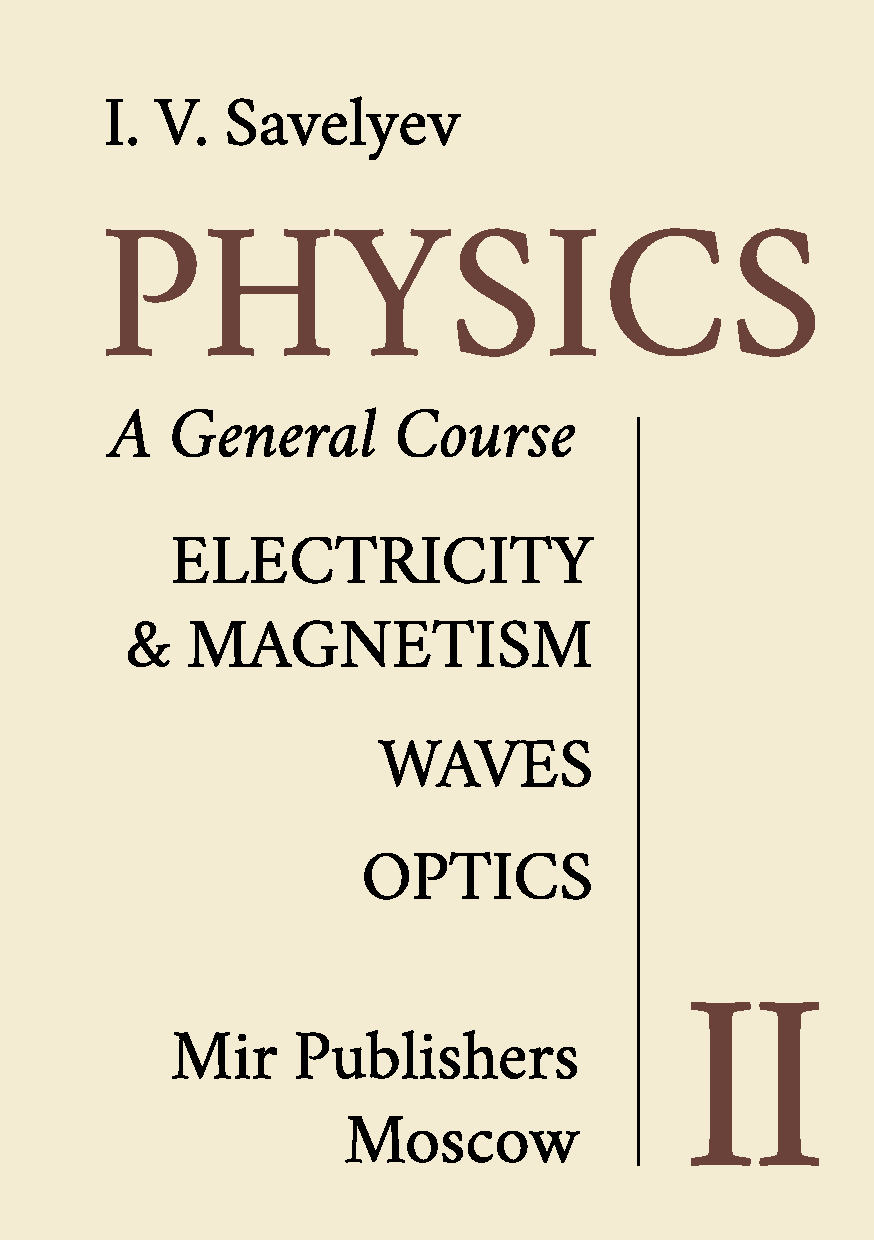
\includepdf{figures/pgc_2_fc.pdf}
\cleardoublepage
% !TEX root = saveliev_physics_general_course_2.tex
%!TEX TS-program = pdflatex
%!TEX encoding = UTF-8 Unicode


%\cleardoublepage
\thispagestyle{empty}
%\maketitle
%\vspace*{1cm}
\noindent
\hspace{50pt}{\large\bfseries I. V. SAVELYEV}
\vspace{40pt}

\noindent
\hspace{50pt}{\Huge\bfseries PHYSICS}
\vspace{10pt}

\noindent
\hspace{50pt}{\Large\bfseries A GENERAL COURSE}
\vspace{10pt}

\noindent
\hspace{50pt}{\bfseries (In three volumes)}
\vspace{30pt}

\noindent
\hspace{120pt}{\Large\bfseries VOLUME~II}
\vspace{12pt}

\noindent
\hspace{120pt}{\huge ELECTRICITY}
\vspace{0.3cm}

\noindent
\hspace{120pt}{\huge AND MAGNETISM}
\vspace{0.5cm}

\noindent
\hspace{120pt}{\huge WAVES}
\vspace{0.5cm}

\noindent
\hspace{120pt}{\huge OPTICS}

\vspace*{3cm}
\hspace{120pt}
\includegraphics[width=0.1\textwidth]{figures/mirlogo.pdf}

\hspace{120pt}{\large MIR PUBLISHERS}

\hspace{120pt}{\large MOSCOW}

%\cleardoublepage
\clearpage

\noindent
Translated from Russian by G. Leib

\vspace{40pt}

%Versi\'on electr\'onica publicada en 2020 por\\[1pt]
%Leandro N. Acquaroli
\noindent
First published 1980

\noindent
Revised from the 1978 Russian edition

\noindent
Second printing 1985

\noindent
Third printing 1989

%\url{http://mirtitles.org}

%The project files are available at:

%\url{https://gitlab.com/mirtitles/pfe}

\vfill
\noindent
\textit{Printed in the Union of Soviet Socialist Republics}

\vspace{30pt}

\noindent
ISBN 5-03-000902-7, 1978

\noindent
ISBN 5-03-000900-0, 1980

\thispagestyle{empty}

\cleardoublepage
% !TEX root = epifanov_solid_state_physics.tex
%!TEX TS-program = pdflatex
%!TEX encoding = UTF-8 Unicode


\chapter*{PREFACE}
\addcontentsline{toc}{chapter}{Preface}
\chaptermark{PREFACE}

\vspace*{-12pt}

Ten years have passed since the first Russian edition of this textbook was published. In this time solid state physics has developed rapidly as the scientific background of numerous front-line branches of technology, absorbing new discoveries and theories. This has been considered in preparing the new edition.

At the same time college curricula have been changed to improve the basic preparation of versatile engineers, especially in physics and mathematics. This too had to be reflected in this book.

Also, the years that have elapsed since the first edition have seen much comment, some critical, and many proposals from Soviet and foreign readers---from college teachers and students, teachers of vocational and secondary schools, engineers and scientists. The author is grateful for all the comment and proposals.

There was a need therefore to revise the book completely. As in the first edition, the presentation of material has followed the aim of elucidating the physical nature of the phenomena discussed. But, where possible, the qualitative relations are also presented, often though without rigorous mathematics.

The manuscript was reviewed in detail by Prof. L. L. Dashkevich, Dr. of Technical Sciences, and Prof. I. G. Nekrashevich, Honored Scientist of the Belorussian Republic. It was perused by Prof. L. A. Gribov, Dr. of Mathematical and Physical Sciences, Assistant Prof. V. B. Zernov, and Z. S. Sazonova. The author extends sincere thanks for their efforts and criticism, which he took into account when revising the manuscript.

The author is also indebted to Senior Lecturer F. Zh. Vilf, Cand. of Technical Sciences, and Assistant Prof. Yu. A. Moma, Cand. of Technical Sciences, for manuals used in this textbook on superconductivity, Gunn effect, and principles of operation of impulse and high-frequency diodes, and to Z. I. Epifanova for all her work in preparing the manuscript.

The author will be most grateful for comment and proposals that might improve this book. They should be sent to the publishers.

\begin{flushright}
	\emph{G. I. E.}
\end{flushright}

%\pagestyle{mystyle}

\cleardoublepage
{\hypersetup{linkcolor=black!80}
	% or \hypersetup{linkcolor=black}, if the colorlinks=true option of hyperref is used
	\tableofcontents
}
\cleardoublepage

\mainmatter

% % !TEX root = saveliev_physics_general_course_1.tex
%!TEX TS-program = pdflatex
%!TEX encoding = UTF-8 Unicode


\chapter*{INTRODUCTION}\label{chap:chapter_introduction}
\addcontentsline{toc}{chapter}{Introduction}
\chaptermark{\sc Introduction}

Physics is a science dealing with the most general properties and forms of motion of matter.

A classical definition of matter was given by V.~Lenin in his book \textit{Materialism and Empirio-Criticism}: ``Matter is a philosophical category denoting the objective reality which is given to man by his sensations, and which is copied, photographed and reflected by our sensations, while existing independently of the''\footnote{V.~I.~Lenin. \textit{Collected Works}, Vol. 14, p. 130. Moscow, Foreign Languages Publishing House (1962).}. Two propositions are significant in this definition, namely, (1) matter is what exists objectively, \ie, independently of anyone's consciousness or sensations, and (2) matter is copied and reflected by our sensations and, consequently, is cognizable.

It follows from the definition of physics that it concentrates knowledge accumulated on the most general properties and phenomena of the world surrounding us. As academician S.~Vavilov noted in one of his articles, ``the extremely common character of a considerable part of the contents of physics, its facts and laws drew physics and philosophy together from time immemorial\ldots. Sometimes physical statements have such a nature that they are difficult to distinguish and separate from philosophical statements, and a physicist must be a philosopher''.

Two kinds of matter are known at present: substance and field. The first kind of matter---substance---includes, for example, atoms, molecules, and all bodies built of them. Electromagnetic, gravitational, and other fields form the second kind of matter. The different kinds of matter can change into each other. For instance, an electron and a positron (representatives of substance) may transform into photons (\ie, into an electromagnetic field). The reverse process is also possible.

Matter is in continuous motion, which is understood to mean any change in general in dialectical materialism\footnote{Dialectical materialism is the name given to the Marxist-Leninist philosophy. The fundamental issue of any philosophy as to what is primary---matter or consciousness---is solved by dialectic materialism in favour of matter when it states that matter is primary and consciousness is secondary. The method of this philosophy is dialectics. It considers matter in constant motion and development whose source is contained in the internal contradictions inherent in objects and phenomena themselves.}. Motion is an inalienable property of matter, which, like matter itself, cannot be created or destroyed. Matter exists and moves in space and in time, which are forms of existence of matter.

The laws of physics are established by generalizing experimental facts. They express the objective regularities existing in nature. These laws are customarily expressed in the form of quantitative relationships between various physical quantities.

The fundamental method of investigation in physics is the running of an experiment, \ie, the observation of the phenomenon being studied in accurately controlled conditions. The latter must permit one to watch the course of the phenomenon and reproduce it each time when these conditions are repeated. Phenomena can be produced experimentally that are not observed in nature. For example, more than ten of the chemical elements known at present have meanwhile not been discovered in nature and were obtained artificially by means of nuclear reactions.

Hypotheses are enlisted to explain experimental data. A hypothesis is a scientific assumption advanced to explain a definite fact or phenomenon and requiring verification and proving to become a scientific theory or law. The correctness of a hypothesis is verified by running the corresponding experiments and by determining whether the corollaries following from the hypothesis agree with the results of experiments and observations. A hypothesis that has successfully passed such verification and has been proved becomes a scientific law or theory.

A physical theory is a system of basic ideas summarizing experimental data and reflecting the objective regularities of nature. A physical theory explains a whole field of natural phenomena from a single viewpoint.

Physics is subdivided into the so-called classical physics and quantum physics. The term classical is applied to the physics whose creation was completed at the beginning of the 20th century. Classical physics was founded by Isaac Newton (1642-1727), who formulated the fundamental laws of classical mechanics. Newtonian mechanics proved to be exceedingly fruitful and mighty, and physicists acquired the conviction that any physical phenomenon can be explained with the aid of Newton's laws.

The edifice of classical physics built up by the end of the last century was very harmonious. Most physicists were convinced that they already knew everything about nature that could be known. The most perspicacious physicists, however, understood that the edifice of classical physics had weak spots. For example, the British physicist William Thomson (Lord Kelvin, 1824-1907) said that there are two dark clouds on the horizon of the cloudless sky of classical physics---the unsuccessful attempts to set up a theory of blackbody radiation, and the contradictory behaviour of ether---the hypothetical medium in which light waves were supposed to propagate. The persistent attempts to surmount these difficulties led to unexpected results. To solve these problems, which were beyond the possibilities of classical physics, it became necessary to revise quite radically the established, habitual notions and introduce concepts that were alien to the spirit of classical physics. Max Planck (1858-1947) succeeded in solving the problem of blackbody radiation in 1900 by introducing the concept of light emission in separate portions---quanta. Thus, at the threshold of the 20th century, the concept of the quantum appeared. It plays an exceedingly important part in modern physics and has resulted in the creation of quantum mechanics. 

The contradictory nature of the experimental facts relating to ether induced Albert Einstein (1879-1955) to revise the notions of space and time that were considered to be obvious from Newton's times. The result was the appearance of the theory of relativity. The latter gives equations of motion appreciably differing from those of Newtonian mechanics for bodies travelling with speeds that are noticeable in comparison with the speed of light.

The year 1897 saw the discovery of the electron. The atoms of all the chemical elements were found to contain these particles. Thus, atoms, previously considered indivisible, appeared to have a complicated structure.

The beginning of the 20th century was thus marked in physics by the radical breaking down of numerous habitual concepts and notions. New physical discoveries and theories destroyed the notions of the structure of matter formed by many physicists. Some of them interpreted this as the vanishing of matter. Many physicists lapsed into idealism, and a crisis began in physics.

V.~Lenin in his book \textit{Materialism and Empirio-Criticism} written in 1908 gave annihilating criticism of ``physical'' idealism. He showed that the new discoveries indicate not the vanishing of matter, but the vanishing of the limit up to which matter was known before that time. ``Matter disappears'', wrote Lenin, ``means that the limit within which we have hitherto known matter disappears and that our knowledge is penetrating deeper; properties of matter are likewise disappearing which formerly seemed absolute, immutable, and primary (impenetrability, inertia, mass, etc.) and which are now revealed to be relative and characteristic only of certain states of matter. For the sole 'property' of matter with whose recognition philosophical materialism is bound up is the property of being an objective reality, of existing outside the mind.''\footnote{V.~I.~Lenin. \textit{Collected Works}, Vol. 14, p. 260. Moscow, Foreign Languages Publishing House (1962).}.

The process of recognizing the world is infinite. Our knowledge at any given stage of development of science is due to the historically achieved level of cognition and cannot be considered as final or complete. It is of necessity relative knowledge, \ie, requires further development, further verification, and more precise definition. At the same time, any truly scientific theory, notwithstanding its relativity and incompleteness, contains elements of absolute, \ie, complete, knowledge, and thus signifies a step in the cognition of the objective world. For instance, mechanics based on Newton's laws is not correct, strictly speaking. But for a certain range of phenomena, this mechanics is quite satisfactory. Thus, the development of science did not cross out Newtonian mechanics. It only established the limits within which it is correct. Newtonian mechanics formed a constituent part of the general edifice of the physical science.

The beginning of the 20th century is characterized by persistent attempts to penetrate into the internal structure of atoms. The key to determining their structure was found to be the studying of atomic spectra. The theory of the atom developed by Niels Bohr (1885-1962) in 1913 was the first striking success in explaining the observed spectra. This theory, however, has obvious features of inconsistency: in addition to the motion of an electron in an atom obeying the laws of classical mechanics, the theory imposes special quantum restrictions on this motion. The theory soon had to pay for this lack of consistency. After the first successes in explaining the spectra of the simplest atom---that of hydrogen---it was found that Bohr's theory is unable to explain the behaviour of atoms with two or more electrons.

The need to develop a new comprehensive theory of atoms became pressing. A bold hypothesis of Louis de Broglie put forward in 1924 placed the cornerstone in such a theory. It was known by that time that light, while being a wave process, also exhibits a corpuscular nature in a number of cases, \ie, behaves like a stream of particles. De Broglie put forth the idea that the particles of a substance, in turn, should display wave properties too in definite conditions. De Broglie's hypothesis soon received a brilliant experimental confirmation---it was proved that a wave process is associated with the particles of a substance, and it must be taken into account when considering the mechanics of an atom. A result of this discovery was the development by Erwin Schr\"odinger (1887-1961) and Werner Heisenberg (1901-1976) of a new physical theory---wave or quantum mechanics. The latter achieved striking successes in explaining atomic processes and the structure of a substance. Results were obtained that showed excellent agreement with experimental data when 'it was found possible to surmount the mathematical difficulties.

The latest decades were noted by remarkable achievements in the field of studying the atomic nucleus. Scientists and engineers have mastered nuclear processes to such an extent that the practical use of nuclear energy has become possible. One of the leading places in this field belongs to Soviet physics. Particularly, the first atomic power plant in the world was erected in the USSR.

Finally, in recent years, the walls of laboratories created by the hands of man were moved apart beyond the limits of our globe. On October 4, 1957, an artificial satellite of the Earth was launched in the Soviet Union the first time in history. It was a small laboratory outfitted with apparatus for scientific research. April 12, 1961, saw the first flight of a man into outer space. The first Soviet cosmonaut, Yuri Gagarin, flew around the Earth and landed safely. The first space rockets were built in the Soviet Union. They left the field of the Earth's attraction and transmitted to the Earth by means of radio signals valuable results of studying outer space and, particularly, photographs of the reverse side of the Moon. In 1969, U.S. astronauts landed on the Moon. In 1975, two Soviet automatic spaceships made a soft landing on Venus and transmitted valuable information on the physical conditions on this planet, and also photographs of its surface.

There is no doubt that the nearest future will be marked with new fundamental discoveries in the science of physics.

%\pagestyle{mystyle}

% \cleardoublepage

\part{ELECTRICITY AND MAGNETISM}\label{part:A}
\cleardoublepage
% !TEX root = saveliev_physics_general_course_2.tex
%!TEX TS-program = pdflatex
%!TEX encoding = UTF-8 Unicode


\chapter{ELECTRIC FIELD IN A VACUUM}\label{chap:1}

\section{Electric Charge}\label{sec:1_1}

All bodies in nature are capable of becoming electrified, \ie, acquiring an electric charge. The presence of such a charge manifests itself in that a charged body interacts with other charged bodies. Two kinds of electric charges exist. They are conventionally called positive and negative. Like charges repel each other, and unlike charges attract each other.

An electric charge is an integral part of certain elementary particles\footnote{Elementary particles are defined as such microparticles whose internal structure at the present level of development of physics cannot be conceived as a combination of other particles.}. The charge of all elementary particles (if it is not absent) is identical in magnitude. It can be called an \textbf{elementary charge}. We shall use the symbol $e$ to denote a positive elementary charge.

The elementary particles include, in particular, the electron (carrying the negative charge $-e$), the proton (carrying the positive charge $+e$), and the neutron (carrying no charge). These particles are the bricks which the atoms and molecules of any substance are built of, therefore all bodies contain electric charges. The particles carrying charges of different signs are usually present in a body in equal numbers and are distributed over it with the same density. The algebraic sum of the charges in any elementary volume of the body equals zero in this case, and each such volume (as well as the body as a whole) will be neutral. If in some way or other we create a surplus of particles of one sign in a body (and, correspondingly, a shortage of particles of the opposite sign), the body will be charged. It is also possible, without changing the total number of positive and negative particles, to cause them to be redistributed in a body so that one part of it has a surplus of charges of one sign and the other part a surplus of charges of the opposite sign. This can be done by bringing a charged body close to an uncharged metal one.

Since a charge $q$ is formed by a plurality of elementary charges, it is an integral multiple of $e$:
\begin{equation}\label{eq:1_1}
	q = \pm N e.
\end{equation}

\noindent
An elementary charge is so small, however, that macroscopic charges may be considered to have continuously changing magnitudes.

If a physical quantity can take on only definite discrete values, it is said to be quantized. The fact expressed by \eqn{1_1} signifies that an electric charge is quantized.

The magnitude of a charge measured in different inertial reference frames will be found to be the same. Hence, an electric charge is relativistically invariant. It thus follows that the magnitude of a charge does not depend on whether the charge is moving or at rest.

Electric charges can vanish and appear again. Two elementary charges of opposite signs always appear or vanish simultaneously, however. For example, an electron and a positron (a positive electron) meeting each other annihilate, \ie, transform into neutral gamma-photons. This is attended by vanishing of the charges $-e$ and $+e$. In the course of the process called the birth of a pair, a gamma-photon getting into the field of an atomic nucleus transforms into a pair of particles---an electron and a positron. This process causes the charges $-e$ and $+e$ to appear.

Thus, the total charge of an electrically isolated system\footnote{A system is referred to as electrically isolated if no charged particles can penetrate through the surface confining it.} cannot change. This statement forms the \textbf{law of electric charge conservation}.

We must note that the law of electric charge conservation is associated very closely with the relativistic invariance of a charge. Indeed, if the magnitude of a charge depended on its velocity, then by bringing charges of one sign into motion we would change the total charge of the relevant isolated system.

\section{Coulomb's Law}\label{sec:1_2}

The law obeyed by the force of interaction of point charges was established experimentally in 1785 by the French physicist Charles A. de Coulomb (1736-1806). A \textbf{point charge} is defined as a charged body whose dimensions may be disregarded in comparison with the distances from this body to other bodies carrying an electric charge.

Using a torsion balance (\fig{1_1}) similar to that employed by H. Cavendish to determine the gravitational constant (see Vol. I, Sec. 6.1), Coulomb measured the force of interaction of two charged spheres depending on the magnitude of the charges on them and on the distance between them. He proceeded from the fact that when a charged metal sphere was touched by an identical uncharged sphere, the charge would be distributed equally between the two spheres.

\begin{figure}[t]
	\begin{center}
		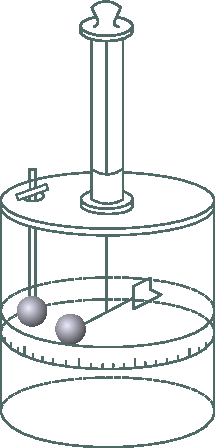
\includegraphics[scale=0.9]{figures/ch_01/fig_1_1.pdf}
		\caption[]{}
		\label{fig:1_1}
	\end{center}
	\vspace{-0.8cm}
\end{figure}

As a result of his experiments, Coulomb arrived at the conclusion that \textit{the force of interaction between two stationary point charges is proportional to the magnitude of each of them and inversely proportional
to the square of the distance between them}. The direction of the force coincides with the straight line connecting the charges.

It must be noted that the direction of the force of interaction along the straight line connecting the point charges follows from considerations of symmetry. An empty space is assumed to be homogeneous and isotropic. Consequently, the only direction distinguished in the space by stationary point charges introduced into it is that from one charge to the other. Assume that the force $\vec{F}$ acting on the charge $q_i$ (\fig{1_2}) makes the angle $\alpha$ with the direction from $q_1$ to $q_2$, and that $\alpha$ differs from $0$ or $\pi$. But owing to axial symmetry, there are no grounds to set the force $\vec{F}$ aside from the multitude of forces of other directions making the same angle $\alpha$ with the axis $q_1$-$q_2$ (the directions of these forces form a cone with a cone angle of $2\alpha$). The difficulty appearing as a result of this vanishes when $\alpha$ equals $0$ or $\pi$.

\begin{figure}[t]
	\begin{minipage}[t]{0.5\linewidth}
		\begin{center}
			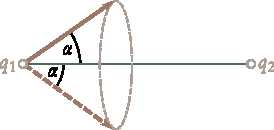
\includegraphics[scale=1]{figures/ch_01/fig_1_2.pdf}
			\caption[]{}
			\label{fig:1_2}
		\end{center}
	\end{minipage}
	\hspace{-0.05cm}
	\begin{minipage}[t]{0.5\linewidth}
		\begin{center}
			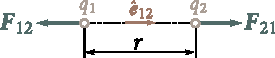
\includegraphics[scale=1]{figures/ch_01/fig_1_3.pdf}
			\caption[]{}
			\label{fig:1_3}
		\end{center}
	\end{minipage}
\vspace{-0.4cm}
\end{figure}

Coulomb's law can be expressed by the formula
\begin{equation}\label{eq:1_2}
	\vec{F}_{12} = -k \frac{q_1 q_2}{r^2}\,\vecuni{12}.
\end{equation}

\noindent
Here, $k$ is a proportionality constant assumed to be positive, $q_1$ and $q_2$ are magnitudes of the interacting charges, $r$ is the distance between the charges, $\vecuni{12}$ is the unit vector directed from the charge $q_1$ to $q_2$ and $\vec{F}_{12}$ is the force acting on the charge $q_1$ (\fig{1_3}; the figure corresponds to the case of like charges).

The force $\vec{F}_{21}$ differs from $\vec{F}_{12}$ in its sign:
\begin{equation}\label{eq:1_3}
	\vec{F}_{21} = k \frac{q_1 q_2}{r^2}\,\vecuni{12}.
\end{equation}

The magnitude of the interaction force, which is the same for both charges, can be written in the form
\begin{equation}\label{eq:1_4}
	F = k \frac{\absolute{q_1 q_2}}{r^2}.
\end{equation}

Experiments show that the force of interaction between two given charges does not change if other charges are placed near them. Assume that we have the charge $\ab{q}{a}$ and, in addition, $N$ other charges $q_1, q_2,\ldots, q_N$. It can be seen from the above that the resultant force $\vec{F}$ with which all the $N$ charges $q_i$ act on $\ab{q}{a}$ is
\begin{equation}\label{eq:1_5}
	\vec{F} = \sum_{i=1}^N \ab{\vec{F}}{a, $i$}
\end{equation}

\noindent
where $\ab{\vec{F}}{a, $i$}$ is the force with which the charge $q_i$ acts on $\ab{q}{a}$ in the absence of the other $N-1$ charges.

The fact expressed by \eqn{1_5} permits us to calculate the force of interaction between charges concentrated on bodies of finite dimensions, knowing the law of interaction between point charges. For this purpose, we must divide each charge into so small charges $\deriv{q}$ that they can be considered as point ones, use \eqn{1_2} to calculate the force of interaction between the charges $\deriv{q}$ taken in pairs, and then perform vector summation of these forces. Mathematically, this procedure coincides completely with the calculation of the force of gravitational attraction between bodies of finite dimensions (see Vol. I, Sec. 6.1).

All experimental facts available lead to the conclusion that Coulomb's law holds for distances from \SI{e-15}{\metre} to at least several kilometres. There are grounds to presume that for distances smaller than \SI{e-16}{\metre} the law stops being correct. For very great distances, there are no experimental confirmations of Coulomb's law. But there are also no reasons to expect that this law stops being obeyed with very great distances between charges.

\section{Systems of Units}\label{sec:1_3}

We can make the proportionality constant in \eqn{1_2} equal unity by properly choosing the unit of charge (the units for $F$ and $r$ were established in mechanics). The relevant unit of charge (when $F$ and $r$ are measured in cgs units) is called the \textbf{absolute electrostatic unit} of charge (cgse$_q$). It is the magnitude of a charge that interacts with a force of \SI{1}{\dyne} in a vacuum with an equal charge at a distance of \SI{1}{\centi\metre} from it.

Careful measurements (they are described in~\sect{10_3}) showed that an elementary charge is
\begin{equation}\label{eq:1_6}
	e = \num{4.80e-10}\text{ cgse$_q$}.
\end{equation}

Adopting the units of length, mass, time, and charge as the basic ones, we can construct a system of units of electrical and magnetic quantities. The system based on the centimetre, gramme, second, and the cgse$_q$ unit is called the \textbf{absolute electrostatic system of units} (the cgse system). It is founded on Coulomb's law, \ie, the law of interaction between charges at rest. On a later page, we shall become acquainted with the \textbf{absolute electromagnetic system of units} (the cgsm system) based on the law of interaction between conductors carrying an electric current. The Gaussian system in which the units of electrical quantities coincide with those of the cgse system, and of magnetic quantities with those of the cgsm system, is also an absolute system.

Equation~\eqref{eq:1_4} in the cgse system becomes
\begin{equation}\label{eq:1_7}
	F = \frac{\absolute{q_1 q_2}}{r^2}.
\end{equation}

\noindent
This equation is correct if the charges are in a vacuum. It has to be determined more accurately for charges in a medium (see \sect{2_8}).

USSR State Standard GOST 9867-61, which came into force on January 1, 1963, prescribes the preferable use of the International System of Units (SI). The basic units of this system are the metre, kilogramme, second, ampere, kelvin, candela, and mole. The SI unit of force is the newton (\si{\newton}) equal to \num{e5} dynes.

In establishing the units of electrical and magnetic quantities, the SI system, like the cgsm one, proceeds from the law of interaction of current-carrying conductors instead of charges. Consequently, the proportionality constant in the equation of Coulomb's law is a quantity with a dimension and differing from unity.

The SI unit of charge is the coulomb (\si{\coulomb}). It has been found experimentally that
% \vspace{-12pt}
\begin{equation}\label{eq:1_8}
	\SI{1}{\coulomb} = \num{2.998e9} \approx \num{3e9}{\text{ cgse$_q$}}.
\end{equation}

To form an idea of the magnitude of a charge of \SI{1}{\coulomb}, let us calculate the force with which two point charges of \SI{1}{\coulomb} each would interact with each other if they were \SI{1}{\metre} apart. By \eqn{1_7}
\begin{equation}\label{eq:1_9}
	F = \frac{\num{3e9}\times\num{3e9}}{100^2}\,\text{ cgse$_F$} = \SI{9e14}{\dyne} = \SI{9e9}{\newton} \approx \SI{e9}{\kgf}.
\end{equation}

An elementary charge expressed in coulombs is
\begin{equation}\label{eq:1_10}
	e = \SI{1.60e-19}{\coulomb}.
\end{equation}

\section{Rationalized Form of Writing Formulas}\label{sec:1_4}

Many formulas of electrodynamics when written in the cgs systems (in particular, in the Gaussian one) include as factors $4\pi$ and the so-called electromagnetic constant $c$ equal to the speed of light in a vacuum. To eliminate these factors in the formulas that are most important in practice, the proportionality constant in Coulomb's law is taken equal to $1/4\pi\varepsilon_0$. The equation of the law for charges in a vacuum will thus become
\begin{equation}\label{eq:1_11}
	F = \frac{1}{4\pi\varepsilon_0}\frac{\absolute{q_1 q_2}}{r^2}.
\end{equation}

\noindent
The other formulas change accordingly. This modified way of writing formulas is called \textbf{rationalized}. Systems of units constructed with the use of rationalized formulas are also called \textbf{rationalized}. They include the SI system.

The quantity $\varepsilon_0$ is called the \textbf{electric constant}. It has the dimension of capacitance divided by length. It is accordingly expressed in units called the farad per metre. To find the numerical value of $\varepsilon_0$, we shall introduce the values of the quantities corresponding to the case of two charges of \SI{1}{\coulomb} each and \SI{1}{\metre} apart into \eqn{1_11}. By \eqn{1_9}, the force of interaction in this case is \SI{9e9}{\newton}. Using this value of the force, and also $q_1=q_2=\SI{1}{\coulomb}$ and $r=\SI{1}{\metre}$ in \eqn{1_11}, we get
\begin{equation*}
	\num{9e9} = \frac{1}{4\pi\varepsilon_0}\frac{\absolute{1\times 1}}{1^2}
\end{equation*}

\noindent
whence
\begin{equation}\label{eq:1_12}
	\varepsilon_0 = \frac{1}{4\pi\times\num{9e9}} = \SI{0.885e-11}{\faraday\per\metre}.
\end{equation}

The Gaussian system of units was widely used and is continuing to be used in physical publications. We therefore consider it essential to acquaint our reader with both the SI and the Gaussian system. We shall set out the material in the SI units showing at the same time how the formulas look in the Gaussian system. The fundamental formulas of electrodynamics written in the SI and the Gaussian system are compared in \app{A_3}.

\section{Electric Field. Field Strength}\label{sec:1_5}

Charges at rest interact through an electric field\footnote{We shall see in \sect{6_2} that when considering moving charges, their interaction in addition to an electric field is due to a magnetic field.}. A charge alters the properties of the space surrounding it---it sets up an electric field in it. This field manifests itself in that an electric charge placed at a point of it experiences the action of a force. Hence, to see whether there is an electric field at a given place, we must place a charged body (in the following we shall say simply a charge for brevity) at it and determine whether or not it experiences the action of an electric force. We can evidently assess the ``strength'' of the field according to the magnitude of the force exerted on the given charge.

Thus, to detect and study an electric field, we must use a ``test'' charge. For the force acting on our test charge to characterize the field ``at the given point'', the test charge must be a point one. Otherwise, the force acting on the charge will characterize the properties of the field averaged over the volume occupied by the body that carries the test charge.

\begin{figure}[t]
	\begin{center}
		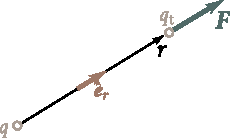
\includegraphics[scale=1]{figures/ch_01/fig_1_4.pdf}
		\caption[]{}
		\label{fig:1_4}
	\end{center}
	\vspace{-0.8cm}
\end{figure}

Let us study the field set up by the stationary point charge $q$ with the aid of the point test charge $\ab{q}{t}$. We place the test charge at a point whose position relative to the charge $q$ is determined by the position vector $\vec{r}$ (\fig{1_4}). We see that the test charge experiences the force
\begin{equation}\label{eq:1_13}
	\vec{F} = \ab{q}{t} \parenthesis{
	\frac{1}{4\pi\varepsilon_0} \frac{q}{r^2}\,\vecuni{r}
	}
\end{equation}

\noindent
[see Eqs. \eqref{eq:1_3} and \eqref{eq:1_11}]. Here $\vecuni{r}$ is the unit vector of the position vector $\vec{r}$.

A glance at \eqn{1_13} shows that the force acting on our test charge depends not only on the quantities determining the field (on $q$ and $\vec{r}$), but also on the magnitude of the test charge $\ab{q}{t}$. If we take different test charges $\ab{q}{t}'$, $\ab{q}{t}''$, etc., then the forces $\vec{F}'$, $\vec{F}''$, etc. which they experience at the given point of the field will be different.
We can see from \eqn{1_13}, however, that the ratio $F/\ab{q}{t}$ for all the test charges will be the same and depend only on the values of $q$ and $\vec{r}$ determining the field at the given point. It is therefore natural to adopt this ratio as the quantity characterizing an electric field:
\begin{equation}\label{eq:1_14}
	\vec{E} = \frac{\vec{F}}{\ab{q}{t}}.
\end{equation}

\noindent
This vector quantity is called the \textbf{electric field strength} (or \textbf{intensity}) at a given point (\ie, at the point where the test charge $\ab{q}{t}$ experiences the action of the force $\vec{F}$).

According to \eqn{1_14}, the electric field strength numerically equals the force acting on a unit point charge at the given point of the field. The direction of the vector $\vec{E}$ coincides with that of the force acting on a positive charge.

It must be noted that \eqn{1_14} also holds when the test charge is negative ($\ab{q}{t}<0$). In this case, the vectors $\vec{E}$ and $\vec{F}$ have opposite directions.

We have arrived at the concept of electric field strength when studying the field of a stationary point charge. Definition \eqref{eq:1_14}, however, also covers the case of a field set up by any collection of stationary charges, but here the following clarification is needed. The arrangement of the charges setting up the field being studied may change under the action of the test charge. This will happen, for example, when the charges producing the field are on a conductor and can freely move within its limits. Therefore, to avoid appreciable alterations in the field being studied, a sufficiently small test charge must be taken.

It follows from Eqs. \eqref{eq:1_13} and \eqref{eq:1_14} that the field strength of a point charge varies directly with the magnitude of the charge $q$ and inversely with the square of the distance $r$ from the charge to the given point of the field:
\begin{equation}\label{eq:1_15}
	\vec{E} = \frac{1}{4\pi\varepsilon_0} \frac{q}{r^2}\, \vecuni{r}.
\end{equation}

\noindent
The vector $\vec{E}$ is directed along the radial straight line passing through the charge and the given point of the field, from the charge if the latter is positive and toward the charge if it is negative.

In the Gaussian system, the equation for the field strength of a point charge in a vacuum has the form
\begin{equation}\label{eq:1_16}
	\vec{E} = \frac{q}{r^2}\, \vecuni{r}.
\end{equation}

The unit of electric field strength is the strength at a point where unit force (\SI{1}{\newton} in the SI and \SI{1}{\dyne} in the Gaussian system) acts on unit charge (\SI{1}{\coulomb} in the SI and \num{1}\cgse{q} in the Gaussian system). This unit has no special name in the Gaussian system. The SI unit of electric field strength is called the volt per metre (\si{\volt\per\metre}) [see \eqn{1_44}].

According to \eqn{1_15}, a charge of \SI{1}{\coulomb} produces the following field strength in a vacuum at a distance of \SI{1}{\metre} from this charge:
\begin{equation*}
	E = \frac{1}{4\pi\parenthesis{1/4\pi \times \num{9e9}}} \frac{1}{1^2} = \SI{9e9}{\volt\per\metre}.
\end{equation*}

This strength in the Gaussian system is
\begin{equation*}
	E = \frac{q}{r^2} = \frac{\num{3e9}}{100^2} = \num{3e5}\cgse{E}.
\end{equation*}

\noindent
Comparing these two results, we find that
\begin{equation}\label{eq:1_17}
	1\cgse{E} = \SI{3e4}{\volt\per\metre}.
\end{equation}

According to \eqn{1_14}, the force exerted on a test charge is
\begin{equation*}
	\vec{F} = \ab{q}{t} \vec{E}.
\end{equation*}

\noindent
It is obvious that any point charge $q$\footnote{In \eqn{1_15}, $q$ stands for the charge setting up the field. In \eqn{1_18}, $q$ stands for the charge experiencing the force $\vec{F}$ at a point of strength $\vec{E}$.} at a point of a field with the strength $\vec{E}$ will experience the force
\begin{equation}\label{eq:1_18}
	\vec{F} = q \vec{E}.
\end{equation}

\noindent
If the charge $q$ is positive, the direction of the force coincides with that of the vector $\vec{E}$. If $q$ is negative, the vectors $\vec{F}$ and $\vec{E}$ are directed oppositely.

We mentioned in \sect{1_2} that the force with which a system of charges acts on a charge not belonging to the system equals the vector sum of the forces which each of the charges of the system exerts separately on the given charge [see \eqn{1_15}]. Hence it follows that \textit{the field strength of a system of charges equals the vector sum of the field strengths that would be produced by each of the charges of the system separately}:
\vspace{-12pt}
\begin{equation}\label{eq:1_19}
	\vec{E} = \sum_i \vec{E}_i.
\end{equation}

\noindent
This statement is called the \textbf{principle of electric field superposition}.

The superposition principle allows us to calculate the field strength of any system of charges. By dividing extended charges into sufficiently
small fractions $\deriv{q}$, we can reduce any system of charges to a collection of point charges. We calculate the contribution of each of such charges to the resultant field by \eqn{1_15}.

An electric field can be described by indicating the magnitude and direction of the vector $\vec{E}$ for each of its points. The combination of these vectors forms the field of the electric field strength vector (compare with the field of the velocity vector, Vol. I, Sec. 9.1). The velocity vector field can be represented very illustratively with the aid of flow lines. Similarly, an electric field can be described with the aid of strength lines, which we shall call for short $\vec{E}$ lines or field lines. These lines are drawn so that a tangent to them at every point coincides with the direction of the vector $\vec{E}$. The density of the lines is selected so that their number passing through a unit area at right angles to the lines equals the numerical value of the vector $\vec{E}$. Hence, the pattern of field lines permits us to assess the direction and magnitude of the vector $\vec{E}$ at various points of space (\fig{1_5}).

\begin{figure}[t]
	\begin{minipage}[t]{0.5\linewidth}
		\begin{center}
			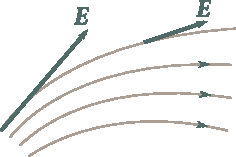
\includegraphics[scale=1]{figures/ch_01/fig_1_5.pdf}
			\caption[]{}
			\label{fig:1_5}
		\end{center}
	\end{minipage}
	\hspace{-0.05cm}
	\begin{minipage}[t]{0.5\linewidth}
		\begin{center}
			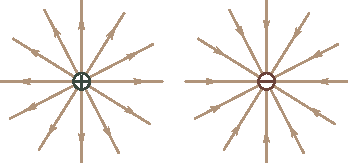
\includegraphics[scale=1]{figures/ch_01/fig_1_6.pdf}
			\caption[]{}
			\label{fig:1_6}
		\end{center}
	\end{minipage}
\vspace{-0.4cm}
\end{figure}

The $\vec{E}$ lines of a point charge field are a collection of radial straight lines directed away from the charge if it is positive and toward it if it is negative (\fig{1_6}). One end of each line is at the charge, and the other extends to infinity. Indeed, the total number of lines intersecting a spherical surface of arbitrary radius $r$ will equal the product of the density of the lines and the surface area of the sphere $4\pi r^2$. We have assumed that the density of the lines numerically equals $E=(1/4\pi\varepsilon_0)(q/r^2)$. Hence, the number of lines is $(1/4\pi\varepsilon_0)(q/r^2) 4\pi r^2=q/\varepsilon_0$. This result signifies that the number of lines at any distance from a charge will be the same. It thus follows hat the lines do not begin and do not terminate anywhere except tor the charge. Beginning at the charge, they extend to infinity (the charge is positive), or arriving from infinity, they terminate at the charge (the latter is negative). This property of the $\vec{E}$ lines is common for all electrostatic fields, \ie, fields set up by any system of stationary charges: the field lines can begin or terminate only at charges or extend to infinity.

\section{Potential}\label{sec:1_6}

Let us consider the field produced by a stationary point charge $q$. At any point of this field, the point charge $q'$ experiences the force
\begin{equation}\label{eq:1_20}
	\vec{F} = \frac{1}{4\pi\varepsilon_0}\frac{qq'}{r^2}\, \vecuni{r} = F(r)\vecuni{r}.
\end{equation}

\noindent
Here $F(r)$ is the magnitude of the force $\vec{F}$, and $\vecuni{r}$ is the unit vector of the position vector $\vec{r}$ determining the position of the charge $q'$ relative to the charge $q$.

\begin{figure}[t]
	\begin{center}
		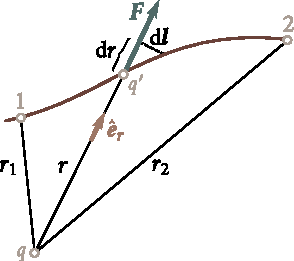
\includegraphics[scale=1]{figures/ch_01/fig_1_7.pdf}
		\caption[]{}
		\label{fig:1_7}
	\end{center}
	\vspace{-0.8cm}
\end{figure}

The force \eqref{eq:1_20} is a central one (see Vol. I, Sec. 3.4). A central field of forces is conservative. Consequently, the work done by the forces of the field on the charge $q'$ when it is moved from one point to another does not depend on the path. This work is
\begin{equation}\label{eq:1_21}
	A_{12} = \int_1^2 F(r) \vecuni{r}\, \deriv{\vec{l}}
\end{equation}

\noindent
where $\deriv{\vec{l}}$ is the elementary displacement of the charge $q'$. Inspection of \fig{1_7} shows that the scalar product $\vecuni{r}\,\deriv{\vec{l}}$ equals the increment of the magnitude of the position vector $\vec{r}$, \ie, $\deriv{r}$. Equation \eqref{eq:1_21} can therefore be written in the form
\begin{equation*}
	A_{12} = \int_1^2 F(r)\, \deriv{r}
\end{equation*}

\noindent
[compare with Eq. (3.24) of Vol. I]. Introduction of the expression for $F(r)$ yields
\begin{equation}\label{eq:1_22}
	A_{12} = \frac{qq'}{4\pi\varepsilon_0} \int_{r_1}^{r_2} \frac{\deriv{r}}{r^2} = \frac{1}{4\pi\varepsilon_0} \parenthesis{
	\frac{qq'}{r_1} - \frac{qq'}{r_2}
	}.
\end{equation}

The work of the forces of a conservative field can be represented as a decrement of the potential energy:
\begin{equation}\label{eq:1_23}
	A_{12} = \ab{W}{p,$1$} - \ab{W}{p,$2$}.
\end{equation}

\noindent
A comparison of Eqs. \eqref{eq:1_22} and \eqref{eq:1_23} leads to the following expression for the potential energy of the charge $q'$ in the field of the charge $q$:
\begin{equation*}
	\ab{W}{p} = \frac{1}{4\pi\varepsilon_0} \frac{qq'}{r_2} + \text{constant}.
\end{equation*}

\noindent
The value of the constant in the expression for the potential energy is usually chosen so that when the charge moves away to infinity (\ie, when $r=\infty$), the potential energy vanishes. When this condition is observed, we get
\begin{equation}\label{eq:1_24}
	\ab{W}{p} = \frac{1}{4\pi\varepsilon_0} \frac{qq'}{r_2}.
\end{equation}

Let us use the charge $q'$ as a test charge for studying the field. By \eqn{1_24}, the potential energy which the test charge has depends not only on its magnitude $q'$, but also on the quantities $q$ and $r$ determining the field. Thus, we can use this energy to describe the field just like we used the force acting on the test charge for this purpose.

Different test charges $\ab{q}{t}'$, $\ab{q}{t}''$, etc. will have different energies $\ab{W}{p}'$, $\ab{W}{p}''$, etc. at the same point of a field. But the ratio $\ab{W}{p}/\ab{q}{t}$ will be the same for all the charges [see \eqn{1_24}]. The quantity
\begin{equation}\label{eq:1_25}
	\varphi = \frac{\ab{W}{p}}{\ab{q}{t}}
\end{equation}

\noindent
is called the \textbf{field potential} at a given point and is used together with the field strength $\vec{E}$ to describe electric fields.

It can be seen from \eqn{1_25} that the potential numerically equals the potential energy which a unit positive charge would have at the given point of the field. Substituting for the potential energy in \eqn{1_25} its value from \eqref{eq:1_24}, we get the following expression for the potential of a point charge:
\begin{equation}\label{eq:1_26}
	\varphi = \frac{1}{4\pi\varepsilon_0} \frac{q}{r}.
\end{equation}

In the Gaussian system, the potential of the field of a point charge in a vacuum is determined by the formula
\begin{equation}\label{eq:1_27}
	\varphi = \frac{q}{r}.
\end{equation}

Let us consider the field produced by a system of $N$ point charges $q_1, q_2,\ldots, q_N$. Let $r_1, r_2,\ldots, r_N$ be the distances from each of the charges to the given point of the field. The work done by the forces of this field on the charge $q'$ will equal the algebraic sum of the work done by the forces set up by each of the charges separately:
\begin{equation*}
	A_{12} = \sum_{i=1}^N A_i.
\end{equation*}

\noindent
By \eqn{1_22}, each work $A_i$ equals
\begin{equation*}
	A_{i} = \frac{1}{4\pi\varepsilon_0} \parenthesis{
	\frac{q_i q'}{r_{i,1}} - \frac{q_i q'}{r_{i,2}}
	}
\end{equation*}

\noindent
where $r_{i,1}$ is the distance from the charge $q_i$ to the initial position of the charge $q'$, and $r_{i,2}$ is the distance from $q_i$ to the final position of the charge $q'$. Hence,
\begin{equation*}
	A_{i2} = \frac{1}{4\pi\varepsilon_0} \sum_{i=1}^N \frac{q_i q'}{r_{i,1}} - \frac{1}{4\pi\varepsilon_0} \sum_{i=1}^N \frac{q_i q'}{r_{i,2}}.
\end{equation*}

\noindent
Comparing this equation with \eqn{1_23}, we get the following expression for the potential energy of the charge $q'$ in the field of a system of charges:
\begin{equation*}
	\ab{W}{p} = \frac{1}{4\pi\varepsilon_0} \sum_{i=1}^N \frac{q_i q'}{r_{i}}
\end{equation*}

\noindent
from which it can be seen that
\begin{equation}\label{eq:1_28}
	\varphi = \frac{1}{4\pi\varepsilon_0} \sum_{i=1}^N \frac{q_i}{r_{i}}.
\end{equation}

Comparing this formula with \eqn{1_26}, we arrive at the conclusion that \textit{the potential of the field produced by a system of charge equals the algebraic sum of the potentials produced by each of the charges separately}. Whereas the field strengths are added vectorially in the superposition of fields, the potentials are added algebraically. This is why it is usually much simpler to calculate the potentials than the electric field strengths.

Examination of \eqn{1_25} shows that the charge $q$ at a point of a field with the potential $\varphi$ has the potential energy
\begin{equation}\label{eq:1_29}
	\ab{W}{p} = q\varphi.
\end{equation}

\noindent
Hence, the work of the field forces on the charge $q$ can be expressed through the potential difference:
\begin{equation}\label{eq:1_30}
	A_{12} = \ab{W}{p,$1$} - \ab{W}{p,$2$} = q \parenthesis{\varphi_1 - \varphi_2}.
\end{equation}

\noindent
Thus, the work done on a charge by the forces of a field equals the product of the magnitude of the charge and the difference between the potentials at the initial and final points (\ie, the potential decrement).

If the charge $q$ is removed from a point having the potential $\varphi$ to infinity (where by convention the potential vanishes), then the work of the field forces will be
\begin{equation}\label{eq:1_31}
	A_{\infty} = q \varphi.
\end{equation}

\noindent
Here, it follows that the potential numerically equals the work done by the forces of a field on a unit positive charge when the latter is removed from the given point to infinity. Work of the same magnitude must be done against the electric field forces to move a unit positive charge from infinity to the given point of a field.

Equation \eqref{eq:1_31} can be used to establish the units of potential. The unit of potential is taken equal to the potential at a point of a field when work equal to unity is required to move unit positive charge from infinity to this point. The SI unit of potential called the volt (\si{\volt}) is taken equal to the potential at a point when work of $1$ joule has to be done to move a charge of $1$ coulomb from infinity to this point:
\begin{equation}\label{eq:1_32}
	\SI{1}{\joule} = \SI{1}{\coulomb} \times \SI{1}{\volt},\quad  \text{thus,}\quad \SI{1}{\volt} = \frac{\SI{1}{\joule}}{\SI{1}{\coulomb}}.
\end{equation}

The absolute electrostatic unit of potential (\cgse{\varphi}) is taken equal to the potential at a point when work of \SI{1}{\erg} has to be done to move a charge of \num{+1}\cgse{q} from infinity to this point. Expressing \SI{1}{\joule} and \SI{1}{\coulomb} in \eqn{1_32} through cgse units, we shall find the relation between the volt and the cgse potential unit:
\begin{equation}\label{eq:1_33}
	\SI{1}{\volt} = \frac{\SI{1}{\joule}}{\SI{1}{\coulomb}} = \frac{\SI{e7}{\erg}}{\num{3e9}\cgse{q}} = \frac{1}{300}\cgse{\varphi}.
\end{equation}

\noindent
Thus, $1$\cgse{\varphi} equals \SI{300}{\volt}.

A unit of energy and work called the \textbf{electron-volt} (\si{\electronvolt}) is frequently used in physics. An electron-volt is defined as the work done by the forces of a field on a charge equal to that of an electron (\ie, on the elementary charge $e$) when it passes through a potential difference of \SI{1}{\volt}:
\begin{equation}\label{eq:1_34}
	\SI{1}{\electronvolt} = \SI{1.60e-19}{\coulomb} \times \SI{1}{\volt} = \SI{1.60e-19}{\joule} = \SI{1.60e-12}{\erg}.
\end{equation}

\noindent
Multiple units of the electron-volt are also used:
\begin{align*}
	\text{\SI{1}{\kilo\electronvolt} (kiloelectron-volt)} &= \SI{e3}{\electronvolt},\\
	\text{\SI{1}{\mega\electronvolt} (megaelectron-volt)} &= \SI{e6}{\electronvolt},\\
	\text{\SI{1}{\giga\electronvolt} (gigaelectron-volt)} &= \SI{e9}{\electronvolt}.
\end{align*}

\section{Interaction Energy of a System of Charges}\label{sec:1_7}

Equation \eqref{eq:1_24} can be considered as the mutual potential energy of the charges $q$ and $q'$. Using the symbols $q_1$ and $q_2$ for these charges, we get the following formula for their interaction energy:
\begin{equation}\label{eq:1_35}
	\ab{W}{p} = \frac{1}{4\pi\varepsilon_0} \frac{q_1q_2}{r_{12}}.
\end{equation}

\noindent
The symbol $r_{12}$ stands for the distance between the charges.

Let us consider a system consisting of $N$ point charges $q_1, q_2, \ldots, q_N$. We showed in Sec. 3.6 of Vol. I that the energy of interaction of such a system equals the sum of the energies of interaction of the charges taken in pairs:
\begin{equation}\label{eq:1_36}
	\ab{W}{p} = \frac{1}{2} \sum_{(i\neq k)} \ab{W}{p,$ik$}(r_{ik})
\end{equation}

\noindent
[see Eq. (3.60) of Vol. I].

According to \eqn{1_35}
\begin{equation*}
	\ab{W}{p,$ik$} = \frac{1}{4\pi\varepsilon_0} \frac{q_i q_k}{r_{ik}}.
\end{equation*}

\noindent
Using this equation in \eqref{eq:1_36}, we find that
\begin{equation}\label{eq:1_37}
	\ab{W}{p} = \frac{1}{2} \sum_{(i\neq k)} \frac{1}{4\pi\varepsilon_0} \frac{q_i q_k}{r_{ik}}.
\end{equation}

In the Gaussian system, the factor $1/(4\pi\varepsilon_0)$ is absent in this equation.

In \eqn{1_37}, summation is performed over the subscripts $i$ and $k$. Both subscripts pass independently through all the values from $1$ to $N$. Addends for which the value of the subscript $i$ coincides with that of $k$ are not taken into consideration. Let us write \eqn{1_37}
as follows:
\begin{equation}\label{eq:1_38}
	\ab{W}{p} = \frac{1}{2} \sum_{i=1}^N q_i \sum_{\substack{{i=1}\\ (i\neq k)}}^N \frac{1}{4\pi\varepsilon_0} \frac{q_k}{r_{ik}}.
\end{equation}

\noindent
The expression
\begin{equation*}
	\varphi_i =  \frac{1}{4\pi\varepsilon_0} \sum_{\substack{{i=1}\\ (i\neq k)}}^N \frac{q_k}{r_{ik}}
\end{equation*}

\noindent
is the potential produced by all the charges except $q_i$ at the point where the charge $q_i$ is. With this in view, we get the following formula for the interaction energy:
\begin{equation}\label{eq:1_39}
	\ab{W}{p} = \frac{1}{2} \sum_{i=1}^N q_i \varphi_i.
\end{equation}

\section{Relation Between Electric Field Strength and Potential}\label{sec:1_8}

An electric field can be described either with the aid of the vector quantity $\vec{E}$, or with the aid of the scalar quantity $\varphi$. There must evidently be a definite relation between these quantities. If we bear in mind that $\vec{E}$ is proportional to the force acting on a charge and $\varphi$ to the potential energy of the charge, it is easy to see that this relation must be similar to that between the potential energy and the force.

The force $\vec{F}$ is related to the potential energy by the expression
\begin{equation}\label{eq:1_40}
	\vec{F} = -\nabla\ab{W}{p}
\end{equation}

\noindent
[see Eq. (3.32) of Vol. I]. For a charged particle in an electrostatic field, we have $\vec{F}=q\vec{E}$ and $\ab{W}{p}=q\varphi$. Introducing these values into \eqn{1_40}, we find that
\begin{equation*}
	q \vec{E} = -\nabla(q\varphi).
\end{equation*}

\noindent
The constant $q$ can be put outside the gradient sign. Doing this and then cancelling $q$, we arrive at the formula
\begin{equation}\label{eq:1_41}
	\vec{E} = -\nabla\varphi
\end{equation}

\noindent
establishing the relation between the field strength and potential.

Taking into account the definition of the gradient [see Eq. (3.31) of Vol. 1], we can write that
\begin{equation}\label{eq:1_42}
	\vec{E} = -\diffpartial{\varphi}{x}\vecuni{x} -\diffpartial{\varphi}{y}\vecuni{y} -\diffpartial{\varphi}{z}\vecuni{z}.
\end{equation}

\noindent
Hence, \eqn{1_41} has the following form in projections onto the coordinate axes:
\begin{equation}\label{eq:1_43}
	E_x = -\diffpartial{\varphi}{x},\quad E_y = -\diffpartial{\varphi}{y},\quad E_z = -\diffpartial{\varphi}{z}.
\end{equation}

\noindent
Similarly, the projection of the vector $\vec{E}$ onto an arbitrary direction $l$ equals the derivative of $\varphi$ with respect to $l$ taken with the opposite sign, \ie, the rate of diminishing of the potential when moving along the direction $l$:
\begin{equation}\label{eq:1_44}
	E_l = -\diffpartial{\varphi}{l}.
\end{equation}

\noindent
It is easy to see that \eqn{1_44} is correct by choosing $l$ as one of the coordinate axes and taking \eqn{1_43} into account.

Let us explain \eqn{1_41} using as an example the field of a point charge. The potential of this field is expressed by \eqn{1_26}. Passing over to Cartesian coordinates, we get the expression
\begin{equation*}
	\varphi = \frac{1}{4\pi\varepsilon_0} \frac{q}{r} = \frac{1}{4\pi\varepsilon_0} \frac{q}{\parenthesis{x^2 + y^2 + z^2}^{1/2}}.
\end{equation*}

\noindent
The partial derivative of this function with respect to $x$ is
\begin{equation*}
	\diffpartial{\varphi}{x} = -\frac{1}{4\pi\varepsilon_0} \frac{qx}{\parenthesis{x^2 + y^2 + z^2}^{3/2}} = -\frac{1}{4\pi\varepsilon_0} \frac{qx}{r^3}.
\end{equation*}

\noindent
Similarly,
\begin{equation*}
	\diffpartial{\varphi}{y} = -\frac{1}{4\pi\varepsilon_0} \frac{qy}{r^3},\quad \diffpartial{\varphi}{y} = -\frac{1}{4\pi\varepsilon_0} \frac{qz}{r^3}.
\end{equation*}

\noindent
Using the found values of the derivatives in \eqn{1_42}, we arrive
at the expression
\begin{equation*}
	\vec{E} = \frac{1}{4\pi\varepsilon_0} \frac{q \parenthesis{x\vecuni{x}+y\vecuni{y}+z\vecuni{z}}}{r^3} = \frac{1}{4\pi\varepsilon_0} \frac{q\vec{r}}{r^3} = \frac{1}{4\pi\varepsilon_0} \frac{q}{r^2}\,\vecuni{r}
\end{equation*}

\noindent
that coincides with \eqn{1_15}.

Equation \eqref{eq:1_41} allows us to find the field strength at every point from the known values of $\varphi$. We can also solve the reverse problem, \ie, find the potential difference between two arbitrary points of a field according to the given values of $\vec{E}$. For this purpose, we shall take advantage of the circumstance that the work done by the forces of a field on the charge $q$ when it is moved from point $1$ to point $2$ can be calculated as
\begin{equation*}
	A_{12} = \int_1^2 q \vec{E}\, \deriv{\vec{l}}.
\end{equation*}

\noindent
At the same time in accordance with \eqn{1_30}, this work can be written as
\begin{equation*}
	A_{12} = q \parenthesis{\varphi_1 - \varphi_2}.
\end{equation*}

\noindent
Equating these two expressions and cancelling $q$, we obtain
\begin{equation}\label{eq:1_45}
	\varphi_1 - \varphi_2 = \int_1^2 \vec{E}\, \deriv{\vec{l}}.
\end{equation}

\noindent
The integral can be taken along any line joining points $1$ and $2$ because the work of the field forces is independent of the path. For circumvention along a closed contour, $\varphi_1=\varphi_2$, and \eqn{1_45} becomes
\begin{equation}\label{eq:1_46}
	\oint \vec{E}\, \deriv{\vec{l}} = 0
\end{equation}

\noindent
(the circle on the integral sign indicates that integration is performed over a closed contour). It must be noted that this relation holds only for an electrostatic field. We shall see on a later page that the field of moving charges (\ie, a field changing with time) is not a potential one. Therefore, condition \eqref{eq:1_46} is not observed for it.

An imaginary surface all of whose points have the same potential is called an equipotential surface. Its equation has the form
\begin{equation*}
	\varphi(x,y,z) = \text{constant}.
\end{equation*}

\noindent
The potential does not change in movement along an equipotential surface over the distance $\deriv{l}$ ($\deriv{\varphi}=0$). Hence, according to \eqn{1_44}, the tangential component of the vector $\vec{E}$ to the surface equals zero. We thus conclude that the vector $\vec{E}$ at every point is directed along a normal to the equipotential surface passing through the given point. Bearing in mind that the vector $\vec{E}$ is directed along a tangent to an $\vec{E}$ line, we can easily see that the field lines at every point are orthogonal to the equipotential surfaces.

An equipotential surface can be drawn through any point of a field. Consequently, we can construct an infinitely great number of such surfaces. They are conventionally drawn so that the potential difference for two adjacent surfaces is the same everywhere. Thus, the density of the equipotential surfaces allows us to assess the magnitude of the field strength. Indeed, the denser are the equipotential surfaces, the more rapidly does the potential change when moving along a normal to the surface. Hence, $\nabla\varphi$ is greater at the given place, and, therefore, $\vec{E}$ is greater too.

Figure \ref{fig:1_8} shows equipotential surfaces (more exactly, their intersections with the plane of the drawing) for the field of a point charge. In accordance with the nature of the dependence of $E$ on $r$, equipotential surfaces become the denser, the nearer we approach
a charge.

\begin{figure}[t]
	\begin{minipage}[t]{0.5\linewidth}
		\begin{center}
			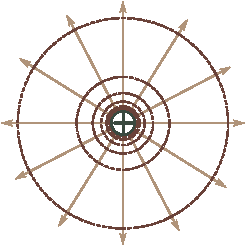
\includegraphics[scale=1]{figures/ch_01/fig_1_8.pdf}
			\caption[]{}
			\label{fig:1_8}
		\end{center}
	\end{minipage}
	\hspace{-0.05cm}
	\begin{minipage}[t]{0.5\linewidth}
		\begin{center}
			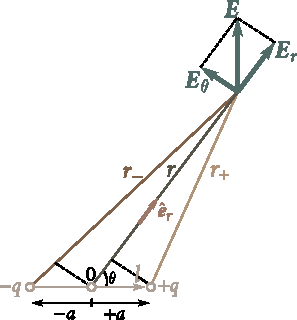
\includegraphics[scale=0.95]{figures/ch_01/fig_1_9.pdf}
			\caption[]{}
			\label{fig:1_9}
		\end{center}
	\end{minipage}
\vspace{-0.4cm}
\end{figure}

Equipotential surfaces for a homogeneous field are a collection of equispaced planes at right angles to the direction of the field.

\section{Dipole}\label{sec:1_9}

An \textbf{electric dipole} is defined as a system of two point charges $+q$ and $-q$ identical in value and opposite in sign, the distance between which is much smaller than that to the points at which the field of the system is being determined. The straight line passing through both charges is called the \textbf{dipole axis}.

Let us first calculate the potential and then the field strength of a dipole. This field has axial symmetry. Therefore, the pattern of the field in any plane passing through the dipole axis will be the same, the vector $\vec{E}$ being in this plane. The position of a point relative to the dipole will be characterized with the aid of the position vector $\vec{r}$ or with the aid of the polar coordinates $r$ and $\theta$ (\fig{1_9}). We shall introduce the vector $\vec{l}$ passing from the negative charge to the positive one. The position of the charge $+q$ relative to the centre of the dipole is determined by the vector $\vec{a}$, and of the charge $-q$ by the vector $-\vec{a}$. It is obvious that $\vec{l}=2\vec{a}$. We shall designate the distances to a given point from the charges $+q$ and $-q$ by $r_+$ and $r_-$, respectively.

Owing to the smallness of $a$ in comparison with $r$, we can assume approximately that
\begin{equation}\label{eq:1_47}
\begin{split}
	r_+ &= r - a\cos\theta = r - \vec{a}\!\vec{\cdot}\!\vecuni{r},\\
	r_- &= r + a\cos\theta = r + \vec{a}\!\vec{\cdot}\!\vecuni{r}.
\end{split}
\end{equation}

The potential at a point determined by the position vector $\vec{r}$ is
\begin{equation*}
	\varphi(\vec{r}) = \frac{1}{4\pi\varepsilon_0} \parenthesis{
	\frac{q}{r_+} - \frac{q}{r_-}
	} = \frac{1}{4\pi\varepsilon_0} \frac{q(r_- - r_+)}{r_+ r_-}.
\end{equation*}

\noindent
The product $r_+r_-$ can be replaced with $r^2$. The difference $r_--r_+$ according to Eqs. \eqref{eq:1_47}, is $2(\vec{a}\!\vec{\cdot}\!\vecuni{r})=\vec{l}\!\vec{\cdot}\!\vecuni{r}$. Hence,
\begin{equation}\label{eq:1_48}
	\varphi(\vec{r}) = \frac{1}{4\pi\varepsilon_0} \frac{q(\vec{l}\!\vec{\cdot}\!\vecuni{r})}{r^2} = \frac{1}{4\pi\varepsilon_0} \frac{(\vec{p}\!\vec{\cdot}\!\vecuni{r})}{r^2}
\end{equation}

\noindent
where
\begin{equation}\label{eq:1_49}
	\vec{p} = q\vec{l}
\end{equation}

\noindent
is a characteristic of a dipole called its \textbf{electric moment}. The vector $\vec{p}$ is directed along the dipole axis from the negative charge to the positive one (\fig{1_10}).

\begin{figure}[t]
	\begin{center}
		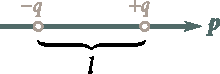
\includegraphics[scale=1.1]{figures/ch_01/fig_1_10.pdf}
		\caption[]{}
		\label{fig:1_10}
	\end{center}
	\vspace{-0.8cm}
\end{figure}

A glance at \eqn{1_48} shows that the field of a dipole is determined by its electric moment $\vec{p}$. We shall see below that the behaviour of a dipole in an external electric field is also determined by its electric moment $\vec{p}$. A comparison with \eqn{1_26} shows that the potential of a dipole field diminishes with the distance more rapidly (as $1/r^2$) than the potential of a point charge field (which changes in proportion to $1/r$).

It can be seen from \fig{1_9} that $\vec{p}\!\vec{\cdot}\!\vecuni{r}=p\cos\theta$. Therefore, \eqn{1_48} can be written as follows:
\begin{equation}\label{eq:1_50}
	\varphi(r,\theta) = \frac{1}{4\pi\varepsilon_0} \frac{p\cos\theta}{r^2}.
\end{equation}

To find the field strength of a dipole, let us calculate the projections of the vector $\vec{E}$ onto two mutually perpendicular directions by \eqn{1_44}. One of them is determined by the motion of a point due to the change in the distance $r$ (with $\theta$ fixed), the other by the motion of the point due to the change in the angle $\theta$ (with $r$ fixed, see \fig{1_9}). The first projection is obtained by differentiation of \eqn{1_50} with respect to $r$:
\begin{equation}\label{eq:1_51}
	E_r = - \diffpartial{\varphi}{r} = \frac{1}{4\pi\varepsilon_0} \frac{2p\cos\theta}{r^3}.
\end{equation}

\noindent
We shall find the second projection (let us designate it by $E_{\theta}$) by taking the ratio of the increment of the potential $\varphi$ obtained when the angle $\theta$ grows by $\deriv{\theta}$ to the distance $r\,\deriv{\theta}$ over which the end of the segment $r$ moves (in this case the quantity $\deriv{l}$ in \eqn{1_44} equals $r\,\deriv{\theta}$]. Thus,
\begin{equation*}
	E_{\theta} = - \frac{1}{r}\diffpartial{\varphi}{\theta}.
\end{equation*}

\noindent
Introducing the value of the derivative of function \eqref{eq:1_50} with respect to $\theta$ we get
\begin{equation}\label{eq:1_52}
	E_{\theta} = \frac{1}{4\pi\varepsilon_0} \frac{p\sin\theta}{r^3}.
\end{equation}

\noindent
The sum of the squares of Eqs. \eqref{eq:1_51} and \eqref{eq:1_52} gives the square of the vector $\vec{E}$ (see \fig{1_9}):
\begin{align*}
	E^2 &= E_r^2 + E_{\theta}^2 = \parenthesis{\frac{1}{4\pi\varepsilon_0}}^2 \parenthesis{\frac{p}{r^3}}^2 \parenthesis{4\cos^2\theta + \sin^2\theta}\\
		&= \parenthesis{\frac{1}{4\pi\varepsilon_0}}^2 \parenthesis{\frac{p}{r^3}}^2 \parenthesis{1 + 3\cos^2\theta}.
\end{align*}

\noindent
Hence
\begin{equation}\label{eq:1_53}
	E = \frac{1}{4\pi\varepsilon_0} \frac{p}{r^3} \parenthesis{1 + 3\cos^2\theta}^{1/2}.
\end{equation}

Assuming in \eqn{1_53} that $\theta=0$, we get the strength on the dipole axis:
\begin{equation}\label{eq:1_54}
	E_{\parallel} = \frac{1}{4\pi\varepsilon_0} \frac{2p}{r^3}.
\end{equation}

\noindent
The vector $\vec{E}_{\parallel}$ is directed along the dipole axis. This is in agreement with the axial symmetry of the problem. Examination of \eqn{1_51} shows that $E_r>0$ when $\theta=0$, and $E_r<0$ when $\theta=\pi$. This signifies that in any case the vector $\vec{E}_{\parallel}$ has a direction coinciding with that from $-q$ to $+q$ (\ie, with the direction of $\vec{p}$). Equation \eqref{eq:1_54} can therefore be written in the vector form:
\begin{equation}\label{eq:1_55}
	\vec{E}_{\parallel} = \frac{1}{4\pi\varepsilon_0} \frac{2\vec{p}}{r^3}.
\end{equation}

Assuming in \eqn{1_53} that $\theta=\pi/2$, we get the field strength on the straight line passing through the centre of the dipole and perpendicular to its axis:
\begin{equation}\label{eq:1_56}
	E_{\perp} = \frac{1}{4\pi\varepsilon_0} \frac{p}{r^3}.
\end{equation}

\noindent
By \eqn{1_51}, when $\theta=\pi/2$, the projection $E_r$ equals zero. Hence, the vector $\vec{E}_{\perp}$ is parallel to the dipole axis. It follows from \eqn{1_52} that when $\theta=\pi/2$, the projection $E_{\theta}$ is positive. This signifies that the vector $\vec{E}_{\perp}$ is directed toward the growth of the angle $\theta$, \ie, antiparallel to the vector $\vec{p}$.

The field strength of a dipole is characterized by the circumstance that it diminishes with the distance from the dipole in proportion to $1/r^3$, \ie, more rapidly than the field strength of a point charge (which diminishes in proportion to $1/r^2$).

\begin{figure}[t]
	\begin{minipage}[t]{0.5\linewidth}
		\begin{center}
			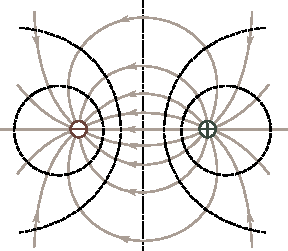
\includegraphics[scale=1]{figures/ch_01/fig_1_11.pdf}
			\caption[]{}
			\label{fig:1_11}
		\end{center}
	\end{minipage}
	\hspace{-0.05cm}
	\begin{minipage}[t]{0.5\linewidth}
		\begin{center}
			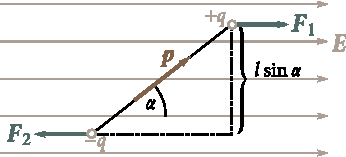
\includegraphics[scale=1]{figures/ch_01/fig_1_12.pdf}
			\caption[]{}
			\label{fig:1_12}
		\end{center}
	\end{minipage}
\vspace{-0.4cm}
\end{figure}

Figure \ref{fig:1_11} shows $\vec{E}$ lines (the solid lines) and equipotential surfaces (the dash lines) of the field of a dipole. According to \eqn{1_50}, when $\theta=\pi/2$, the potential vanishes for all the $r$'s. Thus, all the points of a plane at right angles to the dipole axis and passing through its middle have a zero potential. This could have been predicted because the distances from the charges $+q$ and $-q$ to any point of this plane are identical.

Now let us turn to the behaviour of a dipole in an external electric field. If a dipole is placed in a homogeneous electric field, the charges $+q$ and $-q$ forming the dipole will be under the action of the forces $\vec{F}_1$ and $\vec{F}_2$ equal in magnitude, but opposite in direction (\fig{1_12}). These forces form a couple whose arm is $l\sin\alpha$, \ie, depends on the orientation of the dipole relative to the field. The magnitude of each of the forces is $qE$. Multiplying it by the arm, we get the magnitude of the torque acting on a dipole:
\begin{equation}\label{eq:1_57}
	T = q E l \sin\alpha = p E \sin\alpha
\end{equation}

\noindent
($p$ is the electric moment of the dipole). It is easy to see that \eqn{1_57} can be written in the vector form
\begin{equation}\label{eq:1_58}
	\vec{T} = \vecprod{p}{E}.
\end{equation}

\noindent
The torque \eqref{eq:1_58} tends to turn a dipole so that its electric moment $\vec{p}$ is in the direction of the field.

Let us find the potential energy belonging to a dipole in an external electric field. By \eqn{1_29}, this energy is
\begin{equation}\label{eq:1_59}
	\ab{W}{p} = q\varphi_+ - q\varphi_- = q(\varphi_+ - \varphi_-).
\end{equation}

\noindent
Here $\varphi_+$ and $\varphi_-$ are the values of the potential of the external field at the points where the charges $+q$ and $-q$ are placed.

The potential of a homogeneous field diminishes linearly in the direction of the vector $\vec{E}$. Assuming that the $x$-axis is this direction (\fig{1_13}), we can write that $E=E_x=-\diffin{\varphi}{x}$. A glance at \fig{1_13} shows that the difference $\varphi_+-\varphi_-$ equals the increment of the potential on the segment $\Delta{x}=l\cos\alpha$:
\begin{equation*}
	\varphi_+ - \varphi_- = \diff{\varphi}{x} l\cos\alpha = -El\cos\alpha.
\end{equation*}

\begin{figure}[t]
	\begin{minipage}[t]{0.5\linewidth}
		\begin{center}
			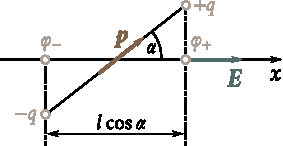
\includegraphics[scale=1]{figures/ch_01/fig_1_13.pdf}
			\caption[]{}
			\label{fig:1_13}
		\end{center}
	\end{minipage}
	\hspace{-0.05cm}
	\begin{minipage}[t]{0.5\linewidth}
		\begin{center}
			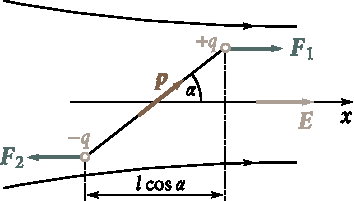
\includegraphics[scale=1]{figures/ch_01/fig_1_14.pdf}
			\caption[]{}
			\label{fig:1_14}
		\end{center}
	\end{minipage}
\vspace{-0.4cm}
\end{figure}

\noindent
Introducing this value into \eqn{1_59}, we find that
\begin{equation}\label{eq:1_60}
	\ab{W}{p} = - q E l \cos\alpha = - p E \cos\alpha.
\end{equation}

\noindent
Here $\alpha$ is the angle between the vectors $\vec{p}$ and $\vec{E}$. We can therefore write \eqn{1_60} in the form
\begin{equation}\label{eq:1_61}
	\ab{W}{p} = - \vecdot{p}{E}.
\end{equation}

\noindent
We must note that this expression takes no account of the energy of interaction of the charges $+q$ and $-q$ forming a dipole.

We have obtained \eqn{1_61} assuming for simplicity's sake that the field is homogeneous. This equation also holds, however, for an inhomogeneous field.

Let us consider a dipole in an inhomogeneous field that is symmetrical relative to the $x$-axis\footnote{A particular case of such a field is that of a point charge if we take a straight line passing through the charge as the $x$-axis.}. Let the centre of the dipole be on this axis, the dipole electric moment making with the axis an angle $\alpha$, differing from $\pi/2$ (\fig{1_14}). In this case, the forces acting on the dipole charges are not identical in magnitude. Therefore, apart from
the rotational moment (torque), the dipole will experience a force tending to move it in the direction of the $x$-axis. To find the value of this force, we shall use \eqn{1_40}, according to which
\begin{equation*}
	F_x = -\diffpartial{\ab{W}{p}}{x},\quad F_y = -\diffpartial{\ab{W}{p}}{y},\quad F_z = -\diffpartial{\ab{W}{p}}{z}.
\end{equation*}

\noindent
In view of \eqn{1_60}, we can written
\begin{equation*}
	\ab{W}{p}(x,y,z) = -p E(x,y,z)\cos\alpha
\end{equation*}

\noindent
(we consider the orientation of the dipole relative to the vector $\vec{E}$ to be constant, $\alpha=\text{constant}$).

For points on the $x$-axis, the derivatives of $E$ with respect to $y$ and $z$ are zero. Accordingly, $\diffinpartial{\ab{W}{p}}{y}=\diffinpartial{\ab{W}{p}}{z}=0$. Thus, only
the force component $F_x$ differs from zero. It is
\begin{equation}\label{eq:1_62}
	F_x = - \diffpartial{\ab{W}{p}}{x} = p \diffpartial{E}{x} \cos\alpha.
\end{equation}

\noindent
This result can be obtained if we take account of the fact that the field strength at the points where the charges $+q$ and $-q$ are (see
\fig{1_14}) differs by the amount $(\diffinpartial{E}{x})l\cos\alpha$. Accordingly, the difference between the forces acting on the charges is $q(\diffinpartial{E}{x})l\cos\alpha$, which coincides with \eqn{1_62}.

When $\alpha$ is less than $\pi/2$, the value of $F_x$ determined by \eqn{1_62} is positive. This signifies that under the action of the force the dipole is pulled into the region of a stronger field (see \fig{1_14}). When $\alpha$ is greater than $\pi/2$, the dipole is pushed out of the field.

\begin{figure}[t]
	\begin{center}
		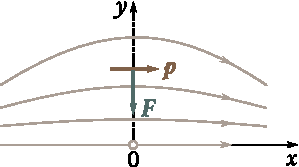
\includegraphics[scale=1]{figures/ch_01/fig_1_15.pdf}
		\caption[]{}
		\label{fig:1_15}
	\end{center}
	\vspace{-0.8cm}
\end{figure}

In the case shown in \fig{1_15}, only the derivative $\diffinpartial{E}{y}$ differs from zero for points on the $y$-axis. Therefore, the force acting on the dipole is determined by the component
\begin{equation*}
	F_y = -\diffpartial{\ab{W}{p}}{y} = p \diffpartial{E}{y},\quad (\cos\alpha=1).
\end{equation*}

\noindent
The derivative $\diffinpartial{E}{y}$ is negative. Consequently, the force is directed as shown in the figure. Thus, in this case too, the dipole is pulled into the field.

We shall note that like $-\diffinpartial{\ab{W}{p}}{x}$ gives the projection of the force acting on the system onto the $x$-axis, so does the derivative of \eqn{1_60} with respect to $\alpha$ taken with the opposite sign give the projection of the torque onto the $\alpha$-``axis'': $T_{\alpha}=-pE\sin\alpha$. The minus sign was obtained because the $\alpha$-``axis'' and the torque $T$ are directed oppositely (see \fig{1_12}).

\section{Field of a System of Charges at Great Distances}\label{sec:1_10}

Let us take a system of $N$ charges $q_1, q_2, \ldots, q_N$ in a volume having linear dimensions of the order of $l$, and study the field set up by this system at distances $r$ that are great in comparison with $l$ ($r>l$). We take the origin of coordinates $0$ inside the volume occupied by the system and shall determine the positions of the charges with the aid of the position vectors $\vec{r}_i$, (\fig{1_16}; to simplify the figure, we have shown only the position vector of the $i$-th charge).

\begin{figure}[t]
	\begin{center}
		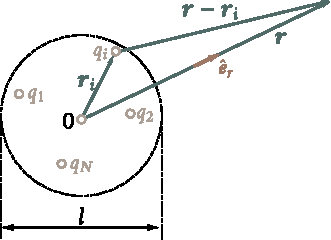
\includegraphics[scale=0.95]{figures/ch_01/fig_1_16.pdf}
		\caption[]{}
		\label{fig:1_16}
	\end{center}
	\vspace{-1.0cm}
\end{figure}

The potential at the point determined by the position vector $\vec{r}$ is
\begin{equation}\label{eq:1_63}
	\varphi(\vec{r}) = \frac{1}{4\pi\varepsilon_0} \sum_{i=1}^N \frac{q_i}{\absolute{\vec{r} - \vec{r}_i}}.
\end{equation}

\noindent
Owing to the smallness of $r_i$ in comparison with $r$, we can assume that
\begin{equation*}
	\absolute{\vec{r} - \vec{r}_i} = r - \vec{r}_i\!\vec{\cdot}\!\vecuni{r} = r\parenthesis{1 - \frac{\vec{r}_i\!\vec{\cdot}\!\vecuni{r}}{r}}
\end{equation*}

\noindent
[compare with Eqs. \eqref{eq:1_47}]. Introduction of this expression into
\eqn{1_63} yields
\begin{equation}\label{eq:1_64}
	\varphi(\vec{r}) = \frac{1}{4\pi\varepsilon_0} \sum_{i=1}^N \frac{q_i}{r} \bracket{\frac{1}{1 - \parenthesis{\vec{r}_i\!\vec{\cdot}\!\vecuni{r}/r}}}.
\end{equation}

\noindent
Using the formula
\begin{equation*}
	\frac{1}{1-x} \approx 1 + x
\end{equation*}

\noindent
which holds when $x\ll 1$, we can transform \eqn{1_64} as follows:
\begin{align}
	\varphi(\vec{r}) &= \frac{1}{4\pi\varepsilon_0} \sum_{i=1}^N \frac{q_i}{r} \parenthesis{1 + \frac{\vec{r}_i\!\vec{\cdot}\!\vecuni{r}}{r}}\nonumber\\
	&= \frac{1}{4\pi\varepsilon_0} \frac{1}{r} \sum_{i=1}^N q_i + \frac{1}{4\pi\varepsilon_0} \frac{1}{r^2} \parenthesis{\sum_{i=1}^N q_i \vec{r}_i}\!\vec{\cdot}\!\vecuni{r}. \label{eq:1_65}
\end{align}

\noindent
The first term of the expression obtained is the potential of the field of a point charge having the value $q=\sum_iq_i$ [compare with \eqn{1_26}]. The second term has the same form as the expression determining the potential of a dipole field, the part of the electric moment of the dipole being played by the quantity
\begin{equation}\label{eq:1_66}
	\vec{p} = \sum_{i=1}^N q_i \vec{r}_i.
\end{equation}

\noindent
This quantity is called the \textbf{dipole electric moment} of a system of charges. It is easy to verify that for a dipole \eqn{1_66} transforms
into the expression $\vec{p}=q\vec{l}$ which we are already familiar with.

\begin{figure}[t]
	\begin{minipage}[t]{0.4\linewidth}
		\begin{center}
			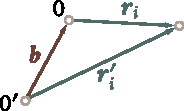
\includegraphics[scale=1]{figures/ch_01/fig_1_17.pdf}
			\caption[]{}
			\label{fig:1_17}
		\end{center}
	\end{minipage}
	\hspace{-0.05cm}
	\begin{minipage}[t]{0.6\linewidth}
		\begin{center}
			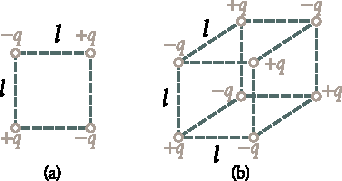
\includegraphics[scale=1]{figures/ch_01/fig_1_18.pdf}
			\caption[]{}
			\label{fig:1_18}
		\end{center}
	\end{minipage}
\vspace{-0.4cm}
\end{figure}

If the total charge of a system is zero ($\sum_iq_i=0$), the value of the dipole moment does not depend on our choice of the origin of coordinates. To convince ourselves that this is true, let us take two arbitrary origins of coordinates $0$ and $0'$ (\fig{1_17}). The position vectors of the $i$-th charge conducted from these points are related as follows:
\begin{equation}\label{eq:1_67}
	\vec{r}_i' = \vec{b} + \vec{r}_i
\end{equation}

\noindent
(what the vector $\vec{b}$ is clear from the figure). With account taken of \eqn{1_67}, the dipole moment in the system with the origin $0'$ is
\begin{equation*}
	\vec{p}' = \sum_i q_i \vec{r}_i = \sum_i q_i (\vec{b} + \vec{r}_i) = \vec{b} \sum_i q_i + \sum_i q_i \vec{r}_i.
\end{equation*}

\noindent
The first addend equals zero (because $\sum_iq_i=0$). The second one is $\vec{p}$---the dipole moment in a coordinate system with its origin at $0$. We have thus obtained that $\vec{p}'=\vec{p}$.

Equation \eqref{eq:1_65} is in essence the first two terms of the series expansion of function \eqref{eq:1_63} by powers of $r_i/r$. When $\sum_iq_i\neq 0$, the first term of \eqn{1_65} makes the main contribution to the potential (the second term diminishes in proportion to $1/r^2$ and is therefore much smaller than the first one). For an electrically neutral system ($\sum_iq_i=0$), the first term equals zero, and the potential is determined mainly by the second term of \eqn{1_65}. This is how matters stand, in particular, for the field of a dipole.

For the system of charges depicted in \fig{1_18}a and called a \textbf{quadrupole}, both $\sum_iq_i$ and $\vec{p}$ equal zero so that \eqn{1_65} gives a zero value of the potential. Actually, however, the field of a quadrupole, although it is much weaker than that of a dipole (with the same values of $q$ and $l$), differs from zero. The potential of the field set up by a quadrupole is determined mainly by the third term of the expansion that is proportional to $1/r^3$. To obtain this term, we must take into consideration quantities of the order of $(r_i/r)^2$ which we disregarded in deriving \eqn{1_65}. For the system of charges shown in \fig{1_18}b and called an \textbf{octupole}, the third term of the expansion also equals zero. The potential of the field of such a system is determined by the fourth term of the expansion, which is proportional to $1/r^4$.

It must be noted that the quantity equal to $\sum_iq_i$ in the numerator of the first term of \eqn{1_65} is called a \textbf{monopole} or a \textbf{zero-order multipole}, a dipole is also called a \textbf{first-order multipole}, a quadrupole is called a \textbf{second-order multipole}, and so on.

Thus, in the general case, the field of a system of charges at great distances can be represented as the superposition of fields set up by multipoles of different orders---a monopole, dipole, quadrupole, octupole, etc.

\section{A Description of the Properties of Vector Fields}\label{sec:1_11}

To continue our study of the electric field, we must acquaint ourselves with the mathematical tools used to describe the properties of vector fields. These tools are called \textbf{vector analysis}. In the present section, we shall treat the fundamental concepts and selected formulas of vector analysis, and also prove its two main theorems---the Ostrogradsky-Gauss theorem (sometimes called Gauss's divergence theorem) and Stokes's theorem.

The quantities used in vector analysis can be best illustrated for the field of the velocity vector of a flowing liquid. We shall therefore introduce these quantities while dealing with the flow of an ideal incompressible liquid, and then extend the results obtained to vector fields of any nature.

We are already acquainted with one of the concepts of vector analysis. This is the \textbf{gradient}, used to characterize scalar fields. If the value of the scalar quantity $\varphi=\varphi(x, y, z)$ is compared with every point P having the coordinates $x, y, z$, we say that the scalar field of $\varphi$ has been set. The gradient of the quantity $\varphi$ is defined as the vector
\begin{equation}\label{eq:1_68}
	\grad{\varphi} = \diffpartial{\varphi}{x}\,\vecuni{x} + \diffpartial{\varphi}{y}\,\vecuni{y} + \diffpartial{\varphi}{z}\,\vecuni{z}.
\end{equation}

The increment of the function $\varphi$ upon displacement over the length $\deriv{\vec{l}}=\vecuni{x}\,\deriv{x}+\vecuni{y}\,\deriv{y}+\vecuni{z}\,\deriv{z}$ is
\begin{equation*}
	\deriv{\varphi} = \diffpartial{\varphi}{x}\,\deriv{x} + \diffpartial{\varphi}{y}\,\deriv{y} + \diffpartial{\varphi}{z}\,\deriv{z}
\end{equation*}

\noindent
which can be written in the form
\begin{equation}\label{eq:1_69}
	\deriv{\varphi} = \grad{\varphi} \ccdot \deriv{\vec{l}}.
\end{equation}

Now we shall go over to establishing the characteristics of vector fields.

\begin{figure}[t]
	\begin{center}
		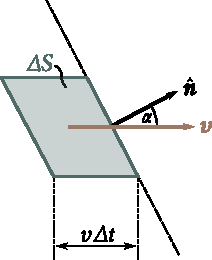
\includegraphics[scale=1]{figures/ch_01/fig_1_19.pdf}
		\caption[]{}
		\label{fig:1_19}
	\end{center}
	\vspace{-0.8cm}
\end{figure}

\textbf{Vector flux.} Assume that the flow of a liquid is characterized by the field of the velocity vector. The volume of liquid flowing in unit time through an imaginary surface $S$ is called the flux of the liquid through this surface. To find the flux, let us divide the surface into elementary sections of the size $\Delta{S}$. It can be seen from \fig{1_19} that during the time $\Delta{t}$ a volume of liquid equal to
\begin{equation*}
	\Delta{V} = (\Delta{S}\cos\alpha) v\Delta{t}
\end{equation*}

\noindent
will pass through section $\Delta{S}$. Dividing this volume by the time $\Delta{t}$, we shall find the flux through surface $\Delta{S}$:
\begin{equation*}
	\Delta{\Phi} = \frac{\Delta{V}}{\Delta{t}} = \Delta{S} v \cos\alpha.
\end{equation*}

\noindent
Passing over to differentials, we find that
\begin{equation}\label{eq:1_70}
	\deriv{\Phi} = (v \cos\alpha)\, \deriv{S}.
\end{equation}

\noindent
Equation \eqref{eq:1_70} can be written in two other ways. First, if we take into account that $v\cos\alpha$ gives the projection of the velocity vector onto the normal $\vecuni{n}$ to area $\deriv{S}$, we can write \eqn{1_70} in the form
\begin{equation}\label{eq:1_71}
	\deriv{\Phi} = v_n\, \deriv{S}.
\end{equation}

\noindent
Second, we can introduce the vector $\deriv{\vec{S}}$ whose magnitude equals that of area $\deriv{S}$, while its direction coincides with the direction of a normal $\hatvec{n}$ to the area:
\begin{equation*}
	\deriv{\vec{S}} = \deriv{S}\, \hatvec{n}.
\end{equation*}

\noindent
Since the direction of the vector $\hatvec{n}$ is chosen arbitrarily (it can be directed to either side of the area), then $\deriv{\vec{S}}$ is not a true vector, but is a pseudo vector. The angle $\alpha$ in \eqn{1_70} is the angle between the vectors $\vec{v}$ and $\deriv{\vec{S}}$. Hence, this equation can be written in the form
\begin{equation}\label{eq:1_72}
	\deriv{\Phi} = \vec{v} \ccdot \deriv{\vec{S}}.
\end{equation}

By summating the fluxes through all the elementary areas into which we have divided surface $S$, we get the flux of the liquid through $S$:
\begin{equation}\label{eq:1_73}
	\Phi_v = \int_S \vec{v} \ccdot \deriv{\vec{S}} = \int_S v_n\, \deriv{S}.
\end{equation}

\noindent
A similar expression written for an arbitrary vector field $\vec{a}$, \ie, the quantity
\begin{equation}\label{eq:1_74}
	\Phi_a = \int_S \vec{a} \ccdot \deriv{\vec{S}} = \int_S a_n\, \deriv{S}
\end{equation}

\noindent
is called the \textbf{flux of the vector a through surface} $S$. In accordance with this definition, the flux of a liquid can be called the flux of the vector $\vec{v}$ through the relevant surface [see \eqn{1_73}].

The flux of a vector is an algebraic quantity. Its sign depends on the choice of the direction of a normal to the elementary areas into which surface $S$ is divided in calculating the flux. Reversal of the direction of the normal changes the sign of $a_n$ and, therefore, the sign of the quantity \eqref{eq:1_74}. The customary practice for closed surfaces is calculation of the flux ``emerging outward'' from the region enclosed by the surface. Accordingly, in the following we shall always implicate that $\hatvec{v}$ is an outward normal.

\begin{figure}[t]
	\begin{center}
		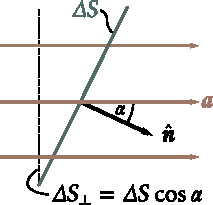
\includegraphics[scale=0.95]{figures/ch_01/fig_1_20.pdf}
		\caption[]{}
		\label{fig:1_20}
	\end{center}
	\vspace{-1.0cm}
\end{figure}

We can give an illustrative geometrical interpretation of the vector flux. For this purpose, we shall represent a vector field by a system of
lines $\vec{a}$ constructed so that the density of the lines at every point is numerically equal to the magnitude of the vector $\vec{a}$ at the same point of the field (compare with the rule for constructing the lines of the vector $\vec{E}$ set out at the end of \sect{1_5}). Let us find the number $\Delta{N}$ of intersections of the field lines with the imaginary area $\Delta{S}$. A glance at \fig{1_20} shows that this number equals the density of the lines (\ie, $a$) multiplied by $\Delta{S}_{\perp}=\Delta{S}\cos\alpha$:
\begin{equation*}
	\Delta{N}\, (=)\, a \Delta{S}\cos\alpha = a_n \Delta{S}.
\end{equation*}

\noindent
We are speaking only about the numerical equality between $\Delta{N}$ and $a_n\Delta{S}$. This is why the equality sign is confined in parentheses. According to \eqn{1_74}, the expression $a_n\Delta{S}$ is $\Delta{\Phi}$---the flux of the vector a through area $\Delta{S}$. Thus,
\begin{equation}\label{eq:1_75}
	\Delta{N}\, (=)\, \Delta{\Phi}_a.
\end{equation}

For the sign of $\Delta{N}$ to coincide with that of $\Delta{\Phi}_a$, we must consider those intersections to be positive for which the angle $\alpha$ between the positive direction of a field line and a normal to the area is acute. The intersection should be considered negative if the angle $\alpha$ is obtuse. For the area shown in \fig{1_20}, all three intersections are positive: $\Delta{N}=+3$ ($\Delta{\Phi}_a$ in this case is also positive because $a_n>0$). If the direction of the normal in \fig{1_20} is reversed, the intersections will become negative ($\Delta{N}=-3$), and the flux $\Delta{\Phi}_a$ will also be negative.

Summation of \eqn{1_75} over the finite imaginary surface $S$ yields
\begin{equation}\label{eq:1_76}
	\Delta{\Phi}_a\, (=)\, \sum\Delta{N} = N_+ - N_-
\end{equation}

\noindent
where $N_+$ and $N_-$ are the total number of positive and negative intersections of the field lines with surface $S$, respectively.

The reader may be puzzled by the circumstance that since the flux, as a rule, is expressed by a fractional number, the number of intersections of the field lines with a surface compared with the flux will also be fractional. Do not be confused by this, however. Field lines are a purely conditional image deprived of a physical meaning.

Let us take an imaginary surface in the form of a strip of paper whose bottom part is twisted relative to the top one through the angle $\pi$ (\fig{1_21}). The direction of a normal must be chosen identically for the entire surface. Hence, if in the top part of the strip a positive normal is directed to the right, then in the bottom part a normal will be directed to the left. Accordingly, the intersections of the field lines depicted in \fig{1_21} with the top half of the surface must be considered positive, and with the bottom half, negative.

\begin{figure}[t]
	\begin{minipage}[t]{0.4\linewidth}
		\begin{center}
			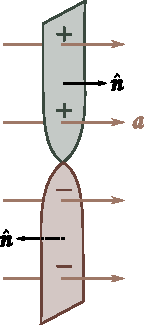
\includegraphics[scale=0.95]{figures/ch_01/fig_1_21.pdf}
			\caption[]{}
			\label{fig:1_21}
		\end{center}
	\end{minipage}
	\hspace{-0.05cm}
	\begin{minipage}[t]{0.6\linewidth}
		\begin{center}
			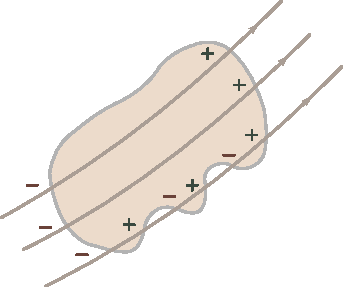
\includegraphics[scale=0.95]{figures/ch_01/fig_1_22.pdf}
			\caption[]{}
			\label{fig:1_22}
		\end{center}
	\end{minipage}
\vspace{-0.4cm}
\end{figure}

An outward normal is considered to be positive for a closed surface (\fig{1_22}). Therefore, the intersections corresponding to outward protrusion of the lines (in this case the angle $\alpha$ is acute) must be taken with the plus sign, and the ones appearing when the lines enter the surface (in this case the angle $\alpha$ is obtuse) must be taken with the minus sign.

Inspection of \fig{1_22} shows that when the field lines enter a closed surface continuously, each line when intersecting the surface enters it and emerges from it the same number of times. As a result, the flux of the corresponding vector through this surface equals zero. It is easy to see that if field lines end inside a surface, the vector flux through the closed surface will numerically equal the difference between the number of lines beginning inside the surface ($\ab{N}{beg}$) and the number of lines terminating inside the surface ($\ab{N}{term}$):
\begin{equation}\label{eq:1_77}
	\Phi_a\, (=)\, \ab{N}{beg} - \ab{N}{term}.
\end{equation}

\noindent
The sign of the flux depends on which of these numbers is greater. When $\ab{N}{beg}$ is equal to $\ab{N}{term}$, the flux equals zero.

\textbf{Divergence.} Assume that we are given the field of the velocity vector of an incompressible continuous liquid. Let us take an imaginary closed surface $S$ in the vicinity of point P (\fig{1_23}). If in the volume confined by this surface no liquid appears and no liquid vanishes, then the flux flowing outward through the surface will evidently equal zero. A liquid flux $\Phi_v$ other than zero will indicate that there are liquid sources or sinks inside the surface, \ie, points at which the liquid enters the volume (sources) or emerges from it (sinks). The magnitude of the flux determines the total algebraic power of the sources and sinks\footnote{The power of a source (sink) is defined as the volume of liquid discharged (absorbed) in unit time. A sink can be considered as a source with a negative power.}. When the sources predominate over the sinks, the magnitude of the flux will be positive, and when the sinks predominate, negative.

\begin{figure}[t]
	\begin{center}
		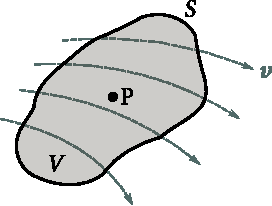
\includegraphics[scale=1]{figures/ch_01/fig_1_23.pdf}
		\caption[]{}
		\label{fig:1_23}
	\end{center}
	\vspace{-0.8cm}
\end{figure}

The quotient obtained when dividing the flux $\Phi_v$ by the volume which it flows out from, \ie,
\begin{equation}\label{eq:1_78}
	\frac{\Phi_v}{V}
\end{equation}

\noindent
gives the average unit power of the sources confined in the volume $V$. In the limit when $V$ tends to zero, \ie, when the volume $V$ contracts to point P, expression \eqref{eq:1_78} gives the true unit power of the sources at point P, which is called the \textbf{divergence} of the vector $\vec{v}$ (it is designated by $\diverg{\vec{v}}$). Thus, by definition,
\begin{equation*}
	\diverg{\vec{v}} = \lim_{V\to \text{P}} \frac{\Phi_v}{V}.
\end{equation*}

\noindent
The divergence of any vector $\vec{a}$ is determined in a similar way:
\begin{equation}\label{eq:1_79}
	\diverg{\vec{a}} = \lim_{V\to \text{P}} \frac{\Phi_v}{V} = \lim_{V\to \text{P}} \oint \vec{a} \ccdot \deriv{\vec{S}}.
\end{equation}

\noindent
The integral is taken over arbitrary closed surface $S$ surrounding point P\footnote{The circle on the integral sign signifies that integration is performed over a closed surface.}; $V$ is the volume confined by this surface. Since the transition $V\to$P is being performed upon which $S$ tends to zero, we can assume that \eqn{1_79} cannot depend on the shape of the surface. This assumption is confirmed by strict calculations.

Let us surround point P with a spherical surface of an extremely small radius $r$ (\fig{1_24}). Owing to the smallness of $r$, the volume $V$ enclosed by the sphere will also be very small. We can therefore consider with a high degree of accuracy that the value of $\diverg{\vec{a}}$ within the limits of the volume $V$ is constant\footnote{It is assumed that the value of $\diverg{\vec{a}}$ changes continuously, without any jumps, when passing from one point of a field to another.}. In this case, we can write in accordance with \eqn{1_79} that
\begin{equation*}
	\Phi_a \approx (\diverg{\vec{a}}) V
\end{equation*}

\noindent
where $\Phi_a$ is the flux of the vector a through the surface surrounding the volume $V$. By \eqn{1_77}, $\Phi_a$ equals $\ab{N}{beg}$, the number of lines of a beginning inside $V$ if $\diverg{\vec{a}}$ at point P is positive, or $\ab{N}{term}$, the number of lines of a terminating inside $V$ if $\diverg{\vec{a}}$ at point P is negative.

It follows from the above that the lines of the vector $\vec{a}$ begin in the closest vicinity of a point with a positive divergence. The field lines ``diverge'' from this point; the latter is the ``source'' of the field (\fig{1_24}a). On the other hand, in the vicinity of a point with a negative divergence, the lines of the vector $\vec{a}$ terminate. The field lines ``converge'' toward this point; the latter is the ``sink'' of the field (\fig{1_24}b). The greater the absolute value of $\diverg{\vec{a}}$, the bigger is the number of lines that begin or terminate in the vicinity of the given point.

It can be seen from definition \eqref{eq:1_79} that the divergence is a scalar function of the coordinates determining the positions of points in space (briefly---a point function). Definition \eqref{eq:1_79} is the most general one that is independent of the kind of coordinate system used.

\begin{figure}[t]
	\begin{minipage}[t]{0.5\linewidth}
		\begin{center}
			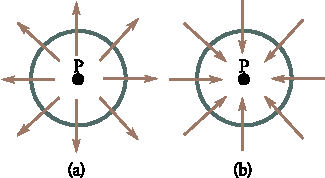
\includegraphics[scale=1.0]{figures/ch_01/fig_1_24.pdf}
			\caption[]{}
			\label{fig:1_24}
		\end{center}
	\end{minipage}
	\hspace{-0.05cm}
	\begin{minipage}[t]{0.5\linewidth}
		\begin{center}
			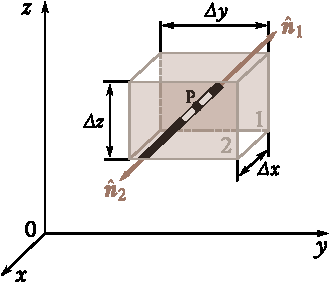
\includegraphics[scale=1.0]{figures/ch_01/fig_1_25.pdf}
			\caption[]{}
			\label{fig:1_25}
		\end{center}
	\end{minipage}
\vspace{-0.4cm}
\end{figure}

Let us find an expression for the divergence in a Cartesian coordinate system. We shall consider a small volume in the form of a parallelepiped with ribs parallel to the coordinate axes in the vicinity of point $P(x, y, z)$ (\fig{1_25}). The vector flux through the surface of the parallelepiped is formed from the fluxes passing through each of the six faces separately.

Let us find the flux through the pair of faces perpendicular to the $x$-axis (in \fig{1_25} these faces are designated by shaded areas and by the numbers 1 and 2). The outward normal $\hatvec{n}_2$ to face 2 coincides with the direction of the $x$-axis. Hence, for points of this face, $a_{n_2}=a_x$. The outward normal $\hatvec{n}_1$ to face 1 is directed oppositely to the $x$-axis. Therefore, for points on this face, $a_{n_2}=-a_x$. The flux through face 2 can be written in the form
\begin{equation*}
	a_{x,2}\Delta{y}\Delta{z}
\end{equation*}

\noindent
where $a_{x,2}$ is the value of $a_x$ averaged over face 2. The flux through face 1 is
\begin{equation*}
	- a_{x,1}\Delta{y}\Delta{z}
\end{equation*}

\noindent
where $a_{x,1}$ is the average value of $a_x$ for face 1. The total flux through faces 1 and 2 is determined by the expression
\begin{equation}\label{eq:1_80}
	(a_{x,2} - a_{x,1}) \Delta{y}\Delta{z}.
\end{equation}

The difference $a_{x,2}-a_{x,1}$ is the increment of the average (over a face) value of $a_x$ upon a displacement along the $x$-axis by $\Delta{x}$. Owing to the smallness of the parallelepiped (we remind our reader that we shall let its dimensions shrink to zero), this increment can be written in the form $(\diffinpartial{a_x}{x})\Delta{x}$, where the value $\diffinpartial{a_x}{x}$ is taken at point P\footnote{The inaccuracy which we tolerate here vanishes when the volume shrinks to point P in the limit transition.}. Therefore, \eqn{1_80} becomes
\begin{equation*}
	\diffpartial{a_x}{x}\Delta{x}\Delta{y}\Delta{z} = \diffpartial{a_x}{x}\Delta{V}.
\end{equation*}

\noindent
Similar reasoning allows us to obtain the following expressions for the fluxes through the pairs of faces perpendicular to the $y$- and $z$-axes:
\begin{equation*}
	\diffpartial{a_y}{y}\Delta{x}\Delta{y}\Delta{z} = \diffpartial{a_y}{y}\Delta{V},\quad \diffpartial{a_z}{z}\Delta{x}\Delta{y}\Delta{z} = \diffpartial{a_z}{z}\Delta{V}.
\end{equation*}

Thus, the total flux through the entire close surface is determined by the expression
\begin{equation*}
	\Phi_a = \parenthesis{\diffpartial{a_x}{x} + \diffpartial{a_y}{y} + \diffpartial{a_z}{z}}\Delta{V}.
\end{equation*}

\noindent
Dividing this expression by $\Delta{V}$, we shall find the divergence of the vector a at point $P(x, y, z)$:
\begin{equation}\label{eq:1_81}
	\diverg{\vec{a}} = \diffpartial{a_x}{x} + \diffpartial{a_y}{y} + \diffpartial{a_z}{z}.
\end{equation}

\textbf{The Ostrogradsky-Gauss Theorem.} If we know the divergence of the vector $\vec{a}$ at every point of space, we can calculate the flux of this vector through any closed surface of finite dimensions. Let us first do this for the flux of the vector $\vec{v}$ (a liquid flux). The product of $\diverg{\vec{v}}$ and $\deriv{V}$ gives the power of the sources of the liquid confined within the volume $\deriv{V}$. The sum of such products, \ie, $\int(\diverg{\vec{v}})\,\deriv{V}$, gives the total algebraic power of the sources confined in the volume $V$ over which integration is performed. Owing to incompressibility of the liquid, the total power of the sources must equal the liquid flux emerging through surface $S$ enclosing the volume $V$. We thus arrive at the equation
\begin{equation*}
	\oint_S \vec{v} \ccdot \deriv{\vec{S}} = \int_V (\diverg{\vec{v}})\,\deriv{V}.
\end{equation*}

\noindent
A similar equation holds for a vector field of any nature:
\begin{equation}\label{eq:1_82}
	\oint_S \vec{a} \ccdot \deriv{\vec{S}} = \int_V (\diverg{\vec{a}})\,\deriv{V}.
\end{equation}

\noindent
This relation is called the \textbf{Ostrogradsky-Gauss} theorem. The integral in the left-hand side of the equation is calculated over an arbitrary closed surface $S$, and the integral in the right-hand side over the volume $V$ enclosed by this surface.

\textbf{Circulation.} Let us revert to the flow of an ideal incompressible liquid. Imagine a closed line---the contour $\Gamma$. Assume that in some way or other we have instantaneously frozen the
liquid in the entire volume except for a very thin closed channel of constant cross section including the contour $\Gamma$ (\fig{1_26}). Depending on the nature of the velocity vector field, the liquid in the channel formed will either be stationary or move along the contour (circulate) in one of the two possible directions. Let us take the quantity equal to the product of the velocity of the liquid in the channel and the length of the contour $l$ as a measure of this motion. This quantity is called the \textbf{circulation} of the vector $\vec{v}$ around the contour $\Gamma$. Thus,
\begin{equation*}
	\text{circulation of $\vec{v}$ around $\Gamma$} = vl
\end{equation*}

\noindent
(since we assumed that the channel has a constant cross section, the magnitude of the velocity, $v$, is a constant).

\begin{figure}[t]
	\begin{center}
		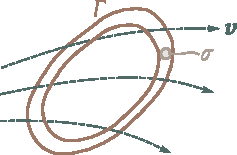
\includegraphics[scale=1]{figures/ch_01/fig_1_26.pdf}
		\caption[]{}
		\label{fig:1_26}
	\end{center}
	\vspace{-0.8cm}
\end{figure}

At the moment when the walls freeze, the velocity component perpendicular to a wall will be eliminated in each of the liquid particles, and only the velocity component tangent to the contour will remain, \ie, $v_l$. The momentum $\deriv{\vec{p}_l}$, is associated with this component. The magnitude of the momentum for a liquid particle contained within a segment of the channel of length $\deriv{l}$ is $\rho\sigma v_l\,\deriv{l}$ ($\rho$ is the density of the liquid, and $\sigma$ is the cross-sectional area of the channel). Since the liquid is ideal, the action of the walls can change only the direction of the vector $\deriv{\vec{p}_l}$, but not its magnitude. The interaction between the liquid particles will cause a redistribution of the momentum between them that will level out the velocities of all the particles. The algebraic sum of the tangential components of the momenta cannot change: the momentum acquired by one of the interacting particles equals the momentum lost by the second particle. This signifies that
\begin{equation*}
	\rho\sigma vl = \oint_{\Gamma} \rho \sigma v_l\,\deriv{l}
\end{equation*}

\noindent
where $v$ is the circulation velocity, and $v_l$ is the tangential component of the liquid's velocity in the volume $\sigma\,\deriv{l}$ at the moment of time preceding the freezing of the channel walls. Cancelling $\rho\sigma$, we get
\begin{equation*}
	\text{circulation of $\vec{v}$ around $\Gamma$} = vl = \oint_{\Gamma} v_l\,\deriv{l}.
\end{equation*}

\noindent
The circulation of any vector $\vec{a}$ around an arbitrary closed contour $\Gamma$ is determined in a similar way:
\begin{equation}\label{eq:1_83}
	\text{circulation of $\vec{a}$ around $\Gamma$} = \oint_{\Gamma} \vec{a} \ccdot \deriv{\vec{l}} = \oint_{\Gamma} a_l\,\deriv{l}.
\end{equation}

It may seem that for the circulation to be other than zero the vector lines must be closed or at least bent in some way or other in the direction of circumventing the contour. It is easy to see that this assumption is wrong. Let us consider the laminar flow of water in a river. The velocity of the water directly at the river bottom is zero and grows as we approach the surface of the water (\fig{1_27}). The streamlines (lines of the vector $\vec{v}$) are straight. Notwithstanding this fact, the circulation of the vector $\vec{v}$ around the contour depicted by the dash line obviously differs from zero. On the other hand, in a field with curved lines, the circulation may equal zero.

\begin{figure}[t]
	\begin{minipage}[t]{0.5\linewidth}
		\begin{center}
			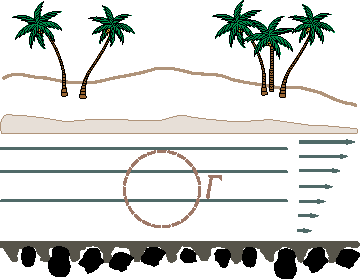
\includegraphics[scale=0.95]{figures/ch_01/fig_1_27.pdf}
			\caption[]{}
			\label{fig:1_27}
		\end{center}
	\end{minipage}
	\hspace{-0.05cm}
	\begin{minipage}[t]{0.5\linewidth}
		\begin{center}
			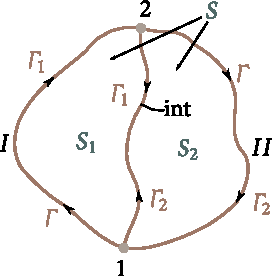
\includegraphics[scale=0.95]{figures/ch_01/fig_1_28.pdf}
			\caption[]{}
			\label{fig:1_28}
		\end{center}
	\end{minipage}
\vspace{-0.6cm}
\end{figure}

Circulation has the property of additivity. This signifies that the sum of the circulations around contours $\Gamma_1$ and $\Gamma_2$ enclosing neighboring surfaces $S_1$ and $S_2$ (\fig{1_28}) equals the circulation around contour $\Gamma$ enclosing surface $S$, which is the sum of surfaces $S_1$ and $S_2$. Indeed, the circulation $C_1$ around the contour bounding surface $S_1$ can be represented as the sum of the integrals
\begin{equation}\label{eq:1_84}
	C_1 = \oint_{\Gamma_1} \vec{a} \ccdot \deriv{\vec{l}} = \int_{1,(I)}^2 \vec{a} \ccdot \deriv{\vec{l}} + \int_{2,(\text{int.})}^1 \vec{a} \ccdot \deriv{\vec{l}}.
\end{equation}

\noindent
The first integral is taken over section $I$ of the outer contour, the second over the interface between surfaces $S_1$ and $S_2$ in direction $2$-$1$.

Similarly, the circulation $C_2$ around the contour enclosing surface $S_2$ is
\begin{equation}\label{eq:1_85}
	C_2 = \oint_{\Gamma_2} \vec{a} \ccdot \deriv{\vec{l}} = \int_{2,(II)}^1 \vec{a} \ccdot \deriv{\vec{l}} + \int_{1,(\text{int.})}^2 \vec{a} \ccdot \deriv{\vec{l}}.
\end{equation}

\noindent
The first integral is taken over section $II$ of the outer contour, the second over the interface between surfaces $S_1$ and $S_2$ in direction $1$-$2$.

The circulation around the contour bounding total surface $S$ can be represented in the form
\begin{equation}\label{eq:1_86}
	C = \oint_{\Gamma} \vec{a} \ccdot \deriv{\vec{l}} = \int_{1,(I)}^2 \vec{a} \ccdot \deriv{\vec{l}} + \int_{2,(II)}^1 \vec{a} \ccdot \deriv{\vec{l}}.
\end{equation}

\noindent
The second addends in Eqs. \eqref{eq:1_84} and \eqref{eq:1_85} differ only in their sign. Therefore, the sum of these expressions will equal \eqn{1_86}. Thus,
\begin{equation}\label{eq:1_87}
	C = C_1 + C_2.
\end{equation}

Equation \eqref{eq:1_87} which we have proved does not depend on the shape of the surfaces and holds for any number of addends. Hence, if we divide an arbitrary open surface $S$ into a great number of elementary surfaces $\Delta{S}$\footnote{In the figure, the elementary surfaces are depicted in the form of rectangles. Actually, their shape may be absolutely arbitrary.} (\fig{1_29}), then the circulation around the contour enclosing $S$ can be written as the sum of the elementary circulations $\Delta{C}$ around the contours enclosing the $\Delta{S}$'s:
\begin{equation}\label{eq:1_88}
	C = \sum_i \Delta{C}_i.
\end{equation}

\begin{figure}[t]
	\begin{center}
		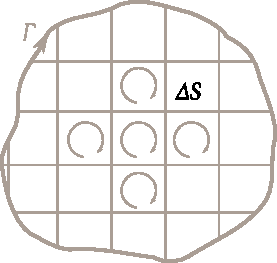
\includegraphics[scale=1]{figures/ch_01/fig_1_29.pdf}
		\caption[]{}
		\label{fig:1_29}
	\end{center}
	\vspace{-0.8cm}
\end{figure}

\textbf{Curl.} The additivity of the circulation permits us to introduce the concept of unit circulation, \ie, consider the ratio of the circulation $C$ to the magnitude of surface $S$ around which the circulation ``flows''. When surface $S$ is finite, the ratio $C/S$ gives the mean value of the unit circulation. This value characterizes the properties of a field averaged over surface $S$. To obtain the characteristic of the field at point P, we must reduce the dimensions of the surface, making it shrink to point P. The ratio $C/S$ tends to a limit that characterizes the properties of the field at point P.

Thus, let us take an imaginary contour $\Gamma$ in a plane passing through point P, and consider the expression
\begin{equation}\label{eq:1_89}
	\lim_{S\to\text{P}} \frac{C_a}{S}
\end{equation}

\noindent
where $C_a$ is the circulation of the vector $\vec{a}$ around the contour $\Gamma$ and $S$ is the surface area enclosed by the contour.

Limit \eqref{eq:1_89} calculated for an arbitrarily oriented plane cannot be an exhaustive characteristic of the field at point P because the magnitude of this limit depends on the orientation of the contour in space in addition to the properties of the field at point P. This orientation can be given by the direction of a positive normal $\hatvec{n}$ to the plane of the contour (a positive normal is one that is associated with the direction of circumvention of the contour in integration by the right-hand screw rule). In determining limit \eqref{eq:1_89} at the same point P for different directions $\hatvec{n}$, we shall obtain different values. For opposite directions, these values will differ only in their sign (reversal of the direction $\hatvec{n}$ is equivalent to reversing the direction of circumvention of the contour in integration, which only causes a change in the sign of the circulation). For a certain direction of the normal, the magnitude of expression \eqref{eq:1_89} at the given point will be maximum.

Thus, quantity \eqref{eq:1_89} behaves like the projection of a vector onto the direction of a normal to the plane of the contour around which the circulation is taken. The maximum value of quantity \eqref{eq:1_89} determines the magnitude of this vector, and the direction of the positive normal $\hatvec{n}$ at which the maximum is reached gives the direction of the vector. This vector is called the \textbf{curl} of the vector $\vec{a}$. lts symbol is $\curl{\vec{a}}$. Using this notation, we can write expression \eqref{eq:1_89} in the form
\begin{equation}\label{eq:1_90}
	(\curl{\vec{a}})_n = \lim_{S\to\text{P}} \frac{C_a}{S} = \lim_{S\to\text{P}} \frac{1}{S} \oint_S \vec{a}\, \deriv{\vec{l}}.
\end{equation}

We can obtain a graphical picture of the curl of the vector $\vec{v}$ by imagining a small and light fan impeller placed at the given point of a flowing liquid (\fig{1_30}). At the spots where the curl differs from zero, the impeller will rotate, its velocity being the higher, the greater in value is the projection of the curl onto the impeller axis.

Equation \eqref{eq:1_90} defines the vector $\curl{\vec{a}}$. This definition is a most general one that does not depend on the kind of coordinate system used. To find expressions for the projections of the vector $\curl{\vec{a}}$ onto the axes of a Cartesian coordinate system, we must determine the values of quantity \eqref{eq:1_90} for such orientations of area $S$ for which the normal $\hatvec{n}$ to the area coincides with one of the axes $x, y, z$. If, for example, we direct $\hatvec{n}$ along the $x$-axis, then \eqref{eq:1_90} becomes $(\curl{\vec{a}})_x$.
Contour $\Gamma$ in this case is arranged in a plane parallel to the coordinate plane $yz$. Let us take this contour in the form of a rectangle with the sides $\Delta{y}$ and $\Delta{z}$ (\fig{1_31}, the $x$-axis is directed toward us in this figure; the direction of circumvention indicated in the figure is associated with the direction of the $x$-axis by the right-hand screw rule). Section $1$ of the contour is opposite in direction to the $z$-axis. Therefore, $a_l$ on this section coincides with $-a_z$. Similar reasoning shows that $a_l$ on sections $2$, $3$, and $4$ equals $a_y$, $a_z$, and $-a_y$, respectively. Hence, the circulation can be written in the form
\begin{equation}\label{eq:1_91}
	\parenthesis{a_{z,3} - a_{z,1}} \Delta{z} - \parenthesis{a_{y,4} - a_{y,2}} \Delta{y}
\end{equation}

\noindent
where $a_{z,3}$ and $a_{z,1}$ are the average values of $a_z$ on sections $3$ and $1$, respectively, and $a_{y,4}$ and $a_{y,2}$ are the average values of $a_{y}$ on sections $4$ and $2$.

\begin{figure}[t]
	\begin{minipage}[t]{0.5\linewidth}
		\begin{center}
			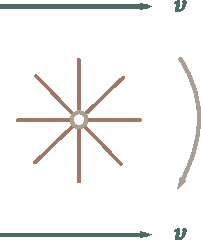
\includegraphics[scale=1]{figures/ch_01/fig_1_30.pdf}
			\caption[]{}
			\label{fig:1_30}
		\end{center}
	\end{minipage}
	\hspace{-0.1cm}
	\begin{minipage}[t]{0.5\linewidth}
		\begin{center}
			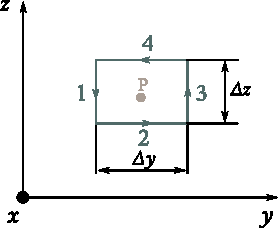
\includegraphics[scale=1]{figures/ch_01/fig_1_31.pdf}
			\caption[]{}
			\label{fig:1_31}
		\end{center}
	\end{minipage}
\vspace{-0.4cm}
\end{figure}

The difference $a_{z,3}-a_{z,1}$ is the increment of the average value of $a_z$ on the section $\Delta{z}$ when this section is displaced in the direction of the $y$-axis by $\Delta{y}$. Owing to the smallness of $\Delta{y}$ and $\Delta{z}$, this increment can be represented in the form $(\diffinpartial{a_z}{y})\Delta{y}$, where the value of $\diffinpartial{a_z}{y}$ is taken for point P\footnote{The inaccuracy which we tolerate here vanishes when the contour shrinks to point P in the limit transition.}. Similarly, the difference $a_{y,4}-a_{y,2}$ can be represented in the form $(\diffinpartial{a_y}{z})\Delta{z}$.
Using these expressions in \eqn{1_91} and putting the common factor outside the parentheses, we get the following expression for the circulation:
\begin{equation*}
	\parenthesis{\diffpartial{a_z}{y} - \diffpartial{a_y}{z}} \Delta{y}\Delta{z} = \parenthesis{\diffpartial{a_z}{y} - \diffpartial{a_y}{z}} \Delta{S}
\end{equation*}

\noindent
where $\Delta{S}$ is the area of the contour. Dividing the circulation by $\Delta{S}$, we find the expression for the projection of $\curl{\vec{a}}$ onto the $x$-axis:
\begin{equation}\label{eq:1_92}
	(\curl{\vec{a}})_x = \diffpartial{a_z}{y} - \diffpartial{a_y}{z}.
\end{equation}

\noindent
We can find by similar reasoning that
\begin{align}
	(\curl{\vec{a}})_y &= \diffpartial{a_x}{z} - \diffpartial{a_z}{x}, \label{eq:1_93}\\
	(\curl{\vec{a}})_z &= \diffpartial{a_y}{x} - \diffpartial{a_x}{y}. \label{eq:1_94}
\end{align}

It is easy to see that any of the equations \eqref{eq:1_92}-\eqref{eq:1_94} can be obtained from the preceding one [\eqn{1_94} should be considered as the preceding one for \eqn{1_94}] by the so-called cyclic transposition of the coordinates, \ie, by replacing the coordinates according to the scheme
\begin{equation*}
	\begin{tikzcd}[column sep=small]
x \arrow[rr, bend left] &           & y \arrow[ld, bend left] \\
                        & z \arrow[lu, bend left] &
\end{tikzcd}
\end{equation*}

Thus, the curl of the vector $\vec{a}$ is determined in the Cartesian coordinate system by the following expression:
\begin{equation}\label{eq:1_95}
	\curl{\vec{a}} = \vecuni{x}\parenthesis{\diffpartial{a_z}{y} - \diffpartial{a_y}{z}} + \vecuni{y}\parenthesis{\diffpartial{a_x}{z} - \diffpartial{a_z}{x}} + \vecuni{z}\parenthesis{\diffpartial{a_y}{x} - \diffpartial{a_x}{y}}.
\end{equation}

\noindent
Below we shall indicate a more elegant way of writing this expression.

\textbf{Stokes' Theorem.} Knowing the curl of the vector $\vec{a}$ at every point of surface $S$ (not necessarily plane), we can calculate the circulation of this vector around contour $\Gamma$ enclosing $S$ (the contour may also not be plane). For this purpose, we divide the surface into very small elements $\Delta{S}$. Owing to their smallness, these elements can be considered as plane. Therefore in accordance with \eqn{1_90}, the circulation of the vector $\vec{a}$ around the contour bounding $\Delta{S}$ can be written in the form
\begin{equation}\label{eq:1_96}
	\Delta{C} \approx (\curl{\vec{a}})_n \Delta{S} = \curl{\vec{a}} \ccdot \Delta{\vec{S}}
\end{equation}

\noindent
where $\hatvec{n}$ is a positive normal to surface element $\Delta{S}$.

In accordance with \eqn{1_88}, summation of expression \eqref{eq:1_96} over all the $\Delta{S}$'s yields the circulation of the vector $\vec{a}$ around contour $\Gamma$ enclosing $S$:
\begin{equation*}
	C = \sum\Delta{C} \approx \sum\curl{\vec{a}} \ccdot \Delta{\vec{S}}.
\end{equation*}

\noindent
Performing a limit transition in which all the $\Delta{S}$'s shrink to zero (their number grows unlimitedly), we arrive at the equation
\begin{equation}\label{eq:1_97}
	\oint_{\Gamma} \vec{a}\ccdot\deriv{\vec{l}} = \int_S (\curl{\vec{a}}) \ccdot \Delta{\vec{S}}.
\end{equation}

\noindent
Equation \eqref{eq:1_97} is called \textbf{Stokes' theorem}. Its meaning is that the circulation of the vector $\vec{a}$ around an arbitrary contour $\Gamma$ equals the flux of the vector $\curl{\vec{a}}$ through the arbitrary surface $S$ surrounded by the given contour.

\textbf{The Del Operator}. Writing of the formulas of vector analysis is simplified quite considerably if we introduce a vector differential operator designated by the symbol $\nabla$ (nabla or del) and called the \textbf{del operator} or the \textbf{Hamiltonian operator}. This operator denotes a vector with the components $\diffinpartial{}{x}$, $\diffinpartial{}{y}$ and $\diffinpartial{}{z}$. Consequently,
\begin{equation}\label{eq:1_98}
	\nabla = \vecuni{x}\diffpartial{}{x} + \vecuni{y}\diffpartial{}{y} + \vecuni{z}\diffpartial{}{z}.
\end{equation}

\noindent
This vector has no meaning by itself. It acquires a meaning in combination with the scalar or vector function by which it is symbolically multiplied. Thus, if we multiply the vector $\nabla$ by the scalar $\varphi$ we obtain the vector
\begin{equation}\label{eq:1_99}
	\gradop{\varphi} = \vecuni{x}\diffpartial{\varphi}{x} + \vecuni{y}\diffpartial{\varphi}{y} + \vecuni{z}\diffpartial{\varphi}{z}
\end{equation}

\noindent
which is the gradient of the function $\varphi$ [see \eqn{1_68}].

The scalar product of the vectors $\nabla$ and $\vec{a}$ gives the scalar
\begin{equation}\label{eq:1_100}
	\divop{\vec{a}} = \nabla_{x}a_{x} + \nabla_{y}a_{y} + \nabla_{z}a_{z}
\end{equation}

\noindent
which we can see to be the divergence of the vector $\vec{a}$ [see \eqn{1_81}].

Finally, the vector product of the vectors $\nabla$ and $\vec{a}$ gives a vector with the components $(\curlop{\vec{a}})_x=\nabla_{y}a_{z} - \nabla_{z}a_{y}=\diffinpartial{a_z}{y}-\diffinpartial{a_y}{z}$, etc., that coincide with the components of $\curl{\vec{a}}$ [see Eqs. \eqref{eq:1_92}-\eqref{eq:1_94}]. Hence, using the writing of a vector product with the aid of a determinant, we have
\begin{equation}\label{1_101}
	\curl{\vec{a}} = \curlop{\vec{a}} = \begin{vmatrix}
	\vecuni{x} & \vecuni{y} & \vecuni{z}\\
	\diffpartial{}{x} & \diffpartial{}{y} & \diffpartial{}{z}\\
	a_x & a_y & a_z
	\end{vmatrix}.
\end{equation}

Thus, there are two ways of denoting the gradient, divergence, and curl:
\begin{equation*}
	\gradop{\varphi}\equiv\grad{\varphi},\quad \divop{\vec{a}}\equiv\diverg{\vec{a}},\quad \curlop{\vec{a}}\equiv\curl{\vec{a}}.
\end{equation*}

\noindent
The use of the del symbol has a number of advantages. We shall therefore use such symbols in the following. One must accustom oneself to identify the symbol $\gradop{\varphi}$ with the words ``gradient of phi'' (\ie, to say not ``del phi'', but ``gradient of phi''), the symbol $\divop{\vec{a}}$ with the words ``divergence of a'' and, finally, the symbol $\curlop{\vec{a}}$ with the words ``curl of a''.

When using the vector $\nabla$, one must remember that it is a differential operator acting on all the functions to the right of it. Consequently, in transforming expressions including $\nabla$, one must take into consideration both the rules of vector algebra and those of differential calculus. For example, the derivative of the product of the functions $\varphi$ and $\psi$ is
\begin{equation*}
	(\varphi\psi)' = \varphi'\psi + \varphi\psi'.
\end{equation*}

\noindent
Accordingly,
\begin{equation}\label{eq:1_102}
	\grad{(\varphi\psi)} = \gradop{(\varphi\psi)} = \psi\gradop{\varphi} + \varphi\gradop{\psi} = \psi\,\grad{\varphi} + \varphi\,\grad{\psi}.
\end{equation}

\noindent
Similarly,
\begin{equation}\label{eq:1_103}
	\diverg{(\varphi\vec{a})} = \divop{(\varphi\vec{a})} = \vec{a}\ccdot(\gradop{\varphi}) + \varphi(\divop{\vec{a}}).
\end{equation}

The gradient of a function $\varphi$ is a vector function. Therefore, the divergence and curl operations can be performed with it:
\begin{align}
	\diverg{\grad{\varphi}} &= \divop{\gradop{\varphi}} = (\divop{\nabla})\varphi = \parenthesis{\nabla_x^2 + \nabla_y^2 + \nabla_z^2}\varphi\nonumber\\
	&= \diffsecpartial{\varphi}{x} + \diffsecpartial{\varphi}{y} + \diffsecpartial{\varphi}{z} = \upDelta{\varphi}\label{eq:1_104}
\end{align}

\noindent
($\upDelta$ is the Laplacian operator)
\begin{equation}\label{eq:1_105}
	\curl{\grad{\varphi}} = \curlop{(\gradop{\varphi})} = (\curlop{\nabla})\varphi
\end{equation}

\noindent
(we remind our reader that the vector product of a vector and itself is zero).

Let us apply the divergence and curl operations to the function $\curl{\vec{a}}$:
\begin{equation}\label{eq:1_106}
	\diverg{\curl{\vec{a}}} = \divop{\curlop{\vec{a}}} = 0
\end{equation}

\noindent
(a scalar triple product equals the volume of a parallelepiped constructed on the vectors being multiplied (see Vol. I, p. 22); if two of these vectors coincide, the volume of the parallelepiped equals zero):
\begin{equation}\label{eq:1_107}
	\curl{\curl{\vec{a}}} = \curlop{(\curlop{\vec{a}})} = \gradop{(\divop{\vec{a}})} - (\divop{\nabla})\vec{a} = \grad{\diverg{\vec{a}}} - \upDelta{\vec{a}}
\end{equation}

\noindent
[we have used Eq. (1.35) of Vol. I, namely, $\vec{a}\times\vec{b}\times\vec{c} = \vec{b}(\vecdot{a}{c}) - \vec{c}(\vecdot{a}{b})$].

Equation \eqref{eq:1_106} signifies that the field of a curl has no sources. Hence, the lines of the vector $\curl{\vec{a}}$ have neither a beginning nor an end. It is exactly for this reason that the flux of a curl through any surface $S$ resting on the given contour $\Gamma$ is the same [see \eqn{1_97}).

We shall note in concluding that when the del operator is used, Eqs. \eqref{eq:1_82} and \eqref{eq:1_97} can be given the form
\begin{align}
	\oint_S \vec{a} \ccdot \deriv{\vec{S}} &= \oint_V \divop{\vec{a}}\, \deriv{V},\quad\quad\! \text{(the Ostrogradsky-Gauss theorem)}\label{eq:1_108}\\
	\oint_{\Gamma} \vec{a} \ccdot \deriv{\vec{l}} &= \int_S (\curlop{\vec{a}}) \ccdot \deriv{\vec{S}}.\quad \text{(Stokes' theorem)}\label{eq:1_109}
\end{align}

\section{Circulation and Curl of an Electrostatic Field}\label{sec:1_12}

We established in \sect{1_6} that the forces acting on the charge $q$ in an electrostatic field are conservative. Hence, the work of these forces on any closed path $\Gamma$ is zero:
\begin{equation*}
	A = \oint_{\Gamma} q\vec{E} \ccdot \deriv{\vec{l}} = 0.
\end{equation*}

\noindent
Cancelling $q$, we get
\begin{equation}\label{eq:1_110}
	\oint_{\Gamma} \vec{E} \ccdot \deriv{\vec{l}} = 0
\end{equation}

\noindent
(compare with \eqn{1_46}].

The integral in the left-hand side of \eqn{1_110} is the circulation of the vector $\vec{E}$ around contour $\Gamma$ [see expression \eqref{eq:1_80}]. Thus, \textit{an electrostatic field is characterized by the fact that the circulation of the strength (intensity) vector of this field around any closed contour equals zero}.

Let us take an arbitrary surface $S$ resting on contour $\Gamma$ for which the circulation is calculated (\fig{1_32}). According to Stokes's
theorem [see \eqn{1_109}], the integral of $\curl{\vec{E}}$ taken over this surface equals the circulation of the vector $\vec{E}$ around contour $\Gamma$:
\begin{equation}\label{eq:1_111}
	\int_S (\curlop{\vec{E}}) \ccdot \deriv{\vec{S}} = \oint_{\Gamma} \vec{E} \ccdot \deriv{\vec{l}}.
\end{equation}

\noindent
Since the circulation equals zero, we arrive at the conclusion that
\begin{equation*}
	\int_S (\curlop{\vec{E}}) \ccdot \deriv{\vec{S}} = 0.
\end{equation*}

\noindent
This condition must be observed for any surface $S$ resting on arbitrary contour $\Gamma$. This is possible only if the curl of the vector $\vec{E}$ at every point of the field equals zero:
\begin{equation}\label{eq:1_112}
	\curlop{\vec{E}} = 0.
\end{equation}

\begin{figure}[t]
	\begin{minipage}[t]{0.5\linewidth}
		\begin{center}
			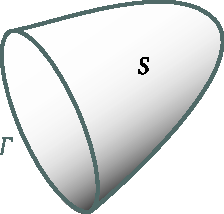
\includegraphics[scale=1]{figures/ch_01/fig_1_32.pdf}
			\caption[]{}
			\label{fig:1_32}
		\end{center}
	\end{minipage}
	\hspace{-0.1cm}
	\begin{minipage}[t]{0.5\linewidth}
		\begin{center}
			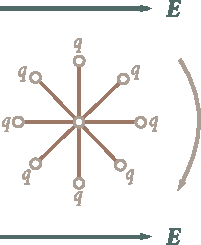
\includegraphics[scale=1]{figures/ch_01/fig_1_33.pdf}
			\caption[]{}
			\label{fig:1_33}
		\end{center}
	\end{minipage}
\vspace{-0.4cm}
\end{figure}

By analogy with the fan impeller shown in \fig{1_25}, let us imagine an electrical ``impeller'' in the form of a light hub with spokes whose ends carry identical positive charges $q$ (\fig{1_33}; the entire arrangement must be small in size). At the points of an electric field where $\curl{\vec{E}}$ differs from zero, such an impeller would rotate with an acceleration that is the greater, the larger is the projection of the curl onto the impeller axis. For an electrostatic field, such an imaginary arrangement would not rotate with any orientation of its axis.

Thus, a feature of an electrostatic field is that it is a non-circuital one. We established in the preceding section that the curl of the gradient of a scalar function equals zero [see expression \eqref{eq:1_96}]. Therefore, the equality to zero of $\curl{\vec{E}}$ at every point of a field makes it possible to represent $\vec{E}$ in the form of the gradient of a scalar function $\varphi$ called the potential. We have already considered this representation in \sect{1_8} [see \eqn{1_41}; the minus sign in this equation was taken from physical considerations].

We can immediately conclude from the need to observe condition \eqref{eq:1_110} that the existence of an electrostatic field of the kind shown in \fig{1_34} is impossible. Indeed, for such a field, the circulation around the contour shown by the dash line would differ from zero, which contradicts condition \eqref{eq:1_110}. It is also impossible for a field differing from zero in a restricted volume to be homogeneous throughout this volume (\fig{1_35}). In this case, the circulation around the contour shown by the dash line would differ from zero.

\begin{figure}[t]
	\begin{minipage}[t]{0.36\linewidth}
		\begin{center}
			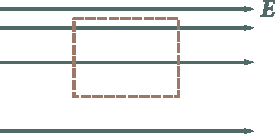
\includegraphics[scale=0.93]{figures/ch_01/fig_1_34.pdf}
			\caption[]{}
			\label{fig:1_34}
		\end{center}
	\end{minipage}
	% \hspace{-0.05cm}
	\hfill{ }
	\begin{minipage}[t]{0.2\linewidth}
		\begin{center}
			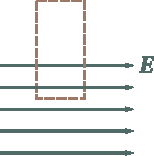
\includegraphics[scale=0.93]{figures/ch_01/fig_1_35.pdf}
			\caption[]{}
			\label{fig:1_35}
		\end{center}
	\end{minipage}
	% \hspace{-0.05cm}
	\hfill{ }
	\begin{minipage}[t]{0.37\linewidth}
		\begin{center}
			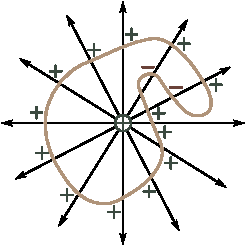
\includegraphics[scale=0.95]{figures/ch_01/fig_1_36.pdf}
			\caption[]{}
			\label{fig:1_36}
		\end{center}
	\end{minipage}
\vspace{-0.5cm}
\end{figure}

\section{Gauss's Theorem}\label{sec:1_13}

We established in the preceding section what the curl of an electrostatic field equals. Now let us find the divergence of a field. For this purpose, we shall consider the field of a point charge $q$ and calculate the flux of the vector $\vec{E}$ through closed surface $S$ surrounding the charge (\fig{1_36}). We showed in \sect{1_5} that the number of lines of the vector $\vec{E}$ beginning at a point charge $+q$ or terminating at a charge $-q$ numerically equals $q/\varepsilon_0$.

By \eqn{1_77}, the flux of the vector $\vec{E}$ through any closed surface equals the number of lines coming out, \ie, beginning on the
charge, if it is positive, and the number of lines entering the surface, \ie, terminating on the charge, if it is negative. Taking into account that the number of lines beginning or terminating at a point charge numerically equals $q/\varepsilon_0$ (see \sect{1_5}), we can write that
\begin{equation}\label{eq:1_113}
	\Phi_E = \frac{q}{\varepsilon_0}.
\end{equation}

\noindent
The sign of the flux coincides with that of the charge $q$. The dimensions of both sides of \eqn{1_113} are identical.

Now let us assume that a closed surface surrounds $N$ point charges $q_1, q_2, \ldots, q_N$. On the basis of the superposition principle, the strength $\vec{E}$ of the field set up by all the charges equals the sum of the strengths $\vec{E}_i$  set up by each charge separately: $\vec{E}=\sum_i\vec{E}_i$. Hence,
\begin{equation*}
	\Phi_E = \oint_S \vec{E}\ccdot\deriv{\vec{S}} = \oint_S \parenthesis{\sum_i\vec{E}_i}\ccdot\deriv{\vec{S}} = \sum_i\oint_S\vec{E}_i\ccdot\deriv{\vec{S}}.
\end{equation*}

\noindent
Each of the integrals inside the sum sign equals $q_i/\varepsilon_0$. Therefore,
\begin{equation}\label{eq:1_114}
	\Phi_E = \oint_S \vec{E}\ccdot\deriv{\vec{S}} = \frac{1}{\varepsilon_0} \sum_{i=1}^N q_i.
\end{equation}

\noindent
The statement we have proved is called \textbf{Gauss's theorem}. According to it, \textit{the flux of an electric field strength vector through a closed surface equals the algebraic sum of the charges enclosed by this surface divided by $\varepsilon_0$}.

When considering fields set up by macroscopic charges (\ie, charges formed by an enormous number of elementary charges), the discrete structure of these charges is disregarded, and they are considered to be distributed in space continuously with a finite density everywhere. The \textbf{volume density of a charge} $\rho$ is determined by analogy with the density of a mass as the ratio of the charge $\deriv{q}$ to the infinitely small (physically) volume $\deriv{V}$ containing this charge:
\begin{equation}\label{eq:1_115}
	\rho = \diff{q}{V}.
\end{equation}

\noindent
In the given case by an infinitely small (physically) volume, we must understand a volume which on the one hand is sufficiently small for the density within its limits to be considered identical, and on the other is sufficiently great for the discreteness of the charge not to manifest itself.

Knowing the charge density at every point of space, we can find the total charge surrounded by closed surface $S$. For this purpose, we must calculate the integral of $\rho$ with respect to the volume enclosed by the surface:
\begin{equation*}
	\sum_i q_i = \int_V \rho\,\deriv{V}.
\end{equation*}

\noindent
Thus, \eqn{1_114} can be written in the form
\begin{equation}\label{eq:1_116}
	\oint_S \vec{E}\ccdot\deriv{\vec{S}} = \frac{1}{\varepsilon_0} \int_V \rho\,\deriv{V}.
\end{equation}

Replacing the surface integral with a volume one in accordance with \eqn{1_108}, we have
\begin{equation*}
	\int_V \divop{\vec{E}}\,\deriv{V} = \frac{1}{\varepsilon_0} \int_V \rho\,\deriv{V}.
\end{equation*}

\noindent
The relation which we have arrived at must be observed for any arbitrarily chosen volume $V$. This is possible only if the values of the integrands for every point of space are the same. Hence, the divergence of the vector $\vec{E}$ is associated with the density of the charge at the same point by the equation
\begin{equation}\label{eq:1_117}
	\divop{\vec{E}} = \frac{1}{\varepsilon_0} \rho.
\end{equation}

\noindent
This equation expresses Gauss's theorem in the differential form.

For a flowing liquid, $\divop{\vec{v}}$ gives the unit power of the sources of the liquid at a given point. By analogy, charges are said to be sources of an electric field.

\section{Calculating Fields with the Aid of Gauss's Theorem}\label{sec:1_14}

Gauss's theorem permits us in a number of cases to find the strength of a field in a much simpler way than by using \eqn{1_15} for the field strength of a point charge and the field superposition principle. We shall demonstrate the possibilities of Gauss's theorem by employing a few examples that will be useful for our further exposition. Before starting on our way, we shall introduce the concepts of surface and linear charge densities.

If a charge is concentrated in a thin surface layer of the body carrying the charge, the distribution of the charge in space can be characterized by the surface density $\sigma$, which is determined by the expression
\begin{equation}\label{eq:1_118}
	\sigma = \diff{q}{S}.
\end{equation}

\noindent
Here $\deriv{q}$ is the charge contained in the layer of area $\deriv{S}$. By $\deriv{S}$ is meant an infinitely small (physically) section of the surface.

If a charge is distributed over the volume or surface of a cylindrical body (uniformly in each section), the linear charge density is used, \ie,
\begin{equation}\label{eq:1_119}
	\lambda = \diff{q}{l}
\end{equation}

\noindent
where $\deriv{l}$ is the length of an infinitely small (physically) segment of the cylinder, and $\deriv{q}$ is the charge concentrated on this segment.

\textbf{Field of an Infinite Homogeneously Charged Plane.} Assume that the surface charge density at all points of a plane is identical and equal to $\sigma$; for definiteness we shall consider the charge to be positive. It follows from considerations of symmetry that the field strength at any point is directed at right angles to the plane. Indeed, since the plane is infinite and charged homogeneously, there is no reason why the vector $\vec{E}$ should deflect to a side from a normal to the plane. It is further evident that at points symmetrical relative to the plane, the field strength is identical in magnitude and opposite in direction.

\begin{figure}[t]
	\begin{minipage}[t]{0.5\linewidth}
		\begin{center}
			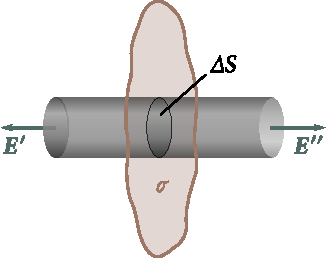
\includegraphics[scale=1]{figures/ch_01/fig_1_37.pdf}
			\caption[]{}
			\label{fig:1_37}
		\end{center}
	\end{minipage}
	\hspace{-0.05cm}
	\begin{minipage}[t]{0.5\linewidth}
		\begin{center}
			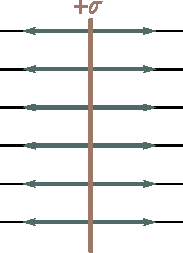
\includegraphics[scale=1]{figures/ch_01/fig_1_38.pdf}
			\caption[]{}
			\label{fig:1_38}
		\end{center}
	\end{minipage}
\vspace{-0.4cm}
\end{figure}

Let us imagine mentally a cylindrical surface with generatrices perpendicular to the plane and bases of a size $\Delta{S}$ arranged symmetrically relative to the plane (\fig{1_37}). Owing to symmetry, we have $E'=E''=E$. We shall apply Gauss's theorem to the surface. The flux through the side part of the surface will be absent because $E_n$ at each point of it is zero. For the bases, $E_n$ coincides with $E$. Hence, the total flux through the surface is $2E\Delta{S}$. The surface encloses the charge $\sigma\Delta{S}$. According to Gauss's theorem, the condition must be observed that
\begin{equation*}
	2E\Delta{S} = \frac{\sigma\Delta{S}}{\varepsilon_0}
\end{equation*}

\noindent
whence
\begin{equation}\label{eq:1_120}
	E = \frac{\sigma}{2\varepsilon_0}.
\end{equation}

\noindent
The result we have obtained does not depend on the length of the cylinder. This signifies that at any distances from the plane, the field strength is identical in magnitude. The field lines are shown in \fig{1_38}. For a negatively charged plane, the result will be the same except for the reversal of the direction of the vector $\vec{E}$ and the field lines.

If we take a plane of finite dimensions, for instance a charged thin plate\footnote{For a plate, by $\sigma$ in \eqn{1_120} should be understood the charge concentrated on \SI{1}{\metre\squared} of the plate over its entire thickness. In metal bodies, the charge is distributed over the external surface. Therefore by $\sigma$ we should understand the double value of the charge density on the surfaces surrounding the metal plate.}, then the result obtained above will hold only for points, the distance to which from the edge of the plate considerably exceeds the distance from the plate itself (in \fig{1_39} the region containing such points is outlined by a dash line). At points at an increasing distance from the plane or approaching its edges, the field will differ more and more from that of an infinitely charged plane. It is easy to imagine the nature of the field at great distances if we take into account that at distances considerably exceeding the dimensions of the plate, the field it sets up can be treated as that of a point charge.

\textbf{Field of Two Uniformly Charged Planes.} The field of two parallel infinite planes carrying opposite charges with a constant surface density $\sigma$ identical in magnitude can be found by superposition of the fields produced by each plane separately (\fig{1_40}). In the region between the planes, the fields being added have the same direction, so that the resultant field strength is
\begin{equation}\label{eq:1_121}
	E = \frac{\sigma}{\varepsilon_0}.
\end{equation}

\noindent
Outside the volume bounded by the planes, the fields being added have opposite directions so that the resultant field strength equals zero.

\begin{figure}[t]
	\begin{minipage}[t]{0.5\linewidth}
		\begin{center}
			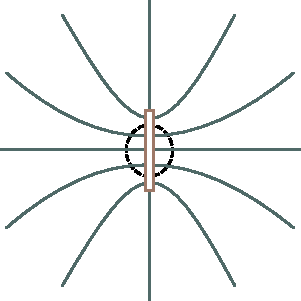
\includegraphics[scale=1]{figures/ch_01/fig_1_39.pdf}
			\caption[]{}
			\label{fig:1_39}
		\end{center}
	\end{minipage}
	\hspace{-0.05cm}
	\begin{minipage}[t]{0.5\linewidth}
		\begin{center}
			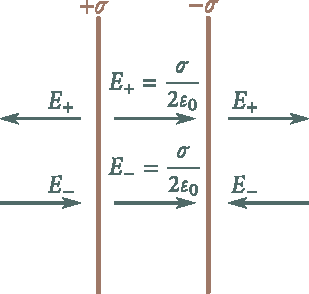
\includegraphics[scale=1]{figures/ch_01/fig_1_40.pdf}
			\caption[]{}
			\label{fig:1_40}
		\end{center}
	\end{minipage}
\vspace{-0.55cm}
\end{figure}

Thus, the field is concentrated between the planes. The field strength at all points of this region is identical in value and in direction; consequently, the field is homogeneous. The field lines are a collection of parallel equispaced straight lines.

The result we have obtained also holds approximately for planes of finite dimensions if the distance between them is much smaller than their linear dimensions (a parallel-plate capacitor). In this case, appreciable deviations of the field from homogeneity are observed only near the edges of the plates (\fig{1_41}).

\textbf{Field of an Infinite Charged Cylinder.} Assume that the field is produced by an infinite cylindrical surface of radius $R$ whose charge has a constant surface density $\sigma$. Considerations of symmetry show that the field strength at any point must be directed along a radial line perpendicular to the cylinder axis, and that the magnitude of the strength can depend only on the distance $r$ from the cylinder axis. Let us mentally imagine a coaxial closed cylindrical surface of radius $r$ and height $h$ with a charged surface (\fig{1_42}). For the bases of the cylinder, we have $E_n=0$, for the side surface $E_n=E(r)$ (the charge is assumed to be positive). Hence, the flux of the vector $\vec{E}$ through the surface being considered is $E(r)\times 2\pi rh$. If $r>R$, the charge $q=\lambda h$ (where $\lambda$ is the linear charge density) will get into the surface. Applying Gauss's theorem, we find that
\begin{equation*}
	E(r)\times 2\pi rh = \frac{2\lambda}{\varepsilon_0}.
\end{equation*}

\noindent
Hence,
\begin{equation}\label{eq:1_122}
	E(r) = \frac{1}{2\pi\varepsilon_0}\frac{\lambda}{r}\quad (r\geqslant R).
\end{equation}

\noindent
If $r<R$, the closed surface being considered contains no charges inside, owing to which $E(r)=0$.

\begin{figure}[t]
	\begin{minipage}[t]{0.35\linewidth}
		\begin{center}
			
\includegraphics[scale=1]{figures/ch_01/fig_1_41.pdf}
			\caption[]{}
			\label{fig:1_41}
		\end{center}
	\end{minipage}
	\hspace{-0.05cm}
	\begin{minipage}[t]{0.65\linewidth}
		\begin{center}
			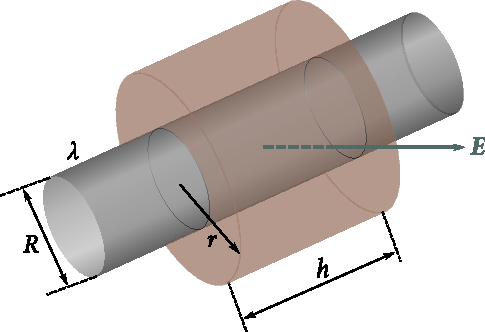
\includegraphics[scale=0.95]{figures/ch_01/fig_1_42.pdf}
			\caption[]{}
			\label{fig:1_42}
		\end{center}
	\end{minipage}
\vspace{-0.4cm}
\end{figure}

Thus, there is no field inside a uniformly charged cylindrical surface of infinite length. The field strength outside the surface is determined by the linear charge density $\lambda$ and the distance $r$ from the cylinder axis.

The field of a negatively charged cylinder differs from that of a positively charged one only in the direction of the vector $\vec{E}$. A glance at \eqn{1_122} shows that by reducing the cylinder radius $R$ (with a constant linear charge density $\lambda$), we can obtain a field with a very great strength near the surface of the cylinder.

Introducing $\lambda=2\pi R\sigma$ into \eqn{1_122} and assuming that $r=R$, we get the following value for the field strength in direct proximity to the surface of a cylinder:
\vspace{-12pt}
\begin{equation}\label{eq:1_123}
	E(R) = \frac{\sigma}{\varepsilon_0}.
\end{equation}

The superposition principle makes it simple to find the field of two coaxial cylindrical surfaces carrying a linear charge density $\lambda$ of the same magnitude, but of opposite signs (\fig{1_43}). There is no field inside the smaller and outside the larger cylinders. The field strength in the gap between the cylinders is determined by \eqn{1_122}. This also holds for cylindrical surfaces of a finite length if the gap between the surfaces is much smaller than their length (a cylindrical capacitor). Appreciable deviations from the field of surfaces of an infinite length will be observed only near the edges of the cylinders.

\begin{figure}[t]
	\begin{center}
		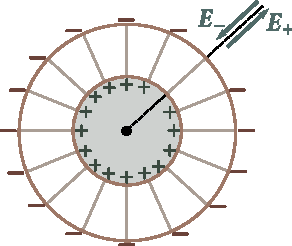
\includegraphics[scale=1]{figures/ch_01/fig_1_43.pdf}
		\caption[]{}
		\label{fig:1_43}
	\end{center}
	\vspace{-0.8cm}
\end{figure}

\textbf{Field of a Charged Spherical Surface.} The field produced by a spherical surface of radius $R$ whose charge has a constant surface density $\sigma$ will obviously be a centrally symmetrical one. This signifies that the direction of the vector $\vec{E}$ at any point passes through the centre of the sphere, while the magnitude of the field strength is a function of the distance $r$ from the centre of the sphere. Let us imagine a surface of radius $r$ that is concentric with the charged sphere. For all points of this surface, $E_n=E(r)$. If $r>R$, the entire charge $q$ distributed over the sphere will be inside the surface. Hence,
\begin{equation*}
	E(r)\times 4\pi r^2 = \frac{q}{\varepsilon_0}
\end{equation*}

\noindent
whence
\begin{equation}\label{eq:1_124}
	E(r) = \frac{1}{4\pi\varepsilon_0}\frac{q}{r^2}.\quad (r\geqslant R)
\end{equation}

A spherical surface of radius $r$ less than $R$ will contain no charges, owing to which for $r<R$ we get $E(r)=0$.

Thus, there is no field inside a spherical surface whose charge has a constant surface density $\sigma$. Outside this surface, the field is identical with that of a point charge of the same magnitude at the
centre of the sphere.

Using the superposition principle, it is easy to show that the field of two concentric spherical surfaces (a spherical capacitor) carrying charges $+q$ and $-q$ that are identical in magnitude and opposite in sign is concentrated in the gap between the surfaces, the magnitude of the field strength in the gap being determined by \eqn{1_124}.

\textbf{Field of a Volume-Charged Sphere.} Assume that a sphere of radius $R$ has a charge with a constant volume density $\rho$. The field in this case has central symmetry. It is easy to see that the same result is obtained for the field outside the sphere [see \eqn{1_124}] as for a sphere with a surface charge. The result will be different for points inside the sphere, however. A spherical surface of radius $r$ ($r<R$) contains a charge equal to $\rho\times 4\pi r^3/3$. Therefore, Gauss's theorem for such a surface will be written as follows:
\begin{equation*}
	E(r)\times 4\pi r^2 = \frac{1}{\varepsilon_0}\rho \frac{4}{3}\pi r^3.
\end{equation*}

\noindent
Hence, substituting $q/(4\pi R^3/3)$ for $\rho$, we get
\begin{equation}\label{eq:1_125}
	E(r) = \frac{1}{4\pi\varepsilon_0}\frac{q}{R^3}r.\quad (r\leqslant R)
\end{equation}

Thus, the field strength inside a sphere grows linearly with the distance $r$ from the centre of the sphere. Outside the sphere, the field strength diminishes according to the same law as for the field of a point charge.

\cleardoublepage
% !TEX root = saveliev_physics_general_course_2.tex
%!TEX TS-program = pdflatex
%!TEX encoding = UTF-8 Unicode


\chapter{ELECTRIC FIELD IN DIELECTRICS}\label{chap:2}

\section{Polar and Non-Polar Molecules}\label{sec:2_1}

Dielectrics (or insulators) are defined as substances not capable of conducting an electric current. Ideal insulators do not exist in nature. All substances, even if to a negligible extent, conduct an electric current. But substances called conductors conduct a current from \num{e15} to \num{e20} times better than substances called dielectrics.

If a dielectric is introduced into an electric field, then the field and the dielectric itself undergo appreciable changes. To understand why this happens, we must take into account that atoms and molecules contain positively charged nuclei and negatively charged electrons.

A molecule is a system with a total charge of zero. The linear dimensions of this system are very small, of the order of a few angstroms (the angstrom---\si{\angstrom}---is a unit of length equal to \SI{e-10}{\metre} that is very convenient in atomic physics). We established in \sect{1_10} that the field set up by such a system is determined by the magnitude and orientation of the dipole electric moment
\begin{equation}\label{eq:2_1}
    \vec{p} = \sum_i q_i \vec{r}_i
\end{equation}

\noindent
(summation is performed both over the electrons and over the nuclei). True, the electrons in a molecule are in motion, so that this moment constantly changes. The velocities of the electrons are so high, however, that the mean value of the moment \eqref{eq:2_1} is detected in practice. For this reason in the following by the dipole moment of a molecule, we shall mean the quantity
\begin{equation}\label{eq:2_2}
    \vec{p} = \sum_i q_i \average{\vec{r}_i}
\end{equation}

\noindent
(for nuclei, $\vec{r}_i$ is simply taken as $\average{\vec{r}_i}$ in this sum). In other words, we shall consider that the electrons are at rest relative to the nuclei at certain points obtained by averaging the positions of the electrons in time.

The behaviour of a molecule in an external electric field is also determined by its dipole moment. We can verify this by calculating the potential energy of a molecule in an external electric field. Selecting the origin of coordinates inside the molecule and taking advantage of the smallness of $\average{\vec{r}_i}$, let us write the potential at the point where the $i$-th charge is in the form
\begin{equation*}
    \varphi_i = \varphi + \gradop{\varphi} \ccdot \average{\vec{r}_i}
\end{equation*}

\noindent
where $\varphi$ is the potential at the origin of coordinates [see \eqn{1_69}]. Hence,
\begin{equation*}
    \ab{W}{p} = \sum_i q_i \varphi_i = \sum_i q_i \parenthesis{\varphi + \gradop{\varphi} \ccdot \average{\vec{r}_i}} = \varphi \sum_i q_i + \gradop{\varphi} \sum_i q_i \average{\vec{r}_i}.
\end{equation*}

\noindent
Taking into account that $\sum_i q_i=0$ and substituting $-\vec{E}$ for $\gradop{\varphi}$, we get
\begin{equation*}
    \ab{W}{p} = -\vec{E} \sum_i q_i \average{\vec{r}_i} = -\vecdot{p}{E} = -p E \cos\alpha.
\end{equation*}

\noindent
Differentiating this expression with respect to $\alpha$, we get \eqn{1_57} for the rotational moment; differentiating with respect to $x$, we arrive at the force \eqref{eq:1_62}.

Thus, a molecule is equivalent to a dipole both with respect to the field it sets up and with respect to the forces it experiences in an external field. The positive charge of this dipole equals the total charge of the nuclei and is at the ``centre of gravity'' of the positive charges; the negative charge equals the total charge of the electrons and is at the ``centre of gravity'' of the negative charges.

In symmetrical molecules (such as \ce{H2},\ce{O2}, \ce{N2}), the centres of gravity of the positive and negative charges coincide in the absence of an external electric field. Such molecules have no intrinsic dipole moment and are called \textbf{non-polar}. In asymmetrical molecules (such
as \ce{CO}, \ce{NH}, \ce{HCl}), the centres of gravity of the charges of opposite signs are displaced relative to each other. In this case, the molecules have an intrinsic dipole moment and are called \textbf{polar}.

Under the action of an external electric field, the charges in a non-polar molecule become displaced relative to one another, the positive ones in the direction of the field, the negative ones against the field. As a result, the molecule acquires a dipole moment whose magnitude, as shown by experiments, is proportional to the field strength (intensity). In the rationalized system, the constant of proportionality is written in the form $\varepsilon_0\beta$, where $\varepsilon_0$ is the electric constant, and $\beta$ is a quantity called the \textbf{polarizability of a molecule}. Since the directions of $\vec{p}$ and $\vec{E}$ coincide, we can write that
\begin{equation}\label{eq:2_3}
    \vec{p} = \beta \varepsilon_0 \vec{E}.
\end{equation}

\noindent
The dipole moment has a dimension of [$q$]L. By \eqn{1_15}, the dimension of $\varepsilon_0\vec{E}$ is [$q$]L$^{-2}$. Hence, the polarizability of a molecule $\beta$ has the dimension L$^3$.

The process of polarization of a non-polar molecule proceeds as if the positive and negative charges of the molecule were bound to one another by elastic forces. A non-polar molecule is, therefore said, to behave in an external field like an elastic dipole.

The action of an external field on a polar molecule consists mainly in tending to rotate the molecule so that its dipole moment is arranged in the direction of the field. An external field does not virtually affect the magnitude of a dipole moment. Consequently, a polar molecule behaves in an external field like a rigid dipole.

\section{Polarization of Dielectrics}\label{sec:2_2}

In the absence of an external electric field, the dipole moments of the molecules of a dielectric usually either equal zero (non-polar molecules) or are distributed in space by directions chaotically (polar molecules). In both cases, the total dipole moment of a dielectric equals zero\footnote{In \sect{2_9}, we shall acquaint ourselves with substances that can have a dipole moment in the absence of an external field.}.

A dielectric becomes polarized under the action of an external field. This signifies that the resultant dipole moment of the dielectric becomes other than zero. It is quite natural to take the dipole moment of a unit volume as the quantity characterizing the degree of polarization. If the field or the dielectric (or both) are not homogeneous, the degrees of polarization at different points of the dielectric will differ. To characterize the polarization at a given point, we must separate an infinitely small (physically) volume $\Delta{V}$ containing this point, find the sum $\sum_{\Delta{V}}\vec{p}$ of the moments of the molecules confined in this volume, and take the ratio
\begin{equation}\label{eq:2_4}
    \vec{P} = \frac{\displaystyle\sum_{\Delta{V}}\vec{p}}{\Delta{V}}.
\end{equation}

\noindent
The vector quantity $\vec{P}$ defined by \eqn{2_4} is called the \textbf{polarization of a dielectric}.

The dipole moment $\vec{p}$ has the dimension [$q$]L. Consequently, the dimension of $\vec{P}$ is [$q$]L$^{-2}$, \ie, it coincides with the dimension of $\varepsilon_0\vec{E}$ [see \eqn{1_15}].

The polarization of isotropic dielectrics of any kind is associated with the field strength at the same point by the simple relation
\begin{equation}\label{eq:2_5}
    \vec{P} = \chi \varepsilon_0 \vec{E}
\end{equation}

\noindent
where $\chi$ is a quantity independent of $\vec{E}$ called the \textbf{electric susceptibility of a dielectric}\footnote{In anisotropic dielectrics, the directions of $\vec{P}$ and $\vec{E}$, generally speaking,
do not coincide. In this case, the relation between $\vec{P}$ and $\vec{E}$ is described by the equations
\begin{align*}
    P_x &= \varepsilon\parenthesis{\chi_{xx}E_x + \chi_{xy}E_y+\chi_{xz}E_z},\\
    P_y &= \varepsilon\parenthesis{\chi_{yx}E_x + \chi_{yy}E_y+\chi_{yz}E_z},\\
    P_z &= \varepsilon\parenthesis{\chi_{zx}E_x + \chi_{zy}E_y+\chi_{zz}E_z}.
\end{align*}

\noindent
The combination of the nine quantities $\chi_{ij}$ forms a symmetrical tensor of rank two called the \textbf{tensor of the dielectric susceptibility} [compare with Eqs. (5.30)
of Vol. I). This tensor characterizes the electrical properties of an anisotropic dielectric.}. It was indicated above that the dimensions of $\vec{P}$ and $\varepsilon_0\vec{E}$ are identical. Hence, $\chi$ is a dimensionless quantity.

In the Gaussian system of units, \eqn{2_5} has the form
\begin{equation}\label{eq:2_6}
    \vec{P} = \chi \vec{E}.
\end{equation}

For dielectrics built of non-polar molecules, \eqn{2_5} issues from the following simple considerations. The volume $\Delta{V}$ contains a number of molecules equal to $n\Delta{V}$, where $n$ is the number of molecules per unit volume. Each of the moments $\vec{p}$ is determined in this case by \eqn{2_3}. Hence,
\begin{equation*}
    \sum{\Delta{V}} \vec{p} = n \Delta{V} \beta \varepsilon_0 \vec{E}.
\end{equation*}

\noindent
Dividing this expression by $\Delta{V}$, we get the polarization $\vec{P}=n\beta\varepsilon_0\vec{E}$. Finally, introducing the symbol $\chi=n\beta$, we arrive at \eqn{2_5}.

For dielectrics built of polar molecules, the orienting action of the external field is counteracted by the thermal motion of the molecules tending to scatter their dipole moments in all directions. As a result, a certain preferred orientation of the dipole moments of the molecules sets in in the direction of the field. The relevant statistical calculations, which agree with experimental data, show that the polarization is proportional to the field strength, \ie, leads to \eqn{2_5}. The electric susceptibility of such dielectrics varies inversely with the absolute temperature.

In ionic crystals, the separate molecules lose their individuality. An entire crystal is, as it were, a single giant molecule. The lattice of an ionic crystal can be considered as two lattices inserted into each other, one of which is formed by the positive, and the other by the negative ions. When an external field acts on the crystal ions, both lattices are displaced relative to each other, which leads to polarization of the dielectric. The polarization in this case too is associated with the field strength by \eqn{2_5}. We must note that the linear relation between $\vec{E}$ and $\vec{P}$ described by \eqn{2_5} may be applied only to not too strong fields [a similar remark relates to \eqn{2_3}].

\section{The Field Inside a Dielectric}\label{sec:2_3}

The charges in the molecules of a dielectric are called \textbf{bound}. The action of a field can only cause bound charges to be displaced slightly from their equilibrium positions; they cannot leave the molecule containing them.

Following the example of L. Landau and E. Lifshitz\footnote{See L. D. Landau and E. M. Lifshitz. Elektrodinamika sploshnykh sred (Electrodynamics of Continuous Media). Moscow, Gostekhizdat (1957), p. 57.}, we shall call charges that, although they are within the boundaries of a dielectric, are not inside its molecules, and also charges outside a dielectric, extraneous ones\footnote{It is customary practice to call such charges \textbf{free}. This name is extremely unsuccessful, however, because in a number of cases extraneous charges are not at all free.}.

The field in a dielectric is the superposition of the field $\ab{\vec{E}}{extr}$ produced by the extraneous charges, and the field $\ab{\vec{E}}{bound}$ of the bound charges. The resultant field is called \textbf{microscopic} (or \textbf{true}):
\begin{equation}\label{eq:2_7}
    \ab{\vec{E}}{micro} = \ab{\vec{E}}{extr} + \ab{\vec{E}}{bound}.
\end{equation}

The microscopic field changes greatly within the limits of the intermolecular distances. Owing to the motion of the bound charges, the field $\ab{\vec{E}}{micro}$ also changes with time. These changes are not detected in a macroscopic-consideration. Therefore, a field is characterized by the quantity \eqref{eq:2_7} averaged over an infinitely small (physically) volume, \ie,
\begin{equation*}
    \vec{E} = \average{\ab{\vec{E}}{micro}} = \average{\ab{\vec{E}}{extr}} + \average{\ab{\vec{E}}{bound}}.
\end{equation*}

In the following, we shall designate the averaged field of the extraneous charges by $\vec{E}_0$, and the averaged field of the bound charges by $\vec{E}'$. Accordingly, we shall define a macroscopic field as the quantity
\begin{equation}\label{eq:2_8}
    \vec{E} = \vec{E}_0 + \vec{E}'.
\end{equation}

The polarization $\vec{P}$ is a macroscopic quantity. Therefore, $\vec{E}$ in \eqn{2_5} should be understood as the strength determined by \eqn{2_8}.

In the absence of dielectrics (\ie, in a ``vacuum''), the macroscopic field is
\begin{equation*}
    \vec{E} = \vec{E}_0 = \average{\ab{\vec{E}}{extr}}.
\end{equation*}

\noindent
It is exactly this quantity that is understood to be $\vec{E}$ in \eqn{1_117}.

If the extraneous charges are stationary, the field determined by \eqn{2_8} has the same properties as an electrostatic field in a vacuum. In particular, it can be characterized with the aid of the potential $\varphi$ related to the field strength \eqref{eq:2_8} by Eqs. \eqref{eq:1_41} and \eqref{eq:1_45}.

\section{Space and Surface Bound Charges}\label{sec:2_4}

When a dielectric is not polarized, the volume density $\rho'$ and the surface density $\sigma'$ of the bound charges equal zero. Polarization causes the surface density, and in some cases also the volume density of the bound charges to become different from zero.

Figure \ref{fig:2_1} shows schematically a polarized dielectric with nonpolar (a) and polar (b) molecules. Inspection of the figure shows that the polarization is attended by the appearance of a surplus of bound charges of one sign in the thin surface layer of the dielectric. If the normal component of the field strength $\vec{E}$ for the given section of the surface is other than zero, then under the action of the field, charges of one sign will move away inward, and of the other sign will emerge.

\begin{figure}[t]
	\begin{minipage}[t]{0.64\linewidth}
		\begin{center}
			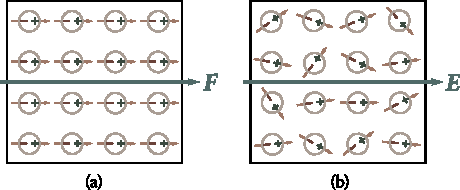
\includegraphics[scale=1]{figures/ch_02/fig_2_1.pdf}
			\caption[]{}
			\label{fig:2_1}
		\end{center}
	\end{minipage}
	\hfill{}%space{-0.05cm}
	\begin{minipage}[t]{0.34\linewidth}
		\begin{center}
			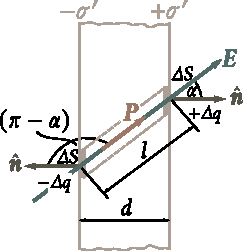
\includegraphics[scale=1]{figures/ch_02/fig_2_2.pdf}
			\caption[]{}
			\label{fig:2_2}
		\end{center}
	\end{minipage}
\vspace{-0.4cm}
\end{figure}

There is a simple relation between the polarization $\vec{P}$ and the surface density of the bound charges $\sigma'$. To find it, let us consider an infinite plane-parallel plate of a homogeneous dielectric placed in a homogeneous electric field (\fig{2_2}). Let us mentally separate an elementary volume in the plate in the form of a very thin cylinder with generatrices parallel to $\vec{E}$ in the dielectric, and with bases of area $\Delta{S}$ coinciding with the surfaces of the plate. The magnitude of this volume is
\begin{equation*}
    \Delta{V} = l \Delta{S} \cos\alpha
\end{equation*}

\noindent
where $l$ is the distance between the bases of the cylinder and $\alpha$ the angle between the vector $\vec{E}$ and an outward normal to the positively charged surface of the dielectric.

The volume $\Delta{V}$ has a dipole electric moment of the magnitude
\begin{equation*}
    P\Delta{V} = Pl\Delta{S}\cos\alpha
\end{equation*}

\noindent
($P$ is the magnitude of the polarization).

From the macroscopic viewpoint, the volume being considered is equivalent to a dipole formed by the $+\sigma'\Delta{S}$ and $-\sigma'\Delta{S}$ with a spacing of $l$. Therefore, its electric moment can be written in the form $\sigma'\Delta{S}l$. Equating the two expressions for the electric moment, we get
\begin{equation*}
    Pl\Delta{S}\cos\alpha = \sigma'\Delta{S}l.
\end{equation*}

\noindent
Hence, we get the required relation between $\sigma'$ and $\vec{P}$:
\begin{equation}\label{eq:2_9}
    \sigma' = P \cos\alpha = \ab{P}{n}
\end{equation}

\noindent
where $\ab{P}{n}$ is the projection of the polarization onto an outward normal to the relevant surface. For the right-hand surface in \fig{2_2}, we have $\ab{P}{n}>0$, accordingly, $\sigma'$ for it is positive; for the left-hand surface $\ab{P}{n}<0$, accordingly, $\sigma'$ for it is negative.

Expressing $\vec{P}$ through $\chi$ and $\vec{E}$ by means of \eqn{2_5}, we arrive at the formula
\begin{equation}\label{eq:2_10}
    \sigma' = \chi \varepsilon_0 \ab{E}{n}
\end{equation}

\noindent
where $\ab{E}{n}$ is the normal component of the field strength inside the dielectric. According to \eqn{2_10}, at the places where the field lines emerge from the dielectric ($\ab{E}{n}>0$), positive bound charges come up to the surface, while where the field lines enter the dielectric ($\ab{E}{n}<0$), negative surface charges appear.

Equations \eqref{eq:2_9} and \eqref{eq:2_10} also hold in the most general case when an inhomogeneous dielectric of an arbitrary shape is in an inhomogeneous electric field. By $\ab{P}{n}$ and $\ab{E}{n}$ in this case, we must understand the normal component of the relevant vector taken in direct proximity to the surface element for which $\sigma'$ is being determined.

Now let us turn to finding the volume density of the bound charges appearing inside an inhomogeneous dielectric. Let us consider an imaginary small area $\Delta{S}$ (\fig{2_3}) in an inhomogeneous isotropic dielectric with non-polar molecules.
Assume that a unit volume of the dielectric has $n$ identical particles with a charge of $+e$ and $n$ identical particles with a charge of $-e$. In close proximity to area $\Delta{S}$, the electric field and the dielectric can be considered homogeneous.
Therefore, when the field is switched on, all the positive charges near $\Delta{S}$ will be displaced over the same distance $l_1$ in the direction of $\vec{E}$, and all the negative charges will be displaced in the opposite direction over the same distance $l_2$ (see \fig{2_3}).
A certain number of charges of one sign (positive if $\alpha<n/2$ and negative if $\alpha>n/2$) will pass through area $\Delta{S}$ in the direction of a normal to it, and a certain number of charges of the opposite sign (negative if $\alpha<n/2$ and positive if $\alpha<n/2$) in the direction opposite to $\hatvec{n}$.
Area $\Delta{S}$ will be intersected by all the charges $+e$ that were at a distance of not over $l_1\cos\alpha$ from it before the field was switched on, \ie, by all the $+e$'s in an oblique cylinder of volume $l_1\Delta{S}\cos\alpha$. The number of these charges is $nl_1\Delta{S}\cos\alpha$, while the charge they carry in the direction of a normal to the area is $enl_1\Delta{S}\cos\alpha$ (when $\alpha>\pi/2$, the charge carried in the direction of the normal as a result of displacement of the charges $+e$ will be negative).
Similarly, area $\Delta{S}$ will be intersected by all the charges $-e$ in the volume $l_2\Delta{S}\cos\alpha$. These charges will carry a charge of $enl_2\Delta{S}\cos\alpha$ in the direction of a normal to the area (inspection of \fig{2_3} shows that when $\alpha<\pi/2$, the charges $-e$ will carry the charge $-enl_2\Delta{S}\cos\alpha$ through $\Delta{S}$ in the direction opposite to $\hatvec{n}$, which is equivalent to carrying the charge $enl_2\Delta{S}\cos\alpha$ in the direction of $\hatvec{n}$).

\begin{figure}[t]
	\begin{center}
		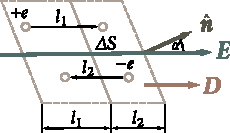
\includegraphics[scale=1.1]{figures/ch_02/fig_2_3.pdf}
		\caption[]{}
		\label{fig:2_3}
	\end{center}
	\vspace{-0.8cm}
\end{figure}

Thus, when the field is switched on, the charge
\begin{equation*}
    \Delta{q}' = enl_1\Delta{S}\cos\alpha + enl_2\Delta{S}\cos\alpha = en (l_1+l_2) \Delta{S} \cos\alpha
\end{equation*}

\noindent
is carried through area $\Delta{S}$ in the direction of a normal to it. The sum $l_1+l_2$ is the distance $l$ over which the positive and negative bound charges are  displaced toward one another in the dielectric. As a result of this displacement, each pair of charges acquires the dipole moment $p=el=e(l_1+l_2)$. The number of such pairs in a unit volume is $n$. Consequently, the product $e(l_1+l_2)n=eln=p$ gives the magnitude of the polarization $P$. Thus, the charge passing through area $\Delta{S}$ in the direction of a normal to it when the field is switched on is [see \eqn{2_9}]
\begin{equation*}
    \Delta{q}' = P \Delta{S} \cos\alpha.
\end{equation*}

Since the dielectric is isotropic, the directions of the vectors $\vec{E}$ and $\vec{P}$ coincide (see \fig{2_3}). Consequently, $\alpha$ is the angle between the vectors $\vec{P}$ and $\hatvec{n}$, and in this connection we can write
\begin{equation*}
    \Delta{q}' = (\vec{P} \ccdot \hatvec{n})\, \Delta{S}.
\end{equation*}

\noindent
Passing over from deltas to differentials, we get
\begin{equation*}
    \deriv{q} = (\vec{P} \ccdot \hatvec{n})\, \deriv{S} = \vec{P} \ccdot \deriv{\vec{S}}.
\end{equation*}

We have found the bound charge $\deriv{q'}$ that passes through elementary area $\deriv{S}$ in the direction of a normal to it when the field is switched on; $\vec{P}$ is the polarization set up under the action of the field at the location of area $\deriv{S}$.

Let us imagine closed surface $S$ inside the dielectric. When the field is switched on, a bound charge $q'$ will intersect this surface and emerge from it. This charge is
\begin{equation*}
    \ab{q'}{em} = \oint_S \deriv{q'} = \oint_S \vec{P} \ccdot \deriv{\vec{S}}
\end{equation*}

\noindent
(we have agreed to take the outward normal to area $\deriv{S}$ for closed surfaces). As a result, a surplus bound charge will appear in the volume enclosed by surface $S$. Its value is
\begin{equation}\label{eq:2_11}
    \ab{q'}{sur} = - \ab{q'}{em} = - \oint_S \vec{P} \ccdot \deriv{\vec{S}} = - \ab{\Phi}{P}
\end{equation}

\noindent
($\ab{\Phi}{P}$ is the flux of the vector $\vec{P}$ through surface $S$).

Introducing the volume density of the bound charges $\rho'$, we can write
\begin{equation*}
    \ab{q'}{sur} = \int_V \rho'\, \deriv{V}
\end{equation*}

\noindent
(the integral is taken over the volume enclosed by surface $S$). We thus arrive at the formula
\begin{equation*}
    \int_V \rho'\, \deriv{V} = - \oint_S \vec{P} \ccdot \deriv{\vec{S}}.
\end{equation*}

\noindent
Let us transform the surface integral according to the Ostrogradsky-Gauss theorem [see \eqn{1_108}). The result is
\begin{equation*}
    \int_V \rho'\, \deriv{V} = - \int_V \divop{\vec{P}}\, \deriv{V}.
\end{equation*}

\noindent
This equation must be observed for any arbitrarily chosen volume $V$. This is possible only if the following equation is observed at every point of the dielectric:
\begin{equation}\label{eq:2_12}
    \rho' = - \divop{\vec{P}}.
\end{equation}

\noindent
Consequently, the density of bound charges equals the divergence of the polarization $\vec{P}$ taken with the opposite sign.

We obtained \eqn{2_12} when considering a dielectric with non-polar molecules. This equation also holds, however, for dielectrics with polar molecules.

\begin{figure}[t]
	\begin{center}
		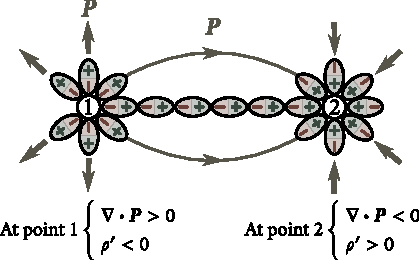
\includegraphics[scale=1]{figures/ch_02/fig_2_4.pdf}
		\caption[]{}
		\label{fig:2_4}
	\end{center}
	\vspace{-0.8cm}
\end{figure}

Equation \eqref{eq:2_12} can be given a graphical interpretation. Points with a positive $\divop{\vec{P}}$ are sources of the field of the vector $\vec{P}$, and the lines of $\vec{P}$ diverge from them (\fig{2_4}). Points with a negative $\divop{\vec{P}}$ are sinks of the field of the vector $\vec{P}$, and the lines of $\vec{P}$ converge at them.
In polarization of the dielectric, the positive bound charges are displaced in the direction of the vector $\vec{P}$, \ie, in the direction of the lines $\vec{P}$; the negative bound charges are displaced in the opposite direction (in the figure the bound charges belonging to separate molecules are encircled by ovals). As a result, a surplus of negative bound charges is formed at places with a positive $\divop{\vec{P}}$, and a surplus of positive bound charges at places with a negative $\divop{\vec{P}}$.

Bound charges differ from extraneous ones only in that they cannot leave the confines of the molecules which they are in. Otherwise, they have the same properties as all other charges. In particular, they are sources of an electric field. Therefore, when the density of the bound charges $\rho'$ differs from zero, \eqn{1_117} must be written in the form
\begin{equation}\label{eq:2_13}
    \divop{\vec{E}} = \frac{1}{\varepsilon_0} \parenthesis{\rho + \rho'}.
\end{equation}

\noindent
Here $\rho$ is the density of the extraneous charges.

Let us introduce \eqn{2_5} for $\vec{P}$ into \eqn{2_12} and use \eqn{1_103}. The result is
\begin{equation*}
    \rho' = - \divop{(\chi\varepsilon_0\vec{E})} = - \varepsilon_0 \divop{(\chi\vec{E})} = - \varepsilon_0 [\vec{E}\ccdot\gradop{\chi} + \chi \divop{\vec{E}}].
\end{equation*}

\noindent
Substituting for $\divop{\vec{E}}$ its value from \eqn{2_13}, we arrive at the equation
\begin{equation*}
    \rho' = - \varepsilon_0 (\vec{E}\ccdot\gradop{\chi}) - \chi\rho - \chi\rho'.
\end{equation*}

\noindent
Hence,
\begin{equation}\label{eq:2_14}
    \rho' = - \parenthesis{\frac{1}{1+\chi}} [\varepsilon_0 (\vec{E}\ccdot\gradop{\chi}) + \chi\rho].
\end{equation}

We can see from \eqn{2_14} that the volume density of bound charges can differ from zero in two cases: (1) if a dielectric is not homogeneous ($\gradop{\chi}\neq 0$), and (2) if at a given place in a dielectric the density of the extraneous charges is other than zero ($\rho\neq 0$).

When there are no extraneous charges in a dielectric, the volume density of the bound charges is
\begin{equation}\label{eq:2_15}
    \rho' = - \parenthesis{\frac{\varepsilon_0}{1+\chi}} (\vec{E}\ccdot\gradop{\chi}).
\end{equation}

\section{Electric Displacement Vector}\label{sec:2_5}

We noted in the preceding section that not only extraneous, but also bound charges are sources of a field. Accordingly,
\begin{equation}\label{eq:2_16}
    \divop{\vec{E}} = \frac{1}{\varepsilon_0} \parenthesis{\rho + \rho'}
\end{equation}

\noindent
[see \eqn{2_13}].

Equation \eqref{eq:2_16} is of virtually no use for finding the vector $\vec{E}$ because it expresses the properties of the unknown quantity $\vec{E}$ through bound charges, which in turn are determined by the unknown quantity $\vec{E}$ [see Eqs. \eqref{eq:2_10} and \eqref{eq:2_14}].

Calculation of the fields is often simplified if we introduce an auxiliary quantity whose sources are only extraneous charges $\rho$. To establish what this quantity looks like, let us introduce \eqn{2_12} for $\rho'$ into \eqn{2_16}:
\begin{equation*}
    \divop{\vec{E}} = \frac{1}{\varepsilon_0} (\rho - \divop{\vec{P}})
\end{equation*}

\noindent
whence it follows that
\begin{equation}\label{eq:2_17}
    \divop{(\varepsilon_0\vec{E} + \vec{P})} = \rho
\end{equation}

\noindent
(we have put $\varepsilon_0$ inside the del symbol). The expression in parentheses in \eqn{2_17} is the required quantity. It is designated by the symbol $\vec{D}$ and is called the electric displacement (or electric induction).

Thus, the \textbf{electric displacement} is a quantity determined by the relation
\begin{equation}\label{eq:2_18}
    \vec{D} = \varepsilon_0\vec{E} + \vec{P}.
\end{equation}

\noindent
Inserting \eqn{2_5} for $\vec{P}$, we get
\begin{equation}\label{eq:2_19}
    \vec{D} = \varepsilon_0\vec{E} + \chi\varepsilon_0\vec{E} = \varepsilon_0 (1+\chi) \vec{E}.
\end{equation}

The dimensionless quantity
\begin{equation}\label{eq:2_20}
    \varepsilon = 1 + \chi
\end{equation}

\noindent
is called the \textbf{relative permittivity} or simply the \textbf{permittivity} of a medium\footnote{The so-called absolute permittivity of a medium $\ab{\varepsilon}{a}=\varepsilon_0\varepsilon$ is introduced in electrical engineering. This quantity is deprived of a physical meaning, however, and we shall not use it.}. Thus, \eqn{2_19} can be written in the form
\begin{equation}\label{eq:2_21}
    \vec{D} = \varepsilon_0 \varepsilon \vec{E}.
\end{equation}

\noindent
According to \eqn{2_21}, the vector $\vec{D}$ is proportional to the vector $\vec{E}$. We remind our reader that we are dealing with isotropic dielectrics. In anisotropic dielectrics, the vectors $\vec{E}$ and $\vec{D}$, generally speaking, are not collinear.

In accordance with Eqs. \eqn{1_15} and \eqn{2_21}, the electric displacement of the field of a point charge in a vacuum is
\begin{equation}\label{eq:2_22}
    \vec{D} = \frac{1}{4\pi} \frac{q}{r^2} \vecuni{r}.
\end{equation}

The unit of electric displacement is the coulomb per square
metre (\si{\coulomb\per\metre\squared}).

Equation \eqref{eq:2_17} can be written as
\begin{equation}\label{eq:2_23}
    \divop{\vec{D}} = \rho.
\end{equation}

\noindent
Integration of this equation over the arbitrary volume $V$ yields
\begin{equation*}
    \int_V \divop{\vec{D}}\, \deriv{V} = \int_V \rho\, \deriv{V}.
\end{equation*}

\noindent
Let us transform the left-hand side according to the Ostrogradsky-Gauss theorem [see \eqn{1_108}]:
\begin{equation}\label{eq:2_24}
    \oint_S \vec{D} \ccdot \deriv{\vec{S}} = \int_V \rho\, \deriv{V}.
\end{equation}

\noindent
The quantity on the left-hand side is $\Phi_D$---the flux of the vector $\vec{D}$ through closed surface $S$, while that on the right-hand side is the sum of the extraneous charges $\sum_iq_i$ enclosed by this surface. Hence, \eqn{2_24} can be written in the form
\begin{equation}\label{eq:2_25}
    \Phi_D = \sum_i q_i.
\end{equation}

\noindent
Equations \eqref{eq:2_24} and \eqref{eq:2_25} express Gauss's theorem for the vector $\vec{D}$: \textit{the flux of the electric displacement through a closed surface equals the algebraic sum of the extraneous charges enclosed by this surface}.

In a vacuum, $\vec{P}=0$, so that the quantity $\vec{D}$ determined by \eqn{2_18} transforms into $\varepsilon_0\vec{E}$, and Eqs. \eqref{eq:2_24} and \eqref{eq:2_25} transform into Eqs. \eqref{eq:1_114} and \eqref{eq:1_116}.

The unit of the flux of the electric displacement vector is the coulomb. By \eqn{2_25}, a charge of \SI{1}{\coulomb} sets up a displacement flux of \SI{1}{\coulomb} through the surface surrounding it.

The field of the vector $\vec{D}$ can be depicted with the aid of electric displacement lines (we shall call them displacement lines for brevity's sake). Their direction and density are determined in exactly the same way as for the lines of the vector $\vec{E}$ (see \sect{1_5}). The lines of the vector $\vec{E}$ can begin and terminate at both extraneous and bound charges. The sources of the field of the vector $\vec{D}$ are only extraneous charges. Hence, displacement lines can begin or terminate only at extraneous charges. These lines pass without interruption through points at which bound charges are placed.

The electric induction\footnote{The term ``electric displacement'' is not applied to quantity \eqref{eq:2_27}.} in the Gaussian system is determined by the expression
\begin{equation}\label{eq:2_26}
    \vec{D} = \vec{E} + 4\pi\vec{P}.
\end{equation}

\noindent
Substituting for $\vec{P}$ in this equation its value from \eqn{2_6}, we get
\begin{equation}\label{eq:2_27}
    \vec{D} = (1 + 4\pi\chi) \vec{E}.
\end{equation}

The quantity
\begin{equation}\label{eq:2_28}
    \varepsilon = 1 + 4\pi\chi.
\end{equation}

\noindent
is called the \textbf{permittivity}. Introducing this quantity into \eqn{2_27} we get
\begin{equation}\label{eq:2_29}
    \vec{D} = \varepsilon \vec{E}.
\end{equation}

In the Gaussian system, the electric induction in a vacuum coincides with the field strength $\vec{E}$. Consequently, the electric induction of the field of a point charge in a vacuum is determined by \eqn{1_16}.

By \eqn{2_22} the electric displacement set up by a charge of \SI{1}{\coulomb} at a distance of \SI{1}{\metre} is
\begin{equation*}
    D = \frac{1}{4\pi}\frac{q}{r^2} = \frac{1}{4\pi\times 1^2} = \frac{1}{4\pi} \si{\coulomb\per\metre\squared}.
\end{equation*}

\noindent
In the Gaussian system, the electric induction in this case is
\begin{equation*}
    D = \frac{q}{r^2} = \frac{\num{3e9}}{\num{e4}} = \SI{3e5}{\cgse{D}}.
\end{equation*}

\noindent
Thus,
\begin{equation*}
    \SI{1}{\coulomb\per\metre\squared} = 4\pi \times  \SI{3e5}{\cgse{D}}.
\end{equation*}

In the Gaussian system, the expressions of Gauss's theorem
have the form
\begin{align}
    \oint_S \vec{D} \ccdot \deriv{\vec{S}} &= 4\pi \int_V \rho\, \deriv{V}\label{eq:2_30}\\
    \Phi_D &= 4\pi \sum_i q_i.\label{eq:2_31}
\end{align}

\noindent
According to \eqn{2_31}, a charge of \SI{1}{\coulomb} sets up a flux of the electric induction vector of $4\pi q=4\pi\times\SI{3e9}{\cgse{\Phi_D}}$. The following relation thus exists between the units of flux of the vector $\vec{D}$:
\begin{equation*}
    \SI{1}{\coulomb} = 4\pi \times \SI{3e9}{\cgse{\Phi_D}}.
\end{equation*}

\section{Examples of Calculating the Field in Dielectrics}\label{sec:2_6}

We shall consider several examples of fields in dielectrics to reveal the meaning of the quantities $\vec{D}$ and $\varepsilon$.

\textbf{Field Inside a Flat Plate.} Let us consider two infinite parallel oppositely charged planes. Let the field they produce in a vacuum be characterized by the strength $\vec{E}_0$ and the displacement $\vec{D}_0=\varepsilon_0\vec{E}_0$. Let us introduce into this field a plate of a homogeneous isotropic dielectric and arrange it as shown in \fig{2_5}. The dielectric becomes polarized under the action of the field, and bound charges of density $\sigma'$ will appear on its surfaces. These charges will set up a homogeneous field inside the plate whose strength by \eqn{1_121} is $E'=\sigma'/\varepsilon_0$. In the given case, $E'=0$ outside the dielectric.

\begin{figure}[t]
	\begin{center}
		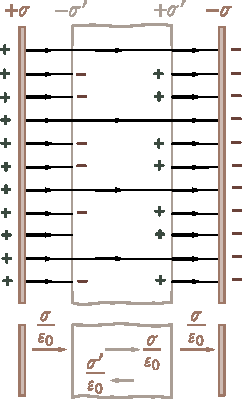
\includegraphics[scale=1]{figures/ch_02/fig_2_5.pdf}
		\caption[]{}
		\label{fig:2_5}
	\end{center}
	\vspace{-0.8cm}
\end{figure}

The field strength $E_0$ is $\sigma/\varepsilon_0$. Both fields are directed toward each other, hence, inside the dielectric we have
\begin{equation}\label{eq:2_32}
    E = E_0 - E' = E_0 - \frac{\sigma'}{\varepsilon_0} = \frac{1}{\varepsilon_0}\parenthesis(\sigma - \sigma').
\end{equation}

\noindent
Outside the dielectric, $E=E_0$.

The polarization of the dielectric is due to field \eqref{eq:2_32}. The latter is perpendicular to the surfaces of the plate. Hence, $\ab{E}{n}=E$, and in accordance with \eqn{2_10}, $\sigma'=\chi\varepsilon_0E$. Using this value in \eqn{2_32}, we get
\begin{equation*}
    E = E_0 - \chi E
\end{equation*}

\noindent
whence
\begin{equation}\label{eq:2_33}
    E = \frac{E_0}{1 + \chi} = \frac{E_0}{\varepsilon}.
\end{equation}

\noindent
Thus, in the given case, the permittivity $\varepsilon$
shows how many times the field in a dielectric weakens.

Multiplying \eqn{2_33} by $\varepsilon_0\varepsilon$, we get the electric displacement inside the plate:
\begin{equation}\label{eq:2_34}
    D = \varepsilon_0 \varepsilon E = \varepsilon_0 E_0 D_0.
\end{equation}

\noindent
Hence, the electric displacement inside the plate coincides with that of the external field $D_0$. Substituting $\sigma/\varepsilon_0$ for $E_0$ in \eqn{2_34}, we find
\begin{equation}\label{eq:2_35}
    D = \sigma.
\end{equation}

To find $\sigma'$, let us express $E$ and $E_0$ in \eqn{2_33} through the charge densities:
\begin{equation*}
    \frac{1}{\varepsilon_0} \parenthesis(\sigma - \sigma') = \frac{\sigma}{\varepsilon_0\varepsilon}
\end{equation*}

\noindent
whence
\begin{equation}\label{eq:2_36}
    \sigma' = \frac{\varepsilon - 1}{\varepsilon} \sigma.
\end{equation}

Figure \ref{fig:2_5} has been drawn assuming that $\varepsilon=3$. Accordingly, the density of the field lines in the dielectric is one-third of that outside the plate. The lines are equally spaced because the field is homogeneous. In the given case, $\sigma'$ can be found without resorting to \eqn{2_36}. Indeed, since the field intensity inside the plate is one-third of that outside it, then of three field lines beginning (or terminating) on
extraneous charges, two must terminate (or begin respectively) on bound charges. It thus follows that the density of the bound charges must be two-thirds that of the extraneous charges.

In the Gaussian system, the field strength $E'$ produced by the bound charges $\sigma'$ is $4\pi\sigma'$. Therefore, \eqn{2_32} becomes
\begin{equation}\label{eq:2_37}
    E = E_0 - E' = E_0 - 4\pi\sigma'.
\end{equation}

\noindent
The surface density $\sigma'$ is associated with the field strength $E$ by the equation $\sigma'=\chi \ab{E}{n}$. We can thus write that
\begin{equation*}
    E = E_0 - 4\pi\chi E
\end{equation*}

\noindent
whence
\begin{equation*}
    E = \frac{E_0}{1 + 4\pi\chi} = \frac{E_0}{\varepsilon}.
\end{equation*}

\noindent
Thus, the permittivity $\varepsilon$, like its counterpart $\varepsilon$ in the SI, shows how many times the field inside a dielectric weakens. Therefore, the values of $\varepsilon$ in the SI and the Gaussian system coincide. Hence, taking into account Eqs. \eqref{eq:2_20} and \eqref{eq:2_28}, we conclude that the susceptibilities in the Gaussian system ($\ab{\chi}{Gs}$) and in the SI ($\ab{\chi}{SI}$) differ from each other by the factor $4\pi$:
\begin{equation}\label{eq:2_38}
    \ab{\chi}{SI} = 4\pi\ab{\chi}{Gs}.
\end{equation}

\textbf{Field Inside a Spherical Layer.} Let us surround a charged sphere of radius $R$ with a concentric spherical layer of a homogeneous isotropic dielectric (\fig{2_6}). The bound charge $q_1'$ distributed with the density $\sigma_1'$ will appear on the internal surface of the layer ($q_1'=4\pi R_1^2\sigma_1'$), and the charge $q_2'$ distributed with the density $\sigma_2'$ will appear on its external surface ($q_2'=4\pi R_2^2\sigma_2'$). The sign of the charge $q_2'$ coincides with that of the charge $q$ of the sphere, while $q_1'$ has the opposite sign.
The charges $q_1'$ and $q_2'$ set up a field at a distance $r$ exceeding $R_1$ and $R_2$, respectively, that coincides with the field of a point charge of the same magnitude [see \eqn{1_124}]. The charges $q_1'$ and $q_2'$ produce no field inside the surfaces over which they are distributed. Hence, the field strength $E'$ inside a dielectric is
\begin{equation*}
    E' = \frac{1}{4\pi\varepsilon_0}\frac{q_1'}{r^2} = \frac{1}{4\pi\varepsilon_0} \frac{4\pi R_1^2\sigma_1'}{r^2} = \frac{1}{\varepsilon_0} \frac{R_1^2 \sigma_1'}{r^2}
\end{equation*}

\noindent
and is opposite in direction to the field strength $E_0$. The resultant field in a dielectric is
\begin{equation}\label{eq:2_39}
    E(r) = E_0 - E' = \frac{1}{4\pi\varepsilon_0} \frac{q}{r^2} - \frac{1}{\varepsilon_0} \frac{R_1^2 \sigma_1'}{r^2}.
\end{equation}

\begin{figure}[t]
	\begin{center}
		\includegraphics[scale=1.0]{figures/ch_02/fig_2_6.pdf}
		\caption[]{}
		\label{fig:2_6}
	\end{center}
	\vspace{-0.8cm}
\end{figure}

\noindent
It diminishes in proportion to $1/r^2$. We can, therefore, state that
\begin{equation*}
    \frac{E(R_1)}{E(r)} = \frac{r^2}{R_1^2}\quad \Rightarrow\quad E(R_1) = E(r) \frac{r^2}{R_1^2},
\end{equation*}

\noindent
where $E(R_1)$ is the field strength in a dielectric in direct proximity to the internal surface of the layer. It is exactly this strength that determines the quantity $\sigma_1'$:
\begin{equation}\label{eq:2_40}
    \sigma_1' = \chi\varepsilon_0 E(R_1) = \chi\varepsilon_0 E(r) \frac{r^2}{R_1^2}
\end{equation}

\noindent
(at each point of the surface $|\ab{E}{n}|=E$).

Introducing \eqn{2_40} into \eqn{2_39}, we get
\begin{equation*}
    E(r) = \frac{1}{4\pi\varepsilon_0} \frac{q}{r^2} - \frac{1}{\varepsilon_0} \frac{R_1^2 \chi \varepsilon_0 E(r) r^2}{r^2 R_1^2} = E_0(r) - \chi E(r).
\end{equation*}

\noindent
From this equation, we find that inside a dielectric $E=E_0/\varepsilon$, and, consequently, $D=\varepsilon_0E_0$ [compare with Eqs. \eqref{eq:2_33} and \eqref{eq:2_34}].

The field inside a dielectric changes in proportion to $1/r^2$. Therefore, the relation $\sigma_1' :\sigma_2' = R_1 : R_2$ holds. Hence, it follows that $q_1'=q_2'$. Consequently, the fields set up by these charges at distances exceeding $R_2$ mutually destroy each other so that outside the spherical layer $E'=0$ and $E=E_0$.

Assuming that $R_1=R$ and $R_2=\infty$, we arrive at the case of a charged sphere immersed in an infinite homogeneous and isotropic dielectric. The field strength outside such a sphere is
\begin{equation}\label{eq:2_41}
    E = \frac{1}{4\pi\varepsilon_0} \frac{q}{\varepsilon r^2}.
\end{equation}

\noindent
The strength of the field set up in an infinite dielectric by a point charge will be the same.

Both examples considered above are characterized by the fact that the dielectric was homogeneous and isotropic, and the surfaces enclosing it coincided with the equipotential surfaces of the field of extraneous charges. The result we have obtained in these cases is a general one. \textit{If a homogeneous and isotropic dielectric completely fills the volume enclosed by equipotential surfaces of the field of extraneous charges, then the electric displacement vector coincides with the vector of the field strength of the extraneous charges multiplied by $\varepsilon_0$, and, therefore, the field strength inside the dielectric is $1/\varepsilon$ of that of the field strength of the extraneous charges}.

If the above conditions are not observed, the vectors $\vec{D}$ and $\varepsilon_0\vec{E}$ do not coincide. Figure \ref{fig:2_7} shows the field in the plate of a dielectric. The plate is skewed relative to the planes carrying extraneous charges. The vector $\vec{E}'$ is perpendicular to the faces of the plate, therefore, $\vec{E}$ and $\vec{E}_0$ are not collinear. The vector $\vec{D}$ is directed the same as $\vec{E}$, consequently, $\vec{D}$ and $\varepsilon_0\vec{E}_0$ do not coincide in direction. We can show that they also fail to coincide in magnitude.
In the examples considered above owing to the specially selected shape of the dielectric, the field $\vec{E}'$ differed from zero only inside the dielectric. In the general case, $\vec{E}'$ may differ from zero outside the dielectric too. Let us place a rod made of a dielectric into an initially homogeneous field (\fig{2_8}). Owing to polarization, bound charges of opposite signs are formed on the ends of the rod. Their field outside the rod is equivalent to the field of a dipole (the lines of $\vec{E}'$ are dash ones in the figure). It is easy to see that the resultant field $\vec{E}$ near the ends of the rod is greater than the field $\vec{E}_0$.

\begin{figure}[t]
	\begin{minipage}[t]{0.46\linewidth}
		\begin{center}
			\includegraphics[scale=1.2]{figures/ch_02/fig_2_7.pdf}
			\caption[]{}
			\label{fig:2_7}
		\end{center}
	\end{minipage}
	\hfill{}%space{-0.05cm}
	\begin{minipage}[t]{0.5\linewidth}
		\begin{center}
			\includegraphics[scale=1.2]{figures/ch_02/fig_2_8.pdf}
			\caption[]{}
			\label{fig:2_8}
		\end{center}
	\end{minipage}
\vspace{-0.4cm}
\end{figure}

\section{Conditions on the Interface Between Two Dielectrics}\label{sec:2_7}

Near the interface between two dielectrics, the vectors $\vec{E}$ and $\vec{D}$ must comply with definite boundary conditions following from the relations \eqref{eq:1_112} and \eqref{eq:2_23}:
\begin{equation*}
    \curlop{\vec{E}} = 0,\quad \divop{\vec{D}} = \rho.
\end{equation*}

Let us consider the interface between two dielectrics with the permittivities $\varepsilon_1$ and $\varepsilon_2$ (\fig{2_9}). We choose an arbitrarily directed $x$-axis on this surface. We take a small rectangular contour of length $a$ and width $b$ that is partly in the first dielectric and partly in the second one. The $x$-axis passes through the middle of the sides $b$.

Assume that a field has been set up in the first dielectric whose strength is $\vec{E}_1$, and in the second one whose strength is $\vec{E}_2$. Since $\curlop{\vec{E}}=0$, the circulation of the vector $\vec{E}$ around the contour we have chosen must equal zero [see \eqn{1_110}]. With small dimensions of the contour and the direction of circumvention shown in \fig{2_9}, the circulation of the vector $\vec{E}$ can be written in the form
\begin{equation}\label{eq:2_42}
    \oint E_l\,\deriv{l} = E_{1,x} a - E_{2,x} a + \average{E_b} 2b
\end{equation}

\noindent
where $\average{E_b}$ is the mean value of $E_l$ on sections of the contour perpendicular to the interface. Equating this expression to zero, we arrive at the equation
\begin{equation*}
    \parenthesis{E_{1,x} - E_{2,x}} a = \average{E_b} 2b.
\end{equation*}

\noindent
In the limit, when the width $b$ of the contour tends to zero, we get
\begin{equation}\label{eq:2_43}
    E_{1,x} = E_{2,x}.
\end{equation}

\noindent
The values of the projections of the vectors $\vec{E}_1$ and $\vec{E}_2$ onto the $x$-axis are taken in direct proximity to the interface between the boundary of the dielectrics.

Equation \eqref{eq:2_43} is obeyed when the $x$-axis is selected arbitrarily. It is only essential that this axis be in the plane of the interface between the dielectrics. Inspection of \eqn{2_43} shows that with such a selection of the $x$-axis when $E_{1,x}=0$, the projection of $E_{2,x}=0$ will also equal zero. This signifies that the vectors $\vec{E}_1$ and $\vec{E}_2$ at two close points taken at opposite sides of the interface are in the same plane as a normal to the interface. Let us represent each of the vectors $\vec{E}_1$ and $\vec{E}_2$ in the form of the sum of the normal and tangential components:
\begin{equation*}
    \vec{E}_1 = \vec{E}_{1,n} + \vec{E}_{1,\tau},\quad \vec{E}_2 = \vec{E}_{2,n} + \vec{E}_{2,\tau}.
\end{equation*}

\noindent
In accordance with \eqn{2_43}
\begin{equation}\label{eq:2_44}
    E_{1,\tau} = E_{2,\tau}.
\end{equation}

\noindent
Here $\vec{E}_{i,\tau}$ is the projection of the vector $\vec{E}_i$ onto the unit vector $\hatvec{\tau}$ directed along the line of intersection of the dielectric interface with the plane containing the vectors $\vec{E}_1$ and $\vec{E}_2$.

\begin{figure}[t]
	\begin{minipage}[t]{0.48\linewidth}
		\begin{center}
			\includegraphics[scale=1.0]{figures/ch_02/fig_2_9.pdf}
			\caption[]{}
			\label{fig:2_9}
		\end{center}
	\end{minipage}
	\hfill{}%space{-0.05cm}
	\begin{minipage}[t]{0.48\linewidth}
		\begin{center}
			\includegraphics[scale=1.0]{figures/ch_02/fig_2_10.pdf}
			\caption[]{}
			\label{fig:2_10}
		\end{center}
	\end{minipage}
\vspace{-0.4cm}
\end{figure}

Substituting in accordance with \eqn{2_21} the projections of the vector $\vec{D}$ divided by $\varepsilon_0\varepsilon$ for the projections of the vector $\vec{E}$, we get the proportion
\begin{equation*}
    \frac{D_{1,\tau}}{\varepsilon_0\varepsilon_1} = \frac{D_{2,\tau}}{\varepsilon_0\varepsilon_2}
\end{equation*}

\noindent
whence it follows that
\begin{equation}\label{eq:2_45}
    \frac{D_{1,\tau}}{D_{2,\tau}} = \frac{\varepsilon_1}{\varepsilon_2}.
\end{equation}

Now let us take an imaginary cylindrical surface of height $h$ on the interface between the dielectrics (\fig{2_10}). Base $S_1$ is in the first dielectric, and base $S_2$ in the second. Both bases are identical in size ($S_1=S_2=S$) and are so small that within the limits of each of them the field may be considered homogeneous. Let us apply Gauss's theorem [see \eqn{2_25}] to this surface. If there are no extraneous charges on the interface between the dielectrics, the right-hand side in \eqn{2_25} equals zero. Hence, $\Phi_D=0$.

The flux through base $S_1$ is $D_{1,n}S$, where $D_{1,n}$ is the projection of the vector $\vec{D}$ in the first dielectric onto the normal $\hatvec{n}_1$. Similarly, the flux through base $S_2$ is $D_{2,n}S$, where $D_{2,n}$ is the projection of the vector $\vec{D}$ in the second dielectric onto the normal $\hatvec{n}_2$. The flux through
the side surface can be written in the form $\average{D}_n\ab{S}{side}$, where $\average{D}_n$ is the value of $D_n$ averaged over the entire side surface, and $\ab{S}{side}$ is the magnitude of this surface. We can thus write that
\begin{equation}\label{eq:2_46}
    \Phi_D = D_{1,n} S + D_{2,n} S + \average{D}_n\ab{S}{side} = 0.
\end{equation}

\noindent
If the altitude $h$ of the cylinder is made to tend to zero, then $\ab{S}{side}$ will also tend to zero. Hence, in the limit, we get
\begin{equation*}
    D_{1,n} = - D_{2,n}.
\end{equation*}

\noindent
Here $D_{i,n}$ is the projection onto $\hatvec{n}_i$ of the vector $\vec{D}$ the $i$-th dielectric in direct proximity to its interface with the other dielectric. The signs of the projections are different because the normals $\hatvec{n}_1$ and $\hatvec{n}_2$ to the bases of the cylinder have opposite directions. If we project $\vec{D}_1$ and $\vec{D}_2$ onto the same normal, we get the condition
\begin{equation}\label{eq:2_47}
    D_{1,n} = D_{2,n}.
\end{equation}

Using \eqn{2_21} to replace the projections of $\vec{D}$ with the corresponding projections of the vector $\vec{E}$ multiplied by $\varepsilon_0\varepsilon$, we get the relation
\begin{equation*}
    \varepsilon_0 \varepsilon_1 E_{1,n} = \varepsilon_0 \varepsilon_2 E_{2,n}
\end{equation*}

\noindent
whence
\begin{equation}\label{eq:2_48}
    \frac{E_{1,n}}{E_{2,n}} = \frac{\varepsilon_2}{\varepsilon_1}.
\end{equation}

The results we have obtained signify that when passing through the interface between two dielectrics, the normal component of the vector $\vec{D}$ and the tangential component of the vector $\vec{E}$ change continuously. The tangential component of the vector $\vec{D}$ and the normal
component of the vector $\vec{E}$, however, are disrupted when passing through the interface.

Equations \eqref{eq:2_44}, \eqref{eq:2_45}, \eqref{eq:2_47}, and \eqref{eq:2_48} determine the conditions which the vectors $\vec{E}$ and $\vec{D}$ must comply with on the interface between two dielectrics (if there are no extraneous charges on this interface). We have obtained these equations for an electrostatic field. They also hold, however, for fields varying with time (see
\sect{16_3}).

The conditions we have found also hold for the interface between a dielectric and a vacuum. In this case, one of the permittivities must be taken equal to unity.

We must note that condition \eqref{eq:2_47} can be obtained on the basis of the fact that the displacement lines pass through the interface between two dielectrics without being interrupted (\fig{2_11}). According
to the rule for drawing these lines, the number of lines arriving at area $\Delta{S}$ from the first dielectric is $D_1\Delta{S}_1=D_1\Delta{S}\cos\alpha_1$. Similarly, the number of lines emerging from area $\Delta{S}$ into the second dielectric is $D_2\Delta{S}_2=D_2\Delta{S}\cos\alpha_2$. If the lines are not interrupted at the interface, both these numbers must be the same:
\begin{equation*}
    D_1\Delta{S}\cos\alpha_1 = D_2\Delta{S}\cos\alpha_2.
\end{equation*}

\noindent
Cancelling $\Delta{S}$ and taking into account that the product $D\cos\alpha$ gives the value of the normal component of the vector $\vec{D}$, we arrive at condition \eqref{eq:2_47}.

The displacement lines are bent (refracted) on the interface between dielectrics, owing to which the angle $\alpha$ between a normal to the interface and the line $\vec{D}$ changes. Inspection of \fig{2_12} shows
that
\begin{equation*}
    \tan\alpha_1 : \tan\alpha_2 = \frac{D_{1,\tau}}{D_{1,n}} : \frac{D_{2,\tau}}{D_{2,n}}
\end{equation*}

\noindent
whence with account taken of Eqs. \eqref{eq:2_45} and \eqref{eq:2_47}, we get the law of displacement line refraction:
\begin{equation}\label{eq:2_49}
    \frac{\tan\alpha_1}{\tan\alpha_2} = \frac{\varepsilon_1}{\varepsilon_2}.
\end{equation}

\noindent
When displacement lines pass into a dielectric with a lower permittivity $\varepsilon$, the angle made by them with a normal diminishes, hence, the lines are spaced farther apart; when the lines pass into a dielectric with a higher permittivity $\varepsilon$, on the contrary, they become closer together.

\begin{figure}[t]
	\begin{minipage}[t]{0.48\linewidth}
		\begin{center}
			\includegraphics[scale=1.1]{figures/ch_02/fig_2_11.pdf}
			\caption[]{}
			\label{fig:2_11}
		\end{center}
	\end{minipage}
	\hfill{}%space{-0.05cm}
	\begin{minipage}[t]{0.48\linewidth}
		\begin{center}
			\includegraphics[scale=1.1]{figures/ch_02/fig_2_12.pdf}
			\caption[]{}
			\label{fig:2_12}
		\end{center}
	\end{minipage}
\vspace{-0.4cm}
\end{figure}

\section{Forces Acting on a Charge in a Dielectric}\label{sec:2_8}

If we introduce into an electric field in a vacuum a charged body of such small dimensions that the external field within the body can be considered homogeneous, then the body will experience the force
\begin{equation}\label{eq:2_50}
    \vec{F} = q \vec{E}.
\end{equation}

\noindent
To place a charged body in a field set up in a dielectric, a cavity must be made in the latter. In a fluid dielectric, the body itself forms the cavity by displacing the dielectric from the volume it occupies. The field inside the cavity $\ab{\vec{E}}{cav}$ will differ from that in a continuous dielectric. Thus, we cannot calculate the force exerted on a charged body placed in a cavity as the product of the charge $q$ and the field strength $\vec{E}$ in the dielectric before the body was introduced into it.

When calculating the force acting on a charged body in a fluid dielectric, we must take another circumstance into account. Mechanical tension is set up on the boundary with the body in the dielectric. This sets up an additional mechanical force $\ab{\vec{F}}{ten}$ acting on the body.

Thus, the force acting on a charged body in a dielectric, generally speaking, cannot be determined by \eqn{2_50}, and it is usually a very complicated task to calculate it. These calculations give an interesting result for a fluid dielectric. The resultant of the electric force $q\ab{\vec{E}}{cav}$ and the mechanical force $\ab{\vec{F}}{ten}$ is found to be exactly equal to $q\vec{E}$, where $\vec{E}$ is the field strength in the continuous dielectric
\begin{equation}\label{eq:2_51}
    \vec{F} = q\ab{\vec{E}}{cav} + \ab{\vec{F}}{ten} = q\vec{E}.
\end{equation}

The strength of the field produced in a homogeneous infinitely extending dielectric by a point charge is determined by \eqn{2_49}. Hence, we get the following expression for the forces of interaction of two point charges immersed in a homogeneous infinitely extending dielectric:
\begin{equation}\label{eq:2_52}
    F = \frac{1}{4\pi\varepsilon_0} \frac{q_1q_2}{\varepsilon r^2}.
\end{equation}

\noindent
This formula expresses Coulomb's law for charges in a dielectric. It holds only for fluid dielectrics.

Some authors characterize \eqn{2_52} as ``the most general expression of Coulomb's law''. In this connection, we shall cite Richard P. Feynman: ``Many older books on electricity start with the 'fundamental' law that the force between two charges is\ldots [\eqn{2_52} is given]\ldots, a point of view which is thoroughly unsatisfactory. For one thing, it is not true in general; it is true only for a world filled with a liquid. Secondly, it depends on the fact that $\varepsilon$ is a constant which is only approximately true for most real materials''\footnote{R. P. Feynman, R. B. Leighton, M. Sands. The Feynman Lectures on Physics. Vol. II. Reading, Mass., Addison-Wesley (1965), p. 10-8.}.

We shall not treat questions relating to the forces acting on a charge inside a cavity made in a solid dielectric.

\section{Ferroelectrics}\label{sec:2_9}

There is a group of substances that can have the property of spontaneous polarization in the absence of an external field. They are called \textbf{ferroelectrics}. This phenomenon was first discovered for Rochelle salt, and the first detailed investigation of the electrical properties of this salt was carried out by the Soviet physicists I. Kurchatov and P. Kobeko.

Ferroelectrics differ from the other dielectrics in a number of features:

1. Whereas the permittivity $\varepsilon$ of ordinary dielectrics is only several units, reaching as an exception several scores (for example, for water $\varepsilon=81$), the permittivity of ferroelectrics may be of the order of several thousands.

2. The dependence of $P$ on $E$ is not linear (see branch $1$ of the curve shown in \fig{2_13}). Hence, the permittivity depends on the field strength.

3. When the field changes, the values of the polarization $P$ (and, therefore, of the displacement $D$ too) lag behind the field strength $E$. As a result, $P$ and $D$ are determined not only by the value of $E$ at the given moment, but also by the preceding values of $E$, \ie, they depend on the preceding history of the dielectric. This phenomenon is called \textbf{hysteresis} (from the Greek word ``husterein''---to come late, be behind). Upon cyclic changes of the field, the dependence of $P$ on $E$ follows the curve shown in \fig{2_13} and called a \textbf{hysteresis loop}.
When the field is initially switched on, the polarization grows with $E$ according to branch $1$ of the curve. Diminishing of $P$ takes place along branch $2$. When $E$ vanishes, the substance retains a value of the polarization $\ab{P}{r}$ called the \textbf{residual polarization}. The polarization vanishes only under the action of an oppositely directed field $\ab{E}{c}$. This value of the field strength is called the \textbf{coercive force}. Upon a further change in $E$, branch $3$ of the hysteresis loop is obtained, and so on.

\begin{figure}[t]
    \begin{center}
		\includegraphics[scale=1.0]{figures/ch_02/fig_2_13.pdf}
		\caption[]{}
		\label{fig:2_13}
	\end{center}
    \vspace{-0.8cm}
\end{figure}

The behaviour of the polarization of ferroelectrics is similar to that of the magnetization of ferromagnetics (see \sect{7_9}), and this is the origin of their name.

Only crystalline substances having no centre of symmetry can be ferroelectrics. For example, the crystals of Rochelle salt belong to the rhombic system (see Sec. 13.2 of Vol. I). The interaction of the particles in a ferroelectric crystal leads to the fact that their dipole moments line up spontaneously parallel to one another. In exclusive cases, the identical orientation of the dipole moments extends to the entire crystal. Ordinarily, however, regions appear in a crystal in whose confines the dipole moments are parallel to one another, but the directions of polarization in different regions are different. Thus, the resultant moment of an entire crystal may equal zero. The regions of spontaneous polarization are also called \textbf{domains}. Under the action of an external field, the moments of the domains rotate as a single whole, arranging themselves in the direction of the field.

Every ferroelectric has a temperature at which the substance loses its unusual properties and becomes a normal dielectric. This temperature is called the \textbf{Curie point}. Rochelle salt has two Curie points, namely, \SI{-15}{\degreeCelsius} and \SI{+22}{\degreeCelsius}, and it behaves like a ferroelectric only in the interval between these two temperatures. Its electrical properties are conventional at temperatures below \SI{-15}{\degreeCelsius} and above \SI{+22}{\degreeCelsius}.

\cleardoublepage
% !TEX root = saveliev_physics_general_course_2.tex
%!TEX TS-program = pdflatex
%!TEX encoding = UTF-8 Unicode


\chapter[CONDUCTORS IN AN ELECTRIC FIELD]{CONDUCTORS IN AN ELECTRIC \\FIELD}\label{chap:3}
\chaptermark{CONDUCTORS IN AN ELECTRIC FIELD}


\section{Equilibrium of Charges on a Conductor}\label{sec:3_1}

The carriers of a charge in a conductor are capable of moving under the action of a vanishingly small force. Therefore, the following conditions must be observed for the equilibrium of charges on a conductor:
\begin{enumerate}[1.]
    \item The strength of the field everywhere inside the conductor must be zero:
    \begin{equation}\label{eq:3_1}
        \vec{E} = 0.
    \end{equation}

    \noindent
    In acccordance with \eqn{1_41}, this signifies that the potential inside the conductor must be constant ($\varphi=\text{constant}$).

    \item The strength of the field on the surface of the conductor must be directed along a normal to the surface at every point:
    \begin{equation}\label{eq:3_2}
        \vec{E} = \vec{E}_n.
    \end{equation}

    \noindent
    Consequently, when the charges are in equilibrium, the surface of the conductor will be an equipotential one.
\end{enumerate}

If a charge $q$ is imparted to a conducting body, the charge will be distributed so as to observe conditions of equilibrium. Let us imagine an arbitrary closed surface completely confined in a body. When the charges are in equilibrium, there is no field at every point inside the conductor; therefore, the flux of the electric displacement vector through the surface vanishes. According to Gauss's theorem, the sum of the charges inside the surface will also equal zero. This holds for a surface of any dimensions arbitrarily arranged inside a conductor. Hence, in equilibrium, there can be no surplus charges anywhere inside a conductor---they will all be distributed over the surface of the conductor with a certain density $\sigma$.

Since there are no surplus charges in a conductor in the state of equilibrium, the removal of substance from a volume taken inside the conductor will have no effect whatsoever on the equilibrium arrangement of the charges. Thus, a surplus charge will be distributed on a hollow conductor in the same way as on a solid one, \ie, along its external surface. No surplus charges can be located on the surface of a cavity in the state of equilibrium. This conclusion also follows from the fact that the like elementary charges forming the given charge $q$ mutually repel one another and, consequently, tend to take up positions at the farthest distance apart.

Imagine a small cylindrical surface formed by normals to the surface of a conductor and bases of the magnitude $\deriv{S}$, one of which is inside and the other outside the conductor (\fig{3_1}). The flux of the electric displacement vector through the inner part of the surface equals zero because $\vec{E}$ and, consequently, $\vec{D}$ vanish inside the conductor. Outside the conductor in direct proximity to it, the field strength $\vec{E}$ is directed along a normal to the surface. Hence, for the side surface of the cylinder protruding outward, $D_n=0$, and for the outside base $D_n=D$ (the outside base is assumed to be very close to the surface of the conductor). Hence, the displacement flux through the surface being considered is $D\,\deriv{S}$, where $D$ is the value of the displacement in direct proximity to the surface of the conductor. The cylinder contains an extraneous charge $\sigma\,\deriv{S}$ ($\sigma$ is the charge density at the given spot on the surface of the conductor).

\begin{figure}[t]
	\begin{center}
		\includegraphics[scale=1]{figures/ch_03/fig_3_1.pdf}
		\caption[]{}
		\label{fig:3_1}
	\end{center}
	\vspace{-0.8cm}
\end{figure}

Applying Gauss's theorem, we get $D\,\deriv{S}=\sigma\,\deriv{S}$, \ie, $D=\sigma$. We thus see that the strength of the field near the surface of the conductor is
\begin{equation}\label{eq:3_3}
    E = \frac{\sigma}{\varepsilon_0\varepsilon}
\end{equation}

\noindent
where $\varepsilon$ is the permittivity of the medium surrounding the conductor [compare with \eqn{1_123} obtained for the case when $\varepsilon=1$].

Let us consider the field produced by the charged conductor shown in \fig{3_2}. At great distances from the conductor, equipotential surfaces have the shape of a sphere that is characteristic of a point charge (owing to the lack of space, a spherical surface is shown in the figure at a small distance from the conductor; the dash lines are field lines). As we approach the conductor, the equipotential surfaces become more and more similar to the surface of the conductor, which is an equipotential one. Near the projections, the equipotential surfaces are denser, hence, the field strength is also greater here. It thus follows that the density of the charges on the projections is especially great [see \eqn{3_3}]. We can arrive at the same conclusion by taking into account that owing to their mutual repulsion, charges tend to take up positions as far as possible from one another.

\begin{figure}[t]
	\begin{minipage}[t]{0.48\linewidth}
		\begin{center}
			\includegraphics[scale=1]{figures/ch_03/fig_3_2.pdf}
			\caption[]{}
			\label{fig:3_2}
		\end{center}
	\end{minipage}
	\hfill{ }%space{-0.05cm}
	\begin{minipage}[t]{0.48\linewidth}
		\begin{center}
			\includegraphics[scale=1]{figures/ch_03/fig_3_3.pdf}
			\caption[]{}
			\label{fig:3_3}
		\end{center}
	\end{minipage}
\vspace{-0.4cm}
\end{figure}

Near depressions in a conductor, the equipotential surfaces have a lower density (see \fig{3_3}). Accordingly,
the field strength and the density of the charges at these spots will he smaller. In general, the density of charges with a given potential of a conductor is determined by the curvature of the surface---it grows with an increase in the positive curvature (convexity) and diminishes with an increase in the negative curvature (concavity). The density of charges is especially high on sharp points. Consequently, the field strength near such points may be so great that the gas molecules surrounding the conductor become ionized. Ions of the sign opposite to that of $q$ are attracted to the conductor and neutralize its charge. Ions of the same sign as $q$ begin to move away from the conductor, carrying along neutral molecules of the gas. The result is a noticeable motion of the gas called an electric wind. The charge of the conductor diminishes, it flows off the point, as it were, and is carried away by the wind. This phenomenon is therefore called emanation of a charge from a point.

\section{A Conductor in an External Electric Field}\label{sec:3_2}

When an uncharged conductor is introduced into an electric field, the charge carriers come into motion: the positive ones in the direction of the vector $\vec{E}$, the negative ones in the opposite direction. As a result, charges of opposite signs called \textbf{induced charges} appear at the ends of the conductor (\fig{3_4}, the dash lines depict the external field lines). The field of these charges is directed oppositely to the external field. Hence, the accumulation of charges at the ends of a conductor leads to weakening of the field in it. The charge carriers will be redistributed until conditions \eqref{eq:3_1} and \eqref{eq:3_2} are observed, \ie, until the strength of the field inside the conductor vanishes and the field lines outside the conductor are perpendicular to its surface (see \fig{3_4}). Thus, a neutral conductor introduced into an electric field disrupts part of the field lines---they terminate on the negative induced charges and begin again on the positive ones.

\begin{figure}[t]
	\begin{center}
		\includegraphics[scale=1]{figures/ch_03/fig_3_4.pdf}
		\caption[]{}
		\label{fig:3_4}
	\end{center}
	\vspace{-0.8cm}
\end{figure}

The induced charges distribute themselves over the outer surface of a conductor. If a conductor contains a cavity, then upon equilibrium distribution of the induced charges, the field inside it vanishes. Electrostatic shielding is based on this phenomenon. If an instrument is to be protected from the action of external fields, it is surrounded by a conducting screen. The external field is compensated inside the screen by the induced charges appearing on its surface. Such a screen also functions quite well if it is made not solid, but in the form of a dense network.

\section{Capacitance}\label{sec:3_3}

A charge $q$ imparted to a conductor distributes itself over its surface so that the strength of the field inside the conductor vanishes. Such a distribution is the only possible one. Therefore, if we impart to a conductor already carrying the charge $q$ another charge of the same magnitude, then the second charge must distribute itself over the conductor in exactly the same way as the first one. Otherwise, the charge will set up in the conductor a field differing from zero. We must note that this holds only for a conductor remote from other bodies (an isolated conductor). If other bodies are near the conductor, the imparting to the latter of a new portion of charge will produce either a change in the polarization of these bodies or a change in the induced charges on them. As a result, similarity in the distribution of different portions of the charge will be violated.

Thus, charges differing in magnitude distribute themselves on an isolated conductor in a similar way (the ratio of the densities of the charge at two arbitrary points on the surface of the conductor with any magnitude of the charge will be the same). It thus follows that the potential of an isolated conductor is proportional to the charge on it. Indeed, an increase in the charge a certain number of times leads to an increase in the strength of the field at every point of the space surrounding the conductor the same number of times. Accordingly, the work needed for transferring a unit charge from infinity to the surface of a conductor, \ie, the potential of the conductor, grows the same number of times. Thus, for an isolated conductor
\begin{equation}\label{eq:3_4}
    q = C \varphi.
\end{equation}

\noindent
The constant of proportionality $C$ between the potential and the charge is called the \textbf{capacitance}. From \eqn{3_4}, we get
\begin{equation}\label{eq:3_5}
    C = \frac{q}{\varphi}.
\end{equation}

\noindent
In accordance with \eqn{3_5}, the capacitance numerically equals the charge which when imparted to a conductor increases its potential by unity.

Let us calculate the potential of a charged sphere of radius $R$. The potential difference and the field strength are related by \eqn{1_45}. We can therefore find the potential of the sphere $\varphi$ by integrating \eqn{2_41} over $r$ from $R$ to $\infty$ (we assume that the potential at infinity equals zero):
\begin{equation}\label{eq:3_6}
    \varphi = \frac{1}{4\pi\varepsilon_0} \int_0^{\infty} \frac{q}{\varepsilon r^2}\, \deriv{r} = \frac{1}{4\pi\varepsilon_0} \frac{q}{\varepsilon R}.
\end{equation}

\noindent
Comparing Eqs. \eqref{eq:3_5} and \eqref{eq:3_6}, we find that the capacitance of an isolated sphere of radius $R$ immersed in a homogeneous infinite dielectric of permittivity $\varepsilon$ is
\begin{equation}\label{eq:3_7}
    C = 4\pi\varepsilon_0 \varepsilon R.
\end{equation}

The unit of capacitance is the capacitance of a conductor whose potential changes by \SI{1}{\volt} when a charge of \SI{1}{\coulomb} is imparted to it. This unit of capacitance is called the \textbf{farad} (\si{\faraday}).
In the Gaussian system, the formula for the capacitance of an isolated sphere has the form
\begin{equation}\label{eq:3_8}
    C = \varepsilon R.
\end{equation}

\noindent
Since $\varepsilon$ is a dimensionless quantity, the capacitance determined by \eqn{3_8} has the dimension of length. The unit of capacitance is the capacitance of an isolated sphere with a radius of \SI{1}{\centi\metre} in a vacuum. This unit of capacitance is called the \textbf{centimetre}. According to \eqn{3_5},
\begin{equation}\label{eq:3_9}
    \SI{1}{\faraday} = \frac{\SI{1}{\coulomb}}{\SI{1}{\volt}} = \frac{\num{3e9}{\cgse{C}}}{1/300} = \SI{9e11}{\centi\metre}.
\end{equation}

An isolated sphere having a radius of \SI{9e11}{\centi\metre}, \ie, a radius $1500$ times greater than that of the Earth, would have a capacitance of \SI{1}{\faraday}. We can thus see that the farad is a very great unit. For this reason, submultiples of a farad are used in practice---the millifarad (\si{\milli\faraday}), the microfarad (\si{\micro\faraday}), the nanofarad (\si{\nano\faraday}), and the picofarad (\si{\pico\faraday}) (see Vol. I, Table 3.1).

\section{Capacitors}\label{sec:3_4}

Isolated conductors have a small capacitance. Even a sphere of the Earth's size has a capacitance of only \SI{700}{\micro\faraday}. Devices are needed in practice, however, that with a low potential relative to the surrounding bodies would accumulate charges of an appreciable magnitude (\ie, would have a high charge ``capacity''). Such devices, called \textbf{capacitors}, are based on the fact that the capacitance of a conductor grows when other bodies are brought close to it. This is due to the circumstance that under the action of the field set up by the charged conductor, induced (on a conductor) or bound (on a dielectric) charges appear on the body brought up to it. Charges of the sign opposite to that of the charge $q$ of the conductor will be closer to the conductor than charges of the same sign as $q$ and, consequently, will have a greater influence on its potential. Therefore, when a body is brought close to a charged conductor, the potential of the latter diminishes in absolute value. According to \eqn{3_5}, this signifies an increase in the capacitance of the conductor.

Capacitors are made in the form of two conductors placed close to each other. The conductors forming a capacitor are called its \textbf{plates}. To prevent external bodies from influencing the capacitance of a capacitor, the plates are shaped and arranged relative to each other so that the field set up by the charges accumulating on them is concentrated inside the capacitor. This condition is satisfied (see \sect{1_14}) by two plates arranged close to each other, two coaxial cylinders, and two concentric spheres. Accordingly, parallel-plate (plane), cylindrical, and spherical capacitors are encountered. Since the field is confined inside a capacitor, the electric displacement lines begin on one plate and terminate on the other. Consequently, the extraneous charges produced on the plates have the same magnitude and are opposite in sign.

The basic characteristic of a capacitor is its capacitance, by which is meant a quantity proportional to the charge $q$ and inversely proportional to the potential difference between the plates:
\begin{equation}\label{eq:3_10}
    C = \frac{q}{\varphi_1 - \varphi_2}.
\end{equation}

The potential difference $\varphi_1-\varphi_2$ is called the \textbf{voltage} across the relevant points\footnote{A more general definition of the quantity called voltage will be given in \sect{5_3} [see \eqn{5_18}].}. We shall use the symbol $U$ to designate the voltage. Hence, \eqn{3_10} can be written as follows:
\begin{equation}\label{eq:3_11}
    C = \frac{q}{U}.
\end{equation}

\noindent
Here, $U$ is the voltage across the plates.

The capacitance of capacitors is measured in the same units as that of isolated conductors (see the preceding section).

The magnitude of the capacitance is determined by the geometry of the capacitor (the shape and dimensions of the plates and their separation distance), and also by the dielectric properties of the medium filling the space between the plates. Let us find the equation for the capacitance of a parallel-plate capacitor. If the area of a plate is $S$ and the charge on it is $q$, then the strength of the field between the plates is
\begin{equation*}
    E = \frac{\sigma}{\varepsilon_0 \varepsilon} = \frac{q}{\varepsilon_0 \varepsilon S}
\end{equation*}

\noindent
[see Eqs. \eqref{eq:1_121} and \eqref{eq:2_33}; $\varepsilon$ is the permittivity of the medium filling the gap between the plates].

In accordance with \eqn{1_45}, the potential difference between the plates is
\begin{equation*}
    \varphi_1 - \varphi_2 = E d = \frac{q d}{\varepsilon_0 \varepsilon S}.
\end{equation*}

\noindent
Hence, for the capacitance of a parallel-plate capacitor, we get
\begin{equation}\label{eq:3_12}
    C = \frac{\varepsilon_0 \varepsilon S}{d}
\end{equation}

\noindent
where $S$ is the area of a plate, $d$ is the separation distance of the plates, and $\varepsilon$ is the permittivity of the substance filling the gap.

It must be noted that the accuracy of determining the capacitance of a real parallel-plate capacitor by \eqn{3_12} is the greater, the smaller is the separation distance $d$ in comparison with the linear dimensions of the plates.

It can be seen from \eqn{3_12} that the dimension of the electric constant $\varepsilon_0$ equals the dimension of capacitance divided by that of length. Accordingly, $\varepsilon_0$ is measured in farads per metre [see \eqn{1_12}].

If we disregard the dispersion of the field near the plate edges, we can easily obtain the following equation for the capacitance of a cylindrical capacitor:
\begin{equation}\label{eq:3_13}
    C = \frac{2\pi\varepsilon_0\varepsilon l}{\ln\parenthesis{\dfrac{R_2}{R_1}}}
\end{equation}

\noindent
where $l$ is length of the capacitor, $R_1$ and $R_2$ the radii of the internal and external plates.

The accuracy of determining the capacitance of a real capacitor by \eqn{3_13} is the greater, the smaller is the separation distance of the plates $d=R_2-R_1$ in comparison with $l$ and $R_1$.

The capacitance of a spherical capacitor is
\begin{equation}\label{eq:3_14}
    C = 4\pi\varepsilon_0\varepsilon \parenthesis{\frac{R_1 R_2}{R_2 - R_1}}
\end{equation}

\noindent
where $R_1$ and $R_2$ are the radii of the internal and external plates.

Apart from the capacitance, every capacitor is characterized by the maximum voltage $\ab{U}{max}$ that may be applied across its plates without the danger of a breakdown. When this voltage is exceeded, a spark jumps across the space between the plates. The result is destruction of the dielectric and failure of the capacitor.

\cleardoublepage
% !TEX root = saveliev_physics_general_course_2.tex
%!TEX TS-program = pdflatex
%!TEX encoding = UTF-8 Unicode


\chapter[ENERGY OF AN ELECTRIC FIELD]{ENERGY OF \\AN ELECTRIC FIELD}\label{chap:4}
\chaptermark{ENERGY OF AN ELECTRIC FIELD}


\section{Energy of a Charged Conductor}\label{sec:4_1}

The charge $q$ on a conductor can be considered as a system of point charges $\Delta{q}$. In \sect{1_7}, we obtained the following expression for the energy of interaction of a system of charges [see \eqn{1_39}]:
\begin{equation}\label{eq:4_1}
	\ab{W}{p} = \frac{1}{2} \sum_i q_i \varphi_i.
\end{equation}

\noindent
Here, $\varphi_i$ is the potential set up by all the charges except $q_i$ at the point where the charge $q_i$ is.

The surface of a conductor is equipotential. Therefore, the potentials of the points where the point charges $\Delta{q}$ are located are identical and equal the potential $\varphi$ of the conductor. Using \eqn{4_1}, we get the following expression for the energy of a charged conductor
\begin{equation}\label{eq:4_2}
	\ab{W}{p} = \frac{1}{2} \sum \varphi \Delta{q} = \frac{1}{2} \varphi \sum \Delta{q} = \frac{1}{2} \varphi q.
\end{equation}

\noindent
Taking into account \eqn{3_5}, we can write that
\begin{equation}\label{eq:4_3}
	\ab{W}{p} = \frac{\varphi q}{2} = \frac{q^2}{2 C} = \frac{C \varphi^2}{2}.
\end{equation}

\noindent
Any of these expressions gives the energy of a charged conductor.

\section{Energy of a Charged Capacitor}\label{sec:4_2}

Assume that the potential of a capacitor plate carrying the charge $+q$ is $\varphi_1$ and that of a plate carrying the charge $-q$ is $\varphi_2$. Consequently, each of the elementary charges $\Delta{q}$ into which the charge $+q$ can be divided is at a point with the potential $\varphi_1$, and each of the charges into which the charge $-q$ can be divided is at a point with the potential $\varphi_2$. By \eqn{4_1}, the energy of such a system of charges is
\begin{equation}\label{eq:4_4}
	\ab{W}{p} = \frac{1}{2} \bracket{ (+q) \varphi_1 + (-q) \varphi_2} = \frac{1}{2} q \parenthesis{\varphi_1 - \varphi_2} = \frac{1}{2} q U.
\end{equation}

\noindent
Using \eqn{3_11}, we can write three expressions for the energy of a charged capacitor:
\vspace{-12pt}
\begin{equation}\label{eq:4_5}
	\ab{W}{p} = \frac{q U}{2} = \frac{q^2}{2 C} = \frac{C U^2}{2}.
\end{equation}

\noindent
Equation \eqref{eq:4_5} differs from \eqref{eq:4_3} only in containing $U$ instead of $\varphi$.

\begin{figure}[t]
	\begin{center}
		\includegraphics[scale=1]{figures/ch_04/fig_4_1.pdf}
		\caption[]{}
		\label{fig:4_1}
	\end{center}
	\vspace{-0.8cm}
\end{figure}

The expression for the potential energy permits us to find the force with which the plates of a parallel-plate capacitor attract each other. Let us assume that the separation distance of the plates can be changed. We shall associate the origin of the $x$-axis with the left-hand plate (\fig{4_1}). The coordinate $x$ of the second plate will, therefore, determine the separation distanced of the plates. According to \eqns{3_12}{4_5}, we have
\begin{equation*}
	\ab{W}{p} = \frac{q^2}{2 C} = \frac{q^2}{2 \varepsilon_0 \varepsilon S} x.
\end{equation*}

\noindent
Let us differentiate this expression with respect to $x$, assuming that the charge on the plates is constant (the capacitor is disconnected from a voltage source). As a result, we obtain the projection of the force exerted on the right-hand plate onto the $x$-axis:
\begin{equation*}
	F_x = - \diffpartial{\ab{W}{p}}{x} = - \frac{q^2}{2 \varepsilon_0 \varepsilon S}.
\end{equation*}

\noindent
The magnitude of this expression gives the force with which the plates attract each other:
\begin{equation}\label{eq:4_6}
	F = \frac{q^2}{2 \varepsilon_0 \varepsilon S}.
\end{equation}

Now, let us try to calculate the force of attraction between the plates of a parallel-plate capacitor as the product of the strength of the field produced by one of the plates and the charge concentrated on the other one. By \eqn{1_120}, the strength of the field set up by one plate is
\begin{equation}\label{eq:4_7}
	E = \frac{\sigma}{2 \varepsilon_0} = \frac{q}{2 \varepsilon_0 S}.
\end{equation}

\noindent
A dielectric weakens the field in the space between the plates $e$ times, but this occurs only inside the dielectric [see \eqn{2_33} and the related text]. The charges on the plates are outside the dielectric and are, therefore, acted upon by the field strength given by \eqn{4_7}. Multiplying the charge of a plate $q$ by this strength, we get the following expression for the force:
\begin{equation}\label{eq:4_8}
	F' = \frac{q^2}{2 \varepsilon_0 S}.
\end{equation}

Equations \eqref{eq:4_6} and \eqref{eq:4_8} do not coincide. The value of the force given by \eqn{4_6} obtained from the expression for the energy agrees with experimental data. The explanation is that apart from the ``electric'' force given by \eqn{4_8}, the plates experience mechanical forces from the side of the dielectric that tend to spread them apart (see \sect{2_8}; we must note that we have in mind a fluid dielectric). There is a dispersed field at the edges of the plates whose magnitude diminishes with an increasing distance from the edges (\fig{4_2}). The molecules of the dielectric have a dipole moment and experience the action of a force pulling them into the region with the stronger field [see \eqn{1_62}]. The result is an increase in the pressure between the plates and the appearance of a force that weakens the force given by \eqn{4_8} $e$ times.

\begin{figure}[t]
	\begin{minipage}[t]{0.48\linewidth}
		\begin{center}
			\includegraphics[scale=1]{figures/ch_04/fig_4_2.pdf}
			\caption[]{}
			\label{fig:4_2}
		\end{center}
	\end{minipage}
	\hfill{ }%space{-0.05cm}
	\begin{minipage}[t]{0.48\linewidth}
		\begin{center}
			\includegraphics[scale=1]{figures/ch_04/fig_4_3.pdf}
			\caption[]{}
			\label{fig:4_3}
		\end{center}
	\end{minipage}
\vspace{-0.4cm}
\end{figure}

If a charged capacitor with an air gap is partially immersed in a liquid dielectric, the latter will be drawn into the space between the plates (\fig{4_3}). This phenomenon is explained as follows. The permittivity of air virtually equals unity. Consequently, before the plates are immersed in the dielectric, we can consider that the capacitance of the capacitor is $C_0=\varepsilon_0S/d$, and its energy is $W_0=q^2/2C_0$. When the space between the plates is partially filled with the dielectric, the capacitor can be considered as two capacitors connected in parallel, one of which has a plate area of $xS$ ($x$ is the relative part of the space filled with the liquid) and is filled with a dielectric for which $\varepsilon>1$, and the other has a plate area equal to $(1-x)S$. In the parallel connection of capacitors, their capacitances are summated:
\begin{equation*}
	C = C_1 + C_2 = \frac{\varepsilon_0 S (1-x)}{d} + \frac{\varepsilon_0 \varepsilon S x}{d} = C_0 + \frac{\varepsilon_0 (\varepsilon - 1) S}{d} x > C_0.
\end{equation*}

\noindent
Since $C>C_0$, the energy $W=q^2/2C$ will be smaller than $W_0$ (the charge $q$ is assumed to be constant---the capacitor was disconnected from the voltage source before being immersed in the liquid). Hence, the filling of the space between the plates with the dielectric is profitable from the energy viewpoint. This is why the dielectric is drawn into the capacitor and its level in the space separating the plates rises. This, in turn, results in an increase in the potential energy of gravity. In the long run, the level of the dielectric in the space will establish itself at a certain height corresponding to the minimum total energy (electrical and gravitational). The above phenomenon is similar to the capillary rise of a liquid in the narrow space between plates (see Sec. 14.5 of Vol. I).

The drawing of the dielectric into the space between plates can also be explained from the microscopic viewpoint. There is a nonuniform field at the edges of the capacitor plates. The molecules of the dielectric have an intrinsic dipole moment or acquire it under the action of the field; therefore, they experience forces that tend to transfer them to the region of the strong field, \ie, into the capacitor. These forces cause the liquid to be drawn into the space between the plates until the electric forces exerted on the liquid at the plate edges will be balanced by the weight of the liquid column.

\section{Energy of an Electric Field}\label{sec:4_3}

The energy of a charged capacitor can be expressed through quantities characterizing the electric field in the space between the plates. Let us do this for a parallel-plate capacitor. Introducing expression \eqref{eq:3_12} for the capacitance into the equation $\ab{W}{p}=CU^2/2$ [see \eqn{4_5}], we get
\begin{equation*}
	\ab{W}{p} = \frac{C U^2}{2} = \frac{\varepsilon_0 \varepsilon S U^2}{2 d} = \frac{\varepsilon_0 \varepsilon}{2} \parenthesis{\frac{U}{d}}^2 S d.
\end{equation*}

\noindent
The ratio $U/d$ equals the strength of the field between the plates; the product $Sd$ is the volume occupied by the field. Hence,
\begin{equation}\label{eq:4_9}
	\ab{W}{p} = \frac{\varepsilon_0 \varepsilon E^2}{2} V.
\end{equation}

The equation $\ab{W}{p}=q^2/(2C)$ relates the energy of a capacitor to the charge on its plates, while \eqn{4_9} relates this energy to the field strength. It is logical to ask the question: where, after all, is the energy localized (\ie, concentrated), what is the carrier of the energy---charges or a field? This question cannot be answered within the scope of electrostatics, which studies the fields of fixed charges that are constant in time. Constant fields and the charges producing them cannot exist separately from each other. Fields varying in time, however, can exist independently of the charges producing them and propagate in space in the form of electromagnetic waves. Experiments show that electromagnetic waves transfer energy. In particular, the energy due to which life exists on the Earth is supplied from the Sun by electromagnetic waves; the energy that causes a radio receiver to sound is carried from the transmitting station by electromagnetic waves, etc. These facts make us acknowledge the circumstance that the carrier of energy is a field.

If a field is homogeneous (which is the case in a parallel-plate capacitor), the energy confined in it is distributed in space with a constant density $w$ equal to the energy of the field divided by the volume it occupies. Inspection of \eqn{4_9} shows that the density of the energy of a field of strength $E$ set up in a medium with the permittivity $\varepsilon$ is
\begin{equation}\label{eq:4_10}
	w = \frac{\varepsilon_0 \varepsilon E^2}{2}.
\end{equation}

\noindent
With account taken of \eqn{2_21}, we can write \eqn{4_10} as follows:
\begin{equation}\label{eq:4_11}
	w = \frac{\varepsilon_0 \varepsilon E^2}{2} = \frac{E D}{2} = \frac{D^2}{2 \varepsilon_0 \varepsilon}.
\end{equation}

In an isotropic dielectric, the directions of the vectors $\vec{E}$ and $\vec{D}$ coincide. We can, therefore, write the equation for the energy density in the form
\begin{equation*}
	w = \frac{\vecdot{E}{D}}{2}.
\end{equation*}

\noindent
Substituting for $\vec{D}$ in this equation its value from \eqn{2_18}, we get the following expression for $w$:
\begin{equation}\label{eq:4_12}
	w = \frac{\vec{E} (\varepsilon_0 \vec{E} + \vec{P})}{2} = \frac{\varepsilon_0 \vec{E}^2}{2} + \frac{\vecdot{E}{P}}{2}.
\end{equation}

\noindent
The first addend in this expression coincides with the energy density of the field $\vec{E}$ in a vacuum. The second addend, as we shall proceed to prove, is the energy spent for polarization of the dielectric.

The polarization of a dielectric consists in that the charges contained in the molecules are displaced from their positions under the action of the electric field $\vec{E}$. The work done to displace the charges $q$, over the distance $\deriv{\vec{r}_i}$ per unit volume of the dielectric is
\begin{equation*}
	\deriv{A} = \sum_{V=i} q_i \vec{E}\, \deriv{\vec{r}_i} = \vec{E}\, \deriv\parenthesis{\sum_{V=i} q_i \vec{r}_i}
\end{equation*}

\noindent
(we consider for simplicity's sake that the field is homogeneous). According to \eqn{2_1}, $\sum_{V=i}q_i\vec{r}_i$ equals the dipole moment of a unit volume, \ie, the polarization of the dielectric $\vec{P}$. Hence,
\begin{equation}\label{eq:4_13}
	\deriv{A} = \vec{E}\, \deriv{\vec{P}}.
\end{equation}

\noindent
The vector $\vec{P}$ is related to the vector $\vec{E}$ by the expression $\vec{P}=\chi \varepsilon_0\vec{E}$ [see \eqn{2_5}]. Hence, $\deriv{\vec{P}}=\chi\varepsilon_0\, \deriv{\vec{E}}$. Using this value of $\deriv{\vec{P}}$ in \eqn{4_13}, we get the expression
\begin{equation*}
	\deriv{A} = \chi \varepsilon_0 \vec{E}\, \deriv{\vec{E}} = \deriv{\parenthesis{\frac{\chi \varepsilon_0 \vec{E}^2}{2}}} = \deriv{\parenthesis{\frac{\vecdot{E}{P}}{2}}}.
\end{equation*}

\noindent
Finally, integration gives us the following expression for the work done to polarize a unit volume of the dielectric:
\begin{equation}\label{eq:4_14}
	A = \frac{\vecdot{E}{P}}{2},
\end{equation}

\noindent
which coincides with the second addend in \eqn{4_12}. Thus, expressions \eqref{eq:4_11}, apart from the intrinsic energy of a field $\varepsilon_0 E^2/2$, include the energy $(\vecdot{E}{P})/2$ spent for the polarization of the dielectric when the field is set up.

Knowing the density of the field energy at every point, we can find the energy of the field confined in any volume $V$. For this purpose, we must calculate the integral
\begin{equation}\label{eq:4_15}
	W = \int_V w\, \deriv{V} = \int_V \frac{\varepsilon_0 \varepsilon E^2}{2}\ \deriv{V}.
\end{equation}

\noindent
Let us calculate, as an example, the energy of the field of a charged conducting sphere of radius $R$ placed in a homogeneous infinite dielectric. The field strength here is a function only of $r$:
\begin{equation*}
	E = \frac{1}{4\pi\varepsilon_0} \frac{q}{\varepsilon r^2}.
\end{equation*}

\noindent
Let us divide the space surrounding our sphere into concentric spherical layers of thickness $\deriv{r}$. The volume of a layer is $\deriv{V}=4\pi r^2\,\deriv{r}$. It contains the energy
\begin{equation*}
	\deriv{W} = w\, \deriv{V} = \frac{\varepsilon_0 \varepsilon}{2} \parenthesis{\frac{1}{4\pi\varepsilon_0} \frac{q}{\varepsilon r^2}} 4\pi r^2\,\deriv{r} = \frac{1}{2} \frac{q^2}{4\pi \varepsilon_0 \varepsilon}\, \frac{\deriv{r}}{r^2}.
\end{equation*}

\noindent
The energy of the field is
\begin{equation*}
	W =  \int \deriv{W} = \frac{1}{2} \frac{q^2}{4\pi \varepsilon_0 \varepsilon}\, \int_R^{\infty} \frac{\deriv{r}}{r^2} = \frac{1}{2} \frac{q^2}{4\pi \varepsilon_0 \varepsilon R} = \frac{q^2}{2 C}
\end{equation*}

\noindent
[according to \eqn{3_7}, $4\pi\varepsilon_0 \varepsilon R$ is the capacitance of a sphere].

The expression we have obtained coincides with that for the energy of a conductor having the capacitance $C$ and carrying the charge $q$ [see \eqn{4_3}].

\cleardoublepage
% !TEX root = saveliev_physics_general_course_2.tex
%!TEX TS-program = pdflatex
%!TEX encoding = UTF-8 Unicode


\chapter[STEADY ELECTRIC CURRENT]{STEADY ELECTRIC CURRENT}\label{chap:5}
\chaptermark{STEADY ELECTRIC CURRENT}

\section{Electric Current}\label{sec:5_1}

If a total charge other than zero is carried through an imaginary surface, an \textbf{electric current} (or simply a \textbf{current}) is said to flow through this surface. A current can flow in solids (metals, semiconductors), liquids (electrolytes), and in gases (the flow of a current through a gas is called a gas discharge).

For a current to flow, the given body (or given medium) must contain charged particles that can move within the limits of the entire body. Such particles are called \textbf{current carriers}. The latter may be electrons, or ions, or, finally, macroscopic particles carrying a surplus charge (for example, charged dust particles and droplets).

A current is produced if there is an electric field inside a body. The charge carriers participate in the molecular thermal motion and, consequently, travel with a certain velocity $\vec{v}$ even in the absence of a field. But in this case, an identical number of carriers of either sign pass on the average in both directions through an arbitrary area mentally drawn in the body, so that the current is zero. When a field is switched on, ordered motion with the velocity $\vec{u}$ is superposed onto the chaotic motion of the carriers with the velocity $\vec{v}$\footnote{Similarly, in a gas flow, ordered motion is superposed onto the chaotic thermal motion of the molecules.}. The velocity of the carriers will thus be $\vec{v}+\vec{u}$. Since the mean value of $\vec{v}$ (but not of $v$) equals zero, then the mean velocity of the carriers is $\average{\vec{u}}$:
\begin{equation*}
    \average{\vec{v}+\vec{u}} = \average{\vec{v}} + \average{\vec{u}} = \average{\vec{u}}.
\end{equation*}

\noindent
It follows from what has been said above that an electric current can be defined as the ordered motion of electric charges.

A quantitative characteristic of an electric current is the magnitude of the charge carried through the surface being considered in unit time. It is called the \textbf{current strength}, or more often simply the \textbf{current}. We must note that a current is in essence a flow of a charge through a surface (compare with the flow of a fluid, energy flux, etc.).

If the charge $\deriv{q}$ is carried through a surface during the time $\deriv{t}$, then the current is
\begin{equation}\label{eq:5_1}
    I = \diff{q}{t}.
\end{equation}

\noindent
An electric current may be produced by the motion of either positive or negative charges. The transfer of a negative charge in one direction is equivalent to the transfer of a positive charge of the same magnitude in the opposite direction. If a current is produced by carriers of both signs, the positive carriers transferring the charge $\deriv{q^+}$ in one direction through the given surface during the time $\deriv{t}$, and the negative carriers the charge $\deriv{q^-}$ in the opposite direction during the same time, then
\begin{equation*}
    I = \diff{q^+}{t} + \frac{|\deriv{q^-}|}{\deriv{t}}.
\end{equation*}

The direction of motion of the positive carriers has been conventionally assumed to be the direction of a current.

A current may be distributed non-uniformly over the surface through which it is flowing. A current can be characterized in greater detail by means of the current density vector $\vec{j}$. This vector numerically equals the current $\deriv{I}$ through the area $\deriv{S_{\perp}}$ arranged at the given point perpendicular to the direction of motion of the carriers divided by the magnitude of this area:
\begin{equation}\label{eq:5_2}
    j = \diff{I}{S_{\perp}}.
\end{equation}

\noindent
The direction of $\vec{j}$ is taken as that of the velocity vector $\vec{u}^+$ of the ordered motion of the positive carriers (or as the direction opposite to that of the vector $\vec{u}^-$).

The field of the current density vector can be depicted by means of current lines that are constructed in the same way as the streamlines in a flowing liquid, the lines of the vector $\vec{E}$, etc.

Knowing the current density vector at every point of space, we can find the current $I$ through any surface $S$:
\begin{equation}\label{eq:5_3}
    I = \int_S \vec{j} \ccdot \deriv{\vec{S}}.
\end{equation}

\noindent
It can be seen from \eqn{5_3} that the current is the flux of the current density vector through a surface [see \eqn{1_74}].

Assume that a unit volume contains $n^+$ positive carriers and $n^-$ negative ones. The algebraic value of the carrier charges is $e^+$ and $e^-$, respectively. If the carriers acquire the average velocities $u^+$ and $u^-$ under the action of the field, then $n^+u^+$ positive carriers will pass in unit time through unit area\footnote{The expression for the number of molecules flying in unit time through unit area contains, in addition, the factor $1/4$ due to the fact that the molecules move chaotically [see Eq. (11.23) of Vol. I]. This factor is not present in the given case because all the carriers of a given sign have ordered motion in one direction.}, and they will transfer the charge $e^+n^+u^+$. Similarly, the negative carriers will transfer the charge $e^-n^-u^-$ in the opposite direction. We, thus, get the following expression for the current density:
\begin{equation}\label{eq:5_4}
    j = e^+n^+u^+ + e^-n^-u^-.
\end{equation}

\noindent
This expression can be given a vector form:
\begin{equation}\label{eq:5_5}
    \vec{j} = e^+ n^+ \vec{u}^+ + e^- n^- \vec{u}^-
\end{equation}

\noindent
(both addends have the same direction: the vector $\vec{u}^-$ is directed oppositely to the vector $\vec{j}$; when it is multiplied by the negative scalar $e^-$, we get a vector of the same direction as $\vec{j}$).

The product $e^+n^+$ gives the charge density of the positive carriers $\rho^+$. Similarly, $e^-n^-$ gives the charge density of the negative carriers $\rho^-$. Hence, \eqn{5_5} can be written in the form
\begin{equation}\label{eq:5_6}
    \vec{j} = \rho^+ \vec{u}^+ + \rho^- \vec{u}^-
\end{equation}

A current that does not change with time is called \textbf{steady} (do not confuse with a direct current whose direction is constant, but whose magnitude may vary). For a steady current, we have
\begin{equation}\label{eq:5_7}
    I = \diff{q}{t},
\end{equation}

\noindent
where $q$ is the charge carried through the surface being considered during the finite time $t$.

In the SI, the unit of current, the \textbf{ampere} (\si{\ampere}), is a basic one. Its definition will be given on a later page (see \sect{6_1}). The unit of charge, the \textbf{coulomb} (\si{\coulomb}), is defined as the charge carried in one second through the cross section of a conductor at a current of one ampere.

The unit of current in the cgse system is the current at which one cgse unit of charge ($1 \cgse{q}$) is carried through a given surface in one second. From \eqns{1_8}{5_7} we find that
\begin{equation}\label{eq:5_8}
    \SI{1}{\ampere} = \num{3e9} \cgse{I}.
\end{equation}

\section{Continuity Equation}\label{sec:5_2}

Let us consider an imaginary closed surface $S$ (\fig{5_1}) in a medium in which a current is flowing. The expression $\oint_S\vec{j}\ccdot\deriv{\vec{S}}$ gives the charge emerging in a unit time from the volume $V$ enclosed by surface $S$. Owing to charge conservation, this quantity must equal the rate of diminishing of the charge $q$ contained in the given volume:
\begin{equation*}
    \oint_S \vec{j} \ccdot \deriv{\vec{S}} = - \diff{q}{t}.
\end{equation*}

\begin{figure}[t]
	\begin{minipage}[t]{0.48\linewidth}
		\begin{center}
			\includegraphics[scale=1]{figures/ch_05/fig_5_1.pdf}
			\caption[]{}
			\label{fig:5_1}
		\end{center}
	\end{minipage}
	\hfill{ }%space{-0.05cm}
	\begin{minipage}[t]{0.48\linewidth}
		\begin{center}
			\includegraphics[scale=1]{figures/ch_05/fig_5_2.pdf}
			\caption[]{}
			\label{fig:5_2}
		\end{center}
	\end{minipage}
\vspace{-0.4cm}
\end{figure}

Substituting for $q$ its value $\int_V \rho\,\deriv{V}$, we get the expression
\begin{equation}\label{eq:5_9}
    \oint_S \vec{j} \ccdot \deriv{\vec{S}} = - \diff{}{t} \int_V \rho\, \deriv{V} = - \int_V \diffpartial{\rho}{t}\, \deriv{V}.
\end{equation}

\noindent
We have written the partial derivative of $\rho$ with respect to $t$ inside the integral because the charge density may depend not only on time, but also on the coordinates (the integral $\int_V \rho\,\deriv{V}$ is a function only of time). Let us transform the left-hand side of \eqn{5_9} in accordance with the Ostrogradsky-Gauss theorem. As a result, we get
\begin{equation}\label{eq:5_10}
    \int_V (\divop{\vec{j}})\, \deriv{V} = - \int_V \diffpartial{\rho}{t}\, \deriv{V}.
\end{equation}

\noindent
Equation \eqref{eq:5_10} must be observed upon an arbitrary choice of the volume $V$ over which the integrals are taken. This is possible only if at every point of space the condition is observed that
\begin{equation}\label{eq:5_11}
    \divop{\vec{j}} = - \diffpartial{\rho}{t}.
\end{equation}

\noindent
Equation \eqref{eq:5_11} is known as the \textbf{continuity equation}. It [like \eqn{5_9}] expresses the law of charge conservation. According to \eqn{5_11}, the charge diminishes at points that are sources of the vector $\vec{j}$.

For a steady current, the potential at different points, the charge density, and other quantities are constant. Hence, for a steady current, \eqn{5_11} has the form
\begin{equation}\label{eq:5_12}
    \divop{\vec{j}} = 0.
\end{equation}

\noindent
Thus, for a steady current, the vector $\vec{j}$ has no sources. This signifies that the current lines begin nowhere and terminate nowhere. Hence, the lines of a steady current are always closed. Accordingly, $\oint_S\vec{j}\ccdot\deriv{\vec{S}}$ equals zero. Therefore, for a steady current, the picture similar to that shown in \fig{5_1} has the form shown in \fig{5_2}.

\section{Electromotive Force}\label{sec:5_3}

If an electric field is set up in a conductor and no measures are taken to maintain it, then motion of the current carriers will lead very rapidly to vanishing of the field inside the conductor and stopping of the current. To maintain a current for a sufficiently long time, it is necessary to continuously remove from the end of the conductor with the lower potential (the current carriers are assumed to be positive) the charges carried to it by the current, and continuously supply them to the end with the higher potential (\fig{5_3}). In other words, it is necessary to circulate the charges along a closed path. This agrees with the fact that the lines of a steady current are closed (see the preceding section).

\begin{figure}[t]
	\begin{center}
		\includegraphics[scale=1]{figures/ch_05/fig_5_3.pdf}
		\caption[]{}
		\label{fig:5_3}
	\end{center}
	\vspace{-0.8cm}
\end{figure}

The circulation of the strength vector of an electrostatic field equals zero. Therefore, in a closed circuit, in addition to sections on which the positive carriers travel in the direction of a decrease in the potential $\varphi$, there must be sections on which the positive charges are carried in the direction of a growth in $\varphi$, \ie, against the forces of the electrostatic field (see the part of the circuit in \fig{5_3} shown by the dash line). Motion of the carriers on these sections is possible only with the aid of forces of a non-electrostatic origin, called \textbf{extraneous forces}. Thus, to maintain a current, extraneous forces are needed that act either over the entire length of the circuit or on separate sections of it. These forces may be due to chemical processes, the diffusion of the current carriers in a non-uniform medium or through the interface between two different substances, to electric (but not electrostatic) fields set up by magnetic fields varying with time (see \sect{9_1}), etc.

Extraneous forces can be characterized by the work they do on charges travelling along a circuit. The quantity equal to the work done by the extraneous forces on a unit positive charge is called the \textbf{electromotive force} (\textbf{e.m.f.}) $\mathcal{E}$ acting in a circuit or on a section of it. Hence, if the work of the extraneous forces on the charge $q$ is $A$, then
\begin{equation}\label{eq:5_13}
    \mathcal{E} = \frac{A}{q}.
\end{equation}

A comparison of \eqns{1_31}{5_13} shows that the dimension of the e.m.f. coincides with that of the potential. Therefore, $\mathcal{E}$ is measured in the same units as $\varphi$.

The extraneous force $\ab{\vec{F}}{extr}$ acting on the charge $q$ can be represented in the form
\begin{equation}\label{eq:5_14}
    \ab{\vec{F}}{extr} = \vec{E}^* q.
\end{equation}

\noindent
The vector quantity $\vec{E}^*$ is called the \textbf{strength of the extraneous force field}. The work (of the extraneous forces on the charge $q$ on circuit section $1$-$2$ is
\begin{equation*}
    A_{12} = \int_1^2 \ab{\vec{F}}{extr}\, \deriv{\vec{l}} = q \int_1^2 \vec{E}^* \ccdot \deriv{\vec{l}}.
\end{equation*}

\noindent
Dividing this work by $q$, we get the e.m.f. acting on the given section:
\begin{equation}\label{eq:5_15}
    \mathcal{E}_{12} = \int_1^2 \vec{E}^* \ccdot \deriv{\vec{l}}.
\end{equation}

\noindent
A similar integral calculated for a closed circuit gives the e.m.f. acting in this circuit:
\begin{equation}\label{eq:5_16}
    \mathcal{E} = \oint \vec{E}^* \ccdot \deriv{\vec{l}}.
\end{equation}

\noindent
Thus, the e.m.f. acting in a closed circuit can be determined as the circulation of the strength vector of the extraneous forces.

In addition to extraneous forces, a charge experiences the forces of an electrostatic field $\vec{F}_E=q\vec{E}$. Hence, the resultant force acting at each point of a circuit on the charge $q$ is
\begin{equation*}
    \vec{F} = \vec{F}_E + \ab{\vec{F}}{extr} = q (\vec{E} + \vec{E}^*).
\end{equation*}

\noindent
The work done by this force on the charge $q$ on circuit section $1$-$2$ is determined by the expression
\begin{equation}\label{eq:5_17}
    A_{12} = q \int_1^2 \vec{E} \ccdot \deriv{\vec{l}} + q \int_1^2 \vec{E}^* \ccdot \deriv{\vec{l}} = q (\varphi_1 - \varphi_2) + q \mathcal{E}_{12}.
\end{equation}

The quantity numerically equal to the work done by the electrostatic and extraneous forces in moving a unit positive charge is defined as the \textbf{voltage drop} or simply the \textbf{voltage} $U$ on the given section of the circuit. According to \eqn{5_17},
\begin{equation}\label{eq:5_18}
    U_{12} = \varphi_1 - \varphi_2 + \mathcal{E}_{12}.
\end{equation}

A section of a circuit on which no extraneous forces act is called \textbf{homogeneous}. A section on which the current carriers experience extraneous forces is called \textbf{inhomogeneous}. For a homogeneous section of a circuit
\begin{equation}\label{eq:5_19}
    U_{12} = \varphi_1 - \varphi_2,
\end{equation}

\noindent
\ie, the voltage coincides with the potential difference across the ends of the section.

\section{Ohm's Law. Resistance of Conductors}\label{sec:5_4}

The German physicist Georg Ohm (1789-1854) experimentally established a law according to which \textit{the current flowing in a homogeneous} (in the meaning that no extraneous forces are present) \textit{metal conductor is proportional to the voltage drop $U$ in the conductor}:
\begin{equation}\label{eq:5_20}
    I = \frac{1}{R} U.
\end{equation}

\noindent
We remind our reader that for a homogeneous conductor the voltage $U$ coincides with the potential difference $\varphi_1-\varphi_2$ [see \eqn{5_18}].

The quantity designated by the symbol $R$ in \eqn{5_20} is called the \textbf{electrical resistance} of a conductor. The unit of resistance is the ohm (\si{\ohm}) equal to the resistance of a conductor in which a current of \SI{1}{\ampere} flows at a voltage of $\SI{1}{\volt}$.

The value of the resistance depends on the shape and dimensions of a conductor and also on the properties of the material it is made of. For a homogeneous cylindrical conductor
\begin{equation}\label{eq:5_21}
    R = \rho \frac{1}{S},
\end{equation}

\noindent
where $l$, is the length of the conductor, $S$ its cross-sectional area, and $\rho$ the coefficient depending on the properties of the material and called the \textbf{resistivity} of the substance.

If $l=1$ and $S=1$, then $R$ numerically equals $\rho$. In the SI, $\rho$ is measured in ohm-metres (\si{\ohm\metre}).

Let us find the relation between the vectors $\vec{j}$ and $\vec{E}$ at the same point of a conductor. In an isotropic conductor, the ordered motion of the current carriers takes place in the direction of the vector $\vec{E}$. Therefore, the directions of the vectors $\vec{j}$ and $\vec{E}$ coincide\footnote{In anisotropic bodies, the directions of the vectors $\vec{j}$ and $\vec{E}$, generally speaking, do not coincide. The relation between $\vec{j}$ and $\vec{E}$ for such bodies is achieved with the aid of the conductance tensor.}. Let us mentally separate an elementary cylindrical volume with generatrices parallel to the vectors $\vec{j}$ and $\vec{E}$ in the vicinity of a certain point (\fig{5_4}).
A current equal to $j\,\deriv{S}$ flows through the cross section of the cylinder. The voltage across the cylinder is $E\,\deriv{l}$, where $E$ is the field-strength at the given point. Finally, the resistance of the cylinder, according to \eqn{5_21}, is $\rho(\diffin{l}{S})$. Using these values in \eqn{5_21}, we arrive at the equation
\begin{equation*}
    j\, \deriv{S} = \frac{1}{\rho} \diff{S}{l} E\, \deriv{l}\quad \text{or}\quad j = \frac{1}{\rho} E.
\end{equation*}

\noindent
Taking advantage of the fact that the vectors $\vec{j}$ and $\vec{E}$ have the same direction, we can write
\begin{equation}\label{eq:5_22}
    \vec{j} = \frac{1}{\rho} \vec{E} = \sigma \vec{E}.
\end{equation}

\noindent
This equation expresses Ohm's law in the differential form.

\begin{figure}[t]
	\begin{center}
		\includegraphics[scale=1]{figures/ch_05/fig_5_4.pdf}
		\caption[]{}
		\label{fig:5_4}
	\end{center}
	\vspace{-0.8cm}
\end{figure}

The quantity $\sigma$ in \eqn{5_22} that is the reciprocal of $\rho$ is called the \textbf{conductivity} of a material. The unit that is the reciprocal of the ohm is called the \textbf{siemens} (\si{\siemens}). The unit of $\sigma$ is accordingly the siemens per metre (\si{\siemens\per\metre}).

Let us assume for simplicity's sake that a conductor contains carriers of only one sign. According to \eqn{5_5}, the current density in this case is
\begin{equation}\label{eq:5_23}
    \vec{j} = e n \vec{u}.
\end{equation}

\noindent
A comparison of this expression with \eqn{5_22} leads us to the conclusion that the velocity of ordered motion of current carriers is proportional to the field strength $\vec{E}$, \ie, to the force imparting ordered motion to the carriers. Proportionality of the velocity to the force applied to a body is observed when apart from the force producing the motion, the body experiences the force of resistance of the medium. This force is due to the interaction of the current carriers with the particles which the substance of the conductor is built of. The presence of the force of resistance to ordered motion of the current carriers results in the electrical resistance of a conductor.

The ability of a substance to conduct an electric current is characterized by its resistivity $\rho$ or conductivity $\sigma$. Their magnitude is determined by the chemical nature of the substance and the surrounding conditions, in particular the ambient temperature.

The resistivity $\rho$ varies directly with the absolute temperature $T$ for most metals at temperatures close to room one:
\begin{equation}\label{eq:5_24}
    \rho \propto T.
\end{equation}

\noindent
Deviations from this proportion are observed at low temperatures (\fig{5_5}). The dependence of $\rho$ on $T$ usually follows curve $1$. The magnitude of the residual resistivity $\ab{\rho}{res}$ depends very greatly on the purity of the material and the presence of residual mechanical stresses in the specimen. This is why $\ab{\rho}{res}$ appreciably diminishes after annealing. The resistivity $\rho$ of a perfectly pure metal with an ideal regular crystal lattice vanishes at absolute zero.

\begin{figure}[t]
	\begin{center}
		\includegraphics[scale=1]{figures/ch_05/fig_5_5.pdf}
		\caption[]{}
		\label{fig:5_5}
	\end{center}
	\vspace{-0.8cm}
\end{figure}

The resistance of a large group of metals and alloys at a temperature of the order of several kelvins vanishes in a jump (curve $2$ in \fig{5_5}). This phenomenon, called \textbf{superconductivity}, was first discovered in 1911 by the Dutch scientist Heike Kamerlingh Onnes (1853-1926) for mercury. Superconductivity was later discovered in lead, tin, zinc, aluminium, and other metals, as well as in a number of alloys. Every superconductor has its own critical temperature $\ab{T}{cr}$ at which it passes over into a superconducting state. The superconducting state is violated when a magnetic field acts on a superconductor. The magnitude of the critical field $\ab{B}{cr}$ (the symbol $B$ stands for the magnetic induction---see \sect{6_2}) destroying superconductivity equals zero when $T=\ab{T}{cr}$ and grows with lowering of the temperature.

A complete theoretical substantiation of superconductivity was given in 1957 by J. Bardeen, L. Cooper, and J. Schrieffer (see Vol. III, Sec. 8.2).

The temperature dependence of resistance underlies the design of resistance thermometers. Such a thermometer is a metal (usually platinum) wire wound onto a porcelain or mica body. A resistance thermometer graduated according to constant temperature points makes it possible to measure both low and high temperatures with an accuracy of the order of several hundredths of a kelvin. Recent times have seen semiconductor resistance thermometers coming into greater and greater favour.

\section{Ohm's Law for an Inhomogeneous Circuit Section}\label{sec:5_5}

The extraneous forces $e\vec{E}^*$ act on current carriers on an inhomogeneous section of a circuit in addition to the electrostatic forces $e\vec{E}$. Extraneous forces are capable of producing ordered motion of current carriers to the same extent as electrostatic forces are. We found in the preceding section that in a homogeneous conductor, the average velocity of ordered motion of the current carriers is proportional to the electrostatic force $e\vec{E}$. It is quite obvious that, where extraneous forces are exerted on the carriers in addition to the electrostatic forces, the average velocity of ordered motion of the carriers will be proportional to the total force $e\vec{E}+ e\vec{E}^*$. Accordingly, the current density at these points is proportional to the sum of the strengths $\vec{E}+\vec{E}^*$:
\vspace{-12pt}
\begin{equation}\label{eq:5_25}
    \vec{j} = \sigma \parenthesis{\vec{E}+\vec{E}^*}.
\end{equation}

Equation \eqref{eq:5_25} summarizes \eqn{5_22} for an inhomogeneous conductor. It expresses Ohm's law for an inhomogeneous section of a circuit in the differential form.

We can pass over from Ohm's law in the differential form to its integral form. Let us consider an inhomogeneous section of a circuit. Assume that there is a line inside this section (we shall call it the current path) complying with the following conditions: ($1$) in every cross section perpendicular to the path, the quantities $\vec{j}$, $\sigma$, $\vec{E}$, $\vec{E}^*$ have the same values
with sufficient accuracy, and ($2$) the vectors $\vec{j}$, $\vec{E}$, and $\vec{E}^*$ at every point are directed along a tangent to the path. The cross section of the conductor may vary (\fig{5_6}).

\begin{figure}[t]
	\begin{center}
		\includegraphics[scale=1]{figures/ch_05/fig_5_6.pdf}
		\caption[]{}
		\label{fig:5_6}
	\end{center}
	\vspace{-0.8cm}
\end{figure}

Let us choose an arbitrary direction of motion along the path. Assume that the chosen \fig{5_6} direction corresponds to motion from end $1$ to end $2$ of the circuit section (direction $1$-$2$). Let us project the vectors in \eqn{5_25} onto the path element $\deriv{\vec{l}}$. The result is
\begin{equation}\label{eq:5_26}
    j_l = \sigma (E_l + E_l^*).
\end{equation}

\noindent
Owing to our assumption, the projection of each of the vectors equals the magnitude of the vector taken with the sign plus or minus depending on the direction of the vector relative to $\deriv{\vec{l}}$. For example, $j_l=j$ if the current flows in direction $1$-$2$, and $j_l=-j$ if it flows in direction $2$-$1$.

Owing to charge conservation, the steady current in each section must be the same. Therefore, the quantity $I=j_lS$ is constant along the path. The current in this case should be treated as an algebraic quantity. We remind our reader that we have chosen direction $1$-$2$ arbitrarily. Hence, if the current flows in the chosen direction, it should be considered positive, and if it flows in the opposite direction (\ie, from end $2$ to end $1$), it should be considered negative.

Let us substitute the ratio $I/S$ for $j_l$ and the resistivity $\rho$ for the conductivity $\sigma$ in \eqn{5_26}. We get
\begin{equation*}
    I \frac{\rho}{S} = E_l + E_l^*.
\end{equation*}

\noindent
Multiplication of the above equation by $\deriv{l}$ and integration along the path yield
\begin{equation*}
    I \int_1^2 \rho\, \frac{\deriv{l}}{S} = \int_1^2 E_l\, \deriv{l} + \int_1^2 E_l^*\, \deriv{l}.
\end{equation*}

\noindent
The quantity $\rho(\deriv{l}/S)$ is the resistance of the path section of length $\deriv{l}$, and the integral of this quantity is the resistance $R$ of the circuit section. The first integral in the right-hand side gives $\varphi_1-\varphi_2$, and the second integral gives the e.m.f. $\mathcal{E}_{12}$ acting on the section. We, thus, arrive at the equation
\begin{equation}\label{eq:5_27}
    I R = \varphi_1 - \varphi_2 + \mathcal{E}_{12}.
\end{equation}

The e.m.f. $\mathcal{E}_{12}$, like the current $I$, is an algebraic quantity. When the e.m.f. facilitates the motion of the positive current carriers in the selected direction (in direction $1$-$2$), we have $\mathcal{E}_{12}>0$. If the e.m.f. prevents the motion of the positive carriers in the given direction, $\mathcal{E}_{12}<0$.

Let us write \eqn{5_27} in the form
\begin{equation}\label{eq:5_28}
    I= \frac{\varphi_1 - \varphi_2 + \mathcal{E}_{12}}{R}.
\end{equation}

\noindent
This equation expresses Ohm's law for an inhomogeneous circuit section. Assuming that $\varphi_1=\varphi_2$, we get the equation of Ohm's law for a closed circuit:
\begin{equation}\label{eq:5_29}
    I= \frac{\mathcal{E}}{R}.
\end{equation}

\noindent
Here, $\mathcal{E}$ is the e.m.f. acting in the circuit, and $R$ is the total resistance of the entire circuit.

\section{Multiloop Circuits. Kirchhoff's Rules}\label{sec:5_6}

The calculation of multiloop circuits or networks is considerably simplified if we use two rules formulated by the German physicist Gustav Kirchhoff (1824-1887). The first of them relates to the junctions of a circuit. A \textbf{junction} is defined as a point where three or more conductors meet (\fig{5_7}). A current flowing toward a junction is considered to have one sign (plus or minus), and a current flowing out of a junction is considered to have the opposite sign (minus or plus).

% \begin{figure}[t]
% 	\begin{center}
% 		\includegraphics[scale=1]{figures/ch_05/fig_5_7.pdf}
% 		\caption[]{}
% 		\label{fig:5_7}
% 	\end{center}
% 	\vspace{-0.8cm}
% \end{figure}

\begin{figure}[t]
	\begin{minipage}[t]{0.38\linewidth}
		\begin{center}
			\includegraphics[scale=1]{figures/ch_05/fig_5_7.pdf}
			\caption[]{}
			\label{fig:5_7}
		\end{center}
	\end{minipage}
	\hfill{ }%space{-0.05cm}
	\begin{minipage}[t]{0.58\linewidth}
		\begin{center}
			\includegraphics[scale=1]{figures/ch_05/fig_5_8.pdf}
			\caption[]{}
			\label{fig:5_8}
		\end{center}
	\end{minipage}
\vspace{-0.4cm}
\end{figure}

Kirchhoff's first rule, also called the \textbf{junction rule}, states that \textit{the algebraic sum of all the currents coming into a junction must be zero}:
\begin{equation}\label{eq:5_30}
    \sum_k I_k = 0.
\end{equation}

\noindent
This rule follows from the continuity equation, \ie, in the long run from the law of charge conservation. For a steady current, $\divop{\vec{j}}$ equals zero everywhere [see \eqn{5_21}]. Hence, the flux of the vector $\vec{j}$, \ie, the algebraic sum of the currents flowing through an imaginary closed surface surrounding a junction, must be zero.

Equation \eqref{eq:5_30} can be written for each of the $N$ junctions of circuit. Only $N-1$ equations will be independent, however, whereas the $N$-th one will be a corollary of them.

The second rule relates to any closed loop separated from a multiloop circuit (see, for example, loop $1$-$2$-$3$-$4$-$1$ in \fig{5_8}). Let us choose a direction of circumvention (for example, clockwise as in the figure) and apply Ohm's law to each unbranched loop section:
\begin{align*}
    I_1 R_1 &= \varphi_1 - \varphi_2 + \mathcal{E}_1\\
    I_2 R_2 &= \varphi_2 - \varphi_3 + \mathcal{E}_2\\
    I_3 R_3 &= \varphi_3 - \varphi_4 + \mathcal{E}_3\\
    I_4 R_4 &= \varphi_4 - \varphi_1 + \mathcal{E}_4.
\end{align*}

\noindent
When these expressions are summated, the potentials can be cancelled, and we get the equation
\begin{equation}\label{eq:5_31}
    \sum_k I_k R_k = \sum_k \mathcal{E}_k,
\end{equation}

\noindent
that expresses \textbf{Kirchhoff's second rule}, also called the \textbf{loop rule}.

% \begin{figure}[t]
% 	\begin{center}
% 		\includegraphics[scale=1]{figures/ch_05/fig_5_8.pdf}
% 		\caption[]{}
% 		\label{fig:5_8}
% 	\end{center}
% 	\vspace{-0.8cm}
% \end{figure}

Equation \eqref{eq:5_31} can be written for all the closed loops that can be separated mentally in a given multiloop circuit. Only the equations for the loops that cannot be obtained by the superposition of
other loops on one another will be independent, however. For example, for the circuit depicted in \fig{5_9}, we can write three equations:
\begin{enumerate}[(1)]
    \item for loop $1$-$2$-$3$-$6$-$1$,
    \item for loop $3$-$4$-$5$-$6$-$3$, and
    \item for loop $1$-$2$-$3$-$4$-$5$-$6$-$1$.
\end{enumerate}

The last loop is obtained by superposition of the first two. The equations will, therefore, not be independent. We can take any two equations of the three as independent ones.

In writing the equations of the loop rule, we must appoint the signs of the currents and e.m.f.'s in accordance with the chosen direction of circumvention. For example, the current $I_1$ in \fig{5_9} must be considered negative because it flows oppositely to the chosen direction of circumvention. The e.m.f. must also be considered negative because it acts in the direction opposite to that of circumvention, and so on.

We may choose the direction of circumvention in each loop absolutely arbitrarily and independently of the choice of the directions in the other loops. It may happen, here, that the same current or the same e.m.f. may be included in different equations with opposite signs (this happens with the current $I_2$ in \fig{5_9} for the indicated directions of circumvention in the loops). This is of no significance, however, because a change in the direction around a loop results only in a reversal of all the signs in \eqn{5_31}.

\begin{figure}[t]
	\begin{center}
		\includegraphics[scale=1]{figures/ch_05/fig_5_9.pdf}
		\caption[]{}
		\label{fig:5_9}
	\end{center}
	\vspace{-0.8cm}
\end{figure}

In compiling the equations, remember that the same current flows in any cross section of an unbranched part of a circuit. For example, the same current $I_2$ flows from junction $6$ to the current source $\mathcal{E}_2$ as from the source $\mathcal{E}_2$ to junction $3$.

The number of independent equations compiled in accordance with the junction and loop rules equals the number of different currents flowing in a multiloop circuit. Therefore, if we know the e.m.f.'s and resistances for all the unbranched sections, we can calculate all the currents. We can also solve other problems, for instance find the e.m.f.'s that must be connected in each of the sections of a circuit to obtain the required currents with the given resistances.

\section{Power of a Current}\label{sec:5_7}

Let us consider an arbitrary section of a steady current circuit across whose ends the voltage $U$ is applied. The charge $q=It$ will flow during the time $t$ through every cross section of the conductor. This is equivalent to the fact that the charge $It$ is carried during the time $t$ from one end of the conductor to the other. The forces of the electrostatic field and the extraneous forces acting on the given section do the work
\begin{equation}\label{eq:5_32}
    A = U q = U I t
\end{equation}

\noindent
[we remind our reader that the voltage $U$ is determined as the work done by the electrostatic and extraneous forces in moving a unit positive charge; see \eqn{5_18}].

Dividing the work $A$ by the time $t$ during which it is done, we get the power developed by the current on the circuit section being considered:
\begin{equation}\label{eq:5_33}
    P = U I = (\varphi_1 - \varphi_2) I + \mathcal{E}_{12} + I.
\end{equation}

\noindent
This power may be spent for the work done by the circuit section being considered on external bodies (for this purpose the section must move in space), for the proceeding of chemical reactions, and, finally, for heating the given circuit section.

The ratio of the power $\Delta{P}$ developed by a current in the volume $\Delta{V}$ of a conductor to the magnitude of this volume is called the \textbf{unit power of the current} $\ab{P}{u}$, corresponding to the given point of the conductor. By definition, the unit power is
\begin{equation}\label{eq:5_34}
    \ab{P}{u} = \frac{\Delta{P}}{\Delta{V}}.
\end{equation}

\noindent
Speaking conditionally, the unit power is the power developed in unit volume of a conductor.

An expression for the unit power can be obtained proceeding from the following considerations. The force $e(\vec{E}+\vec{E}^*)$ develops a power of
\begin{equation*}
    P' = e (\vec{E} + \vec{E}^*) (\vec{v} + \vec{u})
\end{equation*}

\noindent
upon the motion of a current carrier. Let us average this expression for the carriers confined in the volume $\Delta{V}$ within which $\vec{E}$ and $\vec{E}^*$ may be considered constant. The result is
\begin{equation*}
    \average{P'} = e (\vec{E} + \vec{E}^*) \average{\vec{v} + \vec{u}} = e (\vec{E} + \vec{E}^*) \average{\vec{v}} + e (\vec{E} + \vec{E}^*) \average{\vec{u}} = e (\vec{E} + \vec{E}^*) \average{\vec{u}}
\end{equation*}

\noindent
(remember that $\average{\vec{v}}=0$).

We can find the power $\Delta{P}$ developed in the volume $\Delta{V}$ by multiplying $\average{P'}$ by the number of current carriers in this volume, \ie, by $n\Delta{V}$ ($n$ is the number of carriers in unit volume). Thus,
\begin{equation*}
    \Delta{P} = \average{P'} n \Delta{V} = e (\vec{E} + \vec{E}^*) \ccdot \average{\vec{u}} n \Delta{V} = \vec{j} \ccdot (\vec{E} + \vec{E}^*) \Delta{V}
\end{equation*}

\noindent
[see \eqn{5_23}]. Hence,
\begin{equation}\label{eq:5_35}
    \ab{P}{u} = \vec{j} \ccdot (\vec{E} + \vec{E}^*)
\end{equation}

\noindent
This expression is a differential form of the integral equation \eqref{eq:5_33}.

\section{The Joule-Lenz Law}\label{sec:5_8}

When a conductor is stationary and no chemical transformations occur in it, the work of a current given by \eqn{5_32} goes to increase the internal energy of the conductor, and as a result the latter gets heated. It is customary to say that when a current flows in a conductor, the heat
\begin{equation*}
    Q = U I t
\end{equation*}

\noindent
is liberated. Substituting $RI$ for $U$ in accordance with Ohm's law, we get the formula
\vspace{-12pt}
\begin{equation}\label{eq:5_36}
    Q = R I^2 t.
\end{equation}

Equation \eqref{eq:5_36} was established experimentally by the British physicist James Joule (1818-1889) and independently of him by the Russian physicist Emil Lenz (1804-1865), and is called the \textbf{Joule-Lenz law}.

If the current varies with time, then the amount of heat liberated during the time $t$ is calculated by the equation
\begin{equation}\label{eq:5_37}
    Q = \int_0^t R I^2\, \deriv{t}.
\end{equation}

We can pass over from \eqn{5_36} determining the heat liberated in an entire conductor to an expression characterizing the liberation of heat at different spots of the conductor. Let us separate in a conductor, in the same way as we did in deriving \eqn{5_22}, an elementary volume in the form of a cylinder (see \fig{5_4}). According to the Joule-Lenz law, the following amount of heat will be liberated in this volume during the time $\deriv{t}$:
\begin{equation}\label{eq:5_38}
    \deriv{Q} = R I^2\, \deriv{t} = \frac{\rho\, \deriv{l}}{\deriv{S}} (j\, \deriv{S})^2\, \deriv{t} = \rho j^2\, \deriv{V}\, \deriv{t}
\end{equation}

\noindent
($\deriv{V}=\deriv{S}\, \deriv{l}$ is the magnitude of the elementary volume).

Dividing \eqn{5_38} by $\deriv{V}$ and $\deriv{t}$, we shall find the amount of heat liberated in unit volume per unit time:
\begin{equation}\label{eq:5_39}
    \ab{Q}{u} = \rho j^2.
\end{equation}

\noindent
By analogy with the name of quantity \eqn{5_34}, the quantity $\ab{Q}{u}$ can be called the \textbf{unit thermal power of a current}.

Equation \eqref{eq:5_39} is a differential form of the Joule-Lenz law. It can be obtained from \eqn{5_35}. Substituting $\vec{j}/\sigma= \rho\vec{j}$ for $\vec{E}+\vec{E}^*$ in \eqn{5_35} [see \eqn{5_25}], we arrive at the expression
\begin{equation*}
    \ab{P}{u} = \rho \vec{j}^2,
\end{equation*}

\noindent
that coincides with \eqn{5_39}.

It must be noted that Joule and Lenz established their law for a homogeneous circuit section. As follows from what has been said in the present section, however, \eqns{5_36}{5_39} also hold for an inhomogeneous section provided that the extraneous forces acting in it have a non-chemical origin.

\cleardoublepage
% !TEX root = saveliev_physics_general_course_2.tex
%!TEX TS-program = pdflatex
%!TEX encoding = UTF-8 Unicode


\chapter[MAGNETIC FIELD IN A VACUUM]{MAGNETIC FIELD\\ IN A VACUUM}\label{chap:6}
\chaptermark{MAGNETIC FIELD IN A VACUUM}

\section{Interaction of Currents}\label{sec:6_1}

Experiments show that electric currents exert a force on one another. For example, two thin straight parallel conductors carrying a current (we shall call them line currents) attract each other if the currents in them flow in the same direction, and repel each other if the currents flow in opposite directions. The force of interaction per unit length of each of the parallel conductors is proportional to the magnitudes of the currents $I_1$ and $I_2$ in them and inversely proportional to the distance $b$ between them:
\begin{equation}\label{eq:6_1}
    \ab{F}{u} = k \frac{2 I_1 I_2}{b}.
\end{equation}

\noindent
We have designated the proportionality constant $2k$ for reasons that will become clear on a later page.

The law of interaction of currents was established in 1820 by the French physicist Andre Ampere (1775-1836). A general expression of this law suitable for conductors of any shape will be given in \sect{6_6}. Equation \eqref{eq:6_1} is used to establish the unit of current in the SI and in the absolute electromagnetic system (cgsm) of units. The SI unit of current---the \textbf{ampere}---is defined as the constant current which, if maintained in two straight parallel conductors of infinite length, of negligible cross section, and placed $1$ metre apart in vacuum, would produce between these conductors a force equal to \num{2e-7} newton per metre of length.

The unit of charge, called the \textbf{coulomb}, is defined as the charge passing in $1$ second through the cross section of a conductor in which a constant current of $1$ ampere is flowing. Accordingly, the coulomb is also called the \textbf{ampere-second} (\si{\ampere\second}).

Equation \eqref{eq:6_1} is written in the rationalized form as follows:
\begin{equation}\label{eq:6_2}
    \ab{F}{u} = \frac{\mu_0}{4\pi} \frac{2 I_1 I_2}{b},
\end{equation}

\noindent
where $\mu_0$ is the so-called \textbf{magnetic constant} [compare with \eqn{1_11}]. To find the numerical value of $\mu_0$, we shall take advantage of the fact that according to the definition of the ampere, when $I_1=I_2=\SI{1}{\ampere}$ and $b=\SI{1}{\metre}$, the force $\ab{F}{u}$ is obtained equal to \SI{2e-7}{\newton\per\metre}.

Let us use these values in \eqn{6_2}:
\begin{equation*}
    \num{2e-7} = \frac{\mu_0}{4\pi} \frac{2\times 1\times 1}{1}.
\end{equation*}

\noindent
Hence,
\begin{equation}\label{eq:6_3}
    \mu_0 = 4 \pi \times \num{e-7} = \SI{1.26e-6}{\henry\per\metre}
\end{equation}

\noindent
(the symbol \si{\henry\per\metre} stands for henry per metre---see \sect{8_5}).

The constant $k$ in \eqn{6_1} can be made equal to unity by choosing an appropriate unit of current. This is how the absolute electromagnetic unit of current (cgsm$_I$) is established. It is defined as the current which, if maintained in a thin straight conductor of infinite length, would act on an equal and parallel line current at a distance of \SI{1}{\centi\metre} from it with a force equal to $2$ dyn per centimetre of length.

In the cgse system, the constant $k$ is a dimension quantity other than unity. According to \eqn{6_1}, the dimension of $k$ is determined as follows:
\begin{equation}\label{eq:6_4}
    [k] = \frac{[\ab{F}{u} b]}{[I]^2} = \frac{[F]}{[I]^2}.
\end{equation}

\noindent
We have taken into account that the dimension of $\ab{F}{u}$ is the dimension of force divided by the dimension of length; hence, the dimension of the product $\ab{F}{u}b$ is that of force. According to \eqns{1_7}{5_7}:
\begin{equation*}
    [F] = \frac{[q]^2}{\text{L}^2};\quad [I] = \frac{[q]}{\text{T}}.
\end{equation*}

\noindent
Using these values in \eqn{6_4}, we find that
\begin{equation*}
    [k] = \frac{\text{T}^2}{\text{L}^2}.
\end{equation*}

\noindent
Consequently, in the cgse system, $k$ can be written in the form
\begin{equation}\label{eq:6_5}
    k = \frac{1}{c^2},
\end{equation}

\noindent
where $c$ is a quantity having the dimension of velocity and called the \textbf{electromagnetic constant}. To find its value, let us use relation \eqref{eq:1_8} between the coulomb and the cgse unit of charge, which was established experimentally. A force of \SI{2e-7}{\newton\per\metre} is equivalent to \SI{2e-4}{\dyne\per\centi\metre}. According to \eqn{6_1}, this is the force with which currents of \num{3e9} \cgse{I} (\ie, \SI{1}{\ampere}) each interact when $b=\SI{100}{\centi\metre}$. Thus,
\begin{equation*}
    \num{2e-4} = \frac{1}{c^2} \frac{2\times \num{3e9} \times \num{3e9}}{100},
\end{equation*}

\noindent
whence
\begin{equation}\label{eq:6_6}
    c = \SI{3e10}{\centi\metre\per\second} = \SI{3e8}{\metre\per\second}.
\end{equation}

The value of the electromagnetic constant coincides with that of the speed of light in a vacuum. From J. Maxwell's theory, there follows the existence of electromagnetic waves whose speed in a vacuum equals the electromagnetic constant $c$. The coincidence of $c$ with the speed of light in a vacuum gave Maxwell the grounds to assume that light is an electromagnetic wave.

The value of $k$ in \eqn{6_1} is $1$ in the cgsm system and $1/c^2=1/\parenthesis{\num{3e10}}^2$ \si{\second\squared\per\centi\metre\squared} in the cgse system. Hence, it follows that a current of $1$ cgsm$_I$ is equivalent to a current of \num{3e10}\cgse{I}:
\begin{equation}\label{eq:6_7}
    1 \cgs{m}{I} = \SI{3e10}{\cgs{e}{I}} = \SI{10}{\ampere}.
\end{equation}

\noindent
Multiplying this relation by \SI{1}{\second}, we get
\begin{equation}\label{eq:6_8}
    1 \cgs{m}{q} = \SI{3e10}{\cgs{e}{q}} = \SI{10}{\coulomb}.
\end{equation}

\noindent
Thus,
\begin{equation}\label{eq:6_9}
    \ab{I}{cgsm} = \frac{1}{c} \ab{I}{cgse}.
\end{equation}

\noindent
Accordingly,
\begin{equation}\label{eq:6_10}
    \ab{q}{cgsm} = \frac{1}{c} \ab{q}{cgse}.
\end{equation}

There is a definite relation between the constants $\varepsilon_0$, $\mu_0$, and $c$. To establish it, let us find the dimension and numerical value of the product $\varepsilon_0\mu_0$. In accordance with \eqn{1_11}, the dimension of $\varepsilon_0$ is
\begin{equation}\label{eq:6_11}
    [\varepsilon_0] = \frac{[q]^2}{\text{L}^2 [F]}.
\end{equation}

\noindent
According to \eqn{6_2}
\begin{equation}\label{eq:6_12}
    [\mu_0] = \frac{[\ab{F}{u} b]}{[I]^2} = \frac{[F] \text{T}^2}{[q]^2}.
\end{equation}

\noindent
Multiplication of \eqns{6_11}{6_12} yields
\begin{equation}\label{eq:6_13}
    [\varepsilon_0\mu_0] = \frac{\text{T}^2}{\text{L}^2} = \frac{1}{[v]^2}
\end{equation}

\noindent
($v$ is the speed).

With account taken of \eqns{1_11}{6_3}, the numerical value of the product $\varepsilon_0\mu_0$ is
\begin{equation}\label{eq:6_14}
    \varepsilon_0\mu_0 = \frac{1}{4 \pi \times \num{9e9}} \times 4\pi \times \num{e-7} = \frac{1}{\parenthesis{\num{3e8}}^2}\, \si{\second\squared\per\centi\metre\squared}.
\end{equation}

Finally, taking into account Eqs. \eqref{eq:6_6}, \eqref{eq:6_13}, and \eqref{eq:6_14}, we get the relation interesting us:
\begin{equation}\label{eq:6_15}
    \varepsilon_0\mu_0 = \frac{1}{c^2}.
\end{equation}

\section{Magnetic Field}\label{sec:6_2}

Currents interact through a field called \textbf{magnetic}. This name originated from the fact that, as the Danish physicist Hans Oersted
(1777-1851) discovered in 1820, the field set up by a current has an orienting action on a magnetic pointer. Oersted stretched a wire carrying a current over a magnetic pointer rotating on a needle. When the current was switched on, the pointer aligned itself at right angles to the wire. Reversing of the current caused the pointer to rotate in the opposite direction.

Oersted's experiment shows that a magnetic field has a sense of direction and must be characterized by a vector quantity. The latter is designated by the symbol $\vec{B}$. It would be logical to call $\vec{B}$ the magnetic field strength, by analogy with the electric field strength $\vec{E}$. For historical reasons, however, the basic force characteristic of a magnetic field was called the \textbf{magnetic induction}. The name magnetic field strength was given to an auxiliary quantity $\vec{H}$ similar to the auxiliary characteristic $\vec{D}$ of an electric field.

A magnetic field, unlike its electric counterpart, does not act on a charge at rest. A force appears only when a charge is moving.

A current-carrying conductor is an electrically neutral system of charges in which the charges of one sign are moving in one direction, and the charges of the other sign in the opposite direction (or are at rest). It thus follows that a magnetic field is set up by moving charges.

Thus, moving charges (currents) change the properties of the space surrounding them---they set up a magnetic field in it. This field manifests itself in that forces are exerted on charges moving in it (currents).

Experiments show that the superposition principle holds for a magnetic field, the same as for an electric field: the \textit{field $\vec{B}$ set up
by several moving charges (currents) equals the vector sum of the fields $\vec{B}_i$ set up by each charge (current) separately:}
\begin{equation}\label{eq:6_16}
    \vec{B} = \sum_i \vec{B}_i
\end{equation}

\noindent
[compare with \eqn{1_19}].

\section{Field of a Moving Charge}\label{sec:6_3}

Space is isotropic, consequently, if a charge is stationary, then all directions have equal rights. This underlies the fact that the electrostatic field set up by a point charge is spherically symmetrical.

If a charge travels with the velocity $\vec{v}$, a preferred direction (that of the vector $\vec{v}$) appears in space. We can, therefore, expect the magnetic field produced by a moving charge to have axial symmetry. We must note that we have in mind free motion of a charge, \ie, motion with a constant velocity. For an acceleration to appear, the charge must experience the action of a field (electric or magnetic). This field by its very existence would violate the isotropy of space.

Let us consider the magnetic field set up at point $P$ by the point charge $q$ travelling with the constant velocity $\vec{v}$ (\fig{6_1}). The disturbances of the field are transmitted from point to point with the finite velocity $c$. For this reason, the induction $\vec{B}$ at point $P$ at the moment of time $t$ is determined not by the position of the charge at the same moment $t$, but by its position at an earlier moment of time $t-\tau$:
\begin{equation*}
    \vec{B}(P,t) = f\{q, \vec{v}, \vec{r}(t-\tau)\}.
\end{equation*}

\noindent
Here, $P$ signifies the collection of the coordinates of point $P$ determined in a stationary reference frame, and $\vec{r}(t-\tau)$ is the position vector drawn to point $P$ from the point where the charge was at the moment $t-\tau$.

\begin{figure}[t]
	\begin{center}
		\includegraphics[scale=1]{figures/ch_06/fig_6_1.pdf}
		\caption[]{}
		\label{fig:6_1}
	\end{center}
	\vspace{-0.8cm}
\end{figure}

If the velocity of the charge is much smaller than $c$ ($v\ll c$), then the retardation time $\tau$ will
be negligibly small. In this case, we can consider that the value of $\vec{B}$ at the moment $t$ is determined by the position of the charge at the same moment $t$. If this condition is observed, then
\begin{equation}\label{eq:6_17}
    \vec{B}(P,t) = f\{q, \vec{v}, \vec{r}(t)\}
\end{equation}

\noindent
[we remind our reader that $\vec{v}=\text{constant}$, therefore, $\vec{v}(t-\tau)=\vec{v}(t)$].

The form of function \eqref{eq:6_17} can be established only experimentally. But before giving the results of experiments, let us try to find the logical form of this relation. The simplest assumption is that the magnitude of the vector $\vec{B}$ is proportional to the charge $q$ and the velocity $v$ (when $\vec{v}\to 0$, a magnetic field is absent). We have to ``construct'' the vector $\vec{B}$ we are interested in from the scalar $q$ and the two given vectors $\vec{v}$ and $\vec{r}$. This can be done by vector multiplication of the given vectors and then by multiplying their product by the scalar. The result is the expression
\begin{equation}\label{eq:6_18}
    q (\vecprod{v}{r}).
\end{equation}

\noindent
The magnitude of this expression grows with an increasing distance from the charge (with increasing $r$). It is improbable that the characteristic of a field will behave in this way---for the fields that we know (electrostatic, gravitational), the field does not grow with an increasing distance from the source, but, on the contrary, weakens, varying in proportion to $1/r^2$. Let us assume that the magnetic field of a moving charge behaves in the same way when $r$ changes. We can obtain an inverse proportion to the square of $r$ by dividing \eqn{6_18} by $r^3$. The result is
\begin{equation}\label{eq:6_19}
    \frac{q (\vecprod{v}{r})}{r^3}.
\end{equation}

Experiments show that when $v\ll c$, the magnetic induction of the field of a moving charge is determined by the formula
\begin{equation}\label{eq:6_20}
    \vec{B} = k' \frac{q (\vecprod{v}{r})}{r^3},
\end{equation}

\noindent
where $k'$ is a proportionality constant.

We must stress once more that the reasoning which led us to expression \eqref{eq:6_19} must by no means be considered as the derivation of \eqn{6_20}. This reasoning does not have conclusive force. Its aim is to help us understand and memorize \eqn{6_20}. This equation itself can be obtained only experimentally.

It can be seen from \eqn{6_20} that the vector $\vec{B}$ at every point $P$ is directed at right angles to the plane passing through the direction of the vector $\vec{v}$ and point $P$, so that rotation in the direction of $\vec{B}$ forms a right-handed system with the direction of $\vec{v}$ (see the circle with the dot in \eqn{6_1}). We must note that $\vec{B}$ is a pseudo vector. The value of the proportionality constant $k'$ depends on our choice of the units of the quantities in \eqn{6_20}. This equation is written in the rationalized form as follows:
\begin{equation}\label{eq:6_21}
    \vec{B} = \frac{\mu_0}{4\pi} \frac{q (\vecprod{v}{r})}{r^3}.
\end{equation}

\noindent
This equation can be written in the form
\begin{equation}\label{eq:6_22}
    \vec{B} = \frac{\mu_0}{4\pi} \frac{q (\vec{v}\times\vecuni{r})}{r^3}
\end{equation}

\noindent
[compare with \eqn{1_15}]. It must be noted that in similar equations when $\varepsilon_0$ is in the denominator, $\mu_0$ is in the numerator, and vice versa.

The SI unit of magnetic induction is called the \textbf{tesla} (\si{\tesla}) in honour of the Croatian electrician and inventor Nikola Tesla (1856-1943).

The units of the magnetic induction $B$ are chosen in the cgse and cgsm systems so that the constant $k'$ in \eqn{6_20} equals unity. Hence, the same relation holds between the units of $B$ in these systems as between the units of charge:
\begin{equation}\label{eq:6_23}
    1 \cgs{m}{B} = \num{3e10} \cgs{e}{B}
\end{equation}

\noindent
[see \eqn{6_8}].

The cgsm unit of magnetic induction has a special name---the \textbf{gauss} (\si{\gauss}).

The German mathematician Karl Gauss (1777-1855) proposed a system of units in which all the electrical quantities (charge, current, electric field strength, etc.) are measured in cgse units, and all the magnetic quantities (magnetic induction, magnetic moment, etc.) in cgsm units. This system of units was named the \textbf{Gaussian} one, in honour of its author.

In the Gaussian system, owing to \eqns{6_9}{6_10}, all the equations containing the current or charge in addition to magnetic quantities include one multiplier $1/c$ for each quantity $I$ or $q$ in the relevant equation. This multiplier converts the value of the pertinent quantity ($I$ or $q$) expressed in cgse units to a value expressed in cgsm units (the cgsm system of units is constructed so that the proportionality constants in all the equations equal $1$). For example, in the Gaussian system, \eqn{6_20} has the form
\begin{equation}\label{eq:6_24}
    \vec{B} = \frac{1}{c} \frac{q (\vecprod{v}{r})}{r^3}.
\end{equation}

We must note that the appearance of a preferred direction in space (the direction of the vector $\vec{v}$) when a charge moves leads to the electric field of the moving charge also losing its spherical symmetry and becoming axially symmetrical. The relevant calculations show that the $\vec{E}$ lines of the field of a freely moving charge have the form shown in \fig{6_2}. The vector $\vec{E}$ at point $P$ is directed along the position vector $\vec{r}$ drawn from the point where the charge is at the given moment to point $P$. The magnitude of the field strength is determined by the equation
\begin{equation}\label{eq:6_25}
    E = \frac{1}{4\pi\varepsilon_0} \frac{q}{r^2} \frac{1 - \parenthesis{v^2/c^2}}{\bracket{1 - \parenthesis{v^2/c^2}\sin^2\theta}^{3/2}},
\end{equation}

\noindent
where $\theta$ is the angle between the direction of the velocity $\vec{v}$ and the position vector $\vec{r}$.

\begin{figure}[t]
	\begin{center}
		\includegraphics[scale=1]{figures/ch_06/fig_6_2.pdf}
		\caption[]{}
		\label{fig:6_2}
	\end{center}
	\vspace{-0.8cm}
\end{figure}

When $v\ll c$, the electric field of a freely moving charge at each moment of time does not virtually differ from the electrostatic field set up by a stationary charge at the point where the moving charge is at the given moment. It must be remembered, however, that this ``electrostatic'' field moves together with the charge. Hence, the field at each point of space changes with time.

At values of $v$ comparable with $c$, the field in directions at right angles to $\vec{v}$ is appreciably stronger than in the direction of motion at the same distance from the charge (see \fig{6_2} drawn for $v/c=0.8$). The field ``flattens out'' in the direction of motion and is concentrated mainly near a plane passing through the charge and perpendicular to the vector $\vec{v}$.

\section{The Biot-Savart Law}\label{sec:6_4}

Let us determine the nature of the magnetic field set up by an arbitrary thin wire through which a current flows. We shall consider a small element of the wire of length $\deriv{l}$. This element contains $nS\, \deriv{l}$ current carriers ($n$ is the number of carriers in a unit volume, and $S$ is the cross-sectional area of the wire where the element $\deriv{l}$ has been taken). At the point whose position relative to the element $\deriv{l}$ is determined by the position vector $\vec{r}$ (\fig{6_3}), a separate carrier of current $e$ sets up a field with the induction
\begin{equation*}
    \vec{B} = \frac{\mu_0}{4\pi} \frac{e [(\vec{v} + \vec{u}) \times \vec{r}]}{r^3}
\end{equation*}

\noindent
[see \eqn{6_21}]. Here, $\vec{v}$ is the velocity of
chaotic motion, and $\vec{u}$ is the velocity of ordered motion of the carrier.

\begin{figure}[t]
	\begin{center}
		\includegraphics[scale=1]{figures/ch_06/fig_6_3.pdf}
		\caption[]{}
		\label{fig:6_3}
	\end{center}
	\vspace{-0.8cm}
\end{figure}

The value of the magnetic induction averaged over the current carriers in the element $\deriv{l}$ is
\begin{equation*}
    \average{\vec{B}} = \frac{\mu_0}{4\pi} \frac{e [(\average{\vec{v}} + \average{\vec{u}}) \times \vec{r}]}{r^3} = \frac{\mu_0}{4\pi} \frac{e (\average{\vec{u}} \times \vec{r})}{r^3}
\end{equation*}

\noindent
($\average{\vec{v}}=0$). Multiplying this expression by the number of carriers in an element of the wire (equal to $nS\, \deriv{l}$), we get the contribution to the field introduced by the element $\deriv{l}$:
\begin{equation*}
    \deriv{\vec{B}} = \average{\vec{B}} n S\, \deriv{l} = \frac{\mu_0}{4\pi} \frac{S [(ne\average{\vec{u}}) \times \vec{r}]\, \deriv{l}}{r^3}
\end{equation*}

\noindent
(we have put the scalar multipliers $n$ and $e$ inside the sign of the vector product). Taking into account that $ne\average{\vec{u}}=\vec{j}$, we can write
\begin{equation}\label{eq:6_26}
    \deriv{\vec{B}} = \frac{\mu_0}{4\pi} \frac{S (\vecprod{j}{r})\, \deriv{l}}{r^3}.
\end{equation}

Let us introduce the vector $\deriv{\vec{l}}$ directed along the axis of the current element $\deriv{l}$ in the same direction as the current. The magnitude of this vector is $\deriv{l}$. Since the directions of the vectors $\vec{j}$ and $\deriv{\vec{l}}$ coincide, we can write the equation
\begin{equation}\label{eq:6_27}
    \vec{j}\, \deriv{l} = j\, \deriv{\vec{l}}.
\end{equation}

\noindent
Performing such a substitution in \eqn{6_26}, we get
\begin{equation*}
    \deriv{\vec{B}} = \frac{\mu_0}{4\pi} \frac{S j (\deriv{\vec{l}}\times\vec{r})}{r^3}.
\end{equation*}

\noindent
Finally, taking into account that the product $Sj$ gives the current $I$ in the wire, we arrive at the final expression determining the magnetic induction of the field set up by a current element of length $\deriv{l}$:
\begin{equation}\label{eq:6_28}
    \deriv{\vec{B}} = \frac{\mu_0}{4\pi} \frac{I (\deriv{\vec{l}}\times\vec{r})}{r^3}.
\end{equation}

We have derived \eqn{6_28} from \eqn{6_21}. Equation \eqref{eq:6_28} was actually established experimentally before \eqn{6_21} was known. Moreover, the latter equation was derived \eqn{6_28}.

In 1820, the French physicists Jean Biot (1774-1862) and Felix Savart (1791-1841) studied the magnetic fields flowing along thin wires of various shape. The French astronomer and mathematician Pierre Laplace (1749-1827) analysed the experimental data obtained and found that the magnetic field of any current can be calculated as the vector sum (superposition) of the fields set up by the separate elementary sections of the currents. Laplace obtained \eqn{6_28} for the magnetic induction of the field set up by a current element of length $\deriv{l}$. In this connection, \eqn{6_28} is called the \textbf{Biot-Savart-Laplace law}, or more briefly the \textbf{Biot-Savart law}. A glance at \fig{6_3} shows that the vector $\deriv{\vec{B}}$ is directed at right angles to the plane passing through $\deriv{\vec{l}}$ and the point for which the field is being calculated so that rotation about $\deriv{\vec{l}}$ in the direction of $\deriv{\vec{B}}$ is associated with $\deriv{\vec{l}}$ by the right-hand screw rule.
The magnitude of $\deriv{\vec{B}}$ is determined by the expression
\begin{equation}\label{eq:6_29}
    \deriv{B} = \frac{\mu_0}{4\pi} \frac{I\, \deriv{l}\, \sin\theta}{r^3},
\end{equation}

\noindent
where $\alpha$ is the angle between the vectors $\deriv{\vec{l}}$ and $\vec{r}$.

Let us use \eqn{6_28} to calculate the field of a line current, \ie, the field set up by a current flowing through a thin straight wire of infinite length (\fig{6_4}). All the vectors $\deriv{\vec{B}}$ at a given point have the same direction (in our case beyond the drawing). Therefore, addition of the vectors $\deriv{\vec{B}}$ may be replaced with addition of their magnitudes. The point for which we are calculating the magnetic induction is at the distance $b$ from the wire.

\begin{figure}[t]
	\begin{center}
		\includegraphics[scale=1]{figures/ch_06/fig_6_4.pdf}
		\caption[]{}
		\label{fig:6_4}
	\end{center}
	\vspace{-0.8cm}
\end{figure}

Inspection of \fig{6_4} shows that
\begin{equation*}
    r = \frac{b}{\sin\alpha},\quad \deriv{l} = \frac{r\, \deriv{\alpha}}{\sin\alpha} = \frac{b\, \deriv{\alpha}}{\sin^2\alpha}.
\end{equation*}

\noindent
Let us introduce these values into \eqn{6_29}:
\begin{equation*}
    \deriv{B} = \frac{\mu_0}{4\pi} \frac{Ib\, \deriv{\alpha} \sin\alpha \sin^2\alpha}{b^2 \sin^2\alpha} = \frac{\mu_0}{4\pi} \frac{I}{b} \sin\alpha\, \deriv{\alpha}.
\end{equation*}

The angle $\alpha$ varies within the limits from $0$ to $\pi$ for all the elements of an infinite line current. Hence,
\begin{equation*}
    B = \int \deriv{B} = \frac{\mu_0}{4\pi} \frac{I}{b} \int_0^{\pi} \sin\alpha\, \deriv{\alpha} = \frac{\mu_0}{4\pi} \frac{2I}{b}.
\end{equation*}

\noindent
Thus, the magnetic induction of the field of a line current is determined by the formula
\begin{equation}\label{eq:6_30}
    B = \frac{\mu_0}{4\pi} \frac{2I}{b}.
\end{equation}

The magnetic induction lines of the field of a line current are a system of concentric circles surrounding the wire (\fig{6_5}).

\begin{figure}[t]
	\begin{center}
		\includegraphics[scale=1]{figures/ch_06/fig_6_5.pdf}
		\caption[]{}
		\label{fig:6_5}
	\end{center}
	\vspace{-0.8cm}
\end{figure}

\section{The Lorentz Force}\label{sec:6_5}

A charge moving in a magnetic field experiences a force which we shall call \textbf{magnetic}. The force is determined by the charge $q$, its velocity $\vec{v}$, and the magnetic induction $\vec{B}$ at the point where the charge is at the moment of time being considered. The simplest assumption is that the magnitude of the force $F$ is proportional to each of the three quantities $q$, $v$, and $B$. In addition, $F$ can be expected to depend on the mutual orientation of the vectors $\vec{v}$ and $\vec{B}$. The direction of the vector $\vec{F}$ should be determined by those of the vectors $\vec{v}$ and $\vec{B}$.

To ``construct'' the vector $\vec{F}$ from the scalar $q$ and the vectors $\vec{v}$ and $\vec{B}$, let us find the vector product of $\vec{v}$ and $\vec{B}$ and then multiply the result obtained by the scalar $q$. The result is the expression
\begin{equation}\label{eq:6_31}
    q (\vecprod{v}{B}).
\end{equation}

It has been established experimentally that the force $\vec{F}$ acting on a charge moving in a magnetic field is determined by the formula
\begin{equation}\label{eq:6_32}
    \vec{F} = k q (\vecprod{v}{B}),
\end{equation}

\noindent
where $k$ is a proportionality constant depending on the choice of the units for the quantities in the formula.

It must be borne in mind that the reasoning which led us to expression \eqref{eq:6_31} must by no means be considered as the derivation of \eqn{6_32}. This reasoning does not have conclusive force. Its aim is to help us memorize \eqn{6_32}. The correctness of this equation can be established only experimentally.

We must note that \eqn{6_32} can be considered as a definition of the magnetic induction $\vec{B}$.

The unit of magnetic induction $\vec{B}$---the tesla----is determined so that the proportionality constant $k$ in \eqn{6_32} equals unity. Hence, in SI units, this equation becomes
\begin{equation}\label{eq:6_33}
    \vec{F} = q (\vecprod{v}{B}).
\end{equation}

The magnitude of the magnetic force is
\begin{equation}\label{eq:6_34}
    F = q v B \sin\alpha,
\end{equation}

\noindent
where $\alpha$ is the angle between the vectors $\vec{v}$ and $\vec{B}$. It can be seen from \eqn{6_34} that a charge moving along the lines of a magnetic field does not experience the action of a magnetic force.

The magnetic force is directed at right angles to the plane containing the vectors $\vec{v}$ and $\vec{B}$. If the charge $q$ is positive, then the direction of the force coincides with that of the vector $\vecprod{v}{B}$. When $q$ is negative, the directions of the vectors $\vec{F}$ and $\vecprod{v}{B}$ are opposite (\fig{6_6}).

Since the magnetic force is always directed at right angles to the velocity of a charged particle, it does no work on the particle. Hence, we cannot change the energy of a charged particle by acting on it with a constant magnetic field.

\begin{figure}[t]
	\begin{center}
		\includegraphics[scale=1]{figures/ch_06/fig_6_6.pdf}
		\caption[]{}
		\label{fig:6_6}
	\end{center}
	\vspace{-0.8cm}
\end{figure}

The force exerted on a charged particle that is simultaneously in an electric and a magnetic field is
\begin{equation}\label{eq:6_35}
    \vec{F} = q \vec{E} + q (\vecprod{v}{B}).
\end{equation}

\noindent
This expression was obtained from the results of experiments by the Dutch physicist Hendrik Lorentz (1853-1928) and is called the \textbf{Lorentz force}.

Assume that the charge $q$ is moving with the velocity $\vec{v}$ parallel to a straight infinite wire along which the current $I$ flows (\fig{6_7}).

According to \eqns{6_30}{6_34}, the charge in this case experiences a magnetic force whose magnitude is
\begin{equation}\label{eq:6_36}
    F = qvB = qv \frac{\mu_0}{4\pi} \frac{2I}{b},
\end{equation}

\noindent
where $b$ is the distance from the charge to the wire. The force is directed toward the wire when the charge is positive if the directions of the current and motion of the charge are the same, and away from the wire if these directions are opposite (see \fig{6_7}). When the charge is negative, the direction of the force is reversed, the other conditions being equal.

Let us consider two like point charges $q_1$ and $q_2$ moving along parallel straight lines with the same velocity $v$ that is much smaller than $c$ (\fig{6_8}). When $v\ll c$, the electric field does not virtually differ from the field of stationary charges (see \sect{6_3}). Therefore, the magnitude of the electric force $\ab{F}{e}$ exerted on the charges can be considered equal to
\begin{equation}\label{eq:6_37}
    \ab{F}{e,$1$} = \ab{F}{e,$2$} = \ab{F}{e} = \frac{1}{4\pi\varepsilon_0} \frac{q_1 q_2}{r^2}.
\end{equation}

\begin{figure}[t]
	\begin{minipage}[t]{0.48\linewidth}
		\begin{center}
			\includegraphics[scale=1]{figures/ch_06/fig_6_7.pdf}
			\caption[]{}
			\label{fig:6_7}
		\end{center}
	\end{minipage}
	\hfill{ }%space{-0.05cm}
	\begin{minipage}[t]{0.48\linewidth}
		\begin{center}
			\includegraphics[scale=1]{figures/ch_06/fig_6_8.pdf}
			\caption[]{}
			\label{fig:6_8}
		\end{center}
	\end{minipage}
\vspace{-0.4cm}
\end{figure}

Equations \eqref{eq:6_21} and \eqref{eq:6_3} give us the following expression for the magnetic force $\ab{F}{m}$ exerted on the charges:
\begin{equation}\label{eq:6_38}
    \ab{F}{m,$1$} = \ab{F}{m,$2$} = \ab{F}{m} = \frac{\mu_0}{4\pi} \frac{q_1 q_2 v^2}{r^2}
\end{equation}

\noindent
(the position vector $\vec{r}$ is perpendicular to $\vec{v}$).

Let us find the ratio between the magnetic and electric forces. It follows from \eqns{6_37}{6_38} that
\begin{equation}\label{eq:6_39}
    \frac{\ab{F}{m}}{\ab{F}{e}} = \varepsilon_0 \mu_0 v^2 = \frac{v^2}{c^2}
\end{equation}

[see \eqn{6_15}]. We have obtained \eqn{6_39} on the assumption that $v\ll c$. This ratio holds, however, with any $v$'s.

The forces $\ab{\vec{F}}{e}$ and $\ab{\vec{F}}{m}$ are directed oppositely. Figure \ref{fig:6_8} has been drawn for like and positive charges. For like negative charges, the directions of the forces will remain the same, while the directions of the vectors $\vec{B}_1$ and $\vec{B}_2$ will be reversed. For unlike charges, the directions of the electric and magnetic forces will be the reverse of those shown in the figure.

Inspection of \eqn{6_39} shows that the magnetic force is weaker than the Coulomb one by a factor equal to the square of the ratio of the speed of the charge to that of light. The explanation is that the
magnetic interaction between moving charges is a relativistic effect (see \sect{6_7}). Magnetism would disappear if the speed of light were infinitely great.

\section{Ampere's Law}\label{sec:6_6}

If a wire carrying a current is in a magnetic field, then each of the current carriers experiences the force
\begin{equation}\label{eq:6_40}
    \vec{F} = e [(\vec{v} + \vec{u}) \times \vec{B}]
\end{equation}

\noindent
[see \eqn{6_33}]. Here, $\vec{v}$ is the velocity of chaotic motion of a carrier, and $\vec{u}$ is the velocity of ordered motion. The action of this force is transferred from a current carrier to the conductor along which it is moving. As a result, a force acts on a wire with current in a magnetic field.

Let us find the value of the force $\deriv{\vec{F}}$ exerted on an element of a wire of length $\deriv{l}$. We shall average \eqn{6_40} over the current carriers contained in the element $\deriv{l}$:
\vspace{-12pt}
\begin{equation}\label{eq:6_41}
    \average{\vec{F}} = e [(\average{\vec{v}} + \average{\vec{u}}) \times \vec{B}] = e (\average{\vec{u}} \times \vec{B})
\end{equation}

\noindent
($\vec{B}$ is the magnetic induction at the place where the element $\deriv{l}$ is). The wire element contains $nS\,\deriv{l}$ carriers ($n$ is the number of carriers in unit volume, and $S$ is the cross-sectional area of the wire at the given place). Multiplying \eqn{6_41} by the number of carriers, we find the force we are interested in:
\begin{equation*}
    \deriv{\vec{F}} = \average{\vec{F}} n S\, \deriv{l} = [(ne\average{\vec{u}}) \times \vec{B}] S\, \deriv{l}.
\end{equation*}

\noindent
Taking into account that $ne\average{\vec{u}}$ is the current density $\vec{j}$, and $S\,\deriv{l}$ gives the volume of a wire element $\deriv{V}$, we can write
\begin{equation}\label{eq:6_42}
    \deriv{\vec{F}} = (\vecprod{j}{B})\, \deriv{V}.
\end{equation}

\noindent
Hence, we can obtain an expression for the density of the force, \ie, for the force acting on unit volume of the conductor
\begin{equation}\label{eq:6_43}
    \ab{\vec{F}}{u.v} = \vecprod{j}{B}.
\end{equation}

Let us write \eqn{6_42} in the form
\begin{equation*}
    \deriv{\vec{F}} = (\vecprod{j}{B}) S\, \deriv{l}.
\end{equation*}

\noindent
Replacing in accordance with \eqn{6_27} $\vec{j}S\,\deriv{l}$ with $jS\,\deriv{\vec{l}}= I\,\deriv{\vec{l}}$, we arrive at the equation
\begin{equation}\label{eq:6_44}
    \deriv{\vec{F}} = I (\deriv{\vec{l}} \times \vec{B}).
\end{equation}

\noindent
This equation determines the force exerted on a current element $\deriv{\vec{l}}$ in a magnetic field. Equation \eqref{eq:6_44} was established experimentally by Ampere and is called \textbf{Ampere's law}.

We have obtained Ampere's law on the basis of \eqn{6_33} for the magnetic force. The expression for the magnetic force was actually obtained from the experimentally established equation \eqref{eq:6_44}.

The magnitude of the force \eqref{eq:6_44} is calculated by the equation
\begin{equation}\label{eq:6_45}
    \deriv{F} = I B\, \deriv{l}\, \sin\alpha,
\end{equation}

\noindent
where $\alpha$ is the angle between the vectors $\deriv{\vec{l}}$ and $\vec{B}$ (\fig{6_9}). The force is normal to the plane containing the vectors $\deriv{\vec{l}}$ and $\vec{B}$.

\begin{figure}[t]
	\begin{minipage}[t]{0.35\linewidth}
		\begin{center}
			\includegraphics[scale=1]{figures/ch_06/fig_6_9.pdf}
			\caption[]{}
			\label{fig:6_9}
		\end{center}
	\end{minipage}
	\hfill{ }%space{-0.05cm}
	\begin{minipage}[t]{0.59\linewidth}
		\begin{center}
			\includegraphics[scale=1]{figures/ch_06/fig_6_10.pdf}
			\caption[]{}
			\label{fig:6_10}
		\end{center}
	\end{minipage}
\vspace{-0.4cm}
\end{figure}

Let us use Ampere's law to calculate the force of interaction between two parallel infinitely long line currents in a vacuum. If the distance between the currents is $b$ (\fig{6_10}), then each element of the current $I_2$ will be in a magnetic field whose induction is $B_1=(\mu_0/4\pi)(2I_1/b)$ [see \eqn{6_30}]. The angle $\alpha$ between the elements of the current $I_2$ and the vector $\vec{B}_1$ is a right one. Hence, according to \eqn{6_45}, the force acting on unit length of the current $I_2$ is
\begin{equation}\label{eq:6_46}
    \ab{F}{21,u} = I_2 B_1 = \frac{\mu_0}{4\pi} \frac{2 I_1 I_2}{b}.
\end{equation}

\noindent
Equation \eqref{eq:6_46} coincides with \eqn{6_2}.

We get a similar equation for the force $\ab{F}{21,u}$ exerted on unit length of the current $I_1$. It is easy to see that when the currents flow in the same direction they attract each other, and in the opposite direction repel each other.

\section{Magnetism as a Relativistic Effect}\label{sec:6_7}

There is a deep relation between electricity and magnetism. On the basis of the postulates of the theory of relativity and of the invariance of an electric charge, we can show that the magnetic interaction of charges and currents is a corollary of Coulomb's law. We shall show this on the example of a charge moving parallel to an infinite line current with the velocity $v_0$\footnote{We have used the symbol $v_0$ for the velocity of a charge to make the notation similar to that in Chap. 8 of Vol. I.} (\fig{6_11}).

According to \eqn{6_36}, the magnetic force acting on a charge in the case being considered is
\begin{equation}\label{eq:6_47}
    F = q v_0 \frac{\mu_0}{4\pi} \frac{2 I}{b}
\end{equation}

\noindent
(the meaning of the symbols is clear from \fig{6_11}). The force is directed toward the conductor carrying the current ($q>0$). Before commencing to derive \eqn{6_47} for the force on the basis of Coulomb's law and relativistic relations, let us consider the following effect. Assume that we have an infinite linear train of point charges of an identical magnitude $e$ spaced a very small distance $l_0$ apart (\fig{6_12}). Owing to the smallness of $l_0$, we can speak of the linear density of the charges $\lambda_0$ which obviously is
\begin{equation}\label{eq:6_48}
    \lambda_0 = \frac{e}{l_0}.
\end{equation}

\begin{figure}[t]
	\begin{minipage}[t]{0.48\linewidth}
		\begin{center}
			\includegraphics[scale=1]{figures/ch_06/fig_6_11.pdf}
			\caption[]{}
			\label{fig:6_11}
		\end{center}
	\end{minipage}
	\hfill{ }%space{-0.05cm}
	\begin{minipage}[t]{0.48\linewidth}
		\begin{center}
			\includegraphics[scale=1]{figures/ch_06/fig_6_12.pdf}
			\caption[]{}
			\label{fig:6_12}
		\end{center}
	\end{minipage}
\vspace{-0.4cm}
\end{figure}

\noindent
Let us bring the charges into motion along the train with the identical velocity $u$. The distance between the charges will therefore diminish and become equal to
\begin{equation*}
    l = l_0 \bracket{1 - \frac{u^2}{c^2}}^{1/2}
\end{equation*}

\noindent
[see Eq. 8.19 of Vol. I]. The magnitude of the charges owing to their invariance, however, remains the same. As a result, the linear density of the charges observed in the reference frame relative to which the charges are moving will change and become equal to
\begin{equation}\label{eq:6_49}
    \lambda = \frac{e}{l} = \frac{\lambda_0}{\sqrt{1 - \parenthesis{u^2/v^2}}}.
\end{equation}

Now let us consider in the reference frame K two infinite trains formed by charges of the same magnitude, but of opposite signs, moving in opposite directions with the same velocity $u$ and virtually coinciding with each other (\fig{6_13}a). The combination of these trains is equivalent to an infinite line current having the value
\begin{equation}\label{eq:6_50}
    I = 2 \lambda u = \frac{2 \lambda_0 u}{\sqrt{1 - \parenthesis{u^2/v^2}}},
\end{equation}

\noindent
where $\lambda$ is the quantity determined by \eqn{6_49}. The total linear density of the charges of a train equals zero, therefore an electric field is absent. The charge $q$ experiences a magnetic force whose magnitude according to \eqns{6_47}{6_50} is
\begin{equation}\label{eq:6_51}
    F = q v_0 \frac{\mu_0}{4\pi} \frac{4 \lambda_0 u}{b \sqrt{1 - \parenthesis{u^2/v^2}}}.
\end{equation}

\begin{figure}[t]
	\begin{center}
		\includegraphics[scale=1]{figures/ch_06/fig_6_13.pdf}
		\caption[]{}
		\label{fig:6_13}
	\end{center}
	\vspace{-0.8cm}
\end{figure}

Let us pass over to the reference frame K$'$ relative to which the charge $q$ is at rest (\fig{6_13}b). In this frame, the charge $q$ also experiences a force (let us denote it by $F'$). This force cannot be of a magnetic origin, however, because the charge $q$ is stationary. The force $F'$ has a purely electrical origin. It appears because the linear densities of the positive and negative charges in the trains are now different (we shall see below that the density of the negative charges is greater). The surplus negative charge distributed over a train sets up an electric field that acts on the positive charge $q$ with the force $F'$ directed toward the train (see \fig{6_13}b).

Let us calculate the force $F'$ and convince ourselves that it ``equals'' the force $F$ determined by \eqn{6_51}. We have taken the word ``equals'' in quotation marks because force is not an invariant quantity. Upon transition from one inertial reference frame to another, the force transforms according to a quite complicated law. In a particular case, when the force $\vec{F}'$ is perpendicular to the relative velocity of the frames K and K' ($\vec{F}' \perp \vec{v}_0$), the transformation has the form
\begin{equation*}
    \vec{F} = \frac{\vec{F}' \sqrt{1 - \parenthesis{v_0^2/c^2}} + \vec{v}_0 (\vec{F}'\ccdot\vec{v}')/c^2}{1 + (\vec{v}_0\ccdot\vec{v}')/c^2}
\end{equation*}

\noindent
($\vec{v}'$ is the velocity of a particle experiencing the force $\vec{F}'$ and measured in the frame K'). If $\vec{v}'=0$ (which occurs in the problem we are considering), the formula for transformation of the force is as follows:
\begin{equation*}
    \vec{F} = \vec{F}' \bracket{1 - \parenthesis{ \frac{v_0^2}{c^2} }}^{1/2}.
\end{equation*}

A glance at this formula shows that the force perpendicular to $\vec{v}_0$ exerted on a particle at rest in the frame K' is also perpendicular to the vector $\vec{v}_0$ in the frame K. The magnitude of the force in this case, however, is transformed by the formula
\begin{equation}\label{eq:6_52}
    F = F' \bracket{1 - \parenthesis{ \frac{v_0^2}{c^2} }}^{1/2}.
\end{equation}

The densities of the charges in the positive and negative trains measured in the frame K' have the values [see \eqn{6_49}]
\begin{equation}\label{eq:6_53}
    \lambda_+' = \frac{\lambda_0}{\sqrt{1 - \parenthesis{u_+'^2/c^2}}},\quad \lambda_-' = - \frac{\lambda_0}{\sqrt{1 - \parenthesis{u_-'^2/c^2}}},
\end{equation}

\noindent
where $u_+'$ and $u_-'$ are the velocities of the charges $+e$ and $-e$ measured in the frame K'. Upon a transition from the frame K to the frame K', the projection of the velocity of a particle onto the direction $x$ coinciding with the direction of $\vec{v}_0$ is transformed by the equation
\begin{equation*}
    u_x' = \frac{u_x - v_0}{1 - \parenthesis{u_xv_0/c^2}}
\end{equation*}

\noindent
[see Eqs. (8.28) of Vol. I; we have substituted $u$ and $u'$ for $v$ and $v'$]. For the charges $+e$, the component $u_x$ equals $u$, for the charges $-e$ it equals $-u$ (see \fig{6_13}a). Hence,
\begin{equation*}
    \parenthesis{u_x'}_+ = \frac{u - v_0}{1 - \parenthesis{uv_0/c^2}},\quad \parenthesis{u_x'}_- = \frac{-u - v_0}{1 + \parenthesis{uv_0/c^2}}.
\end{equation*}

\noindent
Since the remaining projections equal zero, we get
\begin{equation}\label{eq:6_54}
    u_+' = \frac{|u - v_0|}{1 - \parenthesis{uv_0/c^2}},\quad u_-' = \frac{u + v_0}{1 + \parenthesis{uv_0/c^2}}.
\end{equation}

To simplify our calculations, let us pass over to relative velocities:
\begin{equation*}
    \beta_0 = \frac{v_0}{c},\quad \beta = \frac{u}{c},\quad \beta_+' = \frac{u_+'}{c},\quad \beta_- = \frac{u_-'}{c}.
\end{equation*}

\noindent
Equations \eqref{eq:6_53} and \eqref{eq:6_54} therefore acquire the form
\begin{align}
    \lambda_+' &= \frac{\lambda_0}{\sqrt{1 - \beta_+'^2}},\quad \lambda_- = \frac{\lambda_0}{\sqrt{1 - \beta_-'^2}} \label{eq:6_55}\\
    \beta_+' &= \frac{|\beta - \beta_0|}{1 - \beta \beta_0},\quad \beta_-' = \frac{\beta + \beta_0}{1 + \beta \beta_0}.
\end{align}

\noindent
With account taken of these equations, we get the following expression for the total density of the charges:
\begin{align*}
    \lambda' &= \lambda_+' + \lambda_-'\\
    &= \frac{\lambda_0}{\bracket{ 1 - \parenthesis{ \dfrac{\beta-\beta_0}{1-\beta\beta_0} }^2}^{1/2}} - \frac{\lambda_0}{\bracket{ 1 - \parenthesis{ \dfrac{\beta+\beta_0}{1+\beta\beta_0} }^2}^{1/2}}\\
    &= \frac{\lambda_0 \parenthesis{1-\beta\beta_0}}{\sqrt{\parenthesis{1-\beta\beta_0}^2 - \parenthesis{\beta-\beta_0}^2}} - \frac{\lambda_0 \parenthesis{1+\beta\beta_0}}{\sqrt{\parenthesis{1+\beta\beta_0}^2 - \parenthesis{\beta+\beta_0}^2}}.
\end{align*}

\noindent
It is easy to see that
\begin{equation*}
    \parenthesis{1-\beta\beta_0}^2 - \parenthesis{\beta-\beta_0}^2 = \parenthesis{1+\beta\beta_0}^2 - \parenthesis{\beta+\beta_0}^2 = \parenthesis{1-\beta_0^2} \parenthesis{1+\beta^2}.
\end{equation*}

\noindent
Consequently,
\begin{equation}\label{eq:6_57}
    \lambda' = \frac{-2 \lambda_0 \beta \beta_0}{\sqrt{\parenthesis{1-\beta_0^2} \parenthesis{1+\beta^2}}} = \frac{-2 \lambda_0 u v_0}{c^2 \sqrt{1 - \parenthesis{v_0^2/c^2}} \sqrt{1 - \parenthesis{u^2/c^2}}}.
\end{equation}

In accordance with \eqn{1_122}, an infinitely long filament carrying a charge of density $\lambda'$ sets up a field whose strength at the distance $b$ from the filament is
\begin{equation*}
    E' = \frac{1}{2\pi\varepsilon_0} \frac{\lambda'}{b}.
\end{equation*}

\noindent
In this field, the charge $q$ experiences the force
\begin{equation*}
    F' = q E' = \frac{q \lambda'}{2\pi\varepsilon_0 b}.
\end{equation*}

\noindent
Introduction of \eqn{6_57} yields (we have omitted the minus sign)
\begin{align}
    F' &= \frac{q\lambda_0 u v_0}{ \pi\varepsilon_0 vc^2 \sqrt{1 - \parenthesis{v_0^2/c^2}} \sqrt{1 - \parenthesis{u^2/c^2}} } \nonumber\\
    &= qv_0 \frac{\mu_0}{4\pi} \frac{4\lambda_0 u}{\sqrt{1 - \parenthesis{u^2/c^2}}} \frac{1}{\sqrt{1 - \parenthesis{v_0^2/c^2}}} \label{eq:6_58}
\end{align}

\noindent
[we remind our reader that $\mu_0=1/(\varepsilon_0c^2)$; see \eqn{6_15}].

The expression obtained differs from \eqn{6_51} only in the factor $\sqrt{1 - \parenthesis{v_0^2/c^2}}$. We can, therefore, write that
\begin{equation*}
    F = F' \bracket{ 1 - \parenthesis{\frac{v_0^2}{c^2}} }^{1/2},
\end{equation*}

\noindent
where $F$ is the force determined by \eqn{6_51}, and $F'$ is the force determined by \eqn{6_58}. A comparison with \eqn{6_52} shows that $F$ and $F'$ are the values of the same force determined in the frames K and K'.

We must note that in the frame $K'$, which would move relative to the frame K with a velocity differing from that of the charge $v_0$, the force exerted on the charge would consist of both electric and magnetic forces.

The results we have obtained signify that an electric and a magnetic field are inseparably linked with each other and form a single electromagnetic field. Upon a special choice of the reference frame, a field may be either purely electric or purely magnetic. Relative to other reference frames, however, the same field is a combination of an electric and a magnetic field.

In different inertial reference frames, the electric and magnetic fields of the same collection of charges are different. A derivation beyond the scope of a general course in physics leads to the following equations for the transformation of fields when passing over from a reference frame K to a reference frame K' moving relative to it with the velocity $\vec{v}_0$:
\begin{equation}\label{eq:6_59}
    \begin{cases}
        & \!\!\!\!\! E_x' = E_x,\quad E_y = \dfrac{E_y-v_0B_z}{\sqrt{1-\beta^2}},\quad E_z' = \dfrac{E_z+v_0B_y}{\sqrt{1-\beta^2}},\\
        & \!\!\!\!\! B_x' = B_x,\quad B_y = \dfrac{B_y+v_0E_z}{\sqrt{1-\beta^2}},\quad B_z' = \dfrac{B_z-v_0E_y}{\sqrt{1-\beta^2}}.
    \end{cases}
\end{equation}

Here, $E_x$, $E_y$, $E_z$, $B_x$, $B_y$, $B_z$ are the components of the vectors $\vec{E}$ and $\vec{B}$ characterizing an electromagnetic field in the frame K, similar primed symbols are the components of the vectors $\vec{E}'$ and $\vec{B}'$ characterizing the field in the frame K'. The Greek letter $\beta$ stands for the ratio $v_0/c$.

Resolving the vectors $\vec{E}$ and $\vec{B}$, and also $\vec{E}'$ and $\vec{B}'$, into their components
parallel to the vector $\vec{v}_0$ (and, consequently, to the axes $x$ and $x'$) and perpendicular to this vector (\ie, representing, for example, $\vec{E}$ in the form $\vec{E}=\vec{E}_{\parallel}+\vec{E}_{\perp}$, etc.), we can write Eqs. \eqref{eq:6_59} in the vector form:
\begin{equation}\label{eq:6_60}
    \begin{cases}
        & \!\!\!\!\! \vec{E}_{\parallel}' = \vec{E}_{\parallel},\quad \vec{E}_{\perp}' = \dfrac{\vec{E}_{\perp} + (\vec{v}_0 \times \vec{B}_{\perp})}{\sqrt{1-\beta^2}},\\
        & \!\!\!\!\! \vec{B}_{\parallel}' = \vec{B}_{\parallel},\quad \vec{B}_{\perp}' = \dfrac{\vec{B}_{\perp}- \parenthesis{1/c^2} (\vec{v}_0 \times \vec{E}_{\perp})}{\sqrt{1-\beta^2}}.
    \end{cases}
\end{equation}

\noindent
In the Gaussian system of units, Eqs. \eqref{eq:6_60} have the form
\begin{equation}\label{eq:6_61}
    \begin{cases}
        & \!\!\!\!\! \vec{E}_{\parallel}' = \vec{E}_{\parallel},\quad \vec{E}_{\perp}' = \dfrac{\vec{E}_{\perp} + \parenthesis{1/c} (\vec{v}_0 \times \vec{B}_{\perp})}{\sqrt{1-\beta^2}},\\
        & \!\!\!\!\! \vec{B}_{\parallel}' = \vec{B}_{\parallel},\quad \vec{B}_{\perp}' = \dfrac{\vec{B}_{\perp}- \parenthesis{1/c} (\vec{v}_0 \times \vec{E}_{\perp})}{\sqrt{1-\beta^2}}.
    \end{cases}
\end{equation}

\noindent
When $\beta\ll 1$ (\ie, $v_0\ll c$), Eqs. \eqref{eq:6_60} are simplified as follows:
\begin{align*}
    \vec{E}_{\parallel}' &= \vec{E}_{\parallel},\quad \vec{E}_{\perp}' = \vec{E}_{\perp} + \vec{v}_0 \times \vec{B}_{\perp},\\
    \vec{B}_{\parallel}' &= \vec{B}_{\parallel},\quad \vec{B}_{\perp}' = \vec{B}_{\perp}-\parenthesis{1/c^2} (\vec{v}_0 \times \vec{E}_{\perp}).
\end{align*}

\noindent
Adding these equations in pairs, we get
\begin{equation}\label{eq:6_62}
    \begin{cases}
        & \!\!\!\!\! \vec{E}' = \vec{E}_{\parallel}' + \vec{E}_{\perp}' = \vec{E}_{\parallel} + \vec{E}_{\perp} + (\vec{v}_0 \times \vec{B}_{\perp}) = \vec{E} + (\vec{v}_0 \times \vec{B}_{\perp}),\\
        & \!\!\!\!\! \vec{B}' = \vec{B}_{\parallel}' + \vec{B}_{\perp}' = \vec{B}_{\parallel} + \vec{B}_{\perp} - \dfrac{1}{c^2} (\vec{v}_0 \times \vec{E}_{\perp}) = \vec{B} + \dfrac{1}{c^2} (\vec{v}_0 \times \vec{E}_{\perp}).
    \end{cases}
\end{equation}

Since the vectors $\vec{v}_0$ and $\vec{B}_{\parallel}$ are collinear, their vector product equals zero. Hence, $\vec{v}_0 \times \vec{B} = \vec{v}_0 \times \vec{B}_{\parallel} + \vec{v}_0 \times \vec{B}_{\perp} = \vec{v}_0 \times \vec{B}_{\perp}$.
Similarly, $\vec{v}_0 \times \vec{E} = \vec{v}_0 \times \vec{E}_{\perp}$. With this taken into account, Eqs. \eqref{eq:6_62} can be given the form
\begin{equation}\label{eq:6_63}
    \vec{E}' = \vec{E} + \vec{v}_0 \times \vec{B},\quad \vec{B}' = \vec{B} - \dfrac{1}{c^2} (\vec{v}_0 \times \vec{E}).
\end{equation}

\noindent
Fields are transformed by means of these equations if the relative velocity of the reference frames $v_0$ is much smaller than the speed of light in a vacuum $c$ ($v_0\ll c$).

Equations \eqref{eq:6_63} acquire the following form in the Gaussian system of units:
\begin{equation}\label{eq:6_64}
    \vec{E}' = \vec{E} + \dfrac{1}{c} (\vec{v}_0 \times \vec{B}),\quad \vec{B}' = \vec{B} - \dfrac{1}{c} (\vec{v}_0 \times \vec{E}).
\end{equation}

In the example in the frame K considered at the beginning of this section, in which the charge $q$  travelled with the velocity $\vec{v}_0$ parallel to a current-carrying wire, there was only the magnetic field $\vec{B}_{\perp}$ perpendicular to $\vec{v}_0$; the components $\vec{B}_{\parallel}$, $\vec{E}_{\perp}$. and $\vec{E}_{\parallel}$ equalled zero.
According to Eqs. \eqref{eq:6_60} in the frame K', in which the charge $q$ is at rest (this frame travels relative to K with the velocity $\vec{v}_0$), the component $\vec{B}_{\perp}'$ equal to $\vec{B}_{\perp}/\sqrt{1-\beta^2}$ is observed and, in addition, the perpendicular component of the electric field $\vec{E}_{\perp}'=(\vec{v}_0 \times \vec{B}_{\perp})/\sqrt{1-\beta^2}$.

In the frame K, the charge experiences the force
\begin{equation}\label{eq:6_65}
    \vec{F} = q (\vec{v}_0 \times \vec{B}_{\perp}).
\end{equation}

\noindent
Since the charge $q$ is at rest in the frame K', it experiences in this frame only the electric force
\begin{equation}\label{eq:6_66}
    \vec{F}' = q \vec{E}_{\perp}' = \frac{q (\vec{v}_0 \times \vec{B}_{\perp})}{\sqrt{1-\beta^2}}.
\end{equation}

\noindent
A comparison of \eqns{6_65}{6_66} yields $\vec{F} = \vec{F}' \sqrt{1-\beta^2}$, which coincides with \eqn{6_52}.

\section{Current Loop in a Magnetic Field}\label{sec:6_8}

Let us see how a loop carrying a current behaves in a magnetic field. We shall begin with a homogeneous field ($\vec{B}=\text{constant}$). According to \eqn{6_44}, a loop element $\deriv{\vec{l}}$ experiences the force
\begin{equation}\label{eq:6_67}
    \deriv{\vec{F}} = I (\upd\vecprod{l}{B}).
\end{equation}

\noindent
The resultant of such forces is
\begin{equation}\label{eq:6_68}
    \vec{F} = \oint I (\upd\vecprod{l}{B}).
\end{equation}

\noindent
Putting the constant quantities $I$ and $\vec{B}$ outside the integral, we get
\begin{equation*}
    \vec{F} = I \bracket{ \parenthesis{\oint \deriv{\vec{l}} } \times \vec{B} }.
\end{equation*}

\noindent
The integral $\oint\deriv{\vec{l}}$ equals zero, therefore, $\vec{F}=0$. Thus, the resultant force exerted on a current loop in a homogeneous magnetic field equals zero. This holds for loops of any shape (including non-planar ones) with an arbitrary arrangement of the loop relative to the direction of the field. Only homogeneity of the field is essential for the resultant force to equal zero.

In the following, we shall limit ourselves to a consideration of plane loops. Let us calculate the resultant torque set up by the forces \eqref{eq:6_67} applied to a loop. Since the sum of these forces equals zero in a homogeneous field, the resultant torque relative to any point will be the same. Indeed, the resultant torque relative to point $0$ is determined by the expression
\begin{equation*}
    \vec{T} = \int (\vec{r} \times \deriv{\vec{F}}),
\end{equation*}

\noindent
where $\vec{r}$ is the position vector drawn from point $0$ to the point of application of the force $\deriv{\vec{F}}$. Let us take point $0'$ displaced relative to $0$ by the distance $b$. Hence, $\vec{r}=\vec{b}+\vec{r}'$, and accordingly $\vec{r}'=\vec{r}-\vec{b}$. Therefore, the resultant torque relative to point $0'$ is
\begin{align*}
    \vec{T}' &=  \int (\vec{r}' \times \deriv{\vec{F}}) = \int ([\vec{r} - \vec{b}] \times \deriv{\vec{F}}) = \int (\vec{r} \times \deriv{\vec{F}}) - \int (\vec{b} \times \deriv{\vec{F}})\\
    &= \vec{T} - \bracket{ \vec{b} \times \int \deriv{\vec{F}} } = \vec{T},
\end{align*}

\noindent
$\int\deriv{\vec{F}}=0$. The torques calculated relative to two arbitrarily taken points $0$ and $0'$ were found to coincide. We, thus, conclude that the torque does not depend on the selection of the point relative to which it is taken (compare with a couple of forces).

\begin{figure}[t]
	\begin{center}
		\includegraphics[scale=1]{figures/ch_06/fig_6_14.pdf}
		\caption[]{}
		\label{fig:6_14}
	\end{center}
	\vspace{-0.8cm}
\end{figure}

Let us consider an arbitrary plane current loop in a homogeneous magnetic field $\vec{B}$. Assume that the loop is oriented so that a positive normal to the loop $\hatvec{n}$ is at right angles to the vector $\vec{B}$ (\fig{6_14}). A normal is called positive if its direction is associated with that of the current in the loop by the right-hand screw rule.

Let us divide the area of the loop into narrow strips of width $\deriv{y}$ parallel to the direction of the vector $\vec{B}$ (see \fig{6_14}a; \fig{6_14}b is an enlarged view of one of these strips). The force $\deriv{\vec{F}}_1$ directed beyond the drawing is exerted on the loop element $\deriv{\vec{l}}_1$ enclosing the strip at the left. The magnitude of this force is $\deriv{F}_1 = IB\, \deriv{l}_1\, \sin\alpha_1 = IB\, \deriv{y}$ (see \fig{6_14}b).
The force $\deriv{\vec{F}}_2$ directed toward us is exerted on the loop element $\deriv{\vec{l}}_2$ enclosing the strip at the right. The magnitude of this force is $\deriv{F}_2 = IB\, \deriv{l}_2\, \sin\alpha_2 = IB\, \deriv{y}$.

The result we have obtained signifies that the forces applied to opposite loop elements $\deriv{\vec{l}}_1$ and $\deriv{\vec{l}}_2$ form a
couple whose torque is
\begin{equation*}
    \deriv{T} = I B x\, \deriv{y} = I B\, \deriv{S}
\end{equation*}

\noindent
($\deriv{S}$ is the area of a strip). A glance at \fig{6_14} shows that the vector $\deriv{\vec{T}}$ is perpendicular to the vectors $\hatvec{n}$ and $\vec{B}$ and, consequently, can be written in the form
\begin{equation*}
    \deriv{\vec{T}} = I (\hatvec{n} \times \vec{B})\, \deriv{S}.
\end{equation*}

\noindent
Summation of this equation over all the strips yields the torque acting on the loop:
\begin{equation}\label{eq:6_69}
    \vec{T} = \int I (\hatvec{n} \times \vec{B})\, \deriv{S} = I (\hatvec{n} \times \vec{B}) \int \deriv{S} = I (\hatvec{n} \times \vec{B})\, \deriv{S}
\end{equation}

\noindent
(the field is assumed to be homogeneous, therefore, the product $\hatvec{n}\times\vec{B}$ is the same for all the strips and can be put outside the integral). The quantity $S$ in \eqn{6_69} is the area of the loop.

Equation \eqref{eq:6_69} can be written in the form
\begin{equation}\label{eq:6_70}
    \vec{T} = (I S \hatvec{n}) \times \vec{B}.
\end{equation}

\noindent
This equation is similar to \eqn{1_58} determining the torque exerted on an electric dipole in an electric field. The analogue of $\vec{E}$ in \eqn{6_70} is the vector $\vec{B}$, and that of the electric dipole moment $\vec{p}$ is the expression $IS\hatvec{n}$. This served as the grounds to call the quantity
\begin{equation}\label{eq:6_71}
    \ab{\vec{p}}{m} = I S \hatvec{n}
\end{equation}

\noindent
the \textbf{magnetic dipole moment} of a current loop. The direction of the vector $\ab{\vec{p}}{m}$ coincides with that of a positive normal to the loop.

Using the notation of \eqn{6_71}, we can write \eqn{6_70} as follows:
\begin{equation}\label{eq:6_72}
    \vec{T} = \ab{\vec{p}}{m} \times \vec{B}\quad (\ab{\vec{p}}{m} \perp \vec{B}).
\end{equation}

\begin{figure}[t]
	\begin{center}
		\includegraphics[scale=1]{figures/ch_06/fig_6_15.pdf}
		\caption[]{}
		\label{fig:6_15}
	\end{center}
	\vspace{-0.8cm}
\end{figure}

Now, let us assume that the direction of the vector $\vec{B}$ coincides with that of a positive normal to the loop $\hatvec{n}$ and, therefore, with that of the vector $\ab{\vec{p}}{m}$ too (\fig{6_15}). In this case, the forces exerted on different elements of the loop are in one plane---that of the loop. The force exerted on the loop element $\deriv{\vec{l}}$ is determined by \eqn{6_67}. Let us calculate the resultant torque produced by such forces relative to point $0$ in the plane of the loop:
\begin{equation*}
    \vec{T} = \int \deriv{\vec{T}} = \int (\vec{r} \times \deriv{\vec{F}}) = I \oint [\vec{r} \times (\deriv{\vec{l}} \times \vec{B})]
\end{equation*}

\noindent
($\vec{r}$ is the position vector drawn from point $0$ to the element $\deriv{\vec{l}}$). Let us transform the integrand by means of Eq. (1.35) of Vol. I. The result is
\begin{equation*}
    \vec{T} = I \bracket{ \oint (\vecdot{r}{B})\, \deriv{\vec{l}} - \oint \vec{B} (\vec{r} \ccdot \deriv{\vec{l}}) }.
\end{equation*}

The first integral equals zero because the vectors $\vec{r}$ and $\vec{B}$ are mutually perpendicular. The scalar product inside the second integral is $r\,\deriv{r} = \deriv{\parenthesis{r^2}}/2$. The second integral can, therefore, be written in the form
\begin{equation*}
    \frac{1}{2} \vec{B} \oint \deriv{\parenthesis{r^2}}.
\end{equation*}

\noindent
The total differential of the function $r^2$ is inside the integral. The sum of the increments of a function along a closed path is zero. Hence, the second addend in the expression for $\vec{T}$ is zero too. We have, thus, proved that the resultant torque $\vec{T}$ relative to any point $0$ in the plane of the loop is zero. The resultant torque relative to all other points has the same value (see above).

Thus, when the vectors $\ab{\vec{p}}{m}$ and $\vec{B}$ have the same direction, the magnetic forces exerted on separate portions of a loop do not tend to turn the loop nor shift it from its position. They only tend to stretch the loop in its plane. If the vectors $\ab{\vec{p}}{m}$ and $\vec{B}$ have opposite directions, the magnetic forces tend to compress the loop.

Assume that the directions of the vectors $\ab{\vec{p}}{m}$ and $\vec{B}$ form an arbitrary angle $\alpha$ (\fig{6_16}). Let us resolve the magnetic induction $\vec{B}$ into two components: $\vec{B}_{\parallel}$ parallel to the vector $\ab{\vec{p}}{m}$ and $\vec{B}_{\perp}$ perpendicular
to it, and consider the action of each component separately. The component $\vec{B}_{\parallel}$ will set up forces stretching or compressing the loop. The component $\vec{B}_{\perp}$ whose magnitude is $B\sin\alpha$ will lead to the appearance of a torque that can be calculated by \eqn{6_72}:
\begin{equation*}
    \vec{T} = \ab{\vec{p}}{m} \times \vec{B}_{\perp}.
\end{equation*}

\begin{figure}[t]
	\begin{center}
		\includegraphics[scale=1]{figures/ch_06/fig_6_16.pdf}
		\caption[]{}
		\label{fig:6_16}
	\end{center}
	\vspace{-0.8cm}
\end{figure}

\noindent
Inspection of \fig{6_16} shows that
\begin{equation*}
    \ab{\vec{p}}{m} \times \vec{B}_{\perp} = \ab{\vec{p}}{m} \times \vec{B}.
\end{equation*}

\noindent
Consequently, in the most general case, the torque exerted on a plane current loop in a homogeneous magnetic field is determined by the equation
\begin{equation}\label{eq:6_73}
    \vec{T} = \ab{\vec{p}}{m} \times \vec{B}.
\end{equation}

\noindent
The magnitude of the vector $\vec{T}$ is
\begin{equation}\label{eq:6_74}
    T = \ab{p}{m} B \sin\alpha.
\end{equation}

To increase the angle a between the vectors $\ab{\vec{p}}{m}$ and $\vec{B}$ by $\deriv{\alpha}$, the following work must be done against the forces exerted on a loop in a magnetic field:
\begin{equation}\label{eq:6_75}
    \deriv{A} = T\, \deriv{\alpha} = \ab{p}{m} B \sin\alpha\, \deriv{\alpha}.
\end{equation}

\noindent
Upon turning to its initial position, a loop can return the work spent for its rotation by doing it on some other body. Hence, the work \eqref{eq:6_75} goes to increase the potential energy $\ab{W}{p,mech}$ which a current loop has in a magnetic field, by the magnitude
\begin{equation*}
    \deriv{\ab{W}{p,mech}} = \ab{p}{m} B \sin\alpha\, \deriv{\alpha}.
\end{equation*}

\noindent
Integration yields
\begin{equation*}
    \ab{W}{p,mech} = - \ab{p}{m} B \cos\alpha + \text{constant}.
\end{equation*}

\noindent
Assuming that $\text{constant}=0$, we get the following expression:
\begin{equation}\label{eq:6_76}
    \ab{W}{p,mech} = - \ab{p}{m} B \cos\alpha = - \ab{\vec{p}}{m} \ccdot \vec{B}
\end{equation}

\noindent
[compare with \eqn{1_61}].

Parallel orientation of the vectors $\ab{\vec{p}}{m}$ and $\vec{B}$ corresponds to the minimum energy \eqref{eq:6_76} and, consequently, to the position of stable equilibrium of a loop.

The quantity expressed by \eqn{6_76} is not the total potential energy of a current loop, but only the part of it that is due to the existence of the torque \eqref{eq:6_73}. To stress this, we have provided the symbol of the potential energy expressed by \eqn{6_76} with the subscript ``mech''. Apart from $\ab{W}{p,mech}$, the total potential energy of a loop includes other addends.

Now let us consider a plane current loop in an inhomogeneous magnetic field. For simplicity, we shall first consider the loop to be circular. Assume that the field changes the fastest in the direction $x$ coinciding with that of $\vec{B}$ where the centre of the loop is, and that the magnetic moment of the loop is oriented along $\vec{B}$ (\fig{6_17}a).

\begin{figure}[t]
	\begin{center}
		\includegraphics[scale=1]{figures/ch_06/fig_6_17.pdf}
		\caption[]{}
		\label{fig:6_17}
	\end{center}
	\vspace{-0.8cm}
\end{figure}

Here, $\vec{B}\neq\text{constant}$, and \eqn{6_68} does not have to be zero. The force $\deriv{\vec{F}}$ exerted on a loop element is perpendicular to $\vec{B}$, \ie, to the magnetic field line where it intersects $\deriv{\vec{l}}$. Therefore, the forces applied to different loop elements form a symmetrical conical fan (\fig{6_17}b). Their resultant $\vec{F}$ is directed toward a growth in $\vec{B}$ and, therefore, pulls the loop into the region with a stronger field. It is quite obvious that the greater the field changes (the greater is $\diffinpartial{B}{x}$), the smaller is the apex angle of the cone and the greater, other conditions being equal, is the resultant force $\vec{F}$.
If we reverse the direction of the current (now $\ab{\vec{p}}{m}$ is antiparallel to $\vec{B}$), the directions of all the forces $\deriv{\vec{F}}$ and of their resultant $\vec{F}$ will be reversed (\fig{6_17}c). Hence, with such a mutual orientation of the vectors $\ab{\vec{p}}{m}$ and $\vec{B}$, the loop will be pushed out of the field.

It is a simple matter to find a quantitative expression for the force $\vec{F}$ by using \eqn{6_76} for the energy of a loop in a magnetic field. If the orientation of the magnetic moment relative to the field remains constant ($a=\text{constant}$), then $\ab{W}{p,mech}$ will depend only on $x$ (through $B$). Differentiating $\ab{W}{p,mech}$ with respect to $x$ and changing
the sign of the result, we get the projection of the force onto the $x$-axis:
\begin{equation*}
    F_x = - \diffpartial{\ab{W}{p,mech}}{x} = \ab{p}{m} \diffpartial{B}{x} \cos\alpha.
\end{equation*}

\noindent
We assume that the field changes only slightly in the other directions. Hence, we may disregard the projections of the force onto the other axes and assume that $F=F_x$. Thus,
\begin{equation}\label{eq:6_77}
    F = \ab{p}{m} \diffpartial{B}{x} \cos\alpha.
\end{equation}

According to the equation we have obtained, the force exerted on a current loop in an inhomogeneous magnetic field depends on the orientation of the magnetic moment of the loop relative to the direction of the field. If the vectors $\ab{\vec{p}}{m}$ and $\vec{B}$ coincide in direction ($\alpha=0$), then the force is positive, \ie, is directed toward a growth in $vec{B}$ ($\diffinpartial{B}{x}=0$ is assumed to be positive; otherwise, the sign and the direction of the force will be reversed, but the force will pull the loop into the region of a strong field as before). If $\ab{\vec{p}}{m}$ and $\vec{B}$ are antiparallel ($\alpha=\pi$), the force is negative, \ie, directed toward diminishing of $\vec{B}$. We have already obtained this result qualitatively with the aid of \fig{6_17}.

It is quite evident that apart from the force \eqref{eq:6_77}, a current loop in an inhomogeneous magnetic field will also experience the torque \eqref{eq:6_73}.

\section{Magnetic Field of a Current Loop}\label{sec:6_9}

Let us consider the field set up by a current flowing in a thin wire having the shape of a circle of radius $R$ (a ring current). We shall determine the magnetic induction at the centre of the ring current (\fig{6_18}). Every current element produces at the centre an induction directed along a positive normal to the loop. Therefore, vector summation of the $\deriv{\vec{B}}$'s consists in summation of their magnitudes. By \eqn{6_29},
\begin{equation*}
    \deriv{B} = \frac{\mu_0}{4\pi} \frac{I\, \deriv{l}}{R^2}
\end{equation*}

\noindent
($\alpha=\pi/2$). Let us integrate this expression over the entire loop:
\begin{equation*}
    B = \int \deriv{B} = \frac{\mu_0}{4\pi} \frac{I}{R^2} \oint \deriv{l} = \frac{\mu_0}{4\pi} \frac{I}{R^2} 2\pi R = \frac{\mu_0}{4\pi} \frac{2I \parenthesis{\pi R^2}}{R^3}.
\end{equation*}

The expression in parentheses is the magnitude of the magnetic dipole moment $\ab{p}{m}$ [see \eqn{6_71}]. Hence, the magnetic induction at the centre of a ring current has the value
\begin{equation}\label{eq:6_78}
    B = \frac{\mu_0}{4\pi} \frac{2\ab{p}{m}}{R^3}.
\end{equation}

Inspection of \fig{6_18} shows that the direction of the vector $\vec{B}$ coincides with that of a positive normal to the loop, \ie, with that of the vector $\ab{\vec{p}}{m}$. Therefore, \eqn{6_78} can be written in the vector form:
\begin{equation}\label{eq:6_79}
    \vec{B} = \frac{\mu_0}{4\pi} \frac{2\ab{\vec{p}}{m}}{R^3}.
\end{equation}

\begin{figure}[t]
	\begin{minipage}[t]{0.35\linewidth}
		\begin{center}
			\includegraphics[scale=0.98]{figures/ch_06/fig_6_18.pdf}
			\caption[]{}
			\label{fig:6_18}
		\end{center}
	\end{minipage}
	\hfill{ }%space{-0.05cm}
	\begin{minipage}[t]{0.61\linewidth}
		\begin{center}
			\includegraphics[scale=0.98]{figures/ch_06/fig_6_19.pdf}
			\caption[]{}
			\label{fig:6_19}
		\end{center}
	\end{minipage}
\vspace{-0.4cm}
\end{figure}

Now let us find $\vec{B}$ on the axis of the ring current at the distance of $r$ from the centre of the loop (\fig{6_19}). The vectors $\deriv{\vec{B}}$ are perpendicular to the planes passing through the relevant element $\deriv{\vec{l}}$ and the point where we are seeking the field. Hence, they form a symmetrical conical fan (\fig{6_19}b). We can conclude from considerations of symmetry that the resultant vector $\vec{B}$ is directed along the axis of the loop.
Each of the component vectors $\deriv{\vec{B}}$ contributes $\deriv{\vec{B}_{parallel}}$ equal in magnitude to $\deriv{B}\sin\beta=\deriv{B}(R/b)$ to the resultant vector. The angle $\alpha$ between $\deriv{\vec{l}}$ and $\vec{b}$ is a right one, hence,
\begin{equation*}
    \deriv{B_{\parallel}} = \deriv{B} \frac{R}{b} = \frac{\mu_0}{4\pi} \frac{I\, \deriv{l}}{b^2} \frac{R}{b} = \frac{\mu_0}{4\pi} \frac{I R\, \deriv{l}}{b^3}.
\end{equation*}

\noindent
Integrating over the entire loop and substituting $\sqrt{R^2+r^2}$ for $b$, we obtain
\begin{align}
    B &= \int \deriv{B_{\parallel}} = \frac{\mu_0}{4\pi} \frac{I R}{b^3} \oint \deriv{l} = \frac{\mu_0}{4\pi} \frac{I R}{b^3} 2\pi R = \frac{\mu_0}{4\pi} \frac{2\parenthesis{I \pi R^2}}{\parenthesis{R^2+r^2}^{3/2}} \nonumber\\
    &= \frac{\mu_0}{4\pi} \frac{2 \ab{p}{m}}{\parenthesis{R^2+r^2}^{3/2}}. \label{eq:6_80}
\end{align}

\noindent
This equation determines the magnitude of the magnetic induction on the axis of a ring current. With a view to the vectors $\vec{B}$ and $\ab{\vec{p}}{m}$ having the same direction, we can write \eqn{6_80} in the vector form:
\begin{equation}\label{eq:6_81}
    \vec{B} = \frac{\mu_0}{4\pi} \frac{2 \ab{\vec{p}}{m}}{\parenthesis{R^2+r^2}^{3/2}}.
\end{equation}

\noindent
This expression does not depend on the sign of $r$. Hence, at points on the axis symmetrical relative to the centre of the current, $\vec{B}$ has the same magnitude and direction.

When $r=0$, \eqn{6_81} transforms, as should be expected, into \eqn{6_79} for the magnetic induction at the centre of a ring current.

For great distances from a loop, we may disregard $R^2$ in the denominator in comparison with $r^2$. Equation \eqref{eq:6_81} now becomes
\begin{equation}\label{eq:6_82}
    \vec{B} = \frac{\mu_0}{4\pi} \frac{2 \ab{\vec{p}}{m}}{r^3}\quad (\text{along the current axis}),
\end{equation}

\noindent
which is similar to \eqn{1_55} for the electric field strength along the axis of a dipole.

Calculations beyond the scope of the present book show that a magnetic dipole moment $\ab{\vec{p}}{m}$ can be ascribed to any system of currents or moving charges localized in a restricted portion of space (compare with the electric dipole moment of a system of charges). The magnetic field of such a system at distances that are great in comparison with its dimensions is determined through $\ab{\vec{p}}{m}$ using the same equations as those used to determine the field of a system of charges at great distances through the electric dipole moment (see \sect{1_10}). In particular, the field of a plane loop of any shape at great distances from it is
\begin{equation}\label{eq:6_83}
    B = \frac{\mu_0}{4\pi} \frac{2 \ab{p}{m}}{r^3} \sqrt{1 + 3 \cos^2\theta},
\end{equation}

\noindent
where $r$ is the distance from the loop to the given point, and $\theta$ is the angle between the direction of the vector $\ab{\vec{p}}{m}$ and the direction from the loop to the given point of the field [compare with \eqn{1_53}]. When $\theta=0$, \eqn{6_83} gives the same value as \eqn{6_82} for the magnitude of the vector $\vec{B}$.

\begin{figure}[t]
	\begin{center}
		\includegraphics[scale=1]{figures/ch_06/fig_6_20.pdf}
		\caption[]{}
		\label{fig:6_20}
	\end{center}
	\vspace{-0.8cm}
\end{figure}

Figure \ref{fig:6_20} shows the magnetic field lines of a ring current. It shows only the lines in one of the planes passing through the current axis. A similar picture will be observed in any of these planes.

It follows from everything said in the preceding and this sections that the magnetic dipole moment is a very important characteristic of a current loop. It determines both the field set up by a loop and the behaviour of the loop in an external magnetic field.

\section{Work Done When a Current Moves in a Magnetic Field}\label{6_10}

Let us consider a current loop formed by stationary wires and a movable rod of length $l$ sliding along them (\fig{6_21}). Let the loop be in an external magnetic field which we shall assume to be homogeneous and at right angles to the plane of the loop. With the directions of the current and field shown in the figure, the force $\vec{F}$ exerted on the rod will be directed to the right and will equal
\begin{equation*}
    F = I B l.
\end{equation*}

\noindent
When the rod moves to the right by $\deriv{h}$, this force does the positive work
\begin{equation}\label{eq:6_84}
    \deriv{A} = F\, \deriv{h} = I B l\, \deriv{h} = I B\, \deriv{S},
\end{equation}

\noindent
where $\deriv{S}$ is the shaded area (see \fig{6_21}a).

Let us see how the magnetic induction flux $\Phi$ through the area of the loop will change when the rod moves. We shall agree, when calculating the flux through the area of a current loop, that the quantity $\hatvec{n}$ in the equation
\begin{equation*}
    \Phi = \int \vec{B} \ccdot \hatvec{n}\, \deriv{S},
\end{equation*}

\noindent
is a positive normal, \ie, one that forms a right-handed system with the direction of the current in the loop (see \sect{6_8}). Hence, in the case shown in \fig{6_21}a, the flux will be positive and equal to $BS$ ($S$ is the area of the loop). When the rod moves to the right, the area of the loop receives the positive increment $\deriv{S}$. As a result, the flux also receives the positive increment $\deriv{\Phi}=B\,\deriv{S}$. Equation \eqref{eq:6_84} can, therefore, be written in the form
\begin{equation}\label{eq:6_85}
    \deriv{A} = I\, \deriv{\Phi}.
\end{equation}

\begin{figure}[t]
	\begin{center}
		\includegraphics[scale=1.1]{figures/ch_06/fig_6_21.pdf}
		\caption[]{}
		\label{fig:6_21}
	\end{center}
	\vspace{-0.8cm}
\end{figure}

\noindent
When the field is directed toward us (\fig{6_21}b), the force exerted on the rod is directed to the left. Therefore when the rod moves to the right through the distance $\deriv{h}$, the magnetic force does the negative work
\begin{equation}\label{eq:6_86}
    \deriv{A} = - I B l\, \deriv{h} = - I B\, \deriv{S}.
\end{equation}

\noindent
In this case, the flux through the loop is $-BS$. When the area of the loop grows by $\deriv{S}$, the flux receives the increment $\deriv{\Phi}=-B\,\deriv{S}$. Hence, \eqn{6_86} can also be written in the form of \eqn{6_85}.

The quantity $\deriv{\Phi}$ in \eqn{6_85} can be interpreted as the flux through the area covered by the rod when it moves. We can say accordingly that the work done by the magnetic force on a portion of a current loop equals the product of the current and the magnitude of the magnetic flux through the surface covered by this portion during its motion.

Equations \eqref{eq:6_84} and \eqref{eq:6_85} can be combined into a single vector expression. For this purpose, we shall compare the vector $\vec{l}$ having the direction of the current with the rod (\fig{6_22}). Regardless of the direction of the vector $\vec{B}$ (toward us or away from us), the force exerted on the rod can be represented in the form
\begin{equation*}
    \vec{F} = I \vecprod{l}{B}.
\end{equation*}

\noindent
When the rod moves through the distance $\derivec{h}$, the force does the work
\begin{equation*}
    \deriv{A} = \vec{F}\, \derivec{h} = I \vecprod{l}{B}\, \derivec{h}.
\end{equation*}

\noindent
Let us perform a cyclic transposition of the multipliers in this triple scalar product [see Eq. (1.34) of Vol. I]. The result is
\begin{equation}\label{eq:6_87}
    \deriv{A} = I \vec{B} (\derivec{h} \times \vec{l}).
\end{equation}

\begin{figure}[t]
	\begin{center}
		\includegraphics[scale=1.1]{figures/ch_06/fig_6_22.pdf}
		\caption[]{}
		\label{fig:6_22}
	\end{center}
	\vspace{-0.8cm}
\end{figure}

A glance at \fig{6_22} shows that the vector product $(\derivec{h}\times\vec{l})$ equals in magnitude the area $\deriv{S}$ described by the rod during its motion and has the direction of a positive normal $\hatvec{n}$. Hence,
\begin{equation}\label{eq:6_88}
    \deriv{A} = I (\vec{B} \ccdot \hatvec{n})\, \deriv{S}.
\end{equation}

\noindent
In the case shown in \fig{6_22}a, we have $\vec{B}\ccdot\hatvec{n}=B$, and we arrive at \eqn{6_84}. In the case shown in \fig{6_22}b, we have $\vec{B}\ccdot\hatvec{n}=-B$. and we arrive at \eqn{6_86}.

The expression $\vec{B}\ccdot\hatvec{n}\,\deriv{S}$ determines the increment of the magnetic flux through the loop due to motion of the rod. Thus, \eqn{6_88} can be written in the form of \eqref{eq:6_85}. But \eqn{6_88} has an advantage over \eqref{eq:6_85} because we ``automatically'' get the sign of $\deriv{\Phi}$ from it and, consequently, the sign of $\deriv{A}$ too.

Let us consider a rigid current loop of any shape in an arbitrary magnetic field. We shall find the work done upon an arbitrary infinitely small displacement of the loop. Assume that the loop element $\derivec{l}$ was displaced by $\derivec{h}$ (\fig{6_23}). The magnetic force does the following work on it:
\begin{equation}\label{eq:6_89}
    \deriv{\ab{A}{el}} = I (\derivec{l} \times \vec{B}) \ccdot \derivec{h}.
\end{equation}

\noindent
Here, $\vec{B}$ is the magnetic induction at the place where the loop element $\derivec{l}$ is.

Performing a cyclic transposition of the multipliers in \eqn{6_89}, we get
\begin{equation}\label{eq:6_90}
    \deriv{\ab{A}{el}} = I \vec{B} \ccdot (\derivec{h} \times \derivec{l}).
\end{equation}

\noindent
The magnitude of the vector product $\derivec{h} \times\derivec{l}$ equals the area of a parallelogram constructed on the vectors $\derivec{h}$ and $\derivec{l}$, \ie, the area $\deriv{S}$ described by the element $\derivec{l}$ during its motion. The direction of the vector product coincides with that of a positive normal to the area $\deriv{S}$. Consequently,
\begin{equation}\label{eq:6_91}
    \vec{B} \ccdot (\derivec{h} \times \derivec{l}) = (\vec{B} \ccdot \hatvec{n})\, \deriv{S} = \deriv{\ab{\Phi}{el}},
\end{equation}

\noindent
where $\deriv{\ab{\Phi}{el}}$ is the increment of the magnetic flux through the loop due to the displacement of the loop element $\derivec{l}$.

\begin{figure}[t]
	\begin{center}
		\includegraphics[scale=0.98]{figures/ch_06/fig_6_23.pdf}
		\caption[]{}
		\label{fig:6_23}
	\end{center}
	\vspace{-0.9cm}
\end{figure}

With a view to \eqn{6_91}, we can write \eqn{6_90} in the form
\begin{equation}\label{eq:6_92}
    \deriv{\ab{A}{el}} = I\, \deriv{\ab{\Phi}{el}}.
\end{equation}

\noindent
Summation of \eqn{6_92} over all the loop elements yields an expression for the work of the magnetic forces upon an arbitrary infinitely small displacement of the loop:
\begin{equation}\label{eq:6_93}
    \deriv{A} = \int \deriv{\ab{A}{el}} = \int I \, \deriv{\ab{\Phi}{el}} = I \int \deriv{\ab{\Phi}{el}} = I\, \deriv{\Phi}
\end{equation}

\noindent
($\deriv{\Phi}$ is the total increment of the flux through the loop).

To find the work done upon a finite arbitrary displacement of a loop, let us integrate \eqn{6_93} over the entire loop:
\begin{equation}\label{eq:6_94}
    A_{12} = \int \deriv{A} = I \int \deriv{\ab{\Phi}{el}} = I \parenthesis{\Phi_2 - \Phi_1}.
\end{equation}

\noindent
Here, $\Phi_1$ and $\Phi_2$ are the values of the magnetic flux through the loop in its initial and final positions. The work done by the magnetic forces on the loop thus equals the product of the current and the increment of the magnetic flux through the loop.

In particular, when a plane loop rotates in a homogeneous field from a position in which the vectors $\ab{\vec{P}}{m}$ and $\vec{B}$ are directed oppositely (in this position $\Phi=-BS$) to a position in which these vectors have the same direction (in this position $\Phi=BS$, the magnetic
forces do the following work on the loop:
\begin{equation*}
    A = I [BS - (BS)] = 2 I B S.
\end{equation*}

\noindent
The same result is obtained with the aid of \eqn{6_91} for the potential energy of a loop in a magnetic field:
\begin{equation*}
    A = \ab{W}{init} - \ab{W}{fin} = \ab{p}{m} B - (- \ab{p}{m} B) = 2 \ab{p}{m} B = 2 I S B
\end{equation*}

\noindent
($\ab{p}{m}=IS$).

We must note that the work expressed by \eqn{6_94} is done not at the expense of the energy of the external magnetic field, but at the expense of the source maintaining a constant current in the loop. We shall show in \sect{8_2} that when the magnetic flux through a loop changes, an induced e.m.f. $\ab{\mathcal{E}}{i}=-(\diffin{\Phi}{t})$ is set up in the loop. Hence, the source in addition to the work done to liberate the Joule heat must also do work against the induced e.m.f. determined by the expression
\begin{equation*}
    A = \int \deriv{A} = -\int \ab{\mathcal{E}}{i} l\, \deriv{t} = \int \diffin{\Phi}{t} I\, \deriv{t} = \int I\, \deriv{\Phi} = I (\Phi_2 - \Phi_1),
\end{equation*}

\noindent
that coincides with \eqn{6_94}.

\section{Divergence and Curl of a Magnetic Field}\label{sec:6_11}

The absence of magnetic charges in nature\footnote{The British physicist Paul Dirac made the assumption that magnetic charges (called Dirac's monopoles) should exist in nature. Searches for these charges have meanwhile given no results and the question of the existence of Dirac's...} results in the fact that the lines of the vector $\vec{B}$ have neither a beginning nor an end. Therefore, in accordance with \eqn{1_77}, the flux of the vector $\vec{B}$ through a closed surface must equal zero. Thus, for any magnetic field and an arbitrary closed surface, the condition
\begin{equation}\label{eq:6_95}
    \Phi_B = \oint_S \vec{B}\, \derivec{S} = 0,
\end{equation}

\noindent
is observed. This equation expresses Gauss's theorem for the vector $\vec{B}$: the flux of the magnetic induction vector through any closed surface equals zero.

Substituting a volume integral for the surface one in \eqn{6_95} in accordance with \eqn{1_108}, we find that
\begin{equation*}
    \int_V \divop{\vec{B}}\, \deriv{V} = 0.
\end{equation*}

\noindent
The condition which we have arrived at must be observed for any arbitrarily chosen volume $V$. This is possible only if the integrand at each point of the field is zero. Thus, a magnetic field has the property that its divergence is zero everywhere:
\begin{equation}\label{eq:6_96}
    \divop{\vec{B}} = 0.
\end{equation}

Let us now turn to the circulation of the vector $\vec{B}$. By definition, the circulation equals the integral
\begin{equation}\label{eq:6_97}
    \oint \vec{B} \ccdot \derivec{l}.
\end{equation}

\noindent
It is the simplest to calculate this integral for the field of a line current. Assume that a closed loop is in a plane perpendicular to the current (\fig{6_24}; the current is perpendicular to the plane of the drawing and is directed beyond the drawing). At each point of the loop, the vector $\vec{B}$ is directed along a tangent to the circumference passing through this point. Let us substitute $B\,\deriv{l_B}$ for $\vec{B}\ccdot \derivec{l}$ in the expression for the circulation ($\deriv{l_B}$ is the projection of a loop element onto the direction of the vector $\vec{B}$). Inspection of the figure shows that $\deriv{l_B}$ equals $b\,\deriv{\alpha}$, where $b$ is the distance from the wire carrying the current to $\derivec{l}$, and $\deriv{\alpha}$ is the angle through which a radial straight line turns when it moves along the loop over the element $\derivec{l}$.
Thus, introducing \eqn{6_30} for $B$, we get
\begin{equation}\label{eq:6_98}
    \vec{B} \ccdot \derivec{l} = B\,\deriv{l_B} = \frac{\mu_0}{4\pi} \frac{2I}{b} b\, \deriv{\alpha} = \frac{\mu_0 I}{2\pi}\, \deriv{\alpha}.
\end{equation}

\begin{figure}[t]
	\begin{center}
		\includegraphics[scale=1.0]{figures/ch_06/fig_6_24.pdf}
		\caption[]{}
		\label{fig:6_24}
	\end{center}
	\vspace{-0.8cm}
\end{figure}

With a view to \eqn{6_98}, we have
\begin{equation}\label{eq:6_99}
    \oint \vec{B} \ccdot \derivec{l} = \frac{\mu_0 I}{2\pi} \oint \deriv{\alpha}.
\end{equation}

\noindent
Upon circumvention of the loop enclosing the current, the radial straight line constantly turns in one direction, therefore, $\oint\deriv{\alpha}= 2\pi$. Matters are different if the current is not enclosed by the loop (\fig{6_24}b). Here, upon circumvention of the loop, the radial straight line first turns in one direction (segment $1$-$2$), and then in the opposite one ($2$-$1$), owing to which $\oint\deriv{\alpha}$ equals zero. With a view to this result. we can write that
\begin{equation}\label{eq:6_100}
    \oint \vec{B} \ccdot \derivec{l} = \mu_0 I,
\end{equation}

\noindent
where $I$ must be understood as the current enclosed by the loop. If the loop does not enclose the current, the circulation of the vector $\vec{B}$ is zero.

The sign of expression \eqref{eq:6_100} depends on the direction of circumvention of the loop (the angle $\alpha$ is measured in the same direction). If the direction of circumvention forms a right-handed system with the direction of the current, quantity \eqref{eq:6_100} is positive, in the opposite case it is negative. The sign can be taken into consideration by assuming $I$ to be an algebraic quantity. A current whose direction is associated with that of circumvention of a loop by the right-hand screw rule must be considered positive; a current of the opposite direction will be negative.

Equation \eqref{eq:6_100} will allow us to easily recall \eqn{6_30} for $B$ of the field of a line current. Imagine a plane loop in the form of a circle of radius $b$ (\fig{6_25}). At each point of this loop, the vector $\vec{B}$ has the same magnitude and is directed along a tangent to the circle. Hence, the circulation equals the product of $B$ and the length of the circumference $2\pi b$, and \eqn{6_100} has the form
\begin{equation*}
    B \times 2\pi b = \mu_0 I.
\end{equation*}

\noindent
Thus, $B=\mu_0 I/(2\pi b)$ [compare with \eqn{6_30}].

\begin{figure}[t]
	\begin{minipage}[t]{0.41\linewidth}
		\begin{center}
			\includegraphics[scale=1]{figures/ch_06/fig_6_25.pdf}
			\caption[]{}
			\label{fig:6_25}
		\end{center}
	\end{minipage}
	\hfill{ }%space{-0.05cm}
	\begin{minipage}[t]{0.55\linewidth}
		\begin{center}
			\includegraphics[scale=1]{figures/ch_06/fig_6_26.pdf}
			\caption[]{}
			\label{fig:6_26}
		\end{center}
	\end{minipage}
\vspace{-0.4cm}
\end{figure}

The case of a non-planar loop (\fig{6_26}) differs from that of a plane one considered above, only in that upon motion along the loop the radial straight line not only turns about the wire, but also moves along it. All our reasoning which led us to \eqn{6_100} remains true if we understand $\deriv{\alpha}$ to be the angle through which the projection of the radial straight line onto a plane perpendicular to the current turns. The total angle of rotation of this projection is $2\pi$ if the loop encloses the current, and zero otherwise. We thus again arrive at \eqn{6_100}.

We have obtained \eqn{6_100} for a line current. We can show that it also holds for a current flowing in a wire of an arbitrary shape, for example, for a ring current.

Assume that a loop encloses several wires carrying currents. Owing to the superposition principle [see \eqn{6_16}]:
\begin{equation*}
    \oint \vec{B}\ccdot \derivec{l} = \oint \parenthesis{ \sum_k \vec{B}_k }\, \derivec{l} = \sum_k \oint \vec{B}_k\, \derivec{l}.
\end{equation*}

\noindent
Each of the integrals in this sum equals $\mu_0I_k$. Hence,
\begin{equation}\label{eq:6_101}
    \oint \vec{B}\ccdot \derivec{l} = \mu_0 \sum_k I_k
\end{equation}

\noindent
(remember that $I_k$ is an algebraic quantity).

If currents flow in the entire space where a loop is, the algebraic sum of the currents enclosed by the loop can be represented in the form
\begin{equation}\label{eq:6_102}
    \sum_k I_k = \int_S \vec{j}\ccdot \derivec{S} = \int_S \vec{j}\ccdot \hatvec{n}\, \deriv{S}.
\end{equation}

\noindent
The integral is taken over the arbitrary surface $S$ enclosing the loop. The vector $\vec{j}$ is the current density at the point where area element $\deriv{S}$ is; $\hatvec{n}$ is a positive normal to this element (\ie, a normal forming a right-handed system with the direction of circumvention
of the loop in calculating the circulation).

Substituting \eqn{6_102} for the sum of the currents in \eqn{6_101}, we obtain
\begin{equation*}
    \oint \vec{B}\ccdot \derivec{l} = \mu_0 \int_S \vec{j}\ccdot \derivec{S}.
\end{equation*}

Transforming the left-band side according to Stokes's theorem, we arrive at the equation
\begin{equation*}
    \int_S (\curlop{\vec{B}}) \ccdot \derivec{S} = \mu_0 \int_S \vec{j}\ccdot \derivec{S}.
\end{equation*}

\noindent
This equation must be obeyed with an arbitrary choice of the surface $S$ over which the integrals are taken. This is possible only if the integrands have identical values at every point. We, thus, arrive at the conclusion that the curl of the magnetic induction vector is proportional to the current density vector at the given point:
\begin{equation}\label{eq:6_103}
    \curlop{\vec{B}} = \mu_0 \vec{j}.
\end{equation}

\noindent
The proportionality constant in the SI system is $\mu_0$.

We must note that \eqns{6_101}{6_103} hold only for the field in a vacuum in the absence of time-varying electric fields.

Thus, we have found the divergence and curl of a magnetic field in a vacuum. Let us compare the equations obtained with the similar equations for an electrostatic field in a vacuum. According to Eqs. \eqref{eq:1_112}, \eqref{eq:1_117}, \eqref{eq:6_96} and \eqref{eq:6_103}:
\begin{align*}
    \divop{\vec{E}} = \frac{1}{\varepsilon_0}\rho &\quad \text{(the divergence of $\vec{E}$ equals $\rho$ divided by $\varepsilon_0$)}\\
    \curlop{\vec{E}} = 0 &\quad \text{(the curl of $\vec{E}$ equals zero)}\\
    \divop{\vec{B}} = 0 &\quad \text{(the divergence of $\vec{B}$ equals zero)}\\
    \curlop{\vec{B}} = \mu_0 \vec{j} &\quad \text{(the curl of $\vec{B}$ equals $\mu_0$ multiplied by $\vec{j}$)}.
\end{align*}

A comparison of these equations shows that an electrostatic and a magnetic field are of an appreciably different nature. The curl of an electrostatic field equals zero; consequently, an electrostatic field is potential and can be characterized by the scalar potential $\varphi$. The curl of a magnetic field at points where there is a current differs from zero. Accordingly, the circulation of the vector $\vec{B}$ is proportional to the current enclosed by a loop. This is why we cannot ascribe to a magnetic field a scalar potential that would be related to $\vec{B}$ by an equation similar to \eqn{1_41}. This potential would not be unique---upon each circumvention of the loop and return to the initial point it would receive an increment equal to $\mu_0 I$. A field
whose curl differs from zero is called a \textbf{vortex} or a \textbf{solenoidal} one.

Since the divergence of the vector $\vec{B}$ is zero everywhere, this vector can be represented as the curl of a function $\vec{A}$:
\begin{equation}\label{eq:6_104}
    \vec{B} = \curlop{\vec{A}},
\end{equation}

\noindent
the divergence of a curl always equals zero [see \eqn{1_106}]. The function $\vec{A}$ is called the \textbf{vector potential}. A treatment of the vector potential is beyond the scope of the present book.

\section{Field of a Solenoid and Toroid}\label{sec:6_12}

A solenoid is a wire wound in the form of a spiral onto a round cylindrical body. The magnetic field lines of a solenoid are arranged approximately as shown in \fig{6_27}. The direction of these lines inside the solenoid forms a right-handed system with the direction of the current in the turns.

A real solenoid has a current component along its axis. In addition, the linear density of the current $\ab{j}{lin}$ (equal to the ratio of the current $\deriv{I}$ to an element of solenoid length $\deriv{l}$) changes periodically along the solenoid. The average value of this density is
\begin{equation}\label{eq:6_105}
    \average{\ab{j}{lin}} = \average{\diff{I}{l}} = nI,
\end{equation}

\noindent
where $n$ is the number of solenoid turns per unit length and $I$ the current in the solenoid.

In the science of electromagnetism, a great part is played by an imaginary infinitely long solenoid having no axial current component and, in addition, having a constant linear current density $\ab{j}{lin}$ along its entire length. The reason for this is that the field of such a solenoid is homogeneous and is bounded by the volume of the solenoid (similarly, the electric field of an infinite parallel-plate capacitor is homogeneous and is bounded by the volume of the capacitor).

In accordance with what has been said above, let us imagine a solenoid in the form of an infinite thin-walled cylinder around which flows a current of constant linear density
\begin{equation}\label{eq:6_106}
    \ab{j}{lin} = nI.
\end{equation}

\noindent
Let us divide the cylinder into identical ring currents---``turns''. Examination of \fig{6_28} shows that each pair of turns arranged symmetrically relative to a plane perpendicular to the solenoid axis sets up a magnetic induction parallel to the axis at any point of this plane. Hence, the resultant of the field at any point inside and outside an infinite solenoid can only have a direction parallel to the axis.

It can be seen from \fig{6_27} that the directions of the field inside and outside a finite solenoid are opposite. The directions of the fields do not change when the length of a solenoid is increased, and in the limit, when $l\to\infty$, they remain opposite. In an infinite solenoid, as in a finite one, the direction of the field inside the solenoid forms a right-handed system with the direction in which the current flows around the cylinder.

\begin{figure}[t]
	\begin{minipage}[t]{0.48\linewidth}
		\begin{center}
			\includegraphics[scale=1]{figures/ch_06/fig_6_27b.pdf}
			\caption[]{}
			\label{fig:6_27}
		\end{center}
	\end{minipage}
	\hfill{ }%space{-0.05cm}
	\begin{minipage}[t]{0.48\linewidth}
		\begin{center}
			\includegraphics[scale=1]{figures/ch_06/fig_6_28.pdf}
			\caption[]{}
			\label{fig:6_28}
		\end{center}
	\end{minipage}
\vspace{-0.4cm}
\end{figure}

It follows from the vector $\vec{B}$ and the axis being parallel that the field both inside and outside an infinite solenoid must be homogeneous. To prove this, let us take an imaginary rectangular loop $1$-$2$-$3$-$4$ inside a solenoid (\fig{6_29}; $4$-$1$ is along the axis of the solenoid).

Passing clockwise around the loop, we get the value $(B_2 - B_1)a$ for the circulation of the vector $\vec{B}$. The loop does not enclose the currents, therefore the circulation must be zero [see \eqn{6_101}]. Hence, it follows that $\vec{B}_1 = \vec{B}_2$. Arranging section $2$-$3$ of the loop at
any distance from the axis, we shall always find that the magnetic induction $\vec{B}_2$ at this distance equals the induction $\vec{B}_1$ on the solenoid axis. Thus, the homogeneity of the field inside the solenoid has been proved.

Now let us turn to loop $1'$-$2'$-$3'$-$4'$. We have depicted the vectors $\vec{B}_1'$ and $\vec{B}_2'$ by a dash line since, as we shall find out in the following, the field outside an infinite solenoid is zero. Meanwhile, all that we know is that the possible direction of the field outside the solenoid is opposite to that of the field inside it. Loop $1'$-$2'$-$3'$-$4'$ does not enclose the currents; therefore, the circulation of the vector $\vec{B}'$ around this loop, equal to $(B_1' - B_2')a$, must be zero. It thus follows that $\vec{B}_1'=\vec{B}_2'$.
The distances from the solenoid axis to sections $1'$-$4'$ and $2'$-$3'$ were taken arbitrarily. Consequently, the value of $\vec{B}'$ at any distance from the axis will be the same outside the solenoid. Thus, the homogeneity of the field outside the solenoid has been proved too.

The circulation around the loop shown in \fig{6_30} is $a(B+B')$ (for clockwise circumvention). This loop encloses a positive current of magnitude $\ab{j}{lin}a$. In accordance with \eqn{6_101}, the following equation must be observed:
\begin{equation*}
    a(B+B') = \mu_0 \ab{j}{lin} a,
\end{equation*}

\noindent
or after cancelling $a$ and replacing $\ab{j}{lin}$ with $nI$ [see \eqn{6_106}]
\begin{equation}\label{eq:6_107}
    (B+B') = \mu_0 n I.
\end{equation}

\noindent
This equation shows that the field both inside and outside an infinite solenoid is finite.

\begin{figure}[t]
	\begin{minipage}[t]{0.48\linewidth}
		\begin{center}
			\includegraphics[scale=1]{figures/ch_06/fig_6_29.pdf}
			\caption[]{}
			\label{fig:6_29}
		\end{center}
	\end{minipage}
	\hfill{ }%space{-0.05cm}
	\begin{minipage}[t]{0.48\linewidth}
		\begin{center}
			\includegraphics[scale=1]{figures/ch_06/fig_6_30.pdf}
			\caption[]{}
			\label{fig:6_30}
		\end{center}
	\end{minipage}
\vspace{-0.4cm}
\end{figure}

Let us take a plane at right angles to the solenoid axis (\fig{6_31}). Since the field lines $\vec{B}$ are closed, the magnetic fluxes through the inner part $S$ of this plane and through its outer part $S'$ must be the same. Since the fields are homogeneous and normal to the plane, each of the fluxes equals the product of the relevant value of the magnetic induction and the area penetrated by the flux. We, thus, get the expression
\begin{equation*}
    BS = B'S'.
\end{equation*}

The left-hand side of this equation is finite, the factor $S'$ in the right-hand side is infinitely great. Hence, it follows that $B'=0$.

Thus, we have proved that the magnetic induction outside an infinitely long solenoid is zero. The field inside the solenoid is homogeneous. Assuming in \eqn{6_107} that $B' = 0$, we arrive at an equation for the magnetic induction inside a solenoid:
\begin{equation}\label{eq:6_108}
    B = \mu_0 n I.
\end{equation}

The product $nI$ is called the number of ampere-turns per metre. At $n = 1000$ turns per metre and a current of \SI{1}{\ampere}, the magnetic induction inside a solenoid is $4\pi\times\SI{e-4}{\tesla}=4\pi \si{\gauss}$.

The symmetrically arranged turns make an identical contribution to the magnetic induction on the axis of a solenoid [see \eqn{6_81}]. Therefore, at the end of a semi-infinite solenoid, the magnetic induction on its axis equals half the value given by \eqn{6_108}:
\begin{equation}\label{eq:6_109}
    B = \frac{1}{2} \mu_0 n I.
\end{equation}

Practically, if the length of a solenoid is considerably greater than its diameter, \eqn{6_108} will hold for points in the central part of the solenoid, and \eqn{6_109} for points on its axis near its ends.

A toroid is a wire wound onto a body having the shape of a torus (\fig{6_32}). Let us take a loop in the form of a circle of radius $r$ whose centre coincides with that of a toroid. Owing to symmetry,
the vector $\vec{B}$ at every point must be directed along a tangent to the loop. Hence, the circulation of $\vec{B}$ is
\begin{equation*}
    \oint \vec{B} \ccdot \derivec{l} = B \times 2\pi r
\end{equation*}

\noindent
($\vec{B}$ is the magnetic induction at the points through which the loop passes).

\begin{figure}[t]
	\begin{minipage}[t]{0.48\linewidth}
		\begin{center}
			\includegraphics[scale=1]{figures/ch_06/fig_6_31.pdf}
			\caption[]{}
			\label{fig:6_31}
		\end{center}
	\end{minipage}
	\hfill{ }%space{-0.05cm}
	\begin{minipage}[t]{0.48\linewidth}
		\begin{center}
			\includegraphics[scale=1]{figures/ch_06/fig_6_32.pdf}
			\caption[]{}
			\label{fig:6_32}
		\end{center}
	\end{minipage}
\vspace{-0.4cm}
\end{figure}

If a loop passes inside a toroid, it encloses the current $2\pi RnI$ ($R$ is the radius of the toroid, and $n$ is the number of turns per unit of its length). In this case,
\begin{equation*}
    B \times 2\pi r = \mu_0 2\pi R n I,
\end{equation*}

\noindent
whence
\begin{equation}\label{eq:6_110}
    B = \mu_0 n I \frac{R}{r}.
\end{equation}

A loop passing outside a toroid encloses no currents, hence, we have $B\times 2\pi r = 0$ for it. Thus, the magnetic induction outside a toroid is zero.

For a toroid whose radius $R$ considerably exceeds the radius of a turn, the ratio $R/r$ for all the points inside the toroid differs only slightly from unity, and instead of \eqn{6_110} we get an equation
coinciding with \eqn{6_108} for an infinitely long solenoid. In this case, the field may be considered homogeneous in each of the toroid sections. The field is directed differently in different sections. We can, therefore, speak of the homogeneity of the field within the entire toroid only conditionally, bearing in mind the identical magnitude of $\vec{B}$.

A real toroid has a current component along its axis. This component sets up a field similar to that of a ring current in addition to the field given by \eqn{6_110}.

\cleardoublepage
% !TEX root = saveliev_physics_general_course_2.tex
%!TEX TS-program = pdflatex
%!TEX encoding = UTF-8 Unicode


\chapter[MAGNETIC FIELD IN A SUBSTANCE]{MAGNETIC FIELD\\ IN A SUBSTANCE}\label{chap:7}
\chaptermark{MAGNETIC FIELD IN A SUBSTANCE}

\section{Magnetization of a Magnetic}\label{sec:7_1}

We assumed in the preceding chapter that the conductors carrying a current are in a vacuum.
If the conductors carrying a current are in a medium, the magnetic field changes.
The explanation is that any substance is a magnetic, \ie, is capable of acquiring a magnetic moment under the action of a magnetic field (of becoming magnetized).
The magnetized substance sets up the magnetic field $\vec{B}'$ that
is superposed onto the field $\vec{B}_0$ produced by the currents.
Both fields produce the resultant field
\begin{equation}\label{eq:7_1}
    \vec{B} = \vec{B}_0 + \vec{B}'
\end{equation}

\noindent
[compare with \eqn{2_8}].

The true (microscopic) field in a magnetic varies greatly within the limits of intermolecular distances.
By $\vec{B}$ is meant the averaged (macroscopic) field (see \sect{2_3}).
To explain the magnetization of bodies, Ampere assumed that ring currents (molecular currents) circulate in the molecules of a substance.
Every such current has a magnetic moment and sets up a magnetic field in the surrounding space.
In the absence of an external field, the molecular currents are oriented chaotically, owing to which the resultant field set up by them equals zero.
The total magnetic moment of a body also equals zero because of the chaotic orientation of the magnetic moments of its separate molecules.
The action of a field causes the magnetic moments of the molecules to acquire a predominating orientation in one direction, owing to which the magnetic becomes magnetized--its total magnetic moment becomes other than zero.
The magnetic fields of individual molecular currents in this case no longer compensate one another, and the field $\vec{B}'$ appears.

It is quite natural to characterize the magnetization of a magnetic by the magnetic moment of unit volume.
This quantity is called the \textbf{magnetization} and is denoted by the symbol $\vec{M}$.
If a magnetic
is magnetized inhomogeneously, the magnetization at a given point is determined by the following expression:
\begin{equation}\label{eq:7_2}
    \vec{M} = \frac{1}{\Delta{V}} \sum_{\Delta{V}} \ab{\vec{p}}{m}\,,
\end{equation}

\noindent
where $\Delta{V}$ is an infinitely small volume (from the physical viewpoint) taken in the vicinity of the point being considered, and $\ab{\vec{p}}{m}$ is the magnetic moment of a separate molecule.
Summation is performed over all the molecules confined in the volume $\Delta{V}$ [compare with \eqn{2_4}].

The field $\vec{B}'$, like the field $\vec{B}_0$, has no sources.
Therefore, the divergence of the resultant field given by \eqn{7_1} is zero:
\begin{equation}\label{eq:7_3}
    \divop{\vec{B}} = \divop{\vec{B}_0} + \divop{\vec{B}'} = 0.
\end{equation}

\noindent
Thus, \eqn{6_96} and, consequently, \eqn{6_95}, hold not only for a field in a vacuum, but also for a field in a substance.

\section{Magnetic Field Strength}\label{sec:7_2}

Let us write an expression for the curl of the resultant field \eqref{eq:7_1}:
\begin{equation*}
    \curlop{\vec{B}} = \curlop{\vec{B}_0} + \curlop{\vec{B}'}.
\end{equation*}

\noindent
According to \eqn{6_103}, $\curlop{\vec{B}_0}=\mu_0\vec{j}$, where $\vec{j}$ is the density of the macroscopic current.
Similarly, the curl of the vector $\vec{B}'$ must be proportional to the density of the molecular currents:
\begin{equation*}
    \curlop{\vec{B}'} = \mu_0 \ab{\vec{j}}{mol}.
\end{equation*}

\noindent
Consequently, the curl of the resultant field is determined by the equation
\begin{equation}\label{eq:7_4}
    \curlop{\vec{B}} = \mu_0 \parenthesis{\vec{j} + \ab{\vec{j}}{mol}}.
\end{equation}

Inspection of \eqn{7_4} shows that when calculating the curl of a field in a magnetic, we encounter a difficulty similar to that which we encountered when dealing with an electric field in a dielectric [see \eqn{2_16}]: to determine the curl of $\vec{B}$, we must know the density not only of the macroscopic, but also of the molecular currents.
But the density of the molecular currents, in turn, depends on the value of the vector $\vec{B}$.
The way of circumventing this difficulty is also similar to the one we took advantage of in \sect{2_5}.
We are able to find such an auxiliary quantity whose curl is determined only by the density of the macroscopic currents.

To find the form of this auxiliary quantity, let us attempt to express the density of the molecular currents $\ab{\vec{j}}{mol}$ through the magnetization of a magnetic $\vec{M}$ (in \sect{2_5} we expressed the density of the bound charges through the polarization of a dielectric $\vec{P}$).
For this purpose, let us calculate the algebraic sum of the molecular currents enclosed by a loop $\Gamma$.
This sum is
\begin{equation}\label{eq:7_5}
    \int_S \ab{\vec{j}}{mol} \ccdot \derivec{S},
\end{equation}

\noindent
where $S$ is the surface enclosing the loop.

The algebraic sum of the molecular currents includes only the molecular currents that are ``threaded'' onto the loop (see the current $\ab{I}{mol}'$ in \fig{7_1}).
The currents that are not ``threaded'' onto the loop either do not intersect the surface enclosing the loop at all, or intersect it twice---once in one direction and once in the opposite one (see the current $\ab{I}{mol}''$ in \fig{7_1}).
As a result, their contribution to the algebraic sum of the currents enclosed by the loop equals zero.

\begin{figure}[t]
	\begin{minipage}[t]{0.48\linewidth}
		\begin{center}
			\includegraphics[scale=1]{figures/ch_07/fig_7_1.pdf}
			\caption[]{}
			\label{fig:7_1}
		\end{center}
	\end{minipage}
	\hfill{ }%space{-0.05cm}
	\begin{minipage}[t]{0.48\linewidth}
		\begin{center}
			\includegraphics[scale=1]{figures/ch_07/fig_7_2.pdf}
			\caption[]{}
			\label{fig:7_2}
		\end{center}
	\end{minipage}
\vspace{-0.4cm}
\end{figure}

A glance at \fig{7_2} shows that the contour element $\deriv{l}$ making the angle $\alpha$ with the direction of magnetization $\vec{M}$ threads onto itself those molecular currents whose centres are inside an oblique cylinder of volume $\ab{S}{mol} \cos\alpha\,\deriv{l}$ (where $\ab{S}{mol}$ is the area enclosed by a separate molecular current).
If n is the number of molecules in unit volume, then the total current enclosed by the element $\deriv{l}$ is $\ab{I}{mol} \ab{S}{mol} n \cos\alpha\, \deriv{l}$.
The product $\ab{I}{mol}\ab{S}{mol}$ equals the magnetic moment $\ab{p}{m}$ of an individual molecular current.
Hence, the expression $\ab{I}{mol}\ab{S}{mol}n$ is the magnetic moment of unit volume, \ie, it gives
the magnitude of the vector $\vec{M}$, while $\ab{I}{mol}\ab{S}{mol}\cos\alpha$ gives the projection of the vector $\vec{M}$ onto the direction of the element $\deriv{l}$.
Thus, the total molecular current enclosed by the element $\deriv{l}$ is $\vec{M}\ccdot\derivec{l}$, while the sum of the molecular currents enclosed by the entire loop [see \eqn{7_5}] is
\begin{equation*}
    \int_S \ab{\vec{j}}{mol} \ccdot \derivec{S} = \oint \vec{M} \ccdot \derivec{l}.
\end{equation*}

\noindent
Transforming the right-hand side according to Stokes's theorem, we get
\begin{equation*}
    \int_S \ab{\vec{j}}{mol} \ccdot \derivec{S} = \int_S (\curlop{\vec{M}}) \ccdot \derivec{S}.
\end{equation*}

\noindent
The equation which we have arrived at must be obeyed when the surface $S$ has been chosen arbitrarily.
This is possible only if the integrands are equal at every point of a magnetic:
\begin{equation}\label{eq:7_6}
    \ab{\vec{j}}{mol} = \curlop{\vec{M}}.
\end{equation}

\noindent
Thus, the density of the molecular currents is determined by the value of the curl of the magnetization.
When $\curlop{\vec{M}}=0$, the molecular currents of individual molecules are oriented so that their sum on an average is zero.

Equation \eqref{eq:7_6} allows us to make the following illustrative interpretation.
Figure \ref{fig:7_3} shows the magnetization vectors $\vec{M}_1$ and $\vec{M}_2$ in direct proximity to a certain point P. This point and both vectors are in the plane of the drawing.
Loop $\Gamma$ depicted by a dash line is also in the plane of the drawing.
If the nature of the magnetization is such that the vectors $\vec{M}_1$ and $\vec{M}_2$ are identical in magnitude, then the circulation of $\vec{M}$ around loop $\Gamma$ will be zero.
Accordingly, $\curlop{\vec{M}}$ at point P will also be zero.

\begin{figure}[t]
	\begin{center}
		\includegraphics[scale=1]{figures/ch_07/fig_7_3.pdf}
		\caption[]{}
		\label{fig:7_3}
	\end{center}
	\vspace{-0.8cm}
\end{figure}

The molecular currents $i_1'$ and $i_2'$ flowing
in the loops depicted in \fig{7_3} by solid lines can be compared with the magnetizations $\vec{M}_1$ and $\vec{M}_2$.
These loops are in a plane normal to the plane of the drawing.
With an identical direction of the vectors $\vec{M}_1$ and $\vec{M}_2$, the directions of the currents $i_1'$ and $i_2'$ at point P will be opposite.
Since $M_1=M_2$, the currents $i_1'$ and $i_2'$ are identical in magnitude, owing to which the resultant molecular current at point P, like $\curlop{\vec{M}}$, will be zero: $\ab{\vec{j}}{mol}=0$.

Now let us assume that $M_1>M_2$.
Therefore, the circulation of $\vec{M}$ around loop $\Gamma$ will differ frow zero.
Accordingly, the field of the vector $\vec{M}$ at point P will be characterized by the vector $\curlop{\vec{M}}$ directed beyond the drawing.
A greater molecular current corresponds to a greater magnetization; hence, $i_1'>i_2'$.
Consequently, at point P, there will be observed a resultant current other than zero characterized by the density $\ab{\vec{j}}{mol}$.
The latter, like $\curlop{\vec{M}}$, is directed beyond the drawing.
When $M_1<M_2$, the vectors $\curlop{\vec{M}}$ and $\ab{\vec{j}}{mol}$ will be directed toward us instead of beyond the drawing.

Thus, at points where the curl of the magnetization is other than zero, the density of the molecular currents also differs from zero, the vectors $\curlop{\vec{M}}$ and $\ab{\vec{j}}{mol}$ having the same direction [see \eqn{7_6}].

Let us introduce \eqn{7_6} for the density of the molecular currents into \eqn{7_4}:
\begin{equation*}
    \curlop{\vec{B}} = \mu_0 \vec{j} + \mu_0 \curlop{\vec{M}}.
\end{equation*}

\noindent
Dividing this equation by $\mu_0$ and combining the curls, we get
\begin{equation}\label{eq:7_7}
    \curlop{\parenthesis{\frac{\vec{B}}{\mu_0} - \vec{M}}} = \vec{j}.
\end{equation}

\noindent
Whence it follows that
\begin{equation}\label{eq:7_8}
    \vec{H} = \frac{\vec{B}}{\mu_0} - \vec{M},
\end{equation}

\noindent
is our required auxiliary quantity whose curl is determined only by the macroscopic currents.
This quantity is called the \textbf{magnetic tield strength.}

In accordance with \eqn{7_7},
\begin{equation}\label{eq:7_9}
    \curlop{\vec{H}} = \vec{j}
\end{equation}

\noindent
(the curl of the vector $\vec{H}$ equals the vector of the density of the macroscopic currents).

Let us take an arbitrary loop $\Gamma$ enclosed by surface $S$ and form the expression
\begin{equation*}
    \int_S \curlop{\vec{H}} \ccdot \derivec{S} = \int_S \vec{j} \ccdot \derivec{S}.
\end{equation*}

\noindent
According to Stokes's theorem, the left-hand side of this equation is equivalent to the circulation of the vector $\vec{H}$ around loop $\Gamma$.
Hence,
\begin{equation}\label{eq:7_10}
    \oint_{\Gamma} \vec{H} \ccdot \derivec{l} = \int_S \vec{j} \ccdot \derivec{S}.
\end{equation}

\noindent
If macroscopic currents flow through wires enclosed by a loop, \eqn{7_10} can be written in the form
\begin{equation}\label{eq:7_11}
    \oint_{\Gamma} \vec{H} \ccdot \derivec{l} = \sum_k I_k.
\end{equation}

\noindent
Equations \eqref{eq:7_10} and \eqref{eq:7_11} express the theorem on the circulation of the vector $\vec{H}$: \textit{the circulation of the magnetic field strength vector around a loop equals the algebraic sum of the macroscopic currents enclosed by this loop}.

The magnetic field strength $\vec{H}$ is the analogue of the electric displacement $\vec{D}$.
It was originally assumed that magnetic masses similar to electric charges exist in nature, and the science of magnetism developed along the lines of that of electricity.
Back in those times, the relevant names were introduced: the ``magnetic induction'' for $\vec{B}$ and the ``field strength'' (formerly ``field intensity'') for $\vec{H}$.
It was later established that no magnetic masses exist in nature and that the quantity called the magnetic induction is actually the analogue not of the electric displacement $\vec{D}$, but of the electric field strength $\vec{E}$ (accordingly, $\vec{H}$ is the analogue of $\vec{D}$ instead of $\vec{E}$).
It was decided not to change the established terminology, however, moreover because owing to the different nature of an electric and a magnetic field (an electrostatic field is potential, a magnetic one is solenoidal\footnote{A solenoidal field is one having no sources. At each point of such a field,
the divergence is zero.}) the quantities $\vec{B}$ and $\vec{D}$ display many similarities in their behaviour (for example, the $\vec{B}$ lines, like the $\vec{D}$ lines, are not disrupted at the interface between two media).

In a vacuum, $\vec{M}=0$, therefore, $\vec{H}$ transforms into $\vec{B}/\mu_0$ and \eqns{7_10}{7_11} transform into \eqns{6_103}{6_101}.

In accordance with \eqn{6_30}, the strength of the field of a line current in a vacuum is determined by the expression
\begin{equation}\label{eq:7_12}
    H = \frac{1}{4\pi}\frac{2I}{b},
\end{equation}

\noindent
whence it can be seen that the magnetic field strength has a dimension equal to that of current divided by that of length.
In this connection, the SI unit of magnetic field strength is called the ampere per metre (\si{\ampere\per\metre}).

In the Gaussian system, the magnetic field strength is defined as the quantity
\begin{equation}\label{eq:7_13}
    \vec{H} = \vec{B} - 4\pi \vec{M}.
\end{equation}

\noindent
It follows from this definition that in a vacuum $\vec{H}$ coincides with $\vec{B}$.
Accordingly, the unit of $\vec{H}$ in the Gaussian system, called the \textbf{oersted} (\si{\oersted}), has the same value and dimension as the unit of magnetic induction---the gauss (\si{\gauss}).
In essence, the oersted and gauss are different names of the same unit.
If the latter measures $\vec{H}$, it is called the oersted, and if it measures $\vec{B}$, the gauss.

It is customary practice to associate the magnetization not with the magnetic induction, but with the field strength.
It is assumed that at every point of a magnetic
\vspace{-12pt}
\begin{equation}\label{eq:7_14}
    \vec{M} = \ab{\chi}{m} \vec{H},
\end{equation}

\noindent
where $\ab{\chi}{m}$ is a quantity characteristic of a given magnetic and called the \textbf{magnetic susceptibility}\footnote{In anisotropic media, the directions of the vectors $\vec{M}$ and $\vec{H}$, generally speaking, do not coincide. For such media, the relatiom between the vectors $\vec{M}$ and $\vec{H}$ is achieved by means of the \textbf{magnetic susceptibility tensor} (see the footnote number 2 on page 55).}.
Experiments show that for weakly magnetic (non-ferromagnetic) substances in not too strong fields
$\ab{\chi}{m}$ is independent of $\vec{H}$.
According to \eqn{7_8}, the dimension of $\vec{H}$ coincides with that of $\vec{M}$.
Hence, $\ab{\chi}{m}$ is a dimensionless quantity.

Using \eqn{7_14} for $\vec{M}$ in \eqn{7_8}, we get
\begin{equation*}
    \vec{H} = \frac{\vec{B}}{\mu_0} - \ab{\chi}{m} \vec{H},
\end{equation*}

\noindent
whence
\begin{equation}\label{eq:7_15}
    \vec{H} = \frac{\vec{B}}{\mu_0 (1 + \ab{\chi}{m})}.
\end{equation}

The dimensionless quantity
\begin{equation}\label{eq:7_16}
    \mu = 1 + \ab{\chi}{m},
\end{equation}

\noindent
is called the \textbf{relative permeability} or simply the \textbf{permeability} of a substance\footnote{The so-called absolute permeability $\ab{\mu}{a}=\mu_0\mu$ is introduced in electrical engineering. This quantity is deprived of a physical meaning, however, and we shall not use it.}.

Unlike the dielectric susceptibility $\chi$ that can have only positive values (the polarization $\vec{P}$ in an isotropic dielectric is always directed along the $\vec{E}$ field), the magnetic susceptibility $\ab{\chi}{m}$ may be either positive or negative.
Hence, the permeability may be either greater or smaller than unity.

With account taken of \eqn{7_16}, \eqn{7_15} can be written as follows:
\begin{equation}\label{eq:7_17}
    \vec{H} = \frac{\vec{B}}{\mu_0\mu}.
\end{equation}

\noindent
Thus, the magnetic field strength $\vec{H}$ is a vector having the same direction as the vector $\vec{B}$, but whose magnitude is $\mu_0\mu$ times smaller (in anisotropic media the vectors $\vec{H}$ and $\vec{B}$, generally speaking, do not coincide in direction).

Equation \eqref{eq:7_14} relating the vectors $\vec{M}$ and $\vec{H}$ has exactly the same form in the Gaussian system too.
Using this equation in \eqn{7_13}, we get
\begin{equation*}
    \vec{H} = \vec{B} - 4\pi\ab{\chi}{m} \vec{H},
\end{equation*}

\noindent
whence
\begin{equation}\label{eq:7_18}
    \vec{H} = \frac{\vec{B}}{1 + 4\pi\ab{\chi}{m}}.
\end{equation}

The dimensionless quantity
\begin{equation}\label{eq:7_19}
    \mu = 1 + 4\pi\ab{\chi}{m},
\end{equation}

\noindent
is called the \textbf{permeability} of a substance.
Introducing this quantity into \eqn{7_18}, we get
\begin{equation}\label{eq:7_20}
    \vec{H} = \frac{\vec{B}}{\mu}.
\end{equation}

The value of $\mu$ in the Gaussian system of units coincides with its value in the SI.
A comparison of \eqns{7_16}{7_19} shows that the value of the magnetic susceptibility in the SI is $4\pi$ times that of $\ab{\chi}{m}$ in the Gaussian system:
\begin{equation}\label{eq:7_21}
    \ab{\chi}{m,SI} = 4\pi\ab{\chi}{m,Gs}.
\end{equation}

\section{Calculation of the Field in Magnetics}\label{sec:7_3}

Let us consider the field produced by an infinitely long round magnetized rod. We shall consider the magnetization $\vec{M}$ to be the same everywhere and directed along the axis of the rod.
Let us divide the rod mentally into layers of thickness $\deriv{l}$ at right angles to the axis.
We shall divide each layer in turn into small cylindrical elements with bases of an arbitrary shape and of area $\deriv{S}$ (\fig{7_4}a).
Each such element has the magnetic moment
\begin{equation}\label{eq:7_22}
    \deriv{\ab{p}{m}} = M\, \deriv{S}\, \deriv{l}.
\end{equation}

The field $\derivec{B}'$ set up by an element at distances that are great in comparison with its dimensions is equivalent to the field that would produce the current $I=M\,\deriv{l}$ flowing around the element along its side surface (see \fig{7_4}b).
Indeed, the magnetic moment of such a current is $\deriv{\ab{p}{m}}=I\,\deriv{S}=M\,\deriv{l}\,\deriv{S}$ [compare with \eqn{7_22}], while the magnetic field at great distances is determined only by the
magnitude and direction of the magnetic moment (see \sect{6_9}).

\begin{figure}[t]
	\begin{center}
		\includegraphics[scale=1]{figures/ch_07/fig_7_4.pdf}
		\caption[]{}
		\label{fig:7_4}
	\end{center}
	\vspace{-0.8cm}
\end{figure}

The imaginary currents flowing in the section of the surface common for two adjacent elements are identical in magnitude and opposite in direction, therefore their sum is zero. Thus, when summating the currents flowing around the side surfaces of the elements of one layer, only the currents flowing along the side surface of the layer will remain uncompensated.

It follows from the above that a rod layer of thickness $\deriv{l}$ sets up a field equivalent to the one which would be produced by the current $M\,\deriv{l}$ flowing around the layer along its side surface (the linear density of this current is $\ab{j}{lin}=M$).
The entire infinite magnetized rod sets up a field equivalent to the field of a cylinder around which flows a current having the linear density $\ab{j}{lin}=M$. We established in \sect{6_2} that outside such a cylinder the field vanihes, while inside it the field is homogeneous and equals $\mu_0\ab{j}{lin}$ in magnitude.

We have, thus, determined the nature of the field $\vec{B}'$ set up by a homogeneously magnetized infinitely long round rod.
Outside the rod, the field vanishes.
Inside it, the field is homogeneous and equals
\begin{equation}\label{eq:7_23}
    \vec{B}' = \mu_0 \vec{M}.
\end{equation}

Assume that we have a homogeneous field $\vec{B}_0$ set up by macrocurrents in a vacuum.
According to \eqn{7_17}, the strength of this field is
\begin{equation}\label{eq:7_24}
    \vec{H}_0 = \frac{\vec{B}_0}{\mu_0}.
\end{equation}

\noindent
Let us introduce into this field (we shall call it an external one) an infinitely long round rod of a homogeneous and isotropic magnetic, arranging it along the direction of $\vec{B}_0$.
It follows from considerations of symmetry that the magnetization $\vec{M}$ set up in the rod is collinear with the vector $\vec{B}_0$.

The magnetized rod produces inside itself the field $\vec{B}'$ determined by \eqn{7_23}.
The field inside the rod, as a result, becomes equal to
\begin{equation}\label{eq:7_25}
    \vec{B} = \vec{B}_0 + \vec{B}' = \vec{B}_0 + \mu_0 \vec{M}.
\end{equation}

\noindent
Using this value of $\vec{B}$ in \eqn{7_8}, we get the strength of the field inside the rod
\begin{equation*}
    \vec{H} = \frac{\vec{B}}{\mu_0} - \vec{M} = \frac{\vec{B}_0}{\mu_0} = \vec{H}_0
\end{equation*}

\noindent
[see \eqn{7_24}]. Thus, the strength of the field in the rod coincides with that of the external field.

Multiplying $\vec{H}$ by $\mu_0\mu$ we get the magnetic induction inside the rod:
\begin{equation}\label{eq:7_26}
    \vec{B} = \mu_0\mu\vec{H} = \mu_0\mu \frac{\vec{B}_0}{\mu_0} = \mu \vec{B}_0.
\end{equation}

\noindent
Hence, it follows that the permeability $\mu$ shows how many times the field increases in a magnetic [compare with \eqn{7_26}].

It must be noted that since the field $\vec{B}'$ is other than zero only inside the rod, the magnetic field outside the rod remains unchanged.

The result we have obtained is correct when a homogeneous and isotropic magnetic fills the volume bounded by surfaces formed by the strength lines of the external field\footnote{We remind our reader that for an electric field $\vec{D} = \vec{D}_0$ provided that a homogeneous and isotropic dielectric fills the volume bounded by equipotential surfaces, \ie, surfaces orthogonal to the strength lines of the external field.}.
Otherwise, the field strength determined by \eqn{7_8} does not coincide with $\vec{H}_0=\vec{B}_0/\mu_0$.

It is conditionally assumed that the field strength in a magnetic is
\begin{equation}\label{eq:7_27}
    \vec{H} = \vec{H}_0 - \ab{\vec{H}}{d},
\end{equation}

\noindent
where $\vec{H}_0$ is the external field, and $\ab{\vec{H}}{d}$ is the so-called \textbf{demagnetizing field}.
The latter is assumed to be proportional to the magnetization
\begin{equation}\label{eq:7_28}
    \ab{\vec{H}}{d} = N \vec{M}.
\end{equation}

\noindent
The proportionality constant $N$ is known as the \textbf{demagnetization factor}.
It depends on the shape of a magnetic.
We have seen that $\vec{H} = \vec{H}_0$ for a body whose surface is not intersected by strength lines of the external field, \ie, the demagnetization factor is zero.
For a thin disk perpendicular to the external field, $N = 1$, and for a sphere, $N = 1/3$.

The relevant calculations show that when a homogeneous and isotropic magnetic having the shape of an ellipsoid is placed in a homogeneous external field, the magnetic field in it is also homogeneous, although it differs from the external one.
This also holds for a sphere, which is a particular case of an ellipsoid, and for a long rod and a thin disk, which can be considered as the extreme cases of an ellipsoid.

In concluding, let us find the field strength of an infinitely long solenoid filled with a homogeneous and isotropic magnetic (or submerged in an infinite homogeneous and isotropic magnetic.).
Applying the theorem on circulation [see \eqn{7_11}] to the loop shown in \fig{6_30}, we get the equation $Ha = naI$.
Hence,
\begin{equation}\label{eq:7_29}
    H = nI.
\end{equation}

\noindent
Thus, the field strength inside an infinitely long solenoid equals the product of the current and the number of turns per unit length.
Outside the solenoid, the field strength vanishes.

\section{Conditions at the Interface of Two Magnetics}\label{sec:7_4}

Near the interface of two magnetics, the vectors $\vec{B}$ and $\vec{H}$ must comply with definite boundary conditions that follow from the relations
\begin{equation}\label{eq:7_30}
    \divop{\vec{B}} = 0,\quad \curlop{\vec{H}} = \vec{j}
\end{equation}

\noindent
[see \eqns{7_3}{7_9}].
We are considering stationary fields, \ie, ones that do not vary with time.

Let us take on the interface of two magnetics of permeabilities $\mu_1$ and $\mu_2$ an imaginary cylindrical surface of height $h$ with bases $S_1$ and $S_2$ at different sides of the interface (\fig{7_5}).
The flux of the vector $\vec{B}$ through this interface is
\begin{equation}\label{eq:7_31}
    \Phi_B = \ab{B}{$1$,n} S + \ab{B}{$2$,n} S + \average{\ab{B}{n}} \ab{S}{side}
\end{equation}

\noindent
[compare with \eqn{2_46}].

Since $\divop{\vec{B}}=0$, the flux of the vector $\vec{B}$ through any closed surface is zero.
Equating expression \eqref{eq:7_31} to zero and making the transition $h\to 0$, we arrive at the equation $\ab{B}{$1$,n}=-\ab{B}{$2$,n}$.
If we project $\vec{B}_1$ and $\vec{B}_2$ onto the same normal, we get the condition
\begin{equation}\label{eq:7_32}
    \ab{B}{$1$,n} = \ab{B}{$2$,n}
\end{equation}

\noindent
[compare with \eqn{2_47}].

Replacing in accordance with \eqn{7_17} the components of $\vec{B}$ with the corresponding components of $\vec{H}$ multiplied by $\mu_0\mu$, we get the equation
\begin{equation*}
    \mu_0\mu_1 \ab{H}{$1$,n} = \mu_0\mu_2 \ab{H}{$2$,n},
\end{equation*}

\noindent
whence
\begin{equation}\label{eq:7_33}
    \frac{\ab{H}{$1$,n}}{\ab{H}{$2$,n}} = \frac{\mu_2}{\mu_1}.
\end{equation}

\begin{figure}[t]
	\begin{minipage}[t]{0.48\linewidth}
		\begin{center}
			\includegraphics[scale=1]{figures/ch_07/fig_7_5.pdf}
			\caption[]{}
			\label{fig:7_5}
		\end{center}
	\end{minipage}
	\hfill{ }%space{-0.05cm}
	\begin{minipage}[t]{0.48\linewidth}
		\begin{center}
			\includegraphics[scale=1]{figures/ch_07/fig_7_6.pdf}
			\caption[]{}
			\label{fig:7_6}
		\end{center}
	\end{minipage}
\vspace{-0.4cm}
\end{figure}

Now let us take a rectangular loop on the interface of the magnetics (\fig{7_6}) and calculate the circulation of $\vec{H}$ for it.
With small dimensions of the loop, the circulation can be written in the form
\begin{equation}\label{eq:7_34}
    \oint H_l\, \deriv{l} = H_{1,\tau} a - H_{2,\tau} a + \average{H_l} 2b,
\end{equation}

\noindent
where $\average{H_l}$ is the average value of $\vec{H}_l$ on the parts of the loop at right angles to the interface.
If no macroscopic currents flow along the interface of the magnetics, $\curlop{\vec{H}}$ within the limits of the loop will equal zero.
Consequently, the circulation will also be zero.
Assuming that \eqn{7_34} is zero and performing the limit transition $b\to 0$, we arrive at the expression
\begin{equation}\label{eq:7_35}
    H_{1,\tau} = H_{2,\tau}
\end{equation}

\noindent
[compare with \eqn{2_44}].

Replacing the components of $\vec{H}$ with the corresponding components of $\vec{B}$ divided by $\mu_0\mu$, we get the relation
\begin{equation*}
    \frac{B_{1,\tau}}{\mu_0\mu_1} = \frac{B_{2,\tau}}{\mu_0\mu_2},
\end{equation*}

\noindent
whence it follows that
\begin{equation}\label{eq:7_36}
    \frac{B_{1,\tau}}{B_{2,\tau}} = \frac{\mu_1}{\mu_2}.
\end{equation}

Summarizing, we can say that in passing through the interface between two magnetics, the normal component of the vector $\vec{B}$ and the tangential component of the vector $\vec{H}$ change continuously.

The tangential component of the vector $\vec{B}$ and the normal component of the vector $\vec{H}$ in passing through the interface of the magnetics, however, experience a discontinuity.
Thus, when passing through the interface of two media, the vector $\vec{B}$ behaves similar to the vector $\vec{D}$, and the vector $\vec{H}$ similar to the vector $\vec{E}$.

Figure \ref{fig:7_7} shows the behaviour of the $\vec{B}$ lines when intersecting the surface between two magnetics.
Let the angles between the $\vec{B}$ lines and a normal to the interface be $\alpha_1$ and $\alpha_2$, respectively.
The ratio of the tangents of these angles is
\begin{equation*}
    \frac{\tan{\alpha_1}}{\tan{\alpha_2}} = \frac{B_{1,\tau}/\ab{B}{$1$,n}}{B_{2,\tau}/\ab{B}{$2$,n}},
\end{equation*}

\noindent
whence with a view to \eqns{7_32}{7_36} we get a law of refraction of the magnetic field lines similar to \eqn{2_49}:
\begin{equation}\label{eq:7_37}
    \frac{\tan{\alpha_1}}{\tan{\alpha_2}} = \frac{\mu_1}{\mu_2}.
\end{equation}

\begin{figure}[t]
	\begin{center}
		\includegraphics[scale=1.1]{figures/ch_07/fig_7_7.pdf}
		\caption[]{}
		\label{fig:7_7}
	\end{center}
	\vspace{-0.8cm}
\end{figure}

Upon passing into a magnetic with a greater value of $\mu$, the magnetic field lines deviate from a normal to the surface.
This leads to crowding of the lines.
The crowding of the $\vec{B}$ lines in a substance with a great permeability makes it possible to form magnetic beams, \ie, impart the required shape and direction to them.
In particular, for magnetic shielding of a space, it is surrounded with an iron screen.
A glance at \fig{7_8} shows that the crowding of the magnetic field lines in the body of the screen results in weakening of the field inside it.

Figure \ref{fig:7_9} is a schematic view of a laboratory electromagnet.
It consists of an iron core onto which coils supplied with a current are fitted.
The magnetic field lines are mainly concentrated inside the core.
Only in the narrow air gap do they pass in a medium with a low value of $\mu$.
The vector $\vec{B}$ intersects the boundaries between the air gap and the core along a normal to the interface.
It thus follows, in accordance with \eqn{7_32}, that the magnetic induction in the gap and in the core is identical in value.
Let us apply the theorem on the circulation of $\vec{H}$ to the loop along the axis of the core.
We can assume that the field strength is identical everywhere in the iron and is $\ab{H}{iron} = B/(\mu_0\ab{\mu}{iron})$.
In the air, $\ab{H}{air} = B/(\mu_0\ab{\mu}{air})$.
Let us denote the length of the loop section in the iron by $\ab{l}{iron}$ and in the gap by $\ab{l}{air}$.
The Circulation can, thus, be written in the form
$\ab{H}{iron}\ab{l}{iron} + \ab{H}{air}\ab{l}{air}$.
According to \eqn{7_11}, this circulation must equal
$NI$, where $N$ is the total number of turns of the electromagnet coils, and $I$ is the current.
Thus,
\begin{equation*}
    \frac{B}{\mu_0\ab{\mu}{iron}} \ab{l}{iron} + \frac{B}{\mu_0\ab{\mu}{air}} \ab{l}{air} = NI.
\end{equation*}

\noindent
Hence,
\begin{equation*}
    B = \mu_0 I \frac{N}{\parenthesis{\dfrac{\ab{l}{air}}{\ab{\mu}{air}} + \dfrac{\ab{l}{iron}}{\ab{\mu}{iron}}}} \approx \mu_0 I \frac{N}{\parenthesis{\ab{l}{air} + \dfrac{\ab{l}{iron}}{\ab{\mu}{iron}}}}
\end{equation*}

\noindent
($\ab{\mu}{air}$ differs from unity only in the fifth digit after the decimal point).

\begin{figure}[t]
	\begin{minipage}[t]{0.48\linewidth}
		\begin{center}
			\includegraphics[scale=1]{figures/ch_07/fig_7_8.pdf}
			\caption[]{}
			\label{fig:7_8}
		\end{center}
	\end{minipage}
	\hfill{ }%space{-0.05cm}
	\begin{minipage}[t]{0.48\linewidth}
		\begin{center}
			\includegraphics[scale=1]{figures/ch_07/fig_7_9.pdf}
			\caption[]{}
			\label{fig:7_9}
		\end{center}
	\end{minipage}
\vspace{-0.4cm}
\end{figure}

Usually, $\ab{l}{air}$ is of the order of \SI{0.1}{\metre}, $\ab{l}{iron}$ is of the order of \SI{1}{\metre}, while $\ab{\mu}{iron}$ reaches values of the order of several thousands.
We may, therefore, disregard the second addend in the denominator and write that
\begin{equation}\label{eq:7_38}
    B = \mu_0 I \frac{N}{\ab{l}{air}}.
\end{equation}

\noindent
Consequently, the magnetic induction in the gap of an electromagnet has the same value as it would have inside a toroid without a core when $N/\ab{l}{air}$ turns are wound on the torus per unit length [see \eqn{6_110}].
By increasing the total number of turns and reducing the dimensions of the air gap, we can obtain fields with a high value of $B$.
In practice, fields with $B$ of the order of several teslas (several tens of thousands of gausses) are obtained with the aid of electromagnets having an iron core.

\section{Kinds of Magnetics}\label{sec:7_5}

Equation \eqref{eq:7_14} determines the magnetic susceptibility $\ab{\chi}{m}$ of a unit volume of a substance.
This susceptibility is often replaced with the molar (for chemically simple substances---the atomic) susceptibility $\ab{\chi}{m,mol}$ ($\ab{\chi}{m,at}$) related to one mole of a substance.
It is evident that $\ab{\chi}{m,mol} = \ab{\chi}{m} \ab{V}{mol}$, where $\ab{V}{mol}$ is the volume of
a mole of a substance.
Whereas $\ab{\chi}{m}$ is a dimensionless quantity,
$\ab{\chi}{m,mol}$ is measured in \si{\metre\cubed\per\mole}.

Depending on the sign and magnitude of the magnetic susceptibility, all magnetics are divided into three groups:
\begin{enumerate}[(1)]
    \item \textbf{diamagnetics}, for which $\ab{\chi}{m}$ is negative and small in absolute value ($|\ab{\chi}{m,mol}|$ is about \SIrange{e-11}{e-10}{\metre\cubed\per\mole});
    \item \textbf{paramagnetics}, for which $\ab{\chi}{m}$ is also not great, but positive
    ($\ab{\chi}{m,mol}$ is about \SIrange{e-10}{e-10}{\metre\cubed\per\mole});
    \item \textbf{ferromagnetics}, for which $\ab{\chi}{m}$ is positive and reaches very     great values ($\ab{\chi}{m,mol}$ is about \SI{1}{\metre\cubed\per\mole}). In addition, unlike diamagnetics and paramagnetics for which $\ab{\chi}{m}$ does not depend on $H$, the susceptibility of ferromagnetics is a function of the magnetic field strength.
\end{enumerate}

Thus, the magnetization $\vec{M}$ in isotropic substances may either coincide in direction with $\vec{H}$ (in paramagnetics and ferromagnetics), or be directed oppositely to it (in diamagnetics).
We remind our reader that in isotropic dielectrics the polarization is always directed in the same way as $\vec{E}$.

\section{Gyromagnetic Phenomena}\label{sec:7_6}

The nature of molecular currents became clear after the British physicist Ernest Rutherford (1871-1937) established experimentally that the atoms of all substances consist of a positively charged nucleus and negatively charged electrons travelling around it.

The motion of electrons in atoms obeys quantum laws; in particular, the concept of a trajectory cannot be applied to the electrons travelling in an atom.
The diamagnetism of a substance can be explained, however, by using the very simple Bohr model of an atom.
According to this model, the electrons in atoms travel along stationary circular orbits.

\begin{figure}[t]
	\begin{center}
		\includegraphics[scale=1]{figures/ch_07/fig_7_10.pdf}
		\caption[]{}
		\label{fig:7_10}
	\end{center}
	\vspace{-0.8cm}
\end{figure}

Assume that an electron is moving with the speed $v$ in an orbit of radius $r$ (\fig{7_10}).
The charge $e\nu$, where $e$ is the charge of an electron and $\nu$ is its number of revolutions a second, will be carried through an area at any place along the path of the electron in one second.
Hence, an electron travelling in orbit will form the ring current $I=e\nu$.
Since the charge of an electron is negative, the direction of motion of the electron and the direction of the current will be opposite.
The magnetic moment of the current set up by an electron is
\begin{equation*}
    \ab{p}{m} = IS = e\nu\pi r^3.
\end{equation*}

\noindent
The product $2\pi r\nu$ gives the speed of the electron $v$, therefore, we can write that
\begin{equation}\label{eq:7_39}
    \ab{p}{m} = \frac{evr}{2}.
\end{equation}

\noindent
The moment \eqref{eq:7_39} is due to the motion of an electron in orbit and is, therefore, called the \textbf{orbital magnetic moment}.
The direction of the vector $\ab{\vec{p}}{m}$ forms a right-handed system with the direction of the current, and a left-handed one with that of motion of the electron (see \fig{7_10}).

An electron moving in orbit has the angular momentum
\begin{equation}\label{eq:7_40}
    L = mvr
\end{equation}

\noindent
($m$ is the mass of an electron). The vector $\vec{L}$ is called the \textbf{orbital angular momentum} of an electron.
It forms a right-handed system with the direction of motion of the electron.
Hence, the vectors $\ab{\vec{p}}{m}$ and $\vec{L}$ are directed oppositely.

The ratio of the magnetic moment of an elementary particle to its angular momentum is called the \textbf{gyromagnetic} (or \textbf{magneto mechanical}) ratio.
For an electron, it is
\begin{equation}\label{eq:7_41}
    \frac{\ab{p}{m}}{L} = - \frac{e}{2m}
\end{equation}

\noindent
($m$ is the mass of an electron; the minus sign indicates that the magnetic moment and the angular momentum are directed oppositely).

Owing to its rotation about the nucleus, an electron is similar to a spinning top or gyroscope.
This circumstance underlies the so-called \textbf{gyromagnetic phenomena} consisting in that the magnetization of a magnetic leads to its rotation, and, conversely, the rotation of a magnetic leads to its magnetization.
The existence of the first phenomenon was proved experimentally by A. Einstein and W. de Haas, and of the second by S. Barnett.

Einstein and de Haas based their experiment on the following reasoning.
If we magnetize a rod made of a magnetic, then the magnetic moments of the electrons will be aligned in the direction of the field and the angular momenta in the opposite direction.
As a result, the total angular momentum of the electrons $\sum_i\vec{L}_i$ will become other than zero (initially owing to the chaotic orientation of the individual momenta it equalled zero).
The angular momentum of the system rod + electrons must remain unchanged.
Therefore, the rod acquires the angular momentum $-\sum_i\vec{L}_i$ and, consequently, begins to rotate.
A change in the direction of magnetization leads to a change in the direction of rotation of the rod.

A mechanical model of this experiment can be carried out by seating a person on a rotatable stool and having him hold a massive rotating wheel in his hands.
When he holds the axle of the wheel upward, he begins to rotate in the direction opposite to that of rotation of the wheel.
When he turns the axle downward, he begins to rotate in the other direction.

\begin{figure}[t]
	\begin{center}
		\includegraphics[scale=1]{figures/ch_07/fig_7_11.pdf}
		\caption[]{}
		\label{fig:7_11}
	\end{center}
	\vspace{-0.8cm}
\end{figure}

Einstein and de Haas conducted their experiment as follows (\fig{7_11}).
A thin iron rod was suspended on an elastic thread and placed inside a solenoid.
The thread was twisted very slightly when the rod was magnetized using a constant magnetic field.
The resonance method was used to increase the effect---the solenoid was fed with an alternating current whose frequency was chosen equal to the natural frequency of mechanical oscillations of the system.
In these conditions, the amplitude of the oscillations reached values that could be measured by watching the displacement of a light spot reflected by a mirror fastened to the thread.
The data obtained in the experiment were used to calculate the gyromagnetic ratio, which was found to equal $-(e/m)$.
Thus, the sign of the charge of the carriers setting up the molecular currents coincided with the sign of the charge of an electron.
The result obtained, however, was double the expected value of the gyromagnetic ratio \eqref{eq:7_41}.

To understand Barnett's experiment, we must remember that when an attempt was made to bring a gyroscope into rotation about a certain direction, the gyroscope axis turned so that the directions of the natural and forced rotations of the gyroscope coincided (see Sec. 5.9 of Vol. I).
If we place a gyroscope fastened in a universal joint on the disk of a centrifugal machine and begin to rotate it, the gyroscope axis will align itself vertically, and in such a way that the direction of rotation of the gyroscope will coincide with that of the disk.
When the direction of rotation of the centrifugal machine is reversed, the gyroscope axis will turn through $180$ degrees, \ie, in such a way that the directions of the two rotations will again coincide.

Barnett rotated an iron rod very rapidly about its axis and measured the produced magnetization.
Barnett also obtained a value for the gyromagnetic ratio from the results of his experiment double that given by \eqn{7_41}.

It was discovered later that apart from the orbital magnetic moment \eqref{eq:7_39} and the orbital angular momentum \eqref{eq:7_40}, an electron has its intrinsic angular momentum $\ab{L}{s}$ and magnetic moment $\ab{p}{m,s}$ for which the gyromagnetic ratio is
\begin{equation}\label{eq:7_42}
    \frac{\ab{p}{m,s}}{\ab{L}{s}} = - \frac{e}{m},
\end{equation}

\noindent
\ie, coincides with the value obtained in the experiments conducted by Einstein and de Haas and by Barnett.
It thus follows that the magnetic properties of iron are due not to the orbital, but to the intrinsic magnetic moment of its electrons.

Attempts were initially made to explain the existence of the intrinsic magnetic moment and angular momentum of an electron by considering it as a charged sphere spinning about its axis.
Accordingly, the intrinsic angular momentum of an electron was named its \textbf{spin}.
It was discovered quite soon, however, that such a notion results in a number of contradictions, and it became necessary to reject the hypothesis of a ``spinning'' electron.
It is assumed at present that the intrinsic angular momentum (spin) and the intrinsic (spin) magnetic moment associated with it are inherent properties of an electron like its mass and charge.

Not only electrons, but also other elementary particles have a spin.
The spin\footnote{More exactly, the maximum value of the projection of the spin onto a direction separated in space, for example, onto that of the extenal field.} of elementary particles is an integral or half-integral multiple of the quantity $\hslash$ equal to Planck's constant $h$ divided by $2\pi$
\begin{equation}\label{eq:7_43}
    \hslash = \frac{h}{2\pi} = \SI{1.05e-34}{\joule\second} = \SI{1.05e-2}{\erg\second}.
\end{equation}

\noindent
In particular, for an electron, $\ab{L}{s}=\hslash/2$; in this connection, the spin of an electron is said to equal $1/2$.
Thus, $\hslash$ is a natural unit of the angular momentum like the elementary charge $e$ is a natural unit of charge.

In accordance with \eqn{7_42}, the intrinsic magnetic moment of an electron is
\begin{equation}\label{eq:7_44}
    \ab{p}{m} = - \frac{e}{m} \ab{L}{s} = - \frac{e}{m} \frac{\hslash}{2} = - \frac{e\hslash}{2m}.
\end{equation}

\noindent
The quantity\footnote{According to the equation $W=-\ab{\vec{p}}{m}\ccdot\vec{B}$, the dimension of magnetic moment equals that of energy (joule or erg) divided by the dimension of magnetic induction (tesla or gauss).}
\begin{equation}\label{eq:7_45}
    \ab{\mu}{B} = \frac{e\hslash}{2m} = \SI{0.927e-23}{\joule\per\tesla} = \SI{0.927e-20}{\erg\per\gauss}
\end{equation}

\noindent
is called the \textbf{Bohr magneton}.
Hence, the intrinsic magnetic moment of an electron equals one Bohr magneton.

The magnetic moment of an atom consists of the orbital and intrinsic moments of the electrons in it, and also of the magnetic moment of the nucleus (which is due to the magnetic moments of the elementary particles---protons and neutrons---forming
the nucleus).
The magnetic moment of a nucleus is much smaller than
the moments of the electrons.
For this reason, they may be disregarded when considering many questions, and we may consider the magnetic moment of an atom to equal the vector sum of the magnetic moments of its electrons.
The magnetic moment of a molecule may also be considered equal to the sum of the magnetic moments of all its electrons.

0. Stern and W. Gerlach determined the magnetic moments of atoms experimentally.
They passed a beam of atoms through a greatly inhomogeneous magnetic field.
The inhomogeneity of the field was achieved by using a special shape of the electromagnet pole shoes (\fig{7_12}).
By \eqn{6_77}, the atoms of the beam must experience the force
\begin{equation*}
    F = \ab{p}{m} \diffpartial{B}{x} \cos\alpha,
\end{equation*}

\noindent
whose magnitude and sign depend on the angle $\alpha$ made by the vector $\ab{\vec{p}}{m}$ with the direction of the field.
When the moments of the atoms are distributed chaotically by directions, the beam contains particles for which the values of $\alpha$ vary within the limits from $0$ to $\pi$.
It was assumed accordingly that a narrow beam of atoms after passing between the poles would form on a screen a continuous extended trace whose edges would correspond to atoms having orientations at angles of $\alpha=0$ and $a=\pi$ (\fig{7_13}).
The experiment gave unexpected results.
Instead of a continuous extended trace, separate lines were obtained that were arranged symmetrically with respect to the trace of the beam obtained in the absence of a field.

\begin{figure}[t]
	\begin{minipage}[t]{0.45\linewidth}
		\begin{center}
			\includegraphics[scale=1]{figures/ch_07/fig_7_12.pdf}
			\caption[]{}
			\label{fig:7_12}
		\end{center}
	\end{minipage}
	\hfill{ }%space{-0.05cm}
	\begin{minipage}[t]{0.52\linewidth}
		\begin{center}
			\includegraphics[scale=1]{figures/ch_07/fig_7_13.pdf}
			\caption[]{}
			\label{fig:7_13}
		\end{center}
	\end{minipage}
\vspace{-0.4cm}
\end{figure}

The Stern-Gerlach experiment showed that the angles at which the magnetic moments of atoms are oriented relative to a magnetic field can have only discrete values, \ie, that the projection of a magnetic moment onto the direction of a field is quantized.

The number of possible values of the projection of the magnetic moment onto the direction of the magnetic field for different atoms is different.
It is two for silver, aluminium, copper, and the alkali metals, four for vanadium, nitrogen, and the halogens, five for oxygen, six for manganese, nine for iron, ten for cobalt, etc.

Measurements gave values of the order of several Bohr magnetons for the magnetic moments of atoms.
Some atoms showed no deflections (see, for example, the trace of mercury and magnesium atoms in \fig{7_13}), which indicates that they have no magnetic moment.

\section{Diamagnetism}\label{sec:7_7}

An electron travelling in an orbit is like a spinning top.
Therefore, all the features of behaviour of gyroscopes under the action of external forces must be inherent in it, in particular, precession of the electron orbit must appear in the appropriate conditions.
The conditions needed for precession appear if an atom is in an external magnetic field $\vec{B}$ (\fig{7_14}).
In this case, the torque $\vec{T} = \ab{\vec{p}}{m}\times\vec{B}$ is exerted on the orbit.
It tends to set up the orbital magnetic moment of an electron $\ab{\vec{p}}{m}$ in the direction of the field (the angular momentum $\vec{L}$ will be set np against the field).
The torque $\vec{T}$ causes the vectors $\ab{\vec{p}}{m}$ and $\vec{L}$ to precess about the direction of the magnetic induction vector $\vec{B}$ whose velocity is simple to find (see Sec. 5.9 of Vol. I).

During the time $\deriv{t}$, the vector $\vec{L}$ receives the increment $\derivec{L}$ equal to
\begin{equation*}
    \derivec{L} = \vec{T}\, \deriv{t}.
\end{equation*}

\noindent
The vector $\derivec{L}$ like the vector $\vec{T}$, is perpendicular to the plane passing through the vectors $\vec{B}$ and $\vec{L}$; its magnitude is
\begin{equation*}
    |\derivec{L}| = \ab{p}{m} B \sin\alpha\, \deriv{t},
\end{equation*}

\noindent
where $\alpha$ is the angle between $\ab{\vec{p}}{m}$ and $\vec{B}$.

\begin{figure}[t]
	\begin{center}
		\includegraphics[scale=1]{figures/ch_07/fig_7_14.pdf}
		\caption[]{}
		\label{fig:7_14}
	\end{center}
	\vspace{-0.8cm}
\end{figure}

During the time $\deriv{t}$, the plane containing the vector $\vec{L}$ will turn about the direction of $\vec{B}$ through the angle
\begin{equation*}
    \deriv{\theta} = \frac{|\deriv{L}|}{L\sin\alpha} = \frac{\ab{p}{m}B\sin\alpha\, \deriv{t}}{L\sin\alpha} = \frac{\ab{p}{m}}{L} B\, \deriv{t}.
\end{equation*}

\noindent
Dividing this angle by the time $\deriv{t}$, we find the angular velocity of precession
\begin{equation*}
    \ab{\omega}{L} = \diff{\theta}{t} = \frac{\ab{p}{m}}{L} B.
\end{equation*}

\noindent
Introducing the value of the ratio of the magnetic moment and angular momentum from \eqn{7_41}, we get
\begin{equation}\label{eq:7_46}
    \ab{\omega}{L} = \frac{eB}{2m}.
\end{equation}

The frequency \eqref{eq:7_46} is called the \textbf{frequency of Larmor precession}
or simply the \textbf{Larmor frequency}.
It depends neither on the angle of inclination of an orbit with respect to the direction of the magnetic field nor on the radius of the orbit or the speed of the electron, and, consequently, is the same for all the electrons in an atom.

The precession of an orbit causes additional motion of the electron about the direction of the field.
If the distance $r'$ from the electron to an axis parallel to $\vec{B}$ and passing through the centre of the orbit did not change, the additional motion of the electron would occur along a circle of radius $r'$ (see the unshaded circle in the right part of \fig{7_14}).
The ring current $I' = e (\ab{\omega}{L}/2\pi)$ (see the shaded circle) would correspond to it.
The magnetic moment of this current is
\begin{equation}\label{eq:7_47}
    \ab{p}{m}' = I' S' = e \frac{\ab{\omega}{L}}{2\pi} \pi r'^2 = \frac{e\ab{\omega}{L}}{2} r'^2,
\end{equation}

\noindent
and is directed oppositely to $\vec{B}$ (see the figure). It is called the \textbf{induced magnetic moment}.

Indeed, owing to the motion of an electron in its orbit, the distance $r'$ constantly changes.
Therefore, in \eqn{7_47}, we must replace $r'^2$ with its average value in time $\average{r'^2}$.
The latter depends on the angle $\alpha$ characterizing the orientation of the orbit plane relative to $\vec{B}$.
In particular, for an orbit perpendicular to the vector $\vec{B}$, the quantity $r'$ is constant and equals the radius of the orbit $r$.
For an orbit whose plane passes through the direction of $\vec{B}$, the quantity $r'$ varies according to the law $r' = r\sin(\omega t)$, where $\omega$ is the angular velocity of revolution of an electron in its orbit (\fig{7_15}; the vector $\vec{B}$ and the orbit are in the plane of the drawing).
Consequently, $\average{r'^2}=\average{r^2\sin^2(\omega t)} = r^2/2$ (the quantity $\average{\sin^2(\omega t)}=1$).
Averaging over all possible values of $\alpha$, considering them to be equally probable, yields
\begin{equation}\label{eq:7_48}
    \average{r'^2} = \frac{2}{3} r^2.
\end{equation}

\begin{figure}[t]
	\begin{center}
		\includegraphics[scale=1]{figures/ch_07/fig_7_15.pdf}
		\caption[]{}
		\label{fig:7_15}
	\end{center}
	\vspace{-0.8cm}
\end{figure}

Using in \eqn{7_47} the value \eqref{eq:7_46} for $\ab{\omega}{L}$ and \eqref{eq:7_48} for $\average{r'^2}$, we get the following expression for the average value of the induced magnetic moment of one electron:
\begin{equation}\label{eq:7_49}
    \average{\ab{p}{m}'} = - \frac{e^2}{6m}r^2 B
\end{equation}

\noindent
(the minus sign reflects the circumstance that the vectors $\average{\ab{\vec{p}}{m}'}$ and $\vec{B}$ have opposite directions).
We assumed the orbit to be circular.
In the general case (for example, for an elliptical orbit), we must take $\average{r^2}$ instead of $r^2$, \ie, the mean square of the distance from an electron to the nucleus.

Summation of \eqn{7_49} over all the electrons yields the induced magnetic moment of an atom
\begin{equation}\label{eq:7_50}
    \ab{p}{m,at}' = \sum \average{\ab{p}{m}'} = - \frac{e^2 B}{6m} \sum_{k=1}^Z \average{r^2_k}
\end{equation}

\noindent
($Z$ is the atomic number of a chemical element; the number of electrons in an atom is $Z$).

Thus, the action of an external magnetic field sets up precession of the electron orbits with the same angular velocity \eqref{eq:7_46} for all the electrons.
The additional motion of the electrons due to precession leads to the production of an induced magnetic moment of an atom [\eqn{7_50}] directed against the field.
Larmor precession appears in all substances without exception.
When atoms by themselves have a magnetic moment, however, a magnetic field not only induces the moment \eqref{eq:7_50}, but also has an orienting action on the magnetic moments of atoms, aligning them in the direction of the field.
The positive (\ie, directed along the field) magnetic moment that appears may be considerably greater than the negative induced moment.
The resultant moment is, therefore, positive and the substance behaves like a paramagnetic.

Diamagnetism is found only in substances whose atoms have no magnetic moment (the vector sum of the orbital and spin magnetic moments of the atom electrons is zero).
If we multiply \eqn{7_50} by the Avogadro constant $\ab{N}{A}$ for such a substance, we get the magnetic moment for a mole of the substance.
Dividing it by the field strength $H$, we find the molar magnetic susceptibility $\ab{\chi}{m,mol}$.
The permeability of dielectrics virtually equals unity.
We can therefore assume that $B/H = \mu_0$.
Thus,
\begin{equation}\label{eq:7_51}
    \ab{\chi}{m,mol} = \frac{\ab{N}{A}\ab{p}{m,at}'}{H} = - \frac{\mu_0 \ab{N}{A} e^2}{6m} \sum_{k=1}^Z \average{r^2_k}.
\end{equation}

\noindent
We must note that the strict quantum-mechanical theory gives exactly the same expression.

Introduction of the numerical values of $\mu_0$, $\ab{N}{A}$, $e$ and $m$ in \eqn{7_51} yields
\begin{equation*}
    \ab{\chi}{m,mol} = -\num{3.55e9} \sum_{k=1}^Z \average{r^2_k}.
\end{equation*}

\noindent
The radii of electron orbits have a value of the order of \SI{e-10}{\metre}.
Hence, the molar diamagnetic susceptibility of the order of \num{e-11} to \num{e-10} is obtained, which agrees quite well with experimental data.

\section{Paramagnetism}\label{sec:7_8}

If the magnetic moment $\ab{p}{m}$ of the atoms differs from zero, the relevant substance is paramagnetic.
A magnetic field tends to align the magnetic moments of the atoms along $\vec{B}$, while thermal motion tends to scatter them uniformly in all directions.
As a result, a certain preferential orientation of the moments is established along the field.
Its value grows with increasing $\vec{B}$ and diminishes with increasing temperature.

The French physicist and chemist Pierre Curie (1859-1906) established experimentally a law (named \textbf{Curie's law} in his honour) according to which the susceptibility of a paramagnetic is
\begin{equation}\label{eq:7_52}
    \ab{\chi}{m,mol} = \frac{C}{T},
\end{equation}

\noindent
where $C$ is the Curie constant depending on the kind of substance and $T$ the absolute temperature.

The classical theory of paramagnetism was developed by the French physicist Paul Langevin (1872-1946) in 1905.
We shall limit ourselves to a treatment of this theory for not too strong fields and not very low temperatures.

According to \eqn{6_76}, an atom in a magnetic field has the potential energy $W=-\ab{p}{m}B\cos\theta$ that depends on the angle $\theta$ between the vectors $\ab{\vec{p}}{m}$ and $\vec{B}$.
Therefore, the equilibrium distribution of the moments by directions must obey Boltzmann's law (see
Sec. 11.8 of Vol. I).
According to this law, the probability of the fact that the magnetic moment of an atom will make with the direction of the vector $\vec{B}$ an angle within the limits from $\theta$ to $\theta+\deriv{\theta}$ is proportional to
\begin{equation*}
    \exp\parenthesis{-\frac{W}{kT}} = \exp\parenthesis{\frac{\ab{p}{m} B \cos\theta}{kT}}.
\end{equation*}

\noindent
Introducing the notation
\begin{equation}\label{eq:7_53}
    a = \frac{\ab{p}{m} B}{kT},
\end{equation}

\noindent
we can write the expression determining the probability in the form
\begin{equation}\label{eq:7_54}
    \exp(a\cos\theta).
\end{equation}

In the absence of a field, all the directions of the magnetic moments are equally probable.
Consequently, the probability of the fact that the direction of a moment will form with a certain direction $z$ an angle within the limits from $\theta$ to $\theta + \deriv{\theta}$ is
\begin{equation}\label{eq:7_55}
    (\deriv{P_{\theta}})_{B=0} = \diff{\Omega_{\theta}}{4\pi} = \frac{2\pi\sin\theta\, \deriv{\theta}}{4\pi} = \frac{1}{2}\sin\theta\, \deriv{\theta}.
\end{equation}

\noindent
Here, $\deriv{\Omega_{\theta}}=2\pi\sin\theta\, \deriv{\theta}$ is the solid angle enclosed between cones having apex angles of $\theta$ and $\theta+\deriv{\theta}$ (\fig{7_16}).

When a field is present, the multiplier \eqref{eq:7_54} appears in the expression for the
probability:
\begin{equation}\label{eq:7_56}
    \deriv{P_{\theta}} = A\, \exp(a\cos\theta) \frac{1}{2}\sin\theta\, \deriv{\theta}
\end{equation}

\noindent
($A$ is a proportionality constant that is meanwhile unknown).

\begin{figure}[t]
	\begin{center}
		\includegraphics[scale=1]{figures/ch_07/fig_7_16.pdf}
		\caption[]{}
		\label{fig:7_16}
	\end{center}
	\vspace{-0.8cm}
\end{figure}

The magnetic moment of an atom has a magnitude of the order of one Bohr magneton, \ie, about \SI{e-23}{\joule\per\tesla} [see \eqn{7_45}].
At the usually achieved fields, the magnetic induction is of the order of \SI{1}{\tesla} (\SI{e4}{\gauss}).
Hence, $\ab{p}{m}B$ is of the order of \SI{e-23}{\joule}.
The quantity $kT$ at room temperature is about \SI{4e-21}{\joule}.
Thus, $a=\ab{p}{m}B/(kT)$ is much smaller than unity, and $\exp(a\cos\theta)$ may be replaced with the approximate expression $1+a\cos\theta$.
In this approximation, \eqn{7_56} becomes
\begin{equation*}
    \deriv{P_{\theta}} = A (1+a\cos\theta) \frac{1}{2} \sin\theta\, \deriv{\theta}.
\end{equation*}

The constant $A$ can be found by proceeding from the fact that the sum of the probabilities of all possible values of the angle $\theta$ must equal unity:
\begin{equation*}
    1 = \int_0^{\pi} A (1+a\cos\theta) \frac{1}{2} \sin\theta\, \deriv{\theta}.
\end{equation*}

\noindent
Hence, $A=1$, so that
\begin{equation*}
    \deriv{P_{\theta}} = (1+a\cos\theta) \frac{1}{2} \sin\theta\, \deriv{\theta}.
\end{equation*}

Assume that unit volume of a paramagnetic contains $n$ atoms.
Consequently, the number of atoms whose magnetic moments form angles from $\theta$ to $\theta+\deriv{\theta}$ with the direction of the field will be
\begin{equation*}
    \deriv{n_{\theta}} = n\, \deriv{P_{\theta}} = n (1+a\cos\theta) \frac{1}{2} \sin\theta\, \deriv{\theta}.
\end{equation*}

\noindent
Each of these atoms makes a contribution of $\ab{p}{m}\cos\theta$ to the resultant magnetic moment.
Therefore, we get the following expression for the magnetic moment of unit volume (\ie, for the magnetization):
\begin{equation*}
    M = \int_0^{\pi} \ab{p}{m}\cos\theta\, \deriv{n_{\theta}} = \frac{1}{2} n\ab{p}{m} \int_0^{\pi} (1+a\cos\theta) \frac{1}{2} \sin\theta\, \deriv{\theta} = \frac{n\ab{p}{m}a}{3}.
\end{equation*}

\noindent
Substitution for $a$ of its value from \eqn{7_53} yields
\begin{equation*}
    M = \frac{n \ab{p}{m}^2 B}{3kT}.
\end{equation*}

\noindent
Finally, dividing $M$ by $H$ and assuming that $B/H = \mu_0$ (for a paramagnetic $\mu$ is virtually equal to unity), we find the susceptibility
\begin{equation}\label{eq:7_57}
    \ab{\chi}{m} = \frac{\mu_0 n \ab{p}{m}^2}{3kT}.
\end{equation}

Substituting the Avogadro constant $\ab{N}{A}$ for $n$, we get an expression the molar susceptibility:
\begin{equation}\label{eq:7_58}
    \ab{\chi}{m,mol} = \frac{\mu_0 \ab{N}{A} \ab{p}{m}^2}{3kT}.
\end{equation}

\noindent
We have arrived at Curie's law.
A comparison of \eqns{7_52}{7_58} gives the following expression for the Curie constant:
\begin{equation}\label{eq:7_59}
    C = \frac{\mu_0 \ab{N}{A} \ab{p}{m}^2}{3k}.
\end{equation}

It must be remembered that \eqn{7_58} has been obtained assuming that $\ab{p}{m}B\ll kT$.
In very strong fields and at low temperatures, deviations are observed from proportionality between the magnetization of a paramagnetic $M$ and the field strength $H$.
In particular, a state of magnetic saturation may set in when all the $\ab{\vec{p}}{m}$'s are lined up along the field, and a further increase in $H$ does not result in a growth in $M$.

The values of $\ab{\chi}{m,mol}$ calculated by \eqn{7_58} in a number of cases agree quite well with the values obtained experimentally.

The quantum theory of paramagnetism takes account of the fact that only discrete orientations of the magnetic moment of an atom relative to a field are possible.
It arrives at an expression for $\ab{\chi}{m,mol}$ similar to \eqn{7_58}.

\section{Ferromagnetism}\label{sec:7_9}

Substances capable of having magnetization in the absence of an external magnetic field form a special class of magnetics.
According to the name of their most widespread representative---ferrum (iron)---they have been called \textbf{ferromagnetics}.
In addition to iron, they include nickel, cobalt, gadolinium, their alloys and compounds, and also certain alloys and compounds of manganese and chromium with non-ferromagnetic elements.
All these substances display ferromagnetism only in the crystalline state.

Ferromagnetics are strongly magnetic substances.
Their magnetization exceeds that of diamagnetics and paramagnetics which belong to the category of weakly magnetized substances an enormous number of times (up to \num{e10}).

The magnetization of weakly magnetized substances varies linearly with the field strength.
The magnetization of ferromagnetics depends on $H$ in an intricate way.
Figure \ref{fig:7_17} shows the magnetization curve for a ferromagnetic whose magnetic moment was initially zero (it is called the \textbf{initial} or \textbf{zero magnetization curve}).
Already in fields of the order of several oersteds (about \SI{100}{\ampere\per\metre}), the magnetization $M$ reaches saturation.
The initial magnetization curve in a $B$-$H$ diagram is shown in \fig{7_18} (curve $0$-$1$).
We remind our reader that $B=\mu_0(H+M)$.
Therefore, when saturation is reached, $B$ continues to grow with increasing $H$ according to a linear law: $B=\mu_0H+\text{constant}$, where $\text{constant}=\mu_0\ab{M}{sat}$.

\begin{figure}[t]
	\begin{minipage}[t]{0.48\linewidth}
		\begin{center}
			\includegraphics[scale=1]{figures/ch_07/fig_7_17.pdf}
			\caption[]{}
			\label{fig:7_17}
		\end{center}
	\end{minipage}
	\hfill{ }%space{-0.05cm}
	\begin{minipage}[t]{0.48\linewidth}
		\begin{center}
			\includegraphics[scale=1]{figures/ch_07/fig_7_18.pdf}
			\caption[]{}
			\label{fig:7_18}
		\end{center}
	\end{minipage}
\vspace{-0.4cm}
\end{figure}

A magnetization curve for iron was first obtained and investigated in detail by the Russian scientist Aleksandr Stoletov (1839-1896).
The ballistic method of measuring the magnetic induction which he developed has been finding wide application (see \sect{8_3}).

Apart from the non-linear relation between $H$ and $M$ (or between $H$ and $B$), ferromagnetics are characterized by the presence of hysteresis.
If we bring magnetization up to saturation (point $1$ in \fig{7_18}) and then diminish the magnetic field strength, the induction $B$ will no longer follow the initial curve $0$-$1$, but will change in accordance with curve $1$-$2$.
As a result, when the strength of the external field vanishes (point $2$), the magnetization does not vanish and is characterized by the quantity $\ab{B}{r}$ called the \textbf{residual induction}.
The magnetization for this point has the value $\ab{M}{r}$ called the \textbf{retentivity} or \textbf{remanence}.

The magnetization vanishes only under the action of the field $\ab{H}{c}$ directed oppositely to the field that produced the magnetization.
The field strength $\ab{H}{c}$ is called the coercive force.

The existence of remanence makes it possible to manufacture permanent magnets, \ie, bodies that have a magnetic moment and produce a magnetic field in the space surrounding them without the expenditure of energy for maintaining the macroscopic currents.
A permanent magnet retains its properties better when the coercive force of the material it is made of is higher.

When an alternating magnetic field acts on a ferromagnetic, the induction changes in accordance with curve $1$-$2$-$3$-$4$-$5$-$1$ (\fig{7_18}) called a \textbf{hysteresis loop} (a similar curve is obtained in an $M$-$H$ diagram).
If the maximum values of $H$ are such that the magnetization reaches saturation, we get the so-called \textbf{maximum hysteresis loop} (the solid loop in \fig{7_18}).
If saturation is not reached at the amplitude values of $H$, we get a loop called a \textbf{partial cycle} (the dash line in the figure).
The number of such partial cycles is infinite, and all of them are within the maximum hysteresis loop.

Hysteresis results in the fact that the magnetization of a ferromagnetic is not a unique function of $H$.
It depends very greatly on the previous history of a specimen---on the fields which it was in previously.
For example, in a field of strength $H_1$ (\fig{7_18}), the induction may have any value ranging from $B_1'$ to $B_1''$.

It follows from everything said above about ferromagnetics that they are very similar in their properties to ferroelectrics (see \sect{2_9}).
In connection with the ambiguity of the dependence of $B$ on $H$, the concept of permeability is applied only to the initial magnetization curve.
The permeability of ferromagnetics $\mu$ (and, consequently, their magnetic susceptibility $\ab{\chi}{m}$) is a function of the field strength.
Figure \ref{fig:7_19}a shows an initial magnetization curve.
Let us draw from the origin of coordinates a siraight line that passes through an arbitrary point on the curve.
The slope of this line is proportional to the ratio $B/H$, \ie, to the permeability $\mu$ for the relevant value of the field strength.
When $H$ grows from zero, the slope (and, consequently, $\mu$) first grows. At point $2$ it reaches a maximum (straight line $0$-$2$ is a tangent to the curve) and then diminishes.
Figure \fig{7_19}b shows how $\mu$ depends on $H$.
A glance at the figure shows that the maximum value of the permeability is reached somewhat earlier than saturation.
Upon an unlimited increase in $H$, the permeability
approaches unity asymptotically.
This can be seen from the circumstance that $M$ in the expression $\mu=1+M/H$ cannot exceed the value $\ab{M}{sat}$.

\begin{figure}[t]
	\begin{center}
		\includegraphics[scale=1]{figures/ch_07/fig_7_19.pdf}
		\caption[]{}
		\label{fig:7_19}
	\end{center}
	\vspace{-0.8cm}
\end{figure}

The quantities $\ab{B}{r}$ (or $\ab{M}{r}$), $\ab{H}{c}$ and $\ab{\mu}{max}$ are the basic characteristics of a ferromagnetic.
If the coercive force $\ab{H}{c}$ is great, the ferromagnetic is called \textbf{hard}.
It is characterized by a broad hysteresis loop.
A ferromagnetic with a low $\ab{H}{c}$ (and accordingly with a narrow hysteresis loop) is called \textbf{soft}.
The characteristic of a ferromagnetic is chosen depending on the use it is to be put to.
Thus, hard ferromagnetics are used for permanent magnets, and soft ones for the cores of transformers.
Table \ref{table:7_1} gives the characteristics of several typical ferromagnetics.

\begin{table}[b]
	\renewcommand{\arraystretch}{1.2}
	\caption{}
	\vspace{-0.6cm}
	\label{table:7_1}
	\begin{center}\resizebox{0.8\linewidth}{!}{
			\begin{tabular}{llccc}
				\toprule[1pt]
				\textbf{Substance} & \textbf{Composition} & $\ab{\mu}{max}$ & $\ab{B}{r}$, \si{\tesla} & $\ab{H}{c}$, \si{\ampere\per\metre}\\
				\midrule[0.5pt]\midrule[0.5pt]
				Iron & $99.9\%$ Fe & $5000$ & --- & $80$\\
                Supermalloy & $79\%$ Ni, $5\%$, Mo, $16\%$ Fe & $800000$ & --- & $0.3$\\
                Alniko & $10\%$ Al, $19\%$ Ni, $18\%$ Co & --- & $0.9$ & $52000$\\
				\bottomrule[1pt]
			\end{tabular}
	}\end{center}
\end{table}

The fundamentals of the theory of ferromagnetism were presented by the Soviet physicist Yakov Frenkel (1894-1952) and the German physicist Werner Heisenberg (1901-1976) in 1928.
It follows from experiments involving the studying of gyromagnetic phenomena (see \sect{7_6}) that the intrinsic (spin) magnetic moments of electrons are responsible for the magnetic properties of ferromagnetics.
In definite conditions, forces\footnote{These forces are called \textbf{exchange} ones. Their explanation is given only by quantum mehcanics.} may appear in crystals that make the magnetic moments of the electrons become lined up parallel to one another.
The result is the setting up of regions of \textbf{spontaneous magnetization}, also called \textbf{domains}.
Within the confines of each domain, a ferromagnetic is spontaneously magnetized to saturation and has a definite magnetic moment.
The directions of these moments are different for different domains (\fig{7_20}), so that in the absence of an external field the total moment of an entire body is zero.
Domains have dimensions of the order of \SIrange{1}{10}{\micro\metre}.

\begin{figure}[t]
	\begin{center}
		\includegraphics[scale=1]{figures/ch_07/fig_7_20.pdf}
		\caption[]{}
		\label{fig:7_20}
	\end{center}
	\vspace{-0.8cm}
\end{figure}

The action of a field on domains at different stages of the magnetization process is different.
First, with weak fields, displacement of the domain boundaries is observed.
As a result, the domains whose moments make a smaller angle with $\vec{H}$ grow at the expense of the domains for which the angle $\theta$ between the vectors $\ab{\vec{p}}{m}$ and $\vec{H}$ is greater.
For example, domains $1$ and $3$ in \fig{7_20} grow at the expense of domains $2$ and $4$.
With an increase in the field strength, this process goes on further and further until the domains with a smaller $\theta$ (which have a smaller energy in a magnetic field) completely absorb the domains that are less advantageous from the energy viewpoint.
In the next stage, the magnetic moments of the domains turn in the direction of the field.
The moments of the electrons within the confines of a domain turn simultaneously without violating their
strict parallelism to one another.
\textit{These processes (excluding slight displacements of the boundaries between the domains in very weak fields) are irreversible, and this is exactly what causes hysteresis}.

There is a definite temperature $\ab{T}{C}$ for every ferromagnetic at which the regions of spontaneous magnetization (domains) break up and the substance loses its ferromagnetic properties.
This temperature is called the \textbf{Curie point}. It is \SI{768}{\degreeCelsius} for iron and \SI{365}{\degreeCelsius} for nickel.
At a temperature above the Curie point, a ferromagnetic becomes an ordinary paramagnetic whose magnetic susceptibility obeys the \textbf{Curie-Weiss law}
\begin{equation}\label{eq:7_60}
    \ab{\chi}{m,mol} = \frac{C}{T - \ab{T}{C}}
\end{equation}

\noindent
[compare with \eqn{7_52}].
When a ferromagnetic is cooled to below its Curie point, domains once more appear in it.

Exchange forces sometimes result in the appearance of so-called \textbf{antiferromagnetics} (chromium, manganese, etc.).
The existence of antiferromagnetics was predicted by the Soviet physicist Lev Landau (1908-1968) in 1933.
In antiferromagnetics, the intrinsic magnetic moments of the electrons are spontaneously oriented antiparallel to one another.
Such an orientation involves adjacent atoms in
pairs.
The result is that antiferromagnetics have an extremely low magnetic susceptibility and behave like very weak paramagnetics.
There is also a temperature $\ab{T}{N}$ for antiferromagnetics at which the antiparallel orientation of the spins vanishes.
This temperature is known as the \textbf{antiferromagnetic Curie point} or the \textbf{Ne\'el point}.
Some antiferromagnetics (for example, erbium, dysprosium, alloys of manganese and copper) have two such points (an upper and a lower Neel point), the antiferromagnetic properties being observed only at the intermediate temperatures.
Above the upper point, the substance behaves like a paramagnetic, and at temperatures below the lower Ne\'el point it becomes a ferromagnetic.

\cleardoublepage
% !TEX root = saveliev_physics_general_course_2.tex
%!TEX TS-program = pdflatex
%!TEX encoding = UTF-8 Unicode


\chapter[ELECTROMAGNETIC INDUCTION]{ELECTROMAGNETIC\\ INDUCTION}\label{chap:8}
\chaptermark{ELECTROMAGNETIC INDUCTION}

\section{The Phenomenon of Electromagnetic Induction}\label{sec:8_1}

In 1831, the British physicist and chemist Michael Faraday (1791-1867) discovered that an electric current is produced in a closed conducting loop when the flux of magnetic induction through the surface enclosed by this loop changes.
This phenomenon is called \textbf{electromagnetic induction}, and the current produced an \textbf{induced current}.

The phenomenon of electromagnetic induction shows that when the magnetic flux in a loop changes, an induced electromotive force $\ab{\mathcal{E}}{i}$ is set up.
The value of $\ab{\mathcal{E}}{i}$ does not depend on how the magnetic flux $\Phi$ is changed and is determined only by the rate of change of $\Phi$, \ie, by the value of $\diffin{\Phi}{t}$.
A change in the sign of $\diffin{\Phi}{t}$ is attended
by a change in the direction of $\ab{\mathcal{E}}{i}$.

Let us consider the following example.
Figure \ref{fig:8_1} shows loop $1$ whose current $I_1$ can be varied by means of a rheostat.
This current sets up a magnetic field through loop $2$.
If we increase the current $I_1$, the magnetic induction flux $\Phi$ through loop $2$ will grow.
This will lead to the appearance in loop $2$ of the induced current $I_2$ registered by a galvanometer.
Diminishing of the current $I_1$ will cause the magnetic flux through the second loop to decrease.
This will result in the appearance in it of an induced current of a direction opposite to that in the first case.
An induced current $I_2$ can also be set up by bringing loop $2$ closer to loop $1$ or moving it away from it.
In these two cases, the directions of the induced current are opposite.
Finally, electromagnetic induction can be produced without translational motion of loop $2$, but by turning it so as to change the angle between a normal to the loop and the direction of the field.

\begin{figure}[t]
	\begin{center}
		\includegraphics[scale=1]{figures/ch_08/fig_8_1.pdf}
		\caption[]{}
		\label{fig:8_1}
	\end{center}
	\vspace{-0.8cm}
\end{figure}

E. Lenz established a rule permitting us to find the direction of an induced current.
\textbf{Lenz's rule} states that an induced current is always directed so as to oppose the cause producing it.
If, for example, a change in $\Phi$ is due to motion of loop $2$, then an induced current is set up of a direction such that the force of interaction with the first loop opposes the motion of the loop.
When loop $2$ approaches loop $1$ (see \fig{8_1}), a current $I_2'$ is set up whose magnetic moment is directed oppositely to the field of the current $I_1$ (the angle a between the vectors $\ab{\vec{p}}{m}'$ and $\vec{B}$ is $\pi$s).
Hence, loop $2$ will experience a force repelling it from loop $1$ [see \eqn{6_77}].
When loop $2$ is moved away from loop $1$, the current $I_2''$ is produced whose moment $\ab{\vec{p}}{m}''$ coincides in direction with the field of the current $I_1$ ($\alpha=0$) so that the force exerted on loop $2$ is directed toward loop $1$.

Assume that both loops are stationary and the current in loop $2$ is induced by changing the current $I_1$ in loop $1$.
Now a current $I_2$ is induced of a direction such that the intrinsic magnetic flux it produces tends to weaken the change in the external flux leading to the setting up of the induced current.
When $I_1$ grows, \ie, the external magnetic flux directed to the right is increased, a current $I_2'$ is induced that sets up a flux directed to the left.
When $I_1$ diminishes, the current $I_2''$ is set up whose intrinsic magnetic flux has the same direction as the external flux and, consequently, tends to keep the external flux unchanged.

\section{Induced E.M.F.}\label{sec:8_2}

We have established in the preceding section that changes in the magnetic flux $\Phi$ through a loop set up an induced e.m.f. $\ab{\mathcal{E}}{i}$ in it.
To find the relation between $\ab{\mathcal{E}}{i}$ and the rate of change of $\Phi$, we shall consider the following example.

Let us take a loop with a movable rod of length $l$ (\fig{8_2}a).
We shall put it in a homogeneous magnetic field at right angles to the plane of the loop and directed beyond the drawing.
Let us bring the rod into motion with the velocity $\vec{v}$.
The current carriers in the rod---electrons---will also begin to move relative to the field with the same velocity.
As a result, each electron will begin to experience the magnetic force
\begin{equation}\label{eq:8_1}
    \vec{F}_{\parallel} = -e (\vecprod{v}{B}),
\end{equation}

\noindent
directed along the rod [see \eqn{6_33}; the charge of an electron is $-e$].
The action of this force is equivalent to the action on an electron of an electric field of strength
\begin{equation*}
    \vec{E} = \vecprod{v}{B}.
\end{equation*}

\noindent
This field is of a non-electrostatic origin. Its circulation around a loop gives the value of the e.m.f. induced in the loop:
\begin{equation}\label{eq:8_2}
    \ab{\mathcal{E}}{i} = \oint \vec{E} \ccdot \derivec{l} = \oint (\vecprod{v}{B}) \ccdot \derivec{l} = \int_1^2 (\vecprod{v}{B}) \ccdot \derivec{l}
\end{equation}

\noindent
(the integrand differs from zero only on section $1$-$2$ formed by the rod).

To be able to judge about the direction in which the e.m.f. acts according to the sign of $\ab{\mathcal{E}}{i}$, we shall consider $\ab{\mathcal{E}}{i}$ positive when its direction forms a right-handed system with the direction of a normal to the loop.

\begin{figure}[t]
	\begin{center}
		\includegraphics[scale=1]{figures/ch_08/fig_8_2.pdf}
		\caption[]{}
		\label{fig:8_2}
	\end{center}
	\vspace{-0.8cm}
\end{figure}

Let us choose the normal as shown in \fig{8_2}.
Hence, when calculating the circulation, we must circumvent the loop clockwise and choose the direction of the vectors $\derivec{l}$ accordingly.
If we put the constant vector $\vecprod{v}{B}$ in \eqn{8_2} outside the integral, we get
\begin{equation*}
    \ab{\mathcal{E}}{i} = (\vecprod{v}{B}) \int_1^2 \derivec{l} = (\vecprod{v}{B}) \ccdot \vec{l},
\end{equation*}

\noindent
where $\vec{l}$ is the vector depicted in \fig{8_2}b.
Let us perform a cyclic rearrangement of the multipliers in the expression obtained, after which we shall multiply and divide it by $\deriv{t}$:
\begin{equation}\label{eq:8_3}
    \ab{\mathcal{E}}{i} = \vec{B} \ccdot (\vecprod{l}{v}) = \frac{\vec{B} \ccdot (\vec{l} \times \vec{v}\, \deriv{t})}{\deriv{t}}.
\end{equation}

\noindent
A glance at \fig{8_2}b shows that
\begin{equation*}
    \vec{l} \times \vec{v}\, \deriv{t} = - \hatvec{n}\, \deriv{S},
\end{equation*}

\noindent
where $\deriv{S}$ is the increment of the loop area during the time $\deriv{t}$.
By the definition of a flux, $\vec{B}\ccdot{\derivec{S}}=\vec{B}\ccdot\hatvec{n}\,\deriv{S}$ is the flux through the area $\deriv{S}$, \ie, the increment of the flux $\deriv{\Phi}$ through the loop.
Thus,
\begin{equation*}
    \vec{B} \ccdot (\vec{l} \times \vec{v}\, \deriv{t}) = - \vec{B} \ccdot \hatvec{n}\, \deriv{S} = - \deriv{\Phi}.
\end{equation*}

\noindent
With a view to this expression, \eqn{8_3} can be written as
\begin{equation}\label{eq:8_4}
    \ab{\mathcal{E}}{i} = - \diff{\Phi}{t}.
\end{equation}

We have found that $\diffin{\Phi}{t}$ and $\ab{\mathcal{E}}{i}$ have opposite signs.
The sign of the flux and that of $\ab{\mathcal{E}}{i}$ are associated with the choice of the direction of a normal to the plane of a loop.
With our selection of the normal (see \fig{8_2}), the sign of $\diffin{\Phi}{t}$ is positive, and that of $\ab{\mathcal{E}}{i}$ is negative.
If we had chosen a normal directed not beyond the drawing, but toward us, the sign of $\diffin{\Phi}{t}$ would be negative and that of It
positive.

The SI unit of magnetic induction flux is the \textbf{weber} (\si{\weber}), which is the flux through a surface of \SI{1}{\metre\squared} intersected by magnetic field lines normal to it with $B = \SI{1}{\tesla}$.
At a rate of change of the flux equal to \SI{1}{\weber\per\second}, an e.m.f. of \SI{1}{\volt} is induced in the loop.
In the Gaussian system of units, \eqn{8_4} has the form
\begin{equation}\label{eq:8_5}
    \ab{\mathcal{E}}{i} = - \frac{1}{c} \diff{\Phi}{t}.
\end{equation}

\noindent
The unit of $\Phi$ in this system is the \textbf{maxwell} (\si{\maxwell}) equal to the flux through a surface of \SI{1}{\centi\metre\squared} at $B = \SI{1}{\gauss}$.
Equation \eqref{eq:8_5} gives $\ab{\mathcal{E}}{i}$
in cgse$_U$.
To find it in volts, we must multiply the result obtained by $300$. Since $300/c = \num{e-8}$, we have
\begin{equation}\label{eq:8_6}
    \ab{\mathcal{E}}{i}(V) = -\num{e-8}\, \diff{\Phi}{t} \parenthesis{\si{\maxwell\per\second}}.
\end{equation}

In the reasoning that led us to \eqn{8_4}, the part of the extraneous forces maintaining a current in a loop was played by magnetic forces.
The work of these forces on a unit positive charge, equal by definition to the e.m.f., is other than zero.
This circumstance apparently contradicts the statement made in \sect{6_5} that a magnetic force can do no work on a charge.
This contradiction is eliminated if we take into account that the force \eqref{eq:8_1} is not the total magnetic force exerted on an electron, but only the component of this force parallel to the conductor and due to the velocity $\vec{v}$ (see the force $\vec{F}_{\parallel}$ in \fig{8_3}).
This component causes the electron to start moving along the conductor with the velocity $\vec{u}$, as a result of which a magnetic force perpendicular to the wire is set up equal to
\begin{equation*}
    \vec{F}_{\parallel} = - e (\vecprod{u}{B})
\end{equation*}

\noindent
(this component makes no contribution to the circulation because it is perpendicular to $\derivec{l}$).

\begin{figure}[t]
	\begin{center}
		\includegraphics[scale=1]{figures/ch_08/fig_8_3.pdf}
		\caption[]{}
		\label{fig:8_3}
	\end{center}
	\vspace{-0.8cm}
\end{figure}

The total magnetic force exerted on an electron is
\begin{equation*}
    \vec{F} = \vec{F}_{\parallel} + \vec{F}_{\perp},
\end{equation*}

\noindent
and the work of this force on an electron during the time $\deriv{t}$ is
\begin{equation*}
    \deriv{A} = \vec{F}_{\parallel} \ccdot \vec{u}\, \deriv{t} + \vec{F}_{\perp} \ccdot \vec{v}\, \deriv{t} = F_{\parallel} u\, \deriv{t} + F_{\perp} v\, \deriv{t}
\end{equation*}

\noindent
(the directions of the vectors $\vec{F}_{\parallel}$ and $\vec{u}$ are the same, and of the vectors $\vec{F}_{\perp}$ and $\vec{v}$ are opposite; see \fig{8_3}).
Substituting for the magnitudes of the forces their values $F_{\parallel}=evB$ and $F_{\perp}=euB$, we find that the work of the total magnetic force equals zero.

The force $\vec{F}_{\perp}$ is directed oppositely to the velocity of the rod $\vec{v}$.
Therefore, for the rod to move with the constant velocity $\vec{v}$, the external force $\ab{\vec{F}}{ext}$ must be applied to it that balances the sum of the forces $\vec{F}_{\perp}$ applied to all the electrons contained in the rod.
It is exactly at the expense of the work of this force that the energy liberated in the loop by the induced current will be produced.

Our explanation of the appearance of an induced e.m.f. relates to the case when the magnetic field is constant, while the geometry of the loop changes.
The magnetic flux through the loop can also be changed, however, by changing $\vec{B}$.
In this case, the explanation of the appearance of an e.m.f. will differ in principle.
The time-varying magnetic field sets up a vortex electric field $\vec{E}$ (this is treated in detail in \sect{9_1}).
The action of the field $\vec{E}$ causes the current carriers in a conductor to start moving---an induced current is set up.
The relation between the induced e.m.f. and the changes in the magnetic flux in this case too is described by \eqn{8_4}.

Assume that the loop in which an e.m.f. is induced consists of $N$ turns instead of one, \ie, it is a solenoid, for example.
Since the turns are connected in series, $\ab{\mathcal{E}}{i}$ will equal the sum of the e. m.f.'s induced in each of the turns separately:
\begin{equation*}
    \ab{\mathcal{E}}{i} = - \sum \diff{\Phi}{t} = - \diff{}{t}\parenthesis{\sum \Phi}.
\end{equation*}

The quantity
\begin{equation}\label{eq:8_7}
    \Psi = \sum \Phi,
\end{equation}

\noindent
is called the \textbf{flux linkage} or the \textbf{total magnetic flux}. It is measured in the same units as $\Phi$.
If the flux through each of the turns is the same, then
\begin{equation}\label{eq:8_8}
    \Psi = N \Phi.
\end{equation}

\noindent
The e.m.f. induced in an intricate loop is determined by the formula
\begin{equation}\label{eq:8_9}
    \ab{\mathcal{E}}{i} = - \diff{\Psi}{t}.
\end{equation}

\section{Ways of Measuring the Magnetic Induction}\label{sec:8_3}

Assume that the total magnetic flux linked to a loop changes from $\Psi_1$ to $\Psi_2$.
Let us find the charge $q$ that flows through each section of the loop.
The instantaneous value of the current in the loop is
\begin{equation*}
	I = \frac{\mathcal{E}}{R} = - \frac{1}{R} \diff{\Psi}{t}.
\end{equation*}

\noindent
Hence,
\begin{equation*}
	\deriv{q} = I\, \deriv{t} = - \frac{1}{R} \diff{\Psi}{t}\, \deriv{t} = - \frac{1}{R}\, \deriv{\Psi}.
\end{equation*}

\noindent
Integration of this expression yields the total charge:
\begin{equation}\label{eq:8_10}
	q = \int \deriv{q} = - \frac{1}{R} \int_1^2 \deriv{\Psi} = \frac{1}{R} (\Psi_1 - \Psi_2).
\end{equation}

Equation \eqref{eq:8_10} underlies the ballistic method of measuring the magnetic induction developed by A. Stoletov.
It consists in the following.
A small coil with $N$ turns is placed in the field being studied.
The coil is arranged so that the vector $\vec{B}$ is perpendicular to the plane of the turns (\fig{8_4}a).
Hence, the total magnetic flux linked with the coil will be
\begin{equation*}
	\Psi_1 = NBS,
\end{equation*}

\noindent
where $S$ is the area of one turn, which must be so small that the field within its limits may be considered homogeneous.

\begin{figure}[t]
	\begin{center}
		\includegraphics[scale=1]{figures/ch_08/fig_8_4.pdf}
		\caption[]{}
		\label{fig:8_4}
	\end{center}
	\vspace{-0.8cm}
\end{figure}

When the coil is turned through $180$ degrees (\fig{8_4}b), the flux linkage becomes equal to $\Psi_2=-NBS$ ($\hatvec{n}$ and $\vec{B}$ are directed oppositely).
Hence, the change in the total flux linkage when the coil is turned is $\Psi_1 - \Psi_2 = 2NBS$. If the coil is turned sufficiently quickly, a short current pulse is produced in the loop upon which the charge
\begin{equation}\label{eq:8_11}
	q = \frac{1}{R} 2NBS
\end{equation}

\noindent
flows [see \eqn{8_10}].

The charge flowing in the circuit during the short current pulse can be measured with the aid of a so-called \textbf{ballistic galvanometer}.
The latter is a galvanometer with a great period of natural oscillations.
Having measured $q$ and knowing $R$, $N$, and $S$, we can find $B$ by \eqn{8_11}.
By $R$, here, is meant the resistance of the entire circuit including the coil, the connecting wires, and the galvanometer.

Instead of turning the coil, we may switch on (or off) the magnetic field being studied, or reverse its direction.

To measure $B$, the circumstance is also used that the electric resistance of bismuth grows greatly under the action of a magnetic field---by about five per cent per tenth of a tesla (per \SI{1000}{\gauss}).
Consequently, we can determine the magnetic induction of a magnetic field by placing a preliminarily graduated bismuth coil (\fig{8_5}) into the field and measuring the relative change in its resistance.

We must note that the electric resistance of other metals also grows in a magnetic field, but to a much smaller extent.
For copper, for example, the increase in the resistance is about one-ten thousandth of that for bismuth.

\section{Eddy Currents}\label{sec:8_4}

Induced currents can also be produced in solid massive conductors.
In this case, they are known as \textbf{eddy currents}.
The electric resistance of a massive conductor is small, therefore, the eddy currents may reach a very high value.

\begin{figure}[t]
	\begin{minipage}[t]{0.48\linewidth}
		\begin{center}
			\includegraphics[scale=1]{figures/ch_08/fig_8_5.pdf}
			\caption[]{}
			\label{fig:8_5}
		\end{center}
	\end{minipage}
	\hfill{ }%space{-0.05cm}
	\begin{minipage}[t]{0.48\linewidth}
		\begin{center}
			\includegraphics[scale=1]{figures/ch_08/fig_8_6.pdf}
			\caption[]{}
			\label{fig:8_6}
		\end{center}
	\end{minipage}
\vspace{-0.4cm}
\end{figure}

In accordance with Lenz's rule, eddy currents choose paths and directions in a conductor such as to resist by their action the reason setting them up as much as possible.
This is why good conductors moving in a strong magnetic field experience great retardation due to the interaction of the eddy currents with the magnetic field.
This is taken advantage of for damping the movable parts of galvanometers, seismographs, and other instruments.
A conducting (for example, aluminium) plate in the form of a sector is fastened to the movable part of an instrument (\fig{8_6}) and is introduced into the gap between the poles of a strong permanent magnet.
Movement of the plate causes eddy currents to be produced in it that brake the system.
The advantage of such a device is that the braking action appears only when the plate moves and vanishes when the plate is stationary.
Therefore, the electromagnetic damper is absolutely no hindrance to the instrument accurately arriving at its equilibrium position.

The thermal action of eddy currents is used in induction furnaces.
Such a furnace is a coil supplied with a high-frequency current of a high value.
If we place a conducting body inside the coil, intensive eddy currents will be produced in it that
can heat the body up to its melting point.
This method is used to melt metals in vacuum.
The resulting materials have an exceedingly high purity.

Eddy currents are also used to heat the internal metal components of vacuum installations in order to degas them.

Eddy currents are quite often undesirable, and special measures must be taken to eliminate them.
For example, to prevent the losses of energy for heating transformer cores by eddy currents, the cores are assembled of thin insulated sheets.
The latter are arranged so that the possible directions of the eddy currents will be perpendicular to them.
The appearance of ferrites (semiconductor magnetic materials with a high electric resistance) made it possible to manufacture solid cores.

The eddy currents set up in conductors carrying alternating currents are directed so as to weaken the current inside a conductor and increase it near the surface.
As a result, the fast-varying current is distributed
unevenly over the cross section of the conductor---it is forced out, as it were, to the surface of the conductor.
This phenomenon is called the \textbf{skin effect}.
Owing to this effect, the internal part of conductors in high-frequency circuits is useless. This is why the conductors used for such circuits have the form of tubes.

\section{Self-Induction}\label{sec:8_5}

An electric current flowing in any loop produces the magnetic flux $\Psi$ through this loop.
When $I$ changes, $\Psi$ also changes, and the result
is the induction of an e.m.f. in the loop.
This phenomenon is called \textbf{self-induction}.
In accordance with the Biot-Savart law, the magnetic induction $B$ is proportional to the current setting up the field.
Hence, it follows that the current $I$ in a loop and the total magnetic flux $\Psi$ through the loop it produces are proportional to each other:
\begin{equation}\label{eq:8_12}
	\Psi = L I.
\end{equation}

\noindent
The constant of proportionality $L$ between the current and the total magnetic flux is called the \textbf{inductance} of a loop.

A linear dependence of $\Psi$ on $I$ is observed only if the permeability $\mu$ of the medium surrounding the loop does not depend on the field
strength $H$, \ie, in the absence of ferromagnetics.
Otherwise, $\mu$ is an intricate function of $I$ (through $H$, see \fig{7_19}b), and, since $B=\mu_0\mu H$, the dependence of $\Psi$ on $I$ will also be quite intricate.
Equation \eqref{eq:8_12}, however, is also extended to this case, and the inductance $L$ is considered as a function of $I$.
With a constant current $I$, the total flux $\Psi$ can change as a result of changes in the shape and dimensions of a loop.

It can be seen from the above that the inductance $L$ depends on the geometry of a loop (\ie, on its shape and dimensions), and also on the magnetic properties (on $\mu$) of the medium surrounding the loop.
If the loop is rigid and there are no ferromagnetics near it, the inductance $L$ is a constant quantity.
The SI unit of inductance is the inductance of a conductor in which a total flux $\Psi$ of \SI{1}{\weber} linked with it is set up at a current of \SI{1}{\ampere} in the conductor. This unit is called the \textbf{henry} (\si{\henry}).

In the Gaussian system of units, the inductance has the dimension of length.
Accordingly, the unit of inductance in this system is
called the \textbf{centimetre}.
A loop with which a flux of \SI{1}{\maxwell} (\SI{e-8
}{\weber}) is linked at a current of \SI{1}{\cgs{m}{I}} (\ie, \SI{10}{\ampere}) has an inductance of \SI{1}{\centi\metre}.

Let us calculate the inductance of a solenoid.
We shall take a solenoid so long that it can virtually be considered infinite.
When a current $I$ flows in it, a homogeneous field is produced inside the solenoid whose induction is $B=\mu_0\mu nI$ [see \eqns{6_108}{7_26}].
The flux through each of the turns is $\Phi=BS$, and the total magnetic flux linked with the solenoid is
\begin{equation}\label{eq:8_13}
	\Psi = N\Phi = nlBS = \mu_0 \mu n^2 l S I,
\end{equation}

\noindent
where $l$ is the length of the solenoid (which is assumed to be very great), $S$ is the cross-sectional area, and $n$ the number of turns per unit length (the product $nl$ gives the total number of turns $N$).

A comparison of \eqns{8_12}{8_13} gives the following expression for the inductance of a very long solenoid:
\begin{equation}\label{eq:8_14}
	L = \mu_0 \mu n^2 l S = \mu_0 \mu n^2 V,
\end{equation}

\noindent
where $V = lS$ is the volume of the solenoid.

It follows from \eqn{8_14} that the dimension of $\mu_0$ equals that of inductance divided by the dimension of length.
Accordingly, $\mu_0$ is measured in henry per metre [see \eqn{6_3}].

When the current in a loop changes, a self-induced e.m.f. $\ab{\mathcal{E}}{s}$ is set up that equals
\vspace{-12pt}
\begin{equation}\label{eq:8_15}
	\ab{\mathcal{E}}{s} = - \diff{\Psi}{t} = - \diff{(LI)}{t} = - \parenthesis{L\, \diff{I}{t} + I\, \diff{L}{t}}.
\end{equation}

\noindent
If the inductance remains constant when the current changes (which is possible only in the absence of ferromagnetics), the expression for the self-induced e.m.f. becomes
\begin{equation}\label{eq:8_16}
	\ab{\mathcal{E}}{s} = - L\, \diff{I}{t}.
\end{equation}

\noindent
The minus sign in \eqn{8_16} is due to Lenz's rule according to which an induced current is directed so as to oppose the cause producing it.
In the case being considered, what sets up $\ab{\mathcal{E}}{s}$ is the change of the current in the circuit.
Let us assume clockwise circumvention to be the positive direction.
In these conditions, the current will be greater than zero if it flows clockwise in the circuit and less than zero if it flows counterclockwise.
Similarly, $\ab{\mathcal{E}}{s}$ will be greater than
zero if it is exerted in a clockwise direction, and less than zero if it is exerted in a counterclockwise one.

The derivative $\diffin{I}{t}$ is positive in two cases---either upon a growth in a positive current or upon a decrease in the absolute value of a negative current.
Inspection of \eqn{8_16} shows that in these cases $\ab{\mathcal{E}}{s}<0$.
This signifies that the self-induced e.m.f. is directed counterclockwise and, therefore, is opposed to the above current changes (a growth in a positive or a decrease in a negative current).

The derivative $\diffin{I}{t}$ is negative also in two cases---either when a positive current diminishes, or when the magnitude of a negative current grows. In these cases, $\ab{\mathcal{E}}{s}>0$ and, consequently, opposes changes in the current (a decrease in a positive or a growth in the
magnitude of a negative current).

Equation \eqref{eq:8_16} makes it possible to define the inductance as a constant of proportionality between the rate of change of the current in a loop and the resulting self-induced e.m.f..
Such a definition is lawful, however, only when $L=\text{constant}$.
In the presence of ferromagnetics, $L$ of an undeforming loop will be a function of $I$ (through $H$).
Hence, $\diffin{L}{t}$ can be written as $(\diffin{L}{I})(\diffin{I}{t})$.
Making such a substitution in \eqn{8_15}, we get
\begin{equation}\label{eq:8_17}
	\ab{\mathcal{E}}{s} = - \parenthesis{L + I\, \diff{L}{I}}\, \diff{I}{t}.
\end{equation}

\noindent
We can, thus, see that in the presence of ferromagnetics the constant of proportionality between $\diffin{I}{t}$ and $\ab{\mathcal{E}}{s}$ does not at all equal $L$.

\section{Current When a Circuit Is Opened or Closed}\label{sec:8_6}

According to Lenz's rule, the additional currents set up owing to self-induction are always directed so as to prevent any changes in the current in a circuit.
The result is that a current grows to its steady value when a circuit is closed or drops to zero when the circuit is opened not instantaneously, but gradually.

Let us first find how a current changes when the switch of a circuit is opened.
Assume that a current source of e.m.f. $\mathcal{E}$ is connected in a circuit with an inductance $L$ not depending on $I$ and a resistance $R$ (\fig{8_7}).
The steady current flowing in the circuit will be
\begin{equation}\label{eq:8_18}
	I_0 = \frac{\mathcal{E}}{R}
\end{equation}

\noindent
(we consider the resistance of the current source to
be negligibly small).

\begin{figure}[t]
	\begin{center}
		\includegraphics[scale=1]{figures/ch_08/fig_8_7.pdf}
		\caption[]{}
		\label{fig:8_7}
	\end{center}
	\vspace{-0.8cm}
\end{figure}

At the moment $t=0$, let us switch off the current source and simultaneously short the circuit by means of switch SW.
As soon as the current in the circuit begins to diminish, a self-inductance e.m.f. opposing this decrease appears.
The current in the circuit will comply with the equation
\begin{equation*}
	IR = \ab{\mathcal{E}}{s} = - L \diff{I}{t},
\end{equation*}

\noindent
or
\begin{equation}\label{eq:8_19}
	\diff{I}{t} + \frac{R}{L} I = 0.
\end{equation}

\noindent
Equation \eqref{eq:8_19} is a linear homogeneous differential equation of the first order.
Separating variables, we get
\begin{equation*}
	\frac{\deriv{I}}{I} = - \frac{R}{L}\, \deriv{t},
\end{equation*}

\noindent
whence
\begin{equation*}
	\ln{I} = - \frac{R}{L} t + \ln(\text{constant})
\end{equation*}

\noindent
(with a view to further transformations, we have written the integration constant in the form ``$\ln(\text{constant})$'').
Converting this relation to a power yields
\begin{equation}\label{eq:8_20}
	I = \text{constant} \times \exp\parenthesis{- \frac{R}{L} t}.
\end{equation}

\noindent
Equation \eqref{eq:8_20} is a general solution of \eqn{8_19}.
We shall find the value of the constant from the initial conditions.
When $t=0$, the current had the value given by \eqn{8_18}.
Hence, $\text{constant}=I_0$.
Introducing this value into \eqn{8_20}, we arrive at the expression
\begin{equation}\label{eq:8_21}
	I = I_0\, \exp\parenthesis{- \frac{R}{L} t}.
\end{equation}

Thus, after the e.m.f. source had been switched off, the current in the circuit did not vanish instantaneously, but diminished according to the exponential law \eqref{eq:8_21}.
A plot of the diminishing of $I$ is given in \fig{8_8} (curve $1$).
The rate of diminishing is determined by the quantity
\begin{equation}\label{eq:8_22}
	\tau = \frac{L}{R},
\end{equation}

\noindent
having the dimension of time and called the \textbf{time constant} of the circuit.
Substituting $1/\tau$ for $R/L$ in \eqn{8_21}, we get
\begin{equation}\label{eq:8_23}
	I = I_0\, \exp\parenthesis{- \frac{t}{\tau}}.
\end{equation}

\begin{figure}[t]
	\begin{center}
		\includegraphics[scale=1]{figures/ch_08/fig_8_8.pdf}
		\caption[]{}
		\label{fig:8_8}
	\end{center}
	\vspace{-0.8cm}
\end{figure}

\noindent
According to this equation, $\tau$ is the time during which the current diminishes to $1/e$-th of its initial value.
A glance at \eqn{8_22} shows that the time constant $\tau$ grows and the current in the circuit diminishes at a slower rate with an increasing inductance $L$ and a decreasing resistance $R$ of the circuit.

To simplify our calculations, we considered that the circuit is shorted when the current source is switched off.
If we simply break a circuit with a high inductance, the high induced voltage set up produces a spark or an arc at the place of breaking of the circuit.

Now let us consider the closing of a circuit.
After the e.m.f. source is switched on, a self-induced e.m.f. will act in the circuit apart from the e.m.f. $\mathcal{E}$ until the current reaches its steady value given by \eqn{8_18}.
Hence, in accordance with Ohm's law
\begin{equation*}
	IR = \mathcal{E} + \ab{\mathcal{E}}{s} + \mathcal{E} - L\, \diff{I}{t},
\end{equation*}

\noindent
or
\begin{equation}\label{eq:8_24}
	\diff{I}{t} + \frac{R}{L} I = \frac{\mathcal{E}}{L}.
\end{equation}

We have arrived at a linear inhomogeneous differential equation that differs from \eqn{8_19} only in that the right-hand side contains the constant quantity $\mathcal{E}/L$ instead of zero.
It is known from the theory of differential equations that the general solution of a linear inhomogeneous equation can be obtained by adding any partial solution of it to the general solution of the corresponding homogeneous equation (see Sec. 7.4 of Vol. I).
The general solution of our homogeneous equation has the form of \eqn{8_20}.
It is easy to see that $I=\mathcal{E}/R=I_0$ is a partial solution of \eqn{8_24}.
Hence, the function
\begin{equation*}
	I = I_0 + \text{constant} \times \exp\parenthesis{- \frac{R}{L} t},
\end{equation*}

\noindent
will be the general solution of \eqn{8_24}.
At the initial moment, the current is zero.
Thus, $\text{constant}=-I_0$, and
\begin{equation}\label{eq:8_25}
	I = I_0 \bracket{1 - \exp\parenthesis{ -\frac{R}{L} t}}.
\end{equation}

\noindent
This function describes the growth of the current in a circuit after a source of an e.m.f. has been switched on in it.
A plot of function \eqref{eq:8_25} is shown in \fig{8_8} (curve $2$).

\section{Mutual Induction}\label{sec:8_7}

Let us take two loops $1$ and $2$ close to each other (\fig{8_9}).
If the current $I_1$ flows in loop $1$, it sets up through loop $2$ a total magnetic flux proportional to $I_1$, \ie,
\begin{equation}\label{eq:8_26}
	\Psi_2 = L_{21} I_1
\end{equation}

\noindent
(the field producing this flux is depicted in the figure by solid lines).
When the current $I_1$ changes, the e.m.f.
\begin{equation}\label{eq:8_27}
	\ab{\mathcal{E}}{i,$2$} = - L_{21}\, \diff{I_1}{t},
\end{equation}

\noindent
is induced in loop $2$ (we assume that there are no ferromagnetics near the loops).

\begin{figure}[t]
	\begin{center}
		\includegraphics[scale=1]{figures/ch_08/fig_8_9.pdf}
		\caption[]{}
		\label{fig:8_9}
	\end{center}
	\vspace{-0.8cm}
\end{figure}

Similarly, when the current $I_2$ flows in loop $2$, the following flux linked with loop $1$ appears:
\begin{equation}\label{eq:8_28}
	\Psi_1 = L_{12} I_2
\end{equation}

\noindent
(the field producing this flux is depicted in the figure by dash lines).
When the current $I_2$ changes, the e.m.f.
\begin{equation}\label{eq:8_29}
	\ab{\mathcal{E}}{i,$1$} = - L_{12}\, \diff{I_2}{t},
\end{equation}

\noindent
is induced in loop $1$.

Loops $1$ and $2$ are called \textbf{coupled}, while the phenomenon of the setting up of an e.m.f. in one of the loops upon changes in the current in the other is called \textbf{mutual induction}.

The coefficients of proportionality $L_{12}$ and $L_{21}$ are called the \textbf{mutual inductances} of the loops.
The relevant calculations show that in the absence of ferromagnetics these coefficients are always equal to each other:
\begin{equation}\label{eq:8_30}
	L_{12} = L_{21}.
\end{equation}

\noindent
Their magnitude depends on the shape, dimensions,
and mutual arrangement of the loops, and also on the permeability of the medium surrounding the loops.
The quantity $L_{12}$ is measured in the same units as the inductance $L$.

Let us find the mutual inductance of two coils wound onto a common toroidal iron core (\fig{8_10}).
The magnetic induction lines are concentrated inside the core [see the text following \eqn{7_31}].
We can, therefore, consider that the magnetic field set up by any of the windings will have the same strength throughout the core.
If the first winding has $N_1$ turns and the current $I_1$ flows through it, then according to the theorem on circulation [see \eqn{7_11}], we have
\begin{equation}\label{eq:8_31}
	Hl = N_1 I_1
\end{equation}

\noindent
(here, $l$ is the length of the core).

\begin{figure}[t]
	\begin{center}
		\includegraphics[scale=1]{figures/ch_08/fig_8_10.pdf}
		\caption[]{}
		\label{fig:8_10}
	\end{center}
	\vspace{-0.8cm}
\end{figure}

The magnetic flux through the cross section of the core is $\Phi=BS=\mu_0\mu HS$, where $S$ is the cross-sectional area of the core.
Introducing the value of $H$ from \eqn{8_31} and multiplying the expression obtained by $N_2$, we get the total flux linked with the second winding:
\begin{equation*}
	\Psi_2 = \frac{S}{l} \mu_0 \mu N_1 N_2 I_1.
\end{equation*}

\noindent
A comparison of this equation with \eqn{8_26} shows that
\begin{equation}\label{eq:8_32}
	L_{21} = \frac{S}{l} \mu_0 \mu N_1 N_2.
\end{equation}

Calculations of the flux $\Psi_1$ linked with the first winding when the current $I_2$ flows through the second winding yields the equation
\begin{equation}\label{eq:8_33}
	L_{12} = \frac{S}{l} \mu_0 \mu N_1 N_2,
\end{equation}

\noindent
which coincides in form with $L_{21}$ [see \eqn{8_31}].
In the given case, however, we cannot assert that $L_{12}=L_{21}$. The factor $\mu$ in the expressions for these coefficients depends on the field strength $H$ in the core.
If $N_1\neq N_2$, then the same current passed once through the first winding and another time through the second one will set up a field of different strength $H$ in the core.
Accordingly, the values of $\mu$ in both cases will be different so that when $I_1=I_2$ the numerical values of $L_{12}$ and $L_{21}$ do not coincide.

\section{Energy of a Magnetic Field}\label{sec:8_8}

Let us consider the circuit shown in \fig{8_11}.
When the switch is closed, the current $I$ will be set up in the solenoid.
It will produce a magnetic field linked with the solenoid turns.
If the switch is opened, a gradually diminishing current will flow for a certain time through resistor $R$.
This current is maintained by the self-induced e.m.f. produced in the solenoid.
The work done by the current during the time $\deriv{t}$ is
\begin{equation}\label{eq:8_34}
	\deriv{A} = \ab{\mathcal{E}}{s} I\, \deriv{t} = -\diff{\Psi}{t} I\, \deriv{t} = -I\, \deriv{\Psi}.
\end{equation}

\begin{figure}[t]
	\begin{center}
		\includegraphics[scale=0.95]{figures/ch_08/fig_8_11.pdf}
		\caption[]{}
		\label{fig:8_11}
	\end{center}
	\vspace{-0.8cm}
\end{figure}

If the inductance of the solenoid does not depend on $I$ ($L=\text{constant}$), then $\deriv{\Psi}=L\,\deriv{I}$, and \eqn{8_34} becomes
\begin{equation}\label{eq:8_35}
	\deriv{A} = - LI\, \deriv{I}.
\end{equation}

\noindent
Integrating this expression with respect to $I$ within the limits from the initial value of $I$ to zero, we get the work done in the circuit during the entire time needed for vanishing of the magnetic field:
\begin{equation}\label{eq:8_36}
	A = - \int_I^0 LI\, \deriv{I} = \frac{LI^2}{2}.
\end{equation}

The work \eqref{eq:8_36} is spent on an increment of the internal energy of the resistor $R$, the solenoid, and the connecting wires (\ie, on heating them).
This work is attended by vanishing of the magnetic field that initially existed in the space surrounding the solenoid.
Since no other changes occur in the bodies surrounding the circuit, it remains for us to conclude that the magnetic field is a carrier of energy, and it is exactly at the expense of the latter that the work given by \eqn{8_36} is done.
We, thus, arrive at the conclusion that a conductor of inductance $L$ carrying the current $I$ has the energy
\begin{equation}\label{eq:8_37}
	W = \frac{LI^2}{2},
\end{equation}

\noindent
that is localized in the magnetic field set up by the current [compare this equation with the expression $CU^2/2$ for the energy of a charged capacitor; see \eqn{4_5}].

Equation \eqref{eq:8_36} can be interpreted as the work that must be done against the self-induced e.m.f. when the current grows from $0$ to $I$, and that is used to set up a magnetic field having the energy given by \eqn{8_37}.
Indeed, the work done against the self-induced e.m.f. is
\begin{equation*}
	A' = \int_0^I (-\ab{\mathcal{E}}{s}) I\, \deriv{t}.
\end{equation*}

\noindent
Performing transformations similar to those which led us to \eqn{8_35}, we get
\begin{equation}\label{eq:8_38}
	A' = \int_0^I LI\, \deriv{I} = \frac{LI^2}{2},
\end{equation}

\noindent
that coincides with \eqn{8_36}.
The work according to \eqn{8_38} is done when the current sets in at the expense of the e.m.f. source.
It is used completely for producing a magnetic field linked with the solenoid turns.
Equation \eqref{eq:8_38} takes no account of the work
spent by the e.m.f. source for heating the conductors during the time the current reaches its steady value.

Let us express the energy of a magnetic field given by \eqn{8_37} through quantities characterizing the field itself.
For a long (virtually infinite) solenoid
\begin{equation*}
	L = \mu_0\mu n^2V,\quad H=nI,\quad\text{or}\quad I=\frac{H}{n}
\end{equation*}

\noindent
[see \eqns{7_29}{8_14}].
Using these values of $L$ and $I$ in \eqn{8_37} and performing the relevant transformations, we obtain
\begin{equation}\label{eq:8_39}
	W = \frac{\mu_0 \mu H^2}{2} V.
\end{equation}

It was shown in \sect{6_12} that the magnetic field of an infinitely long solenoid is homogeneous and differs from zero only inside the solenoid.
Hence, the energy according to \eqn{8_39} is localized inside the solenoid and is distributed over its volume with a constant density $w$ that can be found by dividing $W$ by $V$.
This division yields
\begin{equation}\label{eq:8_40}
	w = \frac{\mu_0 \mu H^2}{2}.
\end{equation}

\noindent
Using \eqn{7_17}, we can write the equation for the energy density of a magnetic field as follows:
\begin{equation}\label{eq:8_41}
	w = \frac{\mu_0 \mu H^2}{2} = \frac{HB}{2} = \frac{B^2}{2 \mu_0 \mu}.
\end{equation}

The expressions we have obtained for the energy density of a magnetic field differ from Eqs. \eqref{eq:4_11} for the energy density of an electric field only in that the electrical quantities in them have been replaced with the relevant magnetic ones.

Knowing the density of the field energy at every point, we can find the energy of the field enclosed in any volume $V$.
For this purpose, we must calculate the integral
\begin{equation}\label{eq:8_42}
	W = \int_V w\, \deriv{V} = \int_V \frac{\mu_0 \mu H^2}{2}\, \deriv{V}.
\end{equation}

It can be shown that for coupled loops (in the absence of ferromagnetics) the field energy is determined by the equation
\begin{equation}\label{eq:8_43}
	W = \frac{L_1 I_1^2}{2} + \frac{L_2 I_2^2}{2} + \frac{L_{12} I_1 I_2}{2} + \frac{L_{21} I_2 I_1}{2}.
\end{equation}

\noindent
A similar expression is obtained for the energy of $N$ loops coupled to one another:
\begin{equation}\label{eq:8_44}
	W = \frac{1}{2} \sum_{i,k=1}^N L_{i,k} I_i I_k,
\end{equation}

\noindent
where $L_{i,k}=L_{k,i}$ is the mutual inductance of the $i$-th and $k$-th loops, and $L_{i,i}=L_i$ is the inductance of the $i$-th loop.

\section{Work in Magnetic Reversal of a Ferromagnetic}\label{sec:8_9}

Changes in a current in a circuit are attended by the performance of work against the self-induced e.m.f.:
\begin{equation}\label{eq:8_45}
	\derivp{A} = (-\ab{\mathcal{E}}{s}) I\, \deriv{t} = \diff{\Psi}{t} I\, \deriv{t} = I\, \deriv{\Psi}.
\end{equation}

\noindent
If the inductance of the circuit $L$ remains constant (which is possible only in the absence of ferromagnetics), this work is used completely for producing the energy of a magnetic field: $\derivp{A}=\deriv{W}$.
We shall now see that matters are different when ferromagnetics are present.

For a very long (``infinite'') solenoid, $H=nI$, $\Psi=nlBS$.
Hence,
\begin{equation*}
	I = \frac{H}{n},\quad \deriv{\Psi} = nlS\, \deriv{B}.
\end{equation*}

\noindent
Introducing these expressions into \eqn{8_45}, we get
\begin{equation}\label{eq:8_46}
	\derivp{A} = H\, \deriv{B} \times V,
\end{equation}

\noindent
where $V=lS$ is the volume of the solenoid, \ie, the volume in which a homogeneous magnetic feild has been produced.

Let us see whether we can identify \eqn{8_46} with the increment of the energy of a magnetic field.
We remind our reader that energy is a function of state.
Therefore, the sum of its increments for a cyclic process is zero:
\begin{equation*}
	\oint \deriv{W} = 0.
\end{equation*}

\noindent
If we fill a solenoid with a ferromagnetic, then the relation between $B$ and $H$ is depicted by the curve shown in \fig{8_12}.
The expression $H\,\deriv{B}$ gives the area of the shaded strip.
Consequently, the integral $\oint H\,\deriv{B}$ calculated along the hysteresis loop equals the area $S_l$ enclosed by the loop.
Thus, the integral of expression \eqref{eq:8_46}, \ie, $\oint\derivp{A}$, differs from zero.
It, therefore, follows that in the presence of ferromagnetics, the work given by \eqn{8_46} cannot
be equated to the increment of the energy of a magnetic field.
Upon completion of the cycle of magnetic reversal, $H$ and $B$ and, therefore, the magnetic energy will have their initial values.
Hence, the work $\oint\derivp{A}$ is not used to produce the energy of a magnetic field.
Experiments show that it is used to increase the internal energy of the ferromagnetic, \ie, to heat it.

\begin{figure}[t]
	\begin{center}
		\includegraphics[scale=1]{figures/ch_08/fig_8_12.pdf}
		\caption[]{}
		\label{fig:8_12}
	\end{center}
	\vspace{-0.8cm}
\end{figure}

Thus, the completion of one cycle of magnetic reversal of a ferromagnetic is attended by the expenditure of work per unit volume numerically equal to the area of the hysteresis loop:
\begin{equation}\label{eq:8_47}
	\ab{A}{u.vol} = \oint H\, \deriv{B} = S_l.
\end{equation}

\noindent
This work goes to heat the ferromagnetic.

In the absence of ferromagnetics, $B$ is an unambiguous function of $H$ ($B=\mu_0\mu H$, where $\mu=\text{constant}$).
Therefore, the expression $H\,\deriv{B}=\mu_0\mu H\, \deriv{H}$ is a total differential
\begin{equation}\label{eq:8_48}
	\deriv{w} = H\,\deriv{B},
\end{equation}

\noindent
determining the increment of the energy of a magnetic field.
Integration of \eqn{8_48} within the limits from $0$ to $H$ leads to \eqn{8_40} for the density of the field energy (before performing integration, $H\,\deriv{B}$ must be transformed by substituting $\mu_0\mu\,\deriv{H}$ for $\deriv{B}$).

\cleardoublepage
% !TEX root = saveliev_physics_general_course_2.tex
%!TEX TS-program = pdflatex
%!TEX encoding = UTF-8 Unicode


\chapter[MAXWELL'S EQUATIONS]{MAXWELL'S EQUATIONS}\label{chap:9}
\chaptermark{MAXWELL'S EQUATIONS}

\section{Vortex Electric Field}\label{sec:9_1}

Let us consider electromagnetic induction when a wire loop in which a current is induced is stationary, and the changes in the magnetic flux are due to changes in the magnetic field.
The setting up of an induced current signifies that the changes in the magnetic field produce extraneous forces in the loop that are exerted on the current carriers.
These extraneous forces are associated neither with chemical nor with thermal processes in the wire.
They also cannot be magnetic forces because such forces do not work on charges.
It remains to conclude that the induced current is due to the electric field set up in the wire.
Let us use the symbol $\vec{E}_B$ to denote the strength of this field (this symbol, like the one $\vec{E}_q$ used below, is an auxiliary one; we shall omit the subscripts $B$ and $q$ later on).
The e.m.f. equals the circulation of the vector $\vec{E}_B$ around the given loop:
\begin{equation}\label{eq:9_1}
    \ab{\mathcal{E}}{i} = \oint \vec{E}_B \ccdot \derivec{l}.
\end{equation}

Introducing into \eqn{9_1} $\ab{\mathcal{E}}{i} = -\diffin{\Phi}{t}$ for $\ab{\mathcal{E}}{i}$ and the expression $\int\vec{B}\ccdot\derivec{S}$ for $\Phi$, we arrive at the equation
\begin{equation*}
    \oint \vec{E}_B \ccdot \derivec{l} = -\diff{}{t} \int_S \vec{B} \ccdot \derivec{S}
\end{equation*}

\noindent
(the integral in the right-hand side of the equation is taken over an arbitrary surface resting on the loop).
Since the loop and the surface are stationary, the operations of time differentiation and integration over the surface can have their places exchanged:
\vspace{-12pt}
\begin{equation}\label{eq:9_2}
    \oint \vec{E}_B \ccdot \derivec{l} =  - \int_S \diffpartial{\vec{B}}{t} \ccdot \derivec{S}.
\end{equation}

\noindent
In connection with the fact that the vector $\vec{B}$ depends, generally speaking, both on the time and on the coordinates, we have put the symbol of the partial time derivative inside the integral (the integral $\int\vec{B}\ccdot\derivec{S}$ is a function only of time).

Let us transform the left-hand side of \eqn{9_2} in accordance with Stokes's theorem.
The result is
\begin{equation*}
    \int_S (\curlop{\vec{E}_B}) \ccdot \derivec{S} = - \int_S \diffpartial{\vec{B}}{t} \ccdot \derivec{S}.
\end{equation*}

\noindent
Owing to the arbitrary nature of choosing the integration surface, the following equation must be obeyed:
\begin{equation}\label{eq:9_3}
    \curlop{\vec{E}_B} = - \diffpartial{\vec{B}}{t}.
\end{equation}

\noindent
The curl of the field $\vec{E}_B$ at each point of space equals the time derivative of the vector $\vec{B}$ taken with the opposite sign.

The British physicist James Maxwell (1831-1879) assumed that a time-varying magnetic field causes the field $\vec{E}_B$ to appear in space regardless of whether or not there is a wire loop in this space.
The presence of a loop only makes it possible to detect the existence of an electric field at the corresponding points of space as a result of a current being induced in the loop.

Thus, according to Maxwell's idea, \textit{a time-varying magnetic field gives birth to an electric field}.
This field $\vec{E}_B$ differs appreciably from the electrostatic field $\vec{E}_q$ set up by fixed charges.
An electrostatic field is a potential one, its strength lines begin and terminate at charges.
The curl of the vector $\vec{E}_B$ is zero at any point:
\begin{equation}\label{eq:9_4}
    \curlop{\vec{E}_q} = 0
\end{equation}

\noindent
[see \eqn{1_112}].
According to \eqn{9_3}, the curl of the vector $\vec{E}_B$ differs from zero.
Hence, the field $\vec{E}_B$ like a magnetic field, is a vortex one.
The strength lines of the field $\vec{E}_B$ are closed.

Thus, an electric field may be either a potential ($\vec{E}_q$) or a vortex ($\vec{E}_B$) one.
In the general case, an electric field can consist of the field $\vec{E}_q$ produced by charges and the field $\vec{E}_B$ set up by a time-varying magnetic field.
Adding \eqns{9_3}{9_4}, we get the following equation for the curl of the strength of the total field $\vec{E}=\vec{E}_B+\vec{E}_B$:
\begin{equation}\label{eq:9_5}
    \curlop{\vec{E}} = - \diffpartial{\vec{B}}{t}.
\end{equation}

\noindent
This equation is one of the fundamental ones in Maxwell's electromagnetic theory.

The existence of a relationship between electric and magnetic fields [expressed in particular by \eqn{9_5}] is a reason why the separate treatment of these fields has only a relative meaning.
Indeed, an electric field is set up by a system of fixed charges.
If the charges are fixed relative to a certain inertial reference frame, however, they are moving relative to other inertial frames and, consequently, set up not only an electric, but also a magnetic field.
A stationary wire carrying a steady current sets up a constant magnetic field at every point of space.
This wire is in motion, however, relative to other inertial frames.
Consequently, the magnetic field it sets up at any point with the given coordinates $x$, $y$, $z$ will change and, therefore, give birth to a vortex electric field.
Thus, a field which is ``purely'' electric or ``purely'' magnetic relative to a certain reference frame will be a combination of an electric and a magnetic field forming a single electromagnetic field relative to other reference frames.

\section{Displacement Current}\label{sec:9_2}

For a stationary (\ie, not varying with time) electromagnetic field, the curl of the vector $\vec{H}$ by \eqn{7_9} equals the density of the conduction current at each point:
\begin{equation*}
    \curlop{\vec{H}} = \vec{j}.
\end{equation*}

\noindent
The vector $\vec{j}$ is associated with the charge density at the same point by continuity equation \eqref{eq:5_11}:
\begin{equation*}
    \divop{\vec{j}} = - \diffpartial{\rho}{t}.
\end{equation*}

An electromagnetic field can be stationary only provided that the charge density $\rho$ and the current density $\vec{j}$ do not depend on the time.
In this case, according to \eqn{5_11}, the divergence of $\vec{j}$ equals zero.
Therefore, the current lines (lines of the vector $\vec{j}$) have no sources and are closed.

Let us see whether \eqn{7_9} holds for time-varying fields.
We shall consider the current flowing when a capacitor is charged from a source of constant voltage $U$.
This current varies with time (the current stops flowing when the voltage across the capacitor becomes equal to $U$).
The lines of the conduction current are interrupted in the space between the capacitor plates (\fig{9_1}; the current lines inside the plates are shown by dash lines).

\begin{figure}[t]
	\begin{center}
		\includegraphics[scale=1]{figures/ch_09/fig_9_1.pdf}
		\caption[]{}
		\label{fig:9_1}
	\end{center}
	\vspace{-0.8cm}
\end{figure}

Let us take a circular loop $\Gamma$ enclosing the wire in which the current flows toward the capacitor and integrate \eqn{7_9} over surface $S_1$ intersecting the wire and enclosed by the loop:
\begin{equation*}
    \int_{S_1} \curlop{\vec{H}} \ccdot \derivec{S} = \int_{S_1} \vec{j} \ccdot \derivec{S}.
\end{equation*}

\noindent
Transforming the left-hand side according to Stokes's theorem we get the circulation of the vector $\vec{H}$ over loop $\Gamma$:
\begin{equation}\label{eq:9_6}
    \oint_{\Gamma} \vec{H} \ccdot \derivec{l} = \int_{S_1} \vec{j} \ccdot \derivec{S} = I
\end{equation}

\noindent
($I$ is the current charging the capacitor).
After performing similar calculations for surface $S_2$ that does not intersect the current-carrying wire (see \fig{9_1}), we arrive at the obviously incorrect relation
\begin{equation}\label{eq:9_7}
    \oint_{\Gamma} \vec{H} \ccdot \derivec{l} = \int_{S_2} \vec{j} \ccdot \derivec{S} = 0.
\end{equation}

\noindent
The result we have obtained indicates that for time-varying fields \eqn{7_9} stops being correct.
The conclusion suggests itself that this equation lacks an addend depending on the time derivatives of the fields.
For stationary fields, this addend vanishes.

That \eqn{7_9} is not correct for non-stationary fields is also indicated by the following reasoning.
Let us take the divergence of both sides of \eqn{7_9}:
\begin{equation*}
    \divop{(\curlop{\vec{H}})} = \divop{\vec{j}}.
\end{equation*}

\noindent
The divergence of a curl must equal zero [see \eqn{1_106}].
We, thus, arrive at the conclusion that the divergence of the vector $\vec{j}$ must also always equal zero.
But this conclusion contradicts the continuity equation \eqref{eq:5_11}.
Indeed, in non-stationary processes, $\rho$ may change with time (this, in particular, is what happens with the charge density on the plates of a capacitor being charged).
In this case in accordance with \eqn{5_11}, the divergence of $\vec{j}$ differs from zero.

To bring \eqns{5_11}{7_9} into agreement, Maxwell introduced an additional addend into the right-hand side of \eqn{7_9}.
It is quite natural that this addend should have the dimension of current density.
Maxwell called it the density of the displacement current.
Thus, according to Maxwell, \eqn{7_9} should have the
form
\begin{equation}\label{eq:9_8}
    \curlop{\vec{H}} = \vec{j} + \ab{\vec{j}}{d}.
\end{equation}

The sum of the conduction current and the displacement current is usually called the \textbf{total current}.
The density of the total current is
\begin{equation}\label{eq:9_9}
    \ab{\vec{j}}{tot} = \vec{j} + \ab{\vec{j}}{d}.
\end{equation}

If we assume that the divergence of the displacement current equals that of the conduction current taken with the opposite sign:
\begin{equation}\label{eq:9_10}
    \divop{\ab{\vec{j}}{d}} = - \divop{\vec{j}},
\end{equation}

\noindent
then the divergence of the right-hand side of \eqn{9_8}, like that of the left-hand side, will always be zero.

Substituting $\diffinpartial{\rho}{t}$ for $\divop{\vec{j}}$ in \eqn{9_10} in accordance with \eqn{5_11}, we get the following expression for the divergence of the displacement current:
\begin{equation}\label{eq:9_11}
    \divop{\ab{\vec{j}}{d}} = \diffinpartial{\rho}{t}.
\end{equation}

\noindent
To associate the displacement current with quantities characterizing the change in an electric field with time, let us use \eqn{2_23} according to which the divergence of the electric displacement vector equals the density of the extraneous charges:
\begin{equation*}
    \divop{\vec{D}} = 0.
\end{equation*}

\noindent
Time differentiation of this equation yields
\begin{equation*}
    \diffpartial{}{t} (\divop{\vec{D}}) = \diffpartial{\rho}{t}.
\end{equation*}

\noindent
Now, let us change the sequence of differentiation with respect to time and to the coordinates in the left-hand side.
As a result, we get the following. expression for the derivative of $\rho$ with respect to $t$:
\begin{equation*}
    \diffpartial{\rho}{t} = \divop{\parenthesis{ \diffpartial{\vec{D}}{t} }}.
\end{equation*}

\noindent
Introduction of this expression into \eqn{9_11} yields
\begin{equation*}
    \divop{\ab{\vec{j}}{d}} = \divop{\parenthesis{ \diffpartial{\vec{D}}{t} }}.
\end{equation*}

\noindent
Hence,
\begin{equation}\label{eq:9_12}
    \ab{\vec{j}}{d} = \diffpartial{\vec{D}}{t}.
\end{equation}

Using \eqn{9_12} in \eqn{9_8}, we arrive at the equation
\begin{equation}\label{eq:9_13}
    \curlop{\vec{H}} = \vec{j} + \diffpartial{\vec{D}}{t},
\end{equation}

\noindent
which, like \eqn{9_5}, is one of the fundamental equations in Maxwell's theory.

We must underline the fact that the term ``displacement current'' is purely conventional.
In essence, the displacement current is a time-varying electric field.
The only reason for calling the quantity given by \eqn{9_12} a ``current'' is that the dimension of this quantity coincides with that of current density.
Of all the physical properties belonging to a real current, a displacement current has only one---the
ability of producing a magnetic field.

The introduction of the displacement current determined by \eqn{9_12} has ``given equal rights'' to an electric field and a magnetic field.
It can be seen from the phenomenon of electromagnetic induction that a varying magnetic field sets up an electric field.
It follows from \eqn{9_13} that a varying electric field sets up a magnetic field.

There is a displacement current wherever there is a time-varying electric field.
In particular, it also exists inside conductors carrying an alternating electric current.
The displacement current inside conductors, however, is usually negligibly small in comparison with the conduction current.

We must note that \eqn{9_6} is approximate.
For it to become quite strict, we must add a term to its right-hand side that takes account of the displacement current due to the weak dispersed electric field in the vicinity of surface $S_1$.

Let us convince ourselves that the surface integral of the right-hand side of \eqn{9_8} has the same value for surfaces $S_1$ and $S_2$ (see \fig{9_1}).
Both the conduction current and the displacement current due to the electric field outside the capacitor ``flow'' through surface $S_1$.
Hence, for the first surface, we have
\begin{equation*}
    \text{Int}_1 = \int_{S_1} \vec{j} \ccdot \derivec{S} + \diff{}{t} \int_{S_1} \vec{D} \ccdot \derivec{S} = I + \diff{}{t} \ab{\Phi}{$1$,in}
\end{equation*}

\noindent
(we have changed the sequence of the operations of differentiation with respect to time and integration over the coordinates in the second addend).
The quantity designated by the letter $I$ is the current flowing in the conductor to the left-hand plate of the capacitor, $\ab{\Phi}{$1$,in}$ is the flux of the vector $\vec{D}$ flowing into the volume $V$ bounded by surfaces $S_1$ and $S_2$ (see \fig{9_1}).

For the second surface, $\vec{j}=0$, consequently
\begin{equation*}
    \text{Int}_2 = \diff{}{t} \int_{S_2} \vec{D} \ccdot \derivec{S} = \diff{}{t} \ab{\Phi}{$2$,out}
\end{equation*}

\noindent
where $\ab{\Phi}{$2$,out}$ is the flux of the vector $\vec{D}$ flowing out of volume $V$ through surface $S_2$.

The difference between the integrals is
\begin{equation*}
    \text{Int}_2 - \text{Int}_1 = \diff{}{t} \ab{\Phi}{$2$,out} - \diff{}{t} \ab{\Phi}{$1$,in} - I.
\end{equation*}

\noindent
The current $I$ can be represented as $\diffin{q}{t}$, where $q$ is the charge on a capacitor plate.
The flux passing inward through surface $S_1$ equals
the flux passing outward through the same surface taken with the opposite sign.
Substituting $-\ab{\Phi}{$1$,out}$ for $\ab{\Phi}{$1$,in}$ and $\diffin{q}{t}$ for $I$, we get
\begin{equation}\label{eq:9_14}
    \text{Int}_2 - \text{Int}_1 = \diff{}{t} \parenthesis{\ab{\Phi}{$2$,out} + \ab{\Phi}{$1$,out}} - \diff{q}{t} = \diff{}{t} \parenthesis{\Phi_D - q},
\end{equation}

\noindent
where $\Phi_D$ is the flux of the vector $\vec{D}$ through the closed surface formed by surfaces $S_1$ and $S_2$.
According to \eqn{2_25}, this flux must equal the charge enclosed by the surface.
In the given case, it is the charge $q$ on a capacitor plate.
Thus, the right-hand side of \eqn{9_14} equals zero.
It follows that the magnitude of the surface integral of the total current density vector does not depend on the choice of the surface over which the integral is being calculated.

We can construct current lines for the displacement current like those for the conduction current.
According to \eqn{2_35}, the electric displacement in the space between the capacitor plates equals the surface charge density on a plate: $D=\sigma$.
Hence,
\begin{equation*}
    \dot{D} = \dot{\sigma}.
\end{equation*}

\noindent
The left-hand side gives the density of the displacement current in the space between the plates, and the right-hand side-the density of the conduction current inside the plates.
The equality of these densities signifies that the lines of the conduction current uninterruptedly transform into lines of the displacement current at the boundary of the plates.
Consequently, the lines of the total current are closed.

\section{Maxwell's Equations}\label{sec:9_3}

The discovery of the displacement current permitted Maxwell to present a single general theory of electrical and magnetic phenomena.
This theory explained all the experimental facts known at that time and predicted a number of new phenomena whose existence was confirmed later on.
The main corollary of Maxwell's theory was the conclusion on the existence of electromagnetic waves propagating with the speed of light.
Theoretical investigation of the properties of these waves led Maxwell to the electromagnetic theory of light.

The theory is based on \textbf{Maxwell's equations}.
These equations play the same part in the science of electromagnetism as Newton's laws do in mechanics, or the fundamental laws in thermodynamics.

The \textbf{first pair of Maxwell's equations} is formed by \eqns{9_5}{7_3}:
\begin{align}
    \curlop{\vec{E}} &= - \diffpartial{\vec{B}}{t},\label{eq:9_5rev} \tag{9.5}\\
    \divop{\vec{B}} &= 0.\label{eq:7_3rev} \tag{7.3}
\end{align}

\noindent
The first of them relates the values of $\vec{E}$ to changes in the vector $\vec{B}$ in time and is in essence an expression of the law of electromagnetic
induction.
The second one points to the absence of sources of a magnetic field, \ie, magnetic charges.

The \textbf{second pair of Maxwell's equations} is formed by \eqns{9_13}{2_23}:
\begin{align*}
    \curlop{\vec{H}} &= \vec{j} + \diffpartial{\vec{D}}{t},\label{eq:9_13rev} \tag{9.13}\\
    \divop{\vec{D}} &= \rho.\label{eq:2_23rev} \tag{2.23}
\end{align*}

\noindent
The first of them establishes a relation between the conduction and displacement currents and the magnetic field they produce.
The second one shows that extraneous charges are the sources of the vector $\vec{D}$.

Equations \eqref{eq:9_5rev}, \eqref{eq:7_3rev}, \eqref{eq:9_13rev} and \eqref{eq:2_23rev} are Maxwell's equations in the differential form.
We must note that the first pair of equations includes only the basic characteristics of a field, namely, $\vec{E}$ and $\vec{B}$.
The second pair includes only the auxiliary quantities $\vec{D}$ and $\vec{H}$.

Each of the vector equations \eqref{eq:9_5rev} and \eqref{eq:9_13rev} is equivalent to three scalar equations relating the components of the vectors in the left-hand and right-hand sides of the equations.
Using Eqs. \eqref{eq:1_81} and \eqref{eq:1_92}-\eqref{eq:1_91}, let us present Maxwell's equation in the scalar form:
\begin{align}
    & \begin{cases}
        &\!\!\!\! \diffpartial{E_z}{y} - \diffpartial{E_y}{z} = - \diffpartial{B_x}{t}\\[8pt]
        &\!\!\!\! \diffpartial{E_x}{z} - \diffpartial{E_z}{x} = - \diffpartial{B_y}{t}\\[8pt]
        &\!\!\!\! \diffpartial{E_y}{x} - \diffpartial{E_x}{y} = - \diffpartial{B_z}{t}\\
    \end{cases}\label{eq:9_15}\\[5pt]
    & \quad\,\diffpartial{B_x}{x} + \diffpartial{B_y}{y} + \diffpartial{B_z}{z} = 0,\label{eq:9_16}
\end{align}

\noindent
(the first pair of equations),
\begin{align}
    & \begin{cases}
        &\!\!\!\! \diffpartial{H_z}{y} - \diffpartial{H_y}{z} = j_x + \diffpartial{D_x}{t}\\[8pt]
        &\!\!\!\! \diffpartial{H_x}{z} - \diffpartial{H_z}{x} = j_y + \diffpartial{D_y}{t}\\[8pt]
        &\!\!\!\! \diffpartial{H_y}{x} - \diffpartial{H_x}{y} = j_z + \diffpartial{D_z}{t}
    \end{cases}\label{eq:9_17}\\[5pt]
    & \quad\,\diffpartial{D_x}{x} + \diffpartial{D_y}{y} + \diffpartial{D_z}{z} = \rho,\label{eq:9_18}
\end{align}

\noindent
(the second pair of equations).

We get a total of $8$ equations including $12$ functions (three components each of the vectors $\vec{E}$, $\vec{B}$, $\vec{D}$, $\vec{H}$).
Since the number of equations is less than the number of unknown functions, \eqref{eq:9_5rev}, \eqref{eq:7_3rev}, \eqref{eq:9_13rev} and \eqref{eq:2_23rev} are not sufficient for finding the fields according to the given distribution of the charges and currents.
To calculate the fields, we must add equations relating $\vec{D}$ and $\vec{j}$ to $\vec{E}$ and also $\vec{H}$ to $\vec{B}$ to these equations.
They have the form
\begin{align}
    \vec{D} &= \varepsilon_0\varepsilon \vec{E}, \label{eq:2_21rev}\tag{2.21}\\
    \vec{B} &= \mu_0\mu \vec{H}, \label{eq:7_17rev}\tag{7.17}
    % \vec{j} &= \sigma \vec{E}. \label{eq:5_22rev}\tag{5:22}
\end{align}
\begin{equation}\label{eq:5_22rev}
    \vec{j} = \sigma \vec{E}. \tag{5.22}
\end{equation}

The collection of equations \eqref{eq:9_5rev}, \eqref{eq:7_3rev}, \eqref{eq:9_13rev} and \eqref{eq:2_23rev}, and \eqref{eq:2_21rev},
\eqref{eq:7_17rev}, \eqref{eq:5_22rev} forms the foundation of the electrodynamics of media at rest.

The equations
\begin{align}
    \oint_{\Gamma} \vec{E} \ccdot \derivec{l} &= - \diff{}{} \int_S \vec{B} \ccdot \derivec{S}, \label{eq:9_19}\\
    \oint_S \vec{B} \ccdot \derivec{S} &= 0, \label{eq:9_20}
\end{align}

\noindent
(the first pair) and
\begin{align}
    \oint_{\Gamma} \vec{H} \ccdot \derivec{l} &= \int_S \vec{j} \ccdot \derivec{S} + \diff{}{} \int_S \vec{B} \ccdot \derivec{S}, \label{eq:9_21}\\
    \oint_S \vec{D} \ccdot \derivec{S} &= \int_V \rho\, \deriv{V}, \label{eq:9_22}
\end{align}

\noindent
(the second pair) are \textbf{Maxwell's equations in the integral form}.

Equation \eqref{eq:9_19} is obtained by integration of \eqn{9_5} over arbitrary surface $S$ with the following transformation of the left-hand side according to Stokes's theorem into an integral over loop $\Gamma$ enclosing surface $S$.
Equation \eqref{eq:9_21} is obtained in the same way from \eqn{9_13}.
Equations \eqref{eq:9_20} and \eqref{eq:9_22} are obtained from \eqns{7_3}{2_23} by integration over the arbitrary volume $V$ with the following transformation of the left-hand side according to the Ostrogradsky-Gauss theorem into an integral over closed surface $S$ enclosing volume $V$.

\cleardoublepage
% !TEX root = saveliev_physics_general_course_2.tex
%!TEX TS-program = pdflatex
%!TEX encoding = UTF-8 Unicode


\chapter[MOTION OF CHARGED PARTICLES IN ELECTRIC\\
AND MAGNETIC FIELDS]{MOTION OF CHARGED \\PARTICLES IN ELECTRIC\\ AND MAGNETIC FIELDS}\label{chap:10}
\chaptermark{MOTION OF CHARGED PARTICLES}

\section{Motion of a Charged Particle in a Homogeneous Magnetic Field}\label{sec:10_1}

Imagine a charge $e'$ moving in a homogeneous magnetic field with the velocity $\vec{v}$ perpendicular to $\vec{B}$.
The magnetic force imparts to the charge an acceleration perpendicular to the velocity
\begin{equation}\label{eq:10_1}
    \ab{a}{n} = \frac{F}{m} = \frac{e'}{m} vB
\end{equation}

\noindent
[see \eqn{6_33}; the angle between $\vec{v}$ and $\vec{B}$ is a right one].
This acceleration changes only the direction of the velocity, while the magnitude of the latter remains unchanged.
Hence, the acceleration given by \eqn{10_1} will be constant in magnitude too.
In these conditions, the charged particle moves uniformly around a circle whose radius is determined by means of the equation $\ab{a}{n}=v^2/R$.
Substituting for $\ab{a}{n}$ in this equation its value from \eqn{10_1} and solving the resulting equation relative to $R$, we get
\begin{equation}\label{eq:10_2}
    R = \frac{m}{e'} \frac{v}{B}.
\end{equation}

Thus, when a charged particle moves in a homogeneous magnetic field perpendicular to the plane in which the motion is taking place, the trajectory of the particle is a circle.
The radius of the circle depends on the velocity of the particle, the magnetic induction of the field, and the ratio of the charge of the particle $e'$ to its mass $m$.
The ratio $e'/m$ is called the \textbf{specific charge}.

Let us find the time $T$ needed for the particle to complete one revolution.
For this purpose, we shall divide the length of the circumference $2\pi R$ by the velocity of the particle $v$. The result is
\begin{equation}\label{eq:10_3}
    T = 2\pi \frac{m}{e'} \frac{1}{B}.
\end{equation}

\noindent
Inspection of \eqn{10_3} shows that the period of revolution of the particle does not depend on its velocity.
It is determined only by the specific charge of the particle and the magnetic induction of the field.

Let us determine the nature of motion of a charged particle when its velocity makes the angle $\alpha$ with the direction of a homogeneous magnetic field, and $\alpha$ is not a right angle.
We shall resolve the vector $\vec{v}$ into two components: $\vec{v}_{\perp}$ perpendicular to $\vec{B}$, and $\vec{v}_{\parallel}$ parallel to $\vec{B}$ (\fig{10_1}).
The magnitudes of these components are
\begin{equation*}
    v_{\perp} = v\sin\alpha,\quad v_{\parallel}=v\cos\alpha.
\end{equation*}

The magnetic force has the magnitude
\begin{equation*}
    F = e' v B \sin\alpha = e' v_{\perp} B,
\end{equation*}

\noindent
and is in a plane at right angles to $\vec{B}$.
The acceleration produced by this force is normal for the component $\vec{v}_{\perp}$.
The component of the magnetic force in the direction of $\vec{B}$ is zero.
Hence, this force cannot affect the magnitude of $\vec{v}_{\parallel}$.
The motion of the particle can, thus, be considered as the superposition of two motions: (1) translation along the direction of $\vec{B}$ with a constant velocity $v_{\parallel}=v\cos\alpha$, and (2) uniform circular motion in a plane at right angles to the vector $\vec{B}$.

\begin{figure}[t]
	\begin{minipage}[t]{0.48\linewidth}
		\begin{center}
			\includegraphics[scale=1]{figures/ch_10/fig_10_1.pdf}
			\caption[]{}
			\label{fig:10_1}
		\end{center}
	\end{minipage}
	\hfill{ }%space{-0.05cm}
	\begin{minipage}[t]{0.48\linewidth}
		\begin{center}
			\includegraphics[scale=1]{figures/ch_10/fig_10_2.pdf}
			\caption[]{}
			\label{fig:10_2}
		\end{center}
	\end{minipage}
\vspace{-0.4cm}
\end{figure}

The radius of the circle is determined by \eqn{10_2} with $v_{\perp} = v\sin\alpha$ substituted for $v$.
The trajectory of motion is a helix (spiral) whose axis coincides with the direction of $\vec{B}$ (\fig{10_2}).
The pitch of the helix $l$ can be found by multiplying $v_{\parallel}$ by the period of revolution $T$ determined by \eqn{10_3}:
\begin{equation}\label{eq:10_4}
    l = v_{\parallel} T = 2\pi \frac{m}{e'} \frac{1}{B} v \cos\alpha.
\end{equation}

The direction in which the helix curls depends on the sign of the particle's charge.
If the latter is positive, the helix curls counterclockwise.
A helix along which a negatively charged particle is moving curls clockwise (it is assumed that we are looking at the helix along the direction of $\vec{B}$; the particle flies away from us if $\alpha<\pi/2$, and toward us if $\alpha>\pi/2$).

\section{Deflection of Moving Charged Particles
by an Electric and a Magnetic Field}\label{sec:10_2}

Let us consider a narrow beam of identically charged particles (for example, electrons) that in the absence of fields falls on a screen perpendicular to it at point $0$ (\fig{10_3}).
Let us find the displacement of the trace of the beam produced by a homogeneous electric field perpendicular to the beam and acting on a path of length $l_1$.
Let the initial velocity of the particles be $\vec{v}_0$.
Upon entering the region of the field, each particle will move with an acceleration $a_{\perp}=(e'/m)E$ constant in magnitude and in direction and perpendicular to $\vec{v}_0$ (here, $e'/m$ is the specific charge of a particle).
Motion under the action of the field continues during the time $t = l_1/v_0$.
During this time, the particles will be displaced over the distance
\begin{equation}\label{eq:10_5}
    y_1 = \frac{1}{2} a_{\perp} t^2 = \frac{1}{2} \frac{e'}{m} E \frac{l_1^2}{v_0^2},
\end{equation}

\noindent
and will acquire the following velocity component perpendicular to $\vec{v}_0$:
\begin{equation*}
    v_{\perp} = a_{\perp} t = \frac{e'}{m} E \frac{l_1}{v_0}.
\end{equation*}

\begin{figure}[t]
	\begin{center}
		\includegraphics[scale=0.98]{figures/ch_10/fig_10_3.pdf}
		\caption[]{}
		\label{fig:10_3}
	\end{center}
	\vspace{-0.85cm}
\end{figure}

The particles now fly in a straight line in a direction that makes with the vector $\vec{v}_0$ the angle $\alpha$ determined by the expression
\begin{equation}\label{eq:10_6}
    \tan\alpha = \frac{v_{\perp}}{v_0} - \frac{e'}{m} E \frac{l_1}{v_0^2}.
\end{equation}

\noindent
As a result in addition to the displacement given by \eqn{10_5} the beam receives the displacement
\begin{equation*}
    y_2 = l_2 \tan\alpha = \frac{e'}{m} E \frac{l_1 l_2}{v_0^2},
\end{equation*}

\noindent
where $l_2$ is the distance to the screen from the boundary of the region which the field is in.

The displacement of the trace of the beam relative to point $0$ is thus
\begin{equation}\label{eq:10_7}
    y = y_1 + y_2 = \frac{e'}{m} E \frac{l_1}{v_0^2} \parenthesis{\frac{1}{2} l_1 + l_2}.
\end{equation}

\noindent
Taking into account \eqn{10_6}, the expression for the displacement can be written in the form
\begin{equation*}
    y = \parenthesis{\frac{1}{2} l_1 + l_2} \tan\alpha.
\end{equation*}

\noindent
It thus follows that the particles leaving the field fly as if they were leaving the centre of the capacitor setting up the field at the angle $\alpha$ determined by means of \eqn{10_6}.

Now let us assume that on a particle path of $l_1$ a homogeneous magnetic field is switched on perpendicular to the velocity $\vec{v}_0$ of the particles (\fig{10_4}; the field is perpendicular to the plane of the drawing, the region of the field is surrounded by a dash circle).
Under the action of the field, each particle receives the acceleration $a_{\perp}=(e'/m)v_0B$ constant in magnitude.
Limiting ourselves to the case when the deflection of the beam by the field is not great, we can consider that the acceleration $a_{\perp}$ is constant in magnitude and perpendicular to $v_0$.
Hence, we can use the equations we have obtained for calculating the displacement, replacing the acceleration $a_{\perp}=(e'/m)E$ in them with the value $a_{\perp}=(e'/m)v_0B$.
As a result, we get the following expression for the displacement, which we shall now denote by $x$:
\begin{equation}\label{eq:10_8}
    x = \frac{e'}{m} B \frac{l_1}{v_0} \parenthesis{\frac{1}{2} l_1 + l_2}.
\end{equation}

\begin{figure}[t]
	\begin{center}
		\includegraphics[scale=0.98]{figures/ch_10/fig_10_4.pdf}
		\caption[]{}
		\label{fig:10_4}
	\end{center}
	\vspace{-0.85cm}
\end{figure}

The angle through which the beam is deflected by the magnetic field is determined by the expression
\begin{equation}\label{eq:10_9}
    \tan\beta = \frac{e'}{m} B \frac{l_1}{v_0}.
\end{equation}

\noindent
With a view to \eqn{10_3}, we can write \eqn{10_8} in the form
\begin{equation*}
    x = \parenthesis{\frac{1}{2} l_1 + l_2} \tan\beta.
\end{equation*}

\noindent
Consequently, upon small deflections, the particles after leaving the magnetic field fly as if they had left the centre of the region containing the deflecting field at the angle $\beta$ whose magnitude is determined by \eqn{10_9}.

Inspection of \eqns{10_7}{10_8} shows that both the deflection by an electric field and the deflection by a magnetic one are proportional to the specific charge of the particles.

The deflection of a beam of electrons by an electric or magnetic field is used in cathode-ray tubes.
A tube with electrical deflection (\fig{10_5}), apart from the so-called electron gun producing a narrow beam of fast electrons (an electron beam), contains two pairs of mutually perpendicular deflecting plates.
By feeding a voltage to any pair of plates, we can produce a proportional displacement of the electron beam in a direction normal to the given plates.
The screen of the tube is coated with a fluorescent composition.
Therefore, a brightly luminescent spot appears on the screen where the electron beam falls on it.

\begin{figure}[t]
	\begin{center}
		\includegraphics[scale=1]{figures/ch_10/fig_10_5.pdf}
		\caption[]{}
		\label{fig:10_5}
	\end{center}
	\vspace{-0.8cm}
\end{figure}

Cathode-ray tubes are used in oscillographs---instruments making it possible to study rapid processes.
A voltage changing linearly with time (the scanning voltage) is fed to one pair of deflecting plates, and the voltage being studied to the other.
Owing to the negligibly small inertia of an electron beam, its deflection without virtually any delay follows the changes in the voltages across both pairs of deflecting plates, and the beam draws on the oscillograph screen a plot of time dependence of the voltage being studied.
Many nonelectrical quantities can be transformed into electric voltages with the aid of the relevant devices (transducers).
Consequently, oscillographs are used to study the most diverse processes.

A cathode-ray tube is an integral part of television equipment.
In television, tubes with magnetic control of the electron beam are used most frequently.
In these tubes, the deflecting plates are replaced with two external mutually perpendicular systems of coils each of which sets up a magnetic field perpendicular to the beam.
Changing of the current in the coils produces motion of the light spot created by the electron beam on the screen.

\section{Determination of the Charge and Mass
of an Electron}\label{sec:10_3}

The specific charge of an electron (\ie, the ratio $e/m$) was first measured by the British physicist Joseph J. Thomson (1856-1940) in i897 with the aid of a discharge tube like the one shown in \fig{10_6}.
The electron beam (cathode rays; see \sect{12_6}) emerging from the opening in anode A passed between the plates of a parallel-plate capacitor and impinged on a fluorescent screen producing a light spot on it.
By feeding a voltage to the capacitor plates, it was possible to act on the beam with a virtually homogeneous electric field.

\begin{figure}[t]
	\begin{center}
		\includegraphics[scale=1]{figures/ch_10/fig_10_6.pdf}
		\caption[]{}
		\label{fig:10_6}
	\end{center}
	\vspace{-0.8cm}
\end{figure}

The tube was placed between the poles of an electromagnet, which could produce a homogeneous magnetic field perpendicular to the electric one on the same portion of the path of the electrons (the region of the magnetic field is shown in \fig{10_6} by the dash circle).
When the fields were switched off, the beam impinged on the screen at point $0$.
Each of the fields separately caused deflection of the beam in a vertical direction.
The magnitudes of the displacements were determined with the aid of \eqns{10_7}{10_8} obtained in the
preceding section.

After switching on the magnetic field and measuring the displacement of the beam trace
\begin{equation}\label{eq:10_10}
    x = \frac{e}{m} B \frac{l_1}{v_0} \parenthesis{\frac{1}{2} l_1 + l_2},
\end{equation}

\noindent
which it produced, Thomson also switched on the electric field and selected its value so that the beam would again reach point $0$.
In this case, the electric and magnetic fields acted on the electrons of the beam simultaneously with forces identical in value, but opposite in direction.
The condition was observed that
\begin{equation}\label{eq:10_11}
    eE = ev_0 B.
\end{equation}

\noindent
By solving the simultaneous equations \eqref{eq:10_10} and \eqref{eq:10_11}, Thomson
calculated $e/m$ and $v_0$.
H. Busch used the method of magnetic focussing to determine the specific charge of electrons.
The essence of this method consists in the following.
Assume that a slightly diverging beam of electrons having a velocity $v$ identical in magnitude flies out from a certain point of a homogeneous magnetic field.
The beam is symmetrical relative to the direction of the field.
The directions in which the electrons fly out form small angles $\alpha$ with the direction of $\vec{B}$.
It was shown in \sect{10_1} that the electrons in this case travel along helical trajectories, performing during the identical time
\begin{equation*}
    T = 2\pi \frac{m}{e} \frac{1}{B},
\end{equation*}

\noindent
a complete revolution and being displaced along the direction of the field over the distance $l$ equal to
\begin{equation}\label{eq:10_12}
    l = v\cos\alpha \times T.
\end{equation}

\noindent
Owing to the smallness of the angles $\alpha$, the distances \eqref{eq:10_12} for different electrons are virtually the same and equal $vT$ (for small angles $\cos\alpha\approx 1$).
Consequently, the slightly diverging beam is focussed at a point that is at the distance
\begin{equation}\label{eq:10_13}
    l = vT = 2 \pi \frac{m}{e} \frac{v}{B}
\end{equation}

\noindent
from the point of emergence of the electrons.

\begin{figure}[t]
	\begin{center}
		\includegraphics[scale=1]{figures/ch_10/fig_10_7.pdf}
		\caption[]{}
		\label{fig:10_7}
	\end{center}
	\vspace{-0.8cm}
\end{figure}

In Busch's experiment, the electrons emitted by hot cathode C (\fig{10_7}) are accelerated when passing through the potential difference $U$ applied between the cathode and anode A.
As a result, they acquire the velocity $v$ whose value can be found from the relation
\begin{equation}\label{eq:10_14}
    eU = \frac{mv^2}{2}.
\end{equation}

\noindent
After next flying out through an opening in the anode, the electrons form a narrow beam directed along the axis of the evacuated tube inserted into a solenoid.
A capacitor fed with a varying voltage is placed at the inlet of the solenoid.
The field set up by the capacitor deflects the electrons of the beam from the axis of the instrument
through small angles $\alpha$ changing with time.
This leads to ``eddying'' of the beam---the electrons begin to move along different helical trajectories.
A fluorescent screen is placed at the outlet from the solenoid.
If the magnetic induction $B$ is selected so that the distance $l'$ from the capacitor to the screen complies with the condition
\begin{equation}\label{eq:10_15}
    l' = n l
\end{equation}

\noindent
($l$ is the pitch of the helix, and $n$ is an integer), then the point of intersection of the trajectories of the electrons gets onto the screen the electron beam is focussed at this point and produces a sharp luminescent spot on the screen.
If condition \eqref{eq:10_15} is not observed, the luminescent spot on the screen will be blurred.
We can find $e/m$ and $v$ by solving the system of equations \eqref{eq:10_13}, \eqref{eq:10_14}, and
\eqref{eq:10_15}.

The most accurate value of the specific charge of an electron established with account taken of the results obtained by different methods, is
\begin{equation}\label{eq:10_16}
    \frac{e}{m} = \SI{1.76e11}{\coulomb\per\kilo\gram} = \num{5.27e17} \cgs{e}{q}\,\si{\per\gram}.
\end{equation}

\begin{figure}[t]
	\begin{center}
		\includegraphics[scale=1]{figures/ch_10/fig_10_8.pdf}
		\caption[]{}
		\label{fig:10_8}
	\end{center}
	\vspace{-0.8cm}
\end{figure}

Equation \eqref{eq:10_16} gives the ratio of the charge of an electron to its rest mass $m$.
In the experiments conducted by Thomson, Busch, and in other similar experiments, the ratio of the charge to the relativistic mass
\begin{equation}\label{eq:10_17}
    \ab{m}{r} = \frac{m}{\sqrt{1 - \parenthesis{v^2/c^2}}},
\end{equation}

\noindent
was determined.
In Thomson's experiments, the speed of the electrons was about $0.1c$.
At such a speed, the relativistic mass exceeds the rest mass by $0.5\%$.
In subsequent experiments, the speed of the electrons reached very high values.
In all cases, the experimenters discovered a reduction in the measured values of $e/m$ with a growth in $v$, which occurred in complete accordance with \eqn{10_17}.

The charge of an electron was determined with high accuracy by the American scientist Robert Millikan (1886-1953) in 1909.
He introduced very minute oil droplets into the closed space between horizontally arranged capacitor plates (\fig{10_8}).
When atomized, the droplets became electrolyzed, and they could be suspended in mid air by properly choosing the magnitude and the sign of the voltage across the capacitor.
Equilibrium set in when the following condition was observed:
\begin{equation}\label{eq:10_18}
    P' = e' E.
\end{equation}

\noindent
Here, $e'$ is the charge of a droplet, and $P'$ is the resultant of the force of gravity and the buoyant force equal to
\begin{equation}\label{eq:10_19}
    P' = \frac{4}{3} \pi r^2 (\rho - \rho_0) g
\end{equation}

\noindent
($\rho$ is the density of a droplet, $r$ is its radius, and $\rho_0$ is the density of air).

Equations \eqref{eq:10_18} and \eqref{eq:10_19} can be used to find $e$ if we know $r$.
To determine the radius, the speed $v_0$ of uniform falling of a droplet was measured in the absence of a field.
Uniform motion of a droplet sets in provided that the force $P'$ is balanced by the force of resistance $F = 6\pi\eta rv$ [see Eq. (9.24) of Vol. I; $\eta$ is the viscosity of air]:
\begin{equation}\label{eq:10_20}
    P' = 6 \pi \eta r v_0.
\end{equation}

\noindent
The motion of a droplet was observed with the aid of a microscope.
To measure $v_0$, the time was determined during which a droplet covered the distance between two threads that could be seen in the field of vision of the microscope.

It is very difficult to accurately suspend a droplet in equilibrium.
Therefore, instead of a field complying with condition \eqref{eq:10_18}, such a field was switched on under whose action a droplet began to move upward with a small speed.
The steady speed of rising $v_E$ is determined from the condition that the force $P'$ and the force $6\pi\eta rv$ together balance the force $e'E$:
\begin{equation}\label{eq:10_21}
    P' + 6\pi\eta rv_E = e'E.
\end{equation}

Excluding $P'$ and $r$ from Eqs. \eqref{eq:10_19}, \eqref{eq:10_20}, and \eqref{eq:10_21}, we get an expression for $e'$:
\begin{equation}\label{eq:10_22}
    e' = 9\pi \bracket{ \frac{2\eta^3 v_0}{(\rho-\rho_0)g} }^{1/2} \parenthesis{ \frac{v_0+v_E}{E} }
\end{equation}

\noindent
(Millikan introduced a correction into this equation taking into account that the dimensions of the droplets were comparable with the free path of air molecules).

Thus, by measuring the speed of free fall of a droplet $v_0$ and the speed of its rise $v_E$ in a known electric field $E$, one could find the charge of a droplet $e'$.
In measuring the speed $v_E$ at a certain value of the charge $e'$, Millikan ionized the air by radiating X-rays through the space between the plates.
Separate ions adhered to a droplet and changed its charge.
As a result, the speed $v_E$ also changed.
After measuring the new value of the speed, the space between the plates was again irradiated, and so on.

The changes in the charge of a droplet $\Delta{e'}$ and the charge $e'$ itself measured by Millikan were each time found to be integral multiples of the same quantity $e$.
This was an experimental proof of the discrete nature of an electric charge, \ie, of the fact that any charge consists of elementary charges of the same magnitude.

The value of the elementary charge established with a view to Millikan's measurements and to the data obtained in other ways is
\begin{equation}\label{eq:10_23}
    e = \SI{1.60e-19}{\coulomb} = \SI{4.80e-10} {\cgs{e}{q}}.
\end{equation}

\noindent
The charge of an electron has the same value.

The rest mass of an electron obtained from \eqns{10_16}{10_23} is
\begin{equation}\label{eq:10_24}
    m = \SI{0.91e-30}{\kilo\gram} = \SI{0.91e-23} {\gram}.
\end{equation}

\noindent
It is about $1/1840$ of the mass of the lightest of all atoms-the hydrogen atom.

The laws of electrolysis established experimentally by Michael Faraday in 1836 played a great part in discovering the discrete nature of electricity.
According to these laws, the mass $m$ of a substance
liberated when a current passes through an electrolyte\footnote{Electrolytes are solutions of salts, alkalies or acids in water and some other
liquids, and also molten salts that are ionic crystals in the solid state. Chemical transformations occur in electrolytes when a current passes through them. Such substances are called electrolytic conductors (conductors of the second kind) to distinguish them from electronic conductors (conductors of the first kind) in which the passage of a current is not attended by chemical transformations.} is proportional to the charge $q$ carried by the current:
\begin{equation}\label{eq:10_25}
    m = \frac{1}{F} \frac{M}{z} q.
\end{equation}

\noindent
Here, $M$ is the mass of one mole of the liberated substance, $z$ the valence of the substance and $F$ the \textbf{Faraday's constant} (\textbf{Faraday's number}) equal to
\begin{equation}\label{eq:10_26}
    F = \SI{96.5e3}{\coulomb\per\mole}.
\end{equation}

Dividing both sides of \eqn{10_25} by the mass of an ion, we get
\begin{equation*}
    N = \frac{1}{F} \frac{\ab{N}{A}}{z} q,
\end{equation*}

\noindent
where $\ab{N}{A}$ is the Avogadro's constant and $N$ the number of ions contained in the mass $m$.

Hence, for the charge of one ion, we have
\begin{equation*}
    e' = \frac{q}{N} = \frac{F}{\ab{N}{A}} z.
\end{equation*}

\noindent
Consequently, the charge of an ion is an integral multiple of the quantity
\begin{equation}\label{eq:10_27}
    e = \frac{F}{\ab{N}{A}},
\end{equation}

\noindent
which is the elementary charge.

Thus, the discrete nature of the charges which ions in electrolytes can have follows from an analysis of the laws of electrolysis.

Substituting for $F$ in \eqn{10_27} its value from \eqn{10_26} and for $\ab{N}{A}$ its value found from J. Perrin's experiments (see Sec. 11.9 of Vol. I), we get a value fore that agrees quite well with that
found by Millikan.

Since the accuracy with which Faraday's constant is determined and the accuracy of the value of $e$ obtained by Millikan are greatly superior to the accuracy of Perrin's experiments for determining $\ab{N}{A}$, \eqn{10_27} was used to determine Avogadro's constant.
Here, the value of $F$ found from experiments in electrolysis and the value of $e$ obtained by Millikan were used.

\section{Determination of the Specific Charge of Ions. Mass Spectrographs}\label{sec:10_4}

The methods of determining the specific charge described in the preceding section are suitable when all the particles in a beam have the same velocity.
All the electrons forming a beam are accelerated by the same potential difference applied between the cathode from which they fly out and the anode.
Therefore, the scattering of the values of the velocities of the electrons in a beam is very small.
If matters were different, an electron beam would produce a greatly blurred spot on the screen, and measurements would be impossible.

Ions are formed as a result of ionization of molecules of a gas that takes place in a volume having an appreciable length.
Appearing in different places of this volume, the
ions then pass through different potential differences, and, consequently, their velocities are different.
Thus, the methods used to determine the specific charge of electrons cannot be applied to ions.
In 1907, J. J. Thomson developed the ``method of parabolas'', which made it possible to circumvent the
difficulty noted above.

\begin{figure}[t]
	\begin{center}
		\includegraphics[scale=1]{figures/ch_10/fig_10_9.pdf}
		\caption[]{}
		\label{fig:10_9}
	\end{center}
	\vspace{-0.8cm}
\end{figure}

In Thomson's experiment, a narrow beam of positive ions passed through a region in which it simultaneously experienced the action of parallel electric and magnetic fields (\fig{10_9}).
Both fields were virtually homogeneous and made a right angle with the initial direction of the beam.
They produced deflections of the ions: the magnetic
field deflected them in the direction of the $x$-axis, the electric one along they $y$-axis.
According to \eqns{10_8}{10_7}, these deflections
are
\begin{equation}\label{eq:10_28}
    \begin{split}
        x &= \frac{e'}{m} B \frac{l_1}{v} \parenthesis{\frac{1}{2} l_1 + l_2}\\
        y &= \frac{e'}{m} E \frac{l_1}{v^2} \parenthesis{\frac{1}{2} l_1 + l_2},
    \end{split}
\end{equation}

\noindent
where $v$ is the velocity of a given ion with the specific charge $e'/m$, $l_1$ the length of the region in which the field acts on the beam and $l_2$ is the distance from the boundary of this region to the photographic plate registering the ions impinging on it.

Equations \eqref{eq:10_28} are the coordinates of the point at which an ion having the given values of $e'/m$ and the velocity $v$ impinges on the plate.
Ions having the same specific charge, but different velocities, reached different points of the plate.
Eliminating the velocity $v$ from Eqs. \eqref{eq:10_28}, we get the equation of a curve along which the traces of ions having the same value of $e'/m$ are arranged:
\begin{equation}\label{eq:10_29}
    y = \frac{E}{B^2 l_1 (0.5 l_1 + l_2)} \frac{m}{e'} x^2.
\end{equation}

Inspection of \eqn{10_29} shows that ions having identical values of $e'/m$ and different values of $v$ left a trace in the form of a parabola on the plate.
Ions having different values of $e'/m$ occupied different parabolas.
Equation \eqref{eq:10_29} can be used to find the specific charge of the ions corresponding to each parabola if the parameters of the instrument are known (\ie, $E$, $B$, $l_1$, and $l_2$), and the displacements $x$ and $y$ are measured.
When the direction of one of the fields was reversed, the relevant coordinate reversed its sign, and parabolas symmetrical to the initial ones were obtained.
Dividing the distance between similar points of symmetrical parabolas in half made it possible to find $x$ and $y$.
The trace left on the plate by the beam with the fields switched off gave the origin of coordinates. Figure \ref{fig:10_10} shows the first parabolas obtained by Thomson.

\begin{figure}[t]
	\begin{center}
		\includegraphics[scale=0.9]{figures/ch_10/fig_10_10.pdf}
		\caption[]{}
		\label{fig:10_10}
	\end{center}
	\vspace{-0.8cm}
\end{figure}

When performing experiments with chemically pure neon, Thomson discovered that this gas produced two parabolas corresponding to relative atomic masses of $20$ and $22$.
This result gave rise to the assumption that there are two chemically indistinguishable varieties of the neon atoms (today we call them \textbf{isotopes} of neon).
This assumption was proved by the British scientist Francis Aston (1877-1945), who improved the method of determining the specific charge of ions.

\begin{figure}[t]
	\begin{center}
		\includegraphics[scale=1]{figures/ch_10/fig_10_11.pdf}
		\caption[]{}
		\label{fig:10_11}
	\end{center}
	\vspace{-0.75cm}
\end{figure}

Aston's instrument, which he called a \textbf{mass spectrograph}, was designed as follows (\fig{10_11}).
A beam of ions separated by a system of slits was consecutively passed through an electric field and a magnetic field.
These fields were directed so that they caused the ions to travel to opposite sides.
When they passed through the electric field, ions with a given value of $e'/m$ were deflected more when their velocity was lower.
Consequently, the ions left the electric field in the form of a diverging beam.
The trajectories of the ions were also curved more in the magnetic field when their velocity was lower.
Since the ions were deflected to opposite sides by the two fields, after leaving the magnetic field they formed a beam converging at one point.

\begin{figure}[t]
	\begin{center}
		\includegraphics[scale=0.93]{figures/ch_10/fig_10_12.pdf}
		\caption[]{}
		\label{fig:10_12}
	\end{center}
	\vspace{-0.9cm}
\end{figure}

Ions with other values of the specific charge were focussed at other points (the trajectories of the ions for only one value of $e'/m$ are shown in \fig{10_11}).
The relevant calculations show that points at which beams formed by ions having different values of $e'/m$ converge are approximately on a single straight line (shown by a dash line in the figure).
Putting a photographic plate along this line, Aston obtained a number of short lines on it, each of which corresponded to a definite value of $e'/m$.
The similarity of the image obtained on the plate to a photograph of an optical line spectrum was the reason why Aston called it a mass spectrogram, and the instrument itself---a mass spectrograph.
Figure \ref{fig:10_12} shows mass spectrograms obtained by Aston (the mass numbers of the relevant ions are indicated opposite the lines).

K. Bainbridge designed an instrument of a different kind.
In the Bainbridge mass spectrograph (\fig{10_13}), a beam of ions first passes through the so-called velocity selector that separates ions having a definite velocity from the beam.
In the selector, the ions experience the action of mutually perpendicular electric and magnetic fields that deflect the ions to opposite sides.
Only those ions pass through the selector slit for which the actions of the electric and magnetic fields compensate each other.
This occurs when $e'E = e'vB$.
Hence, the velocities of the ions leaving the selector regardless of their mass and charge have identical values equal to $v = E/B$.

\begin{figure}[t]
	\begin{center}
		\includegraphics[scale=1]{figures/ch_10/fig_10_13.pdf}
		\caption[]{}
		\label{fig:10_13}
	\end{center}
	\vspace{-0.8cm}
\end{figure}

After leaving the selector, the ions get into the region of a homogeneous magnetic field of induction $B'$ at right angles to their velocity.
In this field, they move along circles whose radii depend on $e'/m$:
\begin{equation*}
    R = \frac{m}{e'}\frac{v}{B'}
\end{equation*}

[see \eqn{10_21}].

After completing a semi-circle, the ions strike a photographic plate at distances of $2R$ from the slit.
Hence, the ions of each species (determined by the value of $e'/m$) leave a trace on the plate in the form of a narrow strip.
The specific charges of the ions can be calculated if the parameters of the instrument are known.
Since the charges of the ions are integral multiples of the elementary charge $e$, the masses of the ions can be calculated from the found values of $e'/m$.

Numerous kinds of mass spectrographs are in use at present.
Instruments have also been designed in which the ions are registered by means of an electrical device instead of by a photographic plate.
They are called \textbf{mass spectrometers}.

\section{Charged Particle Accelerators}\label{sec:10_5}

Experiments using beams of high-energy charged particles play a great part in the physics of atomic nuclei and elementary particles.
The devices used for obtaining such beams are called \textbf{charged particle accelerators}.
There are many types of such devices.
We shall acquaint ourselves with the operating principles of some of them.

\begin{figure}[t]
	\begin{center}
		\includegraphics[scale=1]{figures/ch_10/fig_10_14.pdf}
		\caption[]{}
		\label{fig:10_14}
	\end{center}
	\vspace{-0.8cm}
\end{figure}

\textbf{The Van De Graaff Generator}. In 1929, R. van de Graaff proposed an electrostatic generator based on the fact that surplus charges take up a position on the external surface of a conductor.
A schematic view of the generator is shown in \fig{10_14}.
A hollow metal sphere called a conductor is mounted
on an insulating column.
An endless moving belt of silk or rubberized fabric mounted on shafts is introduced into the sphere.
A comb of sharp points is installed at the base of the column near the belt.
The charge produced by a voltage generator (VG) for several scores of kilovolts flows onto the belt from
the comb points.
The conductor contains a second comb onto whose points the charge flows from the belt.
This comb is connected \fig{10_14} to the conductor so that the charge taken off the belt immediately passes over to its external surface.
As charges accumulate on the conductor, its potential grows until the charge that leaks away becomes equal to the newly supplied charge.
The leakage is mainly due to ionization of the gas near the surface of the conductor.
The resulting passage of a current through the gas is called a corona discharge (see \sect{12_8}).
The surface of the conductor is carefully polished to reduce the corona discharge.

The potential up to which the conductor can be discharged is limited by the circumstance that at a field strength of about \SI{3}{\kilo\volt\per\metre}
(\SI{30}{\kilo\volt\per\centi\metre}) a discharge appears in the air at atmospheric pressure.
For a sphere, $E=\varphi/r$.
Therefore, to obtain higher potential differences, the size of the conductor has to be increased (up to \SI{10}{\metre} in diameter).
The maximum potential difference that can be obtained in practice with the aid of a van de Graaff generator is about \SI{10}{\mega\volt} (\SI{e7}{\volt}).

Particles are accelerated in a discharge tube (DT) to whose electrodes the potential difference obtained in the generator is applied.
A van de Graaff generator is sometimes designed in the form of two identical columns near each other whose conductors are charged oppositely.
In this case, the discharge tube is connected between the conductors.

It must be noted that the generator belt, conductor, discharge tube, and the earth form a closed direct current circuit.
Inside the tube, the charges move under the action of the electrostatic field.
Charges are carried to the conductor from the earth by extraneous forces whose part is played by the mechanical forces bringing the generator belt into motion.

\begin{figure}[t]
	\begin{center}
		\includegraphics[scale=1]{figures/ch_10/fig_10_15.pdf}
		\caption[]{}
		\label{fig:10_15}
	\end{center}
	\vspace{-0.8cm}
\end{figure}

\textbf{Betatron.} This is the name given to an induction accelerator of electrons using a vortex electric field.
It consists of a toroidal evacuated chamber (a doughnut) placed between the poles of an electromagnet of a special shape (\fig{10_15}).
The winding of the magnet is supplied with alternating current having a frequency of about \SI{100}{\hertz}.
The varying magnetic field produced performs two functions: first, it sets up a vortex electric field accelerating the electrons, and, second, it retains the electrons in an orbit coinciding with the axis of the doughnut.

To keep an electron in an orbit of constant radius, the magnetic induction of the field must be increased as its velocity grows [according to \eqn{10_2}, the radius of the orbit is proportional to $v/B$].
Consequently, only the second and fourth quarters of the current period can be used for acceleration because at their beginning the current in the magnet winding is zero.
A betatron thus operates in pulse conditions.
At the beginning of the pulse, an electron gun feeds a beam of electrons into the doughnut.
The beam is caught up by the vortex electric field and begins to travel in a circular orbit with a constantly growing velocity.
During the growth of the magnetic field (about \SI{e-3}{\second}), the electrons are able to complete up to a million revolutions and acquire an energy that may reach several hundred \si{\mega\electronvolt}.
With such an energy, the speed of the electrons almost equals the speed of light $c$.

For an electron being accelerated to travel in a circular orbit of radius $r_0$, a simple relation, which we shall now proceed to derive, must be observed between the magnetic induction of the field in the orbit and inside it.
The vortex electric field is directed along a tangent to the orbit along which the electron is travelling.
Hence, the circulation of the vector $\vec{E}$ along this orbit is $2\pi r_0E$.
At the same time according to \eqn{9_19}, the circulation of the vector $\vec{E}$ is $-(\diffin{\Phi}{t})$, where $\Phi$ is the magnetic flux through the surface enclosed by the orbit.
The minus sign indicates the direction of $\vec{E}$.
We shall be interested only in the magnitude of the field strength, therefore, we shall omit the minus sign.
Equating the two expressions for the circulation, we find that
\begin{equation*}
    E = \frac{1}{2\pi r_0} \diff{\Phi}{t}.
\end{equation*}

\noindent
The magnetic field is perpendicular to the plane of the orbit.
We can, therefore, assume that $\Phi=\pi r^2_0\average{B}$, where $\average{B}$ is the average
value of the magnetic induction over the area of the orbit.
Hence,
\begin{equation}\label{eq:10_30}
    E = \frac{1}{2\pi r_0} \diff{}{t} \parenthesis{ \pi r^2_0 \average{B}} = \frac{r_0}{2} \diff{}{t} \average{B}.
\end{equation}

Let us write the relativistic equation of motion of an electron in orbit:
\begin{equation}\label{eq:10_31}
    \diff{}{t}\bracket{ \frac{m \vec{v}}{\sqrt{1-\parenthesis{v^2/c^2}}} } = e \vec{E} + e \vec{v} \times \ab{\vec{B}}{orb}
\end{equation}

\noindent
($\ab{\vec{B}}{orb}$ is the magnetic induction of the field in the orbit).

The velocity of an electron moving along a circle of radius $r_0$ can be written in the form $\vec{v}=\omega r_0 \hatvec{\tau}$, where $\omega$ is the angular velocity of the electron, and $\hatvec{\tau}$ is the unit vector of a tangent to the orbit.
The vector $\vec{E}$ can be represented in the form
\begin{equation*}
    \vec{E} = E \hatvec{\tau} = \frac{r_0}{2} \diff{}{t} \average{B} \hatvec{\tau}
\end{equation*}

\noindent
[see \eqn{10_30}].
Finally, the product $\vecprod{v}{B}$ can be written in the form $vB\hatvec{n}=\omega r_0 B\hatvec{n}$, where $\hatvec{n}$ is a unit vector of a normal to the orbit.
In view of what has been said above, let us write \eqn{10_31} as follows:
\begin{equation}\label{eq:10_32}
    \diff{}{t}\bracket{ \frac{\omega r_0 \hatvec{\tau}}{\sqrt{1 - \parenthesis{\omega^2r_0^2/c^2}}} } = \frac{er_0}{2} \diff{}{t} \average{B} \hatvec{\tau} + e\omega r_0 \ab{B}{orb} \hatvec{n}.
\end{equation}

The time derivative of the unit vector $\hatvec{\tau}$ is $\hatvec{\tau}=\omega\hatvec{n}$ [see Eq. (1.56) of Vol. I; the angular velocity of rotation of the unit vector $\hatvec{\tau}$ coincides with the angular velocity of an electron].
Consequently, performing differentiation in the left-hand side of \eqn{10_32}, we arrive at the equation
\begin{equation*}
    \diff{}{t}\bracket{ \frac{\omega r_0}{\sqrt{1 - \parenthesis{\omega^2r_0^2/c^2}}} } \hatvec{\tau} + \bracket{ \frac{\omega r_0}{\sqrt{1 - \parenthesis{\omega^2r_0^2/c^2}}} } \omega \hatvec{n} = \frac{e r_0}{2} \diff{}{t} \average{B} \hatvec{\tau} + e \omega r_0 \ab{B}{orb} \hatvec{n}.
\end{equation*}

\noindent
Equating the factors of similar unit vectors in the left-hand and righthand sides of the equation, we get
\begin{align}
    \diff{}{t}\bracket{ \frac{\omega r_0}{\sqrt{1 - \parenthesis{\omega^2r_0^2/c^2}}} } &= \frac{e r_0}{2} \diff{}{t} \average{B}, \label{eq:10_33}\\
    \frac{\omega r_0}{\sqrt{1 - \parenthesis{\omega^2r_0^2/c^2}}} &= er_0 \ab{B}{orb}. \label{eq:10_34}
\end{align}

\noindent
It follows from \eqn{10_33} that
\begin{equation}\label{eq:10_35}
    \frac{\omega r_0}{\sqrt{1 - \parenthesis{\omega^2r_0^2/c^2}}} = \frac{e r_0}{2} \average{B}
\end{equation}

\noindent
($\omega$ and $\average{B}$ at the beginning of a pulse equal zero).

A comparison of \eqns{10_34}{10_35} yields:
\begin{equation*}
    \ab{B}{orb} = \frac{1}{2} \average{B}.
\end{equation*}

\noindent
Thus, for an electron to travel constantly in a circular orbit, the magnetic induction in the orbit must be half of the average value of the magnetic induction inside the orbit.
This is achieved by making the pole shoes in the form of truncated cones (see \fig{10_15}).

At the end of an acceleration cycle, an additional magnetic field is switched on that deflects the accelerated electrons from their stationary orbit and directs them onto a special target inside the doughnut.
Upon striking the target, the electrons emit hard electromagnetic radiation (gamma rays, X-rays).

Betatrons are mainly used in nuclear investigations. Small accelerators for an energy up to \SI{50}{\mega\electronvolt} have found use in industry as sources of very hard X-rays employed for flaw detection in massive articles.

\textbf{Cyclotron.} The accelerator bearing this name is based on the period of revolution of a charged particle in a homogeneous magnetic field being independent of its velocity [see \eqn{10_3}].
This apparatus consists of two electrodes in the form of halves of a low round box (\fig{10_16}\footnote{This figure was taken from \texttt{https://commons.wikimedia.org/wiki/File:Zyclotron.svg}.}) called dees.
The latter are confined in an evacuated housing placed between the poles of a large electromagnet.
The field produced by the magnet is homogeneous and perpendicular to the plane of the dees.
The dees are supplied with an alternating voltage produced by a high-frequency generator.

\begin{figure}[t]
	\begin{center}
		\includegraphics[scale=1]{figures/ch_10/fig_10_16.pdf}
		\caption[]{}
		\label{fig:10_16}
	\end{center}
	\vspace{-0.8cm}
\end{figure}

Let us introduce a charged particle into the slit between the dees at the moment when the voltage reaches its maximum value.
The particle will be caught up by the electric field and pulled into one of the dees.
The space inside the dee is equipotential, therefore, the particle in it will be under the action of only a magnetic field.
In this case, the particle travels along a circle whose radius is proportional to the velocity of the particle [see \eqn{10_2}].
Let us choose the frequency of the change in the voltage between the dees so that by the moment when the particle, after covering half of the circle, approaches the slit between the dees, the potential difference between them will change its sign and reach its amplitude value.
The particle will now be accelerated again and fly into the second dee with an energy double that with which it travelled in the first dee.
Having a greater velocity, the particle will travel in the second dee along a circle of a greater radius ($R$ is proportional to $v$), but the time during which it covers half the circle remains the same as previously.
Therefore, by the moment when the particle flies into the slit between the dees, the voltage between them will again change its sign and take on the amplitude value.

Thus, the particle travels along a curve close to a spiral, and each time it passes through the slit between the dees it receives an additional portion of energy equal to $e'\ab{U}{m}$ ($e'$ is the charge of the particle, and $\ab{U}{m}$ is the amplitude of the voltage produced by the generator).
Having a source of alternating voltage of a comparatively small value ($\ab{U}{m}$ is about \SI{e5}{\volt}) at our disposal, we can use a cyclotron to accelerate protons up to energies of about \SI{25}{\mega\electronvolt}.
At higher energies, the dependence of the mass of the protons on the velocity begins to tell---the period of revolution increases [according to \eqn{10_3} it is proportional to $m$], and the synchronism between the motion of the particles and the changes in the accelerating field is violated.

To prevent this violation of synchronism and to obtain particles having higher energies, either the frequency of the voltage fed to the dees or the magnetic field induction is made to vary.
An apparatus in which in the course of accelerating each portion of particles the frequency of the accelerating voltage is diminished as required is called a \textbf{phasotron} (or a \textbf{synchrocyclotron}).
An accelerator in which the frequency remains constant, while the magnetic field induction is changed so that the ratio $m/B$ remains constant is called a \textbf{synchrotron} (equipment of this type is used only to accelerate electrons).

In the accelerator called a \textbf{synchrophasotron} or a proton synchrotron, both the frequency of the accelerating voltage and the magnetic field induction are changed.
The particles being accelerated travel in this machine along a circular path instead of a spiral.
An increase in the velocity and mass of the particles is attended by a growth in the magnetic field induction so that the radius determined by \eqn{10_2} remains constant.
The period of revolution of the particles changes both owing to the growth in their mass and to the growth in $B$.
For the accelerating voltage to be synchronous with the motion of the particles, the frequency of this voltage is made to change according to the relevant law.
A synchrophasotron has no dees, and the particles are accelerated on separate sections of the path by the electric field produced by the varying frequency voltage generator.

The most powerful accelerator at present (in 1979)---a proton synchrotron---was started in 1974 at the Fermi National Accelerator Laboratory at Batavia, Illinois, in the USA.
It accelerates protons up to an energy of \SI{400}{\giga\electronvolt} (\SI{4e11}{\electronvolt}).
The speed of protons having such an energy differs from that of light in a vacuum by less than $0.0003\%$ ($v = 0.9999972c$).

\cleardoublepage
% !TEX root = saveliev_physics_general_course_2.tex
%!TEX TS-program = pdflatex
%!TEX encoding = UTF-8 Unicode


\chapter[THE CLASSICAL THEORY OF ELECTRICAL CONDUCTANCE\\ OF METALS]{THE CLASSICAL THEORY
OF\\ ELECTRICAL CONDUCTANCE OF\\ METALS}\label{chap:11}
\chaptermark{CLASSICAL THEORY OF ELECTRICAL CONDUCTANCE OF METALS}

\section{The Nature of Current Carriers in Metals}\label{sec:11_1}

A number of experiments were run to reveal the nature of the current carriers in metals.
Let us first of all note the experiment conducted in 1901 by the German physicist Carl Riecke (1845-1915).
He took three cylinders---two of copper and one of aluminium---with thoroughly polished ends.
After being weighed, the cylinders were put end to end in the sequence copper-aluminium-copper.
A current was passed in one direction through this composite conductor during a year.
During this time, a total charge of \SI{3.5e6}{\coulomb} passed through the cylinders.
Weighing showed that the passage of a current had no effect on the weight of the cylinders.
When the ends that had been in contact were studied under a microscope, no penetration of one metal into
another was detected.
The results of the experiment indicate that a charge is carried in metals not by atoms, but by particles encountered in all metals.
The electrons discovered by I. J. Thomson in 1897 could be such particles.

To identify the current carriers in metals with electrons, it was necessary to determine the sign and numerical value of the specific charge of the carriers.
Experiments run for this purpose were based on the following considerations.
If metals contain charged particles capable of moving, then upon the deceleration (braking) of a metal conductor these particles should continue to move by inertia for a certain time, as a result of which a current pulse will appear in the conductor, and a certain charge will be carried in it.

Assume that a conductor initially moves with the velocity $\vec{v}_0$ (\fig{11_1}).
We shall begin to decelerate it with the acceleration $\vec{a}$.
Continuing to move by inertia, the current carriers will acquire the acceleration $-\vec{a}$ relative to the conductor.
The same acceleration can be imparted to the carriers in a stationary conductor if an electric field of strength $\vec{E}=-m\vec{a}/e'$ is set up in it, \ie, the potential difference,
\begin{equation*}
    \varphi_1 - \varphi_2 = \int_1^2 \vec{E} \ccdot \derivec{l} = -\int_1^2 \frac{m \vec{a}}{e'} \ccdot \derivec{l} = - \frac{mal}{e'},
\end{equation*}

\noindent
is applied to the ends of the conductor ($m$ and $e'$ are the mass and the charge of a current carrier, $l$ is the length of a conductor).
In this case, the current $I = (\varphi_1 - \varphi_2)/R$, where $R$ is the resistance of the conductor, will flow through it ($I$ is considered to be positive if the current flows in the direction of motion of the conductor).
Hence, the following charge will pass through each cross section of the conductor during the time $\deriv{t}$:
\begin{equation*}
    \deriv{q} = I\, \deriv{t} = - \frac{mal}{e'R}\, \deriv{t} = - \frac{ml}{e'R}\, \deriv{v}.
\end{equation*}

\noindent
The charge passing during the entire time of deceleration is
\begin{equation}\label{eq:11_1}
    q = \int_1^2 \deriv{q} = - \int_{v_0}^0 \frac{ml}{e'R}\, \deriv{v} = \frac{m}{e'} \frac{lv_0}{R}
\end{equation}

\noindent
(the charge is positive if it is carried in the direction of motion of the conductor).

\begin{figure}[t]
	\begin{center}
		\includegraphics[scale=1]{figures/ch_11/fig_11_1.pdf}
		\caption[]{}
		\label{fig:11_1}
	\end{center}
	\vspace{-0.8cm}
\end{figure}

Thus, by measuring $l$, $v_0$, and $R$, and also the charge $q$ flowing through the circuit when the conductor is decelerated, we can find the specific charge of the carriers.
The direction of the current pulse will indicate the sign of the carriers.

The first experiment with conductors moving with acceleration was run in 1913 by the Soviet physicists Leonid Mandelshtam (1879-1944) and Nikolai Papaleksi (1880-1947).
They made a wire coil perform rapid torsional oscillations about its axis. A telephone was connected to the ends of the coil, and the sound due to the current pulses was heard in it.

A quantitative result was obtained by the American physicists R. Tolman and T. Stewart in 1916. A coil of a wire \SI{500}{\metre} long was made to rotate with a linear velocity of the turns of \SI{300}{\metre\per\second}.
The coil was then sharply braked, and a ballistic galvanometer was used to measure the charge flowing in the circuit during the braking time.
The value of the specific charge of the carriers calculated by \eqn{11_1} was obtained very close to $e/m$ for electrons.
It was, thus, proved experimentally that electrons are the current carriers in metals.

A current can be produced in metals by an extremely small potential difference.
This gives us the grounds to consider that the current carriers---electrons---move without virtually any hindrance in a metal.
The result of Tolman's and Stewart's experiment lead to the same conclusion.

The existence of free electrons in metals can be explained by the fact that when a crystal lattice is formed, the most weakly bound (valence) electrons detach themselves from the atoms of the metal.
They become the ``collective'' property of the entire piece of metal.
If one electron becomes detached from every atom, then the concentration of the free electrons (\ie, their number $n$ in a unit volume) will equal the number of atoms in a unit volume.
The latter number is $(\delta/M)\ab{N}{A}$, where $\delta$ is the density of the metal, $M$ is the mass of a mole, $\ab{N}{A}$ is Avogadro's constant.
The values of $\delta/M$ for metals range from \SI{2e4}{\mole\per\metre\cubed} (for potassium) to \SI{2e5}{\mole\per\metre\cubed} (for beryllium).
Hence, we get values of the following order for the concentration of the free electrons (or conduction electrons, as they are also called):
\begin{equation}\label{eq:11_2}
    n = \text{\SIrange{e28}{e29}{\per\metre\cubed}} \parenthesis{\text{\SIrange{e22}{e23}{\per\centi\metre\cubed}}}.
\end{equation}

\section{The Elementary Classical Theory of Metals}\label{sec:11_2}

Proceeding from the notions of free electrons, the German physicist Paul Drude (1863-1906) created the classical theory of metals that was later improved by H. Lorentz.
Drude assumed that the conduction electrons in a metal behave like the molecules of an ideal gas.
In the intervals between collisions, they move absolutely freely, covering on an average a certain path $l$.
True, unlike the molecules of a gas whose free path is determined by collisions of the molecules with one another, the electrons collide chiefly not with one another, but with the ions forming the crystal lattice of the metal.
These collisions result in the establishment of thermal equilibrium between the electron gas and the crystal lattice.

Assuming that the results of the kinetic theory of gases may be extended to an electron gas, we can use the following formula to assess the average velocity of thermal motion of the electrons:
\begin{equation}\label{eq:11_3}
    \average{v} = \parenthesis{\frac{8kT}{\pi m}}^{1/2}
\end{equation}

\noindent
[see Eq. (11.65) of Vol. I].
Calculations by this equation for room temperature (about \SI{300}{\kelvin}) give the following result:
\begin{equation*}
    \average{v} = \parenthesis{\frac{8 \times \num{1.38e-23} \times 300}{ 3.14 \times \num{0.91e-30} }}^{1/2} \approx \SI{e5}{\metre\per\second}.
\end{equation*}

When a field is switched on, the ordered motion of the electrons with a certain average velocity $\average{u}$ is superposed onto the chaotic thermal motion occurring with the velocity $\average{v}$.
It is simple to assess the value of $\average{u}$ by the equation
\begin{equation}\label{eq:11_4}
    j = ne\average{u}
\end{equation}

\noindent
[see \eqn{5_23}].
The maximum current density for copper wires allowed by the relevant specifications is about \SI{e7}{\ampere\per\metre\squared} (\SI{10}{\ampere\per\milli\metre\squared}).
Taking the value of \SI{e29}{\per\metre\cubed} for $n$, we get
\begin{equation*}
    \average{u} = \frac{j}{en} \approx \frac{\num{e7}}{\num{1.6e-19} \times \num{e29}} \approx \SI{e-3}{\metre\per\second}.
\end{equation*}

\noindent
Thus, even at very high current densities, the average velocity of ordered motion of the charges $\average{u}$ is about $1/\num{e8}$ of the average velocity of thermal motion $\average{v}$.
Therefore, in calculations, the magnitude of the resultant velocity $|\vec{v}+\vec{u}|$ may be replaced with that of the velocity of thermal motion $|\vec{v}|$.

Let us find the change in the mean value of the kinetic energy of the electrons produced by a field.
The mean square of the resultant velocity is
\begin{equation}\label{eq:11_5}
    \average{(\vec{v}+\vec{u})^2} = \average{\vec{v}^2 + 2\vecdot{v}{u} + \vec{u}^2} = \average{\vec{v^2}} + 2 \average{\vecdot{v}{u}} + \average{\vec{u}^2}.
\end{equation}

\noindent
The two events consisting in that the velocity of thermal motion of the electrons will take on the value $\vec{v}$, while the velocity of ordered motion---the value $\vec{u}$, are statistically independent.
Therefore, according to the theorem on the multiplication of probabilities [see Eq. (11.4) of Vol. I], we have $\average{\vecdot{v}{u}} = \average{\vec{v}}\ccdot\average{\vec{u}}$.
But $\average{\vec{v}}$ equals zero, so that the second addend in \eqn{11_5} vanishes, and it acquires the form
\begin{equation*}
    \average{(\vec{v}+\vec{u})^2} = \average{\vec{v^2}} + \average{\vec{u}^2}.
\end{equation*}

\noindent
Hence, it follows that the ordered motion increases the kinetic energy of the electrons on an average by
\begin{equation}\label{eq:11_6}
    \average{\Delta{\ab{\varepsilon}{k}}} = \frac{m\average{u^2}}{2}.
\end{equation}

\textbf{Ohm's Law.} Drude considered that when an electron collides with an ion of the crystal lattice, the additional energy \eqref{eq:11_6} acquired by the electron is transmitted to the ion and, consequently, the velocity $u$ as a result of the collision vanishes.
Let us assume that the field accelerating the electrons is homogeneous.
Hence, under the action of the field, the electron receives a constant acceleration equal to $eE/m$, and toward the end of its path the velocity of ordered motion will reach, on an average, the value
\begin{equation}\label{eq:11_7}
    \ab{u}{max} = \frac{eE}{m} \tau,
\end{equation}

\noindent
where $\tau$ is the average time elapsing between two consecutive collisions of the electron with ions of the lattice.

Drude did not take into consideration the distribution of the electrons by velocities and ascribed the same value of the velocity $v$ to all the electrons.
In this approximation
\begin{equation*}
    \tau = \frac{l}{v}
\end{equation*}

\noindent
(we remind our reader that $|\vec{v}+\vec{u}|$ virtually equals $|\vec{v}|$).
Using this value of $\tau$ in \eqn{11_7}, we get
\begin{equation}\label{eq:11_8}
    \ab{u}{max} = \frac{eEl}{mv}.
\end{equation}

\noindent
The velocity $u$ changes linearly during the time it takes to cover the path $l$.
Therefore, its average value over the path equals half the maximum value:
\begin{equation*}
    \average{u} = \frac{1}{2} \ab{u}{max} = \frac{eEl}{2mv}.
\end{equation*}

\noindent
Introducing this equation into \eqn{11_4}, we get
\begin{equation*}
    j = \frac{ne^2l}{2mv} E.
\end{equation*}

The current density is found to be proportional to the field strength.
We have, thus, arrived at Ohm's law.
According to \eqn{5_22}, the constant of proportionality between $j$ and $E$ is the conductivity
\begin{equation}\label{eq:11_9}
    \sigma = \frac{ne^2l}{2mv}.
\end{equation}

\noindent
If the electrons did not collide with the ions of the lattice, their free path and, consequently, the conductivity of the metal would be infinitely great.
Thus, \textit{according to the classical notions, the electrical resistance of metals is due to the collisions of their free electrons with the ions at the crystal lattice points of the metal}.

\textbf{The Joule-Lenz Law.} By the end of its free path, an electron acquires additional kinetic energy whose average value is
\begin{equation}\label{eq:11_10}
    \average{\Delta{\ab{\varepsilon}{k}}} = \frac{m \ab{u}{max}^2}{2} = \frac{e^2l^2}{2mv} E^2
\end{equation}

\noindent
[see \eqns{11_6}{11_8}].
Upon colliding with an ion, the electron, according to the assumption, completely transfers the additional energy it has acquired to the crystal lattice.
The energy given up to the lattice goes to increase the internal energy of the metal, which manifests itself in its becoming heated.

Every electron experiences on an average $1/\tau=v/l$ collisions a second, communicating each time the energy expressed by \eqn{11_10} to the lattice.
Hence, the following amount of heat should be liberated in unit volume per unit time:
\begin{equation*}
    \ab{Q}{u} = n \frac{1}{\tau} \average{\Delta{\ab{\varepsilon}{k}}} = \frac{ne^2l}{2mv} E^2
\end{equation*}

\noindent
($n$ is the number of conduction electrons per unit volume).

The quantity $\ab{Q}{u}$ is the unit thermal power of a current (see \sect{5_8}).
The factor of $E^2$ coincides with the value given by \eqn{11_9} for $\sigma$.
Passing over in the expression $\sigma E^2$ from $\sigma$ and $E$ to $\rho$ and $j$, we arrive at the formula $\ab{Q}{u}=\rho j^2$ expressing the Joule-Lenz law [see \eqn{5_39}].

\textbf{The Wiedemann-Franz Law.} It is known from experiments that in addition to their high electrical conductivity, metals are distinguished by a high thermal conductivity.
The German physicists G. Wiedemann and R. Franz discovered an empirical law according to which the ratio of the thermal conductivity $\varkappa$ to the electrical conductivity $\sigma$ is about the same for all metals and changes in proportion to the absolute temperature.
For example, for aluminium at room temperature, this ratio is \SI{5.8e-6}{\joule\ohm\per\second\per\kelvin}, for copper it is \SI{6.4e-6}{\joule\ohm\per\siemens\per\kelvin}, and for lead it is \SI{7.0e-6}{\joule\ohm\per\second\per\kelvin}.

Non-metallic crystals are also capable of conducting heat.
The thermal conductivity of metals, however, considerably exceeds that of dielectrics.
It thus follows, that the free electrons instead of the crystal lattice are responsible for the transfer of heat in metals.
Considering these electrons as a monatomic gas, we can adopt an expression from the kinetic theory of gases for the thermal conductivity:
\begin{equation}\label{eq:11_11}
    \varkappa = \frac{1}{3} n m v l c_V
\end{equation}

\noindent
[see Eq. (16.26) of Vol. I; the density $\rho$ has been replaced with the product $nm$, and $\average{v}$ with $v$].
The specific heat capacity of a monatomic gas is $c_V = 3R/(2M) = 3k/(2m)$.
Using this value in \eqn{11_11}, we obtain
\begin{equation*}
    \varkappa = \frac{1}{2} n k v l.
\end{equation*}

Dividing $\varkappa$ by \eqn{11_9} for $\sigma$ and then substituting $3k/(2T)$ for $mv^2/2$, we arrive at the expression
\begin{equation}\label{eq:11_12}
    \frac{\varkappa}{\sigma} = \frac{k m v^2}{e^2} = 3 \parenthesis{\frac{k}{e}}^2 T.
\end{equation}

\noindent
that expresses the Wiedemann-Franz law.

Introduction of the numerical values of $k$ and $e$ into \eqn{11_12} yields
\begin{equation*}
    \frac{\varkappa}{\sigma} = \num{2.23e-8}\, T.
\end{equation*}

\noindent
When $T = \SI{300}{\kelvin}$, we get the value \SI{3.7e-6}{\joule\ohm\per\second\per\kelvin} for $\varkappa/\sigma$, which agrees quite well with experimental data (see the values of $\varkappa/\sigma$ given above for aluminium, copper, and lead).
It was later established, however, that such a good coincidence is accidental, because when H. Lorentz performed the calculations more accurately, taking
into account the distribution of the electrons by velocities, the value of $2(k/e)^2 T$ was obtained for the ratio $\varkappa/\sigma$, and it does not agree so well with the data of experiments.

Thus, the classical theory was able to explain Ohm's and the Joule-Lenz laws, and also gave a qualitative explanation of the Wiedemann-Franz law.
At the same time, this theory encountered quite appreciable difficulties.
They include two basic ones.
It can be seen from \eqn{11_9} that the resistance of metals (\ie, the quantity that is the reciprocal of $\sigma$) must increase as the square root of $T$.
Indeed, we have no grounds to assume that the quantities $n$ and $l$ depend on the temperature.
The velocity of thermal motion, on the other hand, is proportional to the square root of $T$.
This theoretical conclusion contradicts experimental data according to which the electrical resistance of metals grows in proportion to the first power of $T$, \ie, more rapidly than $T^{1/2}$ [see expression \eqref{eq:5_24}].

The second difficulty of the classical theory is that an electron gas must have a molar heat capacity equal to $(3/2)R$.
Adding this quantity to the heat capacity of the lattice, which is $3R$ [see Eq. (13.1) of Vol. I], we get the value of $(9/2)R$ for the molar heat capacity of a metal.
Thus, in accordance with the classical electron theory, the molar heat capacity of metals ought to be $1.5$ times higher than that of dielectrics.
Actually, however, the heat capacity of metals does not differ appreciably from that of non-metallic crystals.
Only the quantum theory of metals was able to explain this discrepancy.

\section{The Hall Effect}\label{sec:11_3}

If a metal plate through which a steady electric current is flowing is placed in a magnetic field perpendicular to it, then a potential difference of $\ab{U}{H} = \varphi_1 - \varphi_2$ (\fig{11_2}) is set up between the plate faces parallel to the directions of the current and field.
This phenomenon was discovered by the American physicist E. Hall in 1879 and is called the \textbf{Hall effect} or the \textbf{galvanomagnetic effect}.

\begin{figure}[t]
	\begin{minipage}[t]{0.48\linewidth}
		\begin{center}
			\includegraphics[scale=1]{figures/ch_11/fig_11_2.pdf}
			\caption[]{}
			\label{fig:11_2}
		\end{center}
	\end{minipage}
	\hfill{ }%space{-0.05cm}
	\begin{minipage}[t]{0.48\linewidth}
		\begin{center}
			\includegraphics[scale=1]{figures/ch_11/fig_11_3.pdf}
			\caption[]{}
			\label{fig:11_3}
		\end{center}
	\end{minipage}
\vspace{-0.4cm}
\end{figure}

The Hall potential difference is determined by the expression
\begin{equation}\label{eq:11_13}
    \ab{U}{H} = \ab{R}{H} b j B.
\end{equation}

\noindent
Here, $b$ is the width of the plate, $I$ the current density, $B$ the magnetic induction of the field and $ab{R}{H}$ is a constant of proportionality known as the \textbf{Hall coefficient}.

The Hall effect is easily explained by the electron theory.
In the absence of a magnetic field, the current in the plate is due to the electric field $\vec{E}_0$ (\fig{11_3}).
The equipotential surfaces of this field form a system of planes perpendicular to the vector $\vec{E}_0$.
Two of them are shown in the figure by solid straight lines.
The potential at all the points of each surface and, consequently, at points $1$ and $2$ too is the same.
The current carriers---electrons---have a negative charge, therefore, the velocity of their ordered motion $\vec{u}$ is directed oppositely to the current density vector $\vec{j}$.

When the magnetic field is switched on, each carrier experiences the magnetic force $\vec{F}$ directed along side $b$ of the plate and having a magnitude of
\begin{equation}\label{eq:11_14}
    F = euB.
\end{equation}

\noindent
As a result, the electrons acquire a velocity component directed toward the upper (in the figure) face of the plate.
A surplus of negative charges is formed at this face and, accordingly, a surplus of positive charges at the lower face.
Consequently, an additional transverse electric field $\vec{E}_B$ is produced.
When the strength of this field reaches a value such that its action on the charges balances the force given by \eqn{11_14}, a stationary distribution of the charges in a transverse direction will set in.
The corresponding value of $E_B$ is determined by the condition $eE_B = euB$.
Hence,
\begin{equation*}
    E_B = uB.
\end{equation*}

The field $\vec{E}_B$ adds to the field $\vec{E}_0$ to form the resultant field $\vec{E}$.
The equipotential surfaces are perpendicular to the field strength vector.
Consequently, they will turn and occupy the position shown by the dash line in \fig{11_3}.
Points $1$ and $2$ which were formerly on the same equipotential surface now have different potentials.
To find the voltage appearing between these points, the distance $b$ between them must be multiplied by the strength $E_B$:
\begin{equation*}
    \ab{U}{H} = b E_B = b u B.
\end{equation*}

\noindent
Let us express $u$ through $j$, $n$, and $e$ in accordance with the equation $j = neu$.
The result is
\begin{equation}\label{eq:11_15}
    \ab{U}{H} = \frac{1}{ne} b j B.
\end{equation}

\noindent
Equations \eqref{eq:11_13} and \eqref{eq:11_15} coincide if we assume that
\begin{equation}\label{eq:11_16}
    \ab{R}{H} = \frac{1}{ne}.
\end{equation}

Inspection of \eqn{11_16} shows that by measuring the Hall coefficient, we can find the concentration of the current carriers in a given metal (\ie, the number of carriers per unit volume).

An important characteristic of a substance is the mobility of the current carriers in it.
By the mobility of the current carriers is meant the average velocity acquired by the carriers at unit electric field strength.
If the carriers acquire the velocity $u$ in a field of strength $E$, then their mobility $u_0$ is
\begin{equation}\label{eq:11_17}
    u_0 = \frac{u}{E}.
\end{equation}

\noindent
The mobility can be related to the conductivity $\sigma$ and to the carrier concentration $n$.
For this purpose, let us divide the equation $j=neu$ by the field strength $E$.
Taking into account that $j/E=\sigma$ and $u/E=u_0$, we get
\begin{equation}\label{eq:11_18}
    \sigma = ne u_0.
\end{equation}

Having measured the Hall coefficient $\ab{R}{H}$ and the conductivity $\sigma$, we can use \eqns{11_16}{11_18} to find the concentration and
mobility of the current carriers in the relevant specimen.

The Hall effect is observed not only in metals, but also in semiconductors.
The sign of the effect can be used to see whether a semiconductor belongs to the n- or p-type\footnote{In n-type semiconductors, the current carriers are negative, and in p-type ones they are positive (see Vol. III).}.
Figure \ref{fig:11_4} compares the Hall effect for specimens with positive and negative carriers.
The direction of the magnetic force is reversed both when the direction of motion of the charge changes and when its sign is reversed.
Hence, when the current and field have the same direction, the magnetic force exerted on positive and negative carriers has the same direction.
Therefore, with positive carriers, the potential of the upper (in the figure) face is higher than that of the lower one, and with negative carriers the potential is lower.
We can thus establish the sign of the current carriers after determining that of the Hall potential difference.

\begin{figure}[t]
	\begin{center}
		\includegraphics[scale=1]{figures/ch_11/fig_11_4.pdf}
		\caption[]{}
		\label{fig:11_4}
	\end{center}
	\vspace{-0.8cm}
\end{figure}

It is of interest to note that in some metals the sign of $\ab{U}{H}$ corresponds to positive current carriers.
This anomaly is explained by the quantum theory.

\cleardoublepage
% !TEX root = saveliev_physics_general_course_2.tex
%!TEX TS-program = pdflatex
%!TEX encoding = UTF-8 Unicode


\chapter[ELECTRIC CURRENT IN GASES]{ELECTRIC CURRENT
IN GASES}\label{chap:12}
\chaptermark{ELECTRIC CURRENT
IN GASES}

\section{Semi-Self-Sustained and Self-Sustained Conduction}\label{sec:12_1}

The passage of an electric current through gases is called a \textbf{gas discharge}.
Gases in their normal state are insulators, and current carriers are absent in them.
Only when special conditions are created in gases can current carriers appear in them (ions, electrons) and an electric discharge be produced.

Current carriers may appear in gases as a result of external action not associated with the presence of an electric field.
In this case, the gas is said to have \textbf{semi-self-sustained conduction}.
Semi-self-sustained discharge may be due to heating of a gas (thermal ionization), the action of ultraviolet rays or X-rays, and also to the action of radiation of radioactive substances.

If the current carriers appear as a result of processes due to an electric field being produced in a gas, the conduction is called \textbf{self-sustained}.
The nature of a gas discharge depends on many factors: on the chemical nature of the gas and electrodes, on the temperature and pressure of the gas, on the shape, dimensions, and mutual arrangement
of the electrodes, on the voltage applied to them, on the density and power of the current, etc.
This is why a gas discharge may have very diverse forms.
Some kinds of discharge are attended by a glow and sound effects---hissing, rustling, or crackling.

\section{Semi-Self-Sustained Gas Discharge}\label{sec:12_2}

Assume that a gas between electrodes (\fig{12_1}) continuously experiences a constant in intensity action of an ionizing agent (for example, X-rays).
The action of the ionizer results in one or more electrons being detached from some of the gas molecules.
The latter, thus, become positively charged ions.
At not very low pressures, the detached electrons are usually captured by neutral molecules, which, thus, become negatively charged ions.
Let $\Delta{\ab{n}{i}}$ stand for the number of pairs of ions appearing under the action of the ionizer in unit volume per second.

\begin{figure}[t]
	\begin{center}
		\includegraphics[scale=1]{figures/ch_12/fig_12_1.pdf}
		\caption[]{}
		\label{fig:12_1}
	\end{center}
	\vspace{-0.8cm}
\end{figure}

The process of ionization in a gas is attended by recombination of the ions, \ie, neutralization of unlike ions when they meet or the formation of a neutral molecule by a positive ion and an electron.

The probability of two ions of opposite signs meeting each other is proportional to the number of both positive and negative ions.
Hence, the number of pairs of ions $\Delta{\ab{n}{r}}$ recombining in unit volume per second is proportional to the square of the number of pairs of ions $n$ per unit volume:
\begin{equation}\label{eq:12_1}
    \Delta{\ab{n}{r}} = rn^2
\end{equation}

\noindent
($r$ is a constant of proportionality).

In a state of equilibrium, the number of appearing ions equals the number of recombining ones, hence,
\begin{equation}\label{eq:12_2}
    \Delta{\ab{n}{i}} = rn^2.
\end{equation}

\noindent
We, thus, get the following expression for the equilibrium concentration of ions (the number of pairs of ions in unit volume)·:
\begin{equation}\label{eq:12_3}
    n = \parenthesis{\frac{\Delta{\ab{n}{i}}}{r}}^{1/2}.
\end{equation}

Several pairs of ions appear per second in \SI{1}{\centi\metre} of atmospheric air under the action of cosmic radiation and traces of radioactive substances in the Earth's crust.
The constant $r$ for air is \SI{1.6e-6}{\centi\metre\cubed\per\second}.
Introduction of these values into \eqn{12_3} gives a value of about \SI{e3}{\centi\metre\cubed} for the equilibrium concentration of ions in the air.
This concentration is not adequate for the conduction to be noticeable.
Pure dry air is a very good insulator.

If we feed a voltage to electrodes, the ions will decrease in number not only because of recombination, but also because of the ions being drawn off by the field to the electrodes.
Assume that $\Delta{\ab{n}{j}}$ pairs of ions are drawn off from unit volume every second.
If the charge of each ion is $e'$, then the neutralization of one pair of ions on the electrodes is attended by the transfer of the charge $e'$ along the circuit.
Every second, $\Delta{\ab{n}{j}}Sl$ pairs of ions reach the electrodes (here, $S$ is the area of the electrodes, $l$ is the distance between them; the product $Sl$ equals the volume of the space between the electrodes).
Consequently, the current in the circuit is
\begin{equation*}
    I = e' \Delta{\ab{n}{j}} Sl,
\end{equation*}

\noindent
whence
\begin{equation}\label{eq:12_4}
    \Delta{\ab{n}{j}} = \frac{I}{e' l S} = \frac{j}{e' l},
\end{equation}

\noindent
where $j$ is the current density.

When a current is present, the condition of equilibrium is as follows:
\begin{equation*}
    \Delta{\ab{n}{i}} = \Delta{\ab{n}{r}} + \Delta{\ab{n}{j}}
\end{equation*}

\noindent
Substituting for $\Delta{\ab{n}{r}}$ and $\Delta{\ab{n}{j}}$ their values from \eqns{12_1}{12_4}, we arrive at the equation
\begin{equation}\label{eq:12_5}
    \Delta{\ab{n}{i}} = rn^2 + \frac{j}{e' l}.
\end{equation}

The current density is determined by the expression
\begin{equation}\label{eq:12_6}
    j = e' n \parenthesis{u_0^+ + u_0^-} E,
\end{equation}

\noindent
where $u_0^+$ and $u_0^-$ are the mobilities of the positive and negative ions, respectively [see \eqn{11_17}].

Let us consider two extreme cases---weak and strong fields.

With weak fields, the current density will be very small, and the addend $j/(e'l)$ in \eqn{12_5} may be disregarded in comparison with $rn^2$ (this signifies that the ions leave the space between the electrodes mainly as a result of recombination).
Equation \eqref{eq:12_5} thus transforms into \eqn{12_2}, and we get \eqn{12_3} for the equilibrium concentration of the ions.
Using this value of $n$ in \eqn{12_6}, we get
\begin{equation}\label{eq:12_7}
    j = e' \parenthesis{\frac{\Delta{\ab{n}{i}}}{r}}^{1/2} \parenthesis{u_0^+ + u_0^-} E.
\end{equation}

\noindent
The multiplier of $E$ in \eqn{12_7} does not depend on the field strength.
Hence, with weak fields, a semi-self-sustained gas discharge obeys Ohm's law.

The mobility of ions in gases has a value of the order of \SI{e-4}{\metre\squared\per\volt\per\second} [or \SI{1}{\centi\metre\squared\per\volt\per\second}]. Hence, at the equilibrium $n = \SI{e3}{\per\centi\metre\cubed} = \SI{e9}{\per\metre\cubed}$, and the field strength $E = \SI{1}{\volt\per\metre}$, the current density will be
\begin{equation*}
    j = \num{1.6e-19} \times \num{e9} \parenthesis{\num{e-4}+\num{e-4}} \times 1 \sim \SI{e-14}{\ampere\per\metre\squared} = \SI{e-18}{\ampere\per\centi\metre\squared}
\end{equation*}

\noindent
[see \eqn{12_6}; the ions are assumed to be singly charged].

With strong fields, we may disregard the addend $rn^2$ in \eqn{12_5} in comparison with $j/e'l$.
This signifies that virtually all the appearing ions will reach the electrodes without having time to recombine.
In these conditions, \eqn{12_5} becomes
\begin{equation*}
    \Delta{\ab{n}{i}} = \frac{j}{e' l},
\end{equation*}

\noindent
whence
\begin{equation}\label{eq:12_8}
    j = e' \Delta{\ab{n}{i}} l.
\end{equation}

\noindent
This current density is produced by all the ions originated by the ionizer in a column of the gas with unit cross-sectional area between the electrodes.
Consequently, this current density is the greatest at the given intensity of the ionizer and the given distance $l$ between the electrodes.
It is called the saturation current density $\ab{j}{sat}$.

Let us calculate $\ab{j}{sat}$ for the following conditions: $\Delta{\ab{n}{i}} = \SI{e-3}{\per\centi\metre\cubed}$ (this is approximately the rate of ion formation in the atmospheric air in ordinary conditions), $l = \SI{0.1}{\metre}$.
The introduction of these data into \eqn{12_8} yields
\begin{equation*}
    \ab{j}{sat} = \num{1.6e-19} \times \num{e7} \times \num{e1} \sim \SI{e-13}{\ampere\per\metre\squared} = \SI{e-17}{\ampere\per\centi\metre\squared}.
\end{equation*}

\noindent
These calculations show that the conduction of air in ordinary conditions is negligibly small.

\begin{figure}[t]
	\begin{center}
		\includegraphics[scale=1]{figures/ch_12/fig_12_2.pdf}
		\caption[]{}
		\label{fig:12_2}
	\end{center}
	\vspace{-0.8cm}
\end{figure}

At intermediate values of $E$, there is a smooth transition from a linear dependence of $j$ on $E$ to saturation; when the latter is reached, $j$ stops depending on $E$ (see the solid curve in \fig{12_2}).
The region of saturation is followed by a region of a sharp growth in the current (see the portion of the curve depicted by the dash line).
The explanation of this growth is that beginning from a certain value of $E$, the electrons\footnote{Owing to the greater length of their free path, electrons acquire the ability to produce ionization by a collision earlier than gas ions do.} given birth to by the external ionizer manage to acquire a considerable energy while on their free path.
This energy is sufficient to ionize the molecules they collide with.
The free electrons produced in this ionization, after gaining speed, cause ionization in their turn.
Thus, an avalanche-like reproduction of the primary ions produced by the external ionizer occurs, and the discharge current is amplified.
The process does not lose its nature of a semi-self-
sustained discharge, however, because after the action of the external ionizer stops, the discharge continues only until all the electrons (primary and secondary) reach the anode (the rear boundary of the space containing ionizing particles---electrons---moves toward the anode).
For a discharge to become self-sustained, two meeting avalanches of ions are needed.
This is possible only if ionization by a collision is capable of giving birth to carriers of both signs.

It is very important that the semi-self-sustained discharge currents amplified as a result of reproduction of the carriers are proportional to the number of primary ions produced by the external ionizer.
This property of a discharge is used in proportional counters (see the following section).

\section{Ionization Chambers and Counters}\label{sec:12_3}

Ionization chambers and counters are employed for detecting and counting elementary particles, and also for measuring the intensity of X-rays and gamma rays.
The functioning of these instruments is based on the use of a semi-self-sustained gas discharge.

\begin{figure}[t]
	\begin{center}
		\includegraphics[scale=1]{figures/ch_12/fig_12_3.pdf}
		\caption[]{}
		\label{fig:12_3}
	\end{center}
	\vspace{-0.8cm}
\end{figure}

The schematic diagram of an ionization chamber and a counter is the same (\fig{12_3}).
They differ only in their operating conditions and structural features.
A counter (\fig{12_3}b) consists of a cylindrical body along whose axis a thin wire (anode) fastened on insulators is stretched.
The body of the counter is the cathode.
A window of mica or aluminium foil is made in the end of the counter to admit the ionizing particles.
Some particles, and also X-rays and gamma rays penetrate into a counter or an ionization chamber directly through their walls.
An ionization chamber (\fig{12_3}b) can have electrodes of various shapes.
In particular, they may be the same as in a counter, have the shape of plane parallel plates, etc.

Assume that a high-speed charged particle producing $N_0$ pairs of primary ions (electrons and positive ions) flies into the space between the electrodes.
The ions produced are carried along by the field toward the electrodes, and as a result a certain charge $q$, which we shall call a current pulse, passes through resistor $R$.
Figure \ref{fig:12_4} shows how the current pulse $q$ depends on the voltage $U$ between the electrodes for two different amounts of primary ions $N_0$ differing by three times ($N_{02} = 3N_{01}$).
Six regions can be earmarked on the graph.
Regions I and II were considered in the preceding section.
In particular, region II is the region of the saturation current---all the ions produced by an ionizing particle reach the electrodes without having
time to recombine.
It is quite natural that the current pulse does not depend on the voltage in these conditions.

Beginning from the value $\ab{U}{p}$, the field strength becomes sufficient for the electrons to be able to ionize the molecules by a collision. Therefore, the number of electrons and positive ions grows like an avalanche.
As a result, $AN_0$ ions reach each of the  electrodes.
The quantity $A$ is called the \textbf{gas amplification factor}.
In region III, this factor does not depend on the number of primary ions (but does depend on the voltage).
Therefore, if we keep the voltage constant, the current pulse will be proportional to the number of primary ions.
Region III is called the \textbf{proportional region}, and the voltage $\ab{U}{p}$ the \textbf{threshold of the proportional region}.
The gas amplification factor changes in this region from $1$ at its beginning to \num{e3}-\num{e4} at its end (the scale along the $q$-axis has not been observed in \fig{12_4}; only the ratio of $1$:$3$ between the ordinates in regions II and III has been
observed).

\begin{figure}[t]
	\begin{center}
		\includegraphics[scale=1]{figures/ch_12/fig_12_4.pdf}
		\caption[]{}
		\label{fig:12_4}
	\end{center}
	\vspace{-0.8cm}
\end{figure}

In region IV, called the \textbf{region of partial proportionality}, the gas amplification factor $A$ depends to a greater and greater extent on $N_0$.
In this connection, the difference between the current pulses produced by different numbers of primary ions becomes smoothed out more and more.

At voltages corresponding to region V (it is known as the \textbf{Geiger region}, and the voltage $\ab{U}{g}$ as the threshold of this region), the process acquires the nature of a self-sustained discharge.
The primary ions only produce an impetus for its appearance.
The current pulse in this region is absolutely independent of the number of primary ions.

In region VI, the voltage is so high that a discharge, after once being set up, does not stop.
It is, therefore, called the \textbf{region of continuous discharge}.

\textbf{Ionization Chambers.} An ionization chamber is an instrument operating without gas amplification, \ie, at voltages corresponding to region II.
There are two kinds of ionization chambers.
Chambers of one kind are used for registering the pulses initiated by individual particles (pulse chambers).
A particle flying into the chamber produces a certain number of ions in it, and as a result the current $I$ begins to flow through resistor $R$.
The result is that the potential of point $1$ (see \fig{12_3}a) rises and becomes equal to $IR$ (the initial potential of this point was the same as that of earthed point $2$).
This potential is fed to an amplifier, and after being amplified operates a counting device.
After all the charges that have reached the inner electrode pass through resistor $R$, the current stops and the potential of point $1$ again becomes equal to zero.
The nature of operation of the chamber depends on the duration of the current pulse set up by one ionizing particle.

\begin{figure}[t]
	\begin{center}
		\includegraphics[scale=1]{figures/ch_12/fig_12_5.pdf}
		\caption[]{}
		\label{fig:12_5}
	\end{center}
	\vspace{-0.8cm}
\end{figure}

To determine what the duration of a pulse depends on, let us consider a circuit consisting of capacitor $C$ and resistor $R$ (\fig{12_5}).
If we impart the opposite charges $+q$ and $-q$ to the capacitor plates, a current will flow through resistor $R$, and the charges on the plates will diminish.
The instantaneous value of the voltage applied across the resistor is $U=q/C$.
Hence, we get the following expression for the current:
\begin{equation}\label{eq:12_9}
    I = \frac{U}{R} = \frac{q}{RC}.
\end{equation}

\noindent
Let us substitute $-\diffin{q}{t}$ for the current, where $-\deriv{q}$ is the decrement of the charge on the plates during the time $\deriv{t}$.
As a result, we get the differential equation
\begin{equation*}
    -\diff{q}{t} = \frac{q}{RC}\quad \text{or} \quad \frac{\deriv{q}}{q} = -\frac{q}{RC}\, \deriv{t}.
\end{equation*}

\noindent
According to \eqn{12_9}, $\deriv{q}/q=\deriv{I}/I$.
We can, therefore, write
\begin{equation*}
    \frac{\deriv{I}}{I} = - \frac{1}{RC}\, \deriv{t}.
\end{equation*}

\noindent
Integration of this equation yields
\begin{equation*}
    \ln{I} = - \frac{1}{RC}\, t + \ln{I_0}
\end{equation*}

\noindent
($\ln{I_0}$ is the integration constant).
Finally, raising the expression obtained to a power, we arrive at the equation
\begin{equation}\label{eq:12_10}
    I = I_0\, \exp\parenthesis{- \frac{t}{RC}}.
\end{equation}

\noindent
It is easy to see that $I_0$ is the initial value of the current.

It follows from \eqn{12_10} that during the time
\begin{equation}\label{eq:12_11}
    \tau = RC,
\end{equation}

\noindent
the current diminishes to $1/e$ of its original value.
Accordingly, the quantity $\tau$ is called the \textbf{time constant} of a circuit.
The greater this quantity, the slower is the rate of diminishing of the current in a circuit.

The diagram of an ionization chamber (see \fig{12_3}a) is similar to that shown in \fig{12_5}.
The part of $C$ is played by the interelectrode capacitance shown by a dash line on the diagram of the chamber.
An increase in the resistance of $R$ is attended by a growth in the voltage across points $1$ and $2$ at a given current, and this, consequently, facilitates the registration of the pulses.
This circumstance induces designers to use the highest possible resistance of $R$.
At the same time, for the chamber to be able to register separately the current pulses set up by particles rapidly following one another, the time constant must not be great.
Therefore, designers have to make a compromise when choosing the resistance of $R$ for pulse chambers.
It is usually taken of the order of \SI{e8}{\ohm}.
Hence, at $C\sim\SI{e-11}{\faraday}$, the time constant is \SI{e-3}{\second}.

Another kind of ionization chamber is the so-called integrating chamber.
The resistance of $R$ in them is of the order of \SI{e15}{\ohm}.
At $C\sim\SI{e-11}{\faraday}$, the time constant is \SI{e4}{\second}.
In this case, the current pulses produced by separate ionizing particles merge and a steady
current flows through the resistor.
Its magnitude characterizes the total charge of the ions produced in the chamber in unit time.
Thus, the ionization chambers of these two kinds differ only in the value of the time constant $RC$.

\textbf{Proportional Counters.} The pulses set up by separate particles can be amplified quite considerably (up to \num{e3}-\num{e4} times) if the voltage between the electrodes is in region III (see \fig{12_4}).
An instrument operating in such conditions is called a \textbf{proportional counter}.
The anode of the counter is made in the form of a wire of several hundredths of a millimetre in diameter.
The field strength near the wire is especially high.
With a sufficiently great voltage between the electrodes, the electrons produced near the wire acquire an energy under the action of the field that is adequate for producing ionization of the molecules by a collision.
The result is reproduction of the ions. The dimensions of the space in which reproduction occurs increase with the voltage. The gas amplification factor grows accordingly.

The number of primary ions depends on the nature and energy of the particles producing the pulse. Therefore, the magnitude of the pulses at the output of a proportional counter makes it possible to distinguish various particles, and also to sort particles of the same nature by their energies.

\textbf{Geiger-M\"uller Counters.} A still greater amplification of the pulse (up to \num{e8}) can be attained by making a counter function in the Geiger region (region V in \fig{12_4}).
A counter operating in these conditions is called a \textbf{Geiger-M\"uller counter} (or more briefly a \textbf{Geiger counter}).
A discharge in the Geiger region, being ``launched'' by an ionizing particle, subsequently transforms into a self-sustained one.
Hence, the magnitude of the pulse does not depend on the initial ionization.
To obtain separate pulses from individual particles, the discharge produced must be rapidly interrupted (quenched).
This is achieved either with the aid of an external resistance $R$ (in non-self-quenching counters), or at the expense of processes appearing in the counter itself.
In the latter case, the counter is called self quenching.

The quenching of a discharge with the aid of an external resistance is due to the fact that when a discharge current flows in the resistance, a great voltage drop is set up in it.
Consequently, only part of the applied voltage falls to the lot of the interelectrode space, and it is insufficient for maintaining the discharge.

Stopping of a discharge in self-quenching counters is due to the following reasons.
Electrons have a mobility that is about $1000$ times greater than the mobility of positive ions. Therefore, during the time it takes the electrons to reach the wire, the positive ions do not virtually move from their places.
These ions produce a positive space charge that weakens the field near the wire, and the discharge stops.
Quenching of the discharge in this case is prevented by additional processes which we shall not consider. To suppress them, an admixture of a polyatomic organic gas (for example, alcohol vapour) is added to the gas filling the counter (usually argon).
Such a counter separates pulses from particles following one another with an interval of the order of \SI{e4}{\second}.

\section[Processes Leading to the Appearance of Current Carriers]{Processes Leading to the Appearance of Current Carriers in a Self-Sustained Discharge}\label{sec:12_4}

Before commencing to describe the various kinds of self-sustained gas discharge, we shall consider the basic processes leading to the production of current carriers (electrons and ions) in such discharges.

\textbf{Collisions of Electrons with Molecules.} The collisions of electrons (and also ions) with molecules can have an elastic or inelastic nature.
The energy of a molecule (like that of an atom) is quantized.
This signifies that it can have only discrete (\ie, separated by finite intervals) values called energy levels.
The state with the smallest energy is called the \textbf{ground} one.
To transfer a molecule from its ground state to various excited ones, definite values of the energy $W_1$, $W_2$, etc., are needed.
A molecule can be ionized by imparting to it a sufficiently great energy $W_1$.

Upon transition to an excited state, a molecule usually stays in it only $\sim\SI{e-8}{\second}$, after which it passes back to its ground state, emitting its surplus energy in the form of a quantum of light---a \textbf{photon}.
Molecules can spend a considerably greater time (about \SI{e-3}{\second}) in certain excited states called \textbf{metastable}.

The laws of energy and momentum conservation must be obeyed when particles collide.
Therefore, definite limitations are imposed on the transfer of energy in a collision---not all the energy which a colliding particle has can be transferred to another particle.

If in a collision, an energy sufficient for exciting a molecule cannot be imparted to it, the total kinetic energy of the particles remains unchanged, and the collision will be \textbf{elastic}.
Let us find the energy imparted to the particle that is struck in an elastic collision.
Assume that a particle of mass $m_1$ having the velocity $v_{10}$ collides with a stationary ($v_{20}=0$) particle of mass $m_2$. The following conditions must be observed in a central collision:
\begin{align*}
    \frac{m_1v_{10}^2}{2} &= \frac{m_1v_1^2}{2} + \frac{m_2v_2^2}{2}\\
    m_1v_{10} &= m_1v_1 + m_2v_2,
\end{align*}

\noindent
where $v_1$ and $v_2$ are the velocities of the particles after the collision.
The velocity of the second particle from these equations will be
\begin{equation*}
    v_2 = \frac{2 m_1}{m_1 + m_2} v_{10}
\end{equation*}

\noindent
(see Sec. 3.11 of Vol. I).

The energy transmitted to the second particle in an elastic collision is determined by the expression
\begin{equation*}
    \Delta{\ab{W}{el}} = \frac{m_2v_2^2}{2} = \frac{m_1v_{10}^2}{2} \frac{4 m_1 m_2}{\parenthesis{m_1 + m_2}^2}.
\end{equation*}

\noindent
If $m_1\ll m_2$, this equation is simplified as follows:
\begin{equation}\label{eq:12_12}
    \Delta{\ab{W}{el}} = \frac{m_1v_{10}^2}{2} \frac{4 m_1}{m_2} = W_{10}\frac{4 m_1}{m_2}
\end{equation}

\noindent
where $W_{10}$ is the initial energy of the incident particle.

It can be seen from \eqn{12_12} that a light particle (electron) in an elastic collision with a heavy particle (molecule) gives up to it only a small fraction of its stock of energy.
The light particle ``rebounds'' from the heavy one like a ball from a wall, and its velocity remains virtually unchanged in magnitude.
The relevant calculations show that in a non-central collision the fraction of the energy transferred is still smaller.

With a sufficiently high energy of the incident particle (electron or ion), a molecule may be excited or ionized.
In this case, the total kinetic energy of the particles is not conserved---part of the energy goes for excitation or ionization, \ie, for increasing the internal energy of the colliding particles or for splitting one of the particles into two fragments.

Collisions attended by the excitation of particles are called in \textbf{elastic collisions of the first kind}.
A molecule in an excited state upon colliding with another particle (electron, ion, or neutral molecule) can pass over to the ground state without emitting its surplus energy, but transferring it to this particle.
As a result, the total kinetic energy of the particles after the collision will be greater than before it.
Such collisions are known as \textbf{inelastic collisions of the second kind}.
Molecules pass over from a metastable state to the ground one as a result of collisions of the second kind.

In an inelastic collision of the first kind, the equations of energy and momentum conservation have the form
\begin{align}
    \frac{m_1 v_{10}^2}{2} &= \frac{m_1 v_1^2}{2} + \frac{m_2 v_2^2}{2} + \Delta{\ab{W}{int}}, \label{eq:12_13}\\
    m_1 v_{10} &= m_1 v_1 + m_2 v_2,
\end{align}

\noindent
where $\Delta{\ab{W}{int}}$ is the increment of the internal energy of a molecule corresponding to its transition to an excited state.
Deleting $v_1$ from these equations, we get
\begin{equation}\label{eq:12_14}
    \Delta{\ab{W}{int}} = m_2 v_{10} v_2 - \parenthesis{\frac{m_1 + m_2}{m_1}} \frac{m_2v_2^2}{2}.
\end{equation}

At a given velocity of the striking particle ($v_{10}$), the increment of the internal energy $\Delta{\ab{W}{int}}$ depends on the velocity $v_2$ with which the molecule travels after the collision.
Let us find the greatest possible value of $\Delta{\ab{W}{int}}$.
To do this, we shall differentiate function \eqref{eq:12_14} with respect to $v_2$ and equate the derivative to zero:
\begin{equation*}
    \diff{\parenthesis{\Delta{\ab{W}{int}}}}{v_2} = m_2 v_{10} - \parenthesis{\frac{m_1 + m_2}{m_1}} m_2v_2 = 0.
\end{equation*}

\noindent
Hence, $_2 = m_1v_{10}/(m_1+m_2)$.
Substitution of this value for $v_2$ in \eqn{12_14} yields
\begin{equation}\label{eq:12_15}
    \Delta{\ab{W}{int,max}} = \parenthesis{\frac{m_2}{m_1+m_2}} \frac{m_1v_1^2}{2}.
\end{equation}

If the incident particle is considerably lighter than the struck one ($m_1\ll m_2$), the factor $m_2/(m_1+m_2)$ in \eqn{12_15} is close to unity.
Thus, when a light particle (electron) strikes a heavy one (molecule), almost all the energy of the incident particle can be used to excite or ionize the molecule\footnote{When ionization occurs, Eqs. \eqref{eq:12_13} become more complicated because there will be three particles instead of two after a collision. The conclusion on the possibility of spending almost all of the electron's energy for ionization is correct, however.}.

Even if the energy of the incident particle (electron) is sufficiently great, however, a collision does not necessarily result in the excitation or ionization of a molecule.
These processes have definite probabilities depending on the energy (and, therefore, on the velocity) of the electron.
Figure \ref{fig:12_6} shows the approximate path followed by these probabilities.
The higher the velocity of the electron, the smaller is the duration of its interaction with the molecule near which it flies.
Hence, both probabilities rapidly reach a maximum, and then diminish with an increase in the energy of the electron.
Inspection of the figure shows that an electron having, for example, the energy $W'$ will cause ionization of a molecule with greater probability than its excitation.

\begin{figure}[t]
	\begin{center}
		\includegraphics[scale=1]{figures/ch_12/fig_12_6.pdf}
		\caption[]{}
		\label{fig:12_6}
	\end{center}
	\vspace{-0.8cm}
\end{figure}

\textbf{Photoionization.} Electromagnetic radiation consists of elementary particles called \textbf{photons}.
The energy of a photon is $\hslash\omega$, where $\hslash$ is Planck's constant divided by $2\pi$ [see \eqn{7_43}], and $\omega$ is the cyclic frequency of the radiation.
A photon can be absorbed by a molecule, and its energy goes to excite or ionize the molecule.
In this case, the ionization of the molecule is called \textbf{photoionization}.
Ultraviolet radiation is capable of producing direct photoionization.
The energy of a photon of visible light is insufficient to detach an electron from a molecule.
Hence, visible radiation is not capable of producing direct photoionization.
It may be the cause, however, of so-called \textbf{stepped photoionization}.
This process is carried out in two steps.
In the first one, a photon transfers the molecule to
an excited state.
In the second step, the excited molecule is ionized as a result of its colliding with another molecule.

Short-wave radiation may appear in a gas discharge that is capable of producing direct photoionization.
A sufficiently fast electron may not only ionize a molecule when it collides with it, but also transfer the ion formed into an excited state.
The transition of an ion to the ground state is attended by the emission of radiation having a higher frequency than that of a neutral molecule.
The energy of a photon of such radiation is sufficient for direct photoionization.

\textbf{Emission of Electrons by the Surface of Electrodes.} Electrons may be supplied to a gas-discharge space as a result of their emission by the surface of the electrodes.
Such kinds of emission as thermionic (thermoelectron), secondary electron, and autoelectronic emission play the main part in some kinds of discharge.

\textbf{Thermionic emission} is the name given to the emission of electrons by heated solid or liquid bodies.
Owing to the free electrons in a metal having a variety of velocities in accordance with a distribution law, there is always a certain number of them whose energy is sufficient for them to overcome the potential barrier and leave the metal.
The number of such electrons at room temperature is negligibly small.
With elevation of the temperature, however, the number of electrons capable of leaving the metal grows very rapidly and becomes quite noticeable at a temperature of the order of \SI{1000}{\kelvin}.

By \textbf{secondary electron emission} is meant the emission of electrons by the surface of a solid or a liquid body when it is bombarded with electrons or ions.
The ratio of the number of emitted (secondary) electrons to the number of particles producing the emission is called the secondary electron emission coefficient.
When electrons are used to bombard the surface of a metal, the values of this coefficient vary from $0.5$ (for beryllium) to $1.8$ (for platinum).

\textbf{Autoelectronic} (or \textbf{cold}) \textbf{emission} is the emission of electrons by the surface of a metal occurring when an electric field of a very high strength ($\sim\SI{e8}{\volt\per\metre}$) is set up near the surface.
This phenomenon is also sometimes called field induced electron emission.

\section{Gas-Discharge Plasma}\label{sec:12_5}

Some kinds of self-sustained discharge are characterized by a very high degree of ionization.
A highly ionized gas, provided that the total charge of the electrons and ions in each elementary volume
equals (or almost equals) zero, is called a \textbf{plasma}.
A plasma is a special state of a substance.
The matter in the interior of the Sun and other stars having a temperature of scores of millions of kelvins is in this state.
A plasma produced owing to the high temperature of a substance is called \textbf{high-temperature} (or \textbf{isothermal}).
A \textbf{gas-discharge} plasma, as its name implies, is one produced in a gas discharge.

For a plasma to be in a stationary state, processes are needed that replenish the stock of ions diminishing as a result of recombination.
In high-temperature plasma, this is achieved as a result of thermal ionization, in gas-discharge plasma, as a result of collision ionization by electrons accelerated by an electric field.
The ionosphere (one of the layers of the atmosphere) is a special variety of plasma.
The high degree of ionization of the molecules ($\sim 1\%$) is maintained in the ionosphere by photoionization due to the Sun's shortwave radiation.

The electrons in a gas-discharge plasma participate in two motions---chaotic with a certain average velocity $\average{v}$ and ordered motion in a direction opposite to $\vec{E}$ with the average velocity $\average{u}$ much smaller than $\average{v}$.

\begin{figure}[t]
	\begin{center}
		\includegraphics[scale=1]{figures/ch_12/fig_12_7.pdf}
		\caption[]{}
		\label{fig:12_7}
	\end{center}
	\vspace{-0.8cm}
\end{figure}

We shall prove that an electric field not only leads to ordered motion of the electrons of a plasma, but also increases the velocity $\average{v}$ of their chaotic motion.
Assume that at the moment when the field is switched on the gas contains a certain number of electrons whose average velocity corresponds to the gas temperature $\ab{T}{g}(m\average{v}^2/2 = 3k\ab{T}{g}/2)$·
In the interval between two successive collisions with molecules, an electron covers on an average the path $l$ (\fig{12_7}; the trajectory of the electron is curved slightly under the action of the force $-eE$).
The work done by the field on the electron is
\begin{equation}\label{eq:12_16}
    A = e E l_F,
\end{equation}

\noindent
where $l_F$ is the projection of the electron's path onto the direction of the force exerted on it.
Owing to collisions with molecules, the direction of motion of the electron constantly changes chaotically.
The magnitude and sign of $l$, change accordingly.
This is why the work given by \eqn{12_16} for separate portions of the path varies in magnitude and changes in its sign.
On some sections, the field increases the energy of the electron, on others diminishes it.
If ordered motion of the electrons were absent, the average value of $l$, and, consequently, the work given by \eqn{12_16} would be zero.
The presence of ordered motion, however, leads to the average value of the work $A$ differing from zero; it is positive and equals
\begin{equation}\label{eq:12_17}
    \average{A} = e E \average{u} \tau = e E \average{u} \frac{1}{\average{v}},
\end{equation}

\noindent
where $\tau$ is the average time needed by the electrons to cover their free path ($\average{u}\ll\average{u}$).

Thus, a field on an average increases the energy of the electrons.
True, an electron upon colliding with a molecule gives up part of its energy to it.
But, as we have seen in the preceding section, the fraction $\delta$ of the energy transferred in an elastic collision is very small---it averages\footnote{According to \eqn{12_12}, in a central collision $\delta = 4(m/M)$. When the electron and the molecule only slightly touch each other, we have $\delta\approx 0$.} $\delta = 2(m/M)$ (here $m$ is the mass of an electron, and $M$ that of a molecule).

In a rarefied gas (in which $l$ is greater) and with a sufficiently great field strength $E$, the work $\average{A}$ [\eqn{12_17}] may exceed the energy $m\average{v^2}\average{\delta}/2$ transferred on an average to a molecule in each collision.
The result will be a growth in the energy of chaotic motion of the electrons.
It ultimately reaches values sufficient to excite or ionize a molecule.
Beginning from this moment, part of the collisions stop being elastic and are attended by a large loss of energy.
Therefore, the average fraction $\average{\delta}$ of energy transferred increases.

Thus, the electrons acquire the energy needed for ionization not during one interval between collisions, but gradually in the course of a number of them.
Ionization leads to the appearance of a large number of electrons and positive ions---a plasma is produced.

The energy of the electrons of a plasma is determined by the condition that the average value of the work done by the field on an electron during one interval between collisions equals the average value of the energy given up by the electron upon colliding with a molecule:
\begin{equation*}
    e E \average{u} \frac{1}{\average{v}} = \frac{m \average{v^2}}{2} \average{\delta}.
\end{equation*}

\noindent
Here, $\delta$ is an intricate function of $\average{v}$.

Experiments show that the Maxwell distribution by velocities holds for the electrons in a gas-discharge plasma.
Owing to the weak interaction of the electrons with the molecules (in an elastic collision $\delta$ is very small, while the relative number of inelastic collisions is negligible), the average velocity of chaotic motion of the electrons is many times greater than the velocity corresponding to the temperature $\ab{T}{g}$ of the gas.
If we introduce the temperature of the electrons $\ab{T}{g}$ determining it from the equation $m\average{v^2}=3k\ab{T}{e}/2$, then we get a value of the order of several tens of thousands of kelvins for $\ab{T}{e}$.
The failure of the temperatures $\ab{T}{g}$ and $\ab{T}{e}$ to coincide indicates that there is no thermodynamic equilibrium between the electrons and molecules in a gas-discharge plasma\footnote{The average energy of the molecules, electrons, and ions in a high-temperature plasma is the same. This explains its other name---isothermal plasma.}.
The concentration of the current carriers in a plasma is very high.
Therefore, a plasma is an excellent conductor.
The mobility of the electrons is about three orders of magnitude greater than that of the ions.
Hence, the current in a plasma is mainly set up by its electrons.

\section{Glow Discharge}\label{sec:12_6}

A glow discharge appears at low pressures.
It can be observed in a glass tube about \SI{0.5}{\metre} long with flat metal electrodes soldered into its ends (\fig{12_8}).
A voltage of $\sim\SI{1000}{\volt}$ is supplied to the electrodes.
There is virtually no current in the tube at atmospheric pressure.
If the pressure is lowered, then approximately at \SI{50}{\mmHg} a discharge appears in the form of a glowing sinuous thin cord connecting the anode and the cathode.
Lowering of the pressure is attended by thickening of the cord, and at about \SI{5}{\mmHg} the cord fills the entire cross section of the tube---a glow discharge sets in.
Its principal parts are shown in \fig{12_8}.
Near the cathode is a thin luminous layer called the \textbf{cathode luminous film}.
Between the cathode and the luminous film is the \textbf{Aston dark space}.
At the other side of the luminous film is a weakly luminous layer which by contrast appears to be dark and is accordingly known as the \textbf{cathode} (or \textbf{Crookes}) \textbf{dark space}.
This layer bounds on a luminous region called the \textbf{negative glow}.
All the above layers form the cathode part of the glow discharge.

\begin{figure}[t]
	\begin{center}
		\includegraphics[scale=1]{figures/ch_12/fig_12_8.pdf}
		\caption[]{}
		\label{fig:12_8}
	\end{center}
	\vspace{-0.8cm}
\end{figure}

The negative glow is followed by the \textbf{Faraday dark space}.
The boundary between them is blurred.
The remaining part of the tube is filled with a luminous gas; it is called the \textbf{positive column}.
At a lower pressure, the cathode part of the discharge and the Faraday dark space become wider, while the positive column becomes shorter.
At a pressure of the order of \SI{1}{\mmHg}, the positive column breaks up into a number of alternating dark and light bent layers-\textbf{strata}.

Measurements made with the aid of probes (thin wires soldered in at different points along the tube) and by other means have shown that the potential changes non-uniformly along a tube (see the graph in \fig{12_8}).
Virtually the entire potential drop falls to the share of the first three parts of the discharge up to the cathode dark space inclusively.
This portion of the voltage applied to a tube is called the \textbf{cathode potential drop}.
The potential remains unchanged in the region of the negative glow---here the field strength is zero. Finally, the potential gradually grows in the Faraday dark space and in the positive column.
Such a distribution of the potential is due to the formation in the cathode dark space of a positive space charge because of the increased concentration of the positive ions.

The main processes needed to maintain a glow discharge occur in its cathode part.
The other parts of the discharge are not significant, they may even be absent (with a small spacing of the electrodes or at a low pressure).
There are two main processes---secondary electron emission from the cathode produced by its bombardment with positive ions, and collision ionization of the gas molecules by electrons.

The positive ions accelerated by the cathode potential drop bombard the cathode and knock electrons out of it.
These electrons are accelerated by the electric field in the Aston dark space.
Acquiring sufficient energy, they begin to excite the gas molecules, owing to which the cathode luminous film appears.
The electrons that fly without any collisions into the region of the cathode dark space have a high energy, and as a result they ionize the molecules more frequently than they excite them (see the graphs in \fig{12_6}).
Thus, the intensity of glowing of the gas diminishes, but in return many electrons and positive ions appear.
The ions produced first have a very low velocity.
As a result, a positive space charge is formed in the cathode dark space.
This leads to redistribution of the potential along the tube and to the appearance of the cathode potential drop.

The electrons appearing in the cathode dark space penetrate into the negative glow region that is characterized by a high concentration of electrons and positive ions and by a total space charge close
to zero (a plasma).
Therefore, the field strength here is very low.
Owing to the high concentration of electrons and ions, an intensive recombination process goes on in the negative glow region.
It is attended by the emission of the energy liberated during this process. Thus,
the negative glow is mainly a glow of recombination.

The electrons and ions penetrate from the negative glow region into the Faraday dark space because of diffusion (there is no field on the boundary between these regions, but in return there is a high gradient of electron and ion concentration).
The lower concentration of the charged particles greatly diminishes the probability of recombination in the Faraday dark space.
This is why the latter space seems to be dark.

A field is already present in the Faraday dark space.
The electrons carried away by this field gradually accumulate energy so that the conditions needed for the existence of a plasma finally appear.
The positive column is a gas-discharge plasma.
It plays the part of a conductor joining the anode to the cathode parts of the discharge.
The glow of the positive column is mainly due to transitions of excited molecules to their ground state.
Molecules of different gases emit radiation of different wavelengths in such transitions.
Therefore, the glow of the positive column has a characteristic colour for each gas.
This circumstance is taken advantage of in glow tubes for manufacturing luminous inscriptions and advertisements.
These inscriptions are the positive column of a glow discharge.
Neon gas-discharge tubes produce a red glow, argon ones a bluish-green glow, etc.

If the electrode spacing is gradually diminished, the cathode part of the discharge remains unchanged whereas the length of the positive column diminishes until this column disappears completely.
Next, the Faraday dark space disappears, and the length of the negative glow begins to decrease, the position of the boundary of this glow with the cathode dark space remaining unchanged.
When the distance from the anode to this boundary becomes very small, the discharge stops.

If the pressure is gradually lowered, the cathode part of the discharge extends over a greater and greater part of the interelectrode space, and finally the cathode dark space extends over almost the entire tube.
The glow of the gas in this case stops being noticeable but in return the tube walls begin to glow with a greenish colour.
The majority of the electrons knocked out of the cathode and accelerated by the cathode potential drop reach the tube walls without colliding with molecules of the gas and cause the walls to glow upon
striking them.
For historical reasons, the stream of electrons emitted by the cathode of a gas-discharge tube at very low pressures was called \textbf{cathode rays}.
The glow produced by bombardment with fast electrons
is called \textbf{cathodoluminescence}.

If a narrow canal is made in the cathode of a gas-discharge tube, part of the positive ions penetrate into the space beyond the cathode and form a sharply bounded beam of ions called canal (or positive) rays.
Beams of positive ions were first obtained in exactly this way.

\section{Arc Discharge}\label{sec:12_7}

In 1802, the Russian physicist Vasili Petrov (1761-1834) discovered that when contacting carbon electrodes connected to a large galvanic battery are moved apart, a concentrated light flares up between
the electrodes.
When the electrodes are horizontal, the heated luminescent gas bends in the shape of an arc.
This is why the phenomenon discovered by Petrov was called an \textbf{electric arc}.
The current in the arc may reach enormous values (from \SIrange{e3}{e4}{\ampere}) at a voltage
of several scores of volts.

An arc discharge can proceed at both a low (of the order of several millimetres of mercury) and a high (up to $1000$ atmospheres) pressure.
The main processes maintaining the discharge are thermionic emission from the heated cathode surface and thermal ionization of the molecules due to the high temperature of the gas in the space between the electrodes.
Almost the entire interelectrode space is filled with a high-temperature plasma.
It is the conductor through which the electrons emitted by the cathode reach the anode.
The temperature of the plasma is about \SI{6000}{\kelvin}.
In a superhigh-pressure arc, the temperature of the plasma may reach \SI{10000}{\kelvin} (we remind our reader that the temperature of the Sun's surface is \SI{5800}{\kelvin}).
Owing to bombardment by positive ions, the cathode is heated to about \SI{3500}{\kelvin}.
The anode, bombarded by a powerful stream of electrons, is heated still more.
As a result, the anode intensively evaporates, and a depression---a crater---is formed on its surface.
The crater is the brightest place in an arc.

An arc discharge has a dropping volt-ampere characteristic (\fig{12_9}).
The explanation is that a current increase is attended by a growth in the thermionic emission from the cathode and in the degree of ionization of the gas-discharge space.
As a result, the resistance of this space diminishes at a greater rate than that of the current increase.

\begin{figure}[t]
	\begin{center}
		\includegraphics[scale=1]{figures/ch_12/fig_12_9.pdf}
		\caption[]{}
		\label{fig:12_9}
	\end{center}
	\vspace{-0.8cm}
\end{figure}

Apart from the thermionic arc described above (\ie, a discharge due to thermionic emission from the heated surface of the cathode) an \textbf{arc with a cold cathode} is also encountered.
Usually liquid mercury poured into a cylinder from which the air has been evacuated is the cathode of such an arc.
The discharge occurs in the mercury vapour.
The electrons fly out of the cathode as a result of autoelectronic emission.
The strong field at the cathode surface needed for this to occur is set up by the positive space charge formed by the ions.
The electrons are emitted not by the entire surface of the cathode, but by a small luminous and continuously moving cathode spot.
The temperature of the gas in this case is not high.
The molecules in the plasma are ionized, as in a glow discharge, as a result of collisions with the electrons.

\section{Spark and Corona Discharges}\label{sec:12_8}

A spark discharge is produced when the electric field strength reaches the breakdown value $\ab{E}{br}$ for the given gas.
The value of $\ab{E}{br}$ depends on the gas pressure; it is about \SI{3}{\mega\volt\per\metre}  (\SI{30}{\kilo\volt\per\centi\metre}) for air.
The value of $\ab{E}{br}$ varies with the pressure.
According to the experimentally established \textbf{Paschen law}, the ratio of the breakdown field strength to the pressure is approximately constant:
\begin{equation*}
    \frac{\ab{E}{br}}{p} \approx \text{constant}.
\end{equation*}

A spark discharge is attended by the formation of a brightly luminous tortuous branched canal along which a short-time strong current pulse flows.
An example is lightning; its length may be up to \SI{10}{\kilo\metre}, the diameter of the canal up to \SI{40}{\centi\metre}, the current may reach $100 000$ and more amperes, and the duration of the pulse is about \SI{e-4}{\second}.
Every stroke of lightning consists of several (up to $50$) pulses flowing along the same canal; their total duration (together with the intervals between the pulses) may reach several seconds.
The temperature of the gas in the spark canal is up to \SI{10000}{\kelvin}.
The rapid strong heating of the gas leads to a sharp growth in the pressure and the production of shock and sound waves.
This is why a spark discharge is attended by sound phenomena---from a weak crackling for a low-power spark to peals of thunder accompanying a stroke of lightning.

The appearance of a spark is preceded by the formation in the gas of a greatly ionized canal known as a streamer.
The latter is obtained by overlapping of the separate electron avalanches appearing along the path of the spark.
The forefather of each avalanche is an electron released by photoionization.
How a streamer develops is shown in \fig{12_10}.
Assume that the field strength has a value such that an electron flying out of the cathode as a result of some process or other acquires an energy sufficient for ionization along its free path.
This causes multiplication of the electrons to occur---an avalanche is formed (the positive ions appearing during this process do not play a noticeable part owing to their much smaller mobility; they only set up the space charge resulting in redistribution of the potential).
The short-wave radiation emitted by an atom that lost one of its inner electrons when ionized (this radiation is shown by wavy lines in the figure) produces photoionization of the molecules, the detached electrons giving birth to more and more new avalanches.
After overlapping of the avalanches, a well-conducting canal---a streamer---is formed along which a powerful stream of electrons flows from the cathode to the anode---breakdown occurs.

\begin{figure}[t]
	\begin{center}
		\includegraphics[scale=1]{figures/ch_12/fig_12_10.pdf}
		\caption[]{}
		\label{fig:12_10}
	\end{center}
	\vspace{-0.8cm}
\end{figure}

If the electrodes have a shape at which the field in the space between them is approximately homogeneous (for example, they are spheres of a sufficiently great diameter), then breakdown occurs at a quite definite voltage $\ab{U}{br}$ whose value depends on the distance between the spheres $l$ ($\ab{U}{br} = \ab{E}{br}l$).
This underlies the design of a spark voltmeter used to measure high voltages (from \SIrange{e3}{e5}{\volt}).
During such measurements, the maximum distance $\ab{l}{max}$ is determined at which a spark appears.
Next multiplying $\ab{E}{br}$ by $\ab{l}{max}$, we get the value of the voltage being measured.

If one of the electrodes (or both) has a very great curvature (for example, the electrode is a thin wire or a sharp point), then when the voltage is not too high, a so-called \textbf{corona discharge} is produced.
When the voltage grows, this discharge transforms into a spark or an arc discharge.

In a corona discharge, the ionization and excitation of the molecules occur not in the entire interelectrode space, but only near an electrode having a small radius of curvature, where the field strength reaches values equal to or greater than $\ab{E}{br}$.
The gas glows in this part of the discharge.
The glow has the form of a corona surrounding the electrode, and this explains the name given to this kind of discharge.
A corona discharge from a point has the form of a luminous brush, and for this reason it is sometimes known as a \textbf{brush discharge}.
Positive and negative coronas are distinguished depending on the sign of the corona electrode.
The \textbf{external corona} region is between the corona layer and the non-corona electrode.
Breakdown conditions ($E\gg\ab{E}{br}$) exist only within the limits of the corona layer.
We can, therefore, say that a corona discharge is incomplete breakdown of the gas space.

With a negative corona, the phenomena at the cathode are similar to those at the cathode of a glow discharge.
The positive ions accelerated by the field knock electrons out of the cathode.
These electrons produce ionization and excitation of the molecules in the corona layer.
In the external region of the corona, the field is not sufficient to impart the energy needed for ionization or excitation of the molecules to the electrons.
For this reason, the electrons that penetrate into this region drift toward the anode under the action of the field.
Part of the electrons are captured by the molecules, the result being the formation of negative ions.
Thus, the current in the external region is due only to negative carriers-electrons and negative ions.
The discharge in this region is of a semi-self-sustained nature.

In a positive corona, the electron avalanches are conceived at the outer boundary of the corona and fly toward the corona electrodethe anode.
The appearance of electrons giving birth to avalanches is due to photoionization produced by the radiation of the corona layer.
The current carriers in the external region of the corona are the positive ions that drift to the cathode under the action of the field.

If both electrodes have a great curvature (two corona electrodes), processes occur near each of them that are characteristic of a corona electrode of the given sign.
Both corona layers are separated by an external region in which opposite streams of positive and negative current carriers travel.
Such a corona is called a bipolar one.

The self-sustained gas discharge mentioned in \sect{12_5} when treating counters is a corona discharge.

The thickness of the corona layer and the discharge current grow with an increasing voltage.
At a low voltage, the size of the corona is small, and its glow is hard to notice.
Such a microscopic corona is produced near a sharp point off which an electric wind flows (see
\sect{3_1}).

The bluish electrical glow caused by corona discharge on masts and other high parts of a ship at sea before and after electrical storms was called St. Elmo's fire in olden days.

In high-voltage facilities, for example, in high-tension transmission lines, a corona discharge leads to the harmful leakage of current.
Measures therefore have to be taken to prevent it.
For this purpose, for instance, the wires of high-tension lines are taken of a sufficiently large diameter, which is the greater, the higher is the voltage of the line.

The corona discharge has found a useful application in engineering in electrical filters.
The gas being purified flows through a tube along whose axis a negative corona electrode is arranged.
The negative ions present in a great number in the external region of the corona settle on the particles or droplets polluting the gas and are carried along with them to the external non-corona electrode.
Upon reaching the latter, the particles become neutralized and settle on it.
Later, blows are struck at the tube and the sediment formed by the precipitated particles drops into a collector.

\cleardoublepage
% !TEX root = saveliev_physics_general_course_2.tex
%!TEX TS-program = pdflatex
%!TEX encoding = UTF-8 Unicode


\chapter[ELECTRICAL OSCILLATIONS]{ELECTRICAL OSCILLATIONS}\label{chap:13}
\chaptermark{ELECTRICAL OSCILLATIONS}

\section{Quasistationary Currents}\label{sec:13_1}

When considering electrical oscillations, we have to do with time-varying currents.
Ohm's law and Kirchhoff's rules following from it were established for a steady current.
They also hold, however, for the instantaneous values of a varying current and voltage if the changes are not too fast.
Electromagnetic disturbances propagate along a circuit with a tremendous speed equal to the speed of light $c$.
Assume that the length of a circuit is $l$.
If during the time $\tau=l/c$ needed for the transmission of a disturbance to the farthest point of a circuit, the current changes insignificantly, then the instantaneous values of the current in all the cross sections of the circuit will be virtually identical.
Currents obeying this condition are called \textbf{quasistationary}.
For periodically varying currents, the condition for a
quasistationary state is
\begin{equation*}
    \tau = \frac{l}{c} \ll T,
\end{equation*}

\noindent
where $T$ is the period of the changes.

The delay for a circuit \SI{3}{\metre} long is $\tau=\SI{e-8}{\second}$.
Thus, up to values of $T$ of the order of \SI{e-6}{\second} (which corresponds to a frequency of \SI{e6}{\hertz}), the currents in such a circuit may be considered quasistationary.
A current of industrial frequency ($\nu= 50$ or \SI{60}{\hertz}) is quasistationary for circuits up to about \SI{100}{\kilo\metre} long.

The instantaneous values of quasistationary currents obey Ohm's law.
Hence, Kirchhoff's rules also hold for them.

In the following when studying electrical oscillations, we shall always assume that the currents we are dealing with are quasistationary.

\section{Free Oscillations in a Circuit Without a Resistance}\label{sec:13_2}

Electrical oscillations may appear in a circuit containing an inductance and a capacitance.
Such a circuit is therefore called an \textbf{oscillatory circuit}.
Figure \ref{fig:13_1}a shows the consecutive stages of an oscillatory process in an idealized circuit containing no resistance.

\begin{figure}[t]
	\begin{center}
		\includegraphics[scale=1.1]{figures/ch_13/fig_13_1.pdf}
		\caption[]{}
		\label{fig:13_1}
	\end{center}
	\vspace{-0.8cm}
\end{figure}

Oscillations can be set up in the circuit either by supplying a certain initial charge to the capacitor plates or by producing a current in the inductance (for example, by switching off the external magnetic field passing through the coil turns).
Let us use the first method.
We shall connect the capacitor to a source of voltage after disconnecting it from the inductance.
The result will be the appearance of unlike charges $+q$ and $-q$ on the plates (stage $1$).
An electric field will be set up between the plates, and its energy will be $(q^2/C)/2$ [see \eqn{4_5}].
If we next switch off the voltage source and connect the capacitor to the inductance, it will begin to discharge, and a current will flow through the circuit.
The energy of the electric field will diminish as a result, but in return a constantly growing energy of the magnetic field set up by the current flowing through the inductance will appear.
This energy is $LI^2/2$ [see \eqn{8_37}].

Since the resistance of the circuit is zero, the total energy consisting of the energies of the electric and magnetic fields is not used for heating the wires and will remain constant\footnote{Strictly speaking, in such an idealized circuit, energy would be lost on the radiation of electromagnetic waves. This loss grows with an increasing frequency of oscillations and when the circuit is more ``open''.}.
Therefore, at the moment when the voltage across the capacitor and, consequently, the energy of the electric field, vanish, the energy of the magnetic field and, consequently, the current reach their maximum value (stage $2$; beginning from this moment, the current flows at the expense of the self induced e.m.f.).
After this, the current diminishes, and, when the charges on the plates reach their initial value $q$, the current will vanish (stage $3$).
Next, the same processes occur in the opposite direction (stages $4$ and $5$).
After them, the system returns to its initial state (stage $5$), and the entire cycle repeats again and again.
The charge on the plates, the voltage across the capacitor, and the current flowing in the inductance periodically change (\ie, oscillate) during the process.
The oscillations are attended by mutual transformations of the electric and magnetic field energies.

Figure \ref{fig:13_1}b compares the oscillations of a
spring pendulum with those in the circuit.
The supply of charges to the capacitor plates corresponds to bringing the pendulum out of its equilibrium position by exerting an external force on it and imparting the initial deviation $x$ to it.
The potential energy of elastic deformation of the spring equal to $kx^2/2$ is produced.
Stage $2$ corresponds to passing of the pendulum through its equilibrium position.
At this moment, the quasi-elastic force vanishes, and the pendulum continues its motion by inertia.
By this time, the energy of the pendulum completely transforms into kinetic energy and is determined by the expression $mx^2/2$.
We shall let our reader compare the further stages.

It can be seen from a comparison of electrical and mechanical oscillations that the energy of an electric field $(q^2/C)/E$ is similar to the potential energy of elastic deformation, and the energy of a magnetic field $LI^2/2$ is similar to the kinetic energy.
The inductance $L$ plays the part of the mass $m$, and the reciprocal of the capacitance $(1/C)$ the part of the spring constant $k$.
Finally, the displacement $x$ of the pendulum from its equilibrium position corresponds to the charge $q$, and the speed $\dot{x}$ to the current $I = \dot{q}$.
We shall see below that the analogy between electrical and mechanical oscillations also extends to the mathematical equations describing them.

Let us find an equation for the oscillations in a circuit without a resistance (an $L$-$C$ circuit).
We shall consider the current charging the capacitor to be positive\footnote{With such a choice of the direction of the current, the analogy between electrical and mechanical oscillations is more complete: $\dot{q}$ corresponds to the speed $\dot{X}$ (with a different choice, $-\dot{q}$ corresponds to the speed $\dot{x}$).} (\fig{13_2}).
Hence, by \eqn{5_1},
\begin{equation*}
    I = \diff{q}{t} = \dot{q}.
\end{equation*}

\begin{figure}[t]
	\begin{center}
		\includegraphics[scale=1]{figures/ch_13/fig_13_2.pdf}
		\caption[]{}
		\label{fig:13_2}
	\end{center}
	\vspace{-0.8cm}
\end{figure}

\noindent
Equation \eqref{eq:5_27} of Ohm's law for circuit $1$-$3$-$2$ is
\begin{equation*}
    IR = \varphi_1 - \varphi_2 + \mathcal{E}_{12}.
\end{equation*}

\noindent
In our case, $R=0$, $\varphi_1 - \varphi_2=-q/C$, and $\mathcal{E}_{12}=\ab{\mathcal{E}}{s} = -L\, (\diffin{I}{t})$.
Introducing these values into \eqn{5_27}, we get
\begin{equation}\label{eq:13_1}
    0 = - \frac{q}{C} - L\, \diff{I}{t}.
\end{equation}

\noindent
Finally, replacing $\diffin{I}{t}$ with $\ddot{q}$ [see \eqn{5_1}], we get
\begin{equation}\label{eq:13_2}
    \ddot{q} + \frac{1}{LC} q = 0.
\end{equation}

If we introduce the symbol
\begin{equation}\label{eq:13_3}
    \omega_0 = \frac{1}{\sqrt{LC}},
\end{equation}

\noindent
\eqn{13_2} becomes
\begin{equation}\label{eq:13_4}
    \ddot{q} + \omega_0^2 q = 0,
\end{equation}

\noindent
which is our good acquaintance from the science of mechanical oscillations [see Eq. (7.7) of Vol. I].
The following function is a solution of this equation:
\begin{equation}\label{eq:13_5}
    q = \ab{q}{m} \cos(\omega_0 t + \alpha)
\end{equation}

\noindent
(the subscript ``m'' stands for maximum).

Thus, the charge on the capacitor plates changes according to a harmonic law with a frequency determined by \eqn{13_3}.
This frequency is called the \textbf{natural frequency of the circuit} (it corresponds to the natural frequency of a harmonic oscillator).
We get the so-called \textbf{Thomson formula} for the period of the oscillations:
\begin{equation}\label{eq:13_6}
    T = \frac{2\pi}{\sqrt{LC}}.
\end{equation}

The voltage across the capacitor differs from the charge by the factor $1/C$:
\begin{equation}\label{eq:13_7}
    U = \frac{\ab{q}{m}}{C} \cos(\omega_0 t + \alpha) = \ab{U}{m} \cos(\omega_0 t + \alpha).
\end{equation}

Time differentiation of \eqn{13_5} yields an expression for the current:
\begin{equation}\label{eq:13_8}
    I = - \omega_0 \ab{q}{m} \sin(\omega_0 t + \alpha) = \ab{I}{m} \cos(\omega_0 t + \alpha + \frac{\pi}{2}).
\end{equation}

\noindent
Thus, the current leads the voltage across the capacitor in phase by $\pi/2$.

A comparison of \eqns{13_5}{13_7} with \eqn{13_8} shows that at the moment when the current reaches its maximum value, the charge and the voltage vanish, and vice versa.
We have already established this relation between the charge and the current on the basis of energy considerations.

Examination of \eqns{13_7}{13_8} shows that
\begin{equation*}
    \ab{U}{m} = \frac{\ab{q}{m}}{C}, \quad \ab{I}{m} = \omega_0 \ab{q}{m}.
\end{equation*}

\noindent
Taking the ratio of these amplitudes and substituting for $\omega_0$ its value from \eqn{13_3}, we get
\begin{equation}\label{eq:13_9}
    \ab{U}{m} = \parenthesis{\frac{L}{C}}^{1/2}\, \ab{I}{m}.
\end{equation}

\noindent
We can also obtain this equation if we proceed from the fact that the maximum value of the energy of the electric field $C\ab{U}{m}^2/2$ must equal the maximum value of the energy of the magnetic field $L\ab{I}{m}^2/2$.

\section{Free Damped Oscillations}\label{sec:13_3}

Any real circuit has a resistance.
The energy stored in the circuit is gradually spent in this resistance for heating, owing to which the free oscillations become damped.
Equation \eqref{eq:5_27} written for circuit $1$-$3$-$2$ shown in \fig{13_3} has the form
\begin{equation}\label{eq:13_10}
    IR = - \frac{q}{C} - L\, \diff{I}{t}
\end{equation}

[compare with \eqn{13_1}].
Dividing this equation by $L$ and substituting $\dot{q}$ for $I$ and $\ddot{q}$ for $\diffin{I}{t}$, we obtain
\begin{equation}\label{eq:13_11}
    \ddot{q} + \frac{R}{L}\, \dot{q} + \frac{1}{LC}\, q = 0.
\end{equation}

\begin{figure}[t]
	\begin{center}
		\includegraphics[scale=1]{figures/ch_13/fig_13_3.pdf}
		\caption[]{}
		\label{fig:13_3}
	\end{center}
	\vspace{-0.8cm}
\end{figure}

Taking into account that the reciprocal of $LC$ equals the square of the natural frequency of the circuit $\omega_0$ [see \eqn{13_3}], and introducing
the symbol
\begin{equation}\label{eq:13_12}
    \beta = \frac{R}{LC},
\end{equation}

\noindent
\eqn{13_11} can be written in the form
\begin{equation}\label{eq:13_13}
    \ddot{q} + 2 \beta \dot{q} + \omega_0^2 q = 0.
\end{equation}

This equation coincides with the differential equation of damped mechanical oscillations [see Eq. (7.11) of Vol. I].

When $\beta^2<\omega_0^2$, \ie, $R^2/(4L^2)<1/(LC)$, the solution of \eqn{13_3} has the form
\begin{equation}\label{eq:13_14}
    q = \ab{q}{m,$0$}\, e^{-\beta t} \cos(\omega t + \alpha),
\end{equation}

\noindent
where $\omega=\sqrt{\omega_0^2-\beta^2}$.
Substituting for $\omega_0$ its value from \eqn{13_3} and for $\beta$ its value from \eqn{13_12}, we find that
\begin{equation}\label{eq:13_15}
    \omega = \parenthesis{ \frac{1}{LC} - \frac{R^2}{4L^2} }.
\end{equation}

\noindent
Thus, the frequency of damped oscillations $\omega$ is smaller than the natural frequency $\omega_0$.
When $R=0$, \eqn{13_13} transforms into \eqn{13_3}.

Dividing \eqn{13_14} by the capacitance $C$, we get the voltage across the capacitor:
\begin{equation}\label{eq:13_16}
    U = \frac{1}{C} \ab{q}{m,$0$}\, e^{-\beta t} \cos(\omega t + \alpha) = \ab{U}{m,$0$}\, e^{-\beta t} \cos(\omega t + \alpha).
\end{equation}

To find the current, we shall differentiate \eqn{13_14} with respect to time
\begin{equation*}
    I = \dot{q} = \ab{q}{m,$0$}\, e^{-\beta t} [-\beta \cos(\omega t + \alpha) - \omega \sin(\omega t + \alpha)].
\end{equation*}

\noindent
Multiplying the right-hand side of this equation by the expression
\begin{equation*}
    \frac{\omega_0}{\sqrt{\omega^2-\beta^2}}
\end{equation*}

\noindent
equal to unity, we get
\begin{equation*}
    I = \omega_0 \ab{q}{m,$0$}\, e^{-\beta t} \bracket{ - \frac{\beta}{\sqrt{\omega^2-\beta^2}} \cos(\omega t + \alpha) - \frac{\omega}{\sqrt{\omega^2-\beta^2}} \sin(\omega t + \alpha) }.
\end{equation*}

Introducing the angle $\psi$ determined by the conditions
\begin{equation*}
    \cos\psi = - \frac{\beta}{\sqrt{\omega^2-\beta^2}} = - \frac{\beta}{\omega_0},\quad \sin\psi = \frac{\omega}{\sqrt{\omega^2-\beta^2}} = \frac{\omega}{\omega_0},
\end{equation*}

\noindent
we can write
\begin{equation}\label{eq:13_17}
    I = \omega_0 \ab{q}{m,$0$}\, e^{-\beta t} \cos(\omega t + \alpha + \psi).
\end{equation}

\noindent
Since $\cos\psi<0$ and $\sin\psi>0$, the value of $\psi$ is within the limits from $\pi/2$ to $\pi$ (\ie, $\pi/2<\psi<\pi$).
Thus, when a circuit contains a resistance, the current leads the voltage across the capacitor in phase by more than $\pi/2$ (when $R=0$, the advance in phase is $\pi/2$).

A plot of function \eqref{eq:13_14} is depicted in \fig{13_4}.
Plots of the voltage and current are similar to it.

It is customary practice to characterize the damping of oscillations by the \textbf{logarithmic decrement}
\begin{equation}\label{eq:13_18}
    \lambda = \ln\bracket{ \frac{A(t)}{A(t+T)} } = \beta T
\end{equation}

\noindent
[see Eq. (7.104) of Vol. I].
Here $A(t)$ is the amplitude of the relevant quantity ($q$, $U$, or $I$).
We remind our reader that the logarithmic decrement is the reciprocal of the number of oscillations $N_e$ performed during the time needed for the amplitude to decrease to $1/e$ of its initial value:
\begin{equation*}
    \lambda = \frac{1}{N_e}.
\end{equation*}

\begin{figure}[t]
	\begin{center}
		\includegraphics[scale=1]{figures/ch_13/fig_13_4.pdf}
		\caption[]{}
		\label{fig:13_4}
	\end{center}
	\vspace{-0.8cm}
\end{figure}

Using in \eqn{13_18} the value of $\beta$ from \eqn{13_12} and substituting $2\pi/\omega$ for $T$, we get the following expression for $A$:
\begin{equation}\label{eq:13_19}
    \lambda = \frac{R}{2L} \frac{2\pi}{\omega} = \frac{\pi R}{L\omega}.
\end{equation}

\noindent
The frequency $\omega$, and, therefore, also $A$ are determined by the parameters of a circuit $L$, $C$, and $R$.
Thus, the logarithmic decrement is a characteristic of a circuit.

If the damping is not great ($\beta^2\ll\omega_0^2$), we can assume in \eqn{13_19} that $\omega\approx\omega_0 = 1/\sqrt{LC}$.
Hence,
\begin{equation}\label{eq:13_20}
    \lambda \approx \frac{\pi R \sqrt{LC}}{L} = \pi R \parenthesis{\frac{C}{L}}^{1/2}.
\end{equation}

An oscillatory circuit is often characterized by its quality, or simply $Q$, determined as a quantity that is inversely proportional to the logarithmic decrement:
\vspace{-12pt}
\begin{equation}\label{eq:13_21}
    Q = \frac{\pi}{\lambda} = \pi N_e.
\end{equation}

\noindent
It follows from \eqn{13_21} that the quality of a circuit is the higher, the greater is the number of oscillations completed before the amplitude diminishes to $1/e$ of its initial value.

For weak damping, we have
\begin{equation}\label{eq:13_22}
    Q = \frac{1}{R} \parenthesis{\frac{L}{C}}^{1/2}
\end{equation}

\noindent
[see \eqn{13_20}].

In Sec. 7.10 of Vol. I, we showed that when the damping is weak, the quality of a mechanical oscillatory system equals the ratio of the energy stored in the system at a given moment to the decrement of this energy during one period of oscillations with an accuracy to the factor $2\pi$.
We shall show that this also holds for electrical oscillations.
The amplitude of the current in a circuit diminishes according to the law $e^{-\beta t}$.
The energy $W$ stored in the circuit is proportional to the square of the current amplitude (or to the square of the amplitude of the voltage across the capacitor).
Hence, $W$ diminishes according to the law $e^{-2\beta t}$.
The relative reduction in the energy during a period is
\begin{equation*}
    \frac{\Delta{W}}{W} = \frac{W(t) - W(t+T)}{W(t)} = \frac{1 - e^{-2\beta t}}{1} = 1 - e^{-2\lambda}.
\end{equation*}

\noindent
With insignificant damping (\ie, when $A\ll 1$), we may assume that $e^{-2\lambda}$ is approximately equal to $1-2\lambda$:
\begin{equation*}
    \frac{\Delta{W}}{W} = 1 - (1 - 2\lambda) = 2 \lambda.
\end{equation*}

\noindent
Finally, substituting the quality $Q$ of the circuit for $\lambda$ in this expression in accordance with \eqn{13_21} and solving the equation obtained relative to $Q$, we get
\begin{equation}\label{eq:13_23}
    Q = 2\pi \frac{\Delta{W}}{W}.
\end{equation}

We shall note in conclusion that when $R^2/(4L^2)\geqslant 1/(LC)$, \ie, when $\beta^2\geqslant\omega_0^2$, an aperiodic discharge of the capacitor occurs instead of oscillations.
The resistance of a circuit at which an oscillatory process transforms into an aperiodic one is called \textbf{critical}.
The value of the critical resistance $\ab{R}{cr}$ is determined by the condition $\ab{R}{cr}^2/(4L^2)= 1/(LC)$, whence
\begin{equation}\label{eq:13_24}
    \ab{R}{cr} = 2 \parenthesis{\frac{L}{C}}^{1/2}.
\end{equation}

\section{Forced Electrical Oscillations}\label{sec:13_4}

To produce forced oscillations of a system, an external periodically changing action must be exerted on it.
This can be achieved for electrical oscillations if we connect a varying e.m.f. in series with the circuit elements or, if after breaking the circuit, we feed an alternating voltage to the contacts formed, \ie, the voltage
\begin{equation}\label{eq:13_25}
    U = \ab{U}{m} \cos(\omega t)
\end{equation}

\noindent
(\fig{13_5}).
This voltage must be added to the self-induced e.m.f..
As a result, \eqn{13_10} acquires the form
\begin{equation}\label{eq:13_26}
    IR = - \frac{q}{C} - L\, \diff{I}{t} + \ab{U}{m} \cos(\omega t).
\end{equation}

\noindent
After transformations, we get the equation
\begin{equation}\label{eq:13_27}
    \ddot{q} + 2\beta \dot{q} + \omega_0^2 q = \frac{\ab{U}{m}}{L} \cos(\omega t).
\end{equation}

\noindent
Here, $\omega_0^2$ and $\beta$ are determined by \eqns{13_3}{13_12}.

\begin{figure}[t]
	\begin{center}
		\includegraphics[scale=1]{figures/ch_13/fig_13_5.pdf}
		\caption[]{}
		\label{fig:13_5}
	\end{center}
	\vspace{-0.8cm}
\end{figure}

Equation \eqref{eq:13_27} coincides with the differential equation of forced mechanical oscillations [see Eq. (7.111) of Vol. I].
A partial solution of this equation has the form
\begin{equation}\label{eq:13_28}
    q = \ab{q}{m} \cos(\omega t - \psi),
\end{equation}

\noindent
where
\begin{equation*}
    \ab{q}{m} = \frac{\ab{U}{m}/L}{\sqrt{\parenthesis{\omega_0^2-\omega^2}^2 + 4\beta^2\omega^2}},\quad \tan\psi = \frac{2\beta\omega}{\omega_0^2-\omega^2}
\end{equation*}

\noindent
[see Eq. (7.119) of Vol. I].
Substitution of their values for $\omega_0$ and $\beta$ gives
\begin{align}
    \ab{q}{m} &= \frac{\ab{U}{m}}{\omega \sqrt{R^2 + [\omega L - 1/(\omega C)]^2}},\label{eq:13_29}\\
    \tan\psi &= \frac{R}{[1/(\omega C) - \omega L]}.\label{eq:13_30}
\end{align}

A general solution is obtained if we add the general solution of the relevant homogeneous equation to partial solution \eqref{eq:13_28}.
This solution was obtained in the preceding section [see \eqn{13_14}].
It contains the exponential factor $e^{-\beta t}$, therefore, after sufficient time elapses, becomes very small and it may be disregarded.
Consequently, stationary forced oscillations are described by the function \eqref{eq:13_28}.

Time differentiation of \eqn{13_28} gives the current in a circuit with stationary oscillations:
\begin{equation*}
    I = -\omega \ab{q}{m} \sin(\omega t - \psi) = \ab{I}{m} \cos\parenthesis{ \omega t - \psi + \frac{\pi}{2} }
\end{equation*}

\noindent
($\ab{I}{m}=\omega\ab{q}{m}$).
Let us write this expression in the form\footnote{We shall not encounter the concept of potential any more up to the end of this chapter. Therefore, no misunderstandings will appear if we use the symbol $\varphi$ for the phase angle.}
\begin{equation}\label{eq:13_31}
    I = \ab{I}{m} \cos(\omega t - \varphi),
\end{equation}

\noindent
where $\varphi=\psi-\pi/2$ is the shift in phase between the current and the applied voltage [see \eqn{13_25}].
In accordance with \eqn{13_30}:
\begin{equation}\label{eq:13_32}
    \tan\varphi = \tan\parenthesis{\psi - \frac{\pi}{2}} = - \frac{q}{\tan\psi} = \frac{\omega L - 1/(LC)}{R}.
\end{equation}

\noindent
Inspection of this equation shows that the current lags in phase behind the voltage ($\varphi>0$) when $\omega L>1/(\omega C)$, and leads the voltage ($\varphi<0$) when $\omega L<1/(\omega C)$.
According to \eqn{13_29}:
\begin{equation}\label{eq:13_33}
    \ab{I}{m} = \omega \ab{q}{m} = \frac{\ab{U}{m}}{\sqrt{R^2 + [\omega L - 1/(\omega C)]^2}}.
\end{equation}

\noindent
Let us write \eqn{13_26} in the form
\begin{equation}\label{eq:13_34}
    IR + \frac{q}{C} + L\, \diff{I}{t} = \ab{U}{m} \cos(\omega t).
\end{equation}

\noindent
The product $IR$ equals the voltage $U_R$ across the resistance, $q/C$ is the voltage across the capacitor $U_C$, and the expression $L\,(\diffin{I}{t})$ determines the voltage across the inductance $U_L$.
Taking this into account, we can write
\begin{equation}\label{eq:13_35}
    U_R + U_C + U_L = \ab{U}{m} \cos(\omega t).
\end{equation}

\noindent
Thus, the sum of the voltages across the separate elements of a circuit at each moment of time equals the voltage applied from an external source (see \fig{13_5}).

According to \eqn{13_31}
\begin{equation}\label{eq:13_36}
    U_R = R \ab{I}{m} \cos(\omega t - \varphi).
\end{equation}

\noindent
Dividing \eqn{13_28} by the capacitance, we get the voltage across the capacitor
\begin{equation}\label{eq:13_37}
    U_C = \frac{\ab{q}{m}}{C} \cos(\omega t - \psi) = \ab{U}{$C$,m} \cos\parenthesis{\omega t - \varphi - \frac{\pi}{2}}.
\end{equation}

\noindent
Here,
\begin{equation}\label{eq:13_38}
    \ab{U}{$C$,m} = \frac{\ab{q}{m}}{C}  = \frac{\ab{U}{m}}{\omega C \sqrt{R^2 + [\omega L - 1/(\omega C)]^2}} = \frac{\ab{I}{m}}{\omega C}
\end{equation}

\noindent
[see \eqn{13_31}].
Multiplying the derivative of function \eqref{eq:13_31} by $L$, we get the voltage across the inductance:
\begin{equation}\label{eq:13_39}
    U_L = L\, \diff{I}{t} = - \omega L \ab{I}{m} \sin(\omega t - \varphi) = \ab{U}{$L$,m} \cos\parenthesis{\omega t - \varphi + \frac{\pi}{2}}.
\end{equation}

\noindent
Here,
\begin{equation}\label{eq:13_40}
    \ab{U}{$L$,m} = \omega L \ab{I}{m}.
\end{equation}

A comparison of Eqs. \eqref{eq:13_31}, \eqref{eq:13_36}, \eqref{eq:13_37}, and \eqref{eq:13_39} shows that the voltage across the capacitor lags in phase behind the current by $\pi/2$, while the voltage across the inductance leads the current by $\pi/2$.
The voltage across the resistance changes in phase with the current.
The phase relations can be shown very clearly with the aid of a vector diagram (see Sec. 7.7 of Vol. I).
We remind our reader that a harmonic oscillation (or a harmonic function) can be shown with the aid of a vector whose length equals the amplitude of the oscillation, while the direction of the vector makes an angle equal to the initial phase of the oscillation with a certain axis.
Let us take the axis of currents as the straight line from which the initial phase is counted.
This gives us the diagram shown in \fig{13_6}.

\begin{figure}[t]
	\begin{center}
		\includegraphics[scale=1]{figures/ch_13/fig_13_6.pdf}
		\caption[]{}
		\label{fig:13_6}
	\end{center}
	\vspace{-0.8cm}
\end{figure}

\noindent
According to \eqn{13_35}, the sum of the three functions $U_R$, $U_C$, and $U_L$ must equal the applied voltage $U$.
The voltage $U$ is accordingly shown in the diagram by a vector equal to the sum of the vectors $U_R$, $U_C$, and $U_L$.
We must note that \eqn{13_33} is easily obtained from the right triangle formed in the vector diagram by the vectors $U$, $U_R$, and the difference $U_L-U_C$.

The resonance frequency for the charge $q$ and the voltage $U_C$ across the capacitor is
\begin{equation}\label{eq:13_41}
    \ab{\omega}{$q$,res} = \ab{\omega}{$U$,res} = \parenthesis{\omega_0^2 - 2\beta^2}^{1/2} = \parenthesis{\frac{1}{LC} - \frac{R^2}{2L^2}}^{1/2}\leqslant \omega_0
\end{equation}

\noindent
[see Eq. (7.127) of Vol. I].

Resonance curves for $U_C$ are shown in \fig{13_7} (resonance curves for $q$ have the same form).
They are similar to the resonance curves obtained for mechanical oscillations (see Fig. 7.24 of Vol. I).
When $\omega\to 0$, the resonance curves converge at one point having the ordinate $\ab{U}{$C$,m}=\ab{U}{m}$, \ie, the voltage appearing across the capacitor when it is connected to a source of steady voltage $\ab{U}{m}$.
The maximum in resonance will be the higher and the sharper, the smaller is $\beta=R/(2L)$, \ie, the smaller is the resistance and the greater the inductance of the circuit.

Resonance curves for the current are shown in \fig{13_8}.
They correspond to the resonance curves for the velocity in mechanical oscillations.
The amplitude of the current has a maximum value at
$\omega L - 1/(\omega C)$ [see \eqn{13_33}]. Consequently, the resonance frequency for the current coincides with the natural frequency of the circuit $\omega_0$:
\begin{equation}\label{eq:13_42}
    \ab{\omega}{$I$,res} = \omega_0 = \frac{1}{\sqrt{LC}}.
\end{equation}

\begin{figure}[t]
	\begin{minipage}[t]{0.48\linewidth}
		\begin{center}
			\includegraphics[scale=1]{figures/ch_13/fig_13_7.pdf}
			\caption[]{}
			\label{fig:13_7}
		\end{center}
	\end{minipage}
	\hfill{ }%space{-0.05cm}
	\begin{minipage}[t]{0.48\linewidth}
		\begin{center}
			\includegraphics[scale=1]{figures/ch_13/fig_13_8.pdf}
			\caption[]{}
			\label{fig:13_8}
		\end{center}
	\end{minipage}
\vspace{-0.4cm}
\end{figure}

The intercept formed by the resonance curves on the $\ab{I}{m}$-axis is zero---at a constant voltage, a steady current cannot flow in a circuit containing a capacitor.

At small damping (when $\beta^2\ll\omega_0^2$), the resonance frequency for the voltage can be taken equal to $\omega_0$ [see \eqn{13_41}].
Accordingly, we may consider that $\ab{\omega}{res}L-1/(\ab{\omega}{res}C)$.
By \eqn{13_38}, the ratio of the amplitude of the voltage across the capacitor in resonance $\ab{U}{$C$,m,res}$ to the amplitude of the external voltage $\ab{U}{m}$ will in this case be
\begin{equation}\label{eq:13_43}
    \frac{\ab{U}{$C$,m,res}}{\ab{U}{m}} = \frac{1}{\omega_0 CR} = \frac{\sqrt{LC}}{CR} = \frac{1}{R} \parenthesis{\frac{L}{C}}^{1/2} = Q
\end{equation}

\noindent
[we have assumed in \eqn{13_38} that $\omega=\ab{\omega}{$U$,res}=\omega_0$.
Here, $Q$ is the quality of the circuit [see \eqn{13_22}].
Thus, the quality of a circuit shows how many times the voltage across a capacitor can exceed the applied voltage.

The quality of a circuit also determines the sharpness of the resonance curves.
Figure \ref{fig:13_9} shows a resonance curve for the
current in a circuit.
Instead of laying off the values of $\ab{I}{m}$ corresponding to a given frequency along the axis of ordinates, we have laid off the ratio of $\ab{I}{m}$ to $\ab{I}{m,res}$ (\ie, to $\ab{I}{m}$ in resonance).
Let us consider the width of the curve $\Delta{\omega}$ taken at the height $0.7$ (a power ratio of $0.7^2\approx 0.5$ corresponds to a ratio of the current amplitudes equal to $0.7$).
We can show that the ratio of this width to the resonance frequency equals a quantity that is the reciprocal of the quality of a circuit:
\begin{equation}\label{eq:13_44}
    \frac{\Delta{\omega}}{\omega_0} = \frac{1}{Q}.
\end{equation}

\begin{figure}[t]
	\begin{center}
		\includegraphics[scale=1]{figures/ch_13/fig_13_9.pdf}
		\caption[]{}
		\label{fig:13_9}
	\end{center}
	\vspace{-0.8cm}
\end{figure}

We remind our reader that \eqns{13_43}{13_44} hold only for large values of $Q$, \ie, when the damping of the free oscillations in the circuit is small.

The phenomenon of resonance is used to separate the required component from a complex voltage.
Assume that the voltage applied to a circuit is
\begin{equation*}
    U = \ab{U}{m,$1$} \cos(\omega_1 t + \alpha_1) + \ab{U}{m,$2$} \cos(\omega_2 t + \alpha_2) + \ldots.
\end{equation*}

\noindent
By tuning the circuit to one of the frequencies $\omega_1$, $\omega_2$, etc. (\ie, by correspondingly choosing its parameters $C$ and $L$), we can obtain a voltage across the capacitor that exceeds the value of the given component $Q$ times, whereas the voltage produced across the capacitor by the other components will be weak.
Such a process is carried out, for example, when tuning a radio receiver to the required wavelength.

\section{Alternating Current}\label{sec:13_5}

The stationary forced oscillations described in the preceding section can be considered as the flow of an alternating current produced by the alternating voltage
\vspace{-12pt}
\begin{equation}\label{eq:13_45}
    U = \ab{U}{m} \cos(\omega t)
\end{equation}

\noindent
in a circuit including a capacitance, an inductance, and a resistance.
According to Eqs. \eqref{eq:13_31}, \eqref{eq:13_32}, and \eqref{eq:13_33}, this current varies according to the law
\begin{equation}\label{eq:13_46}
    I = \ab{I}{m} \cos(\omega t - \varphi).
\end{equation}

\noindent
The amplitude of the current is determined by the amplitude of the voltage $\ab{U}{m}$ the circuit parameters $C$, $L$, $R$, and the frequency $\omega$:
\begin{equation}\label{eq:13_47}
    \ab{I}{m} = \frac{\ab{U}{m}}{\sqrt{R^2+[\omega L - 1/(\omega C)]^2}}.
\end{equation}

\noindent
The current lags in phase behind the voltage by the angle $\varphi$ that depends on the parameters of the circuit and on the frequency:
\begin{equation}\label{eq:13_48}
    \tan\varphi = \frac{\omega L - 1/(\omega C)}{R}.
\end{equation}

\noindent
When $\varphi<0$, the current actually leads the voltage.

The expression
\begin{equation}\label{eq:13_49}
    Z = \parenthesis{R^2 + \parenthesis{\omega L - \frac{1}{\omega C}}^2}^{1/2}
\end{equation}

\noindent
in the denominator of \eqn{13_47} is called the \textbf{impedance}.

If a circuit consists only of a resistance $R$, the equation of Ohm's law has the form
\begin{equation*}
    IR = \ab{U}{m} \cos(\omega t).
\end{equation*}

\noindent
Hence, it follows that the current in this case varies in phase with the voltage, while the amplitude of the current is
\begin{equation*}
    \ab{I}{m} = \frac{\ab{U}{m}}{R}.
\end{equation*}

\noindent
A comparison of this expression with \eqn{13_47} shows that the replacement of a capacitor with a shorted circuit section signifies a transition to $C\to\infty$ instead of to $C=0$.

Any real circuit has finite values of $R$, $L$, and $C$.
It may happen that some of these parameters are such that their influence on the current may be disregarded.
Suppose that $R$ of a circuit may be assumed equal to zero, and $C$ equal to infinity.
Now, we can see from \eqns{13_47}{13_48} that
\begin{equation}\label{eq:13_50}
    \ab{I}{m} = \frac{\ab{U}{m}}{\omega L}
\end{equation}

\noindent
and that $\tan\varphi=\infty$ (accordingly, $\varphi=\pi/2$).
The quantity
\begin{equation}\label{eq:13_51}
    X_L = \omega L
\end{equation}

\noindent
is called the \textbf{inductive reactance}.
If $L$ is expressed in henries, and $\omega$ in \si{\radian\per\second}, then $X_L$ will be expressed in ohms.
Examination of \eqn{13_51} shows that the inductive reactance grows with the frequency $\omega$.
An inductance does not react to a steady current ($\omega=0$), \ie, $X_L=0$.

The current in an inductance lags behind the voltage by $\pi/2$.
Accordingly, the voltage across the inductance leads the current by $\pi/2$ (see \fig{13_6}).

Now, let us assume that $R$ and $L$ both equal zero.
Hence, according to \eqns{13_47}{13_48}, we have
\begin{equation}\label{eq:13_52}
    \ab{I}{m} = \frac{\ab{U}{m}}{1/(\omega C)}
\end{equation}

\noindent
$\tan\varphi=-\infty$ (\ie, $\varphi=-\pi/2$).
The quantity
\begin{equation}\label{eq:13_53}
    X_C = \frac{1}{\omega C}
\end{equation}

\noindent
is called the \textbf{capacitive reactance}.
If $C$ is expressed in farads, and $\omega$ in \si{\radian\per\second} then $X_C$ will be expressed in ohms.
It follows from \eqn{13_53} that the capacitive reactance diminishes with increasing frequency.
For a steady current, $X_C=\infty$---a steady current cannot flow through a capacitor.
Since $\varphi=-\pi/2$, the current flowing through a capacitor leads the voltage by $\pi/2$.
Accordingly, the voltage across a capacitor lags behind the current by $\pi/2$ (see \fig{13_6}).

Finally, suppose that we may assume $R$ to equal zero.
In this case, \eqn{13_47} becomes
\begin{equation}\label{eq:13_54}
    \ab{I}{m} = \frac{\ab{U}{m}}{|\omega L - 1/(\omega C)|}.
\end{equation}

\noindent
The quantity
\begin{equation}\label{eq:13_55}
    X = \omega L - \frac{1}{\omega C} = X_L - X_C
\end{equation}

\noindent
is called the \textbf{reactance}.

Equations \eqref{eq:13_48} and \eqref{eq:13_49} can be written in the form
\begin{equation*}
    \tan\varphi = \frac{X}{R},\quad Z = \sqrt{R^2+X^2}.
\end{equation*}

\noindent
Thus, if the values of the resistance $R$ and the reactance $X$ are laid off along the legs of a right triangle, then the length of the hypotenuse will numerically equal $Z$ (see \fig{13_6}).

Let us find the power liberated in an alternating current circuit.
The instantaneous value of the power equals the product of the instantaneous values of the voltage and current:
\begin{equation}\label{eq:13_56}
    P(t) = U(t)I(t) = \ab{U}{m} \cos(\omega t) \times \ab{I}{m} \cos(\omega t - \varphi).
\end{equation}

\noindent
Taking advantage of the formula
\begin{equation*}
    \cos\alpha\cos\beta = \frac{1}{2}\cos(\alpha-\beta) + \frac{1}{2} \cos(\alpha+\beta),
\end{equation*}

\noindent
we can write \eqn{13_56} in the form
\begin{equation}\label{eq:13_57}
    P(t) = \frac{1}{2} \ab{U}{m} \ab{I}{m} \cos\varphi + \frac{1}{2} \ab{U}{m} \ab{I}{m} \cos(2\omega t - \varphi).
\end{equation}

Of practical interest is the time-average value $P(t)$, which we shall denote simply by $P$.
Since the average value of $\cos(2\omega t - \varphi)$ is zero, we have
\begin{equation}\label{eq:13_58}
    P = \frac{\ab{U}{m} \ab{I}{m}}{2} \cos\varphi.
\end{equation}

\noindent
Inspection of \eqn{13_57} shows that the instantaneous power fluctuates about the average value with a frequency double that of the current (\fig{13_10}).

\begin{figure}[t]
	\begin{center}
		\includegraphics[scale=1]{figures/ch_13/fig_13_10.pdf}
		\caption[]{}
		\label{fig:13_10}
	\end{center}
	\vspace{-0.8cm}
\end{figure}

In accordance with \eqn{13_48},
\begin{equation}\label{eq:13_59}
    \cos\varphi = \frac{R}{\sqrt{R^2+[\omega L - 1/(\omega C)]^2}} = \frac{R}{Z}.
\end{equation}

\noindent
Using this value of $\cos\varphi$ in \eqn{13_48} and taking into account that $\ab{U}{m}/Z=\ab{I}{m}$, we get
\begin{equation}\label{eq:13_60}
    P = \frac{R\ab{I}{m}^2}{2}.
\end{equation}

\noindent
The same power is developed by a direct current whose strength is
\begin{equation}\label{eq:13_61}
    I = \frac{\ab{I}{m}}{\sqrt{2}}.
\end{equation}

\noindent
Quantity \eqref{eq:13_61} is known as the \textbf{effective value of the current}.
Similarly, the quantity
\begin{equation}\label{eq:13_62}
    U = \frac{\ab{U}{m}}{\sqrt{2}},
\end{equation}

\noindent
is called the \textbf{effective voltage}.

Expressing the average power through the effective current and voltage, we get
\begin{equation}\label{eq:13_63}
    P = U I \cos\varphi.
\end{equation}

\noindent
The factor $\cos\varphi$ in this expression is called the \textbf{power factor}.
Engineers try to make $\cos\varphi$ as high as possible.
At a low value of $\cos\varphi$, a large current must be passed through a circuit to obtain the required power, and this results in greater losses in the feeder lines.

\cleardoublepage

\part{WAVES}\label{part:B}
\cleardoublepage
% !TEX root = saveliev_physics_general_course_2.tex
%!TEX TS-program = pdflatex
%!TEX encoding = UTF-8 Unicode


\chapter[ELASTIC WAVES]{ELASTIC WAVES}\label{chap:14}
\chaptermark{ELASTIC WAVES}

\section{Propagation of Waves in an Elastic Medium}\label{sec:14_1}

If at any place of an elastic (solid or fluid) medium its particles are made to oscillate, then owing to interaction between the particles, this oscillation will propagate in the medium from particle to particle with a certain velocity $v$.
The process of the propagation of oscillations in space is called a \textbf{wave}.

The particles of a medium in which a wave is propagating are not made to perform translational motion by the wave, they only oscillate about their equilibrium positions.
Depending on the direction of oscillations of particles relative to the direction of propagation of the wave, \textbf{longitudinal} and \textbf{transverse} waves are distinguished.
In the former, the particles of the medium oscillate along the direction of propagation of the wave.
In transverse waves, the particles of the medium oscillate in directions at right angles to the direction of wave propagation.
Elastic transverse waves can appear only in a medium having a resistance to shear.
Therefore, only longitudinal waves can appear in fluids.
Both longitudinal and transverse waves can appear in a solid.

Figure \ref{fig:14_1} shows the motion of the particles when a transverse wave propagates in a medium.
The numbers $1$, $2$, etc. designate particles spaced at a distance of $vT/4$, \ie, at the distance travelled by the wave during one-fourth of the period of the oscillations performed by the particles.
At the moment of time taken as zero, the wave propagating along the axis from left to right reached particle $1$.
As a result, the particle began to move upward from its equilibrium position, carrying the following particles along.
After one-fourth of a period, particle $1$ reaches its extreme top position; simultaneously, particle $2$ begins to move from its equilibrium position.
After another fourth of a period elapses, the first particle will pass its equilibrium position moving downward, the second particle will reach its extreme top position, and the third particle will begin to move upward from its equilibrium position.
At the moment $T$, the first particle will complete a cycle of oscillation and will be in the same state of motion as at the initial moment.
The wave by the moment $T$, having covered the path $vT$, will reach particle $5$.

\begin{figure}[t]
	\begin{center}
		\includegraphics[scale=1]{figures/ch_14/fig_14_1.pdf}
		\caption[]{}
		\label{fig:14_1}
	\end{center}
	\vspace{-0.8cm}
\end{figure}

\begin{figure}[t]
	\begin{center}
		\includegraphics[scale=1]{figures/ch_14/fig_14_2.pdf}
		\caption[]{}
		\label{fig:14_2}
	\end{center}
	\vspace{-0.8cm}
\end{figure}

Figure \ref{fig:14_2} shows how the particles move when a longitudinal wave propagates in a medium.
All the reasoning relating to the behaviour of particles in a transverse wave can also be related to the given case with displacements to the right and left substituted for the upward and downward ones.
A glance at the figure shows that the propagation of a longitudinal wave in a medium is attended by alternating compensations and dilatations of the particles (the places of compensation of the particles are surrounded by a dash line in the figure).
They move in the direction of wave propagation with the velocity $v$.

Figures \ref{fig:14_1} and \ref{fig:14_2} show oscillations of particles whose equilibrium positions are on the $x$-axis.
Actually, not only the particles along the $x$-axis, but the entire collection of particles contained in a certain volume oscillate.
Spreading from the source of oscillations, the wave process involves new and new parts of space.
The locus of the points reached by the oscillations at the moment of time $t$ is called the \textbf{wavefront}.
The latter is the surface separating the part of space already involved in the wave process from the region in which oscillations have not yet appeared.

The locus of the points oscillating in the same phase is known as a \textbf{wave surface}.
A wave surface can be drawn through any point of the space involved in a wave process.
Hence, there is an infinitely great number of wave surfaces, whereas there is only one wavefront at each moment of time.
Wave surfaces remain stationary (they pass through the equilibrium positions of particles oscillating in the same phase).
A wavefront is in constant motion.

Wave surfaces can have any shape.
In the simplest cases, they are planes or spheres.
The wave in these cases is called plane or spherical,
accordingly.
In a plane wave, the wave surfaces are a multitude of parallel planes, in a spherical wave they are a multitude of concentric spheres.

Assume that a plane wave is propagating along the $x$-axis.
Hence, all the points of the medium whose equilibrium positions have an identical coordinate $x$ (but different values of $y$ and $z$) oscillate in the same phase.
Figure \ref{fig:14_3} shows a curve that produces the displacement $\xi$ of points having different $x$'s at a certain moment of time from their equilibrium position.
This figure must not be understood as a visible image of a wave.
It shows a graph of the function $\xi(x,t)$ for a certain fixed moment of time $t$.
Such a graph can be constructed for both a longitudinal and a transverse wave.

The distance $\lambda$ covered by a wave during the time equal to the period of oscillations of the particles of a medium is called the \textbf{wavelength}.
It is obvious that
\vspace{-12pt}
\begin{equation}\label{eq:14_1}
    \lambda = vT,
\end{equation}

\noindent
where $v$ is the velocity of the wave and $T$ is the period of oscillations.

\begin{figure}[t]
	\begin{center}
		\includegraphics[scale=1]{figures/ch_14/fig_14_3.pdf}
		\caption[]{}
		\label{fig:14_3}
	\end{center}
	\vspace{-0.85cm}
\end{figure}

The wavelength can also be defined as the distance between the closest points of a medium that oscillate with a phase difference of $2\pi$ (see \fig{14_3}).

Substituting $1/\nu$ ($\nu$ is the frequency of oscillations) for $T$ in \eqn{14_1}, we get
\begin{equation}\label{eq:14_2}
    \lambda\nu = v.
\end{equation}

\noindent
We can also arrive at this equation from the following considerations.
In one second, a wave source completes $\nu$ oscillations, producing during each oscillation one ``crest'' and one ``trough'' in the medium.
By the moment when the source will complete its $\nu$-th oscillation, the first crest will cover the path $v$.
Consequently, the path $v$ must contain $\nu$ crests and troughs of the wave.

\section{Equations of a Plane and a Spherical Wave}\label{sec:14_2}

A wave equation is an expression that gives the displacement of an oscillating particle as a function of its coordinates $x$, $y$, $z$, and the time $t$:
\begin{equation}\label{eq:14_3}
    \xi = \xi(x,y,z,t)
\end{equation}

\noindent
(we have in mind the coordinates of the equilibrium position of the particle).
This function must be periodical both relative to the time t and to the coordinates $x$, $y$, $z$.
Its periodicity in time follows from the fact that $\xi$ describes the oscillations of a particle having the coordinates $x$, $y$, $z$.
Its periodicity with respect to the coordinates follows from the fact that points at a distance $\lambda$ from one another oscillate in the same way.

Let us find the form of the function $\xi$ for a plane wave assuming that the oscillations are harmonic.
For simplicity, we shall direct the coordinate axes so that the $x$-axis coincides with the direction of propagation of the wave.
The wave surfaces will therefore be perpendicular to the $x$-axis and, since all the points of the wave surface oscillate identically, the displacement $\xi$ will depend only on $x$ and on $t$, \ie, $\xi=\xi(x,t)$.
Let the oscillations of the points in the plane $x=0$ (\fig{14_4}) have the form
\begin{equation*}
    \xi(0,t) = A \cos(\omega t + \alpha).
\end{equation*}

\begin{figure}[t]
	\begin{center}
		\includegraphics[scale=1]{figures/ch_14/fig_14_4.pdf}
		\caption[]{}
		\label{fig:14_4}
	\end{center}
	\vspace{-0.85cm}
\end{figure}

\noindent
Let us find the form of the oscillations of the points in the plane corresponding to an arbitrary value of $x$.
To travel the path from the plane $x=0$ to this plane, the wave needs the time $T=x/v$ (here, $v$ is the velocity of wave propagation).
Consequently, the oscillations of the particles in the plane $x$ will lag in time by $T$ behind the oscillations of the particles in the plane $x=0$, \ie, they will have the form
\begin{equation*}
    \xi(x,t) = A \cos[\omega(t - \tau) + \alpha] = A \cos\bracket{ \omega \parenthesis{t - \frac{x}{v}} + \alpha}.
\end{equation*}

Thus, the equation of a plane wave (both a longitudinal and a transverse one) propagating in the direction of the $x$-axis has the following form:
\begin{equation}\label{eq:14_4}
    \xi = A \cos\bracket{ \omega \parenthesis{t - \frac{x}{v}} + \alpha}.
\end{equation}

\noindent
The quantity $A$ is the amplitude of a wave.
The initial phase of the wave $\alpha$ is determined by our choice of the beginning of counting $x$ and $t$.
When considering one wave, the initial time and the coordinates are usually selected so that $\alpha$ is zero.
This cannot be done, as a rule, when considering several waves jointly.

Let us fix a value of the phase in \eqn{14_4} by assuming that
\begin{equation}\label{eq:14_5}
    \omega \parenthesis{t - \frac{x}{v}} + \alpha = \text{constant}.
\end{equation}

\noindent
This expression determines the relation between the time $t$ and the place $x$ where the phase has a fixed value.
The value of $\diffin{x}{t}$ ensuing from it gives the velocity with which the given value of the phase propagates.
Differentiation of \eqn{14_5} yields
\begin{equation*}
    \deriv{t} - \frac{1}{v}\, \deriv{x} = 0,
\end{equation*}

\noindent
whence
\begin{equation}\label{eq:14_6}
    \diff{x}{t} = v.
\end{equation}

\noindent
Thus, the velocity of wave propagation $v$ in \eqn{14_4} is the velocity of phase propagation, and in this connection it is called the \textbf{phase velocity}.

According to \eqn{14_6}, we have $\diffin{x}{t}>0$. Hence, \eqn{14_4} describes a wave propagating in the direction of growing $x$.
A wave propagating in the opposite direction is described by the equation
\begin{equation}\label{eq:14_7}
    \xi = A \cos\bracket{ \omega \parenthesis{t + \frac{x}{v}} + \alpha}.
\end{equation}

\noindent
Indeed, equating the phase of wave \eqref{eq:14_7} to a constant and differentiating the equation obtained, we arrive at the expression
\begin{equation*}
    \diff{x}{t} = -v,
\end{equation*}

\noindent
from which it follows that the wave given by \eqn{14_7} propagates in the direction of diminishing $x$.

The equation of a plane wave can be given a symmetrical form relative to $x$ and $t$.
For this purpose, let us introduce the quantity
\begin{equation}\label{eq:14_8}
    k = \frac{2\pi}{\lambda},
\end{equation}

\noindent
known as the \textbf{wave number}.
Multiplying the numerator and the denominator of \eqn{14_8} by the frequency $\nu$, we can represent the wave number in the form
\begin{equation}\label{eq:14_9}
    k = \frac{\omega}{\nu}
\end{equation}

\noindent
[see \eqn{14_2}].
Opening the parentheses in \eqn{14_4} and taking \eqn{14_9} into account, we arrive at the following equation for a plane wave propagating along the $x$-axis:
\begin{equation}\label{eq:14_10}
    \xi = A \cos(\omega t - kx + \alpha).
\end{equation}

\noindent
The equation of a wave propagating in the direction of diminishing $x$ differs from \eqn{14_10} only in the sign of the term $kx$.

In deriving \eqn{14_10}, we assumed that the amplitude of the oscillations does not depend on $x$.
This is observed for a plane wave when the energy of the wave is not absorbed by the medium.
When a wave propagates in a medium absorbing energy, the intensity of the wave gradually diminishes with an increasing distance from the source of oscillations---damping of the wave is observed.
Experiments show that in a homogeneous medium such damping occurs according to an exponential law: $A = A_0 e^{-\gamma x}$ [compare with the diminishing of the amplitude of damped oscillations with time; see Eq. (7.102) of Vol. I].
Accordingly, the equation of a plane wave has the following form:
\begin{equation}\label{eq:14_11}
    \xi = A_0\, e^{-\gamma x} \cos(\omega t - kx + \alpha)
\end{equation}

\noindent
($A_0$ is the amplitude at points in the plane $x=0$, and $\gamma$ is the attenuation coefficient).

Now, let us find the equation of a spherical wave.
Any real source of waves has a certain extent.
But if we limit ourselves to considering a wave at distances from its source appreciably exceeding the dimensions of the source, then the latter may be treated as a point one.
A wave emitted by a point source in an isotropic and homogeneous medium will be spherical.
Assume that the phase of oscillations of the source is $(\omega t + \alpha)$.
Hence, points on a wave surface of radius $r$ will oscillate with the phase $\omega (t - r/v) + \alpha = \omega_0t - kr + \alpha$ (the wave needs the time $\tau = r/v$ to travel the path $r$).
The amplitude of the oscillations in this case, even if the energy of the wave is not absorbed by the medium, does not remain constant---it diminishes with the distance from the source as $1/r$ (see \sect{14_6}).
Consequently, the equation of a spherical wave has the form
\begin{equation}\label{eq:14_12}
    \xi = \frac{A}{r} \cos(\omega t - kr + \alpha),
\end{equation}

\noindent
where $A$ is a constant quantity numerically equal to the amplitude at a distance of unity from the source.
The dimension of $A$ equals that of the oscillating quantity multiplied by the dimension of length.
The factor $e^{-\gamma r}$ must be multiplied to \eqn{14_12} for an absorbing medium.

We remind our reader that owing to the assumptions we have made, \eqn{14_12} holds only when $r$ appreciably exceeds the dimensions of the source. When $r$ tends to zero, the expression for the amplitude tends to infinity.
The explanation of this absurd result is that the equation cannot be used for small $r$'s.

\section{Equation of a Plane Wave Propagating in an Arbitrary Direction}\label{sec:14_3}

Let us find the equation of a plane wave propagating in a direction making the angles $\alpha$, $\beta$, $\gamma$ (not to be confused with the attenuation coefficient) with the coordinate axes $x$, $y$, $z$.
We shall assume that the oscillations in a plane passing through the origin of coordinates (\fig{14_5}) have the form
\begin{equation}\label{eq:14_13}
    \xi_0 = A \cos(\omega t + \alpha).
\end{equation}

\begin{figure}[t]
	\begin{center}
		\includegraphics[scale=1]{figures/ch_14/fig_14_5.pdf}
		\caption[]{}
		\label{fig:14_5}
	\end{center}
	\vspace{-0.8cm}
\end{figure}

\noindent
Let us take a wave surface (plane) at the distance $l$ from the origin of coordinates.
The oscillations in this plane will lag behind those expressed by \eqn{14_13} by the time $\tau=l/v$:
\begin{equation}\label{eq:14_14}
    \xi = A \cos\bracket{ \omega \parenthesis{t - \frac{l}{v}} + \alpha} = A \cos(\omega t - kl + \alpha)
\end{equation}

\noindent
[$k = \omega/v$; see \eqn{14_9}].

Let us express $l$ through the position vector of points on the surface being considered.
For this purpose, we shall introduce the unit vector $\hatvec{n}$ of a normal to the wave surface.
A glance at \fig{14_5} shows that the scalar product of $\hatvec{n}$ and the position vector $\vec{r}$ of any point on the surface is $l$:
\begin{equation*}
    \hatvec{n} \ccdot \vec{r} = r\cos\varphi = l.
\end{equation*}

\noindent
Substitution of $\hatvec{n}\ccdot\vec{r}$ for l in \eqn{14_14} yields
\begin{equation}\label{eq:14_15}
    \xi = A \cos[\omega t - k (\hatvec{n}\ccdot\vec{r}) + \alpha].
\end{equation}

The vector
\begin{equation}\label{eq:14_16}
    \vec{k} = k \hatvec{n},
\end{equation}

\noindent
equal in magnitude to the wave number $k=2\pi/\lambda$ and directed along a normal to the wave surface is called the \textbf{wave vector}.
Thus, \eqn{14_15} can be written in the form
\begin{equation}\label{eq:14_17}
    \xi(\vec{r},t) = A \cos(\omega t - \vec{k} \ccdot \vec{r} + \alpha).
\end{equation}

\noindent
We have obtained the equation for a plane undamped wave propagating in the direction determined by the wave vector $\vec{k}$.
For a damped wave, the factor $e^{-\gamma l}=e^{-\gamma (\hatvec{n}\ccdot\vec{r})}$ must be added to the equation.

Function \eqref{eq:14_17} gives the deviation of a point having the position vector $\vec{r}$ from its equilibrium position at the moment of time $t$ (we remind our reader that $\vec{r}$ determines the equilibrium position of the point).
To pass over from the position vector of a point to its coordinates $x$, $y$, $z$, let us express the scalar product $\vec{k}\ccdot\vec{r}$ through the components of the vectors along the coordinate axes:
\begin{equation*}
    \vec{k}\ccdot\vec{r} = k_x x + k_y y + k_z z.
\end{equation*}

\noindent
The equation of a plane wave, therefore, becomes
\begin{equation}\label{eq:14_18}
    \xi(x,y,z; t) = A \cos\parenthesis{ \omega t - k_x x - k_y y - k_z z + \alpha}.
\end{equation}

\noindent
Here,
\begin{equation}\label{eq:14_19}
    k_x = \frac{2\pi}{\lambda}\cos\alpha,\quad k_y = \frac{2\pi}{\lambda}\cos\beta, \quad k_z = \frac{2\pi}{\lambda}\cos\gamma.
\end{equation}

\noindent
Function \eqref{eq:14_18} gives the deviation of a point having the coordinates $x$, $y$, $z$ at the moment of time $t$.
When $\hatvec{n}$ coincides with $\vecuni{x}$, we have $k_x = x$, $k_y = k_z = 0$, and \eqn{14_18} transforms into \eqn{14_10}.
It is very convenient to write the equation of a plane wave in the form
\begin{equation}\label{eq:14_20}
    \xi = \Re\bracket{ A e^{i(\omega t - \vec{k}\ccdot\vec{r} + \alpha)} }.
\end{equation}

\noindent
The symbol $\Re$ is usually omitted, having in mind that only the real part of the relevant expression is taken.
In addition, the complex number
\begin{equation}\label{eq:14_21}
    \hat{A} = A e^{i\alpha},
\end{equation}

\noindent
called the \textbf{complex amplitude} is introduced.
The magnitude of this number gives the amplitude, and the argument, the initial phase of the wave.

Thus, the equation of a plane undamped wave can be written in the form
\begin{equation}\label{eq:14_22}
    \xi = \hat{A} e^{i(\omega t - \vec{k}\ccdot\vec{r})}.
\end{equation}

\noindent
The advantages of writing the equation in this form will come to light later.

\section{The Wave Equation}\label{sec:14_4}

The equation of any wave is the solution of a differential equation called the \textbf{wave equation}.
To establish the form of the wave equation, let us compare the second partial derivatives with respect to the coordinates and time of function \eqref{eq:14_18} describing a plane wave.
Differentiating this function twice with respect to each of the variables, we get
\begin{align*}
    \diffnpartial{\xi}{t}{2} = -\omega^2 A \cos(\omega t - \vecdot{k}{r} + \alpha) = -\omega^2 \xi,\\
    \diffnpartial{\xi}{x}{2} = -k_x^2 A \cos(\omega t - \vecdot{k}{r} + \alpha) = -k_x^2 \xi,\\
    \diffnpartial{\xi}{y}{2} = -k_y^2 A \cos(\omega t - \vecdot{k}{r} + \alpha) = -k_y^2 \xi,\\
    \diffnpartial{\xi}{t}{2} = -k_z^2 A \cos(\omega t - \vecdot{k}{r} + \alpha) = -k_z^2 \xi.
\end{align*}

\noindent
Summation of the derivatives with respect to the coordinates yields
\begin{equation}\label{eq:14_23}
    \diffnpartial{\xi}{x}{2} + \diffnpartial{\xi}{y}{2} + \diffnpartial{\xi}{z}{2} = - (k_x^2 + k_y^2 + k_z^2) \xi = -k^2 \xi.
\end{equation}

\noindent
Comparing this sum with the time derivative and substituting $1/v^2$ for $k^2/\omega^2$ [see \eqn{14_9}], we get the equation
\begin{equation}\label{eq:14_24}
    \diffnpartial{\xi}{x}{2} + \diffnpartial{\xi}{y}{2} + \diffnpartial{\xi}{z}{2} = \frac{1}{v^2}\, \diffnpartial{\xi}{t}{2}.
\end{equation}

\noindent
This is exactly the wave equation.
It can be written in the form
\begin{equation}\label{eq:14:25}
    \upDelta{\xi} = \frac{1}{v^2}\, \diffnpartial{\xi}{t}{2},
\end{equation}

\noindent
where $\upDelta$ is the Laplacian operator [see \eqn{1_104}].

It is easy to convince ourselves that the wave equation is satisfied not only by function \eqref{eq:14_18}, but also by any function of the form
\begin{equation}\label{eq:14_26}
    f(x,y,z;t) = f(\omega t - k_x x - k_y y - k_z z + \alpha).
\end{equation}

\noindent
Indeed, denoting the expression in parentheses in the right-hand side of \eqn{14_26} by $\zeta$, we have
\begin{equation}\label{eq:14_27}
    \diffpartial{\zeta}{t} = \diffpartial{f}{\zeta} \diffpartial{\zeta}{t} = f' \omega,\quad \diffnpartial{f}{t}{2} = \omega \diffpartial{f'}{\zeta} \diffpartial{\zeta}{t} = \omega^2 f''.
\end{equation}

\noindent
Similarly,
\begin{equation}\label{eq:14_28}
    \diffnpartial{f}{x}{2} = k_x^2 f'',\quad \diffnpartial{f}{y}{2} = k_y^2 f'',\quad \diffnpartial{f}{z}{2} = k_z^2 f''.
\end{equation}

\noindent
Introducing \eqns{14_27}{14_28} into \eqn{14_24}, we arrive at the conclusion that function \eqref{eq:14_26} satisfies the wave equation if we assume that $v = \omega/k$.

Any function satisfying an equation of the form of \eqn{14_24} describes a wave; the square root of the quantity that is the reciprocal of the coefficient of $\diffnpartialin{\xi}{t}{2}$ gives the phase velocity of this wave.

We must note that for a plane wave propagating along the $x$-axis, the wave equation has the form
\begin{equation}\label{eq:14_29}
    \diffnpartial{\xi}{x}{2} = \frac{1}{v^2} \diffnpartial{\xi}{t}{2}.
\end{equation}

\section{Velocity of Elastic Waves in a Solid Medium}\label{sec:14_5}

\begin{figure}[t]
	\begin{center}
		\includegraphics[scale=1]{figures/ch_14/fig_14_6.pdf}
		\caption[]{}
		\label{fig:14_6}
	\end{center}
	\vspace{-0.8cm}
\end{figure}

Assume that a longitudinal plane wave propagates in the direction of the $x$-axis.
Let us separate in the medium a cylindrical volume with a base area of $S$ and a height of $\Delta{x}$ (\fig{14_6}).
The displacements s of particles with different $x$'s are different at each moment of time (see \fig{14_3} showing $\xi$ against $x$).
If the base of the cylinder with the coordinate $x$ has at a certain moment of time the displacement $\xi$, then the displacement of a base with the coordinate $x+\Delta{x}$ will be $\xi+\Delta{\xi}$.
Therefore, the volume being considered will be deformed---it receives the elongation $\Delta{\xi}$ ($\Delta{\xi}$ is an algebraic quantity, $\Delta{\xi}<0$ corresponds to compression of the cylinder) or the relative elongation $\Delta{\xi}/\Delta{x}$.
The quantity $\Delta{\xi}/\Delta{x}$ gives the average deformation of the cylinder.
Since $\xi$ varies with $x$ according to a non-linear law, the true deformation in different cross sections of the cylinder will differ.
To obtain the deformation (strain) in the cross section $x$, we must make $\Delta{x}$ tend to zero.
Thus,
\begin{equation}\label{eq:14_30}
	\varepsilon = \diffpartial{\xi}{x}
\end{equation}

\noindent
(we have used the symbol of the partial derivative because $\xi$ depends not only on $x$, but also on $t$).

The presence of tensile strain points to the existence of the normal stress $\sigma$ which at small strains is proportional to the strain. According to Eq. (2.30) of Vol. I,
\begin{equation}\label{eq:14_31}
	\sigma = E \varepsilon = E = \diffpartial{\xi}{x}
\end{equation}

\noindent
($E$ is Young's modulus of the medium).
We must note that the unit strain $\diffpartialin{\xi}{x}$ and, consequently, the stress $\sigma$ at a fixed moment of time depend on $x$ (\fig{14_7}).
Where the deviations of the particles from their equilibrium position are maximum, the strain and the stress are zero.
Where the particles are passing through their equilibrium position, the strain and stress reach their maximum values, the positive and negative strains (\ie, tensions and compressions) alternating.
Accordingly, as we have already noted in \sect{14_1}, a longitudinal wave consists of alternating compressions and dilatations of the medium.

\begin{figure}[t]
	\begin{center}
		\includegraphics[scale=1.1]{figures/ch_14/fig_14_7.pdf}
		\caption[]{}
		\label{fig:14_7}
	\end{center}
	\vspace{-0.8cm}
\end{figure}

Let us revert to the cylindrical volume depicted in \fig{14_6} and write an equation of motion for it.
Assuming that $\Delta{x}$ is very small, we can consider that the projection of the acceleration onto
the $x$-axis is the same for all points of the cylinder and is $\diffpartialin{\xi}{x}$.
The mass of the cylinder is $\rho S\Delta{x}$, where $\rho$ is the density of the undeformed medium.
The projection onto the $x$-axis of the force acting on the cylinder equals the product of the area $S$ of the cylinder base and the difference between the normal stresses in the cross sections $(x+\Delta{x} +\xi + \Delta{\xi})$ and $(x+\xi)$:
\begin{equation}\label{eq:14_32}
	F_x = SE \bracket{ \parenthesis{ \diffpartial{\xi}{x} }_{x + \Delta{x} +\xi + \Delta{\xi}} - \parenthesis{ \diffpartial{\xi}{x} }_{x + \xi} }.
\end{equation}

The value of the derivative $\diffpartialin{\xi}{x}$ in the section $X + \delta$ can be written with great accuracy for small values of $\delta$ in the form
\begin{equation}\label{eq:14_33}
	\parenthesis{ \diffpartial{\xi}{x} }_{x+\delta} = \parenthesis{ \diffpartial{\xi}{x} }_{x} + \bracket{ \diffpartial{}{x} \parenthesis{ \diffpartial{\xi}{x} } }_x\, \delta = \parenthesis{ \diffpartial{\xi}{x} }_{x} + \diffnpartial{\xi}{x}{2}\, \delta,
\end{equation}

\noindent
where by $\diffnpartialin{\xi}{x}{2}$ is meant the value of the second partial derivative of $\xi$ with respect to $x$ in the cross section $x$.

Owing to the smallness of the quantities $\Delta{x}$, $S$, and $\Delta{\xi}$, we can perform transformation \eqref{eq:14_33} in \eqn{14_32}:
\begin{align}
	F_x &= SE \bracet{
	\bracket{
	\parenthesis{ \diffpartial{\xi}{x} }_{x}  + \diffnpartial{\xi}{x}{2} (\Delta{x}+\xi+\Delta{\xi})
	} -
	\bracket{
	\parenthesis{ \diffpartial{\xi}{x} }_{x} + \diffnpartial{\xi}{x}{2} \xi
	}
	}\nonumber\\
	&= SE \diffnpartial{\xi}{x}{2} (\Delta{x} + \Delta{\xi}) \approx SE \diffnpartial{\xi}{x}{2} \Delta{x} \label{eq:14_34}
\end{align}

\noindent
[the relative elongation $\diffpartialin{\xi}{x}$ in elastic deformations is much smaller than unity.
Consequently, $\Delta{\xi}\ll\Delta{x}$ so that the addend $\Delta{\xi}$ in the sum $(\Delta{x} + \Delta{\xi})$ may be disregarded].

Introducing the found values of the mass, acceleration, and force into the equation of Newton's second law, we get
\begin{equation*}
	\rho S \Delta{x} \diffnpartial{\xi}{t}{2} = SE \diffnpartial{\xi}{x}{2} \Delta{x}.
\end{equation*}

\noindent
Finally, cancelling $S\Delta{x}$, we arrive at the equation
\begin{equation}\label{eq:14_35}
	\diffnpartial{\xi}{x}{2} = \frac{\rho}{E} \diffnpartial{\xi}{t}{2},
\end{equation}

\noindent
which is the wave equation for the case when $\xi$ is independent of $y$ and $z$.
A comparison of \eqns{14_29}{14_35} shows that
\begin{equation}\label{eq:14_36}
	v = \parenthesis{\frac{E}{\rho}}^{1/2},
\end{equation}

\noindent
Thus, the phase velocity of longitudinal elastic waves equals the square root of Young's modulus divided by the density of the medium.

Similar calculations for transverse waves lead to the expression
\begin{equation}\label{eq:14_37}
	v = \parenthesis{\frac{G}{\rho}}^{1/2},
\end{equation}

\noindent
where $G$ is the shear modulus.

\section{Energy of an Elastic Wave}\label{sec:14_6}

Assume that the plane longitudinal wave,
\begin{equation*}
	\xi = A \cos(\omega t - kx + \alpha)
\end{equation*}

\noindent
[see \eqn{14_10}], is propagating in the direction of the $x$-axis in a certain medium.
Let us separate in this medium an elementary volume $\Delta{V}$ so small that the velocity and the strain at all the points of this volume may be considered the same and equal, respectively, to $\diffpartialin{\xi}{t}$ and $\diffpartialin{\xi}{x}$.

The volume we have separated has the kinetic energy
\begin{equation}\label{eq:14_38}
	\ab{\Delta{W}}{k} = \frac{\rho}{2} \parenthesis{\diffpartial{\xi}{t}}^2 \Delta{V}
\end{equation}

\noindent
($\rho\Delta{V}$ is the mass of the volume, and $\diffpartialin{\xi}{t}$ is its velocity).

According to Eq. (3.81) of Vol. I, the volume being considered also has the potential energy of elastic deformation
\begin{equation*}
	\ab{\Delta{W}}{p} = \frac{E\varepsilon^2}{2} \Delta{V}  = \frac{E}{2} \parenthesis{\diffpartial{\xi}{x}}^2 \Delta{V}
\end{equation*}

\noindent
($\varepsilon=\diffpartialin{\xi}{x}$ is the relative elongation of the cylinder, $E$ is Young's
modulus of the medium).
Let us use \eqn{14_36} to substitute $\rho v^2$ for Young's modulus ($\rho$ is the density of the medium, and $v$ is the phase velocity of the wave).
Hence, the expression for the potential energy of the volume $\Delta{V}$ acquires the form
\begin{equation}\label{eq:14_39}
	\ab{\Delta{W}}{p} = \frac{E\varepsilon^2}{2} \parenthesis{\diffpartial{\xi}{x}}^2 \Delta{V}.
\end{equation}

The sum of \eqns{14_38}{14_39} gives the total energy
\begin{equation}\label{eq:14_40}
	\Delta{W} = \ab{\Delta{W}}{k} + \ab{\Delta{W}}{p} = \frac{1}{2} \rho \bracket{ \parenthesis{\diffpartial{\xi}{t}}^2 + v^2 \parenthesis{\diffpartial{\xi}{x}}^2 } \Delta{V}.
\end{equation}

\noindent
Dividing this energy by the volume $\Delta{V}$ in which it is contained, we get the energy density
\begin{equation}\label{eq:14_41}
	w = \frac{1}{2} \rho \bracket{ \parenthesis{\diffpartial{\xi}{t}}^2 + v^2 \parenthesis{\diffpartial{\xi}{x}}^2 }.
\end{equation}

Differentiation of \eqn{14_10} once with respect to $t$ and another time with respect to $x$ yields:
\begin{align*}
	\diffpartial{\xi}{t} &= - A\omega \sin(\omega t - kx + \alpha),\\
	\diffpartial{\xi}{x} &=  kA \sin(\omega t - kx + \alpha).
\end{align*}

\noindent
Introducing these equations into \eqn{14_41} and taking into account that $k^2v^2=\omega^2$, we get
\begin{equation}\label{eq:14_42}
	w = \rho A^2 \omega^2 \sin^2(\omega t - kx + \alpha).
\end{equation}

\noindent
A similar expression for the energy density is obtained for a transverse wave.

It can be seen from \eqn{14_42} that the energy density at each moment of time is different at different points of space.
At the same point, the energy density varies with time as the square of the sine.
The average value of sine square is one-half. Accordingly, the time-averaged value of the energy density at each point of a medium is
\begin{equation}\label{eq:14_43}
	\average{w} = \frac{1}{2} \rho A^2 \omega^2.
\end{equation}

\noindent
The energy density given by \eqn{14_42} and its average value [\eqn{14_43}] are proportional to the density of the medium $\rho$, the square of the frequency $\omega$, and the square of the wave amplitude $A$.
Such a relation holds not only for an undamped plane wave, but also for other kinds of waves (a plane damped wave, a spherical wave, etc.).

Thus, a medium in which a wave is propagating has an additional store of energy.
The latter is supplied to the different points of the medium from the source of oscillations by the wave itself; consequently, a wave carries energy with it.
The amount of energy carried by a wave through a surface in unit time is called the \textbf{energy ftux} through this surface.
If the energy $\deriv{W}$ is carried through a given
surface during the time $\deriv{t}$, then the energy flux $\Phi$ is
\begin{equation}\label{eq:14_44}
	\Phi = \diff{W}{t}.
\end{equation}

\noindent
The energy flux is a scalar quantity whose dimension equals that of energy divided by the dimension of time, \ie, coincides with the dimension of power.
Accordingly, $\Phi$ is measured in watts, \si{\erg\per\second}, etc.

The energy flux at different points of a medium can have a different intensity.
To characterize the flow of energy at different points of space, a vector quantity called the \textbf{density of the energy flux} is introduced.
It numerically equals the energy flux through a unit area placed at the given point perpendicular to the direction in which the energy is being transferred.
The direction of the vector of the energy flux density coincides with that of energy transfer.

Assume that the energy $\deriv{W}$ is transferred during the time $\deriv{t}$ through the area $\Delta{S}_{\perp}$ perpendicular to the direction of propagation of a wave.
The energy flux density will therefore be
\begin{equation}\label{eq:14_45}
	j = \frac{\Delta{\Phi}}{\Delta{S}_{\perp}} = \frac{\Delta{W}}{\Delta{S}_{\perp} \Delta{t}}
\end{equation}

\begin{figure}[t]
	\begin{center}
		\includegraphics[scale=1]{figures/ch_14/fig_14_8.pdf}
		\caption[]{}
		\label{fig:14_8}
	\end{center}
	\vspace{-0.9cm}
\end{figure}

\noindent
[see \eqn{14_44}].
The energy $\Delta{W}$ confined in a cylinder with the base $\Delta{S}_{\perp}$ and the altitude $v\Delta{t}$ ($v$ is the phase velocity of the wave) will be transferred through the area $\Delta{S}_{\perp}$ (\fig{14_8}) during the time $\Delta{t}$.
If the dimensions of the cylinder are sufficiently small (as a result of the smallness of $\Delta{S}_{\perp}$ and $\Delta{t}$) to consider that the energy density at all points of the cylinder is the same, then $\Delta{W}$ can be found as the product of the energy density $w$ and the volume of the cylinder equal to $\Delta{S}_{\perp}v\Delta{t}$:
\begin{equation*}
	\Delta{W} = w \Delta{S}_{\perp} v \Delta{t}.
\end{equation*}

\noindent
Using this expression in \eqn{14_45}, we get the following equation for the density of the energy:
\begin{equation}\label{eq:14_46}
	j = wv.
\end{equation}

\noindent
Finally, introducing the vector $\vec{v}$ whose magnitude equals the phase velocity of the wave and whose direction coincides with that of wave propagation (and energy transfer), we can write
\begin{equation}\label{eq:14_47}
	\vec{j} = w \vec{v}.
\end{equation}

We have obtained an expression for the vector of the energy flux density.
This vector was first introduced by the outstanding Russian physicist Nikolai Umov (1846-1915) and is called \textbf{Umov's vector}.

The vector given by \eqn{14_47}, like the energy density $w$, is different at different points of space.
At a given point, it varies in time according to a sine square law.
Its average value is
\begin{equation}\label{eq:14_48}
	\average{\vec{j}} = \average{w} \vec{v} = \frac{1}{2} \rho A^2 \omega^2 \vec{v}
\end{equation}

\noindent
[see \eqn{14_43}].
Equation \eqref{eq:14_48}, like \eqn{14_43}, holds for a wave of any kind (spherical, damped, etc.).
We shall note that when we speak of the intensity of a wave at a given point, we have in mind the time-averaged value of the density of the energy flux transferred by the wave.

Knowing $\vec{j}$ for all the points of an arbitrary
surface $S$, we can calculate the energy flux through this surface.
For this purpose, let us divide the surface into elementary areas $\deriv{S}$.
During the time $\deriv{t}$, the energy $\deriv{W}$ confined in the oblique cylinder shown in \fig{14_9} will pass through area $\deriv{S}$.
The volume of this cylinder is $\deriv{V} = v\, \deriv{t}\, \deriv{S}\, \cos\varphi$.
It contains the energy $\deriv{W} = w\, \deriv{V} = wv\, \deriv{t}\, \deriv{S}\, \cos\varphi$ (here, $w$ is the instantaneous value of the energy density where area $\deriv{S}$ is).
Taking into account that
\begin{equation*}
	wv\, \deriv{S}\, \cos\varphi = j\, \deriv{S}\, \cos\varphi = \vec{j} \ccdot \derivec{S}
\end{equation*}

\noindent
($\derivec{S}=\hatvec{n}\,\deriv{S}$; see \fig{14_9}), we can write: $\deriv{W} = \vec{j} \ccdot \derivec{S}\, \deriv{t}$.
Hence, we obtain the following equation for the energy flux $\deriv{\Phi}$ through area $\deriv{S}$:
\begin{equation}\label{eq:14_49}
	\deriv{\Phi} = \diff{W}{t} = \vec{j} \ccdot \derivec{S}
\end{equation}

\begin{figure}[t]
	\begin{center}
		\includegraphics[scale=0.95]{figures/ch_14/fig_14_9.pdf}
		\caption[]{}
		\label{fig:14_9}
	\end{center}
	\vspace{-0.9cm}
\end{figure}

\noindent
[compare with \eqn{1_72}].
The total energy flux through a surface equals the sum of the elementary fluxes given by \eqn{14_49}:
\begin{equation}\label{eq:14_50}
	\Phi = \int_S \vec{j} \ccdot \derivec{S}.
\end{equation}

\noindent
We can say in accordance with \eqn{1_74} that the energy flux equals the flux of the vector $\vec{j}$ through surface $S$.

Substituting for the vector $\vec{j}$ in \eqn{14_50} its time-averaged value, we get the average value of $\Phi$:
\begin{equation}\label{eq:14_51}
	\average{\Phi} = \int_S \average{\vec{j}} \ccdot \derivec{S}.
\end{equation}

Let us calculate the mean value of the energy flux through an arbitrary wave surface of an undamped spherical wave.
At each point of this surface, the vectors $\vec{j}$ and $\derivec{S}$ coincide in direction.
In addition, the magnitude of the vector $\vec{j}$ for all points of the surface is identical.
Hence,
\begin{equation*}
	\average{\Phi} = \int_S \average{j}\, \deriv{S} = \average{j} S = \average{j} 4\pi r^2
\end{equation*}

\noindent
($r$ is the radius of the wave surface).
According to \eqn{14_48}, we have $\average{j}=\rho A^2\omega^2v/2$.
Thus,
\begin{equation*}
	\average{\Phi} = 2\pi \rho \omega^2 A_r^2 r^2
\end{equation*}

\noindent
($A_r$ is the amplitude of the wave at a distance $r$ from its source).
Since the energy of the wave is not absorbed by the medium, the average energy flux through a sphere of any radius must have the same value, \ie, the condition
\begin{equation*}
	A_r^2 r^2 = \text{constant}
\end{equation*}

\noindent
must be observed.
It follows that the amplitude $A_r$ of an undamped spherical wave is inversely proportional to the distance $r$ from the wave source [see \eqn{14_12}].
Accordingly, the mean density of the energy flux $\average{j}$ is inversely proportional to the square of the distance from the source.

For a plane damped wave, the amplitude diminishes with the distance according to the law $A = A_0\,e^{-\gamma x}$ [see \eqn{14_11}].
The average density of the energy flux (\ie, the wave intensity) correspondingly diminishes according to the law
\begin{equation}\label{eq:14_52}
	j = j_0\, e^{-\varkappa x}.
\end{equation}

\noindent
Here, $\varkappa = 2\gamma$ is a quantity called the \textbf{wave absorption coefficient}.
Its dimension is the reciprocal of that of length.
It is easy to see that the reciprocal of $\varkappa$ equals the distance over which the intensity of a wave diminishes to $1/e$ of its initial value.

\section{Standing Waves}\label{sec:14_7}

If several waves propagate in a medium simultaneously, then the oscillations of the particles of the medium will be the geometrical sum of the oscillations which the particles would perform if each of the waves propagated separately.
Hence, the waves are simply superposed onto one another without disturbing one another.
This statement following from experiments is called the \textbf{principle of superposition of waves}.

When the oscillations due to separate waves at each point of a medium have a constant phase difference, the waves are called \textbf{coherent}.
(A stricter definition of coherence will be given in \sect{17_2}).
The summation of coherent waves gives rise to the phenomenon of \textbf{interference}, consisting in that the oscillations at some points amplify, and at other points weaken one another.

A very important case of interference is observed in the superposition of two plane waves having the same amplitude and approaching each other from opposite directions.
The resulting oscillatory process is called a \textbf{standing wave}.
Standing waves are produced when waves are reflected from obstacles.
The wave striking an obstacle and the reflected wave travelling toward it in the opposite direction as a result of superposition produce a standing wave.

Let us write the equations of two plane waves propagating along the $x$-axis in opposite directions:
\begin{align*}
	\xi_1 = A \cos(\omega t - kx + \alpha_1),\\
	\xi_2 = A \cos(\omega t + kx + \alpha_2).
\end{align*}

\noindent
Adding these two equations and transforming the result according to the formula for the sum of cosines, we get
\begin{equation}\label{eq:14_53}
	\xi = \xi_1 + \xi_2 = 2A \cos\bracket{kx + \parenthesis{\frac{\alpha_2-\alpha_1}{2}}} \cos\bracket{\omega t + \parenthesis{\frac{\alpha_1+\alpha_2}{2}}}.
\end{equation}

\noindent
Equation \eqref{eq:14_53} is the equation of a standing wave.
To simplify it, let us choose the beginning of reading $x$ so that the difference $\alpha_2-\alpha_1$ vanishes, and the beginning of reading $t$ so that the sum $\alpha_1+\alpha_2$ vanishes.
We shall also substitute for the wave number $k$ its value $2\pi/\lambda$.
Equation \eqref{eq:14_53} now becomes
\begin{equation}\label{eq:14_54}
	\xi = \bracket{2 A \cos\parenthesis{\frac{2\pi x}{\lambda}}} \cos(\omega t).
\end{equation}

A glance at \eqn{14_54} shows that at every point of a standing wave the oscillations have the same frequency as those of the opposite waves, the amplitude depending on $x$:
\begin{equation*}
	\text{amplitude} = \absolute{2 A \cos\parenthesis{\frac{2\pi x}{\lambda}}}.
\end{equation*}

\noindent
At the points whose coordinates comply with the condition
\begin{equation}\label{eq:14_55}
	\frac{2\pi x}{\lambda} = \pm n \pi\quad (n = 0, 1, 2, \ldots),
\end{equation}

\noindent
the amplitude of the oscillations reaches its maximum value.
These points are known as \textbf{antinodes} of the standing wave.
We obtain the values of the antinode coordinates from \eqn{14_55}:
\begin{equation}\label{eq:14_56}
	\ab{x}{anti} = \pm n \frac{\lambda}{2}\quad (n = 0, 1, 2, \ldots).
\end{equation}

It must be borne in mind that an antinode is not a single point, but a plane whose points have the value of the coordinate $x$ determined by \eqn{14_56}.

At the points whose coordinates comply with the condition
\begin{equation*}
	\frac{2\pi x}{\lambda} = \pm \parenthesis{n + \frac{1}{2}} \pi \quad (n = 0, 1, 2, \ldots),
\end{equation*}

\noindent
the amplitude of the oscillations vanishes.
These points are called the \textbf{nodes} of the standing wave.
The points of the medium at the nodes do not oscillate.
The coordinates of the nodes have the values
\begin{equation}\label{eq:14_57}
	\ab{x}{node} = \pm \parenthesis{n + \frac{1}{2}} \frac{\lambda}{2} \quad (n = 0, 1, 2, \ldots).
\end{equation}

\noindent
A node, like an antinode, is not a single point, but a plane whose points have values of the coordinate $x$ determined by \eqn{14_57}.

Examination of \eqns{14_56}{14_57} shows that the distance between adjacent antinodes, like that between adjacent nodes, is $\lambda/2$.
The antinodes and nodes are displaced relative to one another by a quarter of a wavelength.

Let us revert to \eqn{14_54}.
The factor $2A\cos(2\pi x/\lambda)$ changes its sign after passing through its zero value.
Accordingly, the phase of the oscillations at different sides of a node differs by $n$.
This signifies that points at different sides of a node oscillate in counterphase.
All the points between two adjacent nodes oscillate in phase.
Figure \ref{fig:14_10} contains a number of ``instantaneous photographs'' of the deviations of the points from their equilibrium position.
The first of them corresponds to the moment when the deviations reach their greatest absolute value.
The following ``photographs'' have been made at intervals of one-fourth of a period.
The arrows show the velocities of the particles.

% \begin{figure}[t]
% 	\begin{center}
% 		\includegraphics[scale=1]{figures/ch_14/fig_14_10.pdf}
% 		\caption[]{}
% 		\label{fig:14_10}
% 	\end{center}
% 	\vspace{-0.8cm}
% \end{figure}
\begin{figure}[t]
	\begin{minipage}[t]{0.48\linewidth}
		\begin{center}
			\includegraphics[scale=0.98]{figures/ch_14/fig_14_10.pdf}
			\caption[]{}
			\label{fig:14_10}
		\end{center}
	\end{minipage}
	\hfill{ }%space{-0.05cm}
	\begin{minipage}[t]{0.48\linewidth}
		\begin{center}
			\includegraphics[scale=0.98]{figures/ch_14/fig_14_11.pdf}
			\caption[]{}
			\label{fig:14_11}
		\end{center}
	\end{minipage}
\vspace{-0.4cm}
\end{figure}

Differentiating \eqn{14_54} once with respect to $t$ and once with respect to $x$, we find expressions for the velocity of the particles $\dot{\xi}$ and the deformation of the medium $\varepsilon$:
\begin{align}
	\dot{\xi} &= \diff{\xi}{t} = - 2 \omega A \cos\parenthesis{ \frac{2\pi x}{\lambda} } \sin(\omega t), \label{eq:14_58}\\
	\varepsilon &= \diff{\xi}{x} = - 2 \frac{2\pi}{\lambda} A \sin\parenthesis{ \frac{2\pi x}{\lambda} } \cos(\omega t). \label{eq:14_59}
\end{align}

\noindent
Equation \eqref{eq:14_58} describes a standing wave of velocity, and \eqn{14_59} one of deformation.

Figure \ref{fig:14_11} compares ``instantaneous photographs'' of the displacement, velocity, and deformation for the time moments $0$ and $T/4$. Inspection of the graphs shows that the nodes and antinodes of the velocity coincide with their displacement counterparts; the nodes and antinodes of the deformation, however, coincide with the antinodes and nodes of the displacement, respectively.
When $\xi$ and $\varepsilon$ reach their maximum values, $\dot{\xi}$ becomes equal to zero, and vice versa.
Accordingly, the energy of a standing wave transforms twice during a period, once completely into potential energy mainly concentrated near the nodes of the wave (where the deformation antinodes are), and once completely into kinetic energy mainly concentrated near the antinodes of the wave (where the antinodes of the velocity are).
The result is the transition of energy from each node to its adjacent antinodes and back.
The time-averaged energy flux in any cross section of the wave is zero.

\section{Oscillations of a String}\label{sec:14_8}

When transverse oscillations are produced in a stretched string fastened at both ends, standing waves are set up in it, and there must be nodes at the places where the string is fastened.
Hence, only such oscillations are produced with an appreciable intensity in a string when the length of the latter is an integer multiple of half their wavelength (\fig{14_12}).
This gives the condition
\begin{equation}\label{eq:14_60}
	l = n \frac{\lambda}{2}\quad \text{or}\quad \ab{\lambda}{n} = \frac{2l}{n}\quad (n = 1, 2, 3, \ldots)
\end{equation}

\noindent
($l$ is the length of the string).
The following frequencies correspond to the wavelengths given by \eqn{14_60}:
\begin{equation}\label{eq:14_61}
	\ab{\nu}{n} = \frac{v}{\ab{\lambda}{n}} = \frac{v}{2l} n \quad (n = 1, 2, 3, \ldots)
\end{equation}

\noindent
($v$ is the phase velocity of the wave determined by the string tension and the mass per unit length, \ie, the linear density of the string).

The frequencies $\ab{\nu}{n}$ are called the \textbf{natural frequencies} of the string.
The natural frequencies are integral multiples of the frequency
\begin{equation*}
	\ab{\nu}{i} = \frac{v}{2l},
\end{equation*}

\noindent
called the \textbf{fundamental frequency}.

\begin{figure}[t]
	\begin{center}
		\includegraphics[scale=1]{figures/ch_14/fig_14_12.pdf}
		\caption[]{}
		\label{fig:14_12}
	\end{center}
	\vspace{-0.8cm}
\end{figure}

Harmonic oscillations with frequencies according to \eqn{14_61} are called \textbf{natural} or \textbf{normal oscillations}.
They are also known as \textbf{harmonics}.
In the general case, the oscillation of a string is a superposition of various harmonics.

The oscillations of a string are remarkable in the respect that according to classical notions, we get discrete values of one of the quantities characterizing the oscillations (their frequency).
Such a discrete nature is an exception for classical physics.
For quantum processes, it is the rule rather than an exception.

\section{Sound}\label{sec:14_9}

If elastic waves propagating in air have a frequency ranging from \SIrange{16}{20000}{\hertz}, then upon reaching the human ear, they cause a sound to be perceived.
Accordingly, elastic waves in any medium having a frequency confined within the above limits are called \textbf{sound waves} or simply \textbf{sound}.
Elastic waves with frequencies below \SI{16}{\hertz} are called \textbf{infrasound}, and those with frequencies above \SI{20000}{\hertz} are called \textbf{ultrasound}.
The human ear does not hear infra- and ultrasounds.

People distinguish sounds they hear by \textbf{pitch}, \textbf{timbre} (\textbf{quality}), and \textbf{loudness}.
A definite physical characteristic of a sound wave corresponds to each of these subjective appraisals.

Any real sound is not a simple harmonic oscillation, but is the superposition of harmonic oscillations with a definite set of frequencies.
The collection of frequencies of the oscillations present in a given sound is called its \textbf{acoustic spectrum}.
If a sound contains oscillations of all the frequencies within an interval from $\nu'$ to $\nu''$, then, the spectrum is called \textbf{continuous}.
If a sound consists of oscillations having the discrete frequencies $\nu_1$, $\nu_2$, $\nu_3$, etc., then, the spectrum is known as \textbf{a line one}.
Noises have a continuous acoustic spectrum.
Oscillations with a line spectrum produce the sensation of a sound with a more or less definite pitch.
Such a sound is called a \textbf{tone sound}, or simply a \textbf{tone}.

The pitch of a tone is determined by its fundamental (lowest) frequency.
The relative intensity of the \textbf{overtones} (\ie, of the oscillations of the frequencies $\nu_2$, $\nu_3$, etc.) determines the timbre, or quality, of the sound.
The different spectral composition of sounds produced by various musical instruments makes it possible to distinguish by ear, for example, a flute from a violin or a piano.

By the intensity of a sound is meant the time-averaged value of the density of the energy flux carried by a sound wave.
To be audible, a wave must have a certain minimum intensity known as the \textbf{threshold of hearing}.
This threshold differs somewhat for different persons and depends quite greatly on the frequency of the sound.
The human ear is most sensitive to frequencies from \SIrange{1000}{4000}{\hertz}.
In this region of frequencies, the threshold of hearing averages about \SI{e-12}{\watt\per\metre\squared}.
At other frequencies, it is higher (see the bottom curve in \fig{14_13}).

\begin{figure}[t]
	\begin{center}
		\includegraphics[scale=1]{figures/ch_14/fig_14_13.pdf}
		\caption[]{}
		\label{fig:14_13}
	\end{center}
	\vspace{-0.8cm}
\end{figure}

At intensities of the order of \SIrange{1}{10}{\watt\per\metre\squared}, a wave stops being perceived as a sound and produces only a feeling of pain and pressure in the ear.
The value of the intensity at which this occurs is known as the \textbf{threshold of pain} (or the \textbf{threshold of feeling}).
The pain threshold, like the hearing one, depends on the frequency (see the top curve in \fig{14_13}; the data given in this figure relate to the average normal hearing).

The subjectively estimated loudness of a sound grows much more slowly than the intensity of the sound waves.
When the intensity grows in a geometric progression, the loudness grows approximately in an arithmetical progression, \ie, linearly.
On these grounds, the \textbf{loudness level} $L$ is determined as the logarithm of the ratio between the intensity of the given sound $I$ and the intensity $I_0$ taken as the initial one:
\begin{equation}\label{eq:14_62}
	L = \log\parenthesis{\frac{I}{I_0}}.
\end{equation}

\noindent
The initial intensity $I_0$ is taken equal to \SI{e-12}{\watt\per\metre\squared} so that the hearing threshold at a frequency of the order of \SI{1000}{\hertz} is at the zero level ($L = 0$).

The unit of loudness level $L$ determined by \eqn{14_62} is called the \textbf{bell} (B).
Generally the \textbf{decibel} (\si{\decibel}), which is one-tenth of a bell is preferred.
The value of $L$ in decibels is determined by the equation
\begin{equation}\label{eq:14_63}
	L = 10 \log\parenthesis{\frac{I}{I_0}}.
\end{equation}

The ratio of two intensities $I_1$ and $I_2$ can also be expressed in decibels:
\begin{equation}\label{eq:14_64}
	L_{12} = 10 \log\parenthesis{\frac{I_1}{I_2}}.
\end{equation}

\noindent
This equation can be used to express the reduction in the intensity (the damping) of a wave over a certain path in decibels.
Thus, for example, a damping of \SI{20}{\decibel} signifies that the intensity has dropped to one-hundredth of its initial value.

The entire range of intensities at which a wave produces a feeling of sound in the human ear (from \SI{e-12}{\watt\per\metre\squared}), corresponds to values of the loudness level from \SIrange{0}{130}{\decibel}.
Table \ref{table:14_1} gives approximate values of the loudness level for selected sounds.

The energy which sound waves convey with them is extremely small.
If we assume, for example, that a glass of water completely absorbs the entire energy of a sound wave with a loudness level of \SI{70}{\decibel} falling on it (in this case the amount of energy absorbed per second will be about \SI{2e-7}{\watt}), then, to heat the water from room temperature to boiling about ten thousand years will be needed.

\begin{table}[!b]
	\renewcommand{\arraystretch}{1.2}
	\caption{}
	\vspace{-0.6cm}
	\label{table:14_1}
	\begin{center}\resizebox{0.65\linewidth}{!}{
			\begin{tabular}{lc}
				\toprule[1pt]
				\textbf{Sound} & \textbf{Loudness level}, \si{\decibel}\\
				\midrule[0.5pt]\midrule[0.5pt]
				Ticking of a clock & $20$\\
				Whisper at a distance of \SI{1}{\metre} & $30$\\
				Quiet conversation & $40$\\
				Speech of a moderate loudness & $60$\\
				Loud speech & $70$\\
				Shout & $80$\\
				Noise of an aircraft engine: &\\
				$\quad$ at a distance of \SI{5}{\metre} & $120$\\
				$\quad$ at a distance of \SI{3}{\metre} & $130$\\
				\bottomrule[1pt]
			\end{tabular}
	}\end{center}
\end{table}

Ultrasonic waves can be produced in the form of directed beams like beams of light.
Directed ultrasonic beams have found a widespread application for locating objects and determining the distance to them in water.
The first to put forward the idea of ultrasonic location was the outstanding French physicist Paul Langevin.
He implemented this idea during the first world war for detecting submarines.


At present, ultrasonic locators are used for detecting icebergs, fish shoals, and the like.

It is general knowledge that by shouting and determining the time that elapses until the echo arrives, \ie, the sound reflected by an obstacle---a mountain, forest, the surface of the water in a well, etc.---we can find the distance to the obstacle by multiplying half of this time by the speed of sound.
This principle underlies the locator (sonar) mentioned above, and also the ultrasonic echo sounder used to measure the depth and determine the relief of the sea bottom.

Ultrasonic location permits bats to orient themselves very well when flying in the dark.
A bat periodically emits pulses of an ultrasonic frequency and according to the reflected signals received by its ears assesses the distances to surrounding objects with a high accuracy.

\section{The Velocity of Sound in Gases}\label{sec:14_10}

A sound wave in a gas is a sequence of alternating regions of compression and rarefaction of the gas propagating in space.
Hence, the pressure at every point of space experiences a periodically changing deflection $\Delta{p}$ from its average value $p$ coinciding with the pressure existing in the gas when waves are
absent.
Thus, the instantaneous value of the pressure at a point of space can be written in the form
\begin{equation*}
	p' = p + \Delta{p}.
\end{equation*}

Assume that a wave is propagating along the $x$-axis.
Let us consider the volume of a gas in the form of a
cylinder with a base area of $S$ and an altitude of $\Delta{x}$ (\fig{14_14}), as we did in \sect{14_5} when finding the velocity of elastic waves in a solid medium.
The mass of the gas confined in this volume is $\rho S\Delta{x}$, where $\rho$ is the density of the gas undisturbed by the wave.
Owing to the smallness of $\Delta{x}$, the projection of the acceleration onto the $x$-axis
for all the points of the cylinder may be considered the same and equal to $\diffnpartialin{\xi}{t}2$.

\begin{figure}[t]
	\begin{center}
		\includegraphics[scale=1]{figures/ch_14/fig_14_14.pdf}
		\caption[]{}
		\label{fig:14_14}
	\end{center}
	\vspace{-0.8cm}
\end{figure}

To find the projection onto the $x$-axis of the force exerted on the volume being considered, we must take the product of the cylinder base area $S$ and the difference between the pressures in the cross sections $(x+\xi)$ and $(x + \Delta{x} + \xi + \Delta{\xi})$.
Repeating the reasoning that led us to \eqn{14_34}, we get
\begin{equation*}
	F_x = - \diffpartial{p'}{x} S \Delta{x}
\end{equation*}

\noindent
[we remind our reader that when deriving \eqn{14_34} we took advantage of the assumption $\Delta{\xi}\ll\Delta{x}$].

Thus, we have found the mass of the separated volume of gas, its acceleration, and the force exerted on it.
Now let us write the equation of Newton's second law for this volume of gas:
\begin{equation*}
	(\rho S \Delta{x}) \diffnpartial{\xi}{t}{2} = - \diffpartial{p'}{x} S \Delta{x}.
\end{equation*}

\noindent
After cancelling $S\Delta{x}$, we get
\begin{equation}\label{eq:14_65}
	\rho \diffnpartial{\xi}{t}{2} = - \diffpartial{p'}{x}.
\end{equation}

The differential equation we have obtained contains two unknown functions, namely, $\xi$ and $p'$.
Let us express one of them through the other.
To do this, we shall find the relation between the pressure of a gas and the relative change in its volume $\diffpartialin{\xi}{x}$.
This relation depends on the nature of the process of compression (or rarefaction) of the gas.
The compressions and rarefactions of a gas in a sound wave follow one another so frequently that adjacent portions of the medium do not manage to exchange heat, and the process can be considered as an adiabatic one.
In an adiabatic process, the pressure and volume of a given mass of a gas are related by the equation
\begin{equation}\label{eq:14_66}
	p V^{\gamma} = \text{constant},
\end{equation}

\noindent
where $\gamma$ is the ratio between the heat capacities of the gas at constant pressure and at constant volume [see Eq. (10.42) of Vol. I].

In accordance with \eqn{14_66}:
\begin{equation*}
	p (S \Delta{x})^{\gamma} = p'[S(\Delta{x}+\Delta{\xi})]^{\gamma} = p' \bracket{ S \parenthesis{\Delta{x} + \diffpartial{\xi}{x} \Delta{x}} }^{\gamma} = p' (S \Delta{x})^{\gamma} \parenthesis{1+ \diffpartial{\xi}{x}}^{\gamma}.
\end{equation*}

\noindent
Cancelling $(S \Delta{x})^{\gamma}$ yeilds:
\begin{equation*}
	p = p' \parenthesis{1+ \diffpartial{\xi}{x}}^{\gamma}.
\end{equation*}

\noindent
Taking advantage of the assumption $\diffpartialin{\xi}{x}\ll 1$, let us expand the expression $\parenthesis{1+ \diffpartialin{\xi}{x}}^{\gamma}$ into a series by powers of $\diffpartialin{\xi}{x}$ and disregard the terms of the higher orders of smallness.
The result is
\begin{equation*}
	p = p' \parenthesis{ 1 + \gamma \diffpartial{\xi}{x} }.
\end{equation*}

\noindent
Let us solve this equation with respect to $p'$:
\begin{equation}\label{eq:14_67}
	p' = \frac{p}{\parenthesis{1 + \gamma \diffpartial{\xi}{x}}} \approx p \parenthesis{ 1 - \gamma \diffpartial{\xi}{x} }
\end{equation}

\noindent
[we have used the formula $1/(1+x)\approx 1-x$ holding for $x\ll 1$].
It is a simple matter to obtain an expression for $\Delta{p}$ from the relation we have found:
\begin{equation}\label{eq:14_68}
	\Delta{p} = p' - p = - \gamma p \diffpartial{\xi}{x}.
\end{equation}

Since the order of magnitude of $\gamma$ is near unity, it follows from \eqn{14_68} that $|\diffpartialin{\xi}{x}| \approx |\Delta{p}/p|$.
Thus, the condition, $\diffpartialin{\xi}{x}\ll 1$, signifies that the deviation of the pressure from its average value is much smaller than the pressure itself.
This is indeed true: for the loudest sounds, the amplitude of oscillations of the air pressure does not exceed \SI{1}{\mmHg}, whereas the atmospheric pressure $p$ has a value of the order of \SI{e3}{\mmHg}.

Differentiating \eqn{14_67} with respect to $x$, we find that
\begin{equation*}
	\diffpartial{p'}{x} = - \gamma p \diffnpartial{\xi}{x}{2}.
\end{equation*}

\noindent
Finally, using this value of $\diffpartialin{p'}{x}$ in \eqn{14_65}, we get the differential equation
\begin{equation*}
	\diffnpartial{\xi}{x}{2} = \frac{\rho}{\gamma p} \diffnpartial{\xi}{t}{2}.
\end{equation*}

\noindent
Comparing it with wave equation \eqref{eq:14_29}, we get the following expression for the velocity of sound waves in a gas:
\begin{equation}\label{eq:14_69}
	v = \parenthesis{\gamma \frac{p}{\rho}}^{1/2}
\end{equation}

\noindent
(we remind our reader that $p$ and $\rho$ are the pressure and the density of the gas undisturbed by a wave).

At atmospheric pressure and conventional temperatures, most gases are close in their properties to an ideal gas.
Therefore, we can assume that the ratio $p/\rho$ for them equals $RT/M$, where $R$ is the molar gas constant, $T$ is the absolute temperature, and $M$ is the mass of a mole of a gas [see Eq. (10.22) of Vol. I].
Introducing this value into \eqn{14_69}, we get the following equation for the velocity of sound in a gas:
\begin{equation}\label{eq:14_70}
	v = \parenthesis{ \frac{\gamma RT}{M}}^{1/2}.
\end{equation}

\noindent
Examination of this equation shows that the velocity of sound is proportional to the square root of the temperature and does not depend on the pressure.

The average velocity of thermal motion of gas molecules is determined by the formula
\begin{equation*}
	\average{\ab{v}{mol}} = \parenthesis{\frac{8RT}{\pi M}}^{1/2}
\end{equation*}

\noindent
[see Eq. (11.70) of Vol. I].
A comparison of this equation with \eqn{14_70} shows that the velocity of sound in a gas is related to the average velocity of thermal motion of its molecules by the expression
\begin{equation}\label{eq:14_71}
	v = \average{\ab{v}{mol}} \parenthesis{\frac{\gamma\pi}{8}}^{1/2}.
\end{equation}

\noindent
Substitution for $\gamma$ of its value for air equal to $1.4$ yields the expression $v\approx 3\average{\ab{v}{mol}}/4$.
The maximum possible value of $\gamma$ is $5/3$.
In this case, $v\approx 4\average{\ab{v}{mol}}/5$.
Thus, the velocity of sound in a gas is of the same order of magnitude as the average velocity of thermal motion of the molecules, but is always somewhat lower than $\average{\ab{v}{mol}}$.

Let us calculate the value of the velocity of sound in air at a temperature of \SI{290}{\kelvin} (room temperature).
For air, we have $\gamma=1.40$, and $M=\SI{29e-3}{\kilo\gram\per\mole}$.
The molar gas constant is $R=\SI{8.31}{\joule\per\mole\per\kelvin}$.
Introducing these values into \eqn{14_70}, we get
\begin{equation*}
	v = \parenthesis{\frac{\gamma RT}{M}}^{1/2} = \parenthesis{\frac{1.4\times 8.31 \times 290}{\num{29e-3}}}^{1/2} = \SI{340}{\metre\per\second}.
\end{equation*}

\noindent
The value of the sound velocity in air which we have found agrees quite well with the value found experimentally.

Let us find the relation between the intensity of a sound wave $I$ and the amplitude of the pressure oscillations $\ab{(\Delta{p})}{m}$.
We mentioned in \sect{14_9} that by the intensity of sound is meant the average value of the density of the energy flux.
Hence,
\begin{equation}\label{eq:14_72}
	I = \frac{1}{2} \rho A^2 \omega^2 v
\end{equation}

\noindent
[see \eqn{14_48}].
Here, $p$ is the density of the undisturbed gas, $A$ is the amplitude of oscillations of the particles of the medium, \ie, the amplitude of the oscillations of the displacement $\xi$, $\omega$ is the frequency, and $v$ the phase velocity of the wave.
We must note that in the given case the particles of the medium are understood to be macroscopic (\ie, including a great number of molecules) volumes, and not molecules; the linear dimensions of these volumes are much smaller than the wavelength.

Assume that $\xi$ changes according to the law $\xi=A\cos(\omega t-kx+\alpha)$.
Hence,
\begin{equation*}
	\diffpartial{\xi}{x} = Ak \sin(\omega t - k x + \alpha) = A \frac{\omega}{v} \sin(\omega t - k x + \alpha).
\end{equation*}

\noindent
Introducing this value into \eqn{14_68}, we obtain
\begin{equation*}
	\Delta{p} = - \gamma p A \frac{\omega}{v} \sin(\omega t - kx + \alpha) = - \ab{(\Delta{p})}{m} \sin(\omega t - kx + \alpha),
\end{equation*}

\noindent
whence
\begin{equation}\label{eq:14_73}
	A = \frac{\ab{(\Delta{p})}{m} v^2}{\gamma p \omega}.
\end{equation}

\noindent
Using this expression in \eqn{14_72}, we get
\begin{equation*}
	I = \frac{1}{2} \rho \frac{\ab{(\Delta{p})^2}{m} v^2}{\gamma^2 p^2 \omega^2} \omega^2 v = \frac{\ab{(\Delta{p})^2}{m}}{2 \gamma^2 \rho v} \parenthesis{\frac{\rho}{p}}^2 v^4.
\end{equation*}

\noindent
Taking into account that $v^4 = (\gamma RT/M)^2$, and $(p/\rho)^2 = (RT/M)^2$ [see \eqn{14_70} and the text preceding it], we can write that
\begin{equation}\label{eq:14_74}
	I = \frac{\ab{(\Delta{p})^2}{m}}{2 \rho v}.
\end{equation}

\noindent
We can use this equation to calculate the approximate values of the amplitude of air pressure oscillations corresponding to the range of loudness levels from \SIrange{0}{130}{\decibel}.
These values range from \SI{3e-5}{\pascal} (\SI{2e-7}{\mmHg}) to \SI{100}{\pascal} (about \SI{1}{\mmHg}).

Let us assess the amplitude of oscillations of the particles $A$ and that of the velocity of the particles $\ab{(\dot{\xi})}{m}$.
We shall begin with an assessment of the quantity $A$ determined by \eqn{14_73}.
Taking into account that $v/\omega=\lambda/(2\pi)$, we get the expression
\begin{equation}\label{eq:14_75}
	\frac{A}{\lambda} = \frac{1}{2\pi\gamma} \frac{\ab{(\Delta{p})^2}{m}}{p} \approx 0.1 \frac{\ab{(\Delta{p})^2}{m}}{p}
\end{equation}

\noindent
($\gamma\approx 1.5$, consequently, $2\pi\gamma\approx 10$).
At a loudness of \SI{130}{\decibel}, the ratio $\ab{(\Delta{p})^2}{m}/p$ has a value of the order of \num{e-3}, while at a loudness of \SI{60}{\decibel} this ratio is about \num{2e-7}.
The lengths of sound waves in air range from \SI{21}{\metre} (at $\nu = \SI{16}{\hertz}$) to \SI{17}{\milli\metre} (at $\nu = \SI{20000}{\hertz}$).
Inserting these values into \eqn{14_75}, we find that at a loudness of \SI{60}{\decibel} the amplitude of oscillations of the particles is about \SI{4e-4}{\milli\metre} for the longest waves and about \SI{3e-7}{\milli\metre} for the shortest ones.
At a loudness of \SI{130}{\decibel}, the amplitude of oscillations for the longest waves is about \SI{2}{\milli\metre}.

For harmonic oscillations, the amplitude of the velocity $\ab{(\dot{\xi})}{m}$ equals that of the displacement $A$ multiplied by the cyclic frequency $\omega$: $\ab{(\dot{\xi})}{m} = A\omega$.
Multiplying \eqn{14_75} by $\omega$, we get
\begin{equation}\label{eq:14_76}
	\frac{\ab{(\dot{\xi})}{m}}{v} = \frac{1}{\gamma} \frac{\ab{(\Delta{p})}{m}}{p} \approx \frac{\ab{(\Delta{p})}{m}}{p}.
\end{equation}

\noindent
Consequently, at a loudness of \SI{130}{\decibel}, the amplitude of the velocity is about $\SI{340}{\metre\per\second}\times\num{e-3}=\SI{0.34}{\metre\per\second}$.
At a loudness of \SI{60}{\decibel}, the amplitude of the velocity will be of the order of \SI{0.1}{\milli\metre\per\second}.
We must note that unlike the displacement amplitude, the velocity amplitude does not depend on the wavelength.

\section{The Doppler Effect for Sound Waves}\label{sec:14_11}

Assume that a device sensing the oscillations of the medium, which we shall call a receiver, is placed in a fluid at a certain distance from the wave source.
If the source and the receiver of the waves are stationary relative to the medium in which the wave is propagating, then the frequency of the oscillations picked up by the receiver will equal the frequency $\nu_0$ of the oscillations of the source.
If the source or the receiver or both are moving relative to the medium, then the frequency $\nu$ picked up by the receiver may differ from $\nu_0$.
This phenomenon is called the \textbf{Doppler effect}. [It is named after the Austrian scientist Christian Doppler (1803-1853) who described the effect for light waves.]

Let us assume that the source and the receiver move along the straight line joining them.
We shall assume the velocity of the source $\ab{v}{s}$ to be positive if it moves toward the receiver and negative if it moves away from the receiver.
Similarly, we shall assume the velocity of the receiver $\ab{v}{r}$ to be positive if the latter moves toward the source and negative if it moves away from the source.

If the source is stationary and oscillates with the frequency $\nu_0$, then by the moment when the source will complete its $\nu_0$-th oscillation, the ``crest'' of the wave produced by the first oscillation will travel the path $v$ in the medium ($v$ is the velocity of propagation of the wave relative to the medium).
Hence, the $\nu_0$ ``crests'' and ``troughs'' of the wave produced by the source in one second will cover the length $v$.
If the source is moving relative to the medium with the velocity $\ab{v}{s}$, then at the moment when the source completes its $\nu_0$-th oscillation, the crest produced by the first oscillation will be at a distance of $v-\ab{v}{s}$ from the source (\fig{14_15}).
Hence, the length $v-\ab{v}{s}$, will contain $\nu_0$ crests and troughs of a wave, so that the wavelength will be
\begin{equation}\label{eq:14_77}
	\lambda = \frac{v - \ab{v}{s}}{\nu_0}.
\end{equation}

\begin{figure}[t]
	\begin{center}
		\includegraphics[scale=1]{figures/ch_14/fig_14_15.pdf}
		\caption[]{}
		\label{fig:14_15}
	\end{center}
	\vspace{-0.8cm}
\end{figure}

The stationary receiver will be passed in one second by the crests and troughs accommodated on the length $v$.
If the receiver is moving with the velocity $\ab{v}{r}$, then at the end of a time interval of one second it will pick up the trough which at the beginning of this interval was at a distance numerically equal to $v$ from its present position.
Thus, in one second, the receiver will pick up the oscillations corresponding to the crests and troughs accommodated on a length numerically equal to $v+\ab{v}{r}$ (\fig{14_16}) and will oscillate with the frequency
\begin{equation*}
	\nu = \frac{v + \ab{v}{r}}{\lambda}.
\end{equation*}

\noindent
Substituting for $\lambda$ its value from \eqn{14_77}, we get
\begin{equation}\label{eq:14_78}
	\nu = \nu_0 \parenthesis{\frac{v + \ab{v}{r}}{v - \ab{v}{s}}}.
\end{equation}

It follows from \eqn{14_78} that upon such motion of the source and the receiver when the distance between them diminishes, the frequency $\nu$ picked up by the receiver will be greater than that of the source $\nu_0$.
If the distance between the source and the receiver increases, $\nu$ will be less than $\nu_0$.

\begin{figure}[t]
	\begin{center}
		\includegraphics[scale=1]{figures/ch_14/fig_14_16.pdf}
		\caption[]{}
		\label{fig:14_16}
	\end{center}
	\vspace{-0.8cm}
\end{figure}

If the directions of the velocities $\ab{\vec{v}}{s}$ and $\ab{\vec{v}}{r}$ do not coincide with the straight line passing through the source and the receiver, then, the projections of the vectors $\ab{\vec{v}}{s}$ and $\ab{\vec{v}}{r}$ onto the direction of this straight line must be substituted for $\ab{v}{s}$ and $\ab{v}{s}$ in \eqn{14_78}.

Inspection of \eqn{14_78} shows that the Doppler effect for sound waves is determined by the velocities of the source and the receiver relative to the medium in which the sound propagates.
The Doppler effect is also observed for light waves, but the equation for the change in the frequency differs from \eqn{14_78}.
This is due to the fact that no material medium exists for light waves whose oscillations would be ``light''.
Therefore, the velocities of the source and the receiver of light relative to the ``medium'' are deprived of a meaning.
For light, we can speak only of the relative velocity of the receiver and the source.
The Doppler effect for light waves depends on the magnitude and direction of this velocity.
This effect will be considered for light waves in \sect{21_4}.

\cleardoublepage
% !TEX root = saveliev_physics_general_course_2.tex
%!TEX TS-program = pdflatex
%!TEX encoding = UTF-8 Unicode


\chapter[ELECTROMAGNETIC WAVES]{ELECTROMAGNETIC WAVES}\label{chap:15}
\chaptermark{ELECTROMAGNETIC WAVES}

\section{The Wave Equation for
an Electromagnetic Field}\label{sec:15_1}

We established in Chapter \ref{chap:9} that a varying electric field sets up a magnetic one which, generally speaking, is also varying.
This varying magnetic field sets up an electric field, and so on.
Thus, if we use oscillating charges to produce a varying (alternating) electromagnetic field, then, in the space surrounding the charges a sequence of mutual transformations of an electric and a magnetic field propagating from point to point will appear.
This process will be periodic in both time and space and, consequently, will be a wave.

We shall show that the existence of electromagnetic waves follows from Maxwell's equations.
For a homogeneous, neutral ($\rho=0$), non-conducting ($\vec{j}=0$) medium with a constant permittivity $\varepsilon$ and a constant permeability $\mu$, we have
\begin{align*}
    \diffpartial{\vec{B}}{t} = \mu\mu_0\, \diffpartial{\vec{H}}{t},&\quad \diffpartial{\vec{D}}{t} = \varepsilon\varepsilon_0\, \diffpartial{\vec{E}}{t},\\
    \divop{\vec{B}} = \mu\mu_0 (\divop{\vec{H}}),&\quad \divop{\vec{D}} = \varepsilon\varepsilon_0 (\divop{\vec{E}}).
\end{align*}

\noindent
Consequently, Eqs. \eqref{eq:9_5}, \eqref{eq:7_3}, \eqref{eq:9_13}, and \eqref{eq:2_23} can be written as
follows:
\begin{align}
    \curlop{\vec{E}} &= - \mu\mu_0\, \diffpartial{\vec{H}}{t}, \label{eq:15_1}\\
    \divop{\vec{H}} &= 0, \label{eq:15_2}\\
    \curlop{\vec{H}} &= \varepsilon\varepsilon_0\, \diffpartial{\vec{E}}{t}, \label{eq:15_3}\\
    \divop{\vec{E}} &= 0. \label{eq:15_4}
\end{align}

Let us take a curl of both sides of \eqn{15_1}:
\begin{equation}\label{eq:15_5}
    \curlop{(\curlop{\vec{E}})} = - \mu\mu_0 \curlop{\parenthesis{\diffpartial{\vec{H}}{t}}}.
\end{equation}

\noindent
The symbol $\nabla$ denotes differentiation by coordinates.
A change in the sequence of differentiation with respect to the coordinates and time leads to the equation
\begin{equation*}
    \curlop{\parenthesis{\diffpartial{\vec{H}}{t}}} = \diffpartial{}{t}(\curlop{\vec{H}}).
\end{equation*}

\noindent
Making such a substitution in \eqn{15_5} and introducing the value given by \eqn{15_3} for the curl of $\vec{H}$ into the equation obtained, we have
\begin{equation}\label{eq:15_6}
    \curlop{(\curlop{\vec{E}})} = - \varepsilon\varepsilon_0 \mu\mu_0 \diffnpartial{\vec{E}}{t}{2}.
\end{equation}

According to \eqn{1_107}, $\curlop{(\curlop{\vec{E}})} = \gradop{(\divop{\vec{E}})} - \upDelta{\vec{E}}$.
Because of \eqn{15_4}, the first term of this expression is zero.
Consequently, the left-hand side of \eqn{15_6} is $-\upDelta{\vec{E}}$.
Thus, omitting the minus signs at both sides of the equation, we obtain
\begin{equation*}
    \upDelta{\vec{E}} = \varepsilon\varepsilon_0 \mu\mu_0\, \diffnpartial{\vec{E}}{t}{2}.
\end{equation*}

\noindent
According to \eqn{6_15}, we have $\varepsilon_0\mu_0=1/c$.
The equation can, therefore, be written in the form
\begin{equation}\label{eq:15_7}
    \upDelta{\vec{E}} = \frac{\varepsilon\mu}{c^2}\, \diffnpartial{\vec{E}}{t}{2}.
\end{equation}

\noindent
Expanding the Laplacian operator, we get
\begin{equation}\label{eq:15_8}
    \diffpartial{\vec{E}}{x}{2} + \diffpartial{\vec{E}}{y}{2} + \diffpartial{\vec{E}}{z}{2} = \frac{\varepsilon\mu}{c^2}\, \diffnpartial{\vec{E}}{t}{2}.
\end{equation}

Taking a curl of both sides of \eqn{15_3} and performing similar transformations, we arrive at the equation
\begin{equation}\label{eq:15_9}
    \diffpartial{\vec{H}}{x}{2} + \diffpartial{\vec{H}}{y}{2} + \diffpartial{\vec{H}}{z}{2} = \frac{\varepsilon\mu}{c^2}\, \diffnpartial{\vec{H}}{t}{2}.
\end{equation}

\noindent
Equations \eqref{eq:15_8} and \eqref{eq:15_9} are inseparably related to each other because they have been obtained from \eqns{15_1}{15_3} each
of which contains both $\vec{E}$ and $\vec{H}$.

Equations \eqref{eq:15_8} and \eqref{eq:15_9} are typical wave equations [see \eqn{14_24}].
Any function satisfying such an equation describes a wave.
The square root of the quantity that is the reciprocal of the coefficient of the time derivative gives the phase velocity of this wave.
Hence, \eqns{15_8}{15_9} point to the fact that electromagnetic fields can exist in the form of electromagnetic waves whose phase velocity is
\begin{equation}\label{eq:15_10}
    v = \frac{c}{\sqrt{\varepsilon\mu}}.
\end{equation}

\noindent
In a vacuum (\ie, when $\varepsilon=\mu=1$), the velocity of electromagnetic waves coincides with that of light in free space $c$.

\section{Plane Electromagnetic Wave}\label{sec:15_2}

Let us investigate a plane electromagnetic wave propagating in a neutral non-conducting medium with a constant permittivity $\varepsilon$ and
permeability $\mu$ ($\rho=0$, $\vec{j}=0$, $\varepsilon=\text{constant}$, $\mu=\text{constant}$).
We shall direct the $x$-axis at right angles to the wave surfaces.
Hence, $\vec{E}$ and $\vec{H}$, and, consequently, their components along the coordinate axes will not depend on the coordinates $y$ and $z$.
For this reason, Eqs. \eqref{eq:9_15}-\eqref{eq:9_18} can be simplified as follows:
\begin{align}
    & 0 = \mu\mu_0\, \diffpartial{H_x}{t},\quad  \diffpartial{E_z}{x} = \mu\mu_0\, \diffpartial{H_y}{t}, \quad \diffpartial{E_y}{x} = -\mu\mu_0\, \diffpartial{H_z}{t} \label{eq:15_11} \\
    & \diffpartial{B_x}{x} = \mu\mu_0\, \diffpartial{H_x}{x} = 0,\label{eq:15_12}
\end{align}

\begin{align}
    & 0 = \varepsilon\varepsilon_0\, \diffpartial{E_x}{t}, \quad  \diffpartial{H_z}{x} = -\varepsilon \varepsilon_0\, \diffpartial{E_y}{t}, \quad \diffpartial{H_y}{x} = \varepsilon\varepsilon_0\, \diffpartial{E_z}{t} \label{eq:15_13}\\
    & \diffpartial{D_x}{x} = \varepsilon \varepsilon_0\, \diffpartial{E_x}{x} = 0.\label{eq:15_14}
\end{align}

\noindent
Equation \eqref{eq:15_14} and the first of Eqs. \eqref{eq:15_13} show that $E_x$ can depend neither on $x$ nor on $t$.
Equation \eqref{eq:15_12} and the first of Eqs.
\eqref{eq:15_11} give the same result for $H_x$.
Hence, $E_x$ and $H_x$ differing from zero can be due only to constant homogeneous fields superposed onto the electromagnetic field of a wave.
The wave field itself cannot have components along the $x$-axis.
It thus follows that the vectors $\vec{E}$ and $\vec{H}$ are perpendicular to the direction of propagation of the wave, \ie, that electromagnetic waves are transverse.
We shall assume in the following that the constant fields are absent and that $E_x=H_x=0$.

The last two equations \eqref{eq:15_11} and the last two equations \eqref{eq:15_13} can be combined into two independent groups
\begin{align}
    \diffpartial{E_y}{x} &= -\mu\mu_0\, \diffpartial{H_z}{t},\quad \diffpartial{H_z}{x} = -\varepsilon\varepsilon_0\, \diffpartial{E_y}{t}, \label{eq:15_15} \\
    \diffpartial{E_z}{x} &= \mu\mu_0\, \diffpartial{H_y}{t},\quad \diffpartial{H_y}{x} = \varepsilon\varepsilon_0\, \diffpartial{E_z}{t}. \label{eq:15_16}
\end{align}

\noindent
The first group of equations relates the components $E_y$ and $H_z$, and the second group, the components $E_z$ and $H_y$.
Assume that there was initially set up a varying electric field $E_y$ directed along the $y$-axis.
According to the second of Eqs. \eqref{eq:15_15}, this field produces the magnetic field $H_z$ directed along the $z$-axis.
In accordance with the first of Eqs. \eqref{eq:15_15}, the field $H_z$ produces the electric field $E_y$, and so on.
Neither the field $E_z$ nor the field $H_y$ is produced.
Similarly, if the field $E_z$ was produced initially, then according to Eqs. \eqref{eq:15_16} the field $H_y$ will appear that will set up the field $E_z$, etc.
In this case, the fields $E_y$ and $H_z$ are not produced.
Thus, to describe a plane electromagnetic wave, it is sufficient to take one of the systems of equations \eqref{eq:15_15} or \eqref{eq:15_16} and to assume that the components in the other system equal zero.

Let us take Eqs. \eqref{eq:15_15} to describe a wave, assuming that $E_z=H_y=0$.
We shall differentiate the first equation with respect to $x$ and make the substitution $(\diffpartialin{}{x}) (\diffpartialin{H_z}{t}) = (\diffpartialin{}{t}) (\diffpartialin{H_z}{x})$.
Next introducing $\diffpartialin{H_z}{x}$ from the second equation, we get a wave equation for $E_y$:
\begin{equation}\label{eq:15_17}
    \diffnpartial{E_y}{x}{2} = \frac{\varepsilon\mu}{c^2}\, \diffnpartial{E_y}{t}{2}
\end{equation}

\noindent
(we have substituted $1/c^2$ for $\varepsilon_0 \mu_0$).
Differentiating the second of Eqs. \eqref{eq:15_15} with respect to $x$, we find a wave equation for $H_z$ after similar transformations:
\begin{equation}\label{eq:15_18}
    \diffnpartial{H_z}{x}{2} = \frac{\varepsilon\mu}{c^2}\, \diffnpartial{H_z}{t}{2}.
\end{equation}

\noindent
The equations obtained are a particular case of \eqns{15_8}{15_9}.

We remind our reader that $E_x=E_z=0$ and $H_x=H_y=0$, so that $E_y=E$ and $H_z=H$.
We have retained the subscripts $y$ and $z$ of $E$ and $H$ to stress the circumstance that the vectors $\vec{E}$ and $\vec{H}$ are directed along mutually perpendicular axes $y$ and $z$.

The simplest solution of \eqn{15_17} is the function
\begin{equation}\label{eq:15_19}
    E_y = \ab{E}{m} \cos(\omega t - kx + \alpha_1).
\end{equation}

\noindent
The solution of \eqn{15_18} is similar:
\begin{equation}\label{eq:15_20}
    H_z = \ab{H}{m} \cos(\omega t - kx + \alpha_2).
\end{equation}

\noindent
In these equations, $\omega$ is the frequency of the wave, $k$ is the wave number equal to $\omega/v$, and $\alpha_1$ and $\alpha_2$ are the initial phases of the oscillations at points with the coordinate $x=0$.

Introducing functions \eqref{eq:15_19} and \eqref{eq:15_20} into Eqs. \eqref{eq:15_15}, we get
\begin{align*}
    k\ab{E}{m} \sin(\omega t - kx + \alpha_1) &= \mu\mu_0 \omega \ab{H}{m} \sin(\omega t - kx + \alpha_2),\\
    k\ab{H}{m} \sin(\omega t - kx + \alpha_2) &= \varepsilon\varepsilon_0 \omega \ab{E}{m} \sin(\omega t - kx + \alpha_1).
\end{align*}

\noindent
For these equations to be satisfied, equality of the initial phases $\alpha_1$ and $\alpha_2$ is needed.
In addition, the following relations must be observed
\begin{align*}
    k\ab{E}{m} &= \mu\mu_0 \omega \ab{H}{m},\\
    k\ab{H}{m} &= \varepsilon\varepsilon_0 \omega \ab{E}{m}.
\end{align*}

\noindent
Multiplying these two equations, we find that
\begin{equation}\label{eq:15_21}
    \varepsilon\varepsilon_0 \ab{E}{m}^2 = \mu\mu_0 \ab{H}{m}^2.
\end{equation}

\noindent
Thus, the oscillations of the electric and magnetic vectors in an electromagnetic wave occur with the same phase ($\alpha_1=\alpha_2$), while the amplitudes of these vectors are related by the expression
\begin{equation}\label{eq:15_22}
    \ab{E}{m} \sqrt{\varepsilon\varepsilon_0} = \ab{H}{m} \sqrt{\mu\mu_0}.
\end{equation}

\noindent
For a wave propagating in a vacuum, we have
\begin{equation}\label{eq:15_23}
    \frac{\ab{E}{m}}{\ab{H}{m}} = \parenthesis{\frac{\mu_0}{\varepsilon_0}}^{1/2} = \sqrt{4\pi \times \num{e-7} \times 4\pi \times \num{9e9}} = 120\pi \approx 377.
\end{equation}

\noindent
In the Gaussian system of units, \eqn{15_22} becomes
\begin{equation}\label{eq:15_24}
    \ab{E}{m} \sqrt{\varepsilon} = \ab{H}{m} \sqrt{\mu}.
\end{equation}

Consequently, for a vacuum, we have $\ab{E}{m}=\ab{H}{m}$ ($\ab{E}{m}$ is measured in cgse units, and $\ab{H}{m}$ in cgsm ones).

Multiplying \eqn{15_19} by the unit vector $\vecuni{y}$ of the $y$-axis ($E_y\vecuni{y}=\vec{E}$), and \eqn{15_20} by the unit vector $\vecuni{z}$ of the $z$-axis ($H_z\vecuni{z}=\vec{H}$), we get equations for a plane electromagnetic wave in the vector form
\begin{equation}\label{eq:15_25}
    \begin{split}
        \vec{E} &= \ab{\vec{E}}{m} \cos(\omega t - kx)\\
        \vec{H} &= \ab{\vec{H}}{m} \cos(\omega t - kx)
    \end{split}
\end{equation}

\noindent
(we have assumed that $\alpha_1=\alpha_2=0$).

Figure \ref{fig:15_1} shows an ``instantaneous photograph'' of a plane electromagnetic wave.
A glance at the figure shows that the vectors $\vec{E}$ and $\vec{H}$ form a right-handed system with the direction of propagation of the wave.
At a fixed point of space, the vectors $\vec{E}$ and $\vec{H}$ vary with time according to a harmonic law.
They simultaneously grow from zero, and next reach their maximum value in one-fourth of a period; if $\vec{E}$ is directed upward, then, $\vec{H}$ is directed to the right (we look along the direction of propagation of the wave).
In another one-fourth of a period, both vectors simultaneously vanish.
Next, they again reach their maximum value, but this time, $\vec{E}$ is directed downward, and $\vec{H}$ to the left.
And, finally, upon completion of a period of oscillation, the vectors again vanish.
Such changes in the vectors $\vec{E}$ and $\vec{H}$ occur at all points of space, but with a shift in phase determined by the distance between the points measured along the $x$-axis.

\begin{figure}[t]
	\begin{center}
		\includegraphics[scale=1]{figures/ch_15/fig_15_1.pdf}
		\caption[]{}
		\label{fig:15_1}
	\end{center}
	\vspace{-0.8cm}
\end{figure}

\section{Experimental Investigation of Electromagnetic Waves}\label{sec:15_3}

The first experiments with non-optical electromagnetic waves were conducted in 1888 by the German physicist Heinrich Hertz (1857-1894).
Hertz produced waves with the aid of a vibrator which he had invented.
The vibrator consisted of two rods separated by a spark gap.
When a high voltage was fed to the vibrator from an induction coil, a spark jumped through the gap.
It shorted the latter, and damped electrical oscillations were set up in the vibrator (\fig{15_2}; the chokes shown in the figure were intended to prevent the high-frequency current from branching off into the inductor winding).
During the time the spark burned, a great number of oscillations were completed.
They produced a train of electromagnetic waves whose length was approximately twice that of the vibrator.
By placing vibrators of various length at the focus of a concave parabolic mirror, Hertz obtained directed plane waves whose length ranged from \SIrange{0.6}{10}{\metre}.

\begin{figure}[t]
	\begin{center}
		\includegraphics[scale=1]{figures/ch_15/fig_15_2.pdf}
		\caption[]{}
		\label{fig:15_2}
	\end{center}
	\vspace{-0.8cm}
\end{figure}

Hertz also studied the emitted wave with the aid of a half-wave vibrator having a small spark gap at its middle.
When such a vibrator was placed parallel to the electric field strength vector of the wave, oscillations of the current and voltage were produced in it.
Since the length of the vibrator was equal to $\lambda/2$, the oscillations in it owing to resonance reached such an intensity that they caused small sparks to jump across the spark gap.

Hertz reflected and refracted electromagnetic waves with the aid of large metal mirrors and an asphalt prism (over \SI{1}{\metre} in size and with a mass of \SI{1200}{\kilo\gram}).
He discovered that both these phenomena obey the laws established in optics for light waves.
By reflecting a running plane wave with the aid of a metal mirror to the opposite direction, Hertz obtained a standing wave.
The distance between the nodes and antinodes of the wave made it possible to find its length $\lambda$.
By multiplying $\lambda$ by the frequency of oscillations $\nu$ of the vibrator, the velocity of the electromagnetic waves was determined, and it was found to be close to $c$.
By placing a grate of parallel copper wires in the path of waves, Hertz discovered that the intensity of the waves passing through the grate changes very greatly when the grate is rotated about the beam. When the wires forming the grate were perpendicular to the vector $\vec{E}$, the wave passed through the grate without any hindrance.
When the wires were arranged parallel to $\vec{E}$, the wave did not pass through the grate.
Thus, the transverse nature of electromagnetic waves was proved.

Hertz's experiments were continued by the Russian physicist Pyotr Lebedev (1866-1912), who in 1894 obtained electromagnetic waves \SI{6}{\milli\metre} long and studied how they travel in crystals.
He detected double refraction of the waves (see \sect{19_3}).

In 1896, the Russian inventor Aleksandr Popov (1859-1905) for the first time in history transmitted a message over a distance of about \SI{250}{\metre} with the aid of electromagnetic waves (the words ``Heinrich Hertz'' were transmitted).
This laid the foundation of radio engineering.

\section{Energy of Electromagnetic Waves}\label{sec:15_4}

Electromagnetic waves transfer energy.
According to \eqn{14_46}, the density of the energy flux can be obtained by multiplying the energy density by the wave velocity.

The density of the energy of an electromagnetic field $w$ consists of the density of the energy of the electric field [determined by \eqn{4_10}] and that of the energy of the magnetic field [determined
by \eqn{8_40}]:
\begin{equation}\label{eq:15_26}
    w = w_E + w_H = \frac{\varepsilon\varepsilon_0 E^2}{2} + \frac{\mu\mu_0 H^2}{2}.
\end{equation}

\noindent
The vectors $\vec{E}$ and $\vec{H}$ at a given point of space vary in the same phase\footnote{This holds only for a non-conducting medium. The phases of $\vec{E}$ and $\vec{B}$ do not coincide in a conducting medium.}.
Therefore, \eqn{15_22} giving the relation between the amplitude values of $E$ and $H$ also holds for their instantaneous values.
It thus follows that the densities of the energy of the electric and magnetic fields of a wave are identical at each moment of time: $w_E = w_H$.
We can, therefore, write that
\begin{equation}\label{eq:15_27}
    w = 2 w_E = \varepsilon\varepsilon_0 E^2.
\end{equation}

Taking advantage of the fact that $E\sqrt{\varepsilon\varepsilon_0} = H \sqrt{\mu\mu_0}$, we can write \eqn{15_27} in the form
\begin{equation*}
    w = \sqrt{\varepsilon\varepsilon_0\mu\mu_0} EH = \frac{1}{v} EH,
\end{equation*}

\noindent
where $v$ is the velocity of an electromagnetic wave [see \eqn{15_10}].

Multiplying the expression found for $w$ by the wave velocity $v$, we get the magnitude of the energy flux density vector
\begin{equation}\label{eq:15_28}
    S = w v = EH.
\end{equation}

\noindent
The vectors $\vec{E}$ and $\vec{H}$ are mutually perpendicular and form a right-handed system with the direction of propagation of the wave.
For this reason, the direction of the vector $\vecprod{E}{H}$ coincides with that of energy transfer, and the magnitude of this vector is $EH$.
Hence, the vector of the density of the electromagnetic energy flux can be written as the vector product of $\vec{E}$ and $\vec{H}$:
\begin{equation}\label{eq:15_29}
    \vec{S} = \vecprod{E}{H}.
\end{equation}

\noindent
The vector $\vec{S}$ is known as the \textbf{Poynting vector}.

By analogy with \eqn{14_50}, the flux $\Phi$ of electromagnetic energy through surface $\ab{A}{s}$ can be found by integration:
\begin{equation}\label{eq:15_30}
    \Phi = \oint_{\ab{A}{s}} \vec{S} \ccdot \ab{\derivec{A}}{s}
\end{equation}

\noindent
[in \eqn{14_50} the surface area was designated by the symbol $S$; since this symbol is used to designate the Poynting vector, we were forced to introduce the symbol $\ab{A}{s}$ for the surface
area].

Let us consider a portion of a homogeneous cylindrical conductor through which a steady current is flowing (\fig{15_3}) as an example of applying \eqns{15_29}{15_30}.
We shall first consider that extraneous forces are absent on this portion of the conductor.
Hence, according to \eqn{5_22}, the following relation is observed at each point of the conductor:
\begin{equation*}
    \vec{j} = \sigma \vec{E} = \frac{1}{\rho} \vec{E}.
\end{equation*}

\begin{figure}[t]
	\begin{center}
		\includegraphics[scale=1]{figures/ch_15/fig_15_3.pdf}
		\caption[]{}
		\label{fig:15_3}
	\end{center}
	\vspace{-0.8cm}
\end{figure}

The steady current is distributed over the cross section of the conductor with an identical density $\vec{j}$.
Hence, the electric field within the limits of the portion of the conductor shown in \fig{15_3} will
be homogeneous.
Let us mentally separate a cylindrical volume of radius $r$ and length $l$ inside the conductor.
At each point on the side surface of this cylinder, the vector $\vec{H}$ is perpendicular to the vector $\vec{E}$ and is directed tangentially to the surface.
The magnitude of $\vec{H}$ is $jr/2$ [according to \eqn{7_10}, we have $2\pi rH = j\pi r^2$].
Thus, the Poynting vector given by \eqn{15_29} is directed toward the axis of the conductor at each point on the surface and has the magnitude $S=EH=Ej r^2/2$.
Multiplying $S$ by the side surface area of the cylinder $\ab{A}{s}$ equal to $2\pi rl$, we find that the following flux of electromagnetic energy enters the volume we are considering:
\begin{equation}\label{eq:15_31}
    \Phi = S \ab{A}{s} = \frac{1}{2} Ejr \times 2\pi rl = Ej \times \pi r^2 l = Ej \times V,
\end{equation}

\noindent
where $V$ is the volume of the cylinder.

According to \eqn{6_4}, $Ej = pj^2$ is the amount of heat liberated in unit time per unit volume of the conductor.
Consequently, \eqn{15_31} indicates that the energy liberated in the form of Lenz-Joule heat is supplied to the conductor through its side surface in the form of energy of an electromagnetic field.
The energy flux gradually weakens with deeper penetration into the conductor (both the Poynting vector and the surface through which the flux passes diminish) as a result of absorption of energy and its conversion into heat.

Now, let us assume that extraneous forces whose field is homogeneous are exerted within the limits of the portion of the conductor we are considering ($\vec{E}^*=\text{constant}$).
In this case according to \eqn{5_25}, at each point of the conductor we have
\begin{equation*}
    \vec{j} = \sigma \parenthesis{\vec{E} + \vec{E}^*} = \frac{1}{\rho} \parenthesis{\vec{E} + \vec{E}^*},
\end{equation*}

\noindent
whence
\begin{equation}\label{eq:15_32}
    \vec{E} = \rho \vec{j} - \vec{E}^*.
\end{equation}

\noindent
We shall consider that the extraneous forces on the portion of the circuit being considered do not hamper the flow of the current, but facilitate it.
This signifies that the direction of $\vec{E}^*$ coincides with that of $\vec{j}$.
Let us assume that the relation $\rho j = E^*$ is observed.
Hence, according to \eqn{15_32}, the electrostatic field strength $\vec{E}$ at each point vanishes, and there is no flux of electromagnetic energy through the side surface.
In this case, heat is liberated at the expense of the work of the extraneous forces.

If the relation $E^*>\rho j$ holds, then, as can be seen from \eqn{15_32}, the vector $\vec{E}$ will be directed oppositely to the vector $\vec{j}$.
In this case, the vectors $\vec{E}$ and $\vec{S}$ will have directions opposite to those shown in \fig{15_3}.
Hence, instead of flowing in, electromagnetic energy
flows out through the side surface of the conductor into the space surrounding it.

In summarizing, we can say that in the closed circuit of a steady current, the energy from the sections where extraneous forces act is transmitted to other sections of the circuit not along the conductors, but through the space surrounding the conductors in the form of a flux of electromagnetic energy characterized by the vector $\vec{S}$.

\section{Momentum of Electromagnetic Field}\label{sec:15_5}

An electromagnetic wave absorbed in a body imparts a momentum to the body, \ie, exerts a pressure on it.
This can be shown by the following example.
Assume that a plane wave impinges normally onto a flat surface of a weakly conducting body with $\varepsilon$ and $\mu$ equal to unity (\fig{15_4}).
The electric field of the wave produces a current of density $\vec{j} = \sigma\vec{E}$ in the body.
The magnetic field of the wave will act on the current with a force whose value per unit volume of the body can be found by \eqn{6_43}:
\begin{equation*}
    \ab{\vec{F}}{u.v} = \vecprod{j}{B} = \mu_0 (\vecprod{k}{H}).
\end{equation*}

\noindent
The direction of this force, as can be seen from \fig{15_4}, coincides with the direction of propagation of the wave.

\begin{figure}[t]
	\begin{center}
		\includegraphics[scale=1]{figures/ch_15/fig_15_4.pdf}
		\caption[]{}
		\label{fig:15_4}
	\end{center}
	\vspace{-0.8cm}
\end{figure}

The momentum
\begin{equation}\label{eq:15_33}
    \deriv{K} = \ab{F}{u.v}\, \deriv{l} = \mu_0 j H\, \deriv{l}
\end{equation}

\noindent
is imparted to a surface layer having a unit area and a thickness of $\deriv{l}$ in unit time (the vectors $\vec{j}$ and $\vec{H}$ are mutually perpendicular).
The energy absorbed in this layer in unit time is
\begin{equation}\label{eq:15_34}
    \deriv{W} = jE\, \deriv{l}.
\end{equation}

\noindent
It is liberated in the form of heat.

The momentum given by \eqn{15_33} and the energy [\eqn{15_34}] are imparted to the layer by the wave.
Let us take their ratio, omitting the differential symbols as superfluous:
\begin{equation*}
    \frac{K}{W} = \mu_0 \frac{H}{E}.
\end{equation*}

\noindent
Taking into account that $\mu_0 H^2=\varepsilon_0 E^2$, we get
\begin{equation*}
    \frac{K}{W} = \sqrt{\varepsilon_0\mu_0} = \frac{1}{c}.
\end{equation*}

\noindent
It thus follows that an electromagnetic wave carrying the energy $W$ has the momentum
\begin{equation}\label{eq:15_35}
    K = \frac{1}{c} W.
\end{equation}

\noindent
The same relation between the energy and the momentum holds for particles with a zero rest mass [see Eq. (8.57) of Vol. I].
This is not surprising because according to quantum notions, an electromagnetic wave is equivalent to a flux of photons, \ie, particles whose mass (we have in mind their rest mass) is zero.

Examination of \eqn{15_35} shows that the density of the momentum (\ie, the momentum of unit volume) of an electromagnetic field is
\begin{equation}\label{eq:15_36}
    \ab{K}{u.v} = \frac{1}{c} w.
\end{equation}

\noindent
The energy density is related to the magnitude of the Poynting vector by the expression $S = wc$. Substituting $S/c$ for $w$ in \eqn{15_36} and taking into account that the directions of the vectors $\vec{K}$ and $\vec{S}$ coincide, we can write that
\begin{equation}\label{eq:15_37}
    \ab{\vec{K}}{u.v} = \frac{1}{c^2} \vec{S} = \frac{1}{c^2} (\vecprod{E}{H}).
\end{equation}

We shall note that when energy of any kind is transferred, the density of the energy flux equals the density of the momentum multiplied by $c^2$.
Let us consider, for example, a collection of particles distributed in space with the density $n$ and flying with a velocity $v$ identical in magnitude and direction.
In this case, the density of the momentum
\begin{equation}\label{eq:15_38}
    \ab{\vec{K}}{u.v} = n \frac{m\vec{v}}{\sqrt{1 - \parenthesis{v^2/c^2}}}.
\end{equation}

\noindent
The particles carry along energy whose density flux $\vec{j}_W$ equals the density of the particle flux multiplied by the energy of one particle:
\begin{equation}\label{eq:15_39}
    \vec{j}_W = n \vec{v} \frac{mc^2}{\sqrt{1 - \parenthesis{v^2/c^2}}}.
\end{equation}

\noindent
It follows from \eqns{15_38}{15_39} that
\begin{equation}\label{eq:15_40}
    \ab{\vec{K}}{u.v} = \frac{1}{c^2} \vec{j}_W.
\end{equation}

Assume that an electromagnetic wave falling normally on a body is completely absorbed by the body.
Hence, a unit of surface area of the body receives in unit time the momentum of the wave enclosed in a cylinder with a base area of unity and an altitude of $c$.
According to \eqn{15_36}, this momentum is $(w/c)c=w$.
At the same time, the momentum imparted to a unit surface area in unit time equals the pressure $p$ on the surface.
Hence, for an absorbing surface, we have $p = w$.
This quantity pulsates with a very high frequency.
We can, therefore, measure its time-averaged value in practice. Thus,
\begin{equation}\label{eq:15_41}
    p = \average{w}.
\end{equation}

\noindent
For an ideally reflecting surface, the pressure will be double this value.

The value of the pressure calculated by \eqn{15_41} is very small.
For example, at a distance of \SI{1}{\metre} from a source of light having an intensity of a million candelas, the pressure is only about \SI{e-7}{\pascal} (about \SI{e-9}{\gf\per\centi\metre\squared}).
Pyotr Lebedev succeeded in measuring the pressure of light.
By carrying out experiments requiring great inventiveness and skill, Lebedev measured the pressure of light on solids in 1900, and on gases in 1910.
The results of the measurements completely agreed with Maxwell's theory.

\section{Dipole Emission}\label{sec:15_6}

An oscillating electric dipole is the simplest system emitting electromagnetic waves.
An example of such a dipole is the system formed by a fixed point charge $+q$ and a point charge $-q$ oscillating near it (\fig{15_5}).
The dipole electric moment of this system varies in time according to the law
\begin{equation}\label{eq:15_42}
    \vec{p} = -q \vec{r} = - ql \hatvec{e} \cos(\omega t) = \ab{\vec{p}}{m} \cos(\omega t),
\end{equation}

\noindent
where $\vec{r}$ is the position vector of the charge $-q$, $l$ the amplitude of oscillations, $\hatvec{e}$ is the unit vector directed along the dipole axis, and $\ab{\vec{p}}{m} =-gl\hatvec{e}$.

\begin{figure}[t]
	\begin{minipage}[t]{0.48\linewidth}
		\begin{center}
			\includegraphics[scale=1]{figures/ch_15/fig_15_5.pdf}
			\caption[]{}
			\label{fig:15_5}
		\end{center}
	\end{minipage}
	\hfill{ }%space{-0.05cm}
	\begin{minipage}[t]{0.48\linewidth}
		\begin{center}
			\includegraphics[scale=1]{figures/ch_15/fig_15_6.pdf}
			\caption[]{}
			\label{fig:15_6}
		\end{center}
	\end{minipage}
\vspace{-0.4cm}
\end{figure}

Acquaintance with such an emitting system is especially important in connection with the fact that many questions of the interaction of radiation with a substance can be explained classically proceeding from the notion of atoms as of systems of charges containing electrons that are capable of performing harmonic oscillations about their equilibrium position.

Let us consider the radiation of a dipole whose dimensions are small in comparison with the wavelength ($l\ll\lambda$).
Such a dipole is called \textbf{elementary}.
The pattern of the electromagnetic field in direct proximity to the dipole is very complicated.
It becomes simplified quite greatly in the so-called \textbf{wave zone} of the dipole that begins at distances $r$ considerably exceeding the wavelength ($r\gg\lambda$).
If a wave is propagating in a homogeneous isotropic medium, then its wavefront in the wave zone will be spherical (\fig{15_6}).
The vectors $\vec{E}$ and $\vec{H}$ at each point are mutually perpendicular and are perpendicular to the ray, \ie, to the position vector drawn to the given point from the centre of the dipole.

Let us call sections of the wavefront by planes passing through the dipole axis \textbf{meridians}, and by planes perpendicular to the dipole axis \textbf{parallels}.
We can now say that the vector $\vec{E}$ at each point of a wave zone is directed along a tangent to the meridian, and the vector $\vec{H}$ along a tangent to the parallel.
If we look along the ray $r$, then the instantaneous pattern of the wave will be the same as shown in \fig{15_5}, the only difference being that the amplitude in motion along the ray gradually diminishes.

At each point, the vectors $\vec{E}$ and $\vec{H}$ oscillate according to the law $\cos(\omega t - kr)$.
The amplitudes $\ab{\vec{E}}{m}$ and $\ab{\vec{H}}{m}$ depend on the distance $r$ to the emitter and on the angle a between the direction of the position vector $\vec{r}$ and the dipole axis (see \fig{15_6}).
This dependence has the following form for a vacuum:
\begin{equation*}
    \ab{E}{m} \propto \ab{H}{m} \propto \frac{1}{r} \sin\theta.
\end{equation*}

\noindent
The average value of the density of the energy flux $\average{S}$ is proportional to the product $\ab{E}{m}\ab{H}{m}$, consequently,
\begin{equation}\label{eq:15_43}
    \average{S} \propto \frac{1}{r^2} \sin^2\theta.
\end{equation}

\noindent
A glance at this expression shows that the wave intensity changes along the ray (at $\theta = \text{constant}$) in inverse proportion to the square of the distance from the emitter.
In addition, it depends on the angle $\theta$.
The emission of a dipole is the greatest in directions at right angles to its axis ($\theta = \pi/2$).
There is no emission in the directions coinciding with the axis ($\theta = 0$ and $\pi$).
How the intensity depends on the angle $\theta$ is shown very illustratively with the aid of a \textbf{dipole directional diagram} (\fig{15_7}).
This diagram is constructed so that the length of the segment it intercepts on a ray conducted from the
centre of the dipole gives the intensity of emission at the angle $\theta$.

The corresponding calculations show that the \textbf{radiant power} $P$ of a dipole (\ie, the energy emitted in all directions in unit time) is
proportional to the square of the second time derivative of the dipole moment:
\begin{equation}\label{eq:15_44}
    P \propto \ddot{\vec{p}}^2.
\end{equation}

\begin{figure}[t]
	\begin{center}
		\includegraphics[scale=1]{figures/ch_15/fig_15_7.pdf}
		\caption[]{}
		\label{fig:15_7}
	\end{center}
	\vspace{-0.8cm}
\end{figure}

\noindent
According to \eqn{15_42}, $\ddot{\vec{p}}^2=\ab{p}{m}^2\omega^4\cos^2(\omega t)$.
Introduction of this value into expression \eqref{eq:15_44} yields
\begin{equation}\label{eq:15_45}
    P \propto \ab{p}{m}^2 \omega^4 \cos(\omega t).
\end{equation}

\noindent
Time averaging of this expression gives
\begin{equation}\label{eq:15_46}
    \average{P} \propto \ab{p}{m}^2 \omega^4.
\end{equation}

\noindent
Thus, the average radiant power of a dipole is proportional to the square of the amplitude of the electric dipole moment and to the fourth power of the frequency.
Therefore, at a low frequency, the emission of electrical systems (for instance, industrial frequency alternating current transmission lines) is insignificant.

According to \eqn{15_42}, we have $\ddot{\vec{p}}=-q\ddot{\vec{r}}=-q\vec{a}$, where $\vec{a}$ is the acceleration of an oscillating charge.
Substitution of this expression for $\ddot{\vec{p}}$ in \eqn{15_44} yields\footnote{The constant of proportionality when SI units are used is $\sqrt{\mu_0/\varepsilon_0}/(6\pi c^2)$, and when units of the Gaussian system are used is $2/(3c^3)$.}:
\begin{equation}\label{eq:15_47}
    P \propto q^2 \vec{a}^2.
\end{equation}

\noindent
Expression \eqref{eq:15_47} determines the radiant power not only for oscillations, but also for arbitrary motion of a charge.
A charge travelling with acceleration produces electromagnetic waves, and the radiated power is proportional to the square of the charge and the
square of the acceleration.
For example, the electrons accelerated in a betatron (see \sect{10_5}) lose energy as a result of radiation mainly due to centripetal acceleration $\ab{a}{n}=v^2/r$.
According to expression \eqref{eq:15_47}, the amount of energy lost grows greatly with an increasing velocity of the electrons in the betatron (in proportion to $v^4$).
Hence, the possible acceleration of electrons in a betatron is limited to about \SI{500}{\mega\electronvolt} (at a velocity corresponding to this value, the losses due to radiation become equal to the energy imparted to the electrons by the vortex electric field).

A charge performing harmonic oscillations emits a monochromatic wave with a frequency equal to that of the charge oscillations.
If the acceleration $\vec{a}$ of the charge does not change according to a harmonic law, then the radiation consists of a set of waves of different
frequencies.

According to expression \eqref{eq:15_47}, the intensity vanishes when $\vec{a}=0$.
Consequently, \textit{an electron travelling with a constant velocity does not emit electromagnetic waves}.
This holds, however, only for the case when the velocity of an electron $\ab{v}{el}$ does not exceed the speed of light $\ab{v}{l}=c/\sqrt{\varepsilon\mu}$ in the medium in which the electron is travelling.
When $\ab{v}{el}>\ab{v}{l}$, radiation is observed.
It was discovered in 1934 by the Soviet physicists Sergei Vavilov (1891-1951) and Pavel Cerenkov (born 1904).

% \begin{table}[!b]
% 	\renewcommand{\arraystretch}{1.2}
% 	\caption{}
% 	\vspace{-0.6cm}
% 	\label{table:14_1}
% 	\begin{center}\resizebox{0.65\linewidth}{!}{
% 			\begin{tabular}{lc}
% 				\toprule[1pt]
% 				\textbf{Sound} & \textbf{Loudness level}, \si{\decibel}\\
% 				\midrule[0.5pt]\midrule[0.5pt]
% 				\\
% 				\bottomrule[1pt]
% 			\end{tabular}
% 	}\end{center}
% \end{table}

\cleardoublepage

\part{OPTICS}\label{part:C}
\cleardoublepage
% !TEX root = saveliev_physics_general_course_2.tex
%!TEX TS-program = pdflatex
%!TEX encoding = UTF-8 Unicode


\chapter[OPTICS]{OPTICS}\label{chap:16}
\chaptermark{OPTICS}

\section{The Light Wave}\label{sec:16_1}

Light is a complicated phenomenon: in some cases it behaves like an electromagnetic wave, in others like a stream of special particles (photons).
In the present volume, we shall treat wave optics, \ie, the range of phenomena based on the wave nature of light.
The collection of phenomena due to the corpuscular (particulate) nature of light will be dealt with in Volume III.

What oscillates in an electromagnetic wave are the vectors $\vec{E}$ and $\vec{H}$.
Experiments show that the physiological, photochemical, photoelectrical and other actions of light are due to the oscillations of the electric vector.
Accordingly, we shall speak in the following of the \textbf{light vector}, having in mind the electric field strength vector.
We shall meanwhile make no mention of the magnetic vector of a light wave.

We shall designate the magnitude of the light vector amplitude, as a rule, by the letter $A$ (sometimes by the symbol $\ab{E}{m}$).
Hence, the change in space and time of the projection of the light vector onto the direction along which it oscillates will be described by the equation
\begin{equation}\label{eq:16_1}
    E = A \cos(\omega t - kr + \alpha),
\end{equation}

\noindent
where $k$ is the wave number and $r$ is the distance measured along the direction of propagation of the light wave.

For a plane wave propagating in a non-absorbing medium, $A = \text{constant}$, for a spherical wave, $A$ diminishes in proportion to $1/r$, and so on.

The ratio of the speed of a light wave in a vacuum to the phase velocity $v$ in a medium is known as the \textbf{absolute refractive index} of the medium and is designated by the letter $n$.
Thus,
\begin{equation}\label{eq:16_2}
    n = \frac{c}{v}.
\end{equation}

\noindent
A comparison with \eqn{15_10} shows that $n = \sqrt{\varepsilon\mu}$.
For the overwhelming majority of transparent substances, $\mu$ does not virtually differ from unity.
We can therefore consider that
\begin{equation}\label{eq:16_3}
    n = \sqrt{\varepsilon}.
\end{equation}

Equation \eqref{eq:16_3} relates the optical and the electrical properties of a substance.
It may seem on the face of it that this equation is wrong.
For example, for water $\varepsilon = 81$, whereas $n = 1.33$.
It must be borne in mind, however, that the value $\varepsilon = 81$ has been obtained from electrostatic measurements.
A different value of $\varepsilon$ is obtained for fast-varying electric fields, and it depends on the frequency of oscillations of the field.
This explains the \textbf{dispersion} of light, \ie, the dependence of the refractive index (or speed of light) on the frequency (or wavelength).
Using the value of $\varepsilon$ obtained for the relevant frequency in \eqn{16_3} leads to the correct value of $n$.

The values of the refractive index characterize the \textbf{optical density} of the medium.
A medium with a greater $n$ is called optically denser than one with a smaller $n$.
Conversely, a medium with a lower $n$ is called optically less dense than one with a greater $n$.

The wavelengths of visible light are within the following limits:
\begin{equation}\label{eq:16_4}
    \lambda_0 = \text{\SIrange{0.40}{0.76}{\micro\metre}} (\text{\SIrange{4000}{7600}{\angstrom}}).
\end{equation}

\noindent
These values relate to light waves in a vacuum.
The lengths of light waves in substances will have other values.
For oscillations of frequency $\nu$, the wavelength in a vacuum is $\lambda_0 = c/\nu$.
In a medium in which the phase velocity of a light wave is $v = c/n$, the wavelength has the value $\lambda = v/\nu = c/(\nu n) = \lambda_0/n$.
Thus, the length of a light wave in a medium with the refractive index $n$ is related to the wavelength in a vacuum by the expression
\begin{equation}\label{eq:16_5}
    \lambda = \frac{\lambda_0}{n}.
\end{equation}

The frequencies of visible light waves are within the limits
\begin{equation}\label{eq:16_6}
    \nu = \text{\SIrange{0.39e15}{0.75e15}{\hertz}}.
\end{equation}

\noindent
The frequency of the changes in the vector of the energy flux density carried by a wave will be still greater (it equals $2\nu$).
Neither our eye nor any other receiver of luminous energy can track such frequent changes in the energy flux, hence, they register the time-averaged flux. The magnitude of the time-averaged energy flux density carried by a light wave is called the \textbf{light intensity} $I$ at the given point of space.
The density of the flux of electromagnetic energy is determined by the Poynting vector $\vec{S}$.
Hence,
\begin{equation}\label{eq:16_7}
    I = |\average{\vec{S}}| = |\average{\vecprod{E}{H}}|.
\end{equation}

\noindent
Averaging is performed over the time of ``operation'' of the instrument, which, as we have already noted, is much greater than the period of oscillations of the wave.
The intensity is measured either in energy units (for example, in \si{\watt\per\metre\squared}), or in light units named ``lumen per square metre'' (see \sect{16_5}).

According to \eqn{15_22}, the magnitudes of the amplitudes of the vectors $\vec{E}$ and $\vec{H}$ in an electromagnetic wave are related by the expression
\begin{equation*}
    \ab{E}{m} \sqrt{\varepsilon\varepsilon_0} = \ab{H}{m} \sqrt{\mu\mu_0} = \ab{H}{m} \sqrt{\mu_0}
\end{equation*}

\noindent
(we have assumed that $\mu=1$).
It thus follows that
\begin{equation*}
    \ab{H}{m} = \sqrt{\varepsilon} \parenthesis{\frac{\varepsilon_0}{\mu_0}}^{1/2} \ab{E}{m} = n \ab{E}{m} \parenthesis{\frac{\varepsilon_0}{\mu_0}}^{1/2},
\end{equation*}

\noindent
where $n$ is the refractive index of the medium in which the wave propagates.
Thus, $\ab{H}{m}$ is proportional to $\ab{E}{m}$ and $n$:
\begin{equation}\label{eq:16_8}
    \ab{H}{m} \propto n \ab{E}{m}.
\end{equation}

\noindent
The magnitude of the average value of the Poynting vector is proportional to $\ab{H}{m}\ab{E}{m}$. We can therefore write that
\begin{equation}\label{eq:16_9}
    I \propto n \ab{E}{m}^2 = n A^2
\end{equation}

\noindent
(the constant of proportionality is $\sqrt{\varepsilon_0/\mu_0}$).
Hence, the light intensity is proportional to the refractive index of the medium and the square of the light wave amplitude.

We must note that when considering the propagation of light in a homogeneous medium, we may assume that the intensity is proportional to the square of the light wave amplitude
\begin{equation}\label{eq:16_10}
    I \propto A^2.
\end{equation}

\noindent
For light passing through the interface between media, however, the expression for the intensity, which does not take the factor $n$ into account, leads to non-conservation of the light flux.

The lines along which light energy propagates are called \textbf{rays}.
The averaged Poynting vector $\average{\vec{S}}$ is directed at each point along a tangent to a ray.
The direction of $\average{\vec{S}}$ in isotropic media coincides with a normal to the wave surface, \ie, with the direction of the wave vector $\vec{k}$.
Hence, the rays are perpendicular to the wave surfaces.
In anisotropic media, a normal to the wave surface generally does not coincide with the direction of the Poynting vector so that the rays are not orthogonal to the wave surfaces.

Although light waves are transverse, they usually do not display asymmetry relative to a ray.
The explanation is that in \textbf{natural} light (\ie, in light emitted by conventional sources) there are oscillations that occur in the most diverse directions perpendicular to a ray (\fig{16_1}).
The radiation of a luminous body consists of the waves emitted by its atoms.
The process of radiation in an individual atom continues about \SI{e-8}{\second}.
During this time, a sequence of crests and troughs (or, as is said, a \textbf{wave train}) of about three metres in length is formed.
The atom ``dies out'', and then ``flares up'' again after a certain time elapses.
Many atoms ``flare up'' at the same time.
The wave trains they emit are superposed on one another and form the light wave emitted by the relevant body.
The plane of oscillations is oriented randomly for each wave train.
Therefore, the resultant wave contains oscillations of different directions with an equal probability.

\begin{figure}[t]
	\begin{center}
		\includegraphics[scale=1]{figures/ch_16/fig_16_1.pdf}
		\caption[]{}
        % \caption[]{Oscillations of natural light occur in the most diverse directions perpendicular to a ray (unpolarized light).}
		\label{fig:16_1}
	\end{center}
	\vspace{-0.8cm}
\end{figure}

In natural light, the oscillations in different directions follow one another rapidly and without any order.
Light in which the direction of the oscillations has been brought into order in some way or other is called \textbf{polarized}.
If the oscillations of the light vector occur only in a single plane passing through a ray, the light is called \textbf{plane} (or \textbf{linearly}) \textbf{polarized}.
The order may consist in that the vector $\vec{E}$ rotates about a ray while simultaneously pulsating in magnitude.
The result is that the tip of the vector $\vec{E}$ describes an ellipse.
Such light is called \textbf{elliptically polarized}.
If the tip of the vector $\vec{E}$ describes a circle, the light is called \textbf{circularly polarized}.

We shall deal with natural light in Chapters \ref{chap:17} and \ref{chap:18}.
For this reason, we shall display no interest in the direction of the light vector oscillations.
The ways of obtaining polarized light and its properties are considered in Chapter \ref{chap:19}.

\section{Representation of Harmonic Functions Using Exponents}\label{sec:16_2}

Let us form the sum of two complex numbers $z_1 = x_1 + i y_1$ and $z_2 = x_2 + i y_2$:
\begin{equation}\label{eq:16_11}
    z = z_1 + z_2 = (x_1 + i y_1) + (x_2 + i y_2) = (x_1 + x_2) + i (y_1 + y_2).
\end{equation}

\noindent
It can be seen from \eqn{16_11} that the real part of the sum of complex numbers equals the sum of the real parts of the addends:
\begin{equation}\label{eq:16_12}
    \Re\bracet{(z_1 + z_2)} = \Re\bracet{z_1} + \Re\bracet{z_2}.
\end{equation}

Let us assume that a complex number is a function of a certain parameter, for example, of the time $t$:
\begin{equation*}
    z(t) = x(t) + i y(t).
\end{equation*}

\noindent
Differentiating this function with respect to $t$, we get
\begin{equation*}
    \diff{z}{t} = \diff{x}{t} + i \diff{y}{t}.
\end{equation*}

\noindent
It thus follows that the real part of the derivative of $z$ with respect to $t$ equals the derivative of the real part of $z$ with respect to $t$:
\begin{equation}\label{eq:16_13}
    \Re\bracet{\diff{z}{t}} = \diff{}{t}\Re\bracet{z}.
\end{equation}

A similar relation holds upon integration of a complex function.
Indeed,
\begin{equation*}
    \int z(t)\, \deriv{t} = \int x(t)\, \deriv{t} + i \int y(t)\, \deriv{t},
\end{equation*}

\noindent
whence it can be seen that the real part of the integral of $z(t)$ equals the integral of the real part of $z(t)$:
\begin{equation}\label{eq:16_14}
    \Re\bracet{\int z(t)\, \deriv{t}} = \int \Re\bracket{z(t)\, \deriv{t}}.
\end{equation}

It is evident that relations similar to Eqs. \eqref{eq:16_12}, \eqref{eq:16_13}, and \eqref{eq:16_14} also hold for the imaginary parts of complex functions.

It follows from the above that when the operations of addition, differentiation, and integration are performed with complex functions, and also linear combinations of these operations, the real (imaginary) part of the result coincides with the result that would be obtained when similar operations are performed with the real (imaginary) parts of the same functions\footnote{We must note that this rule cannot be applied to non-linear operations, for example, to the multiplication of functions and squaring them.}.
Using the symbol $\widetilde{L}$ to denote a linear combination of the operations listed above, we can write:
\begin{equation}\label{eq:16_15}
    \Re\bracet{\widetilde{L}(z_1, z_2, \ldots)} = \widetilde{L}(\Re\bracet{z_1}, \Re\bracet{z_2}, \ldots).
\end{equation}

The property of linear operations we have established makes it possible to use the following procedure in calculations: when performing linear operations with harmonic functions of the form $A \cos(\omega t - k_x x - k_y y - k_z z + \alpha)$, we can replace these functions with the exponents
\begin{equation}\label{eq:16_16}
    A \exp[i (\omega t - k_x x - k_y y - k_z z + \alpha)] = \hat{A} \exp[i (\omega t - k_x x - k_y y - k_z z)],
\end{equation}

\noindent
where $\hat{A} = A\,e^{i\alpha}$ is a complex number called the \textbf{complex amplitude}.
With such representation, we can add functions, differentiate them with respect to the variables $t$, $x$, $y$, $z$, and also integrate over these
variables.
In performing the calculations, we must take the real part of the result obtained.
The expediency of this procedure is explained by the fact that calculations with exponents are considerably simpler than calculations performed with trigonometric functions.

Passing over to representation \eqref{eq:16_16}, we in essence add to all functions of the kind $A \cos(\omega t - k_x x - k_y y - k_z z + \alpha)$ the addends $iA \sin(\omega t - k_x x - k_y y - k_z z + \alpha)$.
We remind our reader that we have used a similar procedure when studying forced oscillations (see Sec. 7.12 of Vol. I).

\section{Reflection and Refraction of a Plane Wave at the Interface Between Two Dielectrics}\label{sec:16_3}

Assume that a plane electromagnetic wave falls on the plane interface between two homogeneous and isotropic dielectrics.
The dielectric in which the incident wave is propagating is characterized by the permittivity $\varepsilon_1$, and the second dielectric by the permittivity $\varepsilon_2$.
We assume that the permeabilities are unity. Experiments show that in this case, apart from the plane refracted wave propagating in the second dielectric, a plane reflected wave propagating in the first dielectric is produced.

Let us determine the direction of propagation of the incident wave with the aid of the wave vector $\vec{k}$, of the reflected wave with the aid of the vector $\vec{k}'$ and, finally, of the refracted wave with the aid of the vector $\vec{k}''$.
We shall find how the directions of $\vec{k}'$ and $\vec{k}''$ are related to the direction of $\vec{k}$.
We can do this by taking advantage of the fact that the following condition must be observed at the interface between the two dielectrics:
\begin{equation}\label{eq:16_17}
    E_{1,\tau} = E_{2,\tau}.
\end{equation}

\noindent
Here $E_{1,\tau}$ and $E_{2,\tau}$ are the tangential components of the electric field strength in the first and second medium, respectively.

In \sect{2_7}, we proved \eqn{16_17} for electrostatic fields [see \eqn{2_44}].
It can easily be extended, however, to time-varying fields.
According to \eqn{9_5}, the circulation of $\vec{E}$ determined by \eqn{2_42} for varying fields must be not zero, but equal to the integral $\int(-\dot{\vec{B}})\ccdot\derivec{S}$ taken over the area of the loop shown in \fig{2_9}:
\begin{equation*}
    \oint E_l\, \deriv{l} = E_{1,x}a - E_{2,x}a + \average{E_b} 2b = - \int_{S=ab} \dot{\vec{B}} \ccdot \derivec{S}.
\end{equation*}

\noindent
Since $\dot{\vec{B}}$ is finite, in the limit transition $b\to 0$ the integral in the right-hand side vanishes, and we arrive at condition \eqref{eq:2_43}, from which follows \eqn{2_44}.

Assume that the vector $\vec{k}$ determining the direction of propagation of the incident wave is in the plane of the drawing (\fig{16_2}).
The direction of a normal to the interface will be characterized by the vector $\hatvec{n}$.
The plane in which the vectors $\vec{k}$ and $\hatvec{n}$ are is called the \textbf{plane of incidence} of the wave.
Let us take the line of intersection of the plane of incidence with the interface between the dielectrics
as the $x$-axis.
We shall direct the $y$-axis at right angles to the plane of the dielectric interface.
The $z$-axis will, therefore, be perpendicular to the plane of incidence, while the vector $\hatvec{\tau}$ will be directed along the $x$-axis
(see \fig{16_2}).

\begin{figure}[t]
	\begin{center}
		\includegraphics[scale=1]{figures/ch_16/fig_16_2.pdf}
		\caption[]{}
        % \caption[]{Propagation of incident wave ($\vec{k}$), reflecting ($\vec{k}'$) and refracting ($\vec{k}''$)} at an interface. The plane in which the vectors $\vec{k}$ and $\hatvec{n}$ are is called the plane of incidence of the wave.
		\label{fig:16_2}
	\end{center}
	\vspace{-0.8cm}
\end{figure}

It is obvious from considerations of symmetry that the vectors $\vec{k}'$ and $\vec{k}''$ can only be in the plane of incidence (the media are homogeneous and isotropic).
Indeed, assume that the vector $\vec{k}'$ has deflected from this plane ``toward us''.
There are no grounds, however, to give such a deflection priority over an equal deflection ``away from us''.
Consequently, the only possible direction of $\vec{k}'$ is that in the plane of incidence. Similar reasoning also holds for the vector $\vec{k}''$.

Let us separate from a naturally falling ray a plane-polarized component in which the direction of oscillations of the vector $\vec{E}$ makes an arbitrary angle with the plane of incidence.
The oscillations of the vector $\vec{E}$ in the plane electromagnetic wave propagating in the direction of the vector $\vec{k}$ are described by the function\footnote{More exactly, the real part of this function, but we shall say simply function for brevity's sake.}
\begin{equation*}
    \vec{E} = \ab{\vec{E}}{m} \exp[i (\omega t - \vecdot{k}{r})] = \ab{\vec{E}}{m} \exp[i (\omega t - k_x x - k_y y)]
\end{equation*}

\noindent
(with our choice of the coordinate axes, the projection of the vector $\vec{k}$ onto the $z$-axis is zero, therefore, the addend $-k_zz$ is absent in the exponent).
By correspondingly choosing the beginning of reading $t$, we have made the initial phase of the wave equal zero.

The field strengths in the reflected and refracted waves are determined by similar expressions
\begin{align*}
    \vec{E}' &= \ab{\vec{E}}{m}' \exp[i (\omega t - k_x' x - k_y' y + \alpha')]\\
    \vec{E}'' &= \ab{\vec{E}}{m}'' \exp[i (\omega t - k_x'' x - k_y'' y + \alpha'')],
\end{align*}

\noindent
where $\alpha'$ and $\alpha''$ are the initial phases of the relevant waves.

The resultant field in the first medium is
\begin{align}
    \vec{E}_1 = \vec{E} + \vec{E}' = \ab{\vec{E}}{m} \exp[i (\omega t &- k_x x - k_y y + \alpha)] \nonumber\\
    &+ \ab{\vec{E}}{m}' \exp[i (\omega t - k_x' x - k_y' y + \alpha')].\label{eq:16_18}
\end{align}

\noindent
In the second medium
\begin{equation}\label{eq:16_19}
    \vec{E}_2 = \vec{E}'' = \ab{\vec{E}}{m}'' \exp[i (\omega t - k_x'' x - k_y'' y + \alpha'')].
\end{equation}

\noindent
According to \eqn{16_17}, the tangential components of \eqns{16_18}{16_19} must be the same at the interface, \ie, when $y = 0$.
We thus arrive at the expression
\begin{align}
    \ab{E}{m,$\tau$} \exp[i(\omega t - k_xx)] + \ab{E}{m,$\tau$}' &\exp[i(\omega' t - k_xx' + \alpha')] \nonumber\\
    &= \ab{E}{m,$\tau$}'' \exp[i(\omega'' t - k_xx + \alpha'')].\label{eq:16_20}
\end{align}

For condition \eqref{eq:16_20} to be observed at any $t$, all the frequencies must be the same:
\begin{equation}\label{eq:16_21}
    \omega = \omega' = \omega''.
\end{equation}

\noindent
To convince ourselves that this is true, let us write \eqn{16_20} in the form
\begin{equation*}
    a \exp(i\omega t) + b \exp(i\omega' t) = c\exp(i\omega'' t),
\end{equation*}

\noindent
where the coefficients $a$, $b$, and $c$ are independent of $t$.
The equation which we have written is equivalent to the following two:
\begin{align*}
    a \cos(\omega t) + b \cos(\omega' t) &= c \cos(\omega'' t)\\
    a \sin(\omega t) + b \sin(\omega' t) &= c \sin(\omega'' t).
\end{align*}

\noindent
The sum of two harmonic functions will also be a harmonic function only if the functions being added have the same frequencies.
The harmonic function obtained as a result of addition will have the same frequency as the summated functions.
Hence, follows \eqn{16_21}.
We have, thus, arrived at the conclusion that the frequencies of the reflected and refracted waves coincide with that of the incident wave.

For condition \eqref{eq:16_20} to be observed at any $x$, the projections of the wave vectors onto the $x$-axis must be equal:
\begin{equation}\label{eq:16_22}
    k_x = k_x' = k_x''.
\end{equation}

\noindent
The angles $\theta$, $\theta'$, and $\theta''$ shown in \fig{16_2} are called the \textbf{angle of incidence}, the \textbf{angle of reflection}, and the \textbf{angle of refraction}.
A glance at the figure shows that $k_x = k\sin\theta$, $k_x' = k'\sin\theta'$, $k_x'' =
= k''\sin\theta''$.
Equation \eqref{eq:16_22} can therefore be written in the form
\begin{equation*}
    k \sin\theta = k' \sin\theta' = k'' \sin\theta''.
\end{equation*}

\noindent
The vectors $\vec{k}$ and $\vec{k}'$ have the same magnitude equal to $\omega/v_1$; the magnitude of the vector $\vec{k}''$ equals $w/v_2$.
Hence,
\begin{equation*}
    \frac{\omega}{v_1} \sin\theta = \frac{\omega}{v_1} \sin\theta' = \frac{\omega}{v_2} \sin\theta''.
\end{equation*}

\noindent
It thus follows that
\begin{align}
    \theta' &= \theta, \label{eq:16_23}\\
    \frac{\sin\theta}{\sin\theta''} &= \frac{v_1}{v_2} = n_{12}. \label{eq:16_24}
\end{align}

The relations we have obtained are obeyed for any plane-polarized component of a natural ray.
Hence, they also hold for a natural ray as a whole.

Equation \eqref{eq:16_23} expresses the \textbf{law of reflection of light}, according to which \textit{the reflected ray lies in one plane with the incident ray and the normal to the point of incidence; the angle of reflection equals the angle
of incidence}.

Equation \eqref{eq:16_24} expresses the \textbf{law of refraction of light}, according to which \textit{the refracted ray lies in one plane with the incident ray and the normal to the point of incidence; the ratio of the sine of the angle of
incidence to the sine of the angle of refraction is constant for given substances}.

The quantity $n_{12}$ in \eqn{16_24} is known as the \textbf{relative refractive index} of the second substance with respect to the first one.
Let us write this quantity in the form
\begin{equation}\label{eq:16_25}
    n_{12} = \frac{v_1}{v_2} = \frac{c}{v_2} \frac{v_1}{c} = \frac{c/v_2}{c/v_1} = \frac{n_2}{n_1}.
\end{equation}

\noindent
Thus, the relative refractive index of two substances equals the ratio of their absolute refractive indices.

Substituting the ratio $n_2/n_1$ for $n_{12}$ in \eqn{16_24}, we can write the law of refraction in the form
\begin{equation}\label{eq:16_26}
    n_1 \sin\theta = n_2 \sin\theta''.
\end{equation}

\noindent
Inspection of this equation shows that when light passes from an optically denser medium to an optically less dense one, the rays move away from a normal to the interface of the media.
An increase in the angle of incidence $\theta$ is attended by a more rapid growth in the angle of refraction $\theta''$, and when the angle $\theta$ reaches the value
\begin{equation}\label{eq:16_27}
    \ab{\theta}{cr} = \arcsin n_{12},
\end{equation}

\noindent
the angle $\theta''$ becomes equal to $\pi/2$.
The angle determined by \eqn{16_27} is called the \textbf{critical angle}.

The energy carried by an incident ray is distributed between the reflected and the refracted rays.
As the angle of incidence grows, the intensity of the reflected ray increases, while that of the refracted ray diminishes and vanishes at the critical angle.
At angles of incidence within the limits from $\ab{\theta}{cr}$ to $\pi/2$, the light wave penetrates into the second medium to a distance of the order of a wavelength $\lambda$ and then returns to the first medium.
This phenomenon is called \textbf{total internal reflection}.

Let us find the relations between the amplitudes and phases of the incident, reflected, and refracted waves.
For simplicity, we shall limit ourselves to the normal incidence of a wave onto the interface between dielectrics (we remind our reader that the dielectrics are assumed to be homogeneous and isotropic).
Assume that the oscillations of the vector $\vec{E}$ in the falling wave occur along the direction which we shall take as the $x$-axis.
It follows from considerations of symmetry that the oscillations of the vectors $\vec{E}'$ and $\vec{E}''$ also occur along the $x$-axis.
In the given case, the unit vector $\hatvec{\tau}$ coincides with the unit vector $\vecuni{x}$.
Therefore, the condition of continuity of the tangential component of the electric field strength has the form
\begin{equation}\label{eq:16_28}
    E_x + E_x' = E_x''.
\end{equation}

Expression \eqref{eq:16_8} obtained for the amplitude values of $E$ and $H$ also holds for their instantaneous values: $H \propto nE$.
It thus follows that the instantaneous value of the energy flux density is proportional to $nE^2$.
Thus, the law of energy conservation leads to the equation
\begin{equation}\label{eq:16_29}
    n_1 E_x^2 = n_1 E_x'^2 + n_2 E_x''^2.
\end{equation}

\noindent
We must note that the quantities $E_x$, $E_x'$ and $E_x''$ in \eqns{16_28}{16_29} are the instantaneous values of the projections.

Introducing $E_x''-E_x$ into \eqn{16_29} instead of $E_x'$ [see \eqn{16_28}], it is easy to see that
\begin{equation}\label{eq:16_30}
    E_x'' = \parenthesis{\frac{2 n_1}{(n_1 + n_2)}} E_x.
\end{equation}

\noindent
Using this value of $E_x''$ in \eqn{16_28}, we find that
\begin{equation}\label{eq:16_31}
    E_x' = \parenthesis{\frac{n_1 - n_2}{n_1 + n_2}} E_x.
\end{equation}

Examination of \eqn{16_30} shows that the projections of the vectors $\vec{E}$ and $\vec{E}''$ have identical signs at each moment of time.
Hence, we conclude that the oscillations in the incident wave and in the one passing into the second medium occur at the interface in the same phase---when a wave passes through the interface there is no jump in the phase.

It can be seen from \eqn{16_31} that when $n_2 < n_1$, the sign of $E_x'$ coincides with that of $E_x$.
This signifies that the oscillations in the incident and reflected waves occur at the interface in the same phase---the phase of a wave does not change upon reflection.
If $n_2 > n_1$, then the sign of $E_x'$ is opposite to that of $E_x$, the oscillations in the incident and reflected waves occur at the interface in counterphase---the phase of the wave changes in a jump by $\pi$ upon reflection.
The result obtained also holds upon the inclined falling of a wave at the interface between two transparent media.

Thus, when a light wave is reflected from an interface between an optically less dense medium and an optically denser one (when $n_1 < n_2$), the phase of oscillations of the light vector changes by $\pi$.
Such a phase change does not occur upon reflection from an interface between an optically denser medium and an optically less dense one (when $n_1 > n_2$).

Equations \eqref{eq:16_30} and \eqref{eq:16_31} have been obtained for the instantaneous values of the projections of the light vectors.
Similar relations also hold for the amplitudes of the light vectors:
\begin{equation}\label{eq:16_32}
    \ab{E}{m}'' = \parenthesis{\frac{2 n_1}{(n_1 + n_2)}} \ab{E}{m},\quad \ab{E}{m}' = \absolute{\frac{n_1 - n_2}{n_1 + n_2}} \ab{E}{m}.
\end{equation}

\noindent
These relations make it possible to find the reflection coefficient $\rho$ and the transmission coefficient $\tau$ of a light wave (for normal incidence at the interface between two transparent media).
Indeed, by definition
\begin{equation*}
    \rho = \frac{I'}{I} = \frac{n_1 \ab{E}{m}'^2}{n_1 \ab{E}{m}^2},
\end{equation*}

\noindent
where $I'$ is the intensity of the reflected wave, and $I$ is the intensity of the incident one.
Using in this equation the ratio $\ab{E}{m}'/\ab{E}{m}$ obtained from \eqn{16_32}, we arrive at the formula
\begin{equation}\label{eq:16_33}
    \rho = \parenthesis{\frac{n_{12} - 1}{n_{12} + 1}}^2.
\end{equation}

\noindent
Here, $n_{12} = n_2/n_1$ is the refractive index of the second medium relative to the first one.

We get the following expression for the transmission coefficient:
\begin{equation}\label{eq:16_34}
    \tau = \frac{I''}{I} = \frac{n_2 \ab{E}{m}''^2}{n_1 \ab{E}{m}^2} = n_{12} \parenthesis{\frac{2}{n_{12} + 1}}^2.
\end{equation}

We must note that the substitution for $n_{12}$ in \eqn{16_33} of its reciprocal $n_{21} = 1/n_{12}$ does not change the value of $\rho$.
Hence, the coefficient of reflection of the interface between two given media has the same value for both directions of propagation of light.

The index of refraction for glass is close to $1.5$. Introducing $n_{12} = 1.5$ into \eqn{16_33}, we get $\rho = 0.04$.
Thus, each surface of a glass plate reflects (with incidence close to normal) about four per cent of the luminous energy falling on it.

\section{Luminous Flux}\label{sec:16_4}

A real light wave is a superposition of waves with lengths confined within the interval $\Delta{\lambda}$.
The latter is finite even for monochromatic (single-coloured) light.
In white light, $\Delta{\lambda}$ covers the entire range of electromagnetic waves perceived by the eye, \ie, it ranges from \SIrange{0.40}{0.76}{\micro\metre}.

The distribution of the energy flux by wavelengths can be characterized with the aid of the distribution function
\begin{equation}\label{eq:16_35}
    \varphi(\lambda) = \diff{\ab{\Phi}{en}}{\lambda},
\end{equation}

\noindent
where $\deriv{\ab{\Phi}{en}}$ is the energy flux falling to the wavelengths from $\lambda$ to $\lambda+\Delta{\lambda}$.
Knowing the form of function \eqref{eq:16_35}, we can calculate the energy flux transferred by waves whose lengths are within the finite interval from $\lambda_1$ to $\lambda_2$:
\begin{equation}\label{eq:16_36}
    \ab{\Phi}{en} = \int_{\lambda_1}^{\lambda_2} \varphi(\lambda)\, \deriv{\lambda}.
\end{equation}

\noindent
The action of light on the eye (the perception of light) depends quite greatly on the wavelength.
This is easy to understand if we take into account that electromagnetic waves with $\lambda$ below \SI{0.40}{\micro\metre} and above \SI{0.76}{\micro\metre} are not perceived at all by the human eye.
The sensitivity of an average normal human eye to radiation of various wavelengths can be depicted graphically by a \textbf{curve of relative spectral sensitivity} (\fig{16_3}).
The wavelength $\lambda$ is laid off along the horizontal axis, and the relative spectral sensitivity $V(\lambda)$ along the vertical one.
The eye is most sensitive to radiation of the wavelength \SI{0.555}{\micro\metre}\footnote{It is interesting to note that this wavelength is represented with the greatest intensity in solar radiation.} (the green part of the spectrum).
The function $V(\lambda)$ for this wavelength is taken equal to unity.
The luminous intensity estimated visually for other wavelengths is lower, although the energy flux is the same.
Accordingly, $V(\lambda)$ for these wavelengths is also less than unity.
The values of the function $V(\lambda)$ are inversely proportional to the values of the energy fluxes producing a visual sensation identical in intensity:
\begin{equation*}
    \frac{V(\lambda_1)}{V(\lambda_2)} = \frac{(\deriv{\ab{\Phi}{en}})_2}{(\deriv{\ab{\Phi}{en}})_1}.
\end{equation*}

\begin{figure}[t]
	\begin{center}
		\includegraphics[scale=1]{figures/ch_16/fig_16_3.pdf}
		\caption[]{}
        % \caption[]{Curve of relative spectral sensitivity: sensitivity of an average normal human eye to radiation of various wavelengths.}
		\label{fig:16_3}
	\end{center}
	\vspace{-0.8cm}
\end{figure}

\noindent
For example, $V(\lambda) = 0.5$ signifies that for obtaining a visual sensation of the same intensity, light of the given wavelength must have a density of the energy flux twice that of light for which $V(\lambda)=1$.
Outside of the interval of visible wavelengths, the function $V(\lambda)$ is zero.

The quantity $\Phi$ called the \textbf{luminous flux} is introduced to characterize the luminous intensity with account of its ability to produce a
visual sensation.
For the interval $\deriv{\lambda}$, the luminous flux is determined as the product of the energy flux and the corresponding value of the function $V(\lambda)$:
\begin{equation}\label{eq:16_37}
    \deriv{\Phi} = V(\lambda)\, \deriv{\ab{\Phi}{en}}.
\end{equation}

\noindent
Expressing the energy flux through the function of energy distribution by wavelengths [see \eqn{16_35}], we get
\begin{equation}\label{eq:16_38}
    \deriv{\Phi} = V(\lambda) \varphi(\lambda)\, \deriv{\lambda}.
\end{equation}

\noindent
The total luminous flux is
\begin{equation}\label{eq:16_39}
    \Phi = \int_0^{\infty} V(\lambda) \varphi(\lambda)\, \deriv{\lambda}.
\end{equation}

The function $V(\lambda)$ is a dimensionless quantity.
Consequently, the dimension of luminous flux coincides with that of energy flux.
This makes it possible to define the luminous flux as the flux of luminous energy assessed according to its visual sensation.

\section{Photometric Quantities and Units}\label{sec:16_5}

Photometry is the branch of optics occupied in measuring luminous fluxes and quantities related to them.

\textbf{Luminous Intensity.}
A source of light whose dimensions may be disregarded in comparison with the distance from the place of observation to the source is called a \textbf{point source}.
In a homogeneous and isotropic medium, the wave emitted by a point source will be spherical.
Point sources of light are characterized by the luminous intensity $I$ determined as the luminous flux emitted by a source per unit solid angle:
\begin{equation}\label{eq:16_40}
    I = \diff{\Phi}{\Omega}
\end{equation}

\noindent
$\deriv{\Phi}$ is the luminous flux emitted by a source within the limits of the solid angle $\deriv{\Omega}$).

In the general case, the luminous intensity depends on the direction: $I=I(\theta,\varphi)$ (here $\theta$ and $\varphi$ are the polar and the azimuth angles in a spherical system of coordinates).
If $I$ does not depend on the direction, the light source is called \textbf{isotropic}.
For an isotropic source
\begin{equation}\label{eq:16_41}
    I = \frac{\Phi}{4\pi},
\end{equation}

\noindent
where $\Phi$ is the total luminous flux emitted by the source in all directions.

When dealing with an extended source, we can speak of the luminous intensity of an element of its surface $\deriv{S}$.
Now by $\deriv{\Phi}$ in \eqn{16_40} we must understand the luminous flux emitted by the surface
element $\deriv{S}$ within the limits of the solid angle $\deriv{\Omega}$.

The unit of luminous intensity---the candela (\si{\candela}) is one of the basic SI units.
It is defined as the luminous intensity, in the perpendicular direction, of a surface of $1/600000$ square metre of a complete radiator at the temperature of freezing platinum under a pressure of
$101325$ pascals.
By a complete radiator is meant a device having the properties of a blackbody (see Vol. III).

\textbf{Luminous Flux.}
The unit of luminous flux is the lumen (\si{\lumen}).
It equals the luminous flux emitted by an isotropic source with a luminous intensity of $1$ candela within a solid angle of one steradian:
\begin{equation}\label{eq:16_42}
    \SI{1}{\lumen} = \SI{1}{\candela} \cdot \SI{1}{\steradian}.
\end{equation}

It has been established experimentally that an energy flux of \SI{0.0016}{\watt} corresponds to a luminous flux of \SI{1}{\lumen} formed by radiation
having a wavelength of $\lambda = \SI{0.555}{\micro\metre}$.
The energy flux
\begin{equation}\label{eq:16_43}
    \ab{\Phi}{en} = \frac{0.0016}{V(\lambda)} \si{\watt},
\end{equation}

\noindent
corresponds to a luminous flux of \SI{1}{\lumen} formed by radiation of a different wavelength.

\textbf{Illuminance.}
The degree of illumination of a surface by the light falling on it is characterized by the quantity
\begin{equation}\label{eq:16_44}
    E = \diff{\ab{\Phi}{inc}}{S},
\end{equation}

\noindent
known as the \textbf{illuminance} or \textbf{illumination} ($\deriv{\ab{\Phi}{inc}}$ is the luminous flux incident on the surface element $\deriv{S}$).

The unit of illuminance is the lux (\si{\lux}) equal to the illuminance produced by a flux of \SI{1}{\lumen} uniformly distributed over a surface
having an area of \SI{1}{\metre\squared}:
\begin{equation}\label{eq:16_45}
    \SI{1}{\lux} = \SI{1}{\lumen} : \SI{1}{\metre\squared}.
\end{equation}

The illuminance $E$ produced by a point source can be expressed through the luminous intensity $I$, the distance $r$ from the surface to the source, and the angle $\alpha$ between a normal to the surface $\hatvec{n}$ and the direction to the source.
The flux incident on the area $\deriv{S}$ (\fig{16_4}) is $\deriv{\ab{\Phi}{inc}}=I\, \deriv{\Omega}$ and it is confined within the solid angle $\deriv{\Omega}$ subtended by $\deriv{S}$.
The angle $\deriv{\Omega}$ is $\deriv{S}\cos\alpha/r^2$.
Hence, $\deriv{\ab{\Phi}{inc}}=I\,\deriv{S} \cos\alpha/r^2$.
Dividing this flux by $\deriv{S}$, we get
\begin{equation}\label{eq:16_46}
    E = \frac{I \cos\alpha}{r^2}.
\end{equation}

\begin{figure}[t]
	\begin{center}
		\includegraphics[scale=1]{figures/ch_16/fig_16_4.pdf}
		\caption[]{}
        % \caption[]{Incident flux $\deriv{\ab{\Phi}{inc}}$ on area $\deriv{S}$ confined by the solid angle $\deriv{\Omega}$.}
		\label{fig:16_4}
	\end{center}
	\vspace{-0.8cm}
\end{figure}

\textbf{Luminous Emittance.}
An extended source of light can be characterized by the luminous emittance $M$ of its various sections, by which is meant the luminous flux emitted outward
by unit area in all directions (within the limits of values of $\theta$ from $0$ to $\pi/2$, where $\theta$ is the angle made by the given direction with an external normal to the surface):
\begin{equation}\label{eq:16_47}
    M = \diff{\ab{\Phi}{em}}{S}
\end{equation}

\noindent
($\deriv{\ab{\Phi}{em}}$ is the flux emitted outward in all directions by the surface elements $\deriv{S}$ of the source).

Luminous emittance may appear as a result of a surface reflecting the light falling on it.
Here, by $\deriv{\ab{\Phi}{em}}$ in \eqn{16_47}, we must understand the flux reflected by the surface element $\deriv{S}$ in all directions.

The unit of luminous emittance is the lumen per square metre (\si{\lumen\per\metre\squared}).

\textbf{Luminance.}
Luminous emittance characterizes radiation (or reflection) of light by a given place of a surface in all directions.
The radiation (reflection) of light in a given direction is characterized by the luminance $L$.
The direction can be given by the polar angle $\theta$ (measured from the outward normal $\hatvec{n}$ to the emitting surface area $\Delta{S}$) and the azimuth angle $\varphi$.
Luminance is defined as the ratio of the luminous intensity of an elementary surface area $\Delta{S}$ in a given direction to the projection of the area $\Delta{A}$ onto a plane perpendicular to the chosen direction.

Let us consider the elementary solid angle $\deriv{\Omega}$ subtended by the luminous area $\deriv{S}$ and oriented in the direction $(\theta, \varphi)$ (\fig{16_5}).
The luminous intensity of area $\Delta{S}$ in the given direction, according to \eqn{16_40}, is $I = \diffin{\Phi}{\Omega}$, where $\deriv{\Phi}$ is the luminous flux propagating within the limits of the angle $\deriv{\Omega}$.
The projection of $\Delta{S}$ onto a plane normal to the direction $(\theta, \varphi)$ (in \fig{16_5} the trace of this plane is depicted by a dash line) is $\Delta{S}\cos\theta$.
Hence, the luminance is
\begin{equation}\label{eq:16_48}
    L = \frac{\deriv{\Phi}}{\deriv{\Omega} \Delta{S} \cos\theta}.
\end{equation}

\begin{figure}[t]
	\begin{center}
		\includegraphics[scale=1]{figures/ch_16/fig_16_5.pdf}
		\caption[]{}
        % \caption[]{Elementary solid angle $\deriv{\Omega}$ subtended by the luminous area $\Delta{S}$ and oriented in the direction $(\theta,\varphi)$.}
		\label{fig:16_5}
	\end{center}
	\vspace{-0.8cm}
\end{figure}

In the general case, the luminance differs for different directions: $L=L(\theta,\varphi)$.
Like the luminous emittance, the luminance can be used to characterize a surface that reflects the light falling on it.

In accordance with \eqn{16_48}, the flux emitted by the area $\Delta{S}$ within the limits of the solid angle $\deriv{\Omega}$ in the direction determined
by $\theta$ and $\varphi$ is
\begin{equation}\label{eq:16_49}
    \deriv{\Phi} = L(\theta,\varphi)\, \deriv{\Omega} \Delta{S} \cos\theta.
\end{equation}

A source whose luminance is identical in all directions ($L = \text{constant}$) is called a \textbf{Lambertian source} (obeying Lambert's law) or a cosine source (the flux emitted by a surface element of such a source is proportional to $\cos\theta$).
Only a blackbody strictly observes Lambert's law.

The luminous emittance $M$ and luminance $L$ of a Lambertian source are related by a simple expression.
To find it, let us introduce $\deriv{\Omega}= \sin\theta\,\deriv{\theta}\,\deriv{\varphi}$ into \eqn{16_49} and integrate the expression obtained with respect to $\varphi$ within the limits from $0$ to $2\pi$ and with respect to $\theta$ from $0$ to $\pi/2$, taking into account that $L=\text{constant}$.
As a result, we shall find the total light flux emitted by surface element $\Delta{S}$ of a Lambertian source outward in all directions:
\begin{equation*}
    \Delta{\ab{\Phi}{em}} = L \Delta{S} \int_0^{2\pi} \deriv{\varphi} \int_0^{\pi/2} \sin\theta \cos\theta\, \deriv{\theta} = \pi L \Delta{S}.
\end{equation*}

\noindent
We get the luminous emittance by dividing this flux by $\Delta{S}$.
Thus, for a Lambertian source, we have
\begin{equation}\label{eq:16_50}
    M = \pi L.
\end{equation}

The unit of luminance is the candela per square metre (\si{\candela\per\metre\squared}).
A uniformly luminous plane surface has a luminance of \SI{1}{\candela\per\metre\squared} in a direction normal to it if in this direction the luminous intensity of one square metre of surface is one candela.

\section{Geometrical Optics}\label{sec:16_6}

The lengths of light waves perceived by the human eye are very small (of the order of \SI{e-7}{\metre}).
For this reason, the propagation of visible light in a first approximation can be considered without giving attention to its wave nature and assuming that light propagates along lines called \textbf{rays}.
In the limiting case corresponding to $\lambda\to 0$, the laws of optics can be formulated using the language of geometry.

Accordingly, the branch of optics in which the finiteness of the wavelengths is disregarded is known as \textbf{geometrical optics}.
Another name for it is \textbf{ray optics}.

Geometrical optics is based on four laws: (1) the law of propagation of light along a straight line; (2) the law of independence of light rays; (3) the law of light reflection; and (4) the law of refraction.

The \textbf{law of straight-line propagation} states that \textit{in a homogeneous medium light propagates in a straight line}.
This law is approximate---when light passes through very small openings, deviations from a straight line
are observed that increase with a diminishing size of the opening.

The \textbf{law of independence of light rays} states
that \textit{rays do not disturb one another when they intersect}.
The intersection of rays does not hinder each of them from propagating independently of the others. This law holds only at not too great luminous intensities.
At intensities reached with the aid of lasers, the independence of light rays stops being observed.

The laws of reflection and refraction of light were formulated in \sect{16_3} [see \eqns{16_23}{16_24} and the text following them].

Geometrical optics can be based on the principle established by the French mathematician Pierre de Fermat (1601-1665).
It underlies the laws of straight-line propagation, reflection, and refraction of light. As formulated by Fermat himself, this principle states that \textit{any light ray will travel between two end points along a line requiring the minimum transit time}.

Light needs the time $\deriv{t} = \deriv{s}/v$, where $v$ is the speed of light at the given point of the medium, to cover the distance $\deriv{s}$ (\fig{16_6}).
Replacing $v$ with $c/n$ [see \eqn{16_2}], we find that $\deriv{t}=(1/c)n\,\deriv{s}$.
Consequently, the time $\tau$ spent by light in covering the distance from point $1$ to point $2$ is
\begin{equation}\label{eq:16_51}
    \tau = \frac{1}{c} \int_1^2 n\, \deriv{s}.
\end{equation}

% \begin{figure}[t]
% 	\begin{center}
% 		\includegraphics[scale=1]{figures/ch_16/fig_16_6.pdf}
% 		\caption[]{}
%         % \caption[]{Light ray travelling from point 1 to point 2, taking a time $\deriv{t}$ to cover a distance $\deriv{s}$ at speed $v$.}
% 		\label{fig:16_6}
% 	\end{center}
% 	\vspace{-0.8cm}
% \end{figure}
\begin{figure}[t]
	\begin{minipage}[t]{0.48\linewidth}
		\begin{center}
			\includegraphics[scale=1]{figures/ch_16/fig_16_6.pdf}
			\caption[]{}
            % \caption[]{Light ray travelling from point 1 to point 2, taking a time $\deriv{t}$ to cover a distance $\deriv{s}$ at speed $v$.}
			\label{fig:16_6}
		\end{center}
	\end{minipage}
	\hfill{ }%space{-0.05cm}
	\begin{minipage}[t]{0.48\linewidth}
		\begin{center}
			\includegraphics[scale=1]{figures/ch_16/fig_16_7.pdf}
            \caption[]{}
			% \caption[]{Reflection and refraction of light using Fermat's principle.}
			\label{fig:16_7}
		\end{center}
	\end{minipage}
\vspace{-0.4cm}
\end{figure}

The quantity
\begin{equation}\label{eq:16_52}
    L = \int_1^2 n\, \deriv{s}
\end{equation}

\noindent
having the dimension of length is called the \textbf{optical path}.
In a homogeneous medium, the optical path equals the product of the geometrical path $s$ and the index of refraction $n$ of the medium:
\begin{equation}\label{eq:16_53}
    L = ns.
\end{equation}

According to \eqns{16_51}{16_52}, we have
\begin{equation}\label{eq:16_54}
    \tau = \frac{L}{c}.
\end{equation}

\noindent
The proportionality of the time $\tau$ of covering a path to the optical path $L$ makes it possible to word Fermat's principle as follows: \textit{light travels along a path whose optical length is minimum}.
More exactly, the optical path must be extremal, \ie, either minimum or maximum, or stationary---identical for all possible paths.
In the last case, all the paths of light between two points are \textbf{tautochronous} (requiring the same time for covering them).

The reversibility of light rays ensues from Fermat's principle.
Indeed, the optical path that is minimum when light travels from point $1$ to point $2$ is also minimum when light travels in the opposite direction.
Consequently, a ray emitted toward another one that has travelled from point $1$ to point $2$ will cover the same path, but in the opposite direction.

Let us use Fermat's principle to obtain the laws of reflection and refraction of light.
Assume that a light ray reaches point B from point A after being reflected from surface MN (\fig{16_7}, the straight path from A to B is blocked by opaque screen Sc).
The medium in which the ray travels is homogeneous.
Therefore, the minimality of the optical length consists in the minimality of its geometrical length.
The geometrical length of an arbitrarily taken path is $\text{A}0'\text{B}=\text{A}'0'\text{B}$ (auxiliary point A$'$ is a mirror image of point A).
A glance at the figure shows that the path of the ray reflected at point $0$ will be the shortest.
At this point the angle of reflection equals the angle of incidence.
We must note that when point $0'$ moves away from point $0$, the geometrical path grows unlimitedly so that in the given case we have only one extreme---a minimum.

% \begin{figure}[t]
% 	\begin{center}
% 		\includegraphics[scale=1]{figures/ch_16/fig_16_7.pdf}
% 		\caption[]{}
%         % \caption[]{Reflection and refraction of light using Fermat's principle.}
% 		\label{fig:16_7}
% 	\end{center}
% 	\vspace{-0.8cm}
% \end{figure}

Now let us find the point at which a ray travelling from A to B must be refracted for the optical path to be extremal (\fig{16_8}).
The optical path for an arbitrary ray is
\begin{equation*}
    L = n_1 s_1 + n_2 s_2 + n_1 \sqrt{a_1^2 + x^2} + n_2 \sqrt{a_2^2 + (b - x)^2}.
\end{equation*}

\noindent
To find the extreme value, let us differentiate $L$ with respect to $x$ and equate the derivative to zero:
\begin{equation*}
    \diff{L}{x} = \frac{n_1 x}{\sqrt{a_1^2 + x^2}} - \frac{n_2 (b - x)}{\sqrt{a_2^2 + (b - x)^2}} = n_1 \frac{x}{s_1} - n_2 \frac{(b-x)}{s_2} = 0.
\end{equation*}

\noindent
The factors of $n_1$ and $n_2$ equal $\sin\theta$ and $\sin\theta''$, respectively.
We, thus, get the relation
\begin{equation*}
    n_1 \sin\theta = n_2 \sin\theta'',
\end{equation*}

\noindent
expressing the law of refraction [see \eqn{16_26}].

Let us consider reflection from the inner surface of an ellipsoid of revolution (\fig{16_9}; $F_1$ and $F_2$ are the foci of the ellipsoid).
According to the definition of an ellipse, the paths $F_10F_2$, $F_10'F_2$, $F_10''F_2$, etc. are identical in length.
Hence, all the rays leaving focus $F_1$ and arriving after reflection at focus $F_2$ are tautochronous.
In this case, the optical path is stationary.
If we replace the surface of the ellipsoid with surface MM having a smaller curvature and oriented so that a ray leaving point $F_1$ arrives at point $F_2$ after being reflected from MM, then path $F_10F_1$ will be minimum.
For surface NN whose curvature is greater than that of the ellipsoid, path $F_10F_2$ will be maximum.

\begin{figure}[t]
	\begin{minipage}[t]{0.48\linewidth}
		\begin{center}
			\includegraphics[scale=1]{figures/ch_16/fig_16_8.pdf}
			\caption[]{}
            % \caption[]{Ray travelling from A to B and refracted at the interface between $n_1$ and $n_2$.}
			\label{fig:16_8}
		\end{center}
	\end{minipage}
	\hfill{ }%space{-0.05cm}
	\begin{minipage}[t]{0.48\linewidth}
		\begin{center}
			\includegraphics[scale=1]{figures/ch_16/fig_16_9.pdf}
            \caption[]{}
			% \caption[]{Reflection from the inner surface of an ellipsoid of revolution.}
			\label{fig:16_9}
		\end{center}
	\end{minipage}
\vspace{-0.4cm}
\end{figure}

The optical paths are also stationary when the rays pass through a lens (\fig{16_10}).
Ray P$0$P$'$ has the shortest path in air (where the index of refraction $n$ is virtually equal to unity) and the longest path in glass ($n\sim 1.5$).
Ray PQQ$'$P$'$ has the longest path in air, but a
shorter one in glass.
As a result, the optical paths will be the same for all the rays.
Hence, the latter are tautochronous, and the optical path is stationary.

Let us consider a wave propagating in a non-homogeneous isotropic medium along rays $1$, $2$, $3$, etc. (\fig{16_11}).
We shall consider that the non-homogeneity is sufficiently small for us to assume the index of refraction to be constant on sections of the rays of length $\lambda$.
We shall construct wave surfaces S$_1$, S$_2$, S$_3$, etc., so that the oscillations at the points of each following surface, lag in phase by $2\pi$ behind the oscillations at the points on the preceding surface.
The oscillations at points on the same ray are described by the equation $\xi=A\cos(\omega t - kr + \alpha)$ (here, $r$ is the distance measured along the ray).
The lag in phase is determined by the expression $k\Delta{r}$, where $\Delta{r}$ is the distance between adjacent surfaces.
From the condition $k\Delta{r}=2\pi$, we find that $\Delta{r}=2\pi/k=\lambda$.
The optical length of each of the paths of geometrical length $\lambda$ is $n\lambda=\lambda_0$ [see \eqn{16_5}].
According to \eqn{16_54}, the time $\tau$ during which light covers a path is proportional to the optical length of the path.
Consequently, the equality of the optical paths signifies equality of the times needed for light to travel the relevant paths.
We, thus, arrive at the conclusion that sections of rays confined between two wave surfaces have identical optical paths and are tautochronous.
In particular, the sections of the rays between wave surfaces MM and NN depicted by dash lines in \fig{16_10} are tautochronous.

\begin{figure}[t]
	\begin{minipage}[t]{0.48\linewidth}
		\begin{center}
			\includegraphics[scale=1]{figures/ch_16/fig_16_10.pdf}
			\caption[]{}
            % \caption[]{Stationary optical paths when light rays pass through a lens.}
			\label{fig:16_10}
		\end{center}
	\end{minipage}
	\hfill{ }%space{-0.05cm}
	\begin{minipage}[t]{0.48\linewidth}
		\begin{center}
			\includegraphics[scale=1]{figures/ch_16/fig_16_11.pdf}
            \caption[]{}
			% \caption[]{Wave propagating in a non-homogeneous isotropic medium along rays $1$, $2$, $3$.}
			\label{fig:16_11}
		\end{center}
	\end{minipage}
\vspace{-0.4cm}
\end{figure}

It can be seen from our treatment that the lag in phase $\delta$ appearing on the optical path $L$ is determined by the expression
\begin{equation}\label{eq:16_55}
    \delta = \frac{L}{\lambda_0} 2\pi
\end{equation}

\noindent
($\lambda_0$ is the length of a wave in a vacuum).

\section{Centered Optical System}\label{sec:16_7}

A collection of rays forms a beam.
If rays when continued intersect at one point, the beam is called homocentric.
A spherical wave surface corresponds to a homocentric beam of rays.
Figure \ref{fig:16_12}a shows a converging, and \fig{16_12}b a diverging homocentric beam.
A particular case of a homocentric beam is a beam of parallel rays; a plane light wave corresponds to it.

Any optical system transforms light beams.
If the system does not violate the homocentricity of the beams, then the rays emerging from point P intersect at one point P$'$.
This point is the \textbf{optical image} of point P. If a point of an object is depicted in the form of
a point, the image is called a \textbf{point} or a \textbf{stigmatic} one.

An image is called \textbf{real} if the light rays actually intersect at point P$'$ (see \fig{16_12}a), and virtual if the continuations of the rays in a direction opposite to the direction of propagation of the light intersect at P$'$ (see \fig{16_12}b).

\begin{figure}[t]
	\begin{center}
		\includegraphics[scale=1]{figures/ch_16/fig_16_12.pdf}
		% \caption[]{Converging (a) and diverging (b) homocentric beam.}
        \caption[]{}
		\label{fig:16_12}
	\end{center}
	\vspace{-0.8cm}
\end{figure}

Owing to the reversibility of light rays, light source P and image P$'$ may exchange roles---a point source placed at P$'$ will have its image at P.
For this reason, P and P$'$ are called \textbf{conjugate points}.

An optical system that produces a stigmatic image which is geometrically similar to the object it depicts is called \textbf{ideal}.
With the aid of such a system, a space continuity of points P is depicted in the form of a space continuity of points P$'$.
The first continuity of points is known as the \textbf{object space}, and the second one as the \textbf{image space}.
In both spaces, points, straight lines, and planes uniquely correspond to one another.
Such a relation of two spaces is called \textbf{collinear correspondence} in geometry.

An optical system is a collection of reflecting and refracting surfaces separating optically homogeneous media from one another.
These surfaces are usually spherical or plane (a plane can be considered as a sphere of infinite radius).
More complicated surfaces such as an ellipsoid, hyperboloid or paraboloid of revolution are used much
less frequently.

An optical system formed by spherical (in particular, by plane) surfaces is called \textbf{centered} if the centres of all the surfaces are on a single straight line.
This line is called the \textbf{optical axis} of the system.
To each point P or plane S in object space there corresponds its conjugate point P$'$ or plane S$'$ in image space.
The infinite multitude of conjugate points and conjugate planes includes points and planes having special properties.
Such points and planes are called \textbf{cardinal} ones.
Among them are the \textbf{focal}, \textbf{principal}, and \textbf{nodal} points and
planes.
Setting of the cardinal points or planes completely determines the properties of an ideal centered optical system.

\textbf{Focal Planes and Focal Points of an Optical System.}
Figure \ref{fig:16_13} shows the external refracting surfaces and the optical axis of an ideal centered optical system.
Let us take plane S perpendicular to the optical axis in the object space of this system.
It follows from considerations of symmetry that plane S$'$ conjugate to S is also perpendicular to the optical axis.
Displacement of plane S relative to the system will produce a corresponding displacement of plane S$'$.
When plane S is very far, a further increase in its distance from the system will produce virtually no change in the position of plane S$'$.
This signifies that as a result of removing plane S to infinity, plane S$'$ will be in a definite extreme position F$'$. Pland F$'$ coinciding with the extreme position of plane S$'$ is called the \textbf{second} (or \textbf{hack}) \textbf{focal plane} of the optical system.
We can say briefly that the second focal plane F$'$ is defined as a plane conjugate to plane S$_{\infty}$ perpendicular to the axis of the system and at infinity in the object space.

\begin{figure}[t]
	\begin{center}
		\includegraphics[scale=1]{figures/ch_16/fig_16_13.pdf}
		% \caption[]{External refracting surfaces and the optical axis of an ideal centered optical system. (Second focal point).}
        \caption[]{}
		\label{fig:16_13}
	\end{center}
	\vspace{-0.8cm}
\end{figure}

The point of intersection of the second focal plane with the optical axis is known as the \textbf{second} (or \textbf{hack}) \textbf{focal point} (\textbf{focus}) of the system.
It is also designated by the letter F$'$.
This point is conjugate to point P$_{\infty}$ on the axis of the system at infinity.
Rays emerging from P$_{\infty}$ form a beam parallel to the axis (see \fig{16_13}).
When they leave the system, these rays form a beam converging at focal point F$'$.
A parallel beam impinging on the system may leave it not in the form of a converging beam (as in \fig{16_13}), but in the form of a diverging one.
Hence, what intersects at point F$'$ will be not the
actual rays that emerge, but their extensions in the reverse direction.
Accordingly, the second focal plane will he in front (in the direction of the rays) of the system or inside it.

The rays emanating from an infinitely remote point Q$_{\infty}$, not lying on the axis of the system form a parallel beam directed at an angle to the axis of the system.
Upon emerging from the system, these rays form a beam converging at point Q$'$ belonging to the second focal plane, but not coinciding with focal point F$'$ (see point Q$'$ in \fig{16_13}).
It follows from the above that the image of an infinitely remote object will be in the focal plane.

If we remove plane S$'$ perpendicular to the axis to infinity (\fig{16_14}), its conjugate plane S will advance to its extreme position F called the \textbf{first} (or \textbf{front}) \textbf{focal plane} of the system.
We can say for short that the first focal plane F is a plane conjugate to planes S$_{\infty}'$ perpendicular to the axis of the system and at infinity in the image space.

\begin{figure}[t]
	\begin{center}
		\includegraphics[scale=1]{figures/ch_16/fig_16_14.pdf}
		% \caption[]{External refracting surfaces and the optical axis of an ideal centered optical system. (First focal point).}
        \caption[]{}
		\label{fig:16_14}
	\end{center}
	\vspace{-0.8cm}
\end{figure}

The point of intersection of first focal plane F with the optical axis is called the \textbf{first} (or \textbf{front}) \textbf{focal point} (\textbf{focus}) of the system.
This point is also designated by the symbol F.
The rays emerging from focal point F form a beam of rays parallel to the axis after leaving the system. The rays emerging from point Q belonging to focal plane F (see \fig{16_14}) form a parallel beam directed at an angle to the axis of the system after passing through the latter.
It may happen that a beam which is parallel upon leaving a system is obtained when a converging beam of light falls on the system instead of a diverging one (as in \fig{16_14}).
In this case, the first focal point is either beyond the system or inside it.

\textbf{Principal Planes and Points.}
Let us consider two conjugate planes at right angles to the optical axis of the system.
Arrow $y$ (\fig{16_15}) in one of these planes will have as its image arrow $y'$ in the other plane.
It follows from axial symmetry of the system that arrows $y$ and $y'$ must be in the same plane passing through the optical axis (in the plane of the drawing).
The image $y'$ may be in the same direction as object $y$ (see \fig{16_15}a), or in the opposite direction (see \fig{16_15}b).
In the first case, the image is called \textbf{erect}, in the second---\textbf{inverted}.
Segments laid off upward from an optical axis are considered to be positive, and those laid off downward---negative.
The actual lengths of the segments are shown in drawings, \ie, the positive quantities ($-y$) and ($-y'$) for negative segments.

\begin{figure}[t]
	\begin{center}
		\includegraphics[scale=1]{figures/ch_16/fig_16_15.pdf}
		% \caption[]{Conjugate planes at right angles to the optical axis of the system. The image $y'$ may be in the same direction as object $y$ (a), or in the opposite direction (b).}
        \caption[]{}
		\label{fig:16_15}
	\end{center}
	\vspace{-0.8cm}
\end{figure}

The ratio of the linear dimensions of an image and an object is called the \textbf{linear} (\textbf{longitudinal}) or the \textbf{lateral magnification}.
Designating it by the symbol $M$, we can write
\begin{equation}\label{eq:16_56}
    M = \frac{y'}{y}.
\end{equation}

\noindent
The linear magnification is an algebraic quantity.
It is positive if the image is erect (the signs of $y$ and $y'$ are the same) and negative if the image is inverted (the signs of $y$ and $y'$ are opposite).

We can prove that there are two conjugate planes which reflect each other with a linear magnification of $M=+1$.
These planes are known as the \textbf{principal ones}.
The plane belonging to the object space is called the \textbf{first} (or \textbf{front}) principal plane of a system.
It is designated by the symbol H. The plane belonging to the image space is called the \textbf{second} (or \textbf{back}) \textbf{principal plane}.
Its symbol is H$'$.
The points of intersection of the principal planes with the optical axis are called the \textbf{principal points} of the system (first and second, respectively).
They are designated by the same symbols H and H$'$.
Depending on the design of a system, its principal planes and points may be either outside or inside the system.
One of the planes may be outside and the other inside a system.
Finally, both planes may be outside a system at the same side of it.

It can be seen from the definition of the principal planes that ray $1$ intersecting (actually---\fig{16_16}a, or when virtually continued inside the system---\fig{16_16}b) the first principal plane H at point Q has as its conjugate ray $1'$ that intersects (directly or upon virtual continuation) principal plane H$'$ at point Q$'$.
The latter is in the same direction and at the same distance from the axis as point Q.
This is easy to understand if we remember that Q and Q$'$ are conjugate points, and take into account that any ray passing through point Q must
have as its conjugate a ray passing through point Q$'$.

\begin{figure}[t]
	\begin{center}
		\includegraphics[scale=1]{figures/ch_16/fig_16_16h.pdf}
		% \caption[]{Conjugate points of the system intersecting principal planes.}
        \caption[]{}
		\label{fig:16_16}
	\end{center}
	\vspace{-0.7cm}
\end{figure}

\textbf{Nodal Planes and Nodal Points.}
Conjugate points N and N' lying on the optical axis and having the property that the conjugate rays passing through them (actually or when imaginarily continued inside the system) are parallel to each other are called \textbf{nodal points} or \textbf{nodes} (see rays $1$-$1'$ and $2$-$2'$ in \fig{16_17}).
Planes perpendicular to the axis and passing through the nodal points are called \textbf{nodal planes} (first and second).

The distance between the nodal points always equals that between the principal points.
When the optical properties of the media at both sides of the system are the same (\ie, $n = n'$), the nodal and principal points coincide.

\begin{figure}[t]
	\begin{center}
		\includegraphics[scale=1]{figures/ch_16/fig_16_17.pdf}
		% \caption[]{Conjugate points N and N' lying on the optical axis.}
        \caption[]{}
		\label{fig:16_17}
	\end{center}
	\vspace{-0.8cm}
\end{figure}

\textbf{Focal Lengths and Optical Power of a System.}
The distance from first principal point H to first focal point F is called the \textbf{first focal length} $f$ of the system.
The distance from H' to F' is known as the \textbf{second focal length} $f'$.
The focal lengths $f$ and $f'$, are algebraic quantities.
They are positive if a given focal point is at the right of the relevant principal point, and negative in the opposite case.
For example, for the system shown in \fig{16_18} (see below), the second focal length $f'$ is positive, and the first focal length $f$ is negative.
The figure depicts the true length of HF, \ie, the positive quantity (-$f$) equal to the absolute value of $f$.

We can show that the following relation holds between the focal lengths $f$ and $f'$ of a centered optical system formed by spherical refracting surfaces:
\begin{equation}\label{eq:16_57}
    \frac{f}{f'} = -\frac{n}{n'},
\end{equation}

\noindent
where $n$ is the refractive index of the medium in front of the optical system, and $n'$ is the refractive index of the medium behind the system.
Examination of \eqn{16_57} shows that when the refractive indices of the media at both sides of an optical system are the same, the focal lengths differ only in their sign:
\begin{equation}\label{eq:16_58}
    f' = -f.
\end{equation}

The quantity
\begin{equation}\label{eq:16_59}
    P = \frac{n'}{f'} = - \frac{n}{f},
\end{equation}

\noindent
is known as the \textbf{optical power} of a system.
When $P$ grows, the focal length $f'$ diminishes, and, consequently, the rays are refracted by the optical system to a greater extent.
The optical power is measured in dioptres (D).
To obtain $P$ in dioptres, the focal length in \eqn{16_59} must be taken in metres.
When $P$ is positive, the second focal length $f'$ is also positive; hence, the system produces a real image of an infinitely remote point---a parallel beam of rays is transformed into a converging one.
In this case, the system is called \textbf{converging}.
When $P$ is negative, the image of an infinitely remote point will be virtual---a parallel beam of rays is transformed by the system into a diverging one. Such a system is called \textbf{diverging}.

\begin{figure}[t]
	\begin{center}
		\includegraphics[scale=1]{figures/ch_16/fig_16_18.pdf}
		% \caption[]{Focal length of an optical system: the second focal length $f'$ is positive and the first focal length $f$ is negative.}
        \caption[]{}
		\label{fig:16_18}
	\end{center}
	\vspace{-0.8cm}
\end{figure}

\textbf{Formula of a System.}
We completely determine the properties of an optical system by setting its cardinal planes or points.
In particular, knowing the position of the cardinal planes, we can construct the optical image produced by a system.
Let us take segment OP perpendicular to the optical axis in the object space (\fig{16_18}, the nodal points are not shown in the figure). The position of this segment can be set either by the distance $x$ measured from point F to point $0$, or by the distances from H to $0$.
The quantities $x$ and $s$, like the focal lengths $f$ and $f'$, are algebraic ones (their magnitudes are shown in figures).

Let us draw ray $1$ parallel to the optical axis from point P.
It will intersect plane H at point A.
In accordance with the properties of principal planes, ray $1'$ conjugate to ray $1$ must pass through point A$'$ of plane H$'$ conjugate to point A.
Since ray $1$ is parallel to the optical axis, then ray $1'$ conjugate to it will pass through second focal point F$'$.
Now let us draw ray $2$ passing through the first focal point F from point P.
It will intersect plane H at point B.
Ray $2'$ conjugate to it will pass through point B$'$ of plane H$'$ conjugate to B and will be parallel to the optical axis.
Point P$'$ of intersection of rays $1'$ and $2'$
is the image of point P.
Image $0'$P$'$, like object OP, is perpendicular
to the optical axis.

The position of image $0'$P$'$ can be characterized either by the distance $x'$ from point F$'$ to point $0'$ or by the distance $s'$ from H$'$ to $0'$.
The quantities $x'$ and $s'$ are algebraic ones.
For the case shown in \fig{16_18}, they are positive.

The quantity $x'$ determining the position of the image is related to the quantity $x$ determining the position of the object and to the focal lengths $f$ and $f'$.
For the right triangles with a common apex at point F (see \fig{16_18}), we can write the relation
\begin{equation}\label{eq:16_60}
    \frac{\text{OP}}{\text{HB}} = \frac{y}{-y'} = \frac{-x}{-f}.
\end{equation}

\noindent
Similarly, for the triangles with their common apex at point F$'$, we have
\begin{equation}\label{eq:16_61}
    \frac{\text{H$'$A$'$}}{\text{O$'$P$'$}} = \frac{y}{-y'} = \frac{f'}{x'}.
\end{equation}

\noindent
Combining both relations, we find that $(-x)/(-f)=f'/x'$, whence
\begin{equation}\label{eq:16_62}
    xx' = ff'.
\end{equation}

\noindent
This equation is known as \textbf{Newton's formula}.
For the condition that $n = n'$, Newton's formula has the form
\begin{equation}\label{eq:16_63}
    xx' = -f^2
\end{equation}

\noindent
[see \eqn{16_57}].

It is easy to pass over from the formula relating the distances $x$ and $x'$ to the object and to the image from the focal points of a system to a formula establishing the relation between the distances $s$ and $s'$ from the principal points.
A glance at \fig{16_18} shows that $(-x) =
= (-s) - (-f)$ (\ie, $x=s-f$), and $x'=s'-f'$.
Introducing these expressions for $x$ and $x'$ into \eqn{16_62} and making the relevant transformations, we get
\begin{equation}\label{eq:16_64}
    \frac{f}{s} + \frac{f'}{s'} = 1.
\end{equation}

\noindent
When the condition is observed that $f'=-f$ [see \eqn{16_58}], \eqn{16_64} is simplified as follows:
\begin{equation}\label{eq:16_65}
    \frac{1}{s} - \frac{1}{s'} = \frac{1}{f}.
\end{equation}

\noindent
Equations \eqref{eq:16_62}-\eqref{eq:16_65} are equations of a centered optical system.

\section{Thin Lenses}\label{sec:16_8}

A \textbf{lens} is a very simple centered optical system.
It is a transparent (usually glass) body bounded by two spherical surfaces\footnote{There are also lenses with surfaces having a more intricate shape.} (in a particular
case one of the surfaces can be plane).
The points of intersection of the surfaces with the optical axis of a lens are called the \textbf{apices} of the refracting surfaces.
The distance between the apices is named the \textbf{thickness} of the lens.
If the lens thickness may be ignored in comparison with the smaller of the radii of curvature of the surfaces bounding a lens, the latter is called \textbf{thin}.

Calculations which we do not give here show that for a thin lens the principal planes H and H$'$ may be considered to coincide and pass through the centre $0$ of the lens (\fig{16_19}).
The following expression is obtained for the focal lengths of a thin lens:
\begin{equation}\label{eq:16_66}
    f' = -f = \parenthesis{\frac{n_0}{n-n_0}} \parenthesis{\frac{R_1R_2}{R_2-R_1}},
\end{equation}

\noindent
where $n$ is the refractive index of the lens, $n_0$ is the refractive index of the medium surrounding the lens, $R_1$ and $R_2$ are the radii of curvature of the lens surfaces.

\begin{figure}[t]
	\begin{center}
		\includegraphics[scale=1]{figures/ch_16/fig_16_19.pdf}
		% \caption[]{Thin lens system: $n$ is the refractive index of the lens, $n_0$ is the refractive index of the medium surrounding the lens, $R_1$ and $R_2$ are the radii of curvature of the lens surfaces.}
        \caption[]{}
		\label{fig:16_19}
	\end{center}
	\vspace{-0.8cm}
\end{figure}

The radii of curvature must be treated as algebraic quantities: for a convex surface (\ie, when the centre of curvature is to the right of
the apex), the radius of curvature must be considered positive, and for a concave surface (\ie, when the centre of curvature is to the left of the apex) the radius must be considered
negative.
The magnitude of the radius of curvature is shown in drawings, \ie, $-R$ if $R < 0$.

If the refractive indices of the media at both sides of a thin lens are the same, then the nodal points N and N$'$ coincide with the principal points, \ie, are at the centre $0$ of the lens.
Hence, in this case, any ray passing through the centre of the lens does not change its direction.
If the refractive indices of the media before and after a lens are different, then the nodal points do not coincide with the principal points and a ray passing through the centre of the lens changes its direction.

A parallel beam of rays after passing through a lens converges at a point on the focal plane (see point Q$'$ in \fig{16_20}).
To determine the position of this point, we must continue the ray passing through the centre of the lens up to its intersection with the focal plane (see ray $0$Q$'$ shown by a dash line).
The other rays will gather at the point of intersection too.
Such a method is suitable when the optical properties of the medium at each side of a lens are identical ($n=n'$).
Otherwise, a ray passing through the centre will change its direction.
To find point Q$'$ in this case, we must know the position of the nodal points of the lens.

We must note that the optical paths laid off along the rays, beginning at wave surface SS (see \fig{16_20}) and terminating at point Q$'$
are identical and are tautochronous (see the end of \sect{16_6}).

In concluding, we must say that a lens is far from ideal optical system.
The images of objects it produces have a number of errors.
But a consideration of them is beyond the scope of the present book.

\begin{figure}[t]
	\begin{center}
		\includegraphics[scale=1]{figures/ch_16/fig_16_20.pdf}
		% \caption[]{Parallel beam of rays passign through a lens.}
        \caption[]{}
		\label{fig:16_20}
	\end{center}
	\vspace{-0.8cm}
\end{figure}

\section{Huygens' Principle}\label{sec:16_9}

In the following two chapters, we shall have to do with processes taking place behind an opaque barrier with apertures when a light wave impinges on the barrier.
In the approximation of geometrical optics, no light ought to penetrate beyond the barrier into the region of the geometrical shadow.
Actually, however, a light wave in principle propagates throughout the entire space behind the barrier and penetrates into the region of the geometrical shadow, this penetration being the more noticeable, the smaller are the dimensions of the apertures.
With a diameter of the apertures or a width of slits comparable with the length of a light wave, the approximation of geometrical optics is absolutely illegitimate.

The behaviour of light behind a barrier with an aperture can be explained qualitatively with the aid of \textbf{Huygens' principle}, named in honour of the Dutch physicist Christian Huygens (1629-1696) who discovered it.
This principle establishes the way of constructing a wavefront at the moment of time $t+\Delta{t}$ according to the known position of the wavefront at the moment $t$.
According to Huygens' principle, every point on an advancing wavefront can be considered as a source of secondary wavelets, and the envelope of these wavelets defines a new wavefront (\fig{16_21}; the medium is assumed to be non-homogeneous---the velocity of the wave in the lower part of the figure is greater than in the upper one).

\begin{figure}[t]
	\begin{minipage}[t]{0.41\linewidth}
		\begin{center}
			\includegraphics[scale=1]{figures/ch_16/fig_16_21.pdf}
			\caption[]{}
            % \caption[]{Huygens' principle: every point on an advancing wavefront can be considered as a source of secondary wavelets, and the envelope of these wavelets defines a new wavefront.}
			\label{fig:16_21}
		\end{center}
	\end{minipage}
	\hfill{ }%space{-0.05cm}
	\begin{minipage}[t]{0.55\linewidth}
		\begin{center}
			\includegraphics[scale=1]{figures/ch_16/fig_16_22.pdf}
            \caption[]{}
			% \caption[]{Huygens' diffraction: a plane barrier with an aperture is struck by a wavefront parallel to it. Every point on the portion of the wavefront bordering on the aperture is a centre of secondary wavelets which will be spherical in a homogeneous and isotropic medium.}
			\label{fig:16_22}
		\end{center}
	\end{minipage}
\vspace{-0.4cm}
\end{figure}

Assume that a plane barrier with an aperture is struck by a wavefront parallel to it (\fig{16_22}).
According to Huygens, every point on the portion of the wavefront bordering on the aperture is a centre of secondary wavelets which will be spherical in a homogeneous and isotropic medium.
Constructing the envelope of these wavelets, we shall see that the wave penetrates beyond the aperture into the region of the geometrical shadow (these regions are shown by dash lines in the figure), bending around the edges of the barrier.

Huygens' principle gives no information on the intensity of waves propagating in various directions.
This shortcoming was eliminated by the French physicist Augustin Fresnel (1788-1827).
The improved Huygens-Fresnel principle is treated in \sect{18_1}, where a physical substantiation of the principle is also given.


% \cleardoublepage
% % !TEX root = saveliev_physics_general_course_2.tex
%!TEX TS-program = pdflatex
%!TEX encoding = UTF-8 Unicode

\appendix

\chapter*{APPENDICES}\label{chap:A}
\addcontentsline{toc}{chapter}{APPENDICES}
\chaptermark{APPENDICES}
\renewcommand{\thechapter}{A}
\setcounter{section}{0}
\renewcommand{\thesection}{\thechapter.\arabic{section}}
% \setcounter{theorem}{0}
% \renewcommand{\thetheorem}{\thechapter.\arabic{theorem}}
\setcounter{equation}{0}
\renewcommand{\theequation}{\thechapter.\arabic{equation}}
\setcounter{figure}{0}
\setcounter{table}{0}
\renewcommand{\thetable}{\thechapter.\arabic{table}}

\section{List of Symbols}\label{sec:A_1}

\begin{table}[h]
	% \renewcommand{\arraystretch}{1.2}
	% \caption{ }
	% \vspace{-0.6cm}
	% \label{table:12_1}
	\begin{center}\resizebox{\linewidth}{!}{
        \begin{threeparttable}[b]
			\begin{tabular}{p{0.5cm} p{11cm}}
                $A$ & amplitude; gas amplification; work\\
				$\vec{A}$ & vector potential of magnetic field\tnote{${\dagger}$}$\,\,$\\
                $a$ &  amplitude\\
				$\vec{a}$ & acceleration; vector\\
                $B$ & Kerr constant\\
				$\vec{B}$ & magnetic induction\\
                $C$ &  capacitance; circulation of vector; Curie constant\\
                $c$ &  electromagnetic constant; speed of light\\
                $D$ &  angular dispersion\\
				$\vec{D}$ & electric displacement\\
                $d$ &  period of diffraction grating; separation distance of capacitor plates\\
                $\div$ &  divergence\\
                $E$ &  illuminance; Young's modulus\\
				$\vec{E}$ & electric field strength\\
				$\vec{E}^*$ & strength of extraneous force field\\
				$\mathcal{E}$ & electromotive force (e.m.f.)\\
                $e$ &  base of natural logarithms; positive elementary charge\\
                $\hatvec{e}$ &  unit vector\\
                $F$ &  Faraday constant\\
                $\vec{F}$ &  force\\
                $f$ &  focal length\\
                $G$ &  shear modulus\\
			\end{tabular}
            \begin{tablenotes}
    			\item [${\dagger}$] The magnitude of a vector is denoted by the same symbol as the vector itself, but in ordinary italic (sloping) type.
    		\end{tablenotes}
        \end{threeparttable}
	}\end{center}
\end{table}

\begin{table}[h]
	% \renewcommand{\arraystretch}{1.2}
	% \caption{ }
	% \vspace{-0.6cm}
	% \label{table:12_1}
	\begin{center}\resizebox{\linewidth}{!}{
			\begin{tabular}{p{0.5cm} p{11cm}}
				$\vec{H}$ & magnetic field strength\\
				$\hslash$ & Planck's constant $h$ divided by $2\pi$\\
				$I$ &  current; luminous intensity; sound intensity\\
                $i$ &  imaginary unity ($i=\sqrt{-1}$)\\
                $\vec{j}$ &  current density; density of energy flux\\
				$\vec{K}$ & momentum\\
				$k$ & constant of proportionality; wavenumber\\
				$\vec{k}$ & wavevector\\
				$L$ & inductance; loudness level; luminance; optical path\\
				$\vec{L}$ & angular momentum\\
				$l$ & length; mean free path\\
				$\vec{l}$ & displacement\\
				$M$ & luminous emittance; magnification; mass of mole\\
				$\vec{M}$ & magnetization; moment of force\\
				$m$ & mass\\
				$N$ & demagnetization factor; number\\
				$\ab{N}{A}$ & Avogadro constant\\
				$n$ & number; refractive index\\
				$P$ & degree of polarization; optical power; power; probability; radiated power\\
				$\vec{P}$ & force of gravity; polarization\\
				$p$ & pressure\\
				$\vec{p}$ & dipole moment; electric moment\\
				$Q$ & amount of heat; quality of oscillator circuit\\
				$q$ & charge\\
				$R$ & molar gas constant; radius; resistance; resolving power\\
				$\ab{R}{H}$ & Hall coefficient\\
				$\Re$ & real number\\
				$r$ & distance; radius\\
				$\vec{r}$ & position vector\\
				$S$ & area\\
				$\vec{S}$ & Poynting vector\\
				$T$ & absolute temperature; period\\
				$\vec{T}$ & torque\\
				$t$ & time\\
				$U$ & voltage\\
				$u$ & mobility of ion\\
				$\vec{u}$ & velocity\\
				$V$ & Verdet constant; visibility\\
				$\vec{v}$ & velocity\\
			\end{tabular}
	}\end{center}
\end{table}

\begin{table}[h]
	% \renewcommand{\arraystretch}{1.2}
	% \caption{ }
	% \vspace{-0.6cm}
	% \label{table:12_1}
	\begin{center}\resizebox{\linewidth}{!}{
			\begin{tabular}{p{0.5cm} p{11cm}}
				$W$ & energy\\
				$w$ & energy density\\
				$X$ & reactance\\
				$x$ & coordinate\\
				$y$ & coordinate\\
				$Z$ & atomic number of element; impedance\\
				$z$ & coordinate; valence\\
				$\alpha$ & angle; drag coefficient; initial phase of oscillations; rotational constant\\
				$\beta$ & angle; polarizability of molecule; relative velocity\\
				$\gamma$ & angle; attenuation coefficient\\
				$\Delta$ & difference in optical path; increment; Laplacian operator\\
				$\delta$ & density of metal; fraction of energy; phase difference\\
				$\varepsilon$ & relative permittivity; strain\\
				$\varepsilon_0$ & electric constant\\
				$\theta$ & angle; polar angle; polar coordinate\\
				$\varkappa$ & thermal conductivity; wave absorption coefficient\\
				$\varkappa'$ &  extinction coefficient\\
				$\lambda$ & linear charge density; logarithmic decrement; wavelength\\
				$\mu$ & permeability\\
				$\ab{\mu}{B}$ & Bohr magneton\\
				$\mu_0$ & magnetic constant\\
				$\nu$ & frequency\\
				$\xi$ & displacement of wave point\\
				$\pi$ & ratio of circumference to diameter\\
				$\rho$ & coherence radius; density; reflection coefficient; resistivity; volume density of charge\\
				$\sigma$ & conductivity; cross-sectional area; stress; surface charge density\\
				$\tau$ & retardation time; time; time constant of a circuit; transmission coefficient\\
				$\Phi$ & flux\\
				$\varphi$ & angle; azimuthal angle; potential\\
				$\chi$ & electric susceptibility\\
				$\ab{\chi}{m}$ & magnetic susceptibility\\
				$\Psi$ & flux linkage; total magnetic flux\\
				$\psi$ & angle\\
				$\Omega$ & solid angle\\
				$\omega$ & angular frequency\\
				$\vec{\omega}$ & angular velocity\\
				$\nabla$ & del (Hamiltonian) operator\\
			\end{tabular}
	}\end{center}
\end{table}

\clearpage

\section[Units of Electrical and Magnetic Quantities]{Units of Electrical and Magnetic Quantities in the International System (SI)
and in the Gaussian System}\label{sec:A_2}

The electric constant
\begin{equation*}
	\varepsilon_0 = \frac{1}{4\pi (2.997925)^2 \times \num{e9}} \si{F.m^{-1}} \approx \frac{1}{4\pi \times \num{9e9}} \si{F.m^{-1}}.
\end{equation*}

The magnetic constant
\begin{equation*}
	\mu_0 = 4\pi \times \num{e-7} \si{H.m^{-1}}.
\end{equation*}

The electromagnetic constant
\begin{equation*}
	c = \frac{1}{\sqrt{\varepsilon_0\mu_0}} = 2.997925 \times \num{e8} \si{m.s^{-1}} \approx \SI{3e8}{m.s^{-1}}.
\end{equation*}

The relations between the units are given approximately.
To obtain the exact values, substitute $2.997925$ for $3$ and $(2.997925)^2$ for $9$.

\begin{table}[b]
	\renewcommand{\arraystretch}{1.2}
	\caption{}
	\vspace{-0.6cm}
	\label{table:A_1}
	\begin{center}\resizebox{0.98\linewidth}{!}{
			\begin{tabular}{llll}
				\toprule[1pt]
				\multirow{2}{*}{\textbf{Quantity and aymbol}} & \multicolumn{2}{c}{\textbf{Unit and symbol}} & \multirow{2}{*}{\textbf{Relation}}\\
				\cline{2-3}
				& \textbf{SI} & \textbf{Gaussian} & \\
				\midrule[0.5pt]\midrule[0.5pt]
				Force $F$ & newton (N) & dyne (dyn) & $\SI{1}{N} = \SI{e5}{dyn}$\\
				Work $A$ and energy $W$ & joule (J) & erg (erg) & $\SI{1}{J}=\SI{e7}{erg}$\\
				Charge $q$ & coulomb (C) & \cgse{q} & $\SI{1}{C}= \SI{3e9}{\cgse{q}}$\\
				Electric field strength $E$ & volt per metre (\si{V.m^{-1}}) & \cgse{E} & $\SI{1}{C}=\SI{3e4}{.m^{-1}}$\\
				Potential $\varphi$, voltage $U$, e.m.f. $\mathcal{E}$ & volt (V) & \cgse{\varphi,U, \mathcal{E}} & $\SI{1}{\cgse{\varphi,U,\mathcal{E}}}=\SI{300}{V}$\\
				Electric moment of dipole $p$ & coulomb-metre (\si{C.m}) & \cgse{p} & $\SI{1}{C.m}=\SI{3e11}{\cgse{q}}$\\
				Polarization $P$ & coulomb per metre squared (\si{C.m^{-2}}) & \cgse{P} & $\SI{1}{C.m^{-2}}=\SI{3e5}{\cgse{P}}$\\
				 Electric susceptibility $\chi$ & SI$_{\chi}$ & \cgse{\chi} & $\SI{1}{\cgse{\chi}}=4\pi$ SI$_{\chi}$\\
				 Electric displacement $D$ & coulomb per metre squared (\si{C.m^{-2}}) & \cgse{D} & $\SI{1}{C.m^{-2}}=4\pi\SI{3e5}{\cgse{D}}$\\
				 Flux of electric displacement $\Phi$ & coulomb (C) & \cgse{\Phi} & $\SI{1}{C}= 4\pi\SI{3e9}{\cgse{\Phi}}$\\
				 Capacitance $C$ & farad (F) & centimetre (cm) & $\SI{1}{F}= \SI{e11}{cm}$\\
				 Current $I$ & ampere (A) & \cgse{I} & $\SI{1}{A}= \SI{3e9}{\cgse{I}}$\\
				 Current density $j$ & ampere per metre squared (\si{A.m^{-2}}) & \cgse{j} & $\SI{1}{A.m^{-2}}= \SI{3e5}{\cgse{j}}$\\
				 Resistance $R$ & ohm (\si{\ohm}) & \cgse{R} & $\SI{1}{\cgse{R}}= \SI{9e11}{\ohm}$\\
				 Resistivity $\rho$ & ohm-metre (\si{\ohm.m}) & \cgse{\rho} & $\SI{1}{\cgse{\rho}}= \SI{9e9}{\ohm.m}$\\
				 Conductivity $\sigma$ & siemens per metre (\si{S.m^{-1}}) & \cgse{\sigma} & $\SI{1}{S.m^{-1}}= \SI{9e9}{\cgse{\sigma}}$\\
				 Magnetic induction $B$ & tesla (T) & gauss (Gs) & $\SI{1}{T}=\SI{e4}{Gs}$\\
				 Flux of magnetic induction $\Phi$ & weber (Wb) & maxwell (Mx) & $\SI{1}{Wb}= \SI{e8}{Mx}$\\
				 Flux linkage $\Psi$ & weber (Wb) & maxwell (Mx) & $\SI{1}{Wb}=\SI{e8}{Mx}$\\
				 Magnetic moment $\ab{p}{m}$ & ampere-metre squared (\si{A.m^2}) & \cgs{m}{\ab{p}{m}} & $\SI{1}{A.m^2}= \SI{e3}{\cgs{m}{\ab{p}{m}}}$\\
				 Magnetization $M$ & ampere per metre (\si{A.m^{-1}}) & \cgs{m}{M} & $\SI{1}{\cgs{m}{M}}= \SI{e3}{A.m^{-1}}$\\
				 Magnetic field strength $H$ & ampere per metre (\si{A.m^{-1}}) & oersted (Oe) & $\SI{1}{A.m^{-1}}= 4\pi\SI{e-3}{Oe}$\\
				 Magnetic susceptibility $\ab{\chi}{m}$ & SI$_{\ab{\chi}{m}}$ & \cgs{m}{{\ab{\chi}{m}}} & $\SI{1}{\cgs{m}{{\ab{\chi}{m}}}}= 4\pi$ SI$_{\ab{\chi}{m}}$\\
				 Inductance $L$ & henry (H) & centimetre (cm) & $\SI{1}{H}= \SI{e9}{cm}$\\
				 Mutual inductance $L_{12}$ & henry (H) & centimetre (cm) & $\SI{1}{H}= \SI{e9}{cm}$\\
				\bottomrule[1pt]
			\end{tabular}
	}\end{center}
\end{table}

\clearpage

\section[Basic Formulas of Electricity and Magnetism]{Basic Formulas of Electricity and Magnetism in the SI and in the Gaussian System}\label{sec:A_3}
\parindent 0mm

1. Coulomb's law:
\begin{equation*}
	F = \dfrac{1}{4\pi\varepsilon_0} \dfrac{q_1q_2}{r^2} \siun F = \dfrac{q_1q_2}{r^2} \gsun.
\end{equation*}

2. Electric field strength (definition):
\begin{equation*}
	\vec{E} = \dfrac{\vec{F}}{q}.
\end{equation*}

3. Field strength of point charge:
\begin{equation*}
	E = \dfrac{1}{4\pi\varepsilon_0} \dfrac{q}{\varepsilon r^2} \siun E=\dfrac{q}{\varepsilon r^2} \gsun.
\end{equation*}

4. Field strength between charged planes and near surface of charged conductor:
\begin{equation*}
	E=\frac{\sigma}{\varepsilon_0\varepsilon} \siun E=\frac{4\pi\sigma}{\varepsilon} \gsun.
\end{equation*}

5. Potential (definition):
\begin{equation*}
	\varphi = \frac{\ab{W}{p}}{q}.
\end{equation*}

6. Potential of field of point charge:
\begin{equation*}
	\varphi=\frac{1}{4\pi\varepsilon_0} \frac{q}{\varepsilon r} \siun \varphi=\frac{q}{\varepsilon r} \gsun.
\end{equation*}

7. Work of field forces on charge:
\begin{equation*}
	A = q (\varphi_1 - \varphi_2).
\end{equation*}

8. Relation between $\vec{E}$ and $\varphi$:
\begin{equation*}
	\vec{E} = - \gradop{\varphi}.
\end{equation*}

9. Relation between $\varphi$ and $\vec{E}$:
\begin{equation*}
	\varphi_1 - \varphi_2 = \int_1^2 \vec{E}\ccdot\derivec{l}.
\end{equation*}

10. Curl of vector $\vec{E}$ for electrostatic field:
\begin{equation*}
	\curlop{\vec{E}} = 0.
\end{equation*}

11. Circulation of vector $\vec{E}$ for electrostatic field:
\begin{equation*}
	\oint \vec{E}\ccdot\derivec{l} = 0.
\end{equation*}

12. Electric moment of dipole:
\begin{equation*}
	p = ql.
\end{equation*}

13. Torque acting on dipole in electric field:
\begin{equation*}
	\vec{T} = \vecprod{p}{E}.
\end{equation*}

14. Energy of dipole in field:
\begin{equation*}
	W = - \vecprod{p}{E}.
\end{equation*}

15. Dipole moment of ``elastic'' molecule:
\begin{equation*}
	\vec{p}=\beta\varepsilon_0\vec{E} \siun  \vec{p}=\beta\vec{E} \gsun.
\end{equation*}

16. Polarization (definition):
\begin{equation*}
	\vec{P} = \frac{1}{\Delta{V}}\sum{\vec{p}}.
\end{equation*}

17. Relation between $\vec{P}$ and $\vec{E}$:
\begin{equation*}
	\vec{P}=\chi\varepsilon_0\vec{E} \siun \vec{P}=\chi\vec{E} \gsun.
\end{equation*}

18. Relation between $\vec{P}$ and volume density of bound charges:
\begin{equation*}
	\rho' = - \divop{\vec{P}}.
\end{equation*}

19. Relation between $\vec{P}$ and surface density of bound charges:
\begin{equation*}
	\sigma' = \ab{P}{n}.
\end{equation*}

20. Electric displacement (definition):
\begin{equation*}
	\vec{D} = \varepsilon_0\vec{E} + \vec{P} \siun \vec{D} = \vec{E} + 4\pi\vec{P} \gsun.
\end{equation*}

21. Divergence of vector $\vec{D}$:
\begin{equation*}
	\divop{\vec{D}}=\rho \siun \divop{\vec{D}}=4\pi\rho \gsun.
\end{equation*}

22. Gauss's theorem for $\vec{D}$:
\begin{equation*}
	\oint \vec{D}\ccdot\derivec{S}=\sum q \siun \oint \vec{D}\ccdot\derivec{S}=4\pi\sum q \gsun.
\end{equation*}

23. Relation between permittivity $\varepsilon$ and electric susceptibility $\chi$:
\begin{equation*}
	\varepsilon = 1+\chi \siun \varepsilon = 1+4\pi\chi \gsun.
\end{equation*}

24. Relation between values of $\chi$ in the SI and in the Gaussian system:
\begin{equation*}
	\ab{\chi}{SI} = 4\pi\ab{\chi}{GS}.
\end{equation*}

25. Relation between $\vec{D}$ and $\vec{E}$:
\begin{equation*}
	\vec{D}=\varepsilon\varepsilon_0\vec{E} \siun \vec{D}=\varepsilon\vec{E} \gsun.
\end{equation*}

26. Relation between $\vec{D}$ and $\vec{E}$ in
a vacuum:
\begin{equation*}
	\vec{D}=\varepsilon_0\vec{E} \siun \vec{D}=\vec{E} \gsun.
\end{equation*}

27. $\vec{D}$ of point charge field:
\begin{equation*}
	D=\frac{1}{4\pi} \frac{q}{r^2} \siun D=\frac{q}{r^2} \gsun.
\end{equation*}

28. Capacitance of capacitor (definition):
\begin{equation*}
	C = \frac{q}{U}.
\end{equation*}

29. Capacitance of plane capacitor:
\begin{equation*}
	C=\frac{\varepsilon_0\varepsilon S}{d} \siun C=\frac{\varepsilon_0\varepsilon S}{4\pi d} \gsun.
\end{equation*}

30. Energy of system of charges:
\begin{equation*}
	W = \frac{1}{2} \sum q\varphi.
\end{equation*}

31. Energy of charged capacitor:
\begin{equation*}
	W = \frac{CU^2}{2}.
\end{equation*}

32. Density of electric field energy:
\begin{equation*}
	w=\frac{\varepsilon_0\varepsilon E^2}{2} \siun w=\frac{\varepsilon E^2}{8\pi} \gsun.
\end{equation*}

33. Current (definition):
\begin{equation*}
	I = \diff{q}{t}.
\end{equation*}

34. Current density (definition):
\begin{equation*}
	j = \diff{I}{S_{\perp}}.
\end{equation*}

35. Continuity equation:
\begin{equation*}
	\divop{\vec{j}} = - \diffpartial{\rho}{t}.
\end{equation*}

36. Voltage (definition):
\begin{equation*}
	U = \varphi_1 - \varphi_2 + \mathcal{E}_{12}.
\end{equation*}

37. Ohm's law:
\begin{equation*}
	I = \frac{U}{R}.
\end{equation*}

38. Ohm's law in differential form
\begin{equation*}
	\vec{j} = \frac{1}{\rho} \vec{E} = \sigma\vec{E}.
\end{equation*}

39. Joule-Lenz law:
\begin{equation*}
	Q = \int_0^t RI^2\, \deriv{t}.
\end{equation*}

40. Joule-Lenz law in differential form:
\begin{equation*}
	w = \rho j^2.
\end{equation*}

41. Force of interaction of two parallel currents in a vacuum (per unit length):
\begin{equation*}
	F=\frac{\mu_0}{4\pi}\frac{2I_1I_2}{b} \siun F=\frac{1}{c^2}\frac{2I_1I_2}{b} \gsun.
\end{equation*}

42. Field of freely moving charge:
\begin{equation*}
	\vec{B} = \frac{\mu_0}{4\pi}\frac{q (\vecprod{v}{r})}{r^3} \siun
	\vec{B} = \frac{1}{c}\frac{q (\vecprod{v}{r})}{r^3}.
\end{equation*}

43. Biot-Savart law:
\begin{equation*}
	\derivec{B}=\frac{\mu_0}{4\pi} \frac{I (\derivec{l}\times\vec{r})}{r^3} \siun \derivec{B}=\frac{1}{c} \frac{I (\derivec{l}\times\vec{r})}{r^3} \gsun.
\end{equation*}

44. Lorentz force:
\begin{equation*}
	\vec{F}=q\vec{E} + q (\vecprod{v}{B}) \siun \vec{F}=q\vec{E} + \frac{q}{c} (\vecprod{v}{B}) \gsun.
\end{equation*}

45. Ampere's law:
\begin{equation*}
	\derivec{F}=I (\derivec{l}\times\vec{B}) \siun \derivec{F}=\frac{1}{c} I (\derivec{l}\times\vec{B}) \gsun.
\end{equation*}

46. Magnetic moment of loop with current:
\begin{equation*}
	\ab{p}{m}=IS \siun \ab{p}{m}=\frac{1}{c}IS \gsun.
\end{equation*}

47. Angular momentum exerted on magnetic moment in a magnetic field:
\begin{equation*}
	\vec{L} = \ab{\vec{p}}{m} \times \vec{B}.
\end{equation*}

48. ``Mechanical'' energy of magnetic moment in a magnetic field:
\begin{equation*}
	W = -\ab{\vec{p}}{m}\ccdot\vec{B}.
\end{equation*}

49. Divergence of vector $\vec{B}$:
\begin{equation*}
	\divop{\vec{B}} = 0.
\end{equation*}

50. Gauss's theorem for $\vec{B}$:
\begin{equation*}
	\oint\vec{B}\ccdot\derivec{S} = 0.
\end{equation*}

51. Magnetization (definition):
\begin{equation*}
	\vec{M} = \frac{1}{\Delta{V}} \sum\ab{\vec{p}}{m}.
\end{equation*}

52. Magnetic field strength (definition):
\begin{equation*}
	\vec{H}=\frac{1}{\mu_0} \vec{B} - \vec{M} \siun \vec{H}=\vec{B} - 4\pi\vec{M} \gsun.
\end{equation*}

53. Relation between $\vec{M}$ and $\vec{H}$:
\begin{equation*}
	\vec{M} = \ab{\chi}{m} \vec{H}.
\end{equation*}

54. Relation between permeability $\mu$ and magnetic susceptibility $\ab{\chi}{m}$:
\begin{equation*}
	\mu=1+\ab{\chi}{m} \siun \mu=1+4\pi\ab{\chi}{m} \gsun.
\end{equation*}

55. Relation between values of $\ab{\chi}{m}$ in the SI and in the Gaussian system:
\begin{equation*}
	\ab{\chi}{m,SI} = 4\pi\ab{\chi}{m,GS}.
\end{equation*}

56. Relation between $\vec{B}$ and $\vec{H}$:
\begin{equation*}
	\vec{B}=\mu\mu_0\vec{H} \siun \vec{B}=\mu\vec{H} \gsun.
\end{equation*}

57. Relation between $\vec{B}$ and $\vec{H}$ a vacuum:
\begin{equation*}
	\vec{B}=\mu_0\vec{H} \siun \vec{B}=\vec{H} \gsun.
\end{equation*}

58. Curl of vector $\vec{H}$ for a stationary field:
\begin{equation*}
	\curlop{\vec{H}} = \vec{j} \siun \curlop{\vec{H}} = \frac{4\pi}{c} \vec{j} \gsun.
\end{equation*}

59. Circulation of vector $\vec{H}$ for a stationary field:
\begin{equation*}
	\oint \vec{H}\ccdot\derivec{l} = \sum I \siun \oint \vec{H}\ccdot\derivec{l} = \frac{4\pi}{c}\sum I \gsun.
\end{equation*}

60. Magnetic field strength of straight current:
\begin{equation*}
	H = \frac{1}{4\pi}\frac{2I}{b} \siun H = \frac{1}{c}\frac{2I}{b} \gsun.
\end{equation*}

61. Magnetic field strength at centre of ring current:
\begin{equation*}
	H = \frac{I}{2R} \siun H = \frac{1}{c} \frac{2\pi I}{R} \gsun.
\end{equation*}

62. Field strength of solenoid:
\begin{equation*}
	H = nI \siun H = \frac{4\pi}{c} nI \gsun.
\end{equation*}

63. Flux of magnetic induction (definition):
\begin{equation*}
	\Phi = \int_S \vec{B}\ccdot\derivec{S}.
\end{equation*}

64. Work done on loop with current when it is moved in a magnetic field:
\begin{equation*}
	A = I \Delta{\Phi} \siun A = \frac{1}{c} I \Delta{\Phi} \gsun.
\end{equation*}

65. Flux linkage or total magnetic flux (definition):
\begin{equation*}
	\Psi = \sum\Phi.
\end{equation*}

66. Induced e.m.f.:
\begin{equation*}
	\ab{\mathcal{E}}{i}=-\diff{\Psi}{t} \siun \ab{\mathcal{E}}{i}=- \frac{1}{c}\diff{\Psi}{t} \gsun.
\end{equation*}

67. Inductance (definition):
\begin{equation*}
	L = \frac{\Psi}{I} \siun L = c \frac{\Psi}{I} \gsun.
\end{equation*}

68. Inductance of solenoid:
\begin{equation*}
	L = \mu_\mu n^2l S \siun L = 4\pi\mu_\mu n^2l S \gsun.
\end{equation*}

69. E.m.f. of self-induction (in absence of ferromagnetics):
\begin{equation*}
	\ab{\mathcal{E}}{s}=-L\diff{I}{t} \siun \ab{\mathcal{E}}{s}=-\frac{1}{c^2}L\diff{I}{t} \gsun.
\end{equation*}

70. Energy of magnetic fteld of current:
\begin{equation*}
	W=\frac{LI^2}{2} \siun W=\frac{1}{c^2}\frac{LI^2}{2} \gsun.
\end{equation*}

71. Density of energy of magnetic field:
\begin{equation*}
	w=\frac{\mu_0\mu H^2}{2} \siun w=\frac{\mu H^2}{8\pi} \gsun.
\end{equation*}

72. Energy of linked loops with current:
\begin{equation*}
	W = \frac{1}{2} \sum_{i,k} L_{ik} I_i I_k \siun W = \frac{1}{2c^2} \sum_{i,k} L_{ik} I_i I_k \gsun.
\end{equation*}

73. Density of displacement current:
\begin{equation*}
	\ab{\vec{j}}{dis} = \dot{\vec{D}} \siun \ab{\vec{j}}{dis} = \frac{1}{4\pi}\dot{\vec{D}} \gsun.
\end{equation*}

74. Maxwell's equations in differential form:
\begin{align*}
	\curlop{\vec{E}}&=-\diffpartial{\vec{B}}{t}\siun \curlop{\vec{E}}=-\frac{1}{c}\diffpartial{\vec{B}}{t}\siun\\
	\divop{\vec{B}}&=0\siun  \divop{\vec{B}}=0\gsun\\
	\curlop{\vec{H}}&=\vec{j}+\diffpartial{\vec{D}}{t} \siun \curlop{\vec{H}}=\frac{4\pi}{c}\vec{j}+\frac{1}{c}\diffpartial{\vec{D}}{t} \gsun\\
	\divop{\vec{D}}&=\rho \siun \divop{\vec{D}}=4\pi\rho \gsun.
\end{align*}

75. Maxwell s equations in integral form:
\begin{align*}
	\oint_{\Gamma}\vec{E}\ccdot\derivec{l}&=-\int_S\diffpartial{\vec{B}}{t}\ccdot\derivec{S} \siun \oint_{\Gamma}\vec{E}\ccdot\derivec{l}=-\frac{1}{c}\int_S\diffpartial{\vec{B}}{t}\ccdot\derivec{S} \gsun \\
	\oint_S\vec{B}\ccdot\derivec{S}&=0 \siun \oint_S\vec{B}\ccdot\derivec{S}=0 \gsun\\
	\oint_{\Gamma}\vec{H}\ccdot\derivec{l}&=\int_S\vec{j}\ccdot\derivec{S}+\int_S\diffpartial{\vec{D}}{t}\ccdot\derivec{S} \siun \\ \oint_{\Gamma}\vec{H}\ccdot\derivec{l}&=\frac{4\pi}{c}\int_S\vec{j}\ccdot\derivec{S}+\frac{1}{c}\int_S\diffpartial{\vec{D}}{t}\ccdot\derivec{S} \gsun\\
	\oint_S \vec{D}\ccdot\derivec{S}&=\int_V\rho\,\deriv{V} \siun \oint_S \vec{D}\ccdot\derivec{S}=4\pi\int_V\rho\,\deriv{V} \gsun.
\end{align*}

76. Velocity of electromagnetic waves:
\begin{equation*}
	v = \frac{c}{\sqrt{\varepsilon\mu}}.
\end{equation*}

77. Relation between amplitudes of vectors $\vec{E}$ and $\vec{H}$ in an electromagnetic wave:
\begin{equation*}
	\ab{E}{m}=\sqrt{\varepsilon_0\varepsilon}=\ab{H}{m}\sqrt{\mu_0\mu} \siun \ab{E}{m}=\sqrt{\varepsilon}=\ab{H}{m}\sqrt{\mu} \gsun.
\end{equation*}

78. Poynting vector:
\begin{equation*}
	\vec{S} = \vecprod{E}{H} \siun \vec{S} = \frac{1}{4\pi c}\vecprod{E}{H} \gsun.
\end{equation*}

79. Density of electromagnetic field momentum:
\begin{equation*}
	\vec{K}=\frac{1}{c^2}\vecprod{E}{H} \siun \vec{K}=\frac{1}{4\pi c^2}\vecprod{E}{H} \gsun.
\end{equation*}


\cleardoublepage
\includepdf{figures/pgc_2_bc.pdf}
\end{document}

% Local Variables:
% TeX-engine: pdflatex
% End:
